\documentclass[twoside]{book}

% Packages required by doxygen
\usepackage{fixltx2e}
\usepackage{calc}
\usepackage{doxygen}
\usepackage[export]{adjustbox} % also loads graphicx
\usepackage{graphicx}
\usepackage[utf8]{inputenc}
\usepackage{makeidx}
\usepackage{multicol}
\usepackage{multirow}
\PassOptionsToPackage{warn}{textcomp}
\usepackage{textcomp}
\usepackage[nointegrals]{wasysym}
\usepackage[table]{xcolor}

% Font selection
\usepackage[T1]{fontenc}
\usepackage[scaled=.90]{helvet}
\usepackage{courier}
\usepackage{amssymb}
\usepackage{sectsty}
\renewcommand{\familydefault}{\sfdefault}
\allsectionsfont{%
  \fontseries{bc}\selectfont%
  \color{darkgray}%
}
\renewcommand{\DoxyLabelFont}{%
  \fontseries{bc}\selectfont%
  \color{darkgray}%
}
\newcommand{\+}{\discretionary{\mbox{\scriptsize$\hookleftarrow$}}{}{}}

% Page & text layout
\usepackage{geometry}
\geometry{%
  a4paper,%
  top=2.5cm,%
  bottom=2.5cm,%
  left=2.5cm,%
  right=2.5cm%
}
\tolerance=750
\hfuzz=15pt
\hbadness=750
\setlength{\emergencystretch}{15pt}
\setlength{\parindent}{0cm}
\setlength{\parskip}{0.2cm}
\makeatletter
\renewcommand{\paragraph}{%
  \@startsection{paragraph}{4}{0ex}{-1.0ex}{1.0ex}{%
    \normalfont\normalsize\bfseries\SS@parafont%
  }%
}
\renewcommand{\subparagraph}{%
  \@startsection{subparagraph}{5}{0ex}{-1.0ex}{1.0ex}{%
    \normalfont\normalsize\bfseries\SS@subparafont%
  }%
}
\makeatother

% Headers & footers
\usepackage{fancyhdr}
\pagestyle{fancyplain}
\fancyhead[LE]{\fancyplain{}{\bfseries\thepage}}
\fancyhead[CE]{\fancyplain{}{}}
\fancyhead[RE]{\fancyplain{}{\bfseries\leftmark}}
\fancyhead[LO]{\fancyplain{}{\bfseries\rightmark}}
\fancyhead[CO]{\fancyplain{}{}}
\fancyhead[RO]{\fancyplain{}{\bfseries\thepage}}
\fancyfoot[LE]{\fancyplain{}{}}
\fancyfoot[CE]{\fancyplain{}{}}
\fancyfoot[RE]{\fancyplain{}{\bfseries\scriptsize Generated on Tue Feb 23 2016 22\+:17\+:19 for tetcutter by Doxygen }}
\fancyfoot[LO]{\fancyplain{}{\bfseries\scriptsize Generated on Tue Feb 23 2016 22\+:17\+:19 for tetcutter by Doxygen }}
\fancyfoot[CO]{\fancyplain{}{}}
\fancyfoot[RO]{\fancyplain{}{}}
\renewcommand{\footrulewidth}{0.4pt}
\renewcommand{\chaptermark}[1]{%
  \markboth{#1}{}%
}
\renewcommand{\sectionmark}[1]{%
  \markright{\thesection\ #1}%
}

% Indices & bibliography
\usepackage{natbib}
\usepackage[titles]{tocloft}
\setcounter{tocdepth}{3}
\setcounter{secnumdepth}{5}
\makeindex

% Hyperlinks (required, but should be loaded last)
\usepackage{ifpdf}
\ifpdf
  \usepackage[pdftex,pagebackref=true]{hyperref}
\else
  \usepackage[ps2pdf,pagebackref=true]{hyperref}
\fi
\hypersetup{%
  colorlinks=true,%
  linkcolor=blue,%
  citecolor=blue,%
  unicode%
}

% Custom commands
\newcommand{\clearemptydoublepage}{%
  \newpage{\pagestyle{empty}\cleardoublepage}%
}


%===== C O N T E N T S =====

\begin{document}

% Titlepage & ToC
\hypersetup{pageanchor=false,
             bookmarks=true,
             bookmarksnumbered=true,
             pdfencoding=unicode
            }
\pagenumbering{roman}
\begin{titlepage}
\vspace*{7cm}
\begin{center}%
{\Large tetcutter \\[1ex]\large 1.\+0 }\\
\vspace*{1cm}
{\large Generated by Doxygen 1.8.10}\\
\vspace*{0.5cm}
{\small Tue Feb 23 2016 22:17:19}\\
\end{center}
\end{titlepage}
\clearemptydoublepage
\tableofcontents
\clearemptydoublepage
\pagenumbering{arabic}
\hypersetup{pageanchor=true}

%--- Begin generated contents ---
\chapter{Namespace Index}
\section{Namespace List}
Here is a list of all documented namespaces with brief descriptions\+:\begin{DoxyCompactList}
\item\contentsline{section}{\hyperlink{namespaceps}{ps} }{\pageref{namespaceps}}{}
\end{DoxyCompactList}

\chapter{Hierarchical Index}
\section{Class Hierarchy}
This inheritance list is sorted roughly, but not completely, alphabetically\+:\begin{DoxyCompactList}
\item \contentsline{section}{ps\+:\+:base\+:\+:A\+A\+B\+B}{\pageref{classps_1_1base_1_1AABB}}{}
\item \contentsline{section}{ps\+:\+:scene\+:\+:Asset}{\pageref{classps_1_1scene_1_1Asset}}{}
\begin{DoxyCompactList}
\item \contentsline{section}{ps\+:\+:scene\+:\+:Mesh}{\pageref{classps_1_1scene_1_1Mesh}}{}
\item \contentsline{section}{ps\+:\+:scene\+:\+:Mesh\+Material}{\pageref{classps_1_1scene_1_1MeshMaterial}}{}
\end{DoxyCompactList}
\item \contentsline{section}{ps\+:\+:elastic\+:\+:Base\+Link}{\pageref{classps_1_1elastic_1_1BaseLink}}{}
\begin{DoxyCompactList}
\item \contentsline{section}{ps\+:\+:elastic\+:\+:Cell\+Link}{\pageref{classps_1_1elastic_1_1CellLink}}{}
\item \contentsline{section}{ps\+:\+:elastic\+:\+:Edge\+Link}{\pageref{classps_1_1elastic_1_1EdgeLink}}{}
\item \contentsline{section}{ps\+:\+:elastic\+:\+:Face\+Link}{\pageref{classps_1_1elastic_1_1FaceLink}}{}
\item \contentsline{section}{ps\+:\+:elastic\+:\+:Node\+Link}{\pageref{classps_1_1elastic_1_1NodeLink}}{}
\end{DoxyCompactList}
\item \contentsline{section}{ps\+:\+:elastic\+:\+:C\+E\+L\+L}{\pageref{classps_1_1elastic_1_1CELL}}{}
\item \contentsline{section}{ps\+:\+:utils\+:\+:Cmd\+Line\+Parser}{\pageref{classps_1_1utils_1_1CmdLineParser}}{}
\item \contentsline{section}{ps\+:\+:utils\+:\+:Cmd\+Line\+Parser\+:\+:Cmd\+Switch}{\pageref{classps_1_1utils_1_1CmdLineParser_1_1CmdSwitch}}{}
\item \contentsline{section}{ps\+:\+:base\+:\+:Color}{\pageref{classps_1_1base_1_1Color}}{}
\item \contentsline{section}{ps\+:\+:base\+:\+:Copy\+Stack$<$ T $>$}{\pageref{classps_1_1base_1_1CopyStack}}{}
\item \contentsline{section}{ps\+:\+:base\+:\+:Copy\+Stack$<$ mat44f $>$}{\pageref{classps_1_1base_1_1CopyStack}}{}
\item \contentsline{section}{ps\+:\+:base\+:\+:C\+T\+String$<$ Type $>$}{\pageref{classps_1_1base_1_1CTString}}{}
\item \contentsline{section}{ps\+:\+:base\+:\+:C\+T\+String$<$ char $>$}{\pageref{classps_1_1base_1_1CTString}}{}
\begin{DoxyCompactList}
\item \contentsline{section}{ps\+:\+:base\+:\+:C\+A\+String}{\pageref{classps_1_1base_1_1CAString}}{}
\end{DoxyCompactList}
\item \contentsline{section}{ps\+:\+:base\+:\+:C\+T\+String$<$ wchar\+\_\+t $>$}{\pageref{classps_1_1base_1_1CTString}}{}
\begin{DoxyCompactList}
\item \contentsline{section}{ps\+:\+:base\+:\+:C\+W\+String}{\pageref{classps_1_1base_1_1CWString}}{}
\end{DoxyCompactList}
\item \contentsline{section}{ps\+:\+:elastic\+:\+:Cuttable\+Mesh\+:\+:Cut\+Edge}{\pageref{classps_1_1elastic_1_1CuttableMesh_1_1CutEdge}}{}
\item \contentsline{section}{ps\+:\+:elastic\+:\+:Cuttable\+Mesh\+:\+:Cut\+Node}{\pageref{structps_1_1elastic_1_1CuttableMesh_1_1CutNode}}{}
\item \contentsline{section}{ps\+:\+:elastic\+:\+:E\+D\+G\+E}{\pageref{classps_1_1elastic_1_1EDGE}}{}
\item \contentsline{section}{ps\+:\+:elastic\+:\+:Edge\+Key}{\pageref{classps_1_1elastic_1_1EdgeKey}}{}
\item \contentsline{section}{ps\+:\+:utils\+:\+:Event\+Logger\+:\+:Event}{\pageref{structps_1_1utils_1_1EventLogger_1_1Event}}{}
\item \contentsline{section}{ps\+:\+:utils\+:\+:Event\+Logger}{\pageref{classps_1_1utils_1_1EventLogger}}{}
\item \contentsline{section}{ps\+:\+:elastic\+:\+:F\+A\+C\+E}{\pageref{classps_1_1elastic_1_1FACE}}{}
\item \contentsline{section}{ps\+:\+:elastic\+:\+:Face\+Key}{\pageref{classps_1_1elastic_1_1FaceKey}}{}
\item \contentsline{section}{ps\+:\+:Fast\+Access\+Named\+Resource$<$ T, Policy\+Resource\+Type, Policy\+Resource\+Insert\+Remove, Policy\+Error\+Logging, allow\+Duplicates $>$}{\pageref{classps_1_1FastAccessNamedResource}}{}
\begin{DoxyCompactList}
\item \contentsline{section}{ps\+:\+:opengl\+:\+:Shader\+Manager}{\pageref{classps_1_1opengl_1_1ShaderManager}}{}
\item \contentsline{section}{ps\+:\+:opengl\+:\+:Tex\+Manager}{\pageref{classps_1_1opengl_1_1TexManager}}{}
\item \contentsline{section}{ps\+:\+:Value\+Storage}{\pageref{classps_1_1ValueStorage}}{}
\end{DoxyCompactList}
\item \contentsline{section}{ps\+:\+:Fast\+Access\+Named\+Resource$<$ Asset $>$}{\pageref{classps_1_1FastAccessNamedResource}}{}
\begin{DoxyCompactList}
\item \contentsline{section}{ps\+:\+:scene\+:\+:Asset\+Manager}{\pageref{classps_1_1scene_1_1AssetManager}}{}
\end{DoxyCompactList}
\item \contentsline{section}{ps\+:\+:Fast\+Access\+Named\+Resource$<$ int, ps\+:\+:Type\+Value, ps\+:\+:Insert\+Remove\+Noop, ps\+:\+:Logging, false $>$}{\pageref{classps_1_1FastAccessNamedResource}}{}
\item \contentsline{section}{ps\+:\+:scene\+:\+:Geometry}{\pageref{classps_1_1scene_1_1Geometry}}{}
\item \contentsline{section}{ps\+:\+:opengl\+:\+:G\+L\+Bindable}{\pageref{classps_1_1opengl_1_1GLBindable}}{}
\begin{DoxyCompactList}
\item \contentsline{section}{ps\+:\+:opengl\+:\+:G\+L\+Buffer}{\pageref{classps_1_1opengl_1_1GLBuffer}}{}
\item \contentsline{section}{ps\+:\+:opengl\+:\+:G\+L\+Texture}{\pageref{classps_1_1opengl_1_1GLTexture}}{}
\end{DoxyCompactList}
\item \contentsline{section}{ps\+:\+:opengl\+:\+:G\+L\+Mesh}{\pageref{classps_1_1opengl_1_1GLMesh}}{}
\item \contentsline{section}{ps\+:\+:opengl\+:\+:G\+L\+Screen}{\pageref{classps_1_1opengl_1_1GLScreen}}{}
\item \contentsline{section}{ps\+:\+:opengl\+:\+:G\+L\+Shader}{\pageref{classps_1_1opengl_1_1GLShader}}{}
\item \contentsline{section}{ps\+:\+:elastic\+:\+:Handle\+Correction}{\pageref{classps_1_1elastic_1_1HandleCorrection}}{}
\item \contentsline{section}{ps\+:\+:elastic\+:\+:Handle\+Correction\+Parallel}{\pageref{classps_1_1elastic_1_1HandleCorrectionParallel}}{}
\item \contentsline{section}{ps\+:\+:scene\+:\+:I\+Gizmo\+Listener}{\pageref{classps_1_1scene_1_1IGizmoListener}}{}
\begin{DoxyCompactList}
\item \contentsline{section}{ps\+:\+:elastic\+:\+:I\+Avatar}{\pageref{classps_1_1elastic_1_1IAvatar}}{}
\begin{DoxyCompactList}
\item \contentsline{section}{ps\+:\+:elastic\+:\+:Avatar\+Ring}{\pageref{classps_1_1elastic_1_1AvatarRing}}{}
\item \contentsline{section}{ps\+:\+:elastic\+:\+:Avatar\+Scalpel}{\pageref{classps_1_1elastic_1_1AvatarScalpel}}{}
\end{DoxyCompactList}
\end{DoxyCompactList}
\item \contentsline{section}{ps\+:\+:I\+Mouse\+Listener}{\pageref{classps_1_1IMouseListener}}{}
\begin{DoxyCompactList}
\item \contentsline{section}{ps\+:\+:scene\+:\+:Arc\+Ball\+Camera}{\pageref{classps_1_1scene_1_1ArcBallCamera}}{}
\item \contentsline{section}{ps\+:\+:scene\+:\+:Gizmo\+Manager}{\pageref{classps_1_1scene_1_1GizmoManager}}{}
\item \contentsline{section}{ps\+:\+:scene\+:\+:S\+G\+Engine}{\pageref{classps_1_1scene_1_1SGEngine}}{}
\end{DoxyCompactList}
\item \contentsline{section}{ps\+:\+:utils\+:\+:Ini\+File}{\pageref{classps_1_1utils_1_1IniFile}}{}
\item \contentsline{section}{ps\+:\+:Insert\+Remove\+Noop$<$ T $>$}{\pageref{structps_1_1InsertRemoveNoop}}{}
\item \contentsline{section}{ps\+:\+:base\+:\+:Interval$<$ T $>$}{\pageref{classps_1_1base_1_1Interval}}{}
\item \contentsline{section}{ps\+:\+:scene\+:\+:Light\+Source}{\pageref{structps_1_1scene_1_1LightSource}}{}
\item \contentsline{section}{ps\+:\+:Logging}{\pageref{structps_1_1Logging}}{}
\item \contentsline{section}{ps\+:\+:base\+:\+:Matrix$<$ T $>$}{\pageref{classps_1_1base_1_1Matrix}}{}
\item \contentsline{section}{ps\+:\+:scene\+:\+:Mesh\+Node}{\pageref{classps_1_1scene_1_1MeshNode}}{}
\item \contentsline{section}{ps\+:\+:base\+:\+:Moving\+Avg$<$ T, length $>$}{\pageref{classps_1_1base_1_1MovingAvg}}{}
\item \contentsline{section}{ps\+:\+:base\+:\+:Moving\+Avg$<$ double, F\+R\+A\+M\+E\+\_\+\+T\+I\+M\+E\+\_\+\+B\+U\+F\+F\+E\+R\+\_\+\+S\+I\+Z\+E $>$}{\pageref{classps_1_1base_1_1MovingAvg}}{}
\item \contentsline{section}{ps\+:\+:elastic\+:\+:N\+O\+D\+E}{\pageref{classps_1_1elastic_1_1NODE}}{}
\item \contentsline{section}{ps\+:\+:No\+Logging}{\pageref{structps_1_1NoLogging}}{}
\item \contentsline{section}{ps\+:\+:Noop\+Insert\+Remove\+By\+Safe\+Delete$<$ T $>$}{\pageref{structps_1_1NoopInsertRemoveBySafeDelete}}{}
\item \contentsline{section}{ps\+:\+:P\+R\+I\+V\+A\+T\+E\+:\+:placeholder}{\pageref{classps_1_1PRIVATE_1_1placeholder}}{}
\begin{DoxyCompactList}
\item \contentsline{section}{ps\+:\+:P\+R\+I\+V\+A\+T\+E\+:\+:holder$<$ value\+\_\+type $>$}{\pageref{classps_1_1PRIVATE_1_1holder}}{}
\item \contentsline{section}{ps\+:\+:P\+R\+I\+V\+A\+T\+E\+:\+:holder$<$ Ansi\+Str $>$}{\pageref{classps_1_1PRIVATE_1_1holder_3_01AnsiStr_01_4}}{}
\item \contentsline{section}{ps\+:\+:P\+R\+I\+V\+A\+T\+E\+:\+:holder$<$ vec2f $>$}{\pageref{classps_1_1PRIVATE_1_1holder_3_01vec2f_01_4}}{}
\item \contentsline{section}{ps\+:\+:P\+R\+I\+V\+A\+T\+E\+:\+:holder$<$ vec3f $>$}{\pageref{classps_1_1PRIVATE_1_1holder_3_01vec3f_01_4}}{}
\item \contentsline{section}{ps\+:\+:P\+R\+I\+V\+A\+T\+E\+:\+:holder$<$ vec4f $>$}{\pageref{classps_1_1PRIVATE_1_1holder_3_01vec4f_01_4}}{}
\end{DoxyCompactList}
\item \contentsline{section}{ps\+:\+:utils\+:\+:Profile\+Auto\+Event}{\pageref{classps_1_1utils_1_1ProfileAutoEvent}}{}
\item \contentsline{section}{ps\+:\+:utils\+:\+:Profile\+Event}{\pageref{classps_1_1utils_1_1ProfileEvent}}{}
\item \contentsline{section}{ps\+:\+:utils\+:\+:Profiler}{\pageref{classps_1_1utils_1_1Profiler}}{}
\item \contentsline{section}{ps\+:\+:utils\+:\+:Profile\+Session}{\pageref{classps_1_1utils_1_1ProfileSession}}{}
\item \contentsline{section}{ps\+:\+:base\+:\+:Quaternion$<$ T $>$}{\pageref{classps_1_1base_1_1Quaternion}}{}
\item \contentsline{section}{ps\+:\+:base\+:\+:Ray}{\pageref{classps_1_1base_1_1Ray}}{}
\item \contentsline{section}{ps\+:\+:scene\+:\+:S\+G\+Effect}{\pageref{classps_1_1scene_1_1SGEffect}}{}
\begin{DoxyCompactList}
\item \contentsline{section}{ps\+:\+:elastic\+:\+:Textured\+Effect}{\pageref{classps_1_1elastic_1_1TexturedEffect}}{}
\item \contentsline{section}{ps\+:\+:elastic\+:\+:Vol\+Mesh\+Effect}{\pageref{classps_1_1elastic_1_1VolMeshEffect}}{}
\item \contentsline{section}{ps\+:\+:scene\+:\+:Gizmo\+Effect}{\pageref{classps_1_1scene_1_1GizmoEffect}}{}
\item \contentsline{section}{ps\+:\+:scene\+:\+:Textured\+Effect}{\pageref{classps_1_1scene_1_1TexturedEffect}}{}
\end{DoxyCompactList}
\item \contentsline{section}{ps\+:\+:scene\+:\+:S\+G\+Node}{\pageref{classps_1_1scene_1_1SGNode}}{}
\begin{DoxyCompactList}
\item \contentsline{section}{ps\+:\+:elastic\+:\+:Tet\+Subdivider}{\pageref{classps_1_1elastic_1_1TetSubdivider}}{}
\item \contentsline{section}{ps\+:\+:elastic\+:\+:Vol\+Mesh}{\pageref{classps_1_1elastic_1_1VolMesh}}{}
\begin{DoxyCompactList}
\item \contentsline{section}{ps\+:\+:elastic\+:\+:Cuttable\+Mesh}{\pageref{classps_1_1elastic_1_1CuttableMesh}}{}
\end{DoxyCompactList}
\item \contentsline{section}{ps\+:\+:scene\+:\+:Gizmo\+Manager}{\pageref{classps_1_1scene_1_1GizmoManager}}{}
\item \contentsline{section}{ps\+:\+:scene\+:\+:S\+G\+Headers}{\pageref{classps_1_1scene_1_1SGHeaders}}{}
\item \contentsline{section}{ps\+:\+:scene\+:\+:S\+G\+Mesh}{\pageref{classps_1_1scene_1_1SGMesh}}{}
\begin{DoxyCompactList}
\item \contentsline{section}{ps\+:\+:elastic\+:\+:I\+Avatar}{\pageref{classps_1_1elastic_1_1IAvatar}}{}
\item \contentsline{section}{ps\+:\+:elastic\+:\+:Vol\+Mesh\+Render}{\pageref{classps_1_1elastic_1_1VolMeshRender}}{}
\item \contentsline{section}{ps\+:\+:scene\+:\+:Gizmo\+Interface}{\pageref{classps_1_1scene_1_1GizmoInterface}}{}
\begin{DoxyCompactList}
\item \contentsline{section}{ps\+:\+:scene\+:\+:Gizmo\+Avatar}{\pageref{classps_1_1scene_1_1GizmoAvatar}}{}
\item \contentsline{section}{ps\+:\+:scene\+:\+:Gizmo\+Rotate}{\pageref{classps_1_1scene_1_1GizmoRotate}}{}
\item \contentsline{section}{ps\+:\+:scene\+:\+:Gizmo\+Scale}{\pageref{classps_1_1scene_1_1GizmoScale}}{}
\item \contentsline{section}{ps\+:\+:scene\+:\+:Gizmo\+Translate}{\pageref{classps_1_1scene_1_1GizmoTranslate}}{}
\end{DoxyCompactList}
\item \contentsline{section}{ps\+:\+:scene\+:\+:S\+G\+Box}{\pageref{classps_1_1scene_1_1SGBox}}{}
\item \contentsline{section}{ps\+:\+:scene\+:\+:S\+G\+Floor}{\pageref{classps_1_1scene_1_1SGFloor}}{}
\item \contentsline{section}{ps\+:\+:scene\+:\+:S\+G\+Quad}{\pageref{classps_1_1scene_1_1SGQuad}}{}
\end{DoxyCompactList}
\end{DoxyCompactList}
\item \contentsline{section}{ps\+:\+:scene\+:\+:S\+G\+Transform}{\pageref{classps_1_1scene_1_1SGTransform}}{}
\item \contentsline{section}{ps\+:\+:opengl\+:\+:Shader\+Noop\+Insert\+G\+L\+Remove$<$ T $>$}{\pageref{structps_1_1opengl_1_1ShaderNoopInsertGLRemove}}{}
\item \contentsline{section}{ps\+:\+:elastic\+:\+:Test\+Vol\+Mesh}{\pageref{classps_1_1elastic_1_1TestVolMesh}}{}
\item \contentsline{section}{ps\+:\+:Type\+Pointer$<$ T $>$}{\pageref{structps_1_1TypePointer}}{}
\item \contentsline{section}{ps\+:\+:Type\+Value$<$ T $>$}{\pageref{structps_1_1TypeValue}}{}
\item \contentsline{section}{ps\+:\+:Value}{\pageref{classps_1_1Value}}{}
\item \contentsline{section}{ps\+:\+:opengl\+:\+:G\+L\+Shader\+:\+:V\+A\+R\+P\+R\+O\+P}{\pageref{structps_1_1opengl_1_1GLShader_1_1VARPROP}}{}
\item \contentsline{section}{ps\+:\+:base\+:\+:Vec2$<$ T $>$}{\pageref{classps_1_1base_1_1Vec2}}{}
\item \contentsline{section}{ps\+:\+:base\+:\+:Vec3$<$ T $>$}{\pageref{classps_1_1base_1_1Vec3}}{}
\item \contentsline{section}{ps\+:\+:base\+:\+:Vec3$<$ float $>$}{\pageref{classps_1_1base_1_1Vec3}}{}
\item \contentsline{section}{ps\+:\+:base\+:\+:Vec3$<$ psreal $>$}{\pageref{classps_1_1base_1_1Vec3}}{}
\item \contentsline{section}{ps\+:\+:base\+:\+:Vec4$<$ T $>$}{\pageref{classps_1_1base_1_1Vec4}}{}
\item \contentsline{section}{ps\+:\+:base\+:\+:Vec4$<$ float $>$}{\pageref{classps_1_1base_1_1Vec4}}{}
\item \contentsline{section}{ps\+:\+:simd\+:\+:Vec\+N$<$ \+\_\+\+S, \+\_\+\+N $>$}{\pageref{classps_1_1simd_1_1VecN}}{}
\item \contentsline{section}{ps\+:\+:simd\+:\+:Vec\+N$<$ float, P\+S\+\_\+\+S\+I\+M\+D\+\_\+\+F\+L\+E\+N $>$}{\pageref{classps_1_1simd_1_1VecN_3_01float_00_01PS__SIMD__FLEN_01_4}}{}
\item \contentsline{section}{ps\+:\+:simd\+:\+:Vec\+N\+Mask}{\pageref{structps_1_1simd_1_1VecNMask}}{}
\item \contentsline{section}{ps\+:\+:elastic\+:\+:Vol\+Mesh\+I\+O}{\pageref{classps_1_1elastic_1_1VolMeshIO}}{}
\item \contentsline{section}{ps\+:\+:elastic\+:\+:Vol\+Mesh\+Samples}{\pageref{classps_1_1elastic_1_1VolMeshSamples}}{}
\item \contentsline{section}{ps\+:\+:elastic\+:\+:Vol\+Mesh\+Stats}{\pageref{classps_1_1elastic_1_1VolMeshStats}}{}
\end{DoxyCompactList}

\chapter{Class Index}
\section{Class List}
Here are the classes, structs, unions and interfaces with brief descriptions\+:\begin{DoxyCompactList}
\item\contentsline{section}{\hyperlink{classps_1_1base_1_1AABB}{ps\+::base\+::\+A\+A\+B\+B} }{\pageref{classps_1_1base_1_1AABB}}{}
\item\contentsline{section}{\hyperlink{classps_1_1scene_1_1ArcBallCamera}{ps\+::scene\+::\+Arc\+Ball\+Camera} }{\pageref{classps_1_1scene_1_1ArcBallCamera}}{}
\item\contentsline{section}{\hyperlink{classps_1_1scene_1_1Asset}{ps\+::scene\+::\+Asset} }{\pageref{classps_1_1scene_1_1Asset}}{}
\item\contentsline{section}{\hyperlink{classps_1_1scene_1_1AssetManager}{ps\+::scene\+::\+Asset\+Manager} }{\pageref{classps_1_1scene_1_1AssetManager}}{}
\item\contentsline{section}{\hyperlink{classps_1_1elastic_1_1AvatarRing}{ps\+::elastic\+::\+Avatar\+Ring} }{\pageref{classps_1_1elastic_1_1AvatarRing}}{}
\item\contentsline{section}{\hyperlink{classps_1_1elastic_1_1AvatarScalpel}{ps\+::elastic\+::\+Avatar\+Scalpel} }{\pageref{classps_1_1elastic_1_1AvatarScalpel}}{}
\item\contentsline{section}{\hyperlink{classps_1_1elastic_1_1BaseLink}{ps\+::elastic\+::\+Base\+Link} }{\pageref{classps_1_1elastic_1_1BaseLink}}{}
\item\contentsline{section}{\hyperlink{classps_1_1base_1_1CAString}{ps\+::base\+::\+C\+A\+String} }{\pageref{classps_1_1base_1_1CAString}}{}
\item\contentsline{section}{\hyperlink{classps_1_1elastic_1_1CELL}{ps\+::elastic\+::\+C\+E\+L\+L} }{\pageref{classps_1_1elastic_1_1CELL}}{}
\item\contentsline{section}{\hyperlink{classps_1_1elastic_1_1CellLink}{ps\+::elastic\+::\+Cell\+Link} }{\pageref{classps_1_1elastic_1_1CellLink}}{}
\item\contentsline{section}{\hyperlink{classps_1_1utils_1_1CmdLineParser}{ps\+::utils\+::\+Cmd\+Line\+Parser} }{\pageref{classps_1_1utils_1_1CmdLineParser}}{}
\item\contentsline{section}{\hyperlink{classps_1_1utils_1_1CmdLineParser_1_1CmdSwitch}{ps\+::utils\+::\+Cmd\+Line\+Parser\+::\+Cmd\+Switch} }{\pageref{classps_1_1utils_1_1CmdLineParser_1_1CmdSwitch}}{}
\item\contentsline{section}{\hyperlink{classps_1_1base_1_1Color}{ps\+::base\+::\+Color} }{\pageref{classps_1_1base_1_1Color}}{}
\item\contentsline{section}{\hyperlink{classps_1_1base_1_1CopyStack}{ps\+::base\+::\+Copy\+Stack$<$ T $>$} }{\pageref{classps_1_1base_1_1CopyStack}}{}
\item\contentsline{section}{\hyperlink{classps_1_1base_1_1CTString}{ps\+::base\+::\+C\+T\+String$<$ Type $>$} }{\pageref{classps_1_1base_1_1CTString}}{}
\item\contentsline{section}{\hyperlink{classps_1_1elastic_1_1CuttableMesh_1_1CutEdge}{ps\+::elastic\+::\+Cuttable\+Mesh\+::\+Cut\+Edge} }{\pageref{classps_1_1elastic_1_1CuttableMesh_1_1CutEdge}}{}
\item\contentsline{section}{\hyperlink{structps_1_1elastic_1_1CuttableMesh_1_1CutNode}{ps\+::elastic\+::\+Cuttable\+Mesh\+::\+Cut\+Node} }{\pageref{structps_1_1elastic_1_1CuttableMesh_1_1CutNode}}{}
\item\contentsline{section}{\hyperlink{classps_1_1elastic_1_1CuttableMesh}{ps\+::elastic\+::\+Cuttable\+Mesh} }{\pageref{classps_1_1elastic_1_1CuttableMesh}}{}
\item\contentsline{section}{\hyperlink{classps_1_1base_1_1CWString}{ps\+::base\+::\+C\+W\+String} }{\pageref{classps_1_1base_1_1CWString}}{}
\item\contentsline{section}{\hyperlink{classps_1_1elastic_1_1EDGE}{ps\+::elastic\+::\+E\+D\+G\+E} }{\pageref{classps_1_1elastic_1_1EDGE}}{}
\item\contentsline{section}{\hyperlink{classps_1_1elastic_1_1EdgeKey}{ps\+::elastic\+::\+Edge\+Key} }{\pageref{classps_1_1elastic_1_1EdgeKey}}{}
\item\contentsline{section}{\hyperlink{classps_1_1elastic_1_1EdgeLink}{ps\+::elastic\+::\+Edge\+Link} }{\pageref{classps_1_1elastic_1_1EdgeLink}}{}
\item\contentsline{section}{\hyperlink{structps_1_1utils_1_1EventLogger_1_1Event}{ps\+::utils\+::\+Event\+Logger\+::\+Event} }{\pageref{structps_1_1utils_1_1EventLogger_1_1Event}}{}
\item\contentsline{section}{\hyperlink{classps_1_1utils_1_1EventLogger}{ps\+::utils\+::\+Event\+Logger} }{\pageref{classps_1_1utils_1_1EventLogger}}{}
\item\contentsline{section}{\hyperlink{classps_1_1elastic_1_1FACE}{ps\+::elastic\+::\+F\+A\+C\+E} }{\pageref{classps_1_1elastic_1_1FACE}}{}
\item\contentsline{section}{\hyperlink{classps_1_1elastic_1_1FaceKey}{ps\+::elastic\+::\+Face\+Key} }{\pageref{classps_1_1elastic_1_1FaceKey}}{}
\item\contentsline{section}{\hyperlink{classps_1_1elastic_1_1FaceLink}{ps\+::elastic\+::\+Face\+Link} }{\pageref{classps_1_1elastic_1_1FaceLink}}{}
\item\contentsline{section}{\hyperlink{classps_1_1FastAccessNamedResource}{ps\+::\+Fast\+Access\+Named\+Resource$<$ T, Policy\+Resource\+Type, Policy\+Resource\+Insert\+Remove, Policy\+Error\+Logging, allow\+Duplicates $>$} }{\pageref{classps_1_1FastAccessNamedResource}}{}
\item\contentsline{section}{\hyperlink{classps_1_1scene_1_1Geometry}{ps\+::scene\+::\+Geometry} }{\pageref{classps_1_1scene_1_1Geometry}}{}
\item\contentsline{section}{\hyperlink{classps_1_1scene_1_1GizmoAvatar}{ps\+::scene\+::\+Gizmo\+Avatar} }{\pageref{classps_1_1scene_1_1GizmoAvatar}}{}
\item\contentsline{section}{\hyperlink{classps_1_1scene_1_1GizmoEffect}{ps\+::scene\+::\+Gizmo\+Effect} }{\pageref{classps_1_1scene_1_1GizmoEffect}}{}
\item\contentsline{section}{\hyperlink{classps_1_1scene_1_1GizmoInterface}{ps\+::scene\+::\+Gizmo\+Interface} }{\pageref{classps_1_1scene_1_1GizmoInterface}}{}
\item\contentsline{section}{\hyperlink{classps_1_1scene_1_1GizmoManager}{ps\+::scene\+::\+Gizmo\+Manager} }{\pageref{classps_1_1scene_1_1GizmoManager}}{}
\item\contentsline{section}{\hyperlink{classps_1_1scene_1_1GizmoRotate}{ps\+::scene\+::\+Gizmo\+Rotate} }{\pageref{classps_1_1scene_1_1GizmoRotate}}{}
\item\contentsline{section}{\hyperlink{classps_1_1scene_1_1GizmoScale}{ps\+::scene\+::\+Gizmo\+Scale} }{\pageref{classps_1_1scene_1_1GizmoScale}}{}
\item\contentsline{section}{\hyperlink{classps_1_1scene_1_1GizmoTranslate}{ps\+::scene\+::\+Gizmo\+Translate} }{\pageref{classps_1_1scene_1_1GizmoTranslate}}{}
\item\contentsline{section}{\hyperlink{classps_1_1opengl_1_1GLBindable}{ps\+::opengl\+::\+G\+L\+Bindable} }{\pageref{classps_1_1opengl_1_1GLBindable}}{}
\item\contentsline{section}{\hyperlink{classps_1_1opengl_1_1GLBuffer}{ps\+::opengl\+::\+G\+L\+Buffer} }{\pageref{classps_1_1opengl_1_1GLBuffer}}{}
\item\contentsline{section}{\hyperlink{classps_1_1opengl_1_1GLMesh}{ps\+::opengl\+::\+G\+L\+Mesh} }{\pageref{classps_1_1opengl_1_1GLMesh}}{}
\item\contentsline{section}{\hyperlink{classps_1_1opengl_1_1GLScreen}{ps\+::opengl\+::\+G\+L\+Screen} }{\pageref{classps_1_1opengl_1_1GLScreen}}{}
\item\contentsline{section}{\hyperlink{classps_1_1opengl_1_1GLShader}{ps\+::opengl\+::\+G\+L\+Shader} }{\pageref{classps_1_1opengl_1_1GLShader}}{}
\item\contentsline{section}{\hyperlink{classps_1_1opengl_1_1GLTexture}{ps\+::opengl\+::\+G\+L\+Texture} }{\pageref{classps_1_1opengl_1_1GLTexture}}{}
\item\contentsline{section}{\hyperlink{classps_1_1elastic_1_1HandleCorrection}{ps\+::elastic\+::\+Handle\+Correction} }{\pageref{classps_1_1elastic_1_1HandleCorrection}}{}
\item\contentsline{section}{\hyperlink{classps_1_1elastic_1_1HandleCorrectionParallel}{ps\+::elastic\+::\+Handle\+Correction\+Parallel} }{\pageref{classps_1_1elastic_1_1HandleCorrectionParallel}}{}
\item\contentsline{section}{\hyperlink{classps_1_1PRIVATE_1_1holder}{ps\+::\+P\+R\+I\+V\+A\+T\+E\+::holder$<$ value\+\_\+type $>$} }{\pageref{classps_1_1PRIVATE_1_1holder}}{}
\item\contentsline{section}{\hyperlink{classps_1_1PRIVATE_1_1holder_3_01AnsiStr_01_4}{ps\+::\+P\+R\+I\+V\+A\+T\+E\+::holder$<$ Ansi\+Str $>$} }{\pageref{classps_1_1PRIVATE_1_1holder_3_01AnsiStr_01_4}}{}
\item\contentsline{section}{\hyperlink{classps_1_1PRIVATE_1_1holder_3_01vec2f_01_4}{ps\+::\+P\+R\+I\+V\+A\+T\+E\+::holder$<$ vec2f $>$} }{\pageref{classps_1_1PRIVATE_1_1holder_3_01vec2f_01_4}}{}
\item\contentsline{section}{\hyperlink{classps_1_1PRIVATE_1_1holder_3_01vec3f_01_4}{ps\+::\+P\+R\+I\+V\+A\+T\+E\+::holder$<$ vec3f $>$} }{\pageref{classps_1_1PRIVATE_1_1holder_3_01vec3f_01_4}}{}
\item\contentsline{section}{\hyperlink{classps_1_1PRIVATE_1_1holder_3_01vec4f_01_4}{ps\+::\+P\+R\+I\+V\+A\+T\+E\+::holder$<$ vec4f $>$} }{\pageref{classps_1_1PRIVATE_1_1holder_3_01vec4f_01_4}}{}
\item\contentsline{section}{\hyperlink{classps_1_1elastic_1_1IAvatar}{ps\+::elastic\+::\+I\+Avatar} }{\pageref{classps_1_1elastic_1_1IAvatar}}{}
\item\contentsline{section}{\hyperlink{classps_1_1scene_1_1IGizmoListener}{ps\+::scene\+::\+I\+Gizmo\+Listener} }{\pageref{classps_1_1scene_1_1IGizmoListener}}{}
\item\contentsline{section}{\hyperlink{classps_1_1IMouseListener}{ps\+::\+I\+Mouse\+Listener} }{\pageref{classps_1_1IMouseListener}}{}
\item\contentsline{section}{\hyperlink{classps_1_1utils_1_1IniFile}{ps\+::utils\+::\+Ini\+File} }{\pageref{classps_1_1utils_1_1IniFile}}{}
\item\contentsline{section}{\hyperlink{structps_1_1InsertRemoveNoop}{ps\+::\+Insert\+Remove\+Noop$<$ T $>$} }{\pageref{structps_1_1InsertRemoveNoop}}{}
\item\contentsline{section}{\hyperlink{classps_1_1base_1_1Interval}{ps\+::base\+::\+Interval$<$ T $>$} }{\pageref{classps_1_1base_1_1Interval}}{}
\item\contentsline{section}{\hyperlink{structps_1_1scene_1_1LightSource}{ps\+::scene\+::\+Light\+Source} }{\pageref{structps_1_1scene_1_1LightSource}}{}
\item\contentsline{section}{\hyperlink{structps_1_1Logging}{ps\+::\+Logging} }{\pageref{structps_1_1Logging}}{}
\item\contentsline{section}{\hyperlink{classps_1_1base_1_1Matrix}{ps\+::base\+::\+Matrix$<$ T $>$} }{\pageref{classps_1_1base_1_1Matrix}}{}
\item\contentsline{section}{\hyperlink{classps_1_1scene_1_1Mesh}{ps\+::scene\+::\+Mesh} }{\pageref{classps_1_1scene_1_1Mesh}}{}
\item\contentsline{section}{\hyperlink{classps_1_1scene_1_1MeshMaterial}{ps\+::scene\+::\+Mesh\+Material} }{\pageref{classps_1_1scene_1_1MeshMaterial}}{}
\item\contentsline{section}{\hyperlink{classps_1_1scene_1_1MeshNode}{ps\+::scene\+::\+Mesh\+Node} }{\pageref{classps_1_1scene_1_1MeshNode}}{}
\item\contentsline{section}{\hyperlink{classps_1_1base_1_1MovingAvg}{ps\+::base\+::\+Moving\+Avg$<$ T, length $>$} }{\pageref{classps_1_1base_1_1MovingAvg}}{}
\item\contentsline{section}{\hyperlink{classps_1_1elastic_1_1NODE}{ps\+::elastic\+::\+N\+O\+D\+E} }{\pageref{classps_1_1elastic_1_1NODE}}{}
\item\contentsline{section}{\hyperlink{classps_1_1elastic_1_1NodeLink}{ps\+::elastic\+::\+Node\+Link} }{\pageref{classps_1_1elastic_1_1NodeLink}}{}
\item\contentsline{section}{\hyperlink{structps_1_1NoLogging}{ps\+::\+No\+Logging} }{\pageref{structps_1_1NoLogging}}{}
\item\contentsline{section}{\hyperlink{structps_1_1NoopInsertRemoveBySafeDelete}{ps\+::\+Noop\+Insert\+Remove\+By\+Safe\+Delete$<$ T $>$} }{\pageref{structps_1_1NoopInsertRemoveBySafeDelete}}{}
\item\contentsline{section}{\hyperlink{classps_1_1PRIVATE_1_1placeholder}{ps\+::\+P\+R\+I\+V\+A\+T\+E\+::placeholder} }{\pageref{classps_1_1PRIVATE_1_1placeholder}}{}
\item\contentsline{section}{\hyperlink{classps_1_1utils_1_1ProfileAutoEvent}{ps\+::utils\+::\+Profile\+Auto\+Event} }{\pageref{classps_1_1utils_1_1ProfileAutoEvent}}{}
\item\contentsline{section}{\hyperlink{classps_1_1utils_1_1ProfileEvent}{ps\+::utils\+::\+Profile\+Event} }{\pageref{classps_1_1utils_1_1ProfileEvent}}{}
\item\contentsline{section}{\hyperlink{classps_1_1utils_1_1Profiler}{ps\+::utils\+::\+Profiler} }{\pageref{classps_1_1utils_1_1Profiler}}{}
\item\contentsline{section}{\hyperlink{classps_1_1utils_1_1ProfileSession}{ps\+::utils\+::\+Profile\+Session} }{\pageref{classps_1_1utils_1_1ProfileSession}}{}
\item\contentsline{section}{\hyperlink{classps_1_1base_1_1Quaternion}{ps\+::base\+::\+Quaternion$<$ T $>$} }{\pageref{classps_1_1base_1_1Quaternion}}{}
\item\contentsline{section}{\hyperlink{classps_1_1base_1_1Ray}{ps\+::base\+::\+Ray} }{\pageref{classps_1_1base_1_1Ray}}{}
\item\contentsline{section}{\hyperlink{classps_1_1scene_1_1SGBox}{ps\+::scene\+::\+S\+G\+Box} }{\pageref{classps_1_1scene_1_1SGBox}}{}
\item\contentsline{section}{\hyperlink{classps_1_1scene_1_1SGEffect}{ps\+::scene\+::\+S\+G\+Effect} }{\pageref{classps_1_1scene_1_1SGEffect}}{}
\item\contentsline{section}{\hyperlink{classps_1_1scene_1_1SGEngine}{ps\+::scene\+::\+S\+G\+Engine} }{\pageref{classps_1_1scene_1_1SGEngine}}{}
\item\contentsline{section}{\hyperlink{classps_1_1scene_1_1SGFloor}{ps\+::scene\+::\+S\+G\+Floor} }{\pageref{classps_1_1scene_1_1SGFloor}}{}
\item\contentsline{section}{\hyperlink{classps_1_1scene_1_1SGHeaders}{ps\+::scene\+::\+S\+G\+Headers} }{\pageref{classps_1_1scene_1_1SGHeaders}}{}
\item\contentsline{section}{\hyperlink{classps_1_1scene_1_1SGMesh}{ps\+::scene\+::\+S\+G\+Mesh} }{\pageref{classps_1_1scene_1_1SGMesh}}{}
\item\contentsline{section}{\hyperlink{classps_1_1scene_1_1SGNode}{ps\+::scene\+::\+S\+G\+Node} \\*The Scene\+Node class is an element in the scenegraph can have effect and transformation associated with }{\pageref{classps_1_1scene_1_1SGNode}}{}
\item\contentsline{section}{\hyperlink{classps_1_1scene_1_1SGQuad}{ps\+::scene\+::\+S\+G\+Quad} }{\pageref{classps_1_1scene_1_1SGQuad}}{}
\item\contentsline{section}{\hyperlink{classps_1_1scene_1_1SGTransform}{ps\+::scene\+::\+S\+G\+Transform} }{\pageref{classps_1_1scene_1_1SGTransform}}{}
\item\contentsline{section}{\hyperlink{classps_1_1opengl_1_1ShaderManager}{ps\+::opengl\+::\+Shader\+Manager} }{\pageref{classps_1_1opengl_1_1ShaderManager}}{}
\item\contentsline{section}{\hyperlink{structps_1_1opengl_1_1ShaderNoopInsertGLRemove}{ps\+::opengl\+::\+Shader\+Noop\+Insert\+G\+L\+Remove$<$ T $>$} }{\pageref{structps_1_1opengl_1_1ShaderNoopInsertGLRemove}}{}
\item\contentsline{section}{\hyperlink{classps_1_1elastic_1_1TestVolMesh}{ps\+::elastic\+::\+Test\+Vol\+Mesh} }{\pageref{classps_1_1elastic_1_1TestVolMesh}}{}
\item\contentsline{section}{\hyperlink{classps_1_1elastic_1_1TetSubdivider}{ps\+::elastic\+::\+Tet\+Subdivider} }{\pageref{classps_1_1elastic_1_1TetSubdivider}}{}
\item\contentsline{section}{\hyperlink{classps_1_1opengl_1_1TexManager}{ps\+::opengl\+::\+Tex\+Manager} }{\pageref{classps_1_1opengl_1_1TexManager}}{}
\item\contentsline{section}{\hyperlink{classps_1_1elastic_1_1TexturedEffect}{ps\+::elastic\+::\+Textured\+Effect} }{\pageref{classps_1_1elastic_1_1TexturedEffect}}{}
\item\contentsline{section}{\hyperlink{classps_1_1scene_1_1TexturedEffect}{ps\+::scene\+::\+Textured\+Effect} }{\pageref{classps_1_1scene_1_1TexturedEffect}}{}
\item\contentsline{section}{\hyperlink{structps_1_1TypePointer}{ps\+::\+Type\+Pointer$<$ T $>$} }{\pageref{structps_1_1TypePointer}}{}
\item\contentsline{section}{\hyperlink{structps_1_1TypeValue}{ps\+::\+Type\+Value$<$ T $>$} }{\pageref{structps_1_1TypeValue}}{}
\item\contentsline{section}{\hyperlink{classps_1_1Value}{ps\+::\+Value} }{\pageref{classps_1_1Value}}{}
\item\contentsline{section}{\hyperlink{classps_1_1ValueStorage}{ps\+::\+Value\+Storage} }{\pageref{classps_1_1ValueStorage}}{}
\item\contentsline{section}{\hyperlink{structps_1_1opengl_1_1GLShader_1_1VARPROP}{ps\+::opengl\+::\+G\+L\+Shader\+::\+V\+A\+R\+P\+R\+O\+P} }{\pageref{structps_1_1opengl_1_1GLShader_1_1VARPROP}}{}
\item\contentsline{section}{\hyperlink{classps_1_1base_1_1Vec2}{ps\+::base\+::\+Vec2$<$ T $>$} }{\pageref{classps_1_1base_1_1Vec2}}{}
\item\contentsline{section}{\hyperlink{classps_1_1base_1_1Vec3}{ps\+::base\+::\+Vec3$<$ T $>$} }{\pageref{classps_1_1base_1_1Vec3}}{}
\item\contentsline{section}{\hyperlink{classps_1_1base_1_1Vec4}{ps\+::base\+::\+Vec4$<$ T $>$} }{\pageref{classps_1_1base_1_1Vec4}}{}
\item\contentsline{section}{\hyperlink{classps_1_1simd_1_1VecN}{ps\+::simd\+::\+Vec\+N$<$ \+\_\+\+S, \+\_\+\+N $>$} }{\pageref{classps_1_1simd_1_1VecN}}{}
\item\contentsline{section}{\hyperlink{classps_1_1simd_1_1VecN_3_01float_00_01PS__SIMD__FLEN_01_4}{ps\+::simd\+::\+Vec\+N$<$ float, P\+S\+\_\+\+S\+I\+M\+D\+\_\+\+F\+L\+E\+N $>$} }{\pageref{classps_1_1simd_1_1VecN_3_01float_00_01PS__SIMD__FLEN_01_4}}{}
\item\contentsline{section}{\hyperlink{structps_1_1simd_1_1VecNMask}{ps\+::simd\+::\+Vec\+N\+Mask} }{\pageref{structps_1_1simd_1_1VecNMask}}{}
\item\contentsline{section}{\hyperlink{classps_1_1elastic_1_1VolMesh}{ps\+::elastic\+::\+Vol\+Mesh} }{\pageref{classps_1_1elastic_1_1VolMesh}}{}
\item\contentsline{section}{\hyperlink{classps_1_1elastic_1_1VolMeshEffect}{ps\+::elastic\+::\+Vol\+Mesh\+Effect} }{\pageref{classps_1_1elastic_1_1VolMeshEffect}}{}
\item\contentsline{section}{\hyperlink{classps_1_1elastic_1_1VolMeshIO}{ps\+::elastic\+::\+Vol\+Mesh\+I\+O} }{\pageref{classps_1_1elastic_1_1VolMeshIO}}{}
\item\contentsline{section}{\hyperlink{classps_1_1elastic_1_1VolMeshRender}{ps\+::elastic\+::\+Vol\+Mesh\+Render} }{\pageref{classps_1_1elastic_1_1VolMeshRender}}{}
\item\contentsline{section}{\hyperlink{classps_1_1elastic_1_1VolMeshSamples}{ps\+::elastic\+::\+Vol\+Mesh\+Samples} }{\pageref{classps_1_1elastic_1_1VolMeshSamples}}{}
\item\contentsline{section}{\hyperlink{classps_1_1elastic_1_1VolMeshStats}{ps\+::elastic\+::\+Vol\+Mesh\+Stats} }{\pageref{classps_1_1elastic_1_1VolMeshStats}}{}
\end{DoxyCompactList}

\chapter{Namespace Documentation}
\hypertarget{namespaceps}{}\section{ps Namespace Reference}
\label{namespaceps}\index{ps@{ps}}
\subsection*{Classes}
\begin{DoxyCompactItemize}
\item 
class \hyperlink{classps_1_1FastAccessNamedResource}{Fast\+Access\+Named\+Resource}
\item 
class \hyperlink{classps_1_1IMouseListener}{I\+Mouse\+Listener}
\item 
struct \hyperlink{structps_1_1InsertRemoveNoop}{Insert\+Remove\+Noop}
\item 
struct \hyperlink{structps_1_1Logging}{Logging}
\item 
struct \hyperlink{structps_1_1NoLogging}{No\+Logging}
\item 
struct \hyperlink{structps_1_1NoopInsertRemoveBySafeDelete}{Noop\+Insert\+Remove\+By\+Safe\+Delete}
\item 
struct \hyperlink{structps_1_1TypePointer}{Type\+Pointer}
\item 
struct \hyperlink{structps_1_1TypeValue}{Type\+Value}
\item 
class \hyperlink{classps_1_1Value}{Value}
\item 
class \hyperlink{classps_1_1ValueStorage}{Value\+Storage}
\end{DoxyCompactItemize}
\subsection*{Typedefs}
\begin{DoxyCompactItemize}
\item 
\hypertarget{namespaceps_a093e20caef0f57b4569af48ba09820cf}{}typedef \hyperlink{classps_1_1FastAccessNamedResource}{Fast\+Access\+Named\+Resource}$<$ \hyperlink{classps_1_1Value}{Value}, \hyperlink{structps_1_1TypeValue}{Type\+Value}, \hyperlink{structps_1_1InsertRemoveNoop}{Insert\+Remove\+Noop} $>$ {\bfseries Value\+Storage\+Parent}\label{namespaceps_a093e20caef0f57b4569af48ba09820cf}

\end{DoxyCompactItemize}
\subsection*{Enumerations}
\begin{DoxyCompactItemize}
\item 
\hypertarget{namespaceps_a16308e3a3ee1e33d34721121c094cb43}{}enum {\bfseries Mouse\+Button} \{ {\bfseries mb\+Left}, 
{\bfseries mb\+Right}, 
{\bfseries mb\+Middle}
 \}\label{namespaceps_a16308e3a3ee1e33d34721121c094cb43}

\item 
\hypertarget{namespaceps_a6c9b19105dc5f516d5572176e51a9ae6}{}enum {\bfseries Mouse\+Button\+State} \{ {\bfseries mbs\+Released}, 
{\bfseries mbs\+Pressed}
 \}\label{namespaceps_a6c9b19105dc5f516d5572176e51a9ae6}

\item 
\hypertarget{namespaceps_a3bd32686503b7bdfd90c2fa332c1fdc9}{}enum {\bfseries Mouse\+Wheel\+Dir} \{ {\bfseries mw\+Down} = -\/1, 
{\bfseries mw\+Up} = 1
 \}\label{namespaceps_a3bd32686503b7bdfd90c2fa332c1fdc9}

\end{DoxyCompactItemize}
\subsection*{Functions}
\begin{DoxyCompactItemize}
\item 
\hypertarget{namespaceps_a5562c290f59fe785f9e9251a9fd289cc}{}{\footnotesize template$<$typename T $>$ }\\void {\bfseries Flatten\+Vec2} (const vector$<$ \hyperlink{classps_1_1base_1_1Vec2}{Vec2}$<$ T $>$ $>$ \&v\+Before, vector$<$ T $>$ \&v\+After)\label{namespaceps_a5562c290f59fe785f9e9251a9fd289cc}

\item 
\hypertarget{namespaceps_a60ffb74e823aa41b5a9608672d18b9be}{}{\footnotesize template$<$typename T $>$ }\\void {\bfseries Flatten\+Vec3} (const vector$<$ \hyperlink{classps_1_1base_1_1Vec3}{Vec3}$<$ T $>$ $>$ \&v\+Before, vector$<$ T $>$ \&v\+After)\label{namespaceps_a60ffb74e823aa41b5a9608672d18b9be}

\item 
\hypertarget{namespaceps_a0226df01b81c3aa0508d0f080fd6d6bc}{}{\footnotesize template$<$typename T $>$ }\\void {\bfseries Flatten\+Vec4} (const vector$<$ \hyperlink{classps_1_1base_1_1Vec4}{Vec4}$<$ T $>$ $>$ \&v\+Before, vector$<$ T $>$ \&v\+After)\label{namespaceps_a0226df01b81c3aa0508d0f080fd6d6bc}

\item 
\hypertarget{namespaceps_a69c7b65a2c75e0fc30b5a6ad7fa63de9}{}{\footnotesize template$<$typename value\+\_\+type $>$ }\\value\+\_\+type {\bfseries value\+\_\+cast} (const \hyperlink{classps_1_1Value}{Value} \&operand)\label{namespaceps_a69c7b65a2c75e0fc30b5a6ad7fa63de9}

\end{DoxyCompactItemize}


\subsection{Detailed Description}
Namespace\+: P\+S\+::\+M\+A\+T\+H Synopsis\+: 2,3,4 Dimensional generic vector math. Clean implementation with template classes. Author\+: Pourya Shirazian

Create Affine widgets for controlling transformations or Avatar for interaction with model. 
\chapter{Class Documentation}
\hypertarget{classps_1_1base_1_1AABB}{}\section{ps\+:\+:base\+:\+:A\+A\+B\+B Class Reference}
\label{classps_1_1base_1_1AABB}\index{ps\+::base\+::\+A\+A\+B\+B@{ps\+::base\+::\+A\+A\+B\+B}}
\subsection*{Public Member Functions}
\begin{DoxyCompactItemize}
\item 
\hypertarget{classps_1_1base_1_1AABB_a4abe0e2a95ad2c3b12457cc9b0f83239}{}{\bfseries A\+A\+B\+B} (const \hyperlink{classps_1_1base_1_1Vec3}{vec3} \&lo, const \hyperlink{classps_1_1base_1_1Vec3}{vec3} \&hi)\label{classps_1_1base_1_1AABB_a4abe0e2a95ad2c3b12457cc9b0f83239}

\item 
\hypertarget{classps_1_1base_1_1AABB_a3c29d0908f8e0de2bb0c940abd1ad597}{}void {\bfseries set} (const \hyperlink{classps_1_1base_1_1Vec3}{vec3} \&lo, const \hyperlink{classps_1_1base_1_1Vec3}{vec3} \&hi)\label{classps_1_1base_1_1AABB_a3c29d0908f8e0de2bb0c940abd1ad597}

\item 
\hypertarget{classps_1_1base_1_1AABB_a1283f56b8991b9c9b0f106f7799e75f7}{}\hyperlink{classps_1_1base_1_1Vec3}{vec3} {\bfseries bounds} (int idx) const \label{classps_1_1base_1_1AABB_a1283f56b8991b9c9b0f106f7799e75f7}

\item 
\hypertarget{classps_1_1base_1_1AABB_ab5e504286a222c6fb8b9b13a74b1054c}{}bool {\bfseries is\+Valid} () const \label{classps_1_1base_1_1AABB_ab5e504286a222c6fb8b9b13a74b1054c}

\item 
\hypertarget{classps_1_1base_1_1AABB_a05a4bfffe188d066d5e873b3103e7c0e}{}bool {\bfseries contains} (const \hyperlink{classps_1_1base_1_1Vec3}{vec3} \&p) const \label{classps_1_1base_1_1AABB_a05a4bfffe188d066d5e873b3103e7c0e}

\item 
\hypertarget{classps_1_1base_1_1AABB_a72dd61c8c70df720936068b99e2f20ab}{}bool {\bfseries intersect} (const \hyperlink{classps_1_1base_1_1AABB}{A\+A\+B\+B} \&rhs) const \label{classps_1_1base_1_1AABB_a72dd61c8c70df720936068b99e2f20ab}

\item 
\hypertarget{classps_1_1base_1_1AABB_addf7a0a3a1e808b00da21ed2ca05ca21}{}bool {\bfseries intersect} (const \hyperlink{classps_1_1base_1_1Ray}{Ray} \&ray, const \hyperlink{classps_1_1base_1_1Interval}{Range} \&t, \hyperlink{classps_1_1base_1_1Interval}{Range} \&hit) const \label{classps_1_1base_1_1AABB_addf7a0a3a1e808b00da21ed2ca05ca21}

\item 
\hypertarget{classps_1_1base_1_1AABB_ad1a26b813b04c38b66990c3c9ae95498}{}bool {\bfseries intersect} (const \hyperlink{classps_1_1base_1_1Ray}{Ray} \&ray, float t0, float t1) const \label{classps_1_1base_1_1AABB_ad1a26b813b04c38b66990c3c9ae95498}

\item 
\hypertarget{classps_1_1base_1_1AABB_a7ff5cdac8ad71f886314427621880692}{}\hyperlink{classps_1_1base_1_1AABB}{A\+A\+B\+B} {\bfseries united} (const \hyperlink{classps_1_1base_1_1AABB}{A\+A\+B\+B} \&rhs) const \label{classps_1_1base_1_1AABB_a7ff5cdac8ad71f886314427621880692}

\item 
\hypertarget{classps_1_1base_1_1AABB_a6e0a8b1cd74335409764c0ad668e3672}{}void {\bfseries translate} (const \hyperlink{classps_1_1base_1_1Vec3}{vec3} \&d)\label{classps_1_1base_1_1AABB_a6e0a8b1cd74335409764c0ad668e3672}

\item 
\hypertarget{classps_1_1base_1_1AABB_a04e2a65274fe57893554ab750bcb6c42}{}void {\bfseries transform} (const \hyperlink{classps_1_1base_1_1Matrix}{mat44f} \&mtx)\label{classps_1_1base_1_1AABB_a04e2a65274fe57893554ab750bcb6c42}

\item 
\hypertarget{classps_1_1base_1_1AABB_a2cfeba4f0ea377a81d4836599faae23e}{}\hyperlink{classps_1_1base_1_1Vec3}{vec3f} {\bfseries lower} () const \label{classps_1_1base_1_1AABB_a2cfeba4f0ea377a81d4836599faae23e}

\item 
\hypertarget{classps_1_1base_1_1AABB_ae9b8e09364a05b36fc994cfd78186a25}{}\hyperlink{classps_1_1base_1_1Vec3}{vec3f} {\bfseries upper} () const \label{classps_1_1base_1_1AABB_ae9b8e09364a05b36fc994cfd78186a25}

\item 
\hypertarget{classps_1_1base_1_1AABB_a178a579406abb3aa4461b376445a5b17}{}void {\bfseries expand} (float d)\label{classps_1_1base_1_1AABB_a178a579406abb3aa4461b376445a5b17}

\item 
\hypertarget{classps_1_1base_1_1AABB_a343c4d7ff970f350511defb7b4beb0d5}{}\hyperlink{classps_1_1base_1_1Vec3}{vec3f} {\bfseries extent} () const \label{classps_1_1base_1_1AABB_a343c4d7ff970f350511defb7b4beb0d5}

\item 
\hypertarget{classps_1_1base_1_1AABB_a3b3b4c49b9449c4bff38c48918cbda5e}{}\hyperlink{classps_1_1base_1_1Vec3}{vec3f} {\bfseries center} () const \label{classps_1_1base_1_1AABB_a3b3b4c49b9449c4bff38c48918cbda5e}

\item 
\hypertarget{classps_1_1base_1_1AABB_afbda9a65280ca8e2a230b9803bccaf6f}{}void {\bfseries get\+Vertices} (vector$<$ \hyperlink{classps_1_1base_1_1Vec3}{vec3f} $>$ \&vertices) const \label{classps_1_1base_1_1AABB_afbda9a65280ca8e2a230b9803bccaf6f}

\item 
\hypertarget{classps_1_1base_1_1AABB_a004a216a39db123302c8bfb6a2bd19f9}{}void {\bfseries print} () const \label{classps_1_1base_1_1AABB_a004a216a39db123302c8bfb6a2bd19f9}

\item 
\hypertarget{classps_1_1base_1_1AABB_ad7fea866d8dac83fbf3080ec65bf2c9c}{}\hyperlink{classps_1_1base_1_1AABB}{A\+A\+B\+B} {\bfseries operator=} (const \hyperlink{classps_1_1base_1_1AABB}{A\+A\+B\+B} \&other)\label{classps_1_1base_1_1AABB_ad7fea866d8dac83fbf3080ec65bf2c9c}

\end{DoxyCompactItemize}


The documentation for this class was generated from the following files\+:\begin{DoxyCompactItemize}
\item 
/\+Users/pourya/\+Desktop/platform/repos/tetcutter/src/base/aabb.\+h\item 
/\+Users/pourya/\+Desktop/platform/repos/tetcutter/src/base/aabb.\+cpp\end{DoxyCompactItemize}

\hypertarget{classps_1_1scene_1_1ArcBallCamera}{}\section{ps\+:\+:scene\+:\+:Arc\+Ball\+Camera Class Reference}
\label{classps_1_1scene_1_1ArcBallCamera}\index{ps\+::scene\+::\+Arc\+Ball\+Camera@{ps\+::scene\+::\+Arc\+Ball\+Camera}}
Inheritance diagram for ps\+:\+:scene\+:\+:Arc\+Ball\+Camera\+:\begin{figure}[H]
\begin{center}
\leavevmode
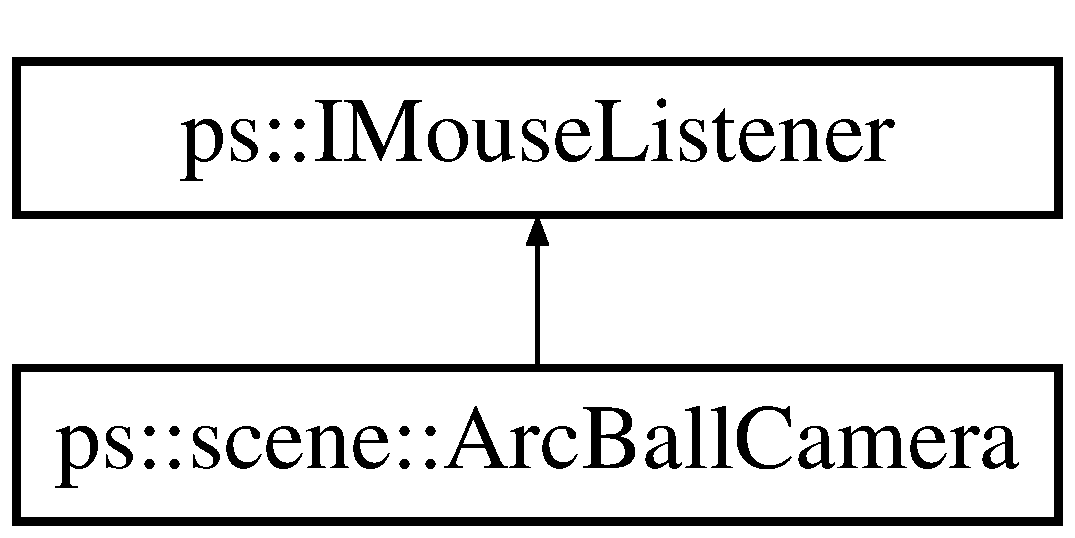
\includegraphics[height=2.000000cm]{classps_1_1scene_1_1ArcBallCamera}
\end{center}
\end{figure}
\subsection*{Public Member Functions}
\begin{DoxyCompactItemize}
\item 
\hypertarget{classps_1_1scene_1_1ArcBallCamera_a547389f27ab9e3995b953008b6306ac2}{}{\bfseries Arc\+Ball\+Camera} (float roll, float tilt, float zoom)\label{classps_1_1scene_1_1ArcBallCamera_a547389f27ab9e3995b953008b6306ac2}

\item 
\hypertarget{classps_1_1scene_1_1ArcBallCamera_a15aefd2b4d416b066959d8b46ad92b1c}{}void {\bfseries look} () const \label{classps_1_1scene_1_1ArcBallCamera_a15aefd2b4d416b066959d8b46ad92b1c}

\item 
\hypertarget{classps_1_1scene_1_1ArcBallCamera_ae70625ca7be7003f20afdc26ecc4dd06}{}float {\bfseries roll} () const \label{classps_1_1scene_1_1ArcBallCamera_ae70625ca7be7003f20afdc26ecc4dd06}

\item 
\hypertarget{classps_1_1scene_1_1ArcBallCamera_a30b95e4c33decfcf74d59b9c4d4858bf}{}void {\bfseries set\+Roll} (float roll\+H\+Deg)\label{classps_1_1scene_1_1ArcBallCamera_a30b95e4c33decfcf74d59b9c4d4858bf}

\item 
\hypertarget{classps_1_1scene_1_1ArcBallCamera_a78d152d433db1038295061c6248e2f0f}{}float {\bfseries tilt} () const \label{classps_1_1scene_1_1ArcBallCamera_a78d152d433db1038295061c6248e2f0f}

\item 
\hypertarget{classps_1_1scene_1_1ArcBallCamera_a9ec90b07a1b07be7280c7f3856130ccb}{}void {\bfseries set\+Tilt} (float tilt\+V\+Deg)\label{classps_1_1scene_1_1ArcBallCamera_a9ec90b07a1b07be7280c7f3856130ccb}

\item 
\hypertarget{classps_1_1scene_1_1ArcBallCamera_a144a4b47c76575b9577079fe7534c258}{}float {\bfseries zoomlevel} () const \label{classps_1_1scene_1_1ArcBallCamera_a144a4b47c76575b9577079fe7534c258}

\item 
\hypertarget{classps_1_1scene_1_1ArcBallCamera_a54d575e650e2a8bb35fa830409279852}{}void {\bfseries set\+Zoom\+Level} (float r)\label{classps_1_1scene_1_1ArcBallCamera_a54d575e650e2a8bb35fa830409279852}

\item 
\hypertarget{classps_1_1scene_1_1ArcBallCamera_ac1a5c192a1b489769aadf2a794dfa149}{}void {\bfseries incr\+Zoom\+Level} (float delta)\label{classps_1_1scene_1_1ArcBallCamera_ac1a5c192a1b489769aadf2a794dfa149}

\item 
\hypertarget{classps_1_1scene_1_1ArcBallCamera_a0b40beb8689d0db666b93746f3a473ab}{}\hyperlink{classps_1_1base_1_1Vec2}{vec2f} {\bfseries pan} () const \label{classps_1_1scene_1_1ArcBallCamera_a0b40beb8689d0db666b93746f3a473ab}

\item 
\hypertarget{classps_1_1scene_1_1ArcBallCamera_a7fcbb21e37c84b977f6d3b7d274d7d94}{}void {\bfseries set\+Pan} (const \hyperlink{classps_1_1base_1_1Vec2}{vec2f} \&pan)\label{classps_1_1scene_1_1ArcBallCamera_a7fcbb21e37c84b977f6d3b7d274d7d94}

\item 
\hypertarget{classps_1_1scene_1_1ArcBallCamera_a5ff35ac19e9a13be3b22508428369440}{}\hyperlink{classps_1_1base_1_1Vec3}{vec3f} {\bfseries origin} () const \label{classps_1_1scene_1_1ArcBallCamera_a5ff35ac19e9a13be3b22508428369440}

\item 
\hypertarget{classps_1_1scene_1_1ArcBallCamera_a1f71cb3e9521b2c3a5a0e57cfecd2420}{}void {\bfseries set\+Origin} (const \hyperlink{classps_1_1base_1_1Vec3}{vec3f} \&org)\label{classps_1_1scene_1_1ArcBallCamera_a1f71cb3e9521b2c3a5a0e57cfecd2420}

\item 
\hypertarget{classps_1_1scene_1_1ArcBallCamera_aae3bf9d81cc09964a94fcc2a385ad5cf}{}\hyperlink{classps_1_1base_1_1Vec3}{vec3f} {\bfseries center} () const \label{classps_1_1scene_1_1ArcBallCamera_aae3bf9d81cc09964a94fcc2a385ad5cf}

\item 
\hypertarget{classps_1_1scene_1_1ArcBallCamera_a3f76e247cc639117c8295579024ba173}{}void {\bfseries set\+Center} (const \hyperlink{classps_1_1base_1_1Vec3}{vec3f} \&c)\label{classps_1_1scene_1_1ArcBallCamera_a3f76e247cc639117c8295579024ba173}

\item 
\hypertarget{classps_1_1scene_1_1ArcBallCamera_a563746bfcff0743deda9be92a5017ec9}{}void {\bfseries mouse\+Press} (Mouse\+Button button, Mouse\+Button\+State state, int x, int y) override\label{classps_1_1scene_1_1ArcBallCamera_a563746bfcff0743deda9be92a5017ec9}

\item 
\hypertarget{classps_1_1scene_1_1ArcBallCamera_ad3337aef66263f061a69ec65a798515d}{}void {\bfseries mouse\+Move} (int x, int y) override\label{classps_1_1scene_1_1ArcBallCamera_ad3337aef66263f061a69ec65a798515d}

\item 
\hypertarget{classps_1_1scene_1_1ArcBallCamera_a925d91c15cdf870043f0e5ec53177ad9}{}void {\bfseries mouse\+Wheel} (Mouse\+Wheel\+Dir dir) override\label{classps_1_1scene_1_1ArcBallCamera_a925d91c15cdf870043f0e5ec53177ad9}

\item 
\hypertarget{classps_1_1scene_1_1ArcBallCamera_a5a5923f24d2bd9ed9574464d6df2b919}{}\hyperlink{classps_1_1base_1_1Vec3}{vec3f} {\bfseries pos} () const \label{classps_1_1scene_1_1ArcBallCamera_a5a5923f24d2bd9ed9574464d6df2b919}

\item 
\hypertarget{classps_1_1scene_1_1ArcBallCamera_a18e81e3f76219a1b551cac30d4bf5f0a}{}\hyperlink{classps_1_1base_1_1Vec3}{vec3f} {\bfseries direction} () const \label{classps_1_1scene_1_1ArcBallCamera_a18e81e3f76219a1b551cac30d4bf5f0a}

\item 
\hypertarget{classps_1_1scene_1_1ArcBallCamera_a770aec80b0ca6f7d2c7596d260f91d73}{}\hyperlink{classps_1_1base_1_1Vec3}{vec3f} {\bfseries up\+Vector} () const \label{classps_1_1scene_1_1ArcBallCamera_a770aec80b0ca6f7d2c7596d260f91d73}

\item 
\hypertarget{classps_1_1scene_1_1ArcBallCamera_a88ca6503a727f01ea624c99c56908775}{}\hyperlink{classps_1_1base_1_1Vec3}{vec3f} {\bfseries strafe} () const \label{classps_1_1scene_1_1ArcBallCamera_a88ca6503a727f01ea624c99c56908775}

\item 
\hypertarget{classps_1_1scene_1_1ArcBallCamera_a83dfa569db495758c6335dbb4fa7b904}{}\hyperlink{classps_1_1base_1_1Vec2}{vec2i} {\bfseries last\+Pos} () const \label{classps_1_1scene_1_1ArcBallCamera_a83dfa569db495758c6335dbb4fa7b904}

\item 
\hypertarget{classps_1_1scene_1_1ArcBallCamera_a4b136f05455f657f65dd51fc7f9e34a0}{}void {\bfseries set\+Last\+Pos} (const \hyperlink{classps_1_1base_1_1Vec2}{vec2i} \&last\+Pos)\label{classps_1_1scene_1_1ArcBallCamera_a4b136f05455f657f65dd51fc7f9e34a0}

\item 
\hypertarget{classps_1_1scene_1_1ArcBallCamera_a9b816ded6e436b8842fc9e94be354a7a}{}void {\bfseries compute\+Local\+Coordinate\+System} ()\label{classps_1_1scene_1_1ArcBallCamera_a9b816ded6e436b8842fc9e94be354a7a}

\item 
\hypertarget{classps_1_1scene_1_1ArcBallCamera_a2db509532bb2c8274ae099644e76a45a}{}void {\bfseries screen\+To\+World\+\_\+\+Orientation\+Only3\+D} (const \hyperlink{classps_1_1base_1_1Vec3}{vec3f} \&pt\+Screen, \hyperlink{classps_1_1base_1_1Vec3}{vec3f} \&pt\+World)\label{classps_1_1scene_1_1ArcBallCamera_a2db509532bb2c8274ae099644e76a45a}

\item 
\hypertarget{classps_1_1scene_1_1ArcBallCamera_aa519f086c713c26d53d98b331dc4f85f}{}void {\bfseries go\+Home} ()\label{classps_1_1scene_1_1ArcBallCamera_aa519f086c713c26d53d98b331dc4f85f}

\end{DoxyCompactItemize}
\subsection*{Additional Inherited Members}


The documentation for this class was generated from the following files\+:\begin{DoxyCompactItemize}
\item 
/\+Users/pourya/\+Desktop/platform/repos/tetcutter/src/scene/arcballcamera.\+h\item 
/\+Users/pourya/\+Desktop/platform/repos/tetcutter/src/scene/arcballcamera.\+cpp\end{DoxyCompactItemize}

\hypertarget{classps_1_1scene_1_1Asset}{}\section{ps\+:\+:scene\+:\+:Asset Class Reference}
\label{classps_1_1scene_1_1Asset}\index{ps\+::scene\+::\+Asset@{ps\+::scene\+::\+Asset}}
Inheritance diagram for ps\+:\+:scene\+:\+:Asset\+:\begin{figure}[H]
\begin{center}
\leavevmode
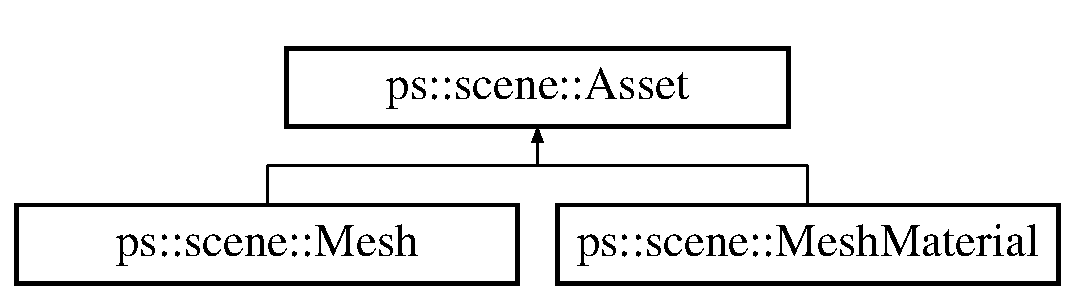
\includegraphics[height=2.000000cm]{classps_1_1scene_1_1Asset}
\end{center}
\end{figure}
\subsection*{Public Member Functions}
\begin{DoxyCompactItemize}
\item 
\hypertarget{classps_1_1scene_1_1Asset_a3cefe1397cff706fdd7f9f4a44974188}{}string {\bfseries name} () const \label{classps_1_1scene_1_1Asset_a3cefe1397cff706fdd7f9f4a44974188}

\item 
\hypertarget{classps_1_1scene_1_1Asset_ad7a73f290bbe2d6fd56e47470903b081}{}void {\bfseries set\+Name} (const string \&name)\label{classps_1_1scene_1_1Asset_ad7a73f290bbe2d6fd56e47470903b081}

\item 
\hypertarget{classps_1_1scene_1_1Asset_a2f61daf9e9cc7d04b949e94e4e9c1a8f}{}U64 {\bfseries last\+Accessed\+Time\+Stamp} ()\label{classps_1_1scene_1_1Asset_a2f61daf9e9cc7d04b949e94e4e9c1a8f}

\item 
\hypertarget{classps_1_1scene_1_1Asset_a348f6ba9e92844dc8abb43ac39069159}{}bool {\bfseries is\+Serializeable} () const \label{classps_1_1scene_1_1Asset_a348f6ba9e92844dc8abb43ac39069159}

\item 
\hypertarget{classps_1_1scene_1_1Asset_a3b2277636f3e92fcedad131ba0949f7d}{}virtual bool {\bfseries load} (const char $\ast$chr\+File\+Path)\label{classps_1_1scene_1_1Asset_a3b2277636f3e92fcedad131ba0949f7d}

\item 
\hypertarget{classps_1_1scene_1_1Asset_a64b74f1fc93c9c62ee0fc4e3060c5953}{}virtual bool {\bfseries store} (const char $\ast$chr\+File\+Path)\label{classps_1_1scene_1_1Asset_a64b74f1fc93c9c62ee0fc4e3060c5953}

\end{DoxyCompactItemize}
\subsection*{Protected Attributes}
\begin{DoxyCompactItemize}
\item 
\hypertarget{classps_1_1scene_1_1Asset_a6297f3ca1e396c083a610f1067bdce9a}{}bool {\bfseries m\+\_\+is\+Serializeable}\label{classps_1_1scene_1_1Asset_a6297f3ca1e396c083a610f1067bdce9a}

\item 
\hypertarget{classps_1_1scene_1_1Asset_a5575521b33ef60c798acb2d2fa95c532}{}U64 {\bfseries m\+\_\+ts\+Accessed}\label{classps_1_1scene_1_1Asset_a5575521b33ef60c798acb2d2fa95c532}

\item 
\hypertarget{classps_1_1scene_1_1Asset_a6f18386d1a1fd1f0cab5032ffd065d69}{}string {\bfseries m\+\_\+name}\label{classps_1_1scene_1_1Asset_a6f18386d1a1fd1f0cab5032ffd065d69}

\end{DoxyCompactItemize}


The documentation for this class was generated from the following files\+:\begin{DoxyCompactItemize}
\item 
/\+Users/pourya/\+Desktop/platform/repos/tetcutter/src/scene/sgassetmanager.\+h\item 
/\+Users/pourya/\+Desktop/platform/repos/tetcutter/src/scene/sgassetmanager.\+cpp\end{DoxyCompactItemize}

\hypertarget{classps_1_1scene_1_1AssetManager}{}\section{ps\+:\+:scene\+:\+:Asset\+Manager Class Reference}
\label{classps_1_1scene_1_1AssetManager}\index{ps\+::scene\+::\+Asset\+Manager@{ps\+::scene\+::\+Asset\+Manager}}


{\ttfamily \#include $<$sgassetmanager.\+h$>$}

Inheritance diagram for ps\+:\+:scene\+:\+:Asset\+Manager\+:\begin{figure}[H]
\begin{center}
\leavevmode
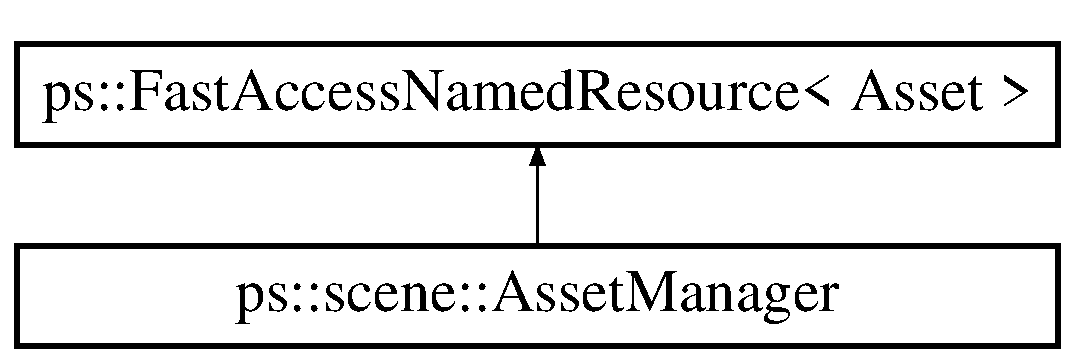
\includegraphics[height=2.000000cm]{classps_1_1scene_1_1AssetManager}
\end{center}
\end{figure}
\subsection*{Additional Inherited Members}


\subsection{Detailed Description}
\hyperlink{classps_1_1scene_1_1AssetManager}{Asset\+Manager} is a repository for all application assets which may include\+: 1.\+Textures 2.\+Meshes 3.\+Materials 4.\+Config files \hyperlink{classps_1_1scene_1_1Asset}{Asset} manager provides named access to the assets and an intelligent mechanism for releasing unused assets and accessing used ones. It can also log asset access information into an sqlite database with timing and detailed info. It can be further extended to be controlled by a network server of assets and requests to be fullfilled from those servers. 

The documentation for this class was generated from the following files\+:\begin{DoxyCompactItemize}
\item 
/\+Users/pourya/\+Desktop/platform/repos/tetcutter/src/scene/sgassetmanager.\+h\item 
/\+Users/pourya/\+Desktop/platform/repos/tetcutter/src/scene/sgassetmanager.\+cpp\end{DoxyCompactItemize}

\hypertarget{classps_1_1elastic_1_1AvatarRing}{}\section{ps\+:\+:elastic\+:\+:Avatar\+Ring Class Reference}
\label{classps_1_1elastic_1_1AvatarRing}\index{ps\+::elastic\+::\+Avatar\+Ring@{ps\+::elastic\+::\+Avatar\+Ring}}
Inheritance diagram for ps\+:\+:elastic\+:\+:Avatar\+Ring\+:\begin{figure}[H]
\begin{center}
\leavevmode
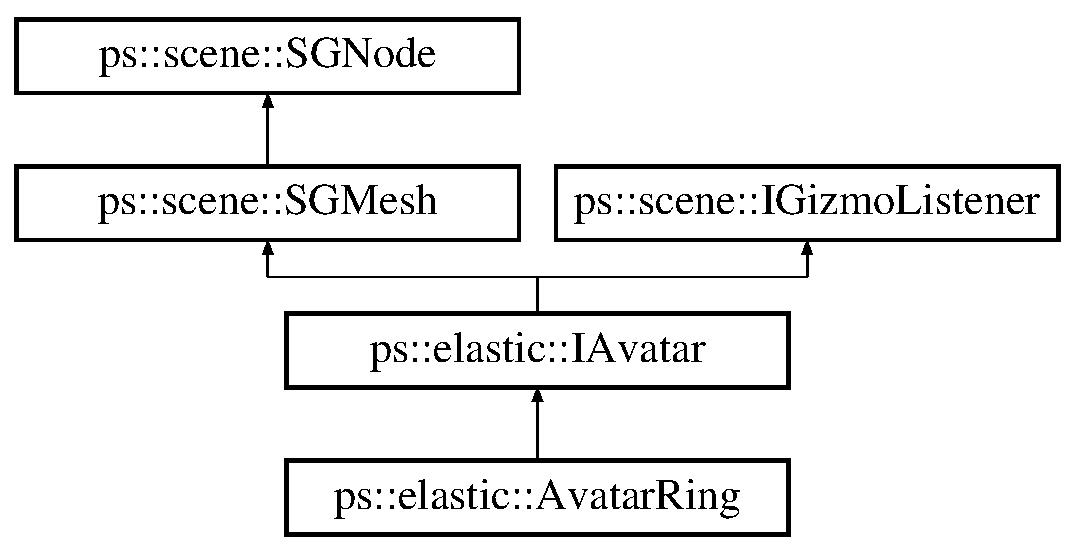
\includegraphics[height=4.000000cm]{classps_1_1elastic_1_1AvatarRing}
\end{center}
\end{figure}
\subsection*{Public Member Functions}
\begin{DoxyCompactItemize}
\item 
\hypertarget{classps_1_1elastic_1_1AvatarRing_ae7df8a8e69f621bab70d99aaa8c91403}{}{\bfseries Avatar\+Ring} (\hyperlink{classps_1_1opengl_1_1GLTexture}{G\+L\+Texture} $\ast$a\+Tex=N\+U\+L\+L)\label{classps_1_1elastic_1_1AvatarRing_ae7df8a8e69f621bab70d99aaa8c91403}

\item 
\hypertarget{classps_1_1elastic_1_1AvatarRing_a440d1593d71051c714e7c1ec63083027}{}void {\bfseries init} ()\label{classps_1_1elastic_1_1AvatarRing_a440d1593d71051c714e7c1ec63083027}

\item 
\hypertarget{classps_1_1elastic_1_1AvatarRing_a4cf7d4c4d18534929b9de180eae4ed1c}{}void {\bfseries draw} ()\label{classps_1_1elastic_1_1AvatarRing_a4cf7d4c4d18534929b9de180eae4ed1c}

\item 
\hypertarget{classps_1_1elastic_1_1AvatarRing_aa0e630ffc0c4b2c9b3195700953df4cf}{}void {\bfseries on\+Translate} (const \hyperlink{classps_1_1base_1_1Vec3}{vec3f} \&delta, const \hyperlink{classps_1_1base_1_1Vec3}{vec3f} \&pos) override\label{classps_1_1elastic_1_1AvatarRing_aa0e630ffc0c4b2c9b3195700953df4cf}

\item 
\hypertarget{classps_1_1elastic_1_1AvatarRing_a92f03a4a1acc9adbb062567d7c9fc285}{}void {\bfseries clear\+Cut\+Context} ()\label{classps_1_1elastic_1_1AvatarRing_a92f03a4a1acc9adbb062567d7c9fc285}

\end{DoxyCompactItemize}
\subsection*{Protected Attributes}
\begin{DoxyCompactItemize}
\item 
\hypertarget{classps_1_1elastic_1_1AvatarRing_a46a04664d4db6971e1cd1e42ac60245f}{}\hyperlink{classps_1_1opengl_1_1GLTexture}{G\+L\+Texture} $\ast$ {\bfseries m\+\_\+lp\+Tex}\label{classps_1_1elastic_1_1AvatarRing_a46a04664d4db6971e1cd1e42ac60245f}

\item 
\hypertarget{classps_1_1elastic_1_1AvatarRing_abcbabd52877cb7afaaf4d416e269f350}{}bool {\bfseries m\+\_\+is\+Swept\+Quad\+Valid}\label{classps_1_1elastic_1_1AvatarRing_abcbabd52877cb7afaaf4d416e269f350}

\item 
\hypertarget{classps_1_1elastic_1_1AvatarRing_a116e98b8de4979ff971fb4e53183e59d}{}\hyperlink{classps_1_1base_1_1AABB}{A\+A\+B\+B} {\bfseries m\+\_\+aabb\+Current}\label{classps_1_1elastic_1_1AvatarRing_a116e98b8de4979ff971fb4e53183e59d}

\item 
\hypertarget{classps_1_1elastic_1_1AvatarRing_ab5dc27bad648a315b9b27f1e14fa3997}{}\hyperlink{classps_1_1scene_1_1SGMesh}{S\+G\+Mesh} {\bfseries m\+\_\+outline}\label{classps_1_1elastic_1_1AvatarRing_ab5dc27bad648a315b9b27f1e14fa3997}

\item 
\hypertarget{classps_1_1elastic_1_1AvatarRing_a9888ec2e2739172429c1702f7eb43064}{}vector$<$ \hyperlink{classps_1_1base_1_1Vec3}{vec3d} $>$ {\bfseries m\+\_\+v\+Cutting\+Path}\label{classps_1_1elastic_1_1AvatarRing_a9888ec2e2739172429c1702f7eb43064}

\item 
\hypertarget{classps_1_1elastic_1_1AvatarRing_a9c07a64af879c499496ca96329dccc60}{}vector$<$ \hyperlink{classps_1_1base_1_1Vec3}{vec3d} $>$ {\bfseries m\+\_\+v\+Swept\+Quads}\label{classps_1_1elastic_1_1AvatarRing_a9c07a64af879c499496ca96329dccc60}

\item 
\hypertarget{classps_1_1elastic_1_1AvatarRing_ab70049777e6fa0219fc01134c69201a6}{}vector$<$ \hyperlink{classps_1_1base_1_1Vec3}{vec3d} $>$ {\bfseries m\+\_\+v\+Segments\+Ref}\label{classps_1_1elastic_1_1AvatarRing_ab70049777e6fa0219fc01134c69201a6}

\item 
\hypertarget{classps_1_1elastic_1_1AvatarRing_ab57af0fbd60248fea589c259df576643}{}vector$<$ \hyperlink{classps_1_1base_1_1Vec3}{vec3d} $>$ {\bfseries m\+\_\+v\+Segments\+Cur}\label{classps_1_1elastic_1_1AvatarRing_ab57af0fbd60248fea589c259df576643}

\end{DoxyCompactItemize}
\subsection*{Additional Inherited Members}


The documentation for this class was generated from the following files\+:\begin{DoxyCompactItemize}
\item 
/\+Users/pourya/\+Desktop/platform/repos/tetcutter/src/elastic/avatarring.\+h\item 
/\+Users/pourya/\+Desktop/platform/repos/tetcutter/src/elastic/avatarring.\+cpp\end{DoxyCompactItemize}

\hypertarget{classps_1_1elastic_1_1AvatarScalpel}{}\section{ps\+:\+:elastic\+:\+:Avatar\+Scalpel Class Reference}
\label{classps_1_1elastic_1_1AvatarScalpel}\index{ps\+::elastic\+::\+Avatar\+Scalpel@{ps\+::elastic\+::\+Avatar\+Scalpel}}


{\ttfamily \#include $<$avatarscalpel.\+h$>$}

Inheritance diagram for ps\+:\+:elastic\+:\+:Avatar\+Scalpel\+:\begin{figure}[H]
\begin{center}
\leavevmode
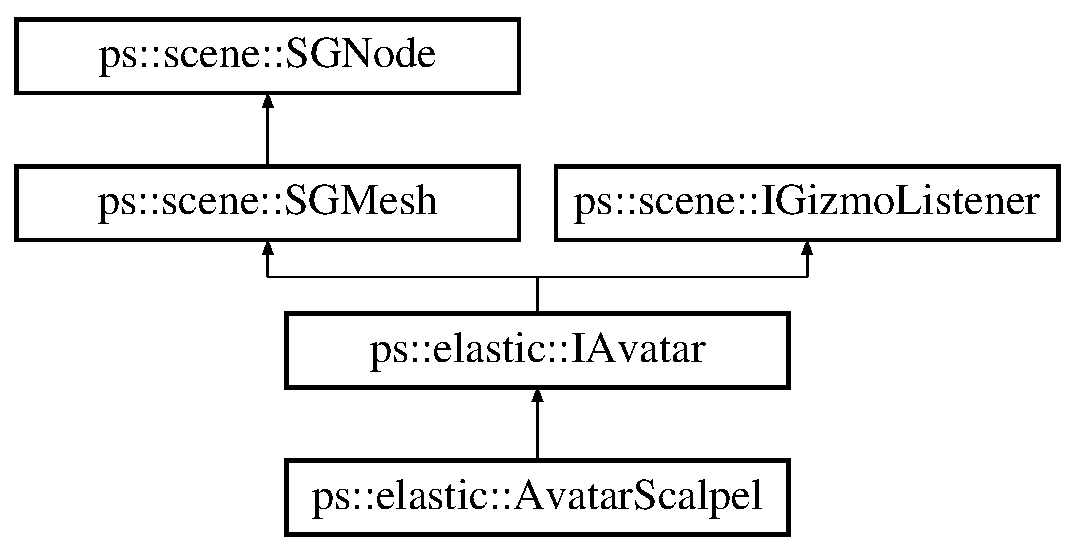
\includegraphics[height=4.000000cm]{classps_1_1elastic_1_1AvatarScalpel}
\end{center}
\end{figure}
\subsection*{Public Member Functions}
\begin{DoxyCompactItemize}
\item 
\hypertarget{classps_1_1elastic_1_1AvatarScalpel_a2e65c2453c121bec800f2b11acb60d7b}{}{\bfseries Avatar\+Scalpel} (\hyperlink{classps_1_1elastic_1_1CuttableMesh}{Cuttable\+Mesh} $\ast$tissue)\label{classps_1_1elastic_1_1AvatarScalpel_a2e65c2453c121bec800f2b11acb60d7b}

\item 
\hypertarget{classps_1_1elastic_1_1AvatarScalpel_a76a06347e93bc6a7b3468ae6f9212db1}{}void {\bfseries init} ()\label{classps_1_1elastic_1_1AvatarScalpel_a76a06347e93bc6a7b3468ae6f9212db1}

\item 
\hypertarget{classps_1_1elastic_1_1AvatarScalpel_aecf0e668fb5301ee45c169fd9aaed8e9}{}void {\bfseries draw} ()\label{classps_1_1elastic_1_1AvatarScalpel_aecf0e668fb5301ee45c169fd9aaed8e9}

\item 
\hypertarget{classps_1_1elastic_1_1AvatarScalpel_a9e40e85b2cdbaceb1cfc1ed6436240ff}{}void {\bfseries on\+Translate} (const \hyperlink{classps_1_1base_1_1Vec3}{vec3f} \&delta, const \hyperlink{classps_1_1base_1_1Vec3}{vec3f} \&pos) override\label{classps_1_1elastic_1_1AvatarScalpel_a9e40e85b2cdbaceb1cfc1ed6436240ff}

\item 
\hypertarget{classps_1_1elastic_1_1AvatarScalpel_a65f829ad9e630c99cb6370698782fb0c}{}void {\bfseries clear\+Cut\+Context} ()\label{classps_1_1elastic_1_1AvatarScalpel_a65f829ad9e630c99cb6370698782fb0c}

\end{DoxyCompactItemize}
\subsection*{Protected Attributes}
\begin{DoxyCompactItemize}
\item 
\hypertarget{classps_1_1elastic_1_1AvatarScalpel_ab2e43d4a992f701379724ff7dffbde35}{}bool {\bfseries m\+\_\+is\+Swept\+Quad\+Valid}\label{classps_1_1elastic_1_1AvatarScalpel_ab2e43d4a992f701379724ff7dffbde35}

\item 
\hypertarget{classps_1_1elastic_1_1AvatarScalpel_af2654d1671a3769317072a86e2a4152e}{}\hyperlink{classps_1_1base_1_1AABB}{A\+A\+B\+B} {\bfseries m\+\_\+aabb\+Current}\label{classps_1_1elastic_1_1AvatarScalpel_af2654d1671a3769317072a86e2a4152e}

\item 
\hypertarget{classps_1_1elastic_1_1AvatarScalpel_abba156dd6af6695d827ae042d5b33466}{}\hyperlink{classps_1_1scene_1_1SGMesh}{S\+G\+Mesh} {\bfseries m\+\_\+outline}\label{classps_1_1elastic_1_1AvatarScalpel_abba156dd6af6695d827ae042d5b33466}

\item 
\hypertarget{classps_1_1elastic_1_1AvatarScalpel_a6b9e38d2000f71dc20d42c71bd34bd35}{}\hyperlink{classps_1_1base_1_1Vec3}{vec3f} {\bfseries m\+\_\+edgeref0}\label{classps_1_1elastic_1_1AvatarScalpel_a6b9e38d2000f71dc20d42c71bd34bd35}

\item 
\hypertarget{classps_1_1elastic_1_1AvatarScalpel_ae09c71b1a8eb1bca9acbfad133be224a}{}\hyperlink{classps_1_1base_1_1Vec3}{vec3f} {\bfseries m\+\_\+edgeref1}\label{classps_1_1elastic_1_1AvatarScalpel_ae09c71b1a8eb1bca9acbfad133be224a}

\item 
\hypertarget{classps_1_1elastic_1_1AvatarScalpel_a4f965eda4cc93346365879c5a724535e}{}vector$<$ \hyperlink{classps_1_1base_1_1Vec3}{vec3d} $>$ {\bfseries m\+\_\+v\+Cutting\+Path\+Edge0}\label{classps_1_1elastic_1_1AvatarScalpel_a4f965eda4cc93346365879c5a724535e}

\item 
\hypertarget{classps_1_1elastic_1_1AvatarScalpel_a6978076ffd3b8008ef85f3f626d1dda9}{}vector$<$ \hyperlink{classps_1_1base_1_1Vec3}{vec3d} $>$ {\bfseries m\+\_\+v\+Cutting\+Path\+Edge1}\label{classps_1_1elastic_1_1AvatarScalpel_a6978076ffd3b8008ef85f3f626d1dda9}

\item 
\hypertarget{classps_1_1elastic_1_1AvatarScalpel_a13ba4c4f954ab892a9a6ae9a09b45227}{}vector$<$ \hyperlink{classps_1_1base_1_1Vec3}{vec3d} $>$ {\bfseries m\+\_\+v\+Swept\+Quad}\label{classps_1_1elastic_1_1AvatarScalpel_a13ba4c4f954ab892a9a6ae9a09b45227}

\item 
\hypertarget{classps_1_1elastic_1_1AvatarScalpel_a54525ce26101d8faf1af48e0335bedee}{}vector$<$ \hyperlink{classps_1_1base_1_1Vec3}{vec3d} $>$ {\bfseries m\+\_\+v\+Blade\+Segments}\label{classps_1_1elastic_1_1AvatarScalpel_a54525ce26101d8faf1af48e0335bedee}

\end{DoxyCompactItemize}
\subsection*{Additional Inherited Members}


\subsection{Detailed Description}
Synopsis\+: Haptics Avatar guide 

The documentation for this class was generated from the following files\+:\begin{DoxyCompactItemize}
\item 
/\+Users/pourya/\+Desktop/platform/repos/tetcutter/src/elastic/avatarscalpel.\+h\item 
/\+Users/pourya/\+Desktop/platform/repos/tetcutter/src/elastic/avatarscalpel.\+cpp\end{DoxyCompactItemize}

\hypertarget{classps_1_1elastic_1_1BaseLink}{}\section{ps\+:\+:elastic\+:\+:Base\+Link Class Reference}
\label{classps_1_1elastic_1_1BaseLink}\index{ps\+::elastic\+::\+Base\+Link@{ps\+::elastic\+::\+Base\+Link}}
Inheritance diagram for ps\+:\+:elastic\+:\+:Base\+Link\+:\begin{figure}[H]
\begin{center}
\leavevmode
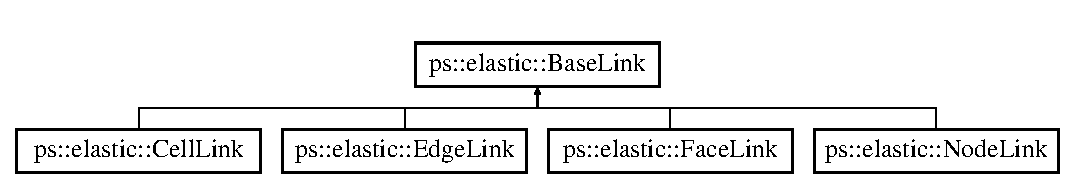
\includegraphics[height=2.000000cm]{classps_1_1elastic_1_1BaseLink}
\end{center}
\end{figure}
\subsection*{Public Member Functions}
\begin{DoxyCompactItemize}
\item 
\hypertarget{classps_1_1elastic_1_1BaseLink_a9782115132aa0cf585e19f2e1a8080e3}{}{\bfseries Base\+Link} (U32 idx)\label{classps_1_1elastic_1_1BaseLink_a9782115132aa0cf585e19f2e1a8080e3}

\item 
\hypertarget{classps_1_1elastic_1_1BaseLink_a12272e68539d931afe76837154ec4667}{}{\bfseries Base\+Link} (const \hyperlink{classps_1_1elastic_1_1BaseLink}{Base\+Link} \&other)\label{classps_1_1elastic_1_1BaseLink_a12272e68539d931afe76837154ec4667}

\item 
\hypertarget{classps_1_1elastic_1_1BaseLink_a351c1661413c026fe0abf7af3e704ee1}{}bool {\bfseries is\+Valid} () const \label{classps_1_1elastic_1_1BaseLink_a351c1661413c026fe0abf7af3e704ee1}

\item 
\hypertarget{classps_1_1elastic_1_1BaseLink_ac6e2d8c5c54501ad8dcce9fe750d8e9b}{}\hyperlink{classps_1_1elastic_1_1BaseLink}{Base\+Link} \& {\bfseries operator=} (const \hyperlink{classps_1_1elastic_1_1BaseLink}{Base\+Link} \&other)\label{classps_1_1elastic_1_1BaseLink_ac6e2d8c5c54501ad8dcce9fe750d8e9b}

\item 
\hypertarget{classps_1_1elastic_1_1BaseLink_a5c4260217360ce8b4f213863ddecfc8e}{}\hyperlink{classps_1_1elastic_1_1BaseLink}{Base\+Link} \& {\bfseries operator=} (U32 idx)\label{classps_1_1elastic_1_1BaseLink_a5c4260217360ce8b4f213863ddecfc8e}

\item 
\hypertarget{classps_1_1elastic_1_1BaseLink_abeac0c93efc1ef587441cb3eff0a494a}{}bool {\bfseries operator$<$} (const \hyperlink{classps_1_1elastic_1_1BaseLink}{Base\+Link} \&other) const \label{classps_1_1elastic_1_1BaseLink_abeac0c93efc1ef587441cb3eff0a494a}

\item 
\hypertarget{classps_1_1elastic_1_1BaseLink_a40f791d588097240cebb388bc47390e3}{}bool {\bfseries operator$>$} (const \hyperlink{classps_1_1elastic_1_1BaseLink}{Base\+Link} \&other) const \label{classps_1_1elastic_1_1BaseLink_a40f791d588097240cebb388bc47390e3}

\item 
\hypertarget{classps_1_1elastic_1_1BaseLink_a706acda6f6ac41ea842661ba3e69cf42}{}bool {\bfseries operator==} (const \hyperlink{classps_1_1elastic_1_1BaseLink}{Base\+Link} \&other) const \label{classps_1_1elastic_1_1BaseLink_a706acda6f6ac41ea842661ba3e69cf42}

\item 
\hypertarget{classps_1_1elastic_1_1BaseLink_acf6f28acf1d30ebd63948b1583d3323a}{}bool {\bfseries operator$<$} (U32 idx) const \label{classps_1_1elastic_1_1BaseLink_acf6f28acf1d30ebd63948b1583d3323a}

\item 
\hypertarget{classps_1_1elastic_1_1BaseLink_a0e023e71db4b8b7224b082cf2431692f}{}bool {\bfseries operator$>$} (U32 idx) const \label{classps_1_1elastic_1_1BaseLink_a0e023e71db4b8b7224b082cf2431692f}

\item 
\hypertarget{classps_1_1elastic_1_1BaseLink_a3787dd9498760d3eb872804990d11318}{}bool {\bfseries operator==} (U32 idx) const \label{classps_1_1elastic_1_1BaseLink_a3787dd9498760d3eb872804990d11318}

\item 
\hypertarget{classps_1_1elastic_1_1BaseLink_aca83fb5611e3a0ec6475761f60e6ff77}{}{\bfseries operator U32} () const \label{classps_1_1elastic_1_1BaseLink_aca83fb5611e3a0ec6475761f60e6ff77}

\end{DoxyCompactItemize}
\subsection*{Static Public Attributes}
\begin{DoxyCompactItemize}
\item 
\hypertarget{classps_1_1elastic_1_1BaseLink_a37307d433d8183e8448b6683c1abcf12}{}static const U32 {\bfseries I\+N\+V\+A\+L\+I\+D} = -\/1\label{classps_1_1elastic_1_1BaseLink_a37307d433d8183e8448b6683c1abcf12}

\end{DoxyCompactItemize}
\subsection*{Protected Attributes}
\begin{DoxyCompactItemize}
\item 
\hypertarget{classps_1_1elastic_1_1BaseLink_a78015f23c6888befc7d6779734b4cda4}{}U32 {\bfseries m\+\_\+idx}\label{classps_1_1elastic_1_1BaseLink_a78015f23c6888befc7d6779734b4cda4}

\end{DoxyCompactItemize}


The documentation for this class was generated from the following file\+:\begin{DoxyCompactItemize}
\item 
/\+Users/pourya/\+Desktop/platform/repos/tetcutter/src/elastic/volmeshentities.\+h\end{DoxyCompactItemize}

\hypertarget{classps_1_1base_1_1CAString}{}\section{ps\+:\+:base\+:\+:C\+A\+String Class Reference}
\label{classps_1_1base_1_1CAString}\index{ps\+::base\+::\+C\+A\+String@{ps\+::base\+::\+C\+A\+String}}
Inheritance diagram for ps\+:\+:base\+:\+:C\+A\+String\+:\begin{figure}[H]
\begin{center}
\leavevmode
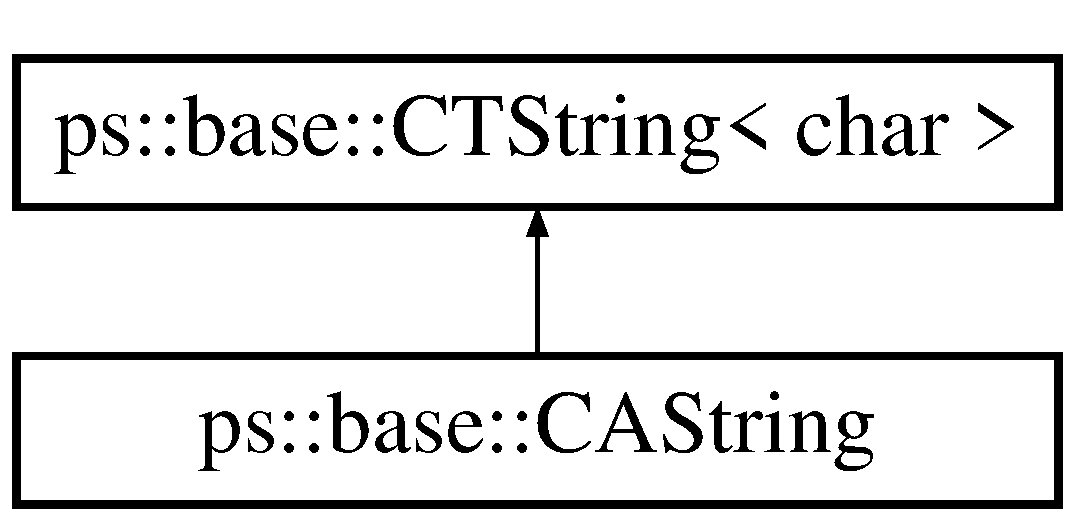
\includegraphics[height=2.000000cm]{classps_1_1base_1_1CAString}
\end{center}
\end{figure}
\subsection*{Public Types}
\begin{DoxyCompactItemize}
\item 
\hypertarget{classps_1_1base_1_1CAString_a73ee0ab6eb0d2990f70862a566ee9cca}{}typedef char {\bfseries U\+N\+I\+T}\label{classps_1_1base_1_1CAString_a73ee0ab6eb0d2990f70862a566ee9cca}

\end{DoxyCompactItemize}
\subsection*{Public Member Functions}
\begin{DoxyCompactItemize}
\item 
\hypertarget{classps_1_1base_1_1CAString_a0379a45cc9d7af8b05fcd0f89d919dfb}{}{\bfseries C\+A\+String} (const wchar\+\_\+t src\mbox{[}$\,$\mbox{]}, int src\+Size=0)\label{classps_1_1base_1_1CAString_a0379a45cc9d7af8b05fcd0f89d919dfb}

\item 
\hypertarget{classps_1_1base_1_1CAString_a86cd1efd75f0c634e0e770225b857651}{}{\bfseries C\+A\+String} (const char src\mbox{[}$\,$\mbox{]}, int src\+Size=0)\label{classps_1_1base_1_1CAString_a86cd1efd75f0c634e0e770225b857651}

\item 
\hypertarget{classps_1_1base_1_1CAString_af1140563e7daf47ebbb118b99395da1b}{}{\bfseries C\+A\+String} (const \hyperlink{classps_1_1base_1_1CAString}{C\+A\+String} \&src)\label{classps_1_1base_1_1CAString_af1140563e7daf47ebbb118b99395da1b}

\item 
\hypertarget{classps_1_1base_1_1CAString_ab74f898cdf853e08618d263284588137}{}int {\bfseries get\+Input\+Length} (const char src\mbox{[}$\,$\mbox{]}) const \label{classps_1_1base_1_1CAString_ab74f898cdf853e08618d263284588137}

\item 
\hypertarget{classps_1_1base_1_1CAString_a3a7b972ebcd1f5f94dd8a4c2703a5ebc}{}int {\bfseries get\+Input\+Length\+W} (const wchar\+\_\+t src\mbox{[}$\,$\mbox{]}) const \label{classps_1_1base_1_1CAString_a3a7b972ebcd1f5f94dd8a4c2703a5ebc}

\item 
\hypertarget{classps_1_1base_1_1CAString_acba7036f62ad1d3959930a67cee62a13}{}void {\bfseries copy\+From\+W} (const wchar\+\_\+t src\mbox{[}$\,$\mbox{]}, int src\+Size=0)\label{classps_1_1base_1_1CAString_acba7036f62ad1d3959930a67cee62a13}

\item 
\hypertarget{classps_1_1base_1_1CAString_ac258c7ac6666a65dceef6311f0e6a7aa}{}void {\bfseries append\+From\+W} (const wchar\+\_\+t src\mbox{[}$\,$\mbox{]}, int src\+Size=0)\label{classps_1_1base_1_1CAString_ac258c7ac6666a65dceef6311f0e6a7aa}

\item 
\hypertarget{classps_1_1base_1_1CAString_a7b42022933d843363fb56f4a57702dd0}{}void {\bfseries append\+From\+W} (const wchar\+\_\+t wch)\label{classps_1_1base_1_1CAString_a7b42022933d843363fb56f4a57702dd0}

\item 
\hypertarget{classps_1_1base_1_1CAString_a51f3ad8dad45d488d4d4c96133271571}{}int {\bfseries decompose} (const char delimiter, std\+::vector$<$ \hyperlink{classps_1_1base_1_1CAString}{C\+A\+String} $>$ \&lst\+Words) const \label{classps_1_1base_1_1CAString_a51f3ad8dad45d488d4d4c96133271571}

\item 
\hypertarget{classps_1_1base_1_1CAString_aeeb6fbc59f0567543b4c4dbd90be8a80}{}bool {\bfseries lcompare} (const char chr\+Buffer\mbox{[}$\,$\mbox{]}, int buf\+Size=0) const \label{classps_1_1base_1_1CAString_aeeb6fbc59f0567543b4c4dbd90be8a80}

\item 
\hypertarget{classps_1_1base_1_1CAString_a938de78124daf55637338f4fcddad31f}{}\hyperlink{classps_1_1base_1_1CAString}{C\+A\+String} {\bfseries substr} (int offset, int count=-\/1) const \label{classps_1_1base_1_1CAString_a938de78124daf55637338f4fcddad31f}

\item 
\hypertarget{classps_1_1base_1_1CAString_acfea142771eb720a0e2433d6e535c56c}{}\hyperlink{classps_1_1base_1_1CAString}{C\+A\+String} \& {\bfseries to\+Upper} ()\label{classps_1_1base_1_1CAString_acfea142771eb720a0e2433d6e535c56c}

\item 
\hypertarget{classps_1_1base_1_1CAString_a40a873d428d0fb836d50c6c4f07859c5}{}\hyperlink{classps_1_1base_1_1CAString}{C\+A\+String} \& {\bfseries to\+Lower} ()\label{classps_1_1base_1_1CAString_a40a873d428d0fb836d50c6c4f07859c5}

\item 
\hypertarget{classps_1_1base_1_1CAString_a9ce1f921f381bc9f3b2cae03d876465d}{}\hyperlink{classps_1_1base_1_1CAString}{C\+A\+String} \& {\bfseries trim} ()\label{classps_1_1base_1_1CAString_a9ce1f921f381bc9f3b2cae03d876465d}

\item 
\hypertarget{classps_1_1base_1_1CAString_aa0cea8163cd952290ee47c803ce2fb07}{}\hyperlink{classps_1_1base_1_1CAString}{C\+A\+String} \& {\bfseries remove\+Start\+End\+Spaces} ()\label{classps_1_1base_1_1CAString_aa0cea8163cd952290ee47c803ce2fb07}

\item 
\hypertarget{classps_1_1base_1_1CAString_a2f0ce5937bb70b929d08d0ad4bff545e}{}\hyperlink{classps_1_1base_1_1CAString}{C\+A\+String} {\bfseries operator+} (const \hyperlink{classps_1_1base_1_1CAString}{C\+A\+String} \&src) const \label{classps_1_1base_1_1CAString_a2f0ce5937bb70b929d08d0ad4bff545e}

\item 
\hypertarget{classps_1_1base_1_1CAString_a2940b9bfdba572a9ab7f394120d68f69}{}\hyperlink{classps_1_1base_1_1CAString}{C\+A\+String} {\bfseries operator+} (const wchar\+\_\+t src\mbox{[}$\,$\mbox{]}) const \label{classps_1_1base_1_1CAString_a2940b9bfdba572a9ab7f394120d68f69}

\item 
\hypertarget{classps_1_1base_1_1CAString_ab758cdba182bd41cb9abdf9390a49f12}{}\hyperlink{classps_1_1base_1_1CAString}{C\+A\+String} {\bfseries operator+} (wchar\+\_\+t src\mbox{[}$\,$\mbox{]}) const \label{classps_1_1base_1_1CAString_ab758cdba182bd41cb9abdf9390a49f12}

\item 
\hypertarget{classps_1_1base_1_1CAString_a1ceec721b97a70bbb142eb74bbf47854}{}\hyperlink{classps_1_1base_1_1CAString}{C\+A\+String} {\bfseries operator+} (const char src\mbox{[}$\,$\mbox{]}) const \label{classps_1_1base_1_1CAString_a1ceec721b97a70bbb142eb74bbf47854}

\item 
\hypertarget{classps_1_1base_1_1CAString_ad64dae60ed7af39ddac6ebad831db890}{}\hyperlink{classps_1_1base_1_1CAString}{C\+A\+String} {\bfseries operator+} (char src\mbox{[}$\,$\mbox{]}) const \label{classps_1_1base_1_1CAString_ad64dae60ed7af39ddac6ebad831db890}

\item 
\hypertarget{classps_1_1base_1_1CAString_a394216088a9e031b9f86c111873043e9}{}\hyperlink{classps_1_1base_1_1CAString}{C\+A\+String} {\bfseries operator+} (const char ch) const \label{classps_1_1base_1_1CAString_a394216088a9e031b9f86c111873043e9}

\item 
\hypertarget{classps_1_1base_1_1CAString_a8cf56b908ff64e1dd3e973a246d1bfe3}{}\hyperlink{classps_1_1base_1_1CAString}{C\+A\+String} {\bfseries operator+} (const wchar\+\_\+t ch) const \label{classps_1_1base_1_1CAString_a8cf56b908ff64e1dd3e973a246d1bfe3}

\item 
\hypertarget{classps_1_1base_1_1CAString_a5dbdb4bf8c0048edac587f7510f8d5ee}{}void {\bfseries operator+=} (const \hyperlink{classps_1_1base_1_1CAString}{C\+A\+String} \&src)\label{classps_1_1base_1_1CAString_a5dbdb4bf8c0048edac587f7510f8d5ee}

\item 
\hypertarget{classps_1_1base_1_1CAString_a79cfe4d43b9a81dbfded6117c460187f}{}void {\bfseries operator+=} (const wchar\+\_\+t src\mbox{[}$\,$\mbox{]})\label{classps_1_1base_1_1CAString_a79cfe4d43b9a81dbfded6117c460187f}

\item 
\hypertarget{classps_1_1base_1_1CAString_a849cbaa73841fa62de4689fb459bfe26}{}void {\bfseries operator+=} (wchar\+\_\+t src\mbox{[}$\,$\mbox{]})\label{classps_1_1base_1_1CAString_a849cbaa73841fa62de4689fb459bfe26}

\item 
\hypertarget{classps_1_1base_1_1CAString_a9db12d39b45cb7cb045c0b7ba5da7510}{}void {\bfseries operator+=} (const char src\mbox{[}$\,$\mbox{]})\label{classps_1_1base_1_1CAString_a9db12d39b45cb7cb045c0b7ba5da7510}

\item 
\hypertarget{classps_1_1base_1_1CAString_a113e46cba6460b898e4b05348b405cbf}{}void {\bfseries operator+=} (char src\mbox{[}$\,$\mbox{]})\label{classps_1_1base_1_1CAString_a113e46cba6460b898e4b05348b405cbf}

\item 
\hypertarget{classps_1_1base_1_1CAString_aa93e9a79c28e12343f7ed132a3c6298f}{}void {\bfseries operator+=} (const char ch)\label{classps_1_1base_1_1CAString_aa93e9a79c28e12343f7ed132a3c6298f}

\item 
\hypertarget{classps_1_1base_1_1CAString_a04d6fb5eeddbc1d7a79bfda05536af8b}{}void {\bfseries operator+=} (const wchar\+\_\+t ch)\label{classps_1_1base_1_1CAString_a04d6fb5eeddbc1d7a79bfda05536af8b}

\item 
\hypertarget{classps_1_1base_1_1CAString_ab2e5ea375e9400017ebaef067f631902}{}void {\bfseries operator=} (const char src\mbox{[}$\,$\mbox{]})\label{classps_1_1base_1_1CAString_ab2e5ea375e9400017ebaef067f631902}

\item 
\hypertarget{classps_1_1base_1_1CAString_a529d9e387c5d3923349f8889ec484301}{}void {\bfseries operator=} (const wchar\+\_\+t src\mbox{[}$\,$\mbox{]})\label{classps_1_1base_1_1CAString_a529d9e387c5d3923349f8889ec484301}

\end{DoxyCompactItemize}
\subsection*{Friends}
\begin{DoxyCompactItemize}
\item 
\hypertarget{classps_1_1base_1_1CAString_af08d599a65a50bd5131168bc28ae3d79}{}bool {\bfseries operator==} (const \hyperlink{classps_1_1base_1_1CAString}{C\+A\+String} \&a, const \hyperlink{classps_1_1base_1_1CAString}{C\+A\+String} \&b)\label{classps_1_1base_1_1CAString_af08d599a65a50bd5131168bc28ae3d79}

\item 
\hypertarget{classps_1_1base_1_1CAString_aecfb2f974e22bd9e714731540f485fb1}{}bool {\bfseries operator!=} (const \hyperlink{classps_1_1base_1_1CAString}{C\+A\+String} \&a, const \hyperlink{classps_1_1base_1_1CAString}{C\+A\+String} \&b)\label{classps_1_1base_1_1CAString_aecfb2f974e22bd9e714731540f485fb1}

\item 
\hypertarget{classps_1_1base_1_1CAString_a62956ad2e84aaeb16a98f858b0f47c04}{}std\+::ostream \& {\bfseries operator$<$$<$} (std\+::ostream \&outs, const \hyperlink{classps_1_1base_1_1CAString}{C\+A\+String} \&src)\label{classps_1_1base_1_1CAString_a62956ad2e84aaeb16a98f858b0f47c04}

\item 
\hypertarget{classps_1_1base_1_1CAString_ac6302a1ff70b302727ac650d67e53c96}{}std\+::istream \& {\bfseries operator$>$$>$} (std\+::istream \&ins, \hyperlink{classps_1_1base_1_1CAString}{C\+A\+String} \&src)\label{classps_1_1base_1_1CAString_ac6302a1ff70b302727ac650d67e53c96}

\end{DoxyCompactItemize}
\subsection*{Additional Inherited Members}


The documentation for this class was generated from the following files\+:\begin{DoxyCompactItemize}
\item 
/\+Users/pourya/\+Desktop/platform/repos/tetcutter/src/base/str.\+h\item 
/\+Users/pourya/\+Desktop/platform/repos/tetcutter/src/base/str.\+cpp\end{DoxyCompactItemize}

\hypertarget{classps_1_1elastic_1_1CELL}{}\section{ps\+:\+:elastic\+:\+:C\+E\+L\+L Class Reference}
\label{classps_1_1elastic_1_1CELL}\index{ps\+::elastic\+::\+C\+E\+L\+L@{ps\+::elastic\+::\+C\+E\+L\+L}}
\subsection*{Public Member Functions}
\begin{DoxyCompactItemize}
\item 
\hypertarget{classps_1_1elastic_1_1CELL_ad8c777847d313a337fae70d551eb6bcb}{}void {\bfseries init} ()\label{classps_1_1elastic_1_1CELL_ad8c777847d313a337fae70d551eb6bcb}

\item 
\hypertarget{classps_1_1elastic_1_1CELL_a368cfd1dbcb72240b61c62e0dba5e715}{}\hyperlink{classps_1_1elastic_1_1CELL}{C\+E\+L\+L} \& {\bfseries operator=} (const \hyperlink{classps_1_1elastic_1_1CELL}{C\+E\+L\+L} \&A)\label{classps_1_1elastic_1_1CELL_a368cfd1dbcb72240b61c62e0dba5e715}

\end{DoxyCompactItemize}
\subsection*{Public Attributes}
\begin{DoxyCompactItemize}
\item 
\hypertarget{classps_1_1elastic_1_1CELL_a895b4ba0a0eddba0b4dedfa5677047f3}{}U32 {\bfseries nodes} \mbox{[}C\+O\+U\+N\+T\+\_\+\+C\+E\+L\+L\+\_\+\+N\+O\+D\+E\+S\mbox{]}\label{classps_1_1elastic_1_1CELL_a895b4ba0a0eddba0b4dedfa5677047f3}

\item 
\hypertarget{classps_1_1elastic_1_1CELL_a367779edf9ba18a162ef9abf70980679}{}U32 {\bfseries faces} \mbox{[}C\+O\+U\+N\+T\+\_\+\+C\+E\+L\+L\+\_\+\+F\+A\+C\+E\+S\mbox{]}\label{classps_1_1elastic_1_1CELL_a367779edf9ba18a162ef9abf70980679}

\item 
\hypertarget{classps_1_1elastic_1_1CELL_a770b037d1e6fa4456bcded2cb40dd64c}{}U32 {\bfseries edges} \mbox{[}C\+O\+U\+N\+T\+\_\+\+C\+E\+L\+L\+\_\+\+E\+D\+G\+E\+S\mbox{]}\label{classps_1_1elastic_1_1CELL_a770b037d1e6fa4456bcded2cb40dd64c}

\end{DoxyCompactItemize}


The documentation for this class was generated from the following file\+:\begin{DoxyCompactItemize}
\item 
/\+Users/pourya/\+Desktop/platform/repos/tetcutter/src/elastic/volmeshentities.\+h\end{DoxyCompactItemize}

\hypertarget{classps_1_1elastic_1_1CellLink}{}\section{ps\+:\+:elastic\+:\+:Cell\+Link Class Reference}
\label{classps_1_1elastic_1_1CellLink}\index{ps\+::elastic\+::\+Cell\+Link@{ps\+::elastic\+::\+Cell\+Link}}
Inheritance diagram for ps\+:\+:elastic\+:\+:Cell\+Link\+:\begin{figure}[H]
\begin{center}
\leavevmode
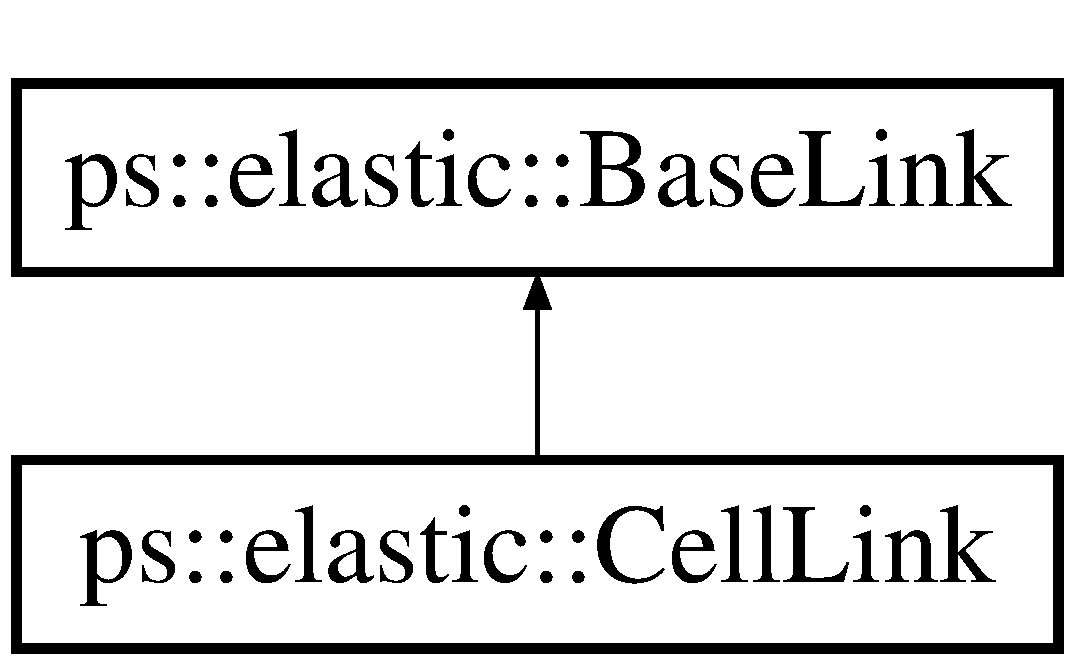
\includegraphics[height=2.000000cm]{classps_1_1elastic_1_1CellLink}
\end{center}
\end{figure}
\subsection*{Static Public Member Functions}
\begin{DoxyCompactItemize}
\item 
\hypertarget{classps_1_1elastic_1_1CellLink_a00f56f6c8708a51ad8d9588d7c6f2a7a}{}static \hyperlink{classps_1_1elastic_1_1CellLink}{Cell\+Link} {\bfseries create} (U32 idx)\label{classps_1_1elastic_1_1CellLink_a00f56f6c8708a51ad8d9588d7c6f2a7a}

\end{DoxyCompactItemize}
\subsection*{Additional Inherited Members}


The documentation for this class was generated from the following file\+:\begin{DoxyCompactItemize}
\item 
/\+Users/pourya/\+Desktop/platform/repos/tetcutter/src/elastic/volmeshentities.\+h\end{DoxyCompactItemize}

\hypertarget{classps_1_1utils_1_1CmdLineParser}{}\section{ps\+:\+:utils\+:\+:Cmd\+Line\+Parser Class Reference}
\label{classps_1_1utils_1_1CmdLineParser}\index{ps\+::utils\+::\+Cmd\+Line\+Parser@{ps\+::utils\+::\+Cmd\+Line\+Parser}}


{\ttfamily \#include $<$cmdlineparser.\+h$>$}

\subsection*{Classes}
\begin{DoxyCompactItemize}
\item 
class \hyperlink{classps_1_1utils_1_1CmdLineParser_1_1CmdSwitch}{Cmd\+Switch}
\end{DoxyCompactItemize}
\subsection*{Public Member Functions}
\begin{DoxyCompactItemize}
\item 
\hypertarget{classps_1_1utils_1_1CmdLineParser_a8167a43fc6b93e49aab170cc7189397d}{}bool {\bfseries add\+Switch} (const \hyperlink{classps_1_1utils_1_1CmdLineParser_1_1CmdSwitch}{Cmd\+Switch} \&s)\label{classps_1_1utils_1_1CmdLineParser_a8167a43fc6b93e49aab170cc7189397d}

\item 
\hypertarget{classps_1_1utils_1_1CmdLineParser_a97a17c25f257570a3d316cd5f5f48f01}{}bool {\bfseries add\+Switch} (const string \&name, const string \&shortcut, const string \&desc, const string \&default\+\_\+value=\char`\"{}\char`\"{}, bool istoggle=false)\label{classps_1_1utils_1_1CmdLineParser_a97a17c25f257570a3d316cd5f5f48f01}

\item 
bool \hyperlink{classps_1_1utils_1_1CmdLineParser_a20bf5b0d5bc797ccad37a08b7cca7a26}{set\+Default\+Key} (const char $\ast$key)
\item 
int \hyperlink{classps_1_1utils_1_1CmdLineParser_a3f665b3b1bde8f417809648d70390845}{parse} (int argc, char $\ast$argv\mbox{[}$\,$\mbox{]})
\item 
string \hyperlink{classps_1_1utils_1_1CmdLineParser_a5c39ac73b9ee3d312bef0f10db488cfb}{value} (const char $\ast$key)
\item 
\hypertarget{classps_1_1utils_1_1CmdLineParser_ae373b5a0d156b2a647c89fb98c68ed56}{}int {\bfseries value\+\_\+to\+\_\+int} (const char $\ast$key)\label{classps_1_1utils_1_1CmdLineParser_ae373b5a0d156b2a647c89fb98c68ed56}

\item 
\hypertarget{classps_1_1utils_1_1CmdLineParser_a925522c8f2711bf58dfca23125e37e9b}{}double {\bfseries value\+\_\+to\+\_\+double} (const char $\ast$key)\label{classps_1_1utils_1_1CmdLineParser_a925522c8f2711bf58dfca23125e37e9b}

\item 
bool \hyperlink{classps_1_1utils_1_1CmdLineParser_a4254b2a2312b6b6335cc8cb44dd185f1}{is\+Valid} (const char $\ast$key)
\item 
virtual void \hyperlink{classps_1_1utils_1_1CmdLineParser_a8619d5088b9532cc530198922f9bd253}{print\+Help} ()
\end{DoxyCompactItemize}
\subsection*{Protected Member Functions}
\begin{DoxyCompactItemize}
\item 
\hyperlink{classps_1_1utils_1_1CmdLineParser_1_1CmdSwitch}{Cmd\+Switch} $\ast$ \hyperlink{classps_1_1utils_1_1CmdLineParser_a2bd240e1eef347a201c955a50cc64dac}{get\+Cmd\+Switch} (const char $\ast$key)
\item 
\hypertarget{classps_1_1utils_1_1CmdLineParser_a6654e4f9d241476fe0ec62bd92ca71a8}{}bool {\bfseries token\+\_\+to\+\_\+fullkeyname} (const string \&token, string \&fullkey)\label{classps_1_1utils_1_1CmdLineParser_a6654e4f9d241476fe0ec62bd92ca71a8}

\end{DoxyCompactItemize}


\subsection{Detailed Description}
Synopsis\+: 1.\+Parses the command line passed in from the user and stores all enabled system options. 2.\+Prints help for the user if an option is not valid. 3.\+Stores options and provides a mechanism to read those options 

\subsection{Member Function Documentation}
\hypertarget{classps_1_1utils_1_1CmdLineParser_a2bd240e1eef347a201c955a50cc64dac}{}\index{ps\+::utils\+::\+Cmd\+Line\+Parser@{ps\+::utils\+::\+Cmd\+Line\+Parser}!get\+Cmd\+Switch@{get\+Cmd\+Switch}}
\index{get\+Cmd\+Switch@{get\+Cmd\+Switch}!ps\+::utils\+::\+Cmd\+Line\+Parser@{ps\+::utils\+::\+Cmd\+Line\+Parser}}
\subsubsection[{get\+Cmd\+Switch(const char $\ast$key)}]{\setlength{\rightskip}{0pt plus 5cm}{\bf Cmd\+Line\+Parser\+::\+Cmd\+Switch} $\ast$ ps\+::utils\+::\+Cmd\+Line\+Parser\+::get\+Cmd\+Switch (
\begin{DoxyParamCaption}
\item[{const char $\ast$}]{key}
\end{DoxyParamCaption}
)\hspace{0.3cm}{\ttfamily [protected]}}\label{classps_1_1utils_1_1CmdLineParser_a2bd240e1eef347a201c955a50cc64dac}
Retrieve command switch \hypertarget{classps_1_1utils_1_1CmdLineParser_a4254b2a2312b6b6335cc8cb44dd185f1}{}\index{ps\+::utils\+::\+Cmd\+Line\+Parser@{ps\+::utils\+::\+Cmd\+Line\+Parser}!is\+Valid@{is\+Valid}}
\index{is\+Valid@{is\+Valid}!ps\+::utils\+::\+Cmd\+Line\+Parser@{ps\+::utils\+::\+Cmd\+Line\+Parser}}
\subsubsection[{is\+Valid(const char $\ast$key)}]{\setlength{\rightskip}{0pt plus 5cm}bool ps\+::utils\+::\+Cmd\+Line\+Parser\+::is\+Valid (
\begin{DoxyParamCaption}
\item[{const char $\ast$}]{key}
\end{DoxyParamCaption}
)}\label{classps_1_1utils_1_1CmdLineParser_a4254b2a2312b6b6335cc8cb44dd185f1}
Returns true if a valid value is supplied by user \hypertarget{classps_1_1utils_1_1CmdLineParser_a3f665b3b1bde8f417809648d70390845}{}\index{ps\+::utils\+::\+Cmd\+Line\+Parser@{ps\+::utils\+::\+Cmd\+Line\+Parser}!parse@{parse}}
\index{parse@{parse}!ps\+::utils\+::\+Cmd\+Line\+Parser@{ps\+::utils\+::\+Cmd\+Line\+Parser}}
\subsubsection[{parse(int argc, char $\ast$argv[])}]{\setlength{\rightskip}{0pt plus 5cm}int ps\+::utils\+::\+Cmd\+Line\+Parser\+::parse (
\begin{DoxyParamCaption}
\item[{int}]{argc, }
\item[{char $\ast$}]{argv\mbox{[}$\,$\mbox{]}}
\end{DoxyParamCaption}
)}\label{classps_1_1utils_1_1CmdLineParser_a3f665b3b1bde8f417809648d70390845}
parse and store command line \hypertarget{classps_1_1utils_1_1CmdLineParser_a8619d5088b9532cc530198922f9bd253}{}\index{ps\+::utils\+::\+Cmd\+Line\+Parser@{ps\+::utils\+::\+Cmd\+Line\+Parser}!print\+Help@{print\+Help}}
\index{print\+Help@{print\+Help}!ps\+::utils\+::\+Cmd\+Line\+Parser@{ps\+::utils\+::\+Cmd\+Line\+Parser}}
\subsubsection[{print\+Help()}]{\setlength{\rightskip}{0pt plus 5cm}void ps\+::utils\+::\+Cmd\+Line\+Parser\+::print\+Help (
\begin{DoxyParamCaption}
{}
\end{DoxyParamCaption}
)\hspace{0.3cm}{\ttfamily [virtual]}}\label{classps_1_1utils_1_1CmdLineParser_a8619d5088b9532cc530198922f9bd253}
prints the help menu in case the options are not correct. \hypertarget{classps_1_1utils_1_1CmdLineParser_a20bf5b0d5bc797ccad37a08b7cca7a26}{}\index{ps\+::utils\+::\+Cmd\+Line\+Parser@{ps\+::utils\+::\+Cmd\+Line\+Parser}!set\+Default\+Key@{set\+Default\+Key}}
\index{set\+Default\+Key@{set\+Default\+Key}!ps\+::utils\+::\+Cmd\+Line\+Parser@{ps\+::utils\+::\+Cmd\+Line\+Parser}}
\subsubsection[{set\+Default\+Key(const char $\ast$key)}]{\setlength{\rightskip}{0pt plus 5cm}bool ps\+::utils\+::\+Cmd\+Line\+Parser\+::set\+Default\+Key (
\begin{DoxyParamCaption}
\item[{const char $\ast$}]{key}
\end{DoxyParamCaption}
)}\label{classps_1_1utils_1_1CmdLineParser_a20bf5b0d5bc797ccad37a08b7cca7a26}
sets default key to be able to read a 2 argumented call \hypertarget{classps_1_1utils_1_1CmdLineParser_a5c39ac73b9ee3d312bef0f10db488cfb}{}\index{ps\+::utils\+::\+Cmd\+Line\+Parser@{ps\+::utils\+::\+Cmd\+Line\+Parser}!value@{value}}
\index{value@{value}!ps\+::utils\+::\+Cmd\+Line\+Parser@{ps\+::utils\+::\+Cmd\+Line\+Parser}}
\subsubsection[{value(const char $\ast$key)}]{\setlength{\rightskip}{0pt plus 5cm}string ps\+::utils\+::\+Cmd\+Line\+Parser\+::value (
\begin{DoxyParamCaption}
\item[{const char $\ast$}]{key}
\end{DoxyParamCaption}
)}\label{classps_1_1utils_1_1CmdLineParser_a5c39ac73b9ee3d312bef0f10db488cfb}
retrieve value using a key 

The documentation for this class was generated from the following files\+:\begin{DoxyCompactItemize}
\item 
/\+Users/pourya/\+Desktop/platform/repos/tetcutter/src/base/cmdlineparser.\+h\item 
/\+Users/pourya/\+Desktop/platform/repos/tetcutter/src/base/cmdlineparser.\+cpp\end{DoxyCompactItemize}

\hypertarget{classps_1_1utils_1_1CmdLineParser_1_1CmdSwitch}{}\section{ps\+:\+:utils\+:\+:Cmd\+Line\+Parser\+:\+:Cmd\+Switch Class Reference}
\label{classps_1_1utils_1_1CmdLineParser_1_1CmdSwitch}\index{ps\+::utils\+::\+Cmd\+Line\+Parser\+::\+Cmd\+Switch@{ps\+::utils\+::\+Cmd\+Line\+Parser\+::\+Cmd\+Switch}}
\subsection*{Public Member Functions}
\begin{DoxyCompactItemize}
\item 
\hypertarget{classps_1_1utils_1_1CmdLineParser_1_1CmdSwitch_a801ddcda99803869be6f1f636cd65e98}{}{\bfseries Cmd\+Switch} (const \hyperlink{classps_1_1utils_1_1CmdLineParser_1_1CmdSwitch}{Cmd\+Switch} \&rhs)\label{classps_1_1utils_1_1CmdLineParser_1_1CmdSwitch_a801ddcda99803869be6f1f636cd65e98}

\item 
\hypertarget{classps_1_1utils_1_1CmdLineParser_1_1CmdSwitch_a727e5558f823d5abc7e8a89d383c2e3c}{}void {\bfseries copyfrom} (const \hyperlink{classps_1_1utils_1_1CmdLineParser_1_1CmdSwitch}{Cmd\+Switch} \&rhs)\label{classps_1_1utils_1_1CmdLineParser_1_1CmdSwitch_a727e5558f823d5abc7e8a89d383c2e3c}

\item 
\hypertarget{classps_1_1utils_1_1CmdLineParser_1_1CmdSwitch_a4c986bfc00ce55112cc702d18eb69cf3}{}\hyperlink{classps_1_1utils_1_1CmdLineParser_1_1CmdSwitch}{Cmd\+Switch} \& {\bfseries operator=} (const \hyperlink{classps_1_1utils_1_1CmdLineParser_1_1CmdSwitch}{Cmd\+Switch} \&rhs)\label{classps_1_1utils_1_1CmdLineParser_1_1CmdSwitch_a4c986bfc00ce55112cc702d18eb69cf3}

\end{DoxyCompactItemize}
\subsection*{Public Attributes}
\begin{DoxyCompactItemize}
\item 
\hypertarget{classps_1_1utils_1_1CmdLineParser_1_1CmdSwitch_a7699ec7daf9eacb532b8e8897c276ffc}{}string {\bfseries key}\label{classps_1_1utils_1_1CmdLineParser_1_1CmdSwitch_a7699ec7daf9eacb532b8e8897c276ffc}

\item 
\hypertarget{classps_1_1utils_1_1CmdLineParser_1_1CmdSwitch_ac97ba36cae224a21da7eed424439ad8a}{}string {\bfseries shortcut}\label{classps_1_1utils_1_1CmdLineParser_1_1CmdSwitch_ac97ba36cae224a21da7eed424439ad8a}

\item 
\hypertarget{classps_1_1utils_1_1CmdLineParser_1_1CmdSwitch_aab193ce5b2fa667c43b63ba47967430a}{}string {\bfseries default\+\_\+value}\label{classps_1_1utils_1_1CmdLineParser_1_1CmdSwitch_aab193ce5b2fa667c43b63ba47967430a}

\item 
\hypertarget{classps_1_1utils_1_1CmdLineParser_1_1CmdSwitch_a994fb96f31f902089e4995b3fcb30b67}{}string {\bfseries value}\label{classps_1_1utils_1_1CmdLineParser_1_1CmdSwitch_a994fb96f31f902089e4995b3fcb30b67}

\item 
\hypertarget{classps_1_1utils_1_1CmdLineParser_1_1CmdSwitch_a9be04c8c427e0f640a33795ded7986f2}{}string {\bfseries desc}\label{classps_1_1utils_1_1CmdLineParser_1_1CmdSwitch_a9be04c8c427e0f640a33795ded7986f2}

\item 
\hypertarget{classps_1_1utils_1_1CmdLineParser_1_1CmdSwitch_aae0efff071719d4eba1e3ef63b7d3063}{}bool {\bfseries istoggle}\label{classps_1_1utils_1_1CmdLineParser_1_1CmdSwitch_aae0efff071719d4eba1e3ef63b7d3063}

\item 
\hypertarget{classps_1_1utils_1_1CmdLineParser_1_1CmdSwitch_a01c1b146903579c92faff07d4624cdd1}{}bool {\bfseries isvalid}\label{classps_1_1utils_1_1CmdLineParser_1_1CmdSwitch_a01c1b146903579c92faff07d4624cdd1}

\end{DoxyCompactItemize}


The documentation for this class was generated from the following file\+:\begin{DoxyCompactItemize}
\item 
/\+Users/pourya/\+Desktop/platform/repos/tetcutter/src/base/cmdlineparser.\+h\end{DoxyCompactItemize}

\hypertarget{classps_1_1base_1_1Color}{}\section{ps\+:\+:base\+:\+:Color Class Reference}
\label{classps_1_1base_1_1Color}\index{ps\+::base\+::\+Color@{ps\+::base\+::\+Color}}
\subsection*{Public Member Functions}
\begin{DoxyCompactItemize}
\item 
\hypertarget{classps_1_1base_1_1Color_a0d181ae7453c014306dc421269d3d75f}{}{\bfseries Color} (U8 r, U8 g, U8 b, U8 a=255)\label{classps_1_1base_1_1Color_a0d181ae7453c014306dc421269d3d75f}

\item 
\hypertarget{classps_1_1base_1_1Color_aefa2f23b75ddd1f6e53873171730af52}{}{\bfseries Color} (const \hyperlink{classps_1_1base_1_1Vec4}{vec4u8} \&color)\label{classps_1_1base_1_1Color_aefa2f23b75ddd1f6e53873171730af52}

\item 
\hypertarget{classps_1_1base_1_1Color_a673509a46c18076d6052cc29d77f609b}{}{\bfseries Color} (const \hyperlink{classps_1_1base_1_1Vec4}{vec4f} \&color)\label{classps_1_1base_1_1Color_a673509a46c18076d6052cc29d77f609b}

\item 
\hypertarget{classps_1_1base_1_1Color_a352197899c03e28afb23355cb51add8a}{}{\bfseries Color} (const \hyperlink{classps_1_1base_1_1Color}{Color} \&other)\label{classps_1_1base_1_1Color_a352197899c03e28afb23355cb51add8a}

\item 
\hypertarget{classps_1_1base_1_1Color_ab2448085505743432ce86e7f38a425b3}{}void {\bfseries from\+R\+G\+B\+A} (const \hyperlink{classps_1_1base_1_1Vec4}{vec4u8} \&color)\label{classps_1_1base_1_1Color_ab2448085505743432ce86e7f38a425b3}

\item 
\hypertarget{classps_1_1base_1_1Color_a6b1e941f99dcafaf9c17e8c489fea035}{}void {\bfseries from\+R\+G\+B\+A} (U8 r, U8 g, U8 b, U8 a=255)\label{classps_1_1base_1_1Color_a6b1e941f99dcafaf9c17e8c489fea035}

\item 
\hypertarget{classps_1_1base_1_1Color_a5eb4aec1126afc0f2d30136b99eeb9f4}{}void {\bfseries from\+R\+G\+B\+A} (const \hyperlink{classps_1_1base_1_1Vec4}{vec4f} \&color)\label{classps_1_1base_1_1Color_a5eb4aec1126afc0f2d30136b99eeb9f4}

\item 
\hypertarget{classps_1_1base_1_1Color_a8e97d228ce88102b0111b65c3e3b784a}{}\hyperlink{classps_1_1base_1_1Vec4}{vec4f} {\bfseries to\+Vec4f} () const \label{classps_1_1base_1_1Color_a8e97d228ce88102b0111b65c3e3b784a}

\item 
\hypertarget{classps_1_1base_1_1Color_a342ea9135e1995ca8ac0f3c26942e3d5}{}\hyperlink{classps_1_1base_1_1Vec4}{vec4u8} {\bfseries to\+Vec4u8} () const \label{classps_1_1base_1_1Color_a342ea9135e1995ca8ac0f3c26942e3d5}

\item 
\hypertarget{classps_1_1base_1_1Color_afa699e0d1049f28c3ee29545c306b775}{}\hyperlink{classps_1_1base_1_1Color}{Color} \& {\bfseries operator=} (const \hyperlink{classps_1_1base_1_1Color}{Color} \&rhs)\label{classps_1_1base_1_1Color_afa699e0d1049f28c3ee29545c306b775}

\end{DoxyCompactItemize}
\subsection*{Static Public Member Functions}
\begin{DoxyCompactItemize}
\item 
\hypertarget{classps_1_1base_1_1Color_a287cd9aef06e5c646a26289fd5068618}{}static \hyperlink{classps_1_1base_1_1Color}{Color} {\bfseries red} ()\label{classps_1_1base_1_1Color_a287cd9aef06e5c646a26289fd5068618}

\item 
\hypertarget{classps_1_1base_1_1Color_ac63bc71202fa47a3e89ee134d59a57a4}{}static \hyperlink{classps_1_1base_1_1Color}{Color} {\bfseries green} ()\label{classps_1_1base_1_1Color_ac63bc71202fa47a3e89ee134d59a57a4}

\item 
\hypertarget{classps_1_1base_1_1Color_aed2c3beb80d754b1fcc4e28c055211e3}{}static \hyperlink{classps_1_1base_1_1Color}{Color} {\bfseries blue} ()\label{classps_1_1base_1_1Color_aed2c3beb80d754b1fcc4e28c055211e3}

\item 
\hypertarget{classps_1_1base_1_1Color_a1e717154ee5b533cc90ae46ee14f1785}{}static \hyperlink{classps_1_1base_1_1Color}{Color} {\bfseries grey} ()\label{classps_1_1base_1_1Color_a1e717154ee5b533cc90ae46ee14f1785}

\item 
\hypertarget{classps_1_1base_1_1Color_acddd38ad59d047f80e05d2365a7e337e}{}static \hyperlink{classps_1_1base_1_1Color}{Color} {\bfseries black} ()\label{classps_1_1base_1_1Color_acddd38ad59d047f80e05d2365a7e337e}

\item 
\hypertarget{classps_1_1base_1_1Color_ac8f8192798f2febae0c35a9c46c27af1}{}static \hyperlink{classps_1_1base_1_1Color}{Color} {\bfseries white} ()\label{classps_1_1base_1_1Color_ac8f8192798f2febae0c35a9c46c27af1}

\item 
\hypertarget{classps_1_1base_1_1Color_ad2556571f9ba2125e01948235f06e0dc}{}static \hyperlink{classps_1_1base_1_1Color}{Color} {\bfseries skin} ()\label{classps_1_1base_1_1Color_ad2556571f9ba2125e01948235f06e0dc}

\end{DoxyCompactItemize}


The documentation for this class was generated from the following file\+:\begin{DoxyCompactItemize}
\item 
/\+Users/pourya/\+Desktop/platform/repos/tetcutter/src/base/color.\+h\end{DoxyCompactItemize}

\hypertarget{classps_1_1base_1_1CopyStack}{}\section{ps\+:\+:base\+:\+:Copy\+Stack$<$ T $>$ Class Template Reference}
\label{classps_1_1base_1_1CopyStack}\index{ps\+::base\+::\+Copy\+Stack$<$ T $>$@{ps\+::base\+::\+Copy\+Stack$<$ T $>$}}
\subsection*{Public Member Functions}
\begin{DoxyCompactItemize}
\item 
\hypertarget{classps_1_1base_1_1CopyStack_aedc65d91fff918626f1b33d0edeaf204}{}void {\bfseries push} ()\label{classps_1_1base_1_1CopyStack_aedc65d91fff918626f1b33d0edeaf204}

\item 
\hypertarget{classps_1_1base_1_1CopyStack_a1c2f916850d0664b28f8be8859af9a75}{}void {\bfseries pop} ()\label{classps_1_1base_1_1CopyStack_a1c2f916850d0664b28f8be8859af9a75}

\item 
\hypertarget{classps_1_1base_1_1CopyStack_ad0300e44d46ce2078ce2a8b3966b909f}{}T {\bfseries top} () const \label{classps_1_1base_1_1CopyStack_ad0300e44d46ce2078ce2a8b3966b909f}

\end{DoxyCompactItemize}


The documentation for this class was generated from the following file\+:\begin{DoxyCompactItemize}
\item 
/\+Users/pourya/\+Desktop/platform/repos/tetcutter/src/base/copystack.\+h\end{DoxyCompactItemize}

\hypertarget{classps_1_1base_1_1CTString}{}\section{ps\+:\+:base\+:\+:C\+T\+String$<$ Type $>$ Class Template Reference}
\label{classps_1_1base_1_1CTString}\index{ps\+::base\+::\+C\+T\+String$<$ Type $>$@{ps\+::base\+::\+C\+T\+String$<$ Type $>$}}
\subsection*{Public Types}
\begin{DoxyCompactItemize}
\item 
\hypertarget{classps_1_1base_1_1CTString_a40aaf8a10c42de782202ba6f7285e359}{}typedef Type {\bfseries U\+N\+I\+T}\label{classps_1_1base_1_1CTString_a40aaf8a10c42de782202ba6f7285e359}

\end{DoxyCompactItemize}
\subsection*{Public Member Functions}
\begin{DoxyCompactItemize}
\item 
\hypertarget{classps_1_1base_1_1CTString_a75e62967ef42577b9b0c4788c2b3ee9d}{}{\bfseries C\+T\+String} (const \hyperlink{classps_1_1base_1_1CTString}{C\+T\+String} \&src)\label{classps_1_1base_1_1CTString_a75e62967ef42577b9b0c4788c2b3ee9d}

\item 
\hypertarget{classps_1_1base_1_1CTString_a3ae9761c74095944c8d5bb1e881e67e3}{}{\bfseries C\+T\+String} (const Type src\mbox{[}$\,$\mbox{]}, int src\+Size=0)\label{classps_1_1base_1_1CTString_a3ae9761c74095944c8d5bb1e881e67e3}

\item 
\hypertarget{classps_1_1base_1_1CTString_a0de754b048aafdbc33a7a93189c9f10f}{}\+\_\+\+\_\+inline Type {\bfseries null\+Char} () const \label{classps_1_1base_1_1CTString_a0de754b048aafdbc33a7a93189c9f10f}

\item 
\hypertarget{classps_1_1base_1_1CTString_a441c20ed3fc21c2bcbf64d2fe63f0ee3}{}\+\_\+\+\_\+inline int {\bfseries unit\+Size} () const \label{classps_1_1base_1_1CTString_a441c20ed3fc21c2bcbf64d2fe63f0ee3}

\item 
\hypertarget{classps_1_1base_1_1CTString_ae6d0105c7ada1230fbe49541da10d289}{}\+\_\+\+\_\+inline bool {\bfseries is\+Ansi\+Char\+Str} () const \label{classps_1_1base_1_1CTString_ae6d0105c7ada1230fbe49541da10d289}

\item 
\hypertarget{classps_1_1base_1_1CTString_a571191109cbb90af31de864decc8ef4b}{}virtual int {\bfseries get\+Input\+Length} (const Type src\mbox{[}$\,$\mbox{]}) const \label{classps_1_1base_1_1CTString_a571191109cbb90af31de864decc8ef4b}

\item 
\hypertarget{classps_1_1base_1_1CTString_a0b75bb484ea148feec59123fd8004177}{}void {\bfseries resize} (int n)\label{classps_1_1base_1_1CTString_a0b75bb484ea148feec59123fd8004177}

\item 
\hypertarget{classps_1_1base_1_1CTString_a96c45567ca1115d12bf865f772a5f249}{}void {\bfseries reserve} (int n)\label{classps_1_1base_1_1CTString_a96c45567ca1115d12bf865f772a5f249}

\item 
\hypertarget{classps_1_1base_1_1CTString_af996c40484893c0612186ab258896096}{}int {\bfseries length} () const \label{classps_1_1base_1_1CTString_af996c40484893c0612186ab258896096}

\item 
\hypertarget{classps_1_1base_1_1CTString_a51c8ae93882eeebd02124594fed0e5d0}{}int {\bfseries capacity} () const \label{classps_1_1base_1_1CTString_a51c8ae93882eeebd02124594fed0e5d0}

\item 
\hypertarget{classps_1_1base_1_1CTString_a3cb80f8657ead817f54375fd254c67a5}{}int {\bfseries replace\+Chars} (Type query, Type rhs)\label{classps_1_1base_1_1CTString_a3cb80f8657ead817f54375fd254c67a5}

\item 
\hypertarget{classps_1_1base_1_1CTString_acdbd0ecee2fa4de90619422d26c0757d}{}void {\bfseries reset} ()\label{classps_1_1base_1_1CTString_acdbd0ecee2fa4de90619422d26c0757d}

\item 
\hypertarget{classps_1_1base_1_1CTString_abe1bf24326e57358b11f8536e56aae95}{}void {\bfseries init} ()\label{classps_1_1base_1_1CTString_abe1bf24326e57358b11f8536e56aae95}

\item 
\hypertarget{classps_1_1base_1_1CTString_a7ad26b1997003eb952fea4840a4ea638}{}void {\bfseries zero\+\_\+sequence} ()\label{classps_1_1base_1_1CTString_a7ad26b1997003eb952fea4840a4ea638}

\item 
\hypertarget{classps_1_1base_1_1CTString_a9d128f6d28d055aff73a7682424a4e85}{}bool {\bfseries is\+Pos} (int pos) const \label{classps_1_1base_1_1CTString_a9d128f6d28d055aff73a7682424a4e85}

\item 
\hypertarget{classps_1_1base_1_1CTString_a310f8aa6c5e9378ebf472e608fc52289}{}bool {\bfseries is\+Null\+Terminated} () const \label{classps_1_1base_1_1CTString_a310f8aa6c5e9378ebf472e608fc52289}

\item 
\hypertarget{classps_1_1base_1_1CTString_a3c8ab7060183225469f0bde4fc7058d5}{}bool {\bfseries empty} () const \label{classps_1_1base_1_1CTString_a3c8ab7060183225469f0bde4fc7058d5}

\item 
\hypertarget{classps_1_1base_1_1CTString_a124239efd3bb549b146d425db169aaf2}{}const Type $\ast$ {\bfseries cptr} () const \label{classps_1_1base_1_1CTString_a124239efd3bb549b146d425db169aaf2}

\item 
\hypertarget{classps_1_1base_1_1CTString_a4922602c8074fb93bd440900ec2a617d}{}Type $\ast$ {\bfseries ptr} () const \label{classps_1_1base_1_1CTString_a4922602c8074fb93bd440900ec2a617d}

\item 
\hypertarget{classps_1_1base_1_1CTString_ac5350520ea1280040d42ba81b230b7b1}{}Type $\ast$ {\bfseries c\+\_\+str} () const \label{classps_1_1base_1_1CTString_ac5350520ea1280040d42ba81b230b7b1}

\item 
\hypertarget{classps_1_1base_1_1CTString_af6530976f91dcdc018a6650027faae8d}{}bool {\bfseries lfindstr} (const \hyperlink{classps_1_1base_1_1CTString}{C\+T\+String} \&src, int \&pos) const \label{classps_1_1base_1_1CTString_af6530976f91dcdc018a6650027faae8d}

\item 
\hypertarget{classps_1_1base_1_1CTString_a82af1c81725e0f6cfb64767efa2b5942}{}bool {\bfseries rfindstr} (const \hyperlink{classps_1_1base_1_1CTString}{C\+T\+String} \&src, int \&pos) const \label{classps_1_1base_1_1CTString_a82af1c81725e0f6cfb64767efa2b5942}

\item 
\hypertarget{classps_1_1base_1_1CTString_ae211e362623a2c2de344e6b5b18b46fd}{}bool {\bfseries lfind} (Type ch, int \&pos) const \label{classps_1_1base_1_1CTString_ae211e362623a2c2de344e6b5b18b46fd}

\item 
\hypertarget{classps_1_1base_1_1CTString_a0df6c531504952116610d18ce517476e}{}bool {\bfseries rfind} (Type ch, int \&pos) const \label{classps_1_1base_1_1CTString_a0df6c531504952116610d18ce517476e}

\item 
\hypertarget{classps_1_1base_1_1CTString_a44c32219e6162f115b5def5feb618d95}{}bool {\bfseries is\+Equal} (const \hyperlink{classps_1_1base_1_1CTString}{C\+T\+String} \&src) const \label{classps_1_1base_1_1CTString_a44c32219e6162f115b5def5feb618d95}

\item 
\hypertarget{classps_1_1base_1_1CTString_a4e0b5ac9b5a7929b6989ebac7e055ae9}{}Type {\bfseries first\+Char} () const \label{classps_1_1base_1_1CTString_a4e0b5ac9b5a7929b6989ebac7e055ae9}

\item 
\hypertarget{classps_1_1base_1_1CTString_a4df6199f56a6230800687b72f01aa77c}{}Type {\bfseries last\+Char} () const \label{classps_1_1base_1_1CTString_a4df6199f56a6230800687b72f01aa77c}

\item 
\hypertarget{classps_1_1base_1_1CTString_a623cbf8641273ff2f105bc4bf3211c69}{}\hyperlink{classps_1_1base_1_1CTString}{C\+T\+String} {\bfseries substr\+T} (int offset, int count=-\/1) const \label{classps_1_1base_1_1CTString_a623cbf8641273ff2f105bc4bf3211c69}

\item 
\hypertarget{classps_1_1base_1_1CTString_a34620510adbfde432445cb87152a1be2}{}\hyperlink{classps_1_1base_1_1CTString}{C\+T\+String} \& {\bfseries to\+Upper} ()\label{classps_1_1base_1_1CTString_a34620510adbfde432445cb87152a1be2}

\item 
\hypertarget{classps_1_1base_1_1CTString_a14e395c306ce9730509bf965cd280426}{}\hyperlink{classps_1_1base_1_1CTString}{C\+T\+String} \& {\bfseries to\+Lower} ()\label{classps_1_1base_1_1CTString_a14e395c306ce9730509bf965cd280426}

\item 
\hypertarget{classps_1_1base_1_1CTString_a14ae1d1d8160164a60007af05fba46ec}{}void {\bfseries copy\+From} (const \hyperlink{classps_1_1base_1_1CTString}{C\+T\+String} \&src)\label{classps_1_1base_1_1CTString_a14ae1d1d8160164a60007af05fba46ec}

\item 
\hypertarget{classps_1_1base_1_1CTString_a50c49b425056b648fb6b61c610d6ecb6}{}void {\bfseries copy\+From\+T} (const Type src\mbox{[}$\,$\mbox{]}, int src\+Size=0)\label{classps_1_1base_1_1CTString_a50c49b425056b648fb6b61c610d6ecb6}

\item 
\hypertarget{classps_1_1base_1_1CTString_afe98fe0b2061758772da4606f0501c43}{}void {\bfseries copy\+From\+T} (const Type ch)\label{classps_1_1base_1_1CTString_afe98fe0b2061758772da4606f0501c43}

\item 
\hypertarget{classps_1_1base_1_1CTString_ae6ee20fda8c1995aa855b4da2d935427}{}void {\bfseries append\+From} (const \hyperlink{classps_1_1base_1_1CTString}{C\+T\+String} \&src)\label{classps_1_1base_1_1CTString_ae6ee20fda8c1995aa855b4da2d935427}

\item 
\hypertarget{classps_1_1base_1_1CTString_a5cc5349f1760e9036884b5f4a3a36667}{}void {\bfseries append\+From\+T} (const Type src\mbox{[}$\,$\mbox{]}, int src\+Size=0)\label{classps_1_1base_1_1CTString_a5cc5349f1760e9036884b5f4a3a36667}

\item 
\hypertarget{classps_1_1base_1_1CTString_a9ce60279acedd24e2122384486726513}{}void {\bfseries append\+From\+T} (const Type ch)\label{classps_1_1base_1_1CTString_a9ce60279acedd24e2122384486726513}

\item 
\hypertarget{classps_1_1base_1_1CTString_a2c0f07a533f8ca9b5d2fa086132d4fe6}{}Type {\bfseries operator\mbox{[}$\,$\mbox{]}} (int pos) const \label{classps_1_1base_1_1CTString_a2c0f07a533f8ca9b5d2fa086132d4fe6}

\item 
\hypertarget{classps_1_1base_1_1CTString_adf707a1cef80754597c9c6cab8165870}{}void {\bfseries operator=} (const \hyperlink{classps_1_1base_1_1CTString}{C\+T\+String} \&src)\label{classps_1_1base_1_1CTString_adf707a1cef80754597c9c6cab8165870}

\item 
\hypertarget{classps_1_1base_1_1CTString_acddc028d7a5d157e93aa2d600aa43c07}{}void {\bfseries operator=} (const Type src\mbox{[}$\,$\mbox{]})\label{classps_1_1base_1_1CTString_acddc028d7a5d157e93aa2d600aa43c07}

\item 
\hypertarget{classps_1_1base_1_1CTString_a985b8ae1204967b0daf8a92f910c95a4}{}void {\bfseries operator+=} (const \hyperlink{classps_1_1base_1_1CTString}{C\+T\+String} \&src)\label{classps_1_1base_1_1CTString_a985b8ae1204967b0daf8a92f910c95a4}

\item 
\hypertarget{classps_1_1base_1_1CTString_adda8324c2a60768de0953739d9177eee}{}void {\bfseries operator+=} (const Type src\mbox{[}$\,$\mbox{]})\label{classps_1_1base_1_1CTString_adda8324c2a60768de0953739d9177eee}

\item 
\hypertarget{classps_1_1base_1_1CTString_a1eabf649323615b7f2cabfe0c34015e7}{}void {\bfseries operator+=} (Type src\mbox{[}$\,$\mbox{]})\label{classps_1_1base_1_1CTString_a1eabf649323615b7f2cabfe0c34015e7}

\item 
\hypertarget{classps_1_1base_1_1CTString_ab869a06f6b73904dd4dd0bce3f174f0b}{}void {\bfseries operator+=} (const Type ch)\label{classps_1_1base_1_1CTString_ab869a06f6b73904dd4dd0bce3f174f0b}

\item 
\hypertarget{classps_1_1base_1_1CTString_a561a41613ae4990673279b3b6211a9df}{}\hyperlink{classps_1_1base_1_1CTString}{C\+T\+String}$<$ Type $>$ \& {\bfseries operator+} (const \hyperlink{classps_1_1base_1_1CTString}{C\+T\+String} \&src)\label{classps_1_1base_1_1CTString_a561a41613ae4990673279b3b6211a9df}

\item 
\hypertarget{classps_1_1base_1_1CTString_ae529fa673a40133710cc568dcfa457c7}{}\hyperlink{classps_1_1base_1_1CTString}{C\+T\+String}$<$ Type $>$ \& {\bfseries operator+} (const Type src\mbox{[}$\,$\mbox{]})\label{classps_1_1base_1_1CTString_ae529fa673a40133710cc568dcfa457c7}

\item 
\hypertarget{classps_1_1base_1_1CTString_ae57e15b81a35fc8d26333d134d60ad5a}{}\hyperlink{classps_1_1base_1_1CTString}{C\+T\+String}$<$ Type $>$ \& {\bfseries operator+} (Type src\mbox{[}$\,$\mbox{]})\label{classps_1_1base_1_1CTString_ae57e15b81a35fc8d26333d134d60ad5a}

\item 
\hypertarget{classps_1_1base_1_1CTString_abcb37c51568985b7d9a001902323506f}{}\hyperlink{classps_1_1base_1_1CTString}{C\+T\+String}$<$ Type $>$ \& {\bfseries operator+} (const Type ch)\label{classps_1_1base_1_1CTString_abcb37c51568985b7d9a001902323506f}

\end{DoxyCompactItemize}
\subsection*{Protected Attributes}
\begin{DoxyCompactItemize}
\item 
\hypertarget{classps_1_1base_1_1CTString_a803f0b07cd3dd51054dd2a72da8991f8}{}Type $\ast$ {\bfseries m\+\_\+sequence}\label{classps_1_1base_1_1CTString_a803f0b07cd3dd51054dd2a72da8991f8}

\item 
\hypertarget{classps_1_1base_1_1CTString_a38b923f5f4b539b6b48854908c0ec7aa}{}int {\bfseries m\+\_\+length}\label{classps_1_1base_1_1CTString_a38b923f5f4b539b6b48854908c0ec7aa}

\item 
\hypertarget{classps_1_1base_1_1CTString_a0f221974763517faca7a6c7a00c93c6b}{}int {\bfseries m\+\_\+allocated}\label{classps_1_1base_1_1CTString_a0f221974763517faca7a6c7a00c93c6b}

\end{DoxyCompactItemize}
\subsection*{Friends}
\begin{DoxyCompactItemize}
\item 
\hypertarget{classps_1_1base_1_1CTString_a17db055887928931a33d69fc13518bb9}{}{\footnotesize template$<$typename U $>$ }\\std\+::ostream \& {\bfseries operator$<$$<$} (std\+::ostream \&outs, const \hyperlink{classps_1_1base_1_1CTString}{C\+T\+String} \&src)\label{classps_1_1base_1_1CTString_a17db055887928931a33d69fc13518bb9}

\item 
\hypertarget{classps_1_1base_1_1CTString_a5a56ae5d6e02a9d2959b293cbe387ec0}{}{\footnotesize template$<$typename U $>$ }\\bool {\bfseries operator==} (const \hyperlink{classps_1_1base_1_1CTString}{C\+T\+String} \&a, const \hyperlink{classps_1_1base_1_1CTString}{C\+T\+String} \&b)\label{classps_1_1base_1_1CTString_a5a56ae5d6e02a9d2959b293cbe387ec0}

\item 
\hypertarget{classps_1_1base_1_1CTString_ac669f7df14173085ee723f2c9a1aad99}{}{\footnotesize template$<$typename U $>$ }\\bool {\bfseries operator!=} (const \hyperlink{classps_1_1base_1_1CTString}{C\+T\+String} \&a, const \hyperlink{classps_1_1base_1_1CTString}{C\+T\+String} \&b)\label{classps_1_1base_1_1CTString_ac669f7df14173085ee723f2c9a1aad99}

\end{DoxyCompactItemize}


The documentation for this class was generated from the following file\+:\begin{DoxyCompactItemize}
\item 
/\+Users/pourya/\+Desktop/platform/repos/tetcutter/src/base/strbase.\+h\end{DoxyCompactItemize}

\hypertarget{classps_1_1elastic_1_1CuttableMesh_1_1CutEdge}{}\section{ps\+:\+:elastic\+:\+:Cuttable\+Mesh\+:\+:Cut\+Edge Class Reference}
\label{classps_1_1elastic_1_1CuttableMesh_1_1CutEdge}\index{ps\+::elastic\+::\+Cuttable\+Mesh\+::\+Cut\+Edge@{ps\+::elastic\+::\+Cuttable\+Mesh\+::\+Cut\+Edge}}
\subsection*{Public Member Functions}
\begin{DoxyCompactItemize}
\item 
\hypertarget{classps_1_1elastic_1_1CuttableMesh_1_1CutEdge_a177a87a0662ff1c2d75d1c91d87d1e80}{}\hyperlink{classps_1_1elastic_1_1CuttableMesh_1_1CutEdge}{Cut\+Edge} \& {\bfseries operator=} (const \hyperlink{classps_1_1elastic_1_1CuttableMesh_1_1CutEdge}{Cut\+Edge} \&A)\label{classps_1_1elastic_1_1CuttableMesh_1_1CutEdge_a177a87a0662ff1c2d75d1c91d87d1e80}

\end{DoxyCompactItemize}
\subsection*{Public Attributes}
\begin{DoxyCompactItemize}
\item 
\hypertarget{classps_1_1elastic_1_1CuttableMesh_1_1CutEdge_a3e37b3703a46a08c2fe01dfb2d989273}{}double {\bfseries t}\label{classps_1_1elastic_1_1CuttableMesh_1_1CutEdge_a3e37b3703a46a08c2fe01dfb2d989273}

\item 
\hypertarget{classps_1_1elastic_1_1CuttableMesh_1_1CutEdge_a56df08dc8ea6505e5126cf39f2ca7614}{}\hyperlink{classps_1_1base_1_1Vec3}{vec3d} {\bfseries pos}\label{classps_1_1elastic_1_1CuttableMesh_1_1CutEdge_a56df08dc8ea6505e5126cf39f2ca7614}

\item 
\hypertarget{classps_1_1elastic_1_1CuttableMesh_1_1CutEdge_a0c5631fab9c550c695499eaf6c5022cc}{}\hyperlink{classps_1_1base_1_1Vec3}{vec3d} {\bfseries uvw}\label{classps_1_1elastic_1_1CuttableMesh_1_1CutEdge_a0c5631fab9c550c695499eaf6c5022cc}

\item 
\hypertarget{classps_1_1elastic_1_1CuttableMesh_1_1CutEdge_adf8138f36df7a90f168bbb3caaa2823b}{}U32 {\bfseries idx\+N\+P0}\label{classps_1_1elastic_1_1CuttableMesh_1_1CutEdge_adf8138f36df7a90f168bbb3caaa2823b}

\item 
\hypertarget{classps_1_1elastic_1_1CuttableMesh_1_1CutEdge_ab6e2fb20ea2cb70a6b62b49bb16fd2fd}{}U32 {\bfseries idx\+N\+P1}\label{classps_1_1elastic_1_1CuttableMesh_1_1CutEdge_ab6e2fb20ea2cb70a6b62b49bb16fd2fd}

\item 
\hypertarget{classps_1_1elastic_1_1CuttableMesh_1_1CutEdge_ac8f2b02e8c831e13217e5726a188a689}{}U32 {\bfseries idx\+Org\+From}\label{classps_1_1elastic_1_1CuttableMesh_1_1CutEdge_ac8f2b02e8c831e13217e5726a188a689}

\item 
\hypertarget{classps_1_1elastic_1_1CuttableMesh_1_1CutEdge_a92e98f213f57e94d1b085eefbafe4ed6}{}U32 {\bfseries idx\+Org\+To}\label{classps_1_1elastic_1_1CuttableMesh_1_1CutEdge_a92e98f213f57e94d1b085eefbafe4ed6}

\end{DoxyCompactItemize}


The documentation for this class was generated from the following file\+:\begin{DoxyCompactItemize}
\item 
/\+Users/pourya/\+Desktop/platform/repos/tetcutter/src/elastic/cuttablemesh.\+h\end{DoxyCompactItemize}

\hypertarget{structps_1_1elastic_1_1CuttableMesh_1_1CutNode}{}\section{ps\+:\+:elastic\+:\+:Cuttable\+Mesh\+:\+:Cut\+Node Struct Reference}
\label{structps_1_1elastic_1_1CuttableMesh_1_1CutNode}\index{ps\+::elastic\+::\+Cuttable\+Mesh\+::\+Cut\+Node@{ps\+::elastic\+::\+Cuttable\+Mesh\+::\+Cut\+Node}}
\subsection*{Public Member Functions}
\begin{DoxyCompactItemize}
\item 
\hypertarget{structps_1_1elastic_1_1CuttableMesh_1_1CutNode_af1d8c1bf9db5ec6fe0ceb91c49eaa9f0}{}\hyperlink{structps_1_1elastic_1_1CuttableMesh_1_1CutNode}{Cut\+Node} \& {\bfseries operator=} (const \hyperlink{structps_1_1elastic_1_1CuttableMesh_1_1CutNode}{Cut\+Node} \&A)\label{structps_1_1elastic_1_1CuttableMesh_1_1CutNode_af1d8c1bf9db5ec6fe0ceb91c49eaa9f0}

\end{DoxyCompactItemize}
\subsection*{Public Attributes}
\begin{DoxyCompactItemize}
\item 
\hypertarget{structps_1_1elastic_1_1CuttableMesh_1_1CutNode_a5eaae40ce191a0d4099db72509a89a9b}{}\hyperlink{classps_1_1base_1_1Vec3}{vec3d} {\bfseries pos}\label{structps_1_1elastic_1_1CuttableMesh_1_1CutNode_a5eaae40ce191a0d4099db72509a89a9b}

\item 
\hypertarget{structps_1_1elastic_1_1CuttableMesh_1_1CutNode_acf42abfbd5ad29d74dc68bd620332a04}{}U32 {\bfseries idx\+Node}\label{structps_1_1elastic_1_1CuttableMesh_1_1CutNode_acf42abfbd5ad29d74dc68bd620332a04}

\end{DoxyCompactItemize}


The documentation for this struct was generated from the following file\+:\begin{DoxyCompactItemize}
\item 
/\+Users/pourya/\+Desktop/platform/repos/tetcutter/src/elastic/cuttablemesh.\+h\end{DoxyCompactItemize}

\hypertarget{classps_1_1elastic_1_1CuttableMesh}{}\section{ps\+:\+:elastic\+:\+:Cuttable\+Mesh Class Reference}
\label{classps_1_1elastic_1_1CuttableMesh}\index{ps\+::elastic\+::\+Cuttable\+Mesh@{ps\+::elastic\+::\+Cuttable\+Mesh}}
Inheritance diagram for ps\+:\+:elastic\+:\+:Cuttable\+Mesh\+:\begin{figure}[H]
\begin{center}
\leavevmode
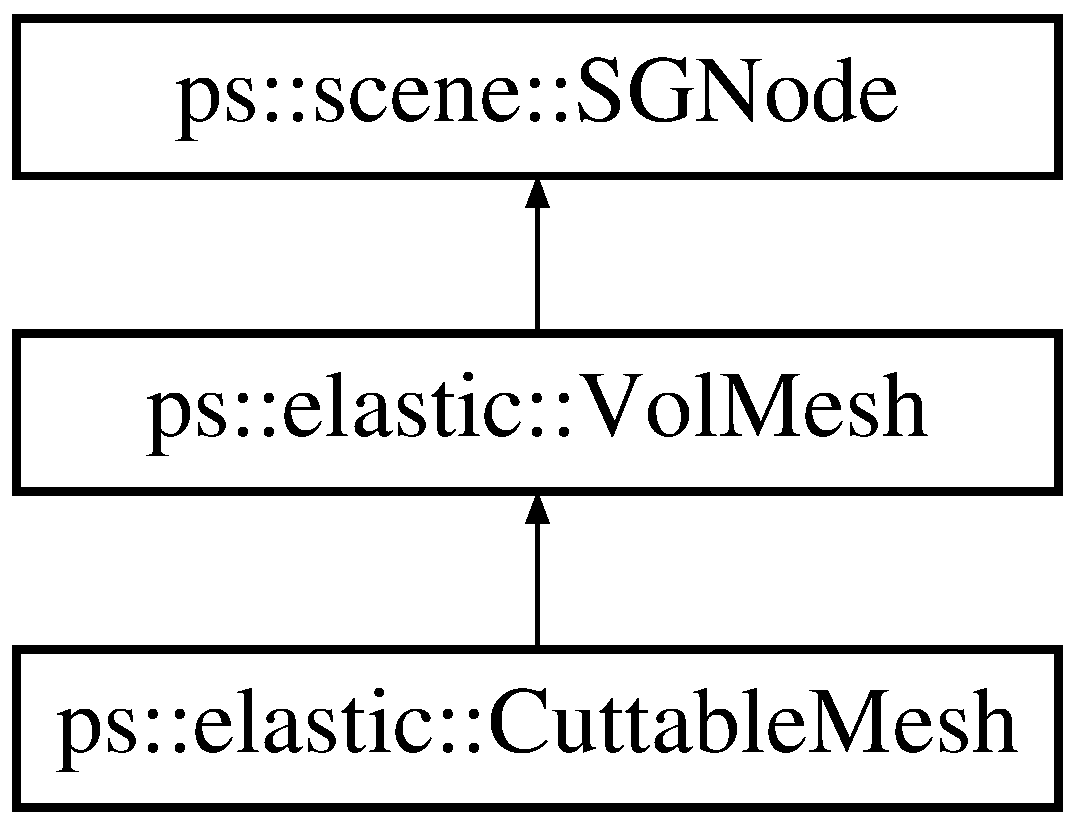
\includegraphics[height=3.000000cm]{classps_1_1elastic_1_1CuttableMesh}
\end{center}
\end{figure}
\subsection*{Classes}
\begin{DoxyCompactItemize}
\item 
class \hyperlink{classps_1_1elastic_1_1CuttableMesh_1_1CutEdge}{Cut\+Edge}
\item 
struct \hyperlink{structps_1_1elastic_1_1CuttableMesh_1_1CutNode}{Cut\+Node}
\end{DoxyCompactItemize}
\subsection*{Public Member Functions}
\begin{DoxyCompactItemize}
\item 
\hypertarget{classps_1_1elastic_1_1CuttableMesh_a1050ce8dfd09564ecd252c386d4c7743}{}{\bfseries Cuttable\+Mesh} (const \hyperlink{classps_1_1elastic_1_1VolMesh}{Vol\+Mesh} \&volmesh)\label{classps_1_1elastic_1_1CuttableMesh_a1050ce8dfd09564ecd252c386d4c7743}

\item 
\hypertarget{classps_1_1elastic_1_1CuttableMesh_a1245acf5e570ead2e0835594721d4adc}{}{\bfseries Cuttable\+Mesh} (const vector$<$ double $>$ \&vertices, const vector$<$ U32 $>$ \&elements)\label{classps_1_1elastic_1_1CuttableMesh_a1245acf5e570ead2e0835594721d4adc}

\item 
\hypertarget{classps_1_1elastic_1_1CuttableMesh_a8e01b70f0d11e393059dbda36645b755}{}{\bfseries Cuttable\+Mesh} (int ct\+Vertices, double $\ast$vertices, int ct\+Elements, int $\ast$elements)\label{classps_1_1elastic_1_1CuttableMesh_a8e01b70f0d11e393059dbda36645b755}

\item 
\hypertarget{classps_1_1elastic_1_1CuttableMesh_a933970175879dd15ac7e245e2c60a828}{}double {\bfseries point\+Line\+Distance} (const \hyperlink{classps_1_1base_1_1Vec3}{vec3d} \&v1, const \hyperlink{classps_1_1base_1_1Vec3}{vec3d} \&v2, const \hyperlink{classps_1_1base_1_1Vec3}{vec3d} \&p)\label{classps_1_1elastic_1_1CuttableMesh_a933970175879dd15ac7e245e2c60a828}

\item 
\hypertarget{classps_1_1elastic_1_1CuttableMesh_a22537bb36d06e7c7a57b56c8f2ec6177}{}double {\bfseries point\+Line\+Distance} (const \hyperlink{classps_1_1base_1_1Vec3}{vec3d} \&v1, const \hyperlink{classps_1_1base_1_1Vec3}{vec3d} \&v2, const double len2, const \hyperlink{classps_1_1base_1_1Vec3}{vec3d} \&p, double $\ast$out\+T=N\+U\+L\+L)\label{classps_1_1elastic_1_1CuttableMesh_a22537bb36d06e7c7a57b56c8f2ec6177}

\item 
\hypertarget{classps_1_1elastic_1_1CuttableMesh_a4d82322a19f083f4fa253eb77e06a9b9}{}void {\bfseries draw} ()\label{classps_1_1elastic_1_1CuttableMesh_a4d82322a19f083f4fa253eb77e06a9b9}

\item 
\hypertarget{classps_1_1elastic_1_1CuttableMesh_aa51f70d1383624cf84a6c18b62a29259}{}void {\bfseries sync\+Render} ()\label{classps_1_1elastic_1_1CuttableMesh_aa51f70d1383624cf84a6c18b62a29259}

\item 
\hypertarget{classps_1_1elastic_1_1CuttableMesh_a62df92014b8773a00312cc7728bf7da2}{}void {\bfseries clear\+Cut\+Context} ()\label{classps_1_1elastic_1_1CuttableMesh_a62df92014b8773a00312cc7728bf7da2}

\item 
\hypertarget{classps_1_1elastic_1_1CuttableMesh_a399904005742c9dfdff7bb434ab9bf76}{}int {\bfseries compute\+Cut\+Edges\+Kernel} (const \hyperlink{classps_1_1base_1_1Vec3}{vec3d} sweptquad\mbox{[}4\mbox{]}, std\+::map$<$ U32, \hyperlink{classps_1_1elastic_1_1CuttableMesh_1_1CutEdge}{Cut\+Edge} $>$ \&map\+Cut\+Edges)\label{classps_1_1elastic_1_1CuttableMesh_a399904005742c9dfdff7bb434ab9bf76}

\item 
\hypertarget{classps_1_1elastic_1_1CuttableMesh_add23a02582a31568808e6b652f542213}{}int {\bfseries compute\+Cut\+Nodes\+Kernel} (const \hyperlink{classps_1_1base_1_1Vec3}{vec3d} \&blade0, const \hyperlink{classps_1_1base_1_1Vec3}{vec3d} \&blade1, const \hyperlink{classps_1_1base_1_1Vec3}{vec3d} sweptquad\mbox{[}4\mbox{]}, std\+::map$<$ U32, \hyperlink{classps_1_1elastic_1_1CuttableMesh_1_1CutEdge}{Cut\+Edge} $>$ \&map\+Cut\+Edges, std\+::map$<$ U32, \hyperlink{structps_1_1elastic_1_1CuttableMesh_1_1CutNode}{Cut\+Node} $>$ \&map\+Cut\+Nodes)\label{classps_1_1elastic_1_1CuttableMesh_add23a02582a31568808e6b652f542213}

\item 
\hypertarget{classps_1_1elastic_1_1CuttableMesh_a4d77e2e597d0a625f999d15a269158c3}{}int {\bfseries cut} (const vector$<$ \hyperlink{classps_1_1base_1_1Vec3}{vec3d} $>$ \&segments, const vector$<$ \hyperlink{classps_1_1base_1_1Vec3}{vec3d} $>$ \&quadstrips, bool modify\+Mesh)\label{classps_1_1elastic_1_1CuttableMesh_a4d77e2e597d0a625f999d15a269158c3}

\item 
\hypertarget{classps_1_1elastic_1_1CuttableMesh_a8a8b7a44f8248de22a90deb4c8960962}{}\hyperlink{classps_1_1base_1_1Vec3}{vec3d} {\bfseries vertex\+Rest\+Pos\+At} (U32 i) const \label{classps_1_1elastic_1_1CuttableMesh_a8a8b7a44f8248de22a90deb4c8960962}

\item 
\hypertarget{classps_1_1elastic_1_1CuttableMesh_a684f7b36a4e5fb9846099fd8995caa38}{}int {\bfseries find\+Closest\+Vertex} (const \hyperlink{classps_1_1base_1_1Vec3}{vec3d} \&query, double \&dist, \hyperlink{classps_1_1base_1_1Vec3}{vec3d} \&out\+P) const \label{classps_1_1elastic_1_1CuttableMesh_a684f7b36a4e5fb9846099fd8995caa38}

\item 
\hypertarget{classps_1_1elastic_1_1CuttableMesh_aabb3fc0ca125b096110914671d7ced5d}{}int {\bfseries count\+Completed\+Cuts} () const \label{classps_1_1elastic_1_1CuttableMesh_aabb3fc0ca125b096110914671d7ced5d}

\item 
\hypertarget{classps_1_1elastic_1_1CuttableMesh_aaf49f2d8cbbaf485f6a1bcb72d00e609}{}\hyperlink{classps_1_1elastic_1_1TetSubdivider}{Tet\+Subdivider} $\ast$ {\bfseries get\+Sub\+D} () const \label{classps_1_1elastic_1_1CuttableMesh_aaf49f2d8cbbaf485f6a1bcb72d00e609}

\item 
bool \hyperlink{classps_1_1elastic_1_1CuttableMesh_a786edd24a931fe37af887798ce203916}{split\+Parts} (const \hyperlink{classps_1_1base_1_1Vec3}{vec3d} sweptquad\mbox{[}4\mbox{]}, double dist)
\item 
int \hyperlink{classps_1_1elastic_1_1CuttableMesh_a6669524e92d7a5c2784fefaa4f51d1a5}{convert\+Disjoint\+Parts\+To\+Meshes} (vector$<$ \hyperlink{classps_1_1elastic_1_1CuttableMesh}{Cuttable\+Mesh} $\ast$ $>$ \&v\+Out\+New\+Meshes)
\item 
void \hyperlink{classps_1_1elastic_1_1CuttableMesh_aee7462902722caff22b8ff0ea0ec8478}{apply\+Transform\+To\+Mesh\+Then\+Reset\+Transform} ()
\item 
\hypertarget{classps_1_1elastic_1_1CuttableMesh_a2eaa09e7afaf6c4e07cb186207124812}{}bool {\bfseries get\+Flag\+Split\+Mesh\+After\+Cut} () const \label{classps_1_1elastic_1_1CuttableMesh_a2eaa09e7afaf6c4e07cb186207124812}

\item 
\hypertarget{classps_1_1elastic_1_1CuttableMesh_a2893f36d95f74ba71800fffc36c18112}{}void {\bfseries set\+Flag\+Split\+Mesh\+After\+Cut} (bool flag)\label{classps_1_1elastic_1_1CuttableMesh_a2893f36d95f74ba71800fffc36c18112}

\item 
\hypertarget{classps_1_1elastic_1_1CuttableMesh_a32667014d30499be73e3ec1d2f9eba95}{}bool {\bfseries get\+Flag\+Detect\+Cut\+Nodes} () const \label{classps_1_1elastic_1_1CuttableMesh_a32667014d30499be73e3ec1d2f9eba95}

\item 
\hypertarget{classps_1_1elastic_1_1CuttableMesh_a6370f263fd60001ae4ca462187fc2df8}{}void {\bfseries set\+Flag\+Detect\+Cut\+Nodes} (bool flag)\label{classps_1_1elastic_1_1CuttableMesh_a6370f263fd60001ae4ca462187fc2df8}

\item 
\hypertarget{classps_1_1elastic_1_1CuttableMesh_afceffb1e083b60deede3bf263da982d5}{}bool {\bfseries get\+Flag\+Draw\+Sweep\+Surf} () const \label{classps_1_1elastic_1_1CuttableMesh_afceffb1e083b60deede3bf263da982d5}

\item 
\hypertarget{classps_1_1elastic_1_1CuttableMesh_a9da5ceded5ef7f2ecffb80f20a45dfa3}{}void {\bfseries set\+Flag\+Draw\+Sweep\+Surf} (bool flag)\label{classps_1_1elastic_1_1CuttableMesh_a9da5ceded5ef7f2ecffb80f20a45dfa3}

\item 
\hypertarget{classps_1_1elastic_1_1CuttableMesh_af8d9bfb7d00d9485c2f38a06aa768113}{}bool {\bfseries get\+Flag\+Draw\+A\+A\+B\+B} () const \label{classps_1_1elastic_1_1CuttableMesh_af8d9bfb7d00d9485c2f38a06aa768113}

\item 
\hypertarget{classps_1_1elastic_1_1CuttableMesh_abcdcebec31e9a88d2732e7e8f5cc32b7}{}void {\bfseries set\+Flag\+Draw\+A\+A\+B\+B} (bool flag)\label{classps_1_1elastic_1_1CuttableMesh_abcdcebec31e9a88d2732e7e8f5cc32b7}

\end{DoxyCompactItemize}
\subsection*{Protected Member Functions}
\begin{DoxyCompactItemize}
\item 
\hypertarget{classps_1_1elastic_1_1CuttableMesh_a00ee3e65bff52a11ec74d8a65db2adcb}{}void {\bfseries setup} ()\label{classps_1_1elastic_1_1CuttableMesh_a00ee3e65bff52a11ec74d8a65db2adcb}

\end{DoxyCompactItemize}
\subsection*{Additional Inherited Members}


\subsection{Member Function Documentation}
\hypertarget{classps_1_1elastic_1_1CuttableMesh_aee7462902722caff22b8ff0ea0ec8478}{}\index{ps\+::elastic\+::\+Cuttable\+Mesh@{ps\+::elastic\+::\+Cuttable\+Mesh}!apply\+Transform\+To\+Mesh\+Then\+Reset\+Transform@{apply\+Transform\+To\+Mesh\+Then\+Reset\+Transform}}
\index{apply\+Transform\+To\+Mesh\+Then\+Reset\+Transform@{apply\+Transform\+To\+Mesh\+Then\+Reset\+Transform}!ps\+::elastic\+::\+Cuttable\+Mesh@{ps\+::elastic\+::\+Cuttable\+Mesh}}
\subsubsection[{apply\+Transform\+To\+Mesh\+Then\+Reset\+Transform()}]{\setlength{\rightskip}{0pt plus 5cm}void ps\+::elastic\+::\+Cuttable\+Mesh\+::apply\+Transform\+To\+Mesh\+Then\+Reset\+Transform (
\begin{DoxyParamCaption}
{}
\end{DoxyParamCaption}
)}\label{classps_1_1elastic_1_1CuttableMesh_aee7462902722caff22b8ff0ea0ec8478}
This is a convenient function to aid in transforming original volume meshes and placing them in the right projection view. Later the transform is applied to all mesh nodes and then the transform itself is reset. \hypertarget{classps_1_1elastic_1_1CuttableMesh_a6669524e92d7a5c2784fefaa4f51d1a5}{}\index{ps\+::elastic\+::\+Cuttable\+Mesh@{ps\+::elastic\+::\+Cuttable\+Mesh}!convert\+Disjoint\+Parts\+To\+Meshes@{convert\+Disjoint\+Parts\+To\+Meshes}}
\index{convert\+Disjoint\+Parts\+To\+Meshes@{convert\+Disjoint\+Parts\+To\+Meshes}!ps\+::elastic\+::\+Cuttable\+Mesh@{ps\+::elastic\+::\+Cuttable\+Mesh}}
\subsubsection[{convert\+Disjoint\+Parts\+To\+Meshes(vector$<$ Cuttable\+Mesh $\ast$ $>$ \&v\+Out\+New\+Meshes)}]{\setlength{\rightskip}{0pt plus 5cm}int ps\+::elastic\+::\+Cuttable\+Mesh\+::convert\+Disjoint\+Parts\+To\+Meshes (
\begin{DoxyParamCaption}
\item[{vector$<$ {\bf Cuttable\+Mesh} $\ast$ $>$ \&}]{v\+Out\+New\+Meshes}
\end{DoxyParamCaption}
)}\label{classps_1_1elastic_1_1CuttableMesh_a6669524e92d7a5c2784fefaa4f51d1a5}
First finds all disjoint parts of the mesh and then produces new cuttablemesh nodes out of those disjoint pieces. Main mesh will be part of the newly created meshes so the original cuttable mesh node can be discarded if desired. 
\begin{DoxyParams}{Parameters}
{\em v\+Out\+New\+Meshes} & list of newly created mesh nodes \\
\hline
\end{DoxyParams}
\begin{DoxyReturn}{Returns}
number of newly created mesh nodes. 
\end{DoxyReturn}
\hypertarget{classps_1_1elastic_1_1CuttableMesh_a786edd24a931fe37af887798ce203916}{}\index{ps\+::elastic\+::\+Cuttable\+Mesh@{ps\+::elastic\+::\+Cuttable\+Mesh}!split\+Parts@{split\+Parts}}
\index{split\+Parts@{split\+Parts}!ps\+::elastic\+::\+Cuttable\+Mesh@{ps\+::elastic\+::\+Cuttable\+Mesh}}
\subsubsection[{split\+Parts(const vec3d sweptquad[4], double dist)}]{\setlength{\rightskip}{0pt plus 5cm}bool ps\+::elastic\+::\+Cuttable\+Mesh\+::split\+Parts (
\begin{DoxyParamCaption}
\item[{const {\bf vec3d}}]{sweptquad\mbox{[}4\mbox{]}, }
\item[{double}]{dist}
\end{DoxyParamCaption}
)}\label{classps_1_1elastic_1_1CuttableMesh_a786edd24a931fe37af887798ce203916}
splits the mesh parts using the sweep surface. 
\begin{DoxyParams}{Parameters}
{\em v\+Sweept\+Surf} & \\
\hline
{\em dist} & \\
\hline
\end{DoxyParams}
\begin{DoxyReturn}{Returns}

\end{DoxyReturn}


The documentation for this class was generated from the following files\+:\begin{DoxyCompactItemize}
\item 
/\+Users/pourya/\+Desktop/platform/repos/tetcutter/src/elastic/cuttablemesh.\+h\item 
/\+Users/pourya/\+Desktop/platform/repos/tetcutter/src/elastic/cuttablemesh.\+cpp\end{DoxyCompactItemize}

\hypertarget{classps_1_1base_1_1CWString}{}\section{ps\+:\+:base\+:\+:C\+W\+String Class Reference}
\label{classps_1_1base_1_1CWString}\index{ps\+::base\+::\+C\+W\+String@{ps\+::base\+::\+C\+W\+String}}
Inheritance diagram for ps\+:\+:base\+:\+:C\+W\+String\+:\begin{figure}[H]
\begin{center}
\leavevmode
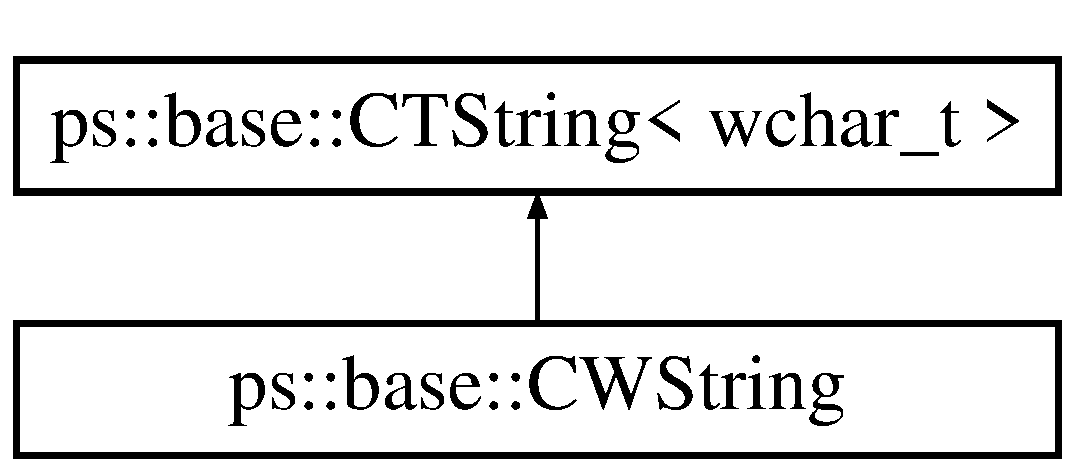
\includegraphics[height=2.000000cm]{classps_1_1base_1_1CWString}
\end{center}
\end{figure}
\subsection*{Public Types}
\begin{DoxyCompactItemize}
\item 
\hypertarget{classps_1_1base_1_1CWString_a7a6d143e2b52a26407e6c561e9a056a5}{}typedef wchar\+\_\+t {\bfseries U\+N\+I\+T}\label{classps_1_1base_1_1CWString_a7a6d143e2b52a26407e6c561e9a056a5}

\end{DoxyCompactItemize}
\subsection*{Public Member Functions}
\begin{DoxyCompactItemize}
\item 
\hypertarget{classps_1_1base_1_1CWString_afa718ed783ec810c4e4ae1c200cecedb}{}{\bfseries C\+W\+String} (const char src\mbox{[}$\,$\mbox{]}, int src\+Size=0)\label{classps_1_1base_1_1CWString_afa718ed783ec810c4e4ae1c200cecedb}

\item 
\hypertarget{classps_1_1base_1_1CWString_adc731938a7f972a5e474ee8ae123afc6}{}{\bfseries C\+W\+String} (const wchar\+\_\+t src\mbox{[}$\,$\mbox{]}, int src\+Size=0)\label{classps_1_1base_1_1CWString_adc731938a7f972a5e474ee8ae123afc6}

\item 
\hypertarget{classps_1_1base_1_1CWString_a83cac3f3f5687b4bc9b3d7b7c2237f50}{}{\bfseries C\+W\+String} (const \hyperlink{classps_1_1base_1_1CWString}{C\+W\+String} \&src)\label{classps_1_1base_1_1CWString_a83cac3f3f5687b4bc9b3d7b7c2237f50}

\item 
\hypertarget{classps_1_1base_1_1CWString_a868835a8bf516e3aa70061733d298fe8}{}int {\bfseries get\+Input\+Length} (const wchar\+\_\+t src\mbox{[}$\,$\mbox{]}) const \label{classps_1_1base_1_1CWString_a868835a8bf516e3aa70061733d298fe8}

\item 
\hypertarget{classps_1_1base_1_1CWString_a70033f3a0d59e3046a1051f4e0f8d8c3}{}void {\bfseries copy\+From\+A} (const char src\mbox{[}$\,$\mbox{]}, int src\+Size=0)\label{classps_1_1base_1_1CWString_a70033f3a0d59e3046a1051f4e0f8d8c3}

\item 
\hypertarget{classps_1_1base_1_1CWString_a023b535126e6e3e599e844084405dfb7}{}void {\bfseries append\+From\+A} (const char src\mbox{[}$\,$\mbox{]}, int src\+Size=0)\label{classps_1_1base_1_1CWString_a023b535126e6e3e599e844084405dfb7}

\item 
\hypertarget{classps_1_1base_1_1CWString_aab4a3437ad012fffc8ff72e0683c2363}{}void {\bfseries append\+From\+A} (const char ch)\label{classps_1_1base_1_1CWString_aab4a3437ad012fffc8ff72e0683c2363}

\item 
\hypertarget{classps_1_1base_1_1CWString_a663becbe8fc2d7633de35d38cf957f2a}{}\hyperlink{classps_1_1base_1_1CWString}{C\+W\+String} {\bfseries substr} (int offset, int count=-\/1) const \label{classps_1_1base_1_1CWString_a663becbe8fc2d7633de35d38cf957f2a}

\item 
\hypertarget{classps_1_1base_1_1CWString_a1b8670512b59e8d4b036a2c393afb1e7}{}\hyperlink{classps_1_1base_1_1CWString}{C\+W\+String} \& {\bfseries to\+Upper} ()\label{classps_1_1base_1_1CWString_a1b8670512b59e8d4b036a2c393afb1e7}

\item 
\hypertarget{classps_1_1base_1_1CWString_abb8b66c5cecb7a675e696909113f9c2e}{}\hyperlink{classps_1_1base_1_1CWString}{C\+W\+String} \& {\bfseries to\+Lower} ()\label{classps_1_1base_1_1CWString_abb8b66c5cecb7a675e696909113f9c2e}

\item 
\hypertarget{classps_1_1base_1_1CWString_a93f55d9f61f1ec86bbd85eb53a6e1bf5}{}\hyperlink{classps_1_1base_1_1CWString}{C\+W\+String} {\bfseries operator+} (const \hyperlink{classps_1_1base_1_1CWString}{C\+W\+String} \&src) const \label{classps_1_1base_1_1CWString_a93f55d9f61f1ec86bbd85eb53a6e1bf5}

\item 
\hypertarget{classps_1_1base_1_1CWString_af66d8ddc70c99b07bab2e597dcc9df58}{}\hyperlink{classps_1_1base_1_1CWString}{C\+W\+String} {\bfseries operator+} (const wchar\+\_\+t src\mbox{[}$\,$\mbox{]}) const \label{classps_1_1base_1_1CWString_af66d8ddc70c99b07bab2e597dcc9df58}

\item 
\hypertarget{classps_1_1base_1_1CWString_a52b7ce55e3bf318089f64a419ac36350}{}\hyperlink{classps_1_1base_1_1CWString}{C\+W\+String} {\bfseries operator+} (wchar\+\_\+t src\mbox{[}$\,$\mbox{]}) const \label{classps_1_1base_1_1CWString_a52b7ce55e3bf318089f64a419ac36350}

\item 
\hypertarget{classps_1_1base_1_1CWString_a689071dbf3f4d1873dfe118cebc5fff6}{}\hyperlink{classps_1_1base_1_1CWString}{C\+W\+String} {\bfseries operator+} (const char src\mbox{[}$\,$\mbox{]}) const \label{classps_1_1base_1_1CWString_a689071dbf3f4d1873dfe118cebc5fff6}

\item 
\hypertarget{classps_1_1base_1_1CWString_a631df8233db281eefc19196b5405eb87}{}\hyperlink{classps_1_1base_1_1CWString}{C\+W\+String} {\bfseries operator+} (char src\mbox{[}$\,$\mbox{]}) const \label{classps_1_1base_1_1CWString_a631df8233db281eefc19196b5405eb87}

\item 
\hypertarget{classps_1_1base_1_1CWString_a91b0626f816ddd8e495bcc96151c3fa9}{}\hyperlink{classps_1_1base_1_1CWString}{C\+W\+String} {\bfseries operator+} (const char ch) const \label{classps_1_1base_1_1CWString_a91b0626f816ddd8e495bcc96151c3fa9}

\item 
\hypertarget{classps_1_1base_1_1CWString_ae75302136b8fea8c567634bb92698693}{}\hyperlink{classps_1_1base_1_1CWString}{C\+W\+String} {\bfseries operator+} (const wchar\+\_\+t ch) const \label{classps_1_1base_1_1CWString_ae75302136b8fea8c567634bb92698693}

\item 
\hypertarget{classps_1_1base_1_1CWString_a83910d44c6c5ec177ea16d65574fe228}{}void {\bfseries operator+=} (const \hyperlink{classps_1_1base_1_1CWString}{C\+W\+String} \&src)\label{classps_1_1base_1_1CWString_a83910d44c6c5ec177ea16d65574fe228}

\item 
\hypertarget{classps_1_1base_1_1CWString_a14dc2ebc1a128bc67481a8b128176e32}{}void {\bfseries operator+=} (const wchar\+\_\+t src\mbox{[}$\,$\mbox{]})\label{classps_1_1base_1_1CWString_a14dc2ebc1a128bc67481a8b128176e32}

\item 
\hypertarget{classps_1_1base_1_1CWString_aea1c10e9d32c81c17a77d9646b32f21b}{}void {\bfseries operator+=} (wchar\+\_\+t src\mbox{[}$\,$\mbox{]})\label{classps_1_1base_1_1CWString_aea1c10e9d32c81c17a77d9646b32f21b}

\item 
\hypertarget{classps_1_1base_1_1CWString_a63fe1db878c79b36119aef7cc35917ae}{}void {\bfseries operator+=} (const char src\mbox{[}$\,$\mbox{]})\label{classps_1_1base_1_1CWString_a63fe1db878c79b36119aef7cc35917ae}

\item 
\hypertarget{classps_1_1base_1_1CWString_a6cc27d171e076de29db977fbf252a18e}{}void {\bfseries operator+=} (char src\mbox{[}$\,$\mbox{]})\label{classps_1_1base_1_1CWString_a6cc27d171e076de29db977fbf252a18e}

\item 
\hypertarget{classps_1_1base_1_1CWString_a01d28ad2a2773e515f4d1f8630023fb9}{}void {\bfseries operator+=} (const char ch)\label{classps_1_1base_1_1CWString_a01d28ad2a2773e515f4d1f8630023fb9}

\item 
\hypertarget{classps_1_1base_1_1CWString_a4f639b76f3c02e3c218974a2d26f173c}{}void {\bfseries operator+=} (const wchar\+\_\+t ch)\label{classps_1_1base_1_1CWString_a4f639b76f3c02e3c218974a2d26f173c}

\item 
\hypertarget{classps_1_1base_1_1CWString_a7d910fd675a50235942923da9f5b1420}{}void {\bfseries operator=} (const char src\mbox{[}$\,$\mbox{]})\label{classps_1_1base_1_1CWString_a7d910fd675a50235942923da9f5b1420}

\item 
\hypertarget{classps_1_1base_1_1CWString_a229be1b24fa5cc1cc3094e961f926f3e}{}void {\bfseries operator=} (const wchar\+\_\+t src\mbox{[}$\,$\mbox{]})\label{classps_1_1base_1_1CWString_a229be1b24fa5cc1cc3094e961f926f3e}

\end{DoxyCompactItemize}
\subsection*{Friends}
\begin{DoxyCompactItemize}
\item 
\hypertarget{classps_1_1base_1_1CWString_a088804404b2bd2cc784eb7efab6e8352}{}bool {\bfseries operator==} (const \hyperlink{classps_1_1base_1_1CWString}{C\+W\+String} \&a, const \hyperlink{classps_1_1base_1_1CWString}{C\+W\+String} \&b)\label{classps_1_1base_1_1CWString_a088804404b2bd2cc784eb7efab6e8352}

\item 
\hypertarget{classps_1_1base_1_1CWString_a4b138b6163fa871754420174beaceafe}{}bool {\bfseries operator!=} (const \hyperlink{classps_1_1base_1_1CWString}{C\+W\+String} \&a, const \hyperlink{classps_1_1base_1_1CWString}{C\+W\+String} \&b)\label{classps_1_1base_1_1CWString_a4b138b6163fa871754420174beaceafe}

\item 
\hypertarget{classps_1_1base_1_1CWString_a6270ea1b8ae876bceffcece540cfc43a}{}std\+::ostream \& {\bfseries operator$<$$<$} (std\+::ostream \&outs, const \hyperlink{classps_1_1base_1_1CWString}{C\+W\+String} \&src)\label{classps_1_1base_1_1CWString_a6270ea1b8ae876bceffcece540cfc43a}

\item 
\hypertarget{classps_1_1base_1_1CWString_acabf840c60b48242da8d70df900f393d}{}std\+::istream \& {\bfseries operator$>$$>$} (std\+::istream \&ins, \hyperlink{classps_1_1base_1_1CWString}{C\+W\+String} \&src)\label{classps_1_1base_1_1CWString_acabf840c60b48242da8d70df900f393d}

\end{DoxyCompactItemize}
\subsection*{Additional Inherited Members}


The documentation for this class was generated from the following files\+:\begin{DoxyCompactItemize}
\item 
/\+Users/pourya/\+Desktop/platform/repos/tetcutter/src/base/str.\+h\item 
/\+Users/pourya/\+Desktop/platform/repos/tetcutter/src/base/str.\+cpp\end{DoxyCompactItemize}

\hypertarget{classps_1_1elastic_1_1EDGE}{}\section{ps\+:\+:elastic\+:\+:E\+D\+G\+E Class Reference}
\label{classps_1_1elastic_1_1EDGE}\index{ps\+::elastic\+::\+E\+D\+G\+E@{ps\+::elastic\+::\+E\+D\+G\+E}}
\subsection*{Public Member Functions}
\begin{DoxyCompactItemize}
\item 
\hypertarget{classps_1_1elastic_1_1EDGE_a7a17a2d3e5d307164a5e4ace0705a3ce}{}{\bfseries E\+D\+G\+E} (U32 from\+\_\+, U32 to\+\_\+)\label{classps_1_1elastic_1_1EDGE_a7a17a2d3e5d307164a5e4ace0705a3ce}

\item 
\hypertarget{classps_1_1elastic_1_1EDGE_a7c8d8f8da508cea1a05bb529b42c1467}{}void {\bfseries init} ()\label{classps_1_1elastic_1_1EDGE_a7c8d8f8da508cea1a05bb529b42c1467}

\item 
\hypertarget{classps_1_1elastic_1_1EDGE_aaad75706e275d2161084c72d5b87ee9f}{}void {\bfseries setup} (U32 from\+\_\+, U32 to\+\_\+)\label{classps_1_1elastic_1_1EDGE_aaad75706e275d2161084c72d5b87ee9f}

\item 
\hypertarget{classps_1_1elastic_1_1EDGE_a6db7916e4af6523ebdb74f32f9edc943}{}\hyperlink{classps_1_1elastic_1_1EDGE}{E\+D\+G\+E} \& {\bfseries operator=} (const \hyperlink{classps_1_1elastic_1_1EDGE}{E\+D\+G\+E} \&A)\label{classps_1_1elastic_1_1EDGE_a6db7916e4af6523ebdb74f32f9edc943}

\end{DoxyCompactItemize}
\subsection*{Public Attributes}
\begin{DoxyCompactItemize}
\item 
\hypertarget{classps_1_1elastic_1_1EDGE_a7879567b21f23c188bc9915d04b1015d}{}U32 {\bfseries from}\label{classps_1_1elastic_1_1EDGE_a7879567b21f23c188bc9915d04b1015d}

\item 
\hypertarget{classps_1_1elastic_1_1EDGE_accd00008f498d0110a35df7152203db6}{}U32 {\bfseries to}\label{classps_1_1elastic_1_1EDGE_accd00008f498d0110a35df7152203db6}

\end{DoxyCompactItemize}


The documentation for this class was generated from the following file\+:\begin{DoxyCompactItemize}
\item 
/\+Users/pourya/\+Desktop/platform/repos/tetcutter/src/elastic/volmeshentities.\+h\end{DoxyCompactItemize}

\hypertarget{classps_1_1elastic_1_1EdgeKey}{}\section{ps\+:\+:elastic\+:\+:Edge\+Key Class Reference}
\label{classps_1_1elastic_1_1EdgeKey}\index{ps\+::elastic\+::\+Edge\+Key@{ps\+::elastic\+::\+Edge\+Key}}
\subsection*{Public Member Functions}
\begin{DoxyCompactItemize}
\item 
\hypertarget{classps_1_1elastic_1_1EdgeKey_aa306aadbf06a81494997ad2c846c20bd}{}{\bfseries Edge\+Key} (U64 k)\label{classps_1_1elastic_1_1EdgeKey_aa306aadbf06a81494997ad2c846c20bd}

\item 
\hypertarget{classps_1_1elastic_1_1EdgeKey_a5d7a226868ee9637f6c54d68508a5e14}{}{\bfseries Edge\+Key} (U32 a, U32 b)\label{classps_1_1elastic_1_1EdgeKey_a5d7a226868ee9637f6c54d68508a5e14}

\item 
\hypertarget{classps_1_1elastic_1_1EdgeKey_af900469a871dba24107eda8188e3cb85}{}void {\bfseries setup} (U32 a, U32 b)\label{classps_1_1elastic_1_1EdgeKey_af900469a871dba24107eda8188e3cb85}

\item 
\hypertarget{classps_1_1elastic_1_1EdgeKey_af29e66108acfd35c32616d429d80841d}{}bool {\bfseries operator$<$} (const \hyperlink{classps_1_1elastic_1_1EdgeKey}{Edge\+Key} \&k) const \label{classps_1_1elastic_1_1EdgeKey_af29e66108acfd35c32616d429d80841d}

\item 
\hypertarget{classps_1_1elastic_1_1EdgeKey_a7692060e4041ec2eed78cbd5e3574dcf}{}bool {\bfseries operator$>$} (const \hyperlink{classps_1_1elastic_1_1EdgeKey}{Edge\+Key} \&k) const \label{classps_1_1elastic_1_1EdgeKey_a7692060e4041ec2eed78cbd5e3574dcf}

\item 
\hypertarget{classps_1_1elastic_1_1EdgeKey_aa7d2dd8d6c3363fa73c969e22dfc68b0}{}void {\bfseries operator=} (const \hyperlink{classps_1_1elastic_1_1EdgeKey}{Edge\+Key} \&other)\label{classps_1_1elastic_1_1EdgeKey_aa7d2dd8d6c3363fa73c969e22dfc68b0}

\end{DoxyCompactItemize}
\subsection*{Public Attributes}
\begin{DoxyCompactItemize}
\item 
\hypertarget{classps_1_1elastic_1_1EdgeKey_a240ecee3a3243bb9b227119169865cb9}{}U64 {\bfseries key}\label{classps_1_1elastic_1_1EdgeKey_a240ecee3a3243bb9b227119169865cb9}

\end{DoxyCompactItemize}


The documentation for this class was generated from the following file\+:\begin{DoxyCompactItemize}
\item 
/\+Users/pourya/\+Desktop/platform/repos/tetcutter/src/elastic/volmeshentities.\+h\end{DoxyCompactItemize}

\hypertarget{classps_1_1elastic_1_1EdgeLink}{}\section{ps\+:\+:elastic\+:\+:Edge\+Link Class Reference}
\label{classps_1_1elastic_1_1EdgeLink}\index{ps\+::elastic\+::\+Edge\+Link@{ps\+::elastic\+::\+Edge\+Link}}
Inheritance diagram for ps\+:\+:elastic\+:\+:Edge\+Link\+:\begin{figure}[H]
\begin{center}
\leavevmode
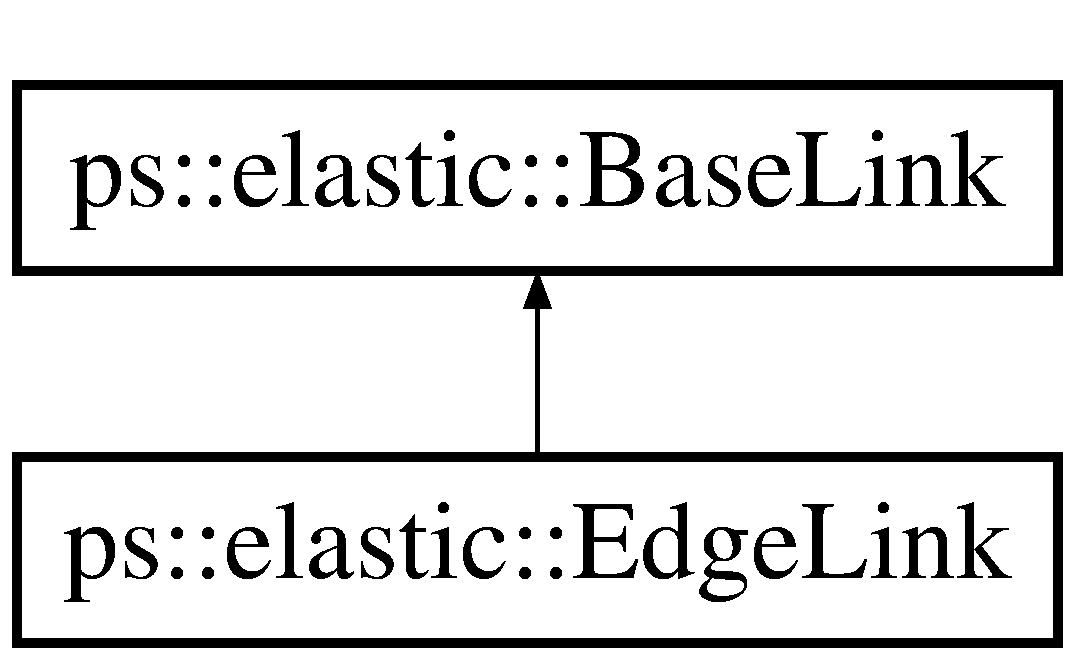
\includegraphics[height=2.000000cm]{classps_1_1elastic_1_1EdgeLink}
\end{center}
\end{figure}
\subsection*{Static Public Member Functions}
\begin{DoxyCompactItemize}
\item 
\hypertarget{classps_1_1elastic_1_1EdgeLink_ab58b42b0aa4cfcf6269e549d57f9caf1}{}static \hyperlink{classps_1_1elastic_1_1EdgeLink}{Edge\+Link} {\bfseries create} (U32 idx)\label{classps_1_1elastic_1_1EdgeLink_ab58b42b0aa4cfcf6269e549d57f9caf1}

\end{DoxyCompactItemize}
\subsection*{Additional Inherited Members}


The documentation for this class was generated from the following file\+:\begin{DoxyCompactItemize}
\item 
/\+Users/pourya/\+Desktop/platform/repos/tetcutter/src/elastic/volmeshentities.\+h\end{DoxyCompactItemize}

\hypertarget{structps_1_1utils_1_1EventLogger_1_1Event}{}\section{ps\+:\+:utils\+:\+:Event\+Logger\+:\+:Event Struct Reference}
\label{structps_1_1utils_1_1EventLogger_1_1Event}\index{ps\+::utils\+::\+Event\+Logger\+::\+Event@{ps\+::utils\+::\+Event\+Logger\+::\+Event}}
\subsection*{Public Attributes}
\begin{DoxyCompactItemize}
\item 
\hypertarget{structps_1_1utils_1_1EventLogger_1_1Event_abd567d95cdef3c2d7d1582e32604beff}{}Event\+Logger\+::\+E\+V\+E\+N\+T\+T\+Y\+P\+E {\bfseries etype}\label{structps_1_1utils_1_1EventLogger_1_1Event_abd567d95cdef3c2d7d1582e32604beff}

\item 
\hypertarget{structps_1_1utils_1_1EventLogger_1_1Event_a2492f5382f17bceb58d0a3f0526bd856}{}\hyperlink{classps_1_1base_1_1CAString}{Ansi\+Str} {\bfseries str\+Desc}\label{structps_1_1utils_1_1EventLogger_1_1Event_a2492f5382f17bceb58d0a3f0526bd856}

\item 
\hypertarget{structps_1_1utils_1_1EventLogger_1_1Event_aff09bc1a51cf30196c5de540eaa138b2}{}\hyperlink{classps_1_1base_1_1CAString}{Ansi\+Str} {\bfseries str\+Source}\label{structps_1_1utils_1_1EventLogger_1_1Event_aff09bc1a51cf30196c5de540eaa138b2}

\item 
\hypertarget{structps_1_1utils_1_1EventLogger_1_1Event_a99b03414776fc8b1ce2608279b900222}{}int {\bfseries value}\label{structps_1_1utils_1_1EventLogger_1_1Event_a99b03414776fc8b1ce2608279b900222}

\end{DoxyCompactItemize}


The documentation for this struct was generated from the following file\+:\begin{DoxyCompactItemize}
\item 
/\+Users/pourya/\+Desktop/platform/repos/tetcutter/src/base/Logger.\+h\end{DoxyCompactItemize}

\hypertarget{classps_1_1utils_1_1EventLogger}{}\section{ps\+:\+:utils\+:\+:Event\+Logger Class Reference}
\label{classps_1_1utils_1_1EventLogger}\index{ps\+::utils\+::\+Event\+Logger@{ps\+::utils\+::\+Event\+Logger}}


{\ttfamily \#include $<$logger.\+h$>$}

\subsection*{Classes}
\begin{DoxyCompactItemize}
\item 
struct \hyperlink{structps_1_1utils_1_1EventLogger_1_1Event}{Event}
\end{DoxyCompactItemize}
\subsection*{Public Types}
\begin{DoxyCompactItemize}
\item 
\hypertarget{classps_1_1utils_1_1EventLogger_a2ec7ed52f7fe7780454cfa214ecdc575}{}enum {\bfseries E\+V\+E\+N\+T\+T\+Y\+P\+E} \{ {\bfseries et\+Profile}, 
{\bfseries et\+Info}, 
{\bfseries et\+Warning}, 
{\bfseries et\+Error}
 \}\label{classps_1_1utils_1_1EventLogger_a2ec7ed52f7fe7780454cfa214ecdc575}

\end{DoxyCompactItemize}
\subsection*{Public Member Functions}
\begin{DoxyCompactItemize}
\item 
\hyperlink{classps_1_1utils_1_1EventLogger_a952c1d904e9dbe976bc80919413bdaa7}{Event\+Logger} (const char $\ast$lp\+File\+Path, int flags=0)
\item 
void \hyperlink{classps_1_1utils_1_1EventLogger_a408da0eba198ea67f4f5dd2cbad50a5b}{add} (const \hyperlink{structps_1_1utils_1_1EventLogger_1_1Event}{Event} \&e)
\item 
void \hyperlink{classps_1_1utils_1_1EventLogger_a1218f827938c74c78d96ab63f0a826a1}{add} (const char $\ast$lp\+Str\+Desc, E\+V\+E\+N\+T\+T\+Y\+P\+E t=et\+Info, const char $\ast$lp\+Str\+Source=N\+U\+L\+L, int value=0)
\item 
void \hyperlink{classps_1_1utils_1_1EventLogger_ac86c18aa6df7a5eb774d34d31dde0451}{set\+Write\+Flags} (int flags)
\item 
\hypertarget{classps_1_1utils_1_1EventLogger_a385bd436b0f21cbf11c7a554b9f0dcab}{}void {\bfseries set\+Out\+File\+Path} (const char $\ast$lp\+Str\+File\+Path)\label{classps_1_1utils_1_1EventLogger_a385bd436b0f21cbf11c7a554b9f0dcab}

\item 
\hypertarget{classps_1_1utils_1_1EventLogger_a0f6b79c708ee991dc18adbdd8aff6ffb}{}void {\bfseries set\+Display\+Call\+Back} (F\+On\+Display cb)\label{classps_1_1utils_1_1EventLogger_a0f6b79c708ee991dc18adbdd8aff6ffb}

\item 
\hypertarget{classps_1_1utils_1_1EventLogger_ab5f54fa75186ec718accd369bde4a138}{}bool {\bfseries flush} ()\label{classps_1_1utils_1_1EventLogger_ab5f54fa75186ec718accd369bde4a138}

\item 
\hypertarget{classps_1_1utils_1_1EventLogger_a38e7c4ad4cfe86133f0055481f4f1d77}{}\hyperlink{classps_1_1base_1_1CAString}{Ansi\+Str} {\bfseries root\+Path} () const \label{classps_1_1utils_1_1EventLogger_a38e7c4ad4cfe86133f0055481f4f1d77}

\item 
\hypertarget{classps_1_1utils_1_1EventLogger_ae39e90031c86daa9ab9dc1e5e6f0793a}{}\hyperlink{classps_1_1base_1_1CAString}{Ansi\+Str} {\bfseries shorten\+Path\+Based\+On\+Root} (const \hyperlink{classps_1_1base_1_1CAString}{Ansi\+Str} \&str\+Path) const \label{classps_1_1utils_1_1EventLogger_ae39e90031c86daa9ab9dc1e5e6f0793a}

\end{DoxyCompactItemize}


\subsection{Detailed Description}
\hyperlink{structps_1_1utils_1_1EventLogger_1_1Event}{Event} Logger class for writing major application events to disk. 

\subsection{Constructor \& Destructor Documentation}
\hypertarget{classps_1_1utils_1_1EventLogger_a952c1d904e9dbe976bc80919413bdaa7}{}\index{ps\+::utils\+::\+Event\+Logger@{ps\+::utils\+::\+Event\+Logger}!Event\+Logger@{Event\+Logger}}
\index{Event\+Logger@{Event\+Logger}!ps\+::utils\+::\+Event\+Logger@{ps\+::utils\+::\+Event\+Logger}}
\subsubsection[{Event\+Logger(const char $\ast$lp\+File\+Path, int flags=0)}]{\setlength{\rightskip}{0pt plus 5cm}Event\+Logger\+::\+Event\+Logger (
\begin{DoxyParamCaption}
\item[{const char $\ast$}]{lp\+File\+Path, }
\item[{int}]{flags = {\ttfamily 0}}
\end{DoxyParamCaption}
)}\label{classps_1_1utils_1_1EventLogger_a952c1d904e9dbe976bc80919413bdaa7}
Constructor for setting the log file path on disk and setting up the flags for controlling how the log is written. 
\begin{DoxyParams}{Parameters}
{\em lp\+File\+Path} & the string of the file path \\
\hline
{\em flags} & that indicate how each log entry has to be written \\
\hline
\end{DoxyParams}


\subsection{Member Function Documentation}
\hypertarget{classps_1_1utils_1_1EventLogger_a408da0eba198ea67f4f5dd2cbad50a5b}{}\index{ps\+::utils\+::\+Event\+Logger@{ps\+::utils\+::\+Event\+Logger}!add@{add}}
\index{add@{add}!ps\+::utils\+::\+Event\+Logger@{ps\+::utils\+::\+Event\+Logger}}
\subsubsection[{add(const Event \&e)}]{\setlength{\rightskip}{0pt plus 5cm}void Event\+Logger\+::add (
\begin{DoxyParamCaption}
\item[{const {\bf Event} \&}]{e}
\end{DoxyParamCaption}
)}\label{classps_1_1utils_1_1EventLogger_a408da0eba198ea67f4f5dd2cbad50a5b}
Adds an event to the event log system 
\begin{DoxyParams}{Parameters}
{\em e} & reference to the event variable \\
\hline
\end{DoxyParams}
\hypertarget{classps_1_1utils_1_1EventLogger_a1218f827938c74c78d96ab63f0a826a1}{}\index{ps\+::utils\+::\+Event\+Logger@{ps\+::utils\+::\+Event\+Logger}!add@{add}}
\index{add@{add}!ps\+::utils\+::\+Event\+Logger@{ps\+::utils\+::\+Event\+Logger}}
\subsubsection[{add(const char $\ast$lp\+Str\+Desc, E\+V\+E\+N\+T\+T\+Y\+P\+E t=et\+Info, const char $\ast$lp\+Str\+Source=\+N\+U\+L\+L, int value=0)}]{\setlength{\rightskip}{0pt plus 5cm}void Event\+Logger\+::add (
\begin{DoxyParamCaption}
\item[{const char $\ast$}]{lp\+Str\+Desc, }
\item[{E\+V\+E\+N\+T\+T\+Y\+P\+E}]{t = {\ttfamily etInfo}, }
\item[{const char $\ast$}]{lp\+Str\+Source = {\ttfamily NULL}, }
\item[{int}]{value = {\ttfamily 0}}
\end{DoxyParamCaption}
)}\label{classps_1_1utils_1_1EventLogger_a1218f827938c74c78d96ab63f0a826a1}
Adds an entry to the log system 
\begin{DoxyParams}{Parameters}
{\em lp\+Str\+Desc} & Description for this event \\
\hline
{\em t} & type of this event \\
\hline
{\em lp\+Source} & the source of the event (Can be a File, File + Function Name) \\
\hline
{\em value} & can be line number or the error code \\
\hline
\end{DoxyParams}
\hypertarget{classps_1_1utils_1_1EventLogger_ac86c18aa6df7a5eb774d34d31dde0451}{}\index{ps\+::utils\+::\+Event\+Logger@{ps\+::utils\+::\+Event\+Logger}!set\+Write\+Flags@{set\+Write\+Flags}}
\index{set\+Write\+Flags@{set\+Write\+Flags}!ps\+::utils\+::\+Event\+Logger@{ps\+::utils\+::\+Event\+Logger}}
\subsubsection[{set\+Write\+Flags(int flags)}]{\setlength{\rightskip}{0pt plus 5cm}void Event\+Logger\+::set\+Write\+Flags (
\begin{DoxyParamCaption}
\item[{int}]{flags}
\end{DoxyParamCaption}
)}\label{classps_1_1utils_1_1EventLogger_ac86c18aa6df7a5eb774d34d31dde0451}

\begin{DoxyParams}{Parameters}
{\em flags} & to control the way log entries are being written to disk \\
\hline
\end{DoxyParams}


The documentation for this class was generated from the following files\+:\begin{DoxyCompactItemize}
\item 
/\+Users/pourya/\+Desktop/platform/repos/tetcutter/src/base/logger.\+h\item 
/\+Users/pourya/\+Desktop/platform/repos/tetcutter/src/base/logger.\+cpp\end{DoxyCompactItemize}

\hypertarget{classps_1_1elastic_1_1FACE}{}\section{ps\+:\+:elastic\+:\+:F\+A\+C\+E Class Reference}
\label{classps_1_1elastic_1_1FACE}\index{ps\+::elastic\+::\+F\+A\+C\+E@{ps\+::elastic\+::\+F\+A\+C\+E}}
\subsection*{Public Member Functions}
\begin{DoxyCompactItemize}
\item 
\hypertarget{classps_1_1elastic_1_1FACE_adb7023924bbd764726252b99ad7152d5}{}void {\bfseries init} ()\label{classps_1_1elastic_1_1FACE_adb7023924bbd764726252b99ad7152d5}

\item 
\hypertarget{classps_1_1elastic_1_1FACE_a0b13d2f1b449fbcd04be2ca12287556e}{}\hyperlink{classps_1_1elastic_1_1FACE}{F\+A\+C\+E} \& {\bfseries operator=} (const \hyperlink{classps_1_1elastic_1_1FACE}{F\+A\+C\+E} \&A)\label{classps_1_1elastic_1_1FACE_a0b13d2f1b449fbcd04be2ca12287556e}

\end{DoxyCompactItemize}
\subsection*{Public Attributes}
\begin{DoxyCompactItemize}
\item 
\hypertarget{classps_1_1elastic_1_1FACE_af49f6154c0485dda4666f47d319eb849}{}U32 {\bfseries edges} \mbox{[}C\+O\+U\+N\+T\+\_\+\+F\+A\+C\+E\+\_\+\+E\+D\+G\+E\+S\mbox{]}\label{classps_1_1elastic_1_1FACE_af49f6154c0485dda4666f47d319eb849}

\end{DoxyCompactItemize}


The documentation for this class was generated from the following file\+:\begin{DoxyCompactItemize}
\item 
/\+Users/pourya/\+Desktop/platform/repos/tetcutter/src/elastic/volmeshentities.\+h\end{DoxyCompactItemize}

\hypertarget{classps_1_1elastic_1_1FaceKey}{}\section{ps\+:\+:elastic\+:\+:Face\+Key Class Reference}
\label{classps_1_1elastic_1_1FaceKey}\index{ps\+::elastic\+::\+Face\+Key@{ps\+::elastic\+::\+Face\+Key}}
\subsection*{Public Member Functions}
\begin{DoxyCompactItemize}
\item 
\hypertarget{classps_1_1elastic_1_1FaceKey_ace3aa2053e2a5eeb34662aa433a42264}{}{\bfseries Face\+Key} (U64 k)\label{classps_1_1elastic_1_1FaceKey_ace3aa2053e2a5eeb34662aa433a42264}

\item 
\hypertarget{classps_1_1elastic_1_1FaceKey_a54a822512bec6e757735a29c952b79d5}{}{\bfseries Face\+Key} (U32 n\mbox{[}3\mbox{]})\label{classps_1_1elastic_1_1FaceKey_a54a822512bec6e757735a29c952b79d5}

\item 
\hypertarget{classps_1_1elastic_1_1FaceKey_a8b95c8ed7397e06eae99622d729f1477}{}{\bfseries Face\+Key} (U32 a, U32 b, U32 c)\label{classps_1_1elastic_1_1FaceKey_a8b95c8ed7397e06eae99622d729f1477}

\item 
\hypertarget{classps_1_1elastic_1_1FaceKey_a8a5fb5f93b61dde73df4882038414231}{}void {\bfseries setup} (U32 a, U32 b, U32 c)\label{classps_1_1elastic_1_1FaceKey_a8a5fb5f93b61dde73df4882038414231}

\item 
\hypertarget{classps_1_1elastic_1_1FaceKey_a0a00022b1e4350d4df32958fc5bad542}{}U64 {\bfseries key} () const \label{classps_1_1elastic_1_1FaceKey_a0a00022b1e4350d4df32958fc5bad542}

\item 
\hypertarget{classps_1_1elastic_1_1FaceKey_a42eb90d0d1f020e3115eb992b0b44567}{}bool {\bfseries operator$<$} (const \hyperlink{classps_1_1elastic_1_1FaceKey}{Face\+Key} \&k) const \label{classps_1_1elastic_1_1FaceKey_a42eb90d0d1f020e3115eb992b0b44567}

\item 
\hypertarget{classps_1_1elastic_1_1FaceKey_a4b019b2d8607d2ae233cd99cbb5d3209}{}bool {\bfseries operator$>$} (const \hyperlink{classps_1_1elastic_1_1FaceKey}{Face\+Key} \&k) const \label{classps_1_1elastic_1_1FaceKey_a4b019b2d8607d2ae233cd99cbb5d3209}

\item 
\hypertarget{classps_1_1elastic_1_1FaceKey_a585adb782c6a99bb0c50b5e7be4df3c1}{}void {\bfseries operator=} (const \hyperlink{classps_1_1elastic_1_1FaceKey}{Face\+Key} \&other)\label{classps_1_1elastic_1_1FaceKey_a585adb782c6a99bb0c50b5e7be4df3c1}

\item 
\hypertarget{classps_1_1elastic_1_1FaceKey_a2522f8c9c12ff195ba3bff0863d35a8b}{}bool {\bfseries operator==} (const \hyperlink{classps_1_1elastic_1_1FaceKey}{Face\+Key} \&other)\label{classps_1_1elastic_1_1FaceKey_a2522f8c9c12ff195ba3bff0863d35a8b}

\end{DoxyCompactItemize}
\subsection*{Static Public Member Functions}
\begin{DoxyCompactItemize}
\item 
\hypertarget{classps_1_1elastic_1_1FaceKey_a1b78f9b3744a5a22b9624faf91451336}{}static void {\bfseries order\+\_\+lo2hi} (U32 \&a, U32 \&b, U32 \&c)\label{classps_1_1elastic_1_1FaceKey_a1b78f9b3744a5a22b9624faf91451336}

\end{DoxyCompactItemize}


The documentation for this class was generated from the following file\+:\begin{DoxyCompactItemize}
\item 
/\+Users/pourya/\+Desktop/platform/repos/tetcutter/src/elastic/volmeshentities.\+h\end{DoxyCompactItemize}

\hypertarget{classps_1_1elastic_1_1FaceLink}{}\section{ps\+:\+:elastic\+:\+:Face\+Link Class Reference}
\label{classps_1_1elastic_1_1FaceLink}\index{ps\+::elastic\+::\+Face\+Link@{ps\+::elastic\+::\+Face\+Link}}
Inheritance diagram for ps\+:\+:elastic\+:\+:Face\+Link\+:\begin{figure}[H]
\begin{center}
\leavevmode
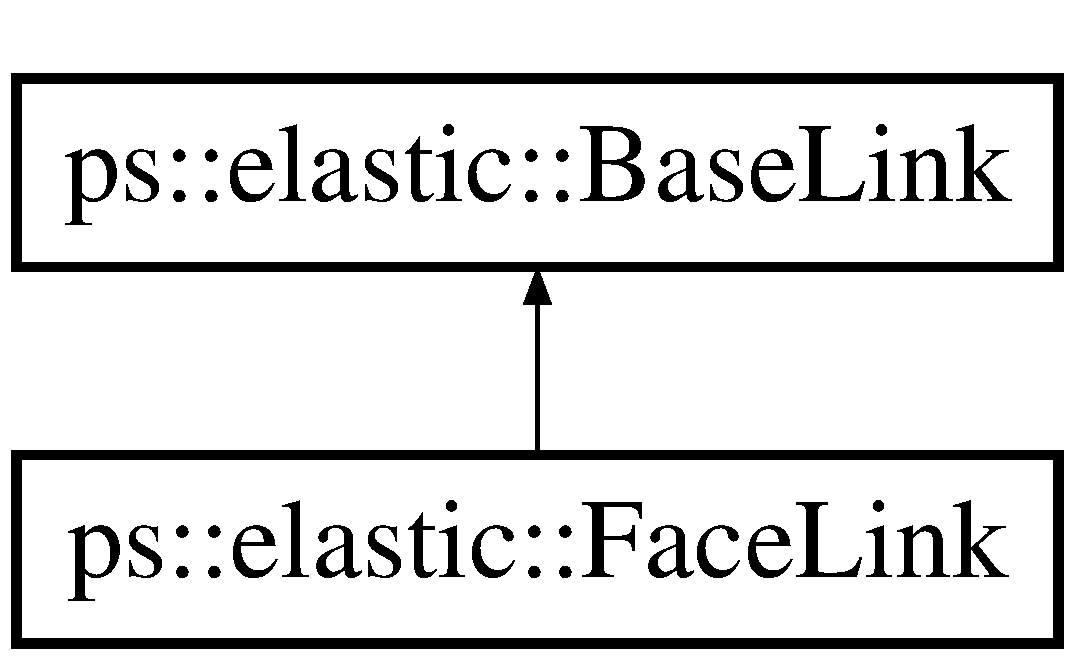
\includegraphics[height=2.000000cm]{classps_1_1elastic_1_1FaceLink}
\end{center}
\end{figure}
\subsection*{Static Public Member Functions}
\begin{DoxyCompactItemize}
\item 
\hypertarget{classps_1_1elastic_1_1FaceLink_aa38f226864df8220d1e67cb74032dbdb}{}static \hyperlink{classps_1_1elastic_1_1FaceLink}{Face\+Link} {\bfseries create} (U32 idx)\label{classps_1_1elastic_1_1FaceLink_aa38f226864df8220d1e67cb74032dbdb}

\end{DoxyCompactItemize}
\subsection*{Additional Inherited Members}


The documentation for this class was generated from the following file\+:\begin{DoxyCompactItemize}
\item 
/\+Users/pourya/\+Desktop/platform/repos/tetcutter/src/elastic/volmeshentities.\+h\end{DoxyCompactItemize}

\hypertarget{classps_1_1FastAccessNamedResource}{}\section{ps\+:\+:Fast\+Access\+Named\+Resource$<$ T, Policy\+Resource\+Type, Policy\+Resource\+Insert\+Remove, Policy\+Error\+Logging, allow\+Duplicates $>$ Class Template Reference}
\label{classps_1_1FastAccessNamedResource}\index{ps\+::\+Fast\+Access\+Named\+Resource$<$ T, Policy\+Resource\+Type, Policy\+Resource\+Insert\+Remove, Policy\+Error\+Logging, allow\+Duplicates $>$@{ps\+::\+Fast\+Access\+Named\+Resource$<$ T, Policy\+Resource\+Type, Policy\+Resource\+Insert\+Remove, Policy\+Error\+Logging, allow\+Duplicates $>$}}
Inheritance diagram for ps\+:\+:Fast\+Access\+Named\+Resource$<$ T, Policy\+Resource\+Type, Policy\+Resource\+Insert\+Remove, Policy\+Error\+Logging, allow\+Duplicates $>$\+:\begin{figure}[H]
\begin{center}
\leavevmode
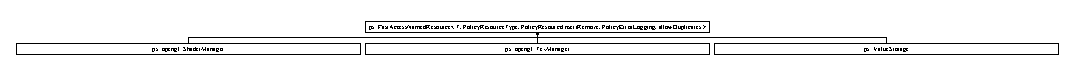
\includegraphics[height=0.501119cm]{classps_1_1FastAccessNamedResource}
\end{center}
\end{figure}
\subsection*{Public Types}
\begin{DoxyCompactItemize}
\item 
\hypertarget{classps_1_1FastAccessNamedResource_a6af3539e0c649fd152cb382331d49c05}{}typedef Policy\+Resource\+Type$<$ T $>$\+::Resource {\bfseries Resource}\label{classps_1_1FastAccessNamedResource_a6af3539e0c649fd152cb382331d49c05}

\item 
\hypertarget{classps_1_1FastAccessNamedResource_aac61fb6378f6c21cc01f315677339498}{}typedef std\+::unordered\+\_\+map$<$ string, Resource $>$\+::iterator {\bfseries I\+T\+E\+R}\label{classps_1_1FastAccessNamedResource_aac61fb6378f6c21cc01f315677339498}

\item 
\hypertarget{classps_1_1FastAccessNamedResource_a01908e03a2c91705ca74bb5ef6a955cb}{}typedef std\+::unordered\+\_\+map$<$ string, Resource $>$\+::const\+\_\+iterator {\bfseries C\+O\+N\+S\+T\+\_\+\+I\+T\+E\+R}\label{classps_1_1FastAccessNamedResource_a01908e03a2c91705ca74bb5ef6a955cb}

\end{DoxyCompactItemize}
\subsection*{Public Member Functions}
\begin{DoxyCompactItemize}
\item 
bool \hyperlink{classps_1_1FastAccessNamedResource_ac781dbc4f970d458bf8bfc5ef9896df6}{has} (const char $\ast$name) const 
\begin{DoxyCompactList}\small\item\em has checks weather a named resource is present in the collection \end{DoxyCompactList}\item 
Resource \hyperlink{classps_1_1FastAccessNamedResource_a10068de137ce1cada217b3e99992a431}{get} (const char $\ast$name) const 
\begin{DoxyCompactList}\small\item\em get \end{DoxyCompactList}\item 
\hypertarget{classps_1_1FastAccessNamedResource_a25f0d1aab3afa15fce7fe59d8c732b97}{}I\+T\+E\+R {\bfseries at} (const char $\ast$name)\label{classps_1_1FastAccessNamedResource_a25f0d1aab3afa15fce7fe59d8c732b97}

\item 
\hypertarget{classps_1_1FastAccessNamedResource_aba96d2a7d5ce1b8c1d6249712066c095}{}bool {\bfseries set} (const char $\ast$name, const Resource \&element)\label{classps_1_1FastAccessNamedResource_aba96d2a7d5ce1b8c1d6249712066c095}

\item 
bool \hyperlink{classps_1_1FastAccessNamedResource_a768ce90516cc7ed73f4f439cbccbc4ea}{add} (const Resource \&element, const char $\ast$name)
\begin{DoxyCompactList}\small\item\em add will add an element into the hashmap \end{DoxyCompactList}\item 
\hypertarget{classps_1_1FastAccessNamedResource_a3f5f275abd2f7ef8e90d4bd84965239c}{}bool {\bfseries remove} (const char $\ast$name)\label{classps_1_1FastAccessNamedResource_a3f5f275abd2f7ef8e90d4bd84965239c}

\item 
\hypertarget{classps_1_1FastAccessNamedResource_a0998b26ab4c2d1a25cc18c6791fc0c82}{}void {\bfseries cleanup} ()\label{classps_1_1FastAccessNamedResource_a0998b26ab4c2d1a25cc18c6791fc0c82}

\item 
\hypertarget{classps_1_1FastAccessNamedResource_a4053b80e5555ecdab7970404e564c3c6}{}U32 {\bfseries size} () const \label{classps_1_1FastAccessNamedResource_a4053b80e5555ecdab7970404e564c3c6}

\item 
\hypertarget{classps_1_1FastAccessNamedResource_afed3ed3697e3af465bf7f87e6ff6f430}{}C\+O\+N\+S\+T\+\_\+\+I\+T\+E\+R {\bfseries cbegin} () const \label{classps_1_1FastAccessNamedResource_afed3ed3697e3af465bf7f87e6ff6f430}

\item 
\hypertarget{classps_1_1FastAccessNamedResource_add5d7e074b8c71e8f203c58d28029bb2}{}C\+O\+N\+S\+T\+\_\+\+I\+T\+E\+R {\bfseries cend} () const \label{classps_1_1FastAccessNamedResource_add5d7e074b8c71e8f203c58d28029bb2}

\item 
\hypertarget{classps_1_1FastAccessNamedResource_ac7eadf05030c0db15c98a4a5bebf066f}{}I\+T\+E\+R {\bfseries begin} ()\label{classps_1_1FastAccessNamedResource_ac7eadf05030c0db15c98a4a5bebf066f}

\item 
\hypertarget{classps_1_1FastAccessNamedResource_a970641642502283ce3de57eb11edb06d}{}I\+T\+E\+R {\bfseries end} ()\label{classps_1_1FastAccessNamedResource_a970641642502283ce3de57eb11edb06d}

\item 
\hypertarget{classps_1_1FastAccessNamedResource_a84a30a22f21d084019dc3f0622ab81b7}{}Resource {\bfseries operator\mbox{[}$\,$\mbox{]}} (const char $\ast$name)\label{classps_1_1FastAccessNamedResource_a84a30a22f21d084019dc3f0622ab81b7}

\end{DoxyCompactItemize}
\subsection*{Protected Attributes}
\begin{DoxyCompactItemize}
\item 
\hypertarget{classps_1_1FastAccessNamedResource_a1aa9cbd37a93fe951c6fefa8e094dea6}{}std\+::unordered\+\_\+map$<$ string, Resource $>$ {\bfseries m\+\_\+hash}\label{classps_1_1FastAccessNamedResource_a1aa9cbd37a93fe951c6fefa8e094dea6}

\end{DoxyCompactItemize}


\subsection{Member Function Documentation}
\hypertarget{classps_1_1FastAccessNamedResource_a768ce90516cc7ed73f4f439cbccbc4ea}{}\index{ps\+::\+Fast\+Access\+Named\+Resource@{ps\+::\+Fast\+Access\+Named\+Resource}!add@{add}}
\index{add@{add}!ps\+::\+Fast\+Access\+Named\+Resource@{ps\+::\+Fast\+Access\+Named\+Resource}}
\subsubsection[{add(const Resource \&element, const char $\ast$name)}]{\setlength{\rightskip}{0pt plus 5cm}template$<$typename T, template$<$ class $>$ class Policy\+Resource\+Type = Type\+Pointer, template$<$ class $>$ class Policy\+Resource\+Insert\+Remove = Noop\+Insert\+Remove\+By\+Safe\+Delete, class Policy\+Error\+Logging = Logging, bool allow\+Duplicates = false$>$ bool {\bf ps\+::\+Fast\+Access\+Named\+Resource}$<$ T, Policy\+Resource\+Type, Policy\+Resource\+Insert\+Remove, Policy\+Error\+Logging, allow\+Duplicates $>$\+::add (
\begin{DoxyParamCaption}
\item[{const Resource \&}]{element, }
\item[{const char $\ast$}]{name}
\end{DoxyParamCaption}
)\hspace{0.3cm}{\ttfamily [inline]}}\label{classps_1_1FastAccessNamedResource_a768ce90516cc7ed73f4f439cbccbc4ea}


add will add an element into the hashmap 


\begin{DoxyParams}{Parameters}
{\em element} & \\
\hline
{\em name} & \\
\hline
\end{DoxyParams}
\hypertarget{classps_1_1FastAccessNamedResource_a10068de137ce1cada217b3e99992a431}{}\index{ps\+::\+Fast\+Access\+Named\+Resource@{ps\+::\+Fast\+Access\+Named\+Resource}!get@{get}}
\index{get@{get}!ps\+::\+Fast\+Access\+Named\+Resource@{ps\+::\+Fast\+Access\+Named\+Resource}}
\subsubsection[{get(const char $\ast$name) const }]{\setlength{\rightskip}{0pt plus 5cm}template$<$typename T, template$<$ class $>$ class Policy\+Resource\+Type = Type\+Pointer, template$<$ class $>$ class Policy\+Resource\+Insert\+Remove = Noop\+Insert\+Remove\+By\+Safe\+Delete, class Policy\+Error\+Logging = Logging, bool allow\+Duplicates = false$>$ Resource {\bf ps\+::\+Fast\+Access\+Named\+Resource}$<$ T, Policy\+Resource\+Type, Policy\+Resource\+Insert\+Remove, Policy\+Error\+Logging, allow\+Duplicates $>$\+::get (
\begin{DoxyParamCaption}
\item[{const char $\ast$}]{name}
\end{DoxyParamCaption}
) const\hspace{0.3cm}{\ttfamily [inline]}}\label{classps_1_1FastAccessNamedResource_a10068de137ce1cada217b3e99992a431}


get 


\begin{DoxyParams}{Parameters}
{\em name} & \\
\hline
\end{DoxyParams}
\begin{DoxyReturn}{Returns}

\end{DoxyReturn}
\hypertarget{classps_1_1FastAccessNamedResource_ac781dbc4f970d458bf8bfc5ef9896df6}{}\index{ps\+::\+Fast\+Access\+Named\+Resource@{ps\+::\+Fast\+Access\+Named\+Resource}!has@{has}}
\index{has@{has}!ps\+::\+Fast\+Access\+Named\+Resource@{ps\+::\+Fast\+Access\+Named\+Resource}}
\subsubsection[{has(const char $\ast$name) const }]{\setlength{\rightskip}{0pt plus 5cm}template$<$typename T, template$<$ class $>$ class Policy\+Resource\+Type = Type\+Pointer, template$<$ class $>$ class Policy\+Resource\+Insert\+Remove = Noop\+Insert\+Remove\+By\+Safe\+Delete, class Policy\+Error\+Logging = Logging, bool allow\+Duplicates = false$>$ bool {\bf ps\+::\+Fast\+Access\+Named\+Resource}$<$ T, Policy\+Resource\+Type, Policy\+Resource\+Insert\+Remove, Policy\+Error\+Logging, allow\+Duplicates $>$\+::has (
\begin{DoxyParamCaption}
\item[{const char $\ast$}]{name}
\end{DoxyParamCaption}
) const\hspace{0.3cm}{\ttfamily [inline]}}\label{classps_1_1FastAccessNamedResource_ac781dbc4f970d458bf8bfc5ef9896df6}


has checks weather a named resource is present in the collection 


\begin{DoxyParams}{Parameters}
{\em name} & the title of the resource \\
\hline
\end{DoxyParams}
\begin{DoxyReturn}{Returns}
true if the item is found in the collection 
\end{DoxyReturn}


The documentation for this class was generated from the following file\+:\begin{DoxyCompactItemize}
\item 
/\+Users/pourya/\+Desktop/platform/repos/tetcutter/src/base/resourcemanager.\+h\end{DoxyCompactItemize}

\hypertarget{classps_1_1scene_1_1Geometry}{}\section{ps\+:\+:scene\+:\+:Geometry Class Reference}
\label{classps_1_1scene_1_1Geometry}\index{ps\+::scene\+::\+Geometry@{ps\+::scene\+::\+Geometry}}
\subsection*{Public Member Functions}
\begin{DoxyCompactItemize}
\item 
\hypertarget{classps_1_1scene_1_1Geometry_a2d4f58b106041e3a758086577366aa9e}{}{\bfseries Geometry} (const \hyperlink{classps_1_1scene_1_1Geometry}{Geometry} \&other)\label{classps_1_1scene_1_1Geometry_a2d4f58b106041e3a758086577366aa9e}

\item 
\hypertarget{classps_1_1scene_1_1Geometry_af119f2be0cff8974051dfca0371b11bc}{}{\bfseries Geometry} (const \hyperlink{classps_1_1base_1_1CAString}{Ansi\+Str} \&str\+File\+Path)\label{classps_1_1scene_1_1Geometry_af119f2be0cff8974051dfca0371b11bc}

\item 
\hypertarget{classps_1_1scene_1_1Geometry_a82f44380754747b70333fa1f8bb6f320}{}void {\bfseries init} ()\label{classps_1_1scene_1_1Geometry_a82f44380754747b70333fa1f8bb6f320}

\item 
\hypertarget{classps_1_1scene_1_1Geometry_a9bfe3529ee6f25c12fbf87606b03ebab}{}void {\bfseries init} (int step\+Vertex, int step\+Color, int step\+Tex\+Coords, ps\+::opengl\+::\+G\+L\+Face\+Type face\+Mode=ft\+Triangles)\label{classps_1_1scene_1_1Geometry_a9bfe3529ee6f25c12fbf87606b03ebab}

\item 
\hypertarget{classps_1_1scene_1_1Geometry_a47cb57a90830d8e1982430174442c641}{}bool {\bfseries is\+Compatible} (const \hyperlink{classps_1_1scene_1_1Geometry}{Geometry} \&other) const \label{classps_1_1scene_1_1Geometry_a47cb57a90830d8e1982430174442c641}

\item 
\hypertarget{classps_1_1scene_1_1Geometry_a649e3aa04db6c185fed04c29d4e9a0ca}{}int {\bfseries count\+Vertices} () const \label{classps_1_1scene_1_1Geometry_a649e3aa04db6c185fed04c29d4e9a0ca}

\item 
\hypertarget{classps_1_1scene_1_1Geometry_a7f2f57051355459e6058794e99791336}{}int {\bfseries count\+Color} () const \label{classps_1_1scene_1_1Geometry_a7f2f57051355459e6058794e99791336}

\item 
\hypertarget{classps_1_1scene_1_1Geometry_adaf21771528e432d7d49501d0cb6e562}{}int {\bfseries count\+Tex\+Coords} () const \label{classps_1_1scene_1_1Geometry_adaf21771528e432d7d49501d0cb6e562}

\item 
\hypertarget{classps_1_1scene_1_1Geometry_a3ff0a8b4a7413a0d090032e8b0ee60b4}{}int {\bfseries count\+Normals} () const \label{classps_1_1scene_1_1Geometry_a3ff0a8b4a7413a0d090032e8b0ee60b4}

\item 
\hypertarget{classps_1_1scene_1_1Geometry_a21f6c67afbdc6d325d6158e3e593c3a1}{}int {\bfseries count\+Faces} () const \label{classps_1_1scene_1_1Geometry_a21f6c67afbdc6d325d6158e3e593c3a1}

\item 
\hypertarget{classps_1_1scene_1_1Geometry_a0b31979b990126792a93e61205f2f2c4}{}int {\bfseries get\+Vertex\+Step} () const \label{classps_1_1scene_1_1Geometry_a0b31979b990126792a93e61205f2f2c4}

\item 
\hypertarget{classps_1_1scene_1_1Geometry_a6e4b43ed9010359f119faa807a278731}{}int {\bfseries get\+Color\+Step} () const \label{classps_1_1scene_1_1Geometry_a6e4b43ed9010359f119faa807a278731}

\item 
\hypertarget{classps_1_1scene_1_1Geometry_a296f6df4ff99976c6a5222f18977a7b4}{}int {\bfseries get\+Tex\+Coord\+Step} () const \label{classps_1_1scene_1_1Geometry_a296f6df4ff99976c6a5222f18977a7b4}

\item 
\hypertarget{classps_1_1scene_1_1Geometry_add26b3367413eb76182715262437cfce}{}int {\bfseries get\+Face\+Step} () const \label{classps_1_1scene_1_1Geometry_add26b3367413eb76182715262437cfce}

\item 
\hypertarget{classps_1_1scene_1_1Geometry_a5090a568778348417dca5fe5e8459bb2}{}G\+L\+Face\+Type {\bfseries get\+Face\+Mode} () const \label{classps_1_1scene_1_1Geometry_a5090a568778348417dca5fe5e8459bb2}

\item 
\hypertarget{classps_1_1scene_1_1Geometry_a06ecdb03a5103deba6dadf178e13203a}{}\hyperlink{classps_1_1base_1_1Vec3}{vec3f} {\bfseries vertex\+At} (int index) const \label{classps_1_1scene_1_1Geometry_a06ecdb03a5103deba6dadf178e13203a}

\item 
\hypertarget{classps_1_1scene_1_1Geometry_ad8c85379124d147cebd3ce69615535ed}{}\hyperlink{classps_1_1base_1_1Vec4}{vec4f} {\bfseries color\+At} (int index) const \label{classps_1_1scene_1_1Geometry_ad8c85379124d147cebd3ce69615535ed}

\item 
\hypertarget{classps_1_1scene_1_1Geometry_ad119e6a4850a56e93a2cd7c360a8be6d}{}\hyperlink{classps_1_1base_1_1Vec2}{vec2f} {\bfseries texcoord\+At} (int index) const \label{classps_1_1scene_1_1Geometry_ad119e6a4850a56e93a2cd7c360a8be6d}

\item 
\hypertarget{classps_1_1scene_1_1Geometry_a555d8d4442de50a13306307156986de7}{}\hyperlink{classps_1_1base_1_1Vec3}{vec3f} {\bfseries normal\+At} (int index) const \label{classps_1_1scene_1_1Geometry_a555d8d4442de50a13306307156986de7}

\item 
\hypertarget{classps_1_1scene_1_1Geometry_a4e4991f3059757475f26481dd205ea75}{}\hyperlink{classps_1_1base_1_1Vec3}{vec3u32} {\bfseries triangle\+At} (int index) const \label{classps_1_1scene_1_1Geometry_a4e4991f3059757475f26481dd205ea75}

\item 
\hypertarget{classps_1_1scene_1_1Geometry_aee4a0196a95f8372fa693954aba9a959}{}\hyperlink{classps_1_1base_1_1Vec4}{vec4u32} {\bfseries quad\+At} (int index) const \label{classps_1_1scene_1_1Geometry_aee4a0196a95f8372fa693954aba9a959}

\item 
\hypertarget{classps_1_1scene_1_1Geometry_a83cea61981c2767004582263dc808288}{}void {\bfseries set\+Vertex} (int index, const \hyperlink{classps_1_1base_1_1Vec3}{vec3f} \&v)\label{classps_1_1scene_1_1Geometry_a83cea61981c2767004582263dc808288}

\item 
\hypertarget{classps_1_1scene_1_1Geometry_a7be917968faf6256ddf2f9b1f7206c51}{}const vector$<$ float $>$ \& {\bfseries vertices} () const \label{classps_1_1scene_1_1Geometry_a7be917968faf6256ddf2f9b1f7206c51}

\item 
\hypertarget{classps_1_1scene_1_1Geometry_a7e12d02f26ea2ac9fe8d710a0ef50382}{}const vector$<$ float $>$ \& {\bfseries colors} () const \label{classps_1_1scene_1_1Geometry_a7e12d02f26ea2ac9fe8d710a0ef50382}

\item 
\hypertarget{classps_1_1scene_1_1Geometry_aac26873703c9b6239763edd0db900c48}{}const vector$<$ float $>$ \& {\bfseries texcoords} () const \label{classps_1_1scene_1_1Geometry_aac26873703c9b6239763edd0db900c48}

\item 
\hypertarget{classps_1_1scene_1_1Geometry_a69a5afa92fe0dc9089479238feb9e005}{}const vector$<$ float $>$ \& {\bfseries normals} () const \label{classps_1_1scene_1_1Geometry_a69a5afa92fe0dc9089479238feb9e005}

\item 
\hypertarget{classps_1_1scene_1_1Geometry_aaa74d9df99e92547553b65f73f6650cc}{}const vector$<$ U32 $>$ \& {\bfseries indices} () const \label{classps_1_1scene_1_1Geometry_aaa74d9df99e92547553b65f73f6650cc}

\item 
\hypertarget{classps_1_1scene_1_1Geometry_ac189febdbd60df86a1f2270d920cb6ad}{}vector$<$ float $>$ \& {\bfseries vertices} ()\label{classps_1_1scene_1_1Geometry_ac189febdbd60df86a1f2270d920cb6ad}

\item 
\hypertarget{classps_1_1scene_1_1Geometry_adedd00b50942ed1f4033be80a1e2587f}{}vector$<$ float $>$ \& {\bfseries colors} ()\label{classps_1_1scene_1_1Geometry_adedd00b50942ed1f4033be80a1e2587f}

\item 
\hypertarget{classps_1_1scene_1_1Geometry_a53d77248569cc8dd01dd6389315d2dd9}{}vector$<$ float $>$ \& {\bfseries texcoords} ()\label{classps_1_1scene_1_1Geometry_a53d77248569cc8dd01dd6389315d2dd9}

\item 
\hypertarget{classps_1_1scene_1_1Geometry_a806ba6c18509dbe3c07ed6cd585ebed5}{}vector$<$ float $>$ \& {\bfseries normals} ()\label{classps_1_1scene_1_1Geometry_a806ba6c18509dbe3c07ed6cd585ebed5}

\item 
\hypertarget{classps_1_1scene_1_1Geometry_acb3c84aaf54910396d59f0d3a6ebf51c}{}vector$<$ U32 $>$ \& {\bfseries indices} ()\label{classps_1_1scene_1_1Geometry_acb3c84aaf54910396d59f0d3a6ebf51c}

\item 
\hypertarget{classps_1_1scene_1_1Geometry_a1b0f3d342512b7b98946392ad010034f}{}bool {\bfseries add\+Vertex} (const \hyperlink{classps_1_1base_1_1Vec3}{vec3f} \&v)\label{classps_1_1scene_1_1Geometry_a1b0f3d342512b7b98946392ad010034f}

\item 
\hypertarget{classps_1_1scene_1_1Geometry_a4077b2edc4b78af20ed5cf4316e513e6}{}bool {\bfseries add\+Color} (const \hyperlink{classps_1_1base_1_1Vec4}{vec4f} \&c)\label{classps_1_1scene_1_1Geometry_a4077b2edc4b78af20ed5cf4316e513e6}

\item 
\hypertarget{classps_1_1scene_1_1Geometry_a8272fa2d8c2ef87de8624272da019ca5}{}bool {\bfseries add\+Tex\+Coord} (float t)\label{classps_1_1scene_1_1Geometry_a8272fa2d8c2ef87de8624272da019ca5}

\item 
\hypertarget{classps_1_1scene_1_1Geometry_a64ec7b280cd43ebecd94a9282e9ec875}{}bool {\bfseries add\+Tex\+Coord} (const \hyperlink{classps_1_1base_1_1Vec2}{vec2f} \&t)\label{classps_1_1scene_1_1Geometry_a64ec7b280cd43ebecd94a9282e9ec875}

\item 
\hypertarget{classps_1_1scene_1_1Geometry_a3573bc0a577cfde0d0af21e2ed2a3de1}{}bool {\bfseries add\+Tex\+Coord} (const \hyperlink{classps_1_1base_1_1Vec3}{vec3f} \&t)\label{classps_1_1scene_1_1Geometry_a3573bc0a577cfde0d0af21e2ed2a3de1}

\item 
\hypertarget{classps_1_1scene_1_1Geometry_a247bd8f84d43b77bf180ba093991ee3d}{}void {\bfseries add\+Normal} (const \hyperlink{classps_1_1base_1_1Vec3}{vec3f} \&n)\label{classps_1_1scene_1_1Geometry_a247bd8f84d43b77bf180ba093991ee3d}

\item 
\hypertarget{classps_1_1scene_1_1Geometry_a537a223546ac2ef6839453c1a143d49f}{}bool {\bfseries add\+Triangle} (const \hyperlink{classps_1_1base_1_1Vec3}{vec3u32} \&f)\label{classps_1_1scene_1_1Geometry_a537a223546ac2ef6839453c1a143d49f}

\item 
\hypertarget{classps_1_1scene_1_1Geometry_ac1e4ff204129c151ef34c17ea81d320e}{}bool {\bfseries add\+Quad} (const \hyperlink{classps_1_1base_1_1Vec4}{vec4u32} \&f)\label{classps_1_1scene_1_1Geometry_ac1e4ff204129c151ef34c17ea81d320e}

\item 
\hypertarget{classps_1_1scene_1_1Geometry_a5b2efd93099a82f875a2397e72efb1ba}{}void {\bfseries extrude} (const \hyperlink{classps_1_1base_1_1Vec3}{vec3f} \&v)\label{classps_1_1scene_1_1Geometry_a5b2efd93099a82f875a2397e72efb1ba}

\item 
\hypertarget{classps_1_1scene_1_1Geometry_ac1440ef0e4aec89e9a106803a8d2c8ce}{}void {\bfseries transform} (const \hyperlink{classps_1_1base_1_1Matrix}{mat44f} \&m)\label{classps_1_1scene_1_1Geometry_ac1440ef0e4aec89e9a106803a8d2c8ce}

\item 
\hypertarget{classps_1_1scene_1_1Geometry_a4a5837a775c3c462968aa1246b1d3dd4}{}bool {\bfseries add\+Vertex\+Attribs} (const vector$<$ float $>$ \&arr\+Attribs, int step=3, G\+L\+Buffer\+Type attrib\+Kind=gbt\+Position)\label{classps_1_1scene_1_1Geometry_a4a5837a775c3c462968aa1246b1d3dd4}

\item 
\hypertarget{classps_1_1scene_1_1Geometry_a971e48f7d21975c9d9fb3bb33eebff61}{}void {\bfseries add\+Per\+Vertex\+Color} (const \hyperlink{classps_1_1base_1_1Vec4}{vec4f} \&color, U32 ct\+Vertices=0)\label{classps_1_1scene_1_1Geometry_a971e48f7d21975c9d9fb3bb33eebff61}

\item 
\hypertarget{classps_1_1scene_1_1Geometry_a9446984e251746380d5d937b3f9c8c66}{}bool {\bfseries add\+Face\+Indices} (const vector$<$ U32 $>$ \&arr\+Index, ps\+::opengl\+::\+G\+L\+Face\+Type face\+Mode=ft\+Triangles)\label{classps_1_1scene_1_1Geometry_a9446984e251746380d5d937b3f9c8c66}

\item 
\hypertarget{classps_1_1scene_1_1Geometry_a2da64558da7dc7c30105a412d89844a9}{}bool {\bfseries compute\+Normals\+From\+Faces} ()\label{classps_1_1scene_1_1Geometry_a2da64558da7dc7c30105a412d89844a9}

\item 
\hypertarget{classps_1_1scene_1_1Geometry_ab38a57abecb8385ce93457a2b8747ea1}{}void {\bfseries clear\+Buffer} (G\+L\+Buffer\+Type btype)\label{classps_1_1scene_1_1Geometry_ab38a57abecb8385ce93457a2b8747ea1}

\item 
\hypertarget{classps_1_1scene_1_1Geometry_ae42cbd9fb650f1117c8c6a9ceb2e9132}{}bool {\bfseries add\+Line} (const \hyperlink{classps_1_1base_1_1Vec3}{vec3f} \&start, const \hyperlink{classps_1_1base_1_1Vec3}{vec3f} \&end)\label{classps_1_1scene_1_1Geometry_ae42cbd9fb650f1117c8c6a9ceb2e9132}

\item 
\hypertarget{classps_1_1scene_1_1Geometry_a1f5252fb223fa253fddb1f5b242ba198}{}bool {\bfseries add\+Lines} (const vector$<$ \hyperlink{classps_1_1base_1_1Vec3}{vec3f} $>$ \&vertices)\label{classps_1_1scene_1_1Geometry_a1f5252fb223fa253fddb1f5b242ba198}

\item 
\hypertarget{classps_1_1scene_1_1Geometry_a41c90f08b712b9109047283f702618d7}{}bool {\bfseries add\+Circle2\+D} (int sectors, float radius=1.\+0f, const vec3f \&o=vec3f(0, 0, 0))\label{classps_1_1scene_1_1Geometry_a41c90f08b712b9109047283f702618d7}

\item 
\hypertarget{classps_1_1scene_1_1Geometry_a0a0a565babb0dc53cd93e6190b8cc5d1}{}bool {\bfseries add\+Circle3\+D} (int sectors, float radius=1.\+0f, const vec3f \&o=vec3f(0, 0, 0))\label{classps_1_1scene_1_1Geometry_a0a0a565babb0dc53cd93e6190b8cc5d1}

\item 
\hypertarget{classps_1_1scene_1_1Geometry_ad13940852a3241a186c3bdaaa230d0f7}{}bool {\bfseries add\+Cone} (int sectors, float radius=1.\+0f, float width=1.\+0f, const vec3f \&o=vec3f(0, 0, 0))\label{classps_1_1scene_1_1Geometry_ad13940852a3241a186c3bdaaa230d0f7}

\item 
\hypertarget{classps_1_1scene_1_1Geometry_a76be3b4e69cc804537919b0c1fde78b7}{}void {\bfseries add\+Cube} (const \hyperlink{classps_1_1base_1_1Vec3}{vec3f} \&lower, const \hyperlink{classps_1_1base_1_1Vec3}{vec3f} \&upper)\label{classps_1_1scene_1_1Geometry_a76be3b4e69cc804537919b0c1fde78b7}

\item 
\hypertarget{classps_1_1scene_1_1Geometry_ae91b7f0e9dbacf75a155dd22243d5475}{}void {\bfseries add\+Cube} (const \hyperlink{classps_1_1base_1_1Vec3}{vec3f} \&center, float side)\label{classps_1_1scene_1_1Geometry_ae91b7f0e9dbacf75a155dd22243d5475}

\item 
\hypertarget{classps_1_1scene_1_1Geometry_ab75767952a0dca9d0161882ebd642d75}{}void {\bfseries add\+Sphere} (float radius=1.\+0f, int hseg=8, int vseg=8)\label{classps_1_1scene_1_1Geometry_ab75767952a0dca9d0161882ebd642d75}

\item 
\hypertarget{classps_1_1scene_1_1Geometry_a68187bda9650b5f12a50404300dbc85a}{}void {\bfseries add\+Cylinder} (float radius, float height, int sectors, bool base=true, bool roof=true)\label{classps_1_1scene_1_1Geometry_a68187bda9650b5f12a50404300dbc85a}

\item 
\hypertarget{classps_1_1scene_1_1Geometry_a18786c70964eb9533aabea2ce2002db9}{}void {\bfseries add\+Tetrahedra} (\hyperlink{classps_1_1base_1_1Vec3}{vec3f} v\mbox{[}4\mbox{]})\label{classps_1_1scene_1_1Geometry_a18786c70964eb9533aabea2ce2002db9}

\item 
\hypertarget{classps_1_1scene_1_1Geometry_af5ca854d61987b909706795e80c6d354}{}void {\bfseries add\+Tetrahedra} (const vector$<$ float $>$ \&vertices, const vector$<$ U32 $>$ \&tets)\label{classps_1_1scene_1_1Geometry_af5ca854d61987b909706795e80c6d354}

\item 
bool \hyperlink{classps_1_1scene_1_1Geometry_ac43ea1de489b810baf386094f1900324}{add\+Ring\+Strip\+Around\+X\+Axis} (int sectors, float radius, float thickness, const \hyperlink{classps_1_1base_1_1Vec3}{vec3f} \&origin)
\item 
bool \hyperlink{classps_1_1scene_1_1Geometry_af87d017d6d893342c956c9757100b4b4}{add\+Disc} (int sectors, int xsections, float radius, float thickness, const \hyperlink{classps_1_1base_1_1Vec3}{vec3f} \&o=\hyperlink{classps_1_1base_1_1Vec3}{vec3f}(0, 0, 0))
\item 
\hypertarget{classps_1_1scene_1_1Geometry_a789daa85947087c0f18c3cc1bf3f9b44}{}bool {\bfseries check\+Indices} () const \label{classps_1_1scene_1_1Geometry_a789daa85947087c0f18c3cc1bf3f9b44}

\item 
\hypertarget{classps_1_1scene_1_1Geometry_a338342fe4822f8417b15ced15ee05aa0}{}\hyperlink{classps_1_1base_1_1AABB}{A\+A\+B\+B} {\bfseries aabb} () const \label{classps_1_1scene_1_1Geometry_a338342fe4822f8417b15ced15ee05aa0}

\item 
\hypertarget{classps_1_1scene_1_1Geometry_afd7fd6c6fa3fa5bad250c2a4e58a2567}{}bool {\bfseries copy\+From} (const \hyperlink{classps_1_1scene_1_1Geometry}{Geometry} \&other)\label{classps_1_1scene_1_1Geometry_afd7fd6c6fa3fa5bad250c2a4e58a2567}

\item 
\hypertarget{classps_1_1scene_1_1Geometry_a4d0267516367ea59f30e8b6ffdb34b46}{}bool {\bfseries append\+From} (const \hyperlink{classps_1_1scene_1_1Geometry}{Geometry} \&other)\label{classps_1_1scene_1_1Geometry_a4d0267516367ea59f30e8b6ffdb34b46}

\item 
\hypertarget{classps_1_1scene_1_1Geometry_a4a6d0254f3577b1d980969ae7a446898}{}bool {\bfseries read} (const \hyperlink{classps_1_1base_1_1CAString}{Ansi\+Str} \&str\+File\+Path)\label{classps_1_1scene_1_1Geometry_a4a6d0254f3577b1d980969ae7a446898}

\item 
\hypertarget{classps_1_1scene_1_1Geometry_af566f04872e05cc1d25538e42d12ab5c}{}bool {\bfseries write} (const \hyperlink{classps_1_1base_1_1CAString}{Ansi\+Str} \&str\+File\+Path) const \label{classps_1_1scene_1_1Geometry_af566f04872e05cc1d25538e42d12ab5c}

\item 
\hypertarget{classps_1_1scene_1_1Geometry_af3b2f797e03d1e270ef27c401af6a38f}{}bool {\bfseries read\+Obj} (const \hyperlink{classps_1_1base_1_1CAString}{Ansi\+Str} \&str\+File\+Path)\label{classps_1_1scene_1_1Geometry_af3b2f797e03d1e270ef27c401af6a38f}

\item 
\hypertarget{classps_1_1scene_1_1Geometry_aaa508ea83d9c52a13b9da5cfb552899e}{}bool {\bfseries write\+Obj} (const \hyperlink{classps_1_1base_1_1CAString}{Ansi\+Str} \&str\+File\+Path) const \label{classps_1_1scene_1_1Geometry_aaa508ea83d9c52a13b9da5cfb552899e}

\item 
\hypertarget{classps_1_1scene_1_1Geometry_aaa533b5ce841b233c687826e65ee9e72}{}\hyperlink{classps_1_1scene_1_1Geometry}{Geometry} \& {\bfseries operator=} (const \hyperlink{classps_1_1scene_1_1Geometry}{Geometry} \&other)\label{classps_1_1scene_1_1Geometry_aaa533b5ce841b233c687826e65ee9e72}

\item 
\hypertarget{classps_1_1scene_1_1Geometry_a40f16014af7b1c1dd4b9999c159cfcce}{}\hyperlink{classps_1_1scene_1_1Geometry}{Geometry} {\bfseries operator+} (const \hyperlink{classps_1_1scene_1_1Geometry}{Geometry} \&other) const \label{classps_1_1scene_1_1Geometry_a40f16014af7b1c1dd4b9999c159cfcce}

\end{DoxyCompactItemize}
\subsection*{Protected Member Functions}
\begin{DoxyCompactItemize}
\item 
\hypertarget{classps_1_1scene_1_1Geometry_a5c8446bd7ba7765e032d1e1033d07ff6}{}void {\bfseries cleanup} ()\label{classps_1_1scene_1_1Geometry_a5c8446bd7ba7765e032d1e1033d07ff6}

\end{DoxyCompactItemize}


\subsection{Member Function Documentation}
\hypertarget{classps_1_1scene_1_1Geometry_af87d017d6d893342c956c9757100b4b4}{}\index{ps\+::scene\+::\+Geometry@{ps\+::scene\+::\+Geometry}!add\+Disc@{add\+Disc}}
\index{add\+Disc@{add\+Disc}!ps\+::scene\+::\+Geometry@{ps\+::scene\+::\+Geometry}}
\subsubsection[{add\+Disc(int sectors, int xsections, float radius, float thickness, const vec3f \&o=vec3f(0, 0, 0))}]{\setlength{\rightskip}{0pt plus 5cm}bool Geometry\+::add\+Disc (
\begin{DoxyParamCaption}
\item[{int}]{sectors, }
\item[{int}]{xsections, }
\item[{float}]{radius, }
\item[{float}]{thickness, }
\item[{const {\bf vec3f} \&}]{o = {\ttfamily {\bf vec3f}(0,0,0)}}
\end{DoxyParamCaption}
)}\label{classps_1_1scene_1_1Geometry_af87d017d6d893342c956c9757100b4b4}
Add a disc to the geometry \hypertarget{classps_1_1scene_1_1Geometry_ac43ea1de489b810baf386094f1900324}{}\index{ps\+::scene\+::\+Geometry@{ps\+::scene\+::\+Geometry}!add\+Ring\+Strip\+Around\+X\+Axis@{add\+Ring\+Strip\+Around\+X\+Axis}}
\index{add\+Ring\+Strip\+Around\+X\+Axis@{add\+Ring\+Strip\+Around\+X\+Axis}!ps\+::scene\+::\+Geometry@{ps\+::scene\+::\+Geometry}}
\subsubsection[{add\+Ring\+Strip\+Around\+X\+Axis(int sectors, float radius, float thickness, const vec3f \&origin)}]{\setlength{\rightskip}{0pt plus 5cm}bool Geometry\+::add\+Ring\+Strip\+Around\+X\+Axis (
\begin{DoxyParamCaption}
\item[{int}]{sectors, }
\item[{float}]{radius, }
\item[{float}]{thickness, }
\item[{const {\bf vec3f} \&}]{origin}
\end{DoxyParamCaption}
)}\label{classps_1_1scene_1_1Geometry_ac43ea1de489b810baf386094f1900324}
Add a ring to the geometry 

The documentation for this class was generated from the following files\+:\begin{DoxyCompactItemize}
\item 
/\+Users/pourya/\+Desktop/platform/repos/tetcutter/src/scene/geometry.\+h\item 
/\+Users/pourya/\+Desktop/platform/repos/tetcutter/src/scene/geometry.\+cpp\end{DoxyCompactItemize}

\hypertarget{classps_1_1scene_1_1GizmoAvatar}{}\section{ps\+:\+:scene\+:\+:Gizmo\+Avatar Class Reference}
\label{classps_1_1scene_1_1GizmoAvatar}\index{ps\+::scene\+::\+Gizmo\+Avatar@{ps\+::scene\+::\+Gizmo\+Avatar}}
Inheritance diagram for ps\+:\+:scene\+:\+:Gizmo\+Avatar\+:\begin{figure}[H]
\begin{center}
\leavevmode
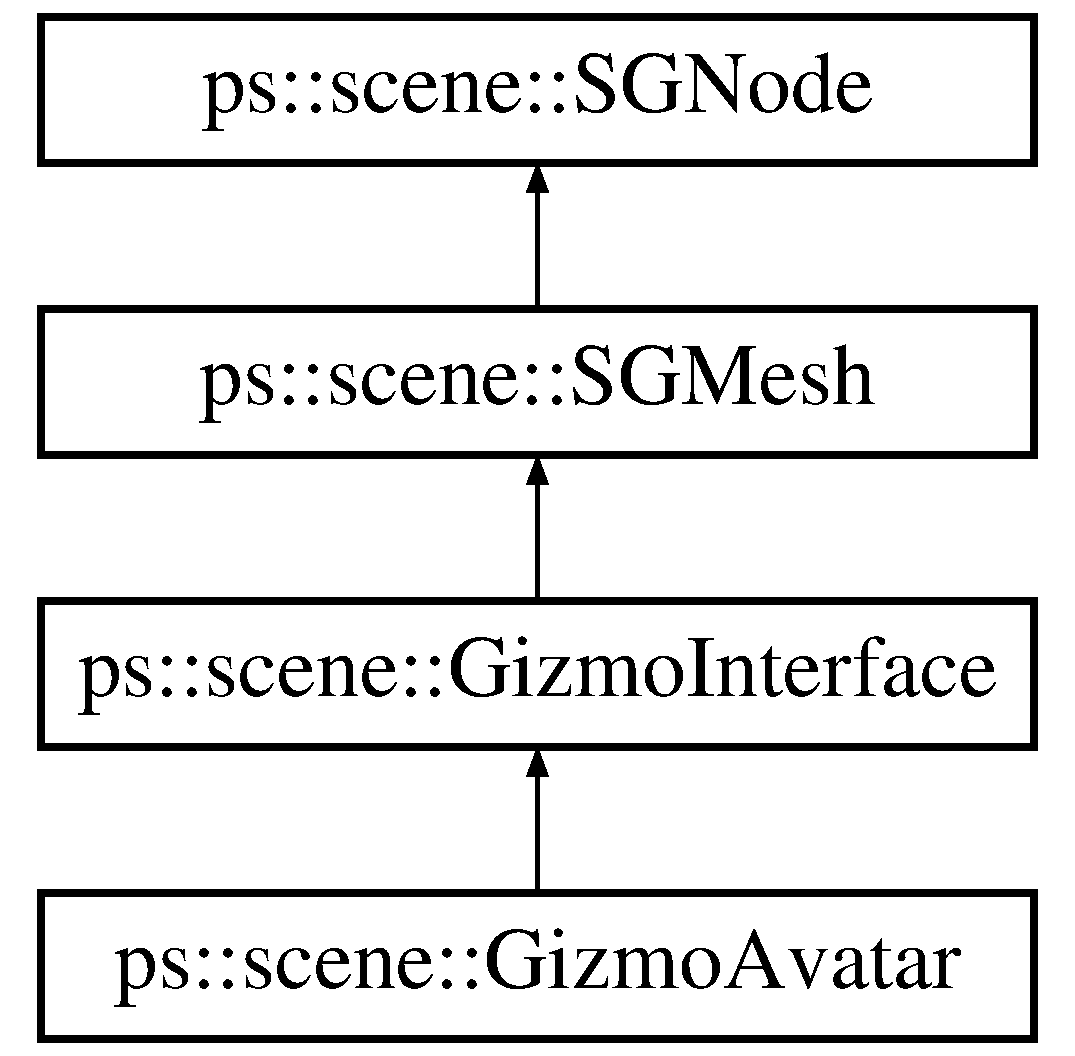
\includegraphics[height=4.000000cm]{classps_1_1scene_1_1GizmoAvatar}
\end{center}
\end{figure}
\subsection*{Protected Member Functions}
\begin{DoxyCompactItemize}
\item 
\hypertarget{classps_1_1scene_1_1GizmoAvatar_a0109b1363d93e3be2d32a9499e6458b8}{}void {\bfseries setup} ()\label{classps_1_1scene_1_1GizmoAvatar_a0109b1363d93e3be2d32a9499e6458b8}

\end{DoxyCompactItemize}
\subsection*{Additional Inherited Members}


The documentation for this class was generated from the following files\+:\begin{DoxyCompactItemize}
\item 
/\+Users/pourya/\+Desktop/platform/repos/tetcutter/src/scene/gizmo.\+h\item 
/\+Users/pourya/\+Desktop/platform/repos/tetcutter/src/scene/gizmo.\+cpp\end{DoxyCompactItemize}

\hypertarget{classps_1_1scene_1_1GizmoEffect}{}\section{ps\+:\+:scene\+:\+:Gizmo\+Effect Class Reference}
\label{classps_1_1scene_1_1GizmoEffect}\index{ps\+::scene\+::\+Gizmo\+Effect@{ps\+::scene\+::\+Gizmo\+Effect}}
Inheritance diagram for ps\+:\+:scene\+:\+:Gizmo\+Effect\+:\begin{figure}[H]
\begin{center}
\leavevmode
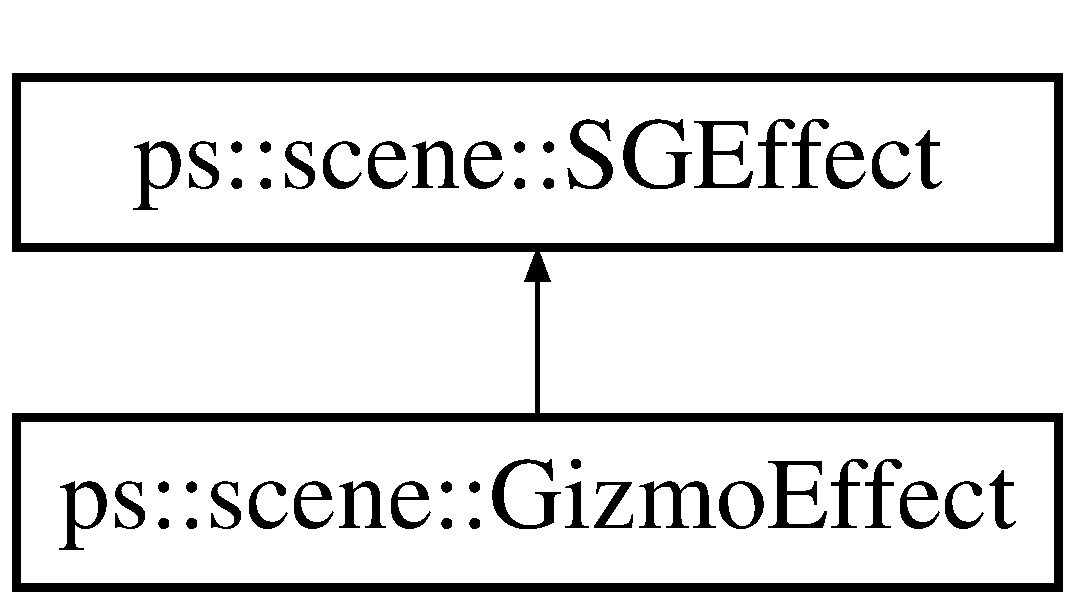
\includegraphics[height=2.000000cm]{classps_1_1scene_1_1GizmoEffect}
\end{center}
\end{figure}
\subsection*{Public Member Functions}
\begin{DoxyCompactItemize}
\item 
\hypertarget{classps_1_1scene_1_1GizmoEffect_a8b11c9fcc2117ad66d054ea3d3ecb469}{}{\bfseries Gizmo\+Effect} (\hyperlink{classps_1_1opengl_1_1GLShader}{G\+L\+Shader} $\ast$s)\label{classps_1_1scene_1_1GizmoEffect_a8b11c9fcc2117ad66d054ea3d3ecb469}

\item 
\hypertarget{classps_1_1scene_1_1GizmoEffect_a9afa3aa81d4f8077684a08aa945aa16d}{}void {\bfseries set\+Color} (const \hyperlink{classps_1_1base_1_1Vec4}{vec4f} \&color)\label{classps_1_1scene_1_1GizmoEffect_a9afa3aa81d4f8077684a08aa945aa16d}

\item 
\hypertarget{classps_1_1scene_1_1GizmoEffect_a8bcd44e759c32386b5835dc2fe5f927e}{}void {\bfseries bind} ()\label{classps_1_1scene_1_1GizmoEffect_a8bcd44e759c32386b5835dc2fe5f927e}

\end{DoxyCompactItemize}
\subsection*{Additional Inherited Members}


The documentation for this class was generated from the following file\+:\begin{DoxyCompactItemize}
\item 
/\+Users/pourya/\+Desktop/platform/repos/tetcutter/src/scene/gizmo.\+cpp\end{DoxyCompactItemize}

\hypertarget{classps_1_1scene_1_1GizmoInterface}{}\section{ps\+:\+:scene\+:\+:Gizmo\+Interface Class Reference}
\label{classps_1_1scene_1_1GizmoInterface}\index{ps\+::scene\+::\+Gizmo\+Interface@{ps\+::scene\+::\+Gizmo\+Interface}}
Inheritance diagram for ps\+:\+:scene\+:\+:Gizmo\+Interface\+:\begin{figure}[H]
\begin{center}
\leavevmode
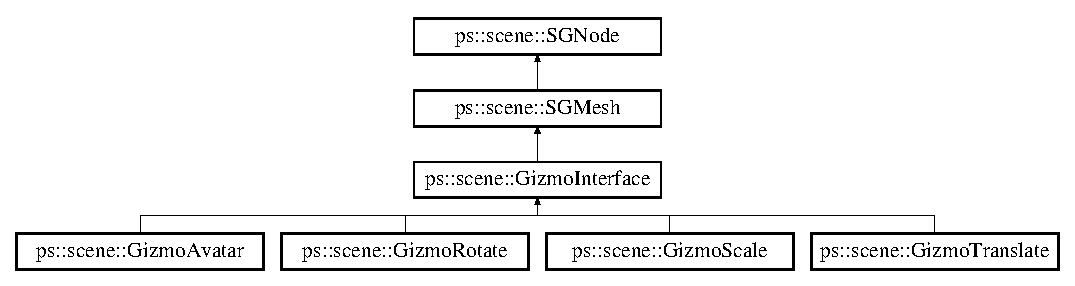
\includegraphics[height=3.393939cm]{classps_1_1scene_1_1GizmoInterface}
\end{center}
\end{figure}
\subsection*{Public Member Functions}
\begin{DoxyCompactItemize}
\item 
\hypertarget{classps_1_1scene_1_1GizmoInterface_a3d8d2479ac8edc86bc3cdfe3161cece1}{}Gizmo\+Axis {\bfseries axis} () const \label{classps_1_1scene_1_1GizmoInterface_a3d8d2479ac8edc86bc3cdfe3161cece1}

\item 
\hypertarget{classps_1_1scene_1_1GizmoInterface_af83f0e916e3037a3fac3acf1f925be54}{}void {\bfseries set\+Axis} (Gizmo\+Axis axis)\label{classps_1_1scene_1_1GizmoInterface_af83f0e916e3037a3fac3acf1f925be54}

\item 
\hypertarget{classps_1_1scene_1_1GizmoInterface_ac506854a9d644957bba1d44892e62454}{}virtual int {\bfseries set\+Axis} (const \hyperlink{classps_1_1base_1_1Ray}{Ray} \&r)\label{classps_1_1scene_1_1GizmoInterface_ac506854a9d644957bba1d44892e62454}

\item 
\hypertarget{classps_1_1scene_1_1GizmoInterface_a567abdf171320701708f2bfa97cac858}{}\hyperlink{classps_1_1base_1_1Vec4}{vec4f} {\bfseries axis\+Color} (Gizmo\+Axis a)\label{classps_1_1scene_1_1GizmoInterface_a567abdf171320701708f2bfa97cac858}

\end{DoxyCompactItemize}
\subsection*{Protected Attributes}
\begin{DoxyCompactItemize}
\item 
\hypertarget{classps_1_1scene_1_1GizmoInterface_a34badbe2f7a82833fcf6a0e6468c793c}{}Gizmo\+Axis {\bfseries m\+\_\+axis}\label{classps_1_1scene_1_1GizmoInterface_a34badbe2f7a82833fcf6a0e6468c793c}

\end{DoxyCompactItemize}


The documentation for this class was generated from the following files\+:\begin{DoxyCompactItemize}
\item 
/\+Users/pourya/\+Desktop/platform/repos/tetcutter/src/scene/gizmo.\+h\item 
/\+Users/pourya/\+Desktop/platform/repos/tetcutter/src/scene/gizmo.\+cpp\end{DoxyCompactItemize}

\hypertarget{classps_1_1scene_1_1GizmoManager}{}\section{ps\+:\+:scene\+:\+:Gizmo\+Manager Class Reference}
\label{classps_1_1scene_1_1GizmoManager}\index{ps\+::scene\+::\+Gizmo\+Manager@{ps\+::scene\+::\+Gizmo\+Manager}}


{\ttfamily \#include $<$gizmo.\+h$>$}

Inheritance diagram for ps\+:\+:scene\+:\+:Gizmo\+Manager\+:\begin{figure}[H]
\begin{center}
\leavevmode
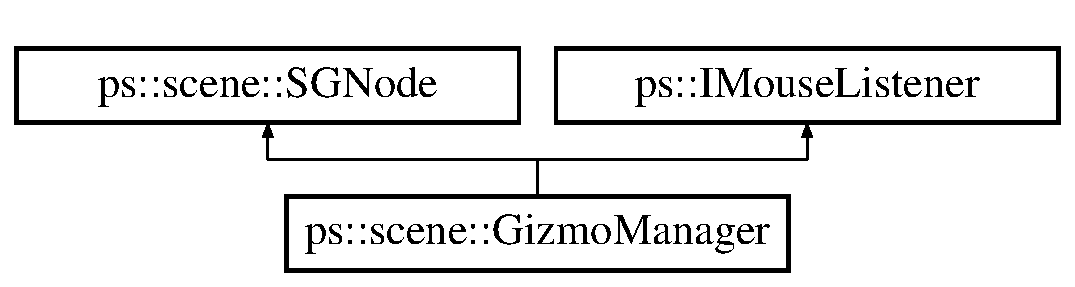
\includegraphics[height=2.000000cm]{classps_1_1scene_1_1GizmoManager}
\end{center}
\end{figure}
\subsection*{Public Member Functions}
\begin{DoxyCompactItemize}
\item 
\hypertarget{classps_1_1scene_1_1GizmoManager_ae6f98a5b2b93b0e95521f374435bf8aa}{}void {\bfseries draw} ()\label{classps_1_1scene_1_1GizmoManager_ae6f98a5b2b93b0e95521f374435bf8aa}

\item 
\hypertarget{classps_1_1scene_1_1GizmoManager_ae01a4723af3246cf01baeb89b9a9d795}{}void {\bfseries timestep} ()\label{classps_1_1scene_1_1GizmoManager_ae01a4723af3246cf01baeb89b9a9d795}

\item 
\hypertarget{classps_1_1scene_1_1GizmoManager_afa9e28718b8b2798508fea0094513960}{}int {\bfseries intersect} (const \hyperlink{classps_1_1base_1_1Ray}{Ray} \&r)\label{classps_1_1scene_1_1GizmoManager_afa9e28718b8b2798508fea0094513960}

\item 
\hypertarget{classps_1_1scene_1_1GizmoManager_a1a6169a881b5e8f7ee418fe9d0cc88a5}{}Gizmo\+Type {\bfseries gizmo\+Type} () const \label{classps_1_1scene_1_1GizmoManager_a1a6169a881b5e8f7ee418fe9d0cc88a5}

\item 
\hypertarget{classps_1_1scene_1_1GizmoManager_abeccebb9b0de86365d133a3e1f729b16}{}Gizmo\+Axis {\bfseries axis} () const \label{classps_1_1scene_1_1GizmoManager_abeccebb9b0de86365d133a3e1f729b16}

\item 
\hypertarget{classps_1_1scene_1_1GizmoManager_a593619fdba423decc8f54d33006fc54a}{}void {\bfseries mouse\+Press} (Mouse\+Button button, Mouse\+Button\+State state, int x, int y) override\label{classps_1_1scene_1_1GizmoManager_a593619fdba423decc8f54d33006fc54a}

\item 
\hypertarget{classps_1_1scene_1_1GizmoManager_af9e7d29589c8cda82f82f1918cfce53d}{}void {\bfseries mouse\+Move} (int x, int y) override\label{classps_1_1scene_1_1GizmoManager_af9e7d29589c8cda82f82f1918cfce53d}

\item 
\hypertarget{classps_1_1scene_1_1GizmoManager_a221c85a888ea684fdfff493a83171e6e}{}void {\bfseries mouse\+Wheel} (Mouse\+Wheel\+Dir dir) override\label{classps_1_1scene_1_1GizmoManager_a221c85a888ea684fdfff493a83171e6e}

\item 
\hypertarget{classps_1_1scene_1_1GizmoManager_a119fd0435fa5b99f4498bbf9b30acbab}{}void {\bfseries set\+Axis} (const \hyperlink{classps_1_1base_1_1Ray}{Ray} \&r)\label{classps_1_1scene_1_1GizmoManager_a119fd0435fa5b99f4498bbf9b30acbab}

\item 
\hypertarget{classps_1_1scene_1_1GizmoManager_aa6eab2f45c4d1c6d776cb8f926beb990}{}void {\bfseries set\+Axis} (Gizmo\+Axis axis)\label{classps_1_1scene_1_1GizmoManager_aa6eab2f45c4d1c6d776cb8f926beb990}

\item 
\hypertarget{classps_1_1scene_1_1GizmoManager_af9660af664d6f389270711ae6b8bbc40}{}void {\bfseries set\+Type} (Gizmo\+Type gtype)\label{classps_1_1scene_1_1GizmoManager_af9660af664d6f389270711ae6b8bbc40}

\item 
\hypertarget{classps_1_1scene_1_1GizmoManager_a22247b7433ab858a3344aa0df2f2489a}{}\hyperlink{classps_1_1scene_1_1GizmoInterface}{Gizmo\+Interface} $\ast$ {\bfseries current} () const \label{classps_1_1scene_1_1GizmoManager_a22247b7433ab858a3344aa0df2f2489a}

\item 
\hypertarget{classps_1_1scene_1_1GizmoManager_af69706acd0759b23b8088b262c1da571}{}void {\bfseries set\+Focused\+Node} (\hyperlink{classps_1_1scene_1_1SGNode}{S\+G\+Node} $\ast$node)\label{classps_1_1scene_1_1GizmoManager_af69706acd0759b23b8088b262c1da571}

\item 
\hypertarget{classps_1_1scene_1_1GizmoManager_a20837fbaf766b0720c1e7dca14c45d84}{}int {\bfseries register\+Client} (\hyperlink{classps_1_1scene_1_1IGizmoListener}{I\+Gizmo\+Listener} $\ast$client)\label{classps_1_1scene_1_1GizmoManager_a20837fbaf766b0720c1e7dca14c45d84}

\item 
\hypertarget{classps_1_1scene_1_1GizmoManager_a70a078236fe4a1ae2356877f49bd1955}{}void {\bfseries unregister\+Client} (int id)\label{classps_1_1scene_1_1GizmoManager_a70a078236fe4a1ae2356877f49bd1955}

\item 
\hypertarget{classps_1_1scene_1_1GizmoManager_af7f46caee5644aba11b40e38f8d0bc8b}{}void {\bfseries cmd\+Translate} (const \hyperlink{classps_1_1base_1_1Vec3}{vec3f} \&increment)\label{classps_1_1scene_1_1GizmoManager_af7f46caee5644aba11b40e38f8d0bc8b}

\item 
\hypertarget{classps_1_1scene_1_1GizmoManager_a3e150b8e51c5584eaee93a1251ef0827}{}void {\bfseries cmd\+Scale} (const \hyperlink{classps_1_1base_1_1Vec3}{vec3f} \&increment)\label{classps_1_1scene_1_1GizmoManager_a3e150b8e51c5584eaee93a1251ef0827}

\item 
\hypertarget{classps_1_1scene_1_1GizmoManager_a51a49044f0e3bca22b2717e8c66b568c}{}void {\bfseries cmd\+Rotate} (const \hyperlink{classps_1_1base_1_1Quaternion}{quatf} \&q)\label{classps_1_1scene_1_1GizmoManager_a51a49044f0e3bca22b2717e8c66b568c}

\item 
\hypertarget{classps_1_1scene_1_1GizmoManager_a00c8994957394b31765cc087fe96351c}{}void {\bfseries cmd\+Rotate} (const \hyperlink{classps_1_1base_1_1Vec3}{vec3f} \&axis, float degree\+Increment)\label{classps_1_1scene_1_1GizmoManager_a00c8994957394b31765cc087fe96351c}

\item 
\hypertarget{classps_1_1scene_1_1GizmoManager_a4118cdc5199d3571d4d84830ba8db6bd}{}bool {\bfseries read\+Config} (const \hyperlink{classps_1_1base_1_1CAString}{Ansi\+Str} \&str\+F\+P=\char`\"{}gizmo.\+ini\char`\"{})\label{classps_1_1scene_1_1GizmoManager_a4118cdc5199d3571d4d84830ba8db6bd}

\item 
\hypertarget{classps_1_1scene_1_1GizmoManager_ad536d72a9044cf766ea37e15d4bd1dfa}{}bool {\bfseries write\+Config} (const \hyperlink{classps_1_1base_1_1CAString}{Ansi\+Str} \&str\+F\+P=\char`\"{}gizmo.\+ini\char`\"{})\label{classps_1_1scene_1_1GizmoManager_ad536d72a9044cf766ea37e15d4bd1dfa}

\end{DoxyCompactItemize}
\subsection*{Static Public Member Functions}
\begin{DoxyCompactItemize}
\item 
\hypertarget{classps_1_1scene_1_1GizmoManager_adabbb5340c1de475e7e0bb25034f95b2}{}static string {\bfseries Axis\+To\+Str} (Gizmo\+Axis axis)\label{classps_1_1scene_1_1GizmoManager_adabbb5340c1de475e7e0bb25034f95b2}

\end{DoxyCompactItemize}
\subsection*{Additional Inherited Members}


\subsection{Detailed Description}
Gizmo Manager controls the U\+I Widgets for sketching, transforming, cutting and poking of deformable models. 

The documentation for this class was generated from the following files\+:\begin{DoxyCompactItemize}
\item 
/\+Users/pourya/\+Desktop/platform/repos/tetcutter/src/scene/gizmo.\+h\item 
/\+Users/pourya/\+Desktop/platform/repos/tetcutter/src/scene/gizmo.\+cpp\end{DoxyCompactItemize}

\hypertarget{classps_1_1scene_1_1GizmoRotate}{}\section{ps\+:\+:scene\+:\+:Gizmo\+Rotate Class Reference}
\label{classps_1_1scene_1_1GizmoRotate}\index{ps\+::scene\+::\+Gizmo\+Rotate@{ps\+::scene\+::\+Gizmo\+Rotate}}
Inheritance diagram for ps\+:\+:scene\+:\+:Gizmo\+Rotate\+:\begin{figure}[H]
\begin{center}
\leavevmode
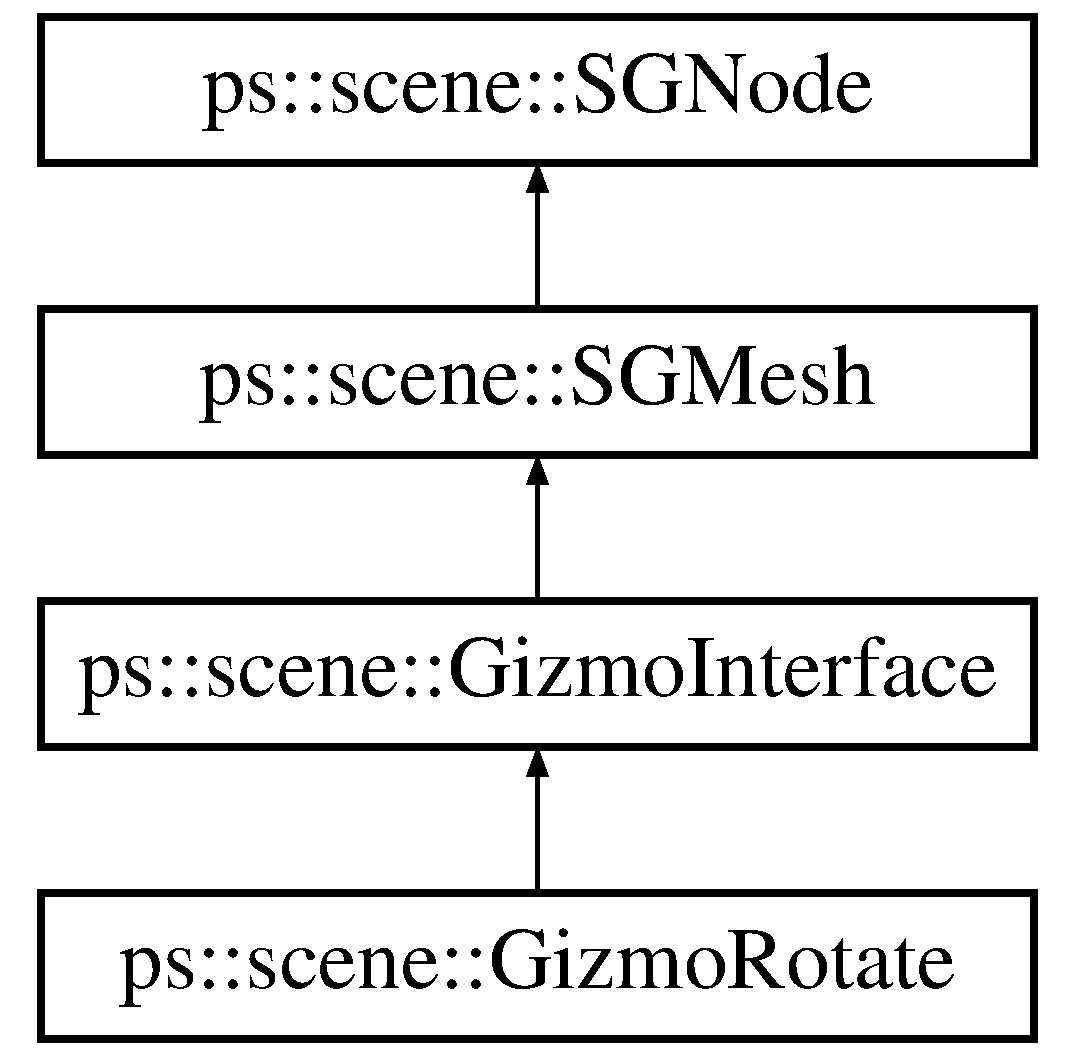
\includegraphics[height=4.000000cm]{classps_1_1scene_1_1GizmoRotate}
\end{center}
\end{figure}
\subsection*{Public Member Functions}
\begin{DoxyCompactItemize}
\item 
\hypertarget{classps_1_1scene_1_1GizmoRotate_a4b5b365a5783c65bf2e2e9ef88c56cfc}{}void {\bfseries draw} ()\label{classps_1_1scene_1_1GizmoRotate_a4b5b365a5783c65bf2e2e9ef88c56cfc}

\item 
\hypertarget{classps_1_1scene_1_1GizmoRotate_aef3baee21c5d540657938c71b6aa42e7}{}int {\bfseries intersect} (const \hyperlink{classps_1_1base_1_1Ray}{Ray} \&r)\label{classps_1_1scene_1_1GizmoRotate_aef3baee21c5d540657938c71b6aa42e7}

\item 
\hypertarget{classps_1_1scene_1_1GizmoRotate_a4fd70a55173d8d4746ffd4968cf4f79c}{}int {\bfseries set\+Axis} (const \hyperlink{classps_1_1base_1_1Ray}{Ray} \&r)\label{classps_1_1scene_1_1GizmoRotate_a4fd70a55173d8d4746ffd4968cf4f79c}

\item 
\hypertarget{classps_1_1scene_1_1GizmoRotate_aeeca97ecfe9fb39c224891e08c940769}{}void {\bfseries rotate} (Gizmo\+Axis axis, float degree)\label{classps_1_1scene_1_1GizmoRotate_aeeca97ecfe9fb39c224891e08c940769}

\end{DoxyCompactItemize}
\subsection*{Protected Member Functions}
\begin{DoxyCompactItemize}
\item 
\hypertarget{classps_1_1scene_1_1GizmoRotate_af2e52ea84e3368f8a47acbd5823acd31}{}void {\bfseries setup} ()\label{classps_1_1scene_1_1GizmoRotate_af2e52ea84e3368f8a47acbd5823acd31}

\end{DoxyCompactItemize}
\subsection*{Additional Inherited Members}


The documentation for this class was generated from the following files\+:\begin{DoxyCompactItemize}
\item 
/\+Users/pourya/\+Desktop/platform/repos/tetcutter/src/scene/gizmo.\+h\item 
/\+Users/pourya/\+Desktop/platform/repos/tetcutter/src/scene/gizmo.\+cpp\end{DoxyCompactItemize}

\hypertarget{classps_1_1scene_1_1GizmoScale}{}\section{ps\+:\+:scene\+:\+:Gizmo\+Scale Class Reference}
\label{classps_1_1scene_1_1GizmoScale}\index{ps\+::scene\+::\+Gizmo\+Scale@{ps\+::scene\+::\+Gizmo\+Scale}}
Inheritance diagram for ps\+:\+:scene\+:\+:Gizmo\+Scale\+:\begin{figure}[H]
\begin{center}
\leavevmode
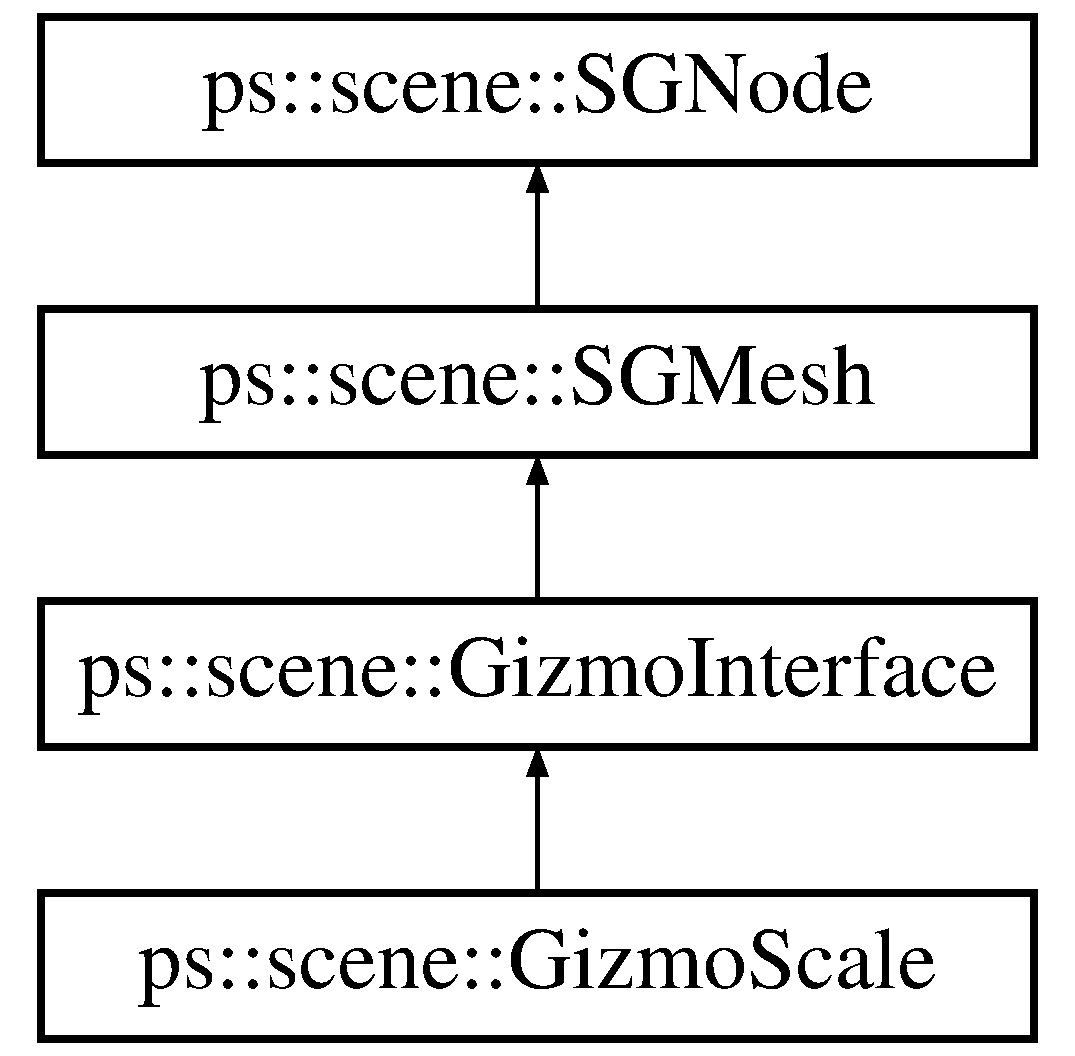
\includegraphics[height=4.000000cm]{classps_1_1scene_1_1GizmoScale}
\end{center}
\end{figure}
\subsection*{Public Member Functions}
\begin{DoxyCompactItemize}
\item 
\hypertarget{classps_1_1scene_1_1GizmoScale_a2c5a8f89a0f2a054147e5798ee4446f8}{}void {\bfseries draw} ()\label{classps_1_1scene_1_1GizmoScale_a2c5a8f89a0f2a054147e5798ee4446f8}

\item 
\hypertarget{classps_1_1scene_1_1GizmoScale_af2c3f0a6992d8498340bef073ea227af}{}int {\bfseries intersect} (const \hyperlink{classps_1_1base_1_1Ray}{Ray} \&r)\label{classps_1_1scene_1_1GizmoScale_af2c3f0a6992d8498340bef073ea227af}

\end{DoxyCompactItemize}
\subsection*{Protected Member Functions}
\begin{DoxyCompactItemize}
\item 
\hypertarget{classps_1_1scene_1_1GizmoScale_a9fefd122b2bb835deec8f125ebea1f14}{}void {\bfseries setup} ()\label{classps_1_1scene_1_1GizmoScale_a9fefd122b2bb835deec8f125ebea1f14}

\end{DoxyCompactItemize}
\subsection*{Additional Inherited Members}


The documentation for this class was generated from the following files\+:\begin{DoxyCompactItemize}
\item 
/\+Users/pourya/\+Desktop/platform/repos/tetcutter/src/scene/gizmo.\+h\item 
/\+Users/pourya/\+Desktop/platform/repos/tetcutter/src/scene/gizmo.\+cpp\end{DoxyCompactItemize}

\hypertarget{classps_1_1scene_1_1GizmoTranslate}{}\section{ps\+:\+:scene\+:\+:Gizmo\+Translate Class Reference}
\label{classps_1_1scene_1_1GizmoTranslate}\index{ps\+::scene\+::\+Gizmo\+Translate@{ps\+::scene\+::\+Gizmo\+Translate}}
Inheritance diagram for ps\+:\+:scene\+:\+:Gizmo\+Translate\+:\begin{figure}[H]
\begin{center}
\leavevmode
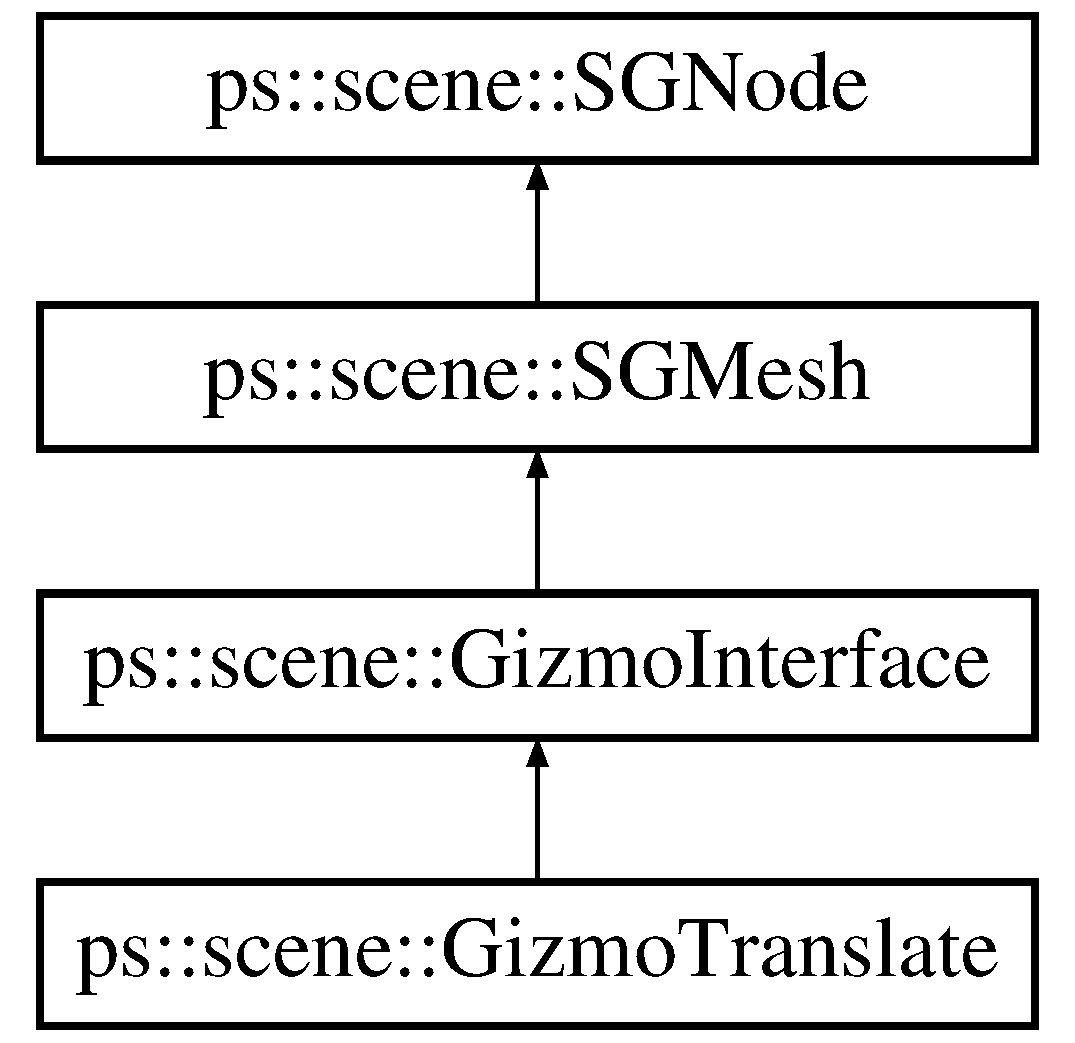
\includegraphics[height=4.000000cm]{classps_1_1scene_1_1GizmoTranslate}
\end{center}
\end{figure}
\subsection*{Public Member Functions}
\begin{DoxyCompactItemize}
\item 
\hypertarget{classps_1_1scene_1_1GizmoTranslate_aca58c171403c76574eee0ea04accf8c5}{}void {\bfseries draw} ()\label{classps_1_1scene_1_1GizmoTranslate_aca58c171403c76574eee0ea04accf8c5}

\item 
\hypertarget{classps_1_1scene_1_1GizmoTranslate_a3c4afe3233bd1733bc8243c048c90ec0}{}int {\bfseries intersect} (const \hyperlink{classps_1_1base_1_1Ray}{Ray} \&r)\label{classps_1_1scene_1_1GizmoTranslate_a3c4afe3233bd1733bc8243c048c90ec0}

\end{DoxyCompactItemize}
\subsection*{Protected Member Functions}
\begin{DoxyCompactItemize}
\item 
\hypertarget{classps_1_1scene_1_1GizmoTranslate_a7604e066324193919e707c0bfbf6de20}{}void {\bfseries setup} ()\label{classps_1_1scene_1_1GizmoTranslate_a7604e066324193919e707c0bfbf6de20}

\end{DoxyCompactItemize}
\subsection*{Additional Inherited Members}


The documentation for this class was generated from the following files\+:\begin{DoxyCompactItemize}
\item 
/\+Users/pourya/\+Desktop/platform/repos/tetcutter/src/scene/gizmo.\+h\item 
/\+Users/pourya/\+Desktop/platform/repos/tetcutter/src/scene/gizmo.\+cpp\end{DoxyCompactItemize}

\hypertarget{classps_1_1opengl_1_1GLBindable}{}\section{ps\+:\+:opengl\+:\+:G\+L\+Bindable Class Reference}
\label{classps_1_1opengl_1_1GLBindable}\index{ps\+::opengl\+::\+G\+L\+Bindable@{ps\+::opengl\+::\+G\+L\+Bindable}}
Inheritance diagram for ps\+:\+:opengl\+:\+:G\+L\+Bindable\+:\begin{figure}[H]
\begin{center}
\leavevmode
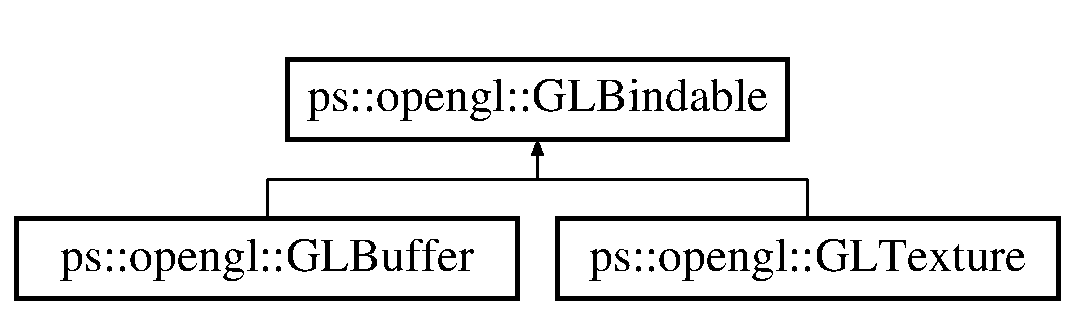
\includegraphics[height=2.000000cm]{classps_1_1opengl_1_1GLBindable}
\end{center}
\end{figure}
\subsection*{Public Member Functions}
\begin{DoxyCompactItemize}
\item 
\hypertarget{classps_1_1opengl_1_1GLBindable_afba8e1354f41b4b403c8c6bc46189644}{}virtual void {\bfseries bind} ()=0\label{classps_1_1opengl_1_1GLBindable_afba8e1354f41b4b403c8c6bc46189644}

\item 
\hypertarget{classps_1_1opengl_1_1GLBindable_acd6f392309e94936dc1d01d146877da4}{}virtual void {\bfseries unbind} ()=0\label{classps_1_1opengl_1_1GLBindable_acd6f392309e94936dc1d01d146877da4}

\end{DoxyCompactItemize}


The documentation for this class was generated from the following files\+:\begin{DoxyCompactItemize}
\item 
/\+Users/pourya/\+Desktop/platform/repos/tetcutter/src/glbackend/glbindable.\+h\item 
/\+Users/pourya/\+Desktop/platform/repos/tetcutter/src/glbackend/glbindable.\+cpp\end{DoxyCompactItemize}

\hypertarget{classps_1_1opengl_1_1GLBuffer}{}\section{ps\+:\+:opengl\+:\+:G\+L\+Buffer Class Reference}
\label{classps_1_1opengl_1_1GLBuffer}\index{ps\+::opengl\+::\+G\+L\+Buffer@{ps\+::opengl\+::\+G\+L\+Buffer}}


{\ttfamily \#include $<$glbuffer.\+h$>$}

Inheritance diagram for ps\+:\+:opengl\+:\+:G\+L\+Buffer\+:\begin{figure}[H]
\begin{center}
\leavevmode
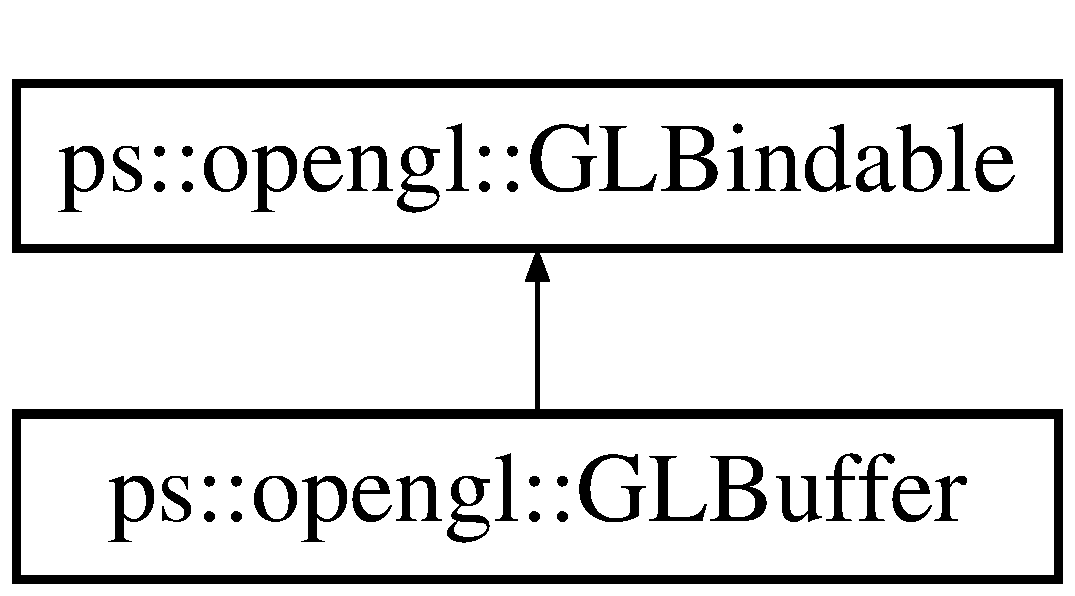
\includegraphics[height=2.000000cm]{classps_1_1opengl_1_1GLBuffer}
\end{center}
\end{figure}
\subsection*{Public Member Functions}
\begin{DoxyCompactItemize}
\item 
\hypertarget{classps_1_1opengl_1_1GLBuffer_a97b5c0b62050c944549757c55ba5c633}{}{\bfseries G\+L\+Buffer} (G\+L\+Buffer\+Type type, int step, int datatype, U32 sz\+Total, const void $\ast$lp\+Data, G\+L\+Buffer\+Usage usage=gbu\+Static\+Draw)\label{classps_1_1opengl_1_1GLBuffer_a97b5c0b62050c944549757c55ba5c633}

\item 
\hypertarget{classps_1_1opengl_1_1GLBuffer_a662528800299731eba4a9d19b7a1624a}{}bool {\bfseries setup} (G\+L\+Buffer\+Type type, int step, int datatype, U32 sz\+Total, const void $\ast$lp\+Data, G\+L\+Buffer\+Usage usage=gbu\+Static\+Draw)\label{classps_1_1opengl_1_1GLBuffer_a662528800299731eba4a9d19b7a1624a}

\item 
\hypertarget{classps_1_1opengl_1_1GLBuffer_afc98042ce97174bd0b732719f74bd841}{}void {\bfseries cleanup} ()\label{classps_1_1opengl_1_1GLBuffer_afc98042ce97174bd0b732719f74bd841}

\item 
\hypertarget{classps_1_1opengl_1_1GLBuffer_af2c0369caeab0038b380a729ec949327}{}void {\bfseries resize} (U32 sz\+Total, const void $\ast$lp\+Data)\label{classps_1_1opengl_1_1GLBuffer_af2c0369caeab0038b380a729ec949327}

\item 
\hypertarget{classps_1_1opengl_1_1GLBuffer_a8781382ead064acb42fdb80392e6b378}{}void {\bfseries bind} ()\label{classps_1_1opengl_1_1GLBuffer_a8781382ead064acb42fdb80392e6b378}

\item 
\hypertarget{classps_1_1opengl_1_1GLBuffer_ad715c58d6b17254c5653dc6c778ff5b5}{}void {\bfseries unbind} ()\label{classps_1_1opengl_1_1GLBuffer_ad715c58d6b17254c5653dc6c778ff5b5}

\item 
\hypertarget{classps_1_1opengl_1_1GLBuffer_aaf21827dfc8a3f66b5a61d7881a32745}{}void {\bfseries draw\+Elements} (int face\+Mode, int ct\+Elements)\label{classps_1_1opengl_1_1GLBuffer_aaf21827dfc8a3f66b5a61d7881a32745}

\item 
bool \hyperlink{classps_1_1opengl_1_1GLBuffer_a0341f4338ac221c8adab5106fd6494a6}{modify} (U32 offset, U32 sz\+Total, const void $\ast$lp\+Data)
\item 
\hypertarget{classps_1_1opengl_1_1GLBuffer_a50eb260cfbb1faa3cc362174dce1bf92}{}bool {\bfseries read\+Back} (U32 sz\+Out\+Buffer, void $\ast$lp\+Out\+Buffer) const \label{classps_1_1opengl_1_1GLBuffer_a50eb260cfbb1faa3cc362174dce1bf92}

\item 
\hypertarget{classps_1_1opengl_1_1GLBuffer_a1b924a3d13f057c6ca7d6db933e6c8d9}{}bool {\bfseries is\+Valid} () const \label{classps_1_1opengl_1_1GLBuffer_a1b924a3d13f057c6ca7d6db933e6c8d9}

\item 
\hypertarget{classps_1_1opengl_1_1GLBuffer_a0e18faa846c0bfc9cda2da5121c8cd39}{}int {\bfseries step} () const \label{classps_1_1opengl_1_1GLBuffer_a0e18faa846c0bfc9cda2da5121c8cd39}

\item 
\hypertarget{classps_1_1opengl_1_1GLBuffer_aebe3201267c865d710beb8986d9e991c}{}U32 {\bfseries size} () const \label{classps_1_1opengl_1_1GLBuffer_aebe3201267c865d710beb8986d9e991c}

\item 
\hypertarget{classps_1_1opengl_1_1GLBuffer_adc8dcb0f7e428fd599b5010c7b1e8e28}{}U32 {\bfseries handle} () const \label{classps_1_1opengl_1_1GLBuffer_adc8dcb0f7e428fd599b5010c7b1e8e28}

\item 
\hypertarget{classps_1_1opengl_1_1GLBuffer_ab831ebea567f9b34967d635e1b1a606b}{}G\+L\+Buffer\+Type {\bfseries type} () const \label{classps_1_1opengl_1_1GLBuffer_ab831ebea567f9b34967d635e1b1a606b}

\end{DoxyCompactItemize}
\subsection*{Protected Member Functions}
\begin{DoxyCompactItemize}
\item 
\hypertarget{classps_1_1opengl_1_1GLBuffer_ae786850093e546eaceffe6e9e90851a6}{}void {\bfseries init} ()\label{classps_1_1opengl_1_1GLBuffer_ae786850093e546eaceffe6e9e90851a6}

\end{DoxyCompactItemize}


\subsection{Detailed Description}
Open\+G\+L Memory Buffer 

\subsection{Member Function Documentation}
\hypertarget{classps_1_1opengl_1_1GLBuffer_a0341f4338ac221c8adab5106fd6494a6}{}\index{ps\+::opengl\+::\+G\+L\+Buffer@{ps\+::opengl\+::\+G\+L\+Buffer}!modify@{modify}}
\index{modify@{modify}!ps\+::opengl\+::\+G\+L\+Buffer@{ps\+::opengl\+::\+G\+L\+Buffer}}
\subsubsection[{modify(\+U32 offset, U32 sz\+Total, const void $\ast$lp\+Data)}]{\setlength{\rightskip}{0pt plus 5cm}bool G\+L\+Buffer\+::modify (
\begin{DoxyParamCaption}
\item[{U32}]{offset, }
\item[{U32}]{sz\+Total, }
\item[{const void $\ast$}]{lp\+Data}
\end{DoxyParamCaption}
)}\label{classps_1_1opengl_1_1GLBuffer_a0341f4338ac221c8adab5106fd6494a6}
Modifies the buffer for changes 

The documentation for this class was generated from the following files\+:\begin{DoxyCompactItemize}
\item 
/\+Users/pourya/\+Desktop/platform/repos/tetcutter/src/glbackend/glbuffer.\+h\item 
/\+Users/pourya/\+Desktop/platform/repos/tetcutter/src/glbackend/glbuffer.\+cpp\end{DoxyCompactItemize}

\hypertarget{classps_1_1opengl_1_1GLMesh}{}\section{ps\+:\+:opengl\+:\+:G\+L\+Mesh Class Reference}
\label{classps_1_1opengl_1_1GLMesh}\index{ps\+::opengl\+::\+G\+L\+Mesh@{ps\+::opengl\+::\+G\+L\+Mesh}}


{\ttfamily \#include $<$glmeshbuffer.\+h$>$}

\subsection*{Public Member Functions}
\begin{DoxyCompactItemize}
\item 
\hypertarget{classps_1_1opengl_1_1GLMesh_a8f24ba9a17b57f5a92aed63ae049dc68}{}void {\bfseries setup\+Vertex\+Attribs} (const vector$<$ float $>$ \&arr\+Attribs, int step=3, G\+L\+Buffer\+Type attrib\+Kind=gbt\+Position)\label{classps_1_1opengl_1_1GLMesh_a8f24ba9a17b57f5a92aed63ae049dc68}

\item 
\hypertarget{classps_1_1opengl_1_1GLMesh_a6e530628b25140366b442e314cf701a0}{}void {\bfseries setup\+Per\+Vertex\+Color} (const \hyperlink{classps_1_1base_1_1Vec4}{vec4f} \&color, U32 ct\+Vertices, int step=4)\label{classps_1_1opengl_1_1GLMesh_a6e530628b25140366b442e314cf701a0}

\item 
\hypertarget{classps_1_1opengl_1_1GLMesh_a3d9fb6b505824b6b5fde7eaa56ecf219}{}void {\bfseries setup\+Face\+Indices} (U32 ct\+Face\+Elements, G\+L\+Face\+Type face\+Mode=ft\+Triangles)\label{classps_1_1opengl_1_1GLMesh_a3d9fb6b505824b6b5fde7eaa56ecf219}

\item 
\hypertarget{classps_1_1opengl_1_1GLMesh_a4b980b340dfc1c734c8e986fbaf007ad}{}void {\bfseries setup\+Face\+Index\+Buffer} (const vector$<$ U32 $>$ \&arr\+Index, G\+L\+Face\+Type face\+Mode=ft\+Triangles)\label{classps_1_1opengl_1_1GLMesh_a4b980b340dfc1c734c8e986fbaf007ad}

\item 
\hypertarget{classps_1_1opengl_1_1GLMesh_a2bb37434c68fe755015c1716b3d51457}{}{\footnotesize template$<$typename T $>$ }\\void {\bfseries setup\+Vertex\+Attribs\+T} (int gl\+Type, const vector$<$ T $>$ \&arr\+Attribs, int step, G\+L\+Buffer\+Type attrib\+Kind, G\+L\+Buffer\+Usage usage=gbu\+Static\+Draw)\label{classps_1_1opengl_1_1GLMesh_a2bb37434c68fe755015c1716b3d51457}

\item 
\hypertarget{classps_1_1opengl_1_1GLMesh_a2b8cad1819d0ae4f4fc902f2c202d98e}{}{\footnotesize template$<$typename T $>$ }\\void {\bfseries setup\+Per\+Vertex\+Color\+T} (int gl\+Type, const \hyperlink{classps_1_1base_1_1Color}{Color} \&color, U32 ct\+Vertices, int step=4)\label{classps_1_1opengl_1_1GLMesh_a2b8cad1819d0ae4f4fc902f2c202d98e}

\item 
\hypertarget{classps_1_1opengl_1_1GLMesh_a87a022a8d31a673b336d2f0271fe0cf7}{}{\footnotesize template$<$typename T $>$ }\\void {\bfseries setup\+Face\+Index\+Buffer\+T} (int gl\+Type, const vector$<$ T $>$ \&arr\+Index, G\+L\+Face\+Type face\+Mode=ft\+Triangles)\label{classps_1_1opengl_1_1GLMesh_a87a022a8d31a673b336d2f0271fe0cf7}

\item 
\hypertarget{classps_1_1opengl_1_1GLMesh_a86420e2cf6d18d31ede0367fbfd15400}{}{\footnotesize template$<$typename T $>$ }\\bool {\bfseries readback\+Face\+Buffer} (int gl\+Type, U32 \&count, vector$<$ T $>$ \&indices) const \label{classps_1_1opengl_1_1GLMesh_a86420e2cf6d18d31ede0367fbfd15400}

\item 
\hypertarget{classps_1_1opengl_1_1GLMesh_a200089ac29a7eb872897e7978ae7e2e1}{}bool {\bfseries wireframe\+Mode} () const \label{classps_1_1opengl_1_1GLMesh_a200089ac29a7eb872897e7978ae7e2e1}

\item 
\hypertarget{classps_1_1opengl_1_1GLMesh_a0ac5b90c2581ca7a9394c641a34ca870}{}virtual void {\bfseries set\+Wire\+Frame\+Mode} (bool mode)\label{classps_1_1opengl_1_1GLMesh_a0ac5b90c2581ca7a9394c641a34ca870}

\item 
\hypertarget{classps_1_1opengl_1_1GLMesh_a9e21781ca568ff2b4a9825c3e91032f1}{}int {\bfseries face\+Mode} () const \label{classps_1_1opengl_1_1GLMesh_a9e21781ca568ff2b4a9825c3e91032f1}

\item 
\hypertarget{classps_1_1opengl_1_1GLMesh_abe2bbe4a607cb98faa8c8d62acf6aa83}{}void {\bfseries set\+Face\+Mode} (G\+L\+Face\+Type face\+Mode)\label{classps_1_1opengl_1_1GLMesh_abe2bbe4a607cb98faa8c8d62acf6aa83}

\item 
\hypertarget{classps_1_1opengl_1_1GLMesh_a4a30230bd828ec4661911320c398e6d5}{}void {\bfseries set\+Face\+Elements\+Count} (U32 ct\+Face\+Elems)\label{classps_1_1opengl_1_1GLMesh_a4a30230bd828ec4661911320c398e6d5}

\item 
\hypertarget{classps_1_1opengl_1_1GLMesh_a89d62a3f483d6d91448af9905a766a3c}{}U32 {\bfseries count\+Vertices} () const \label{classps_1_1opengl_1_1GLMesh_a89d62a3f483d6d91448af9905a766a3c}

\item 
\hypertarget{classps_1_1opengl_1_1GLMesh_ad5b9d09d188605c4684eb5e2111a7980}{}U32 {\bfseries count\+Faces} () const \label{classps_1_1opengl_1_1GLMesh_ad5b9d09d188605c4684eb5e2111a7980}

\item 
\hypertarget{classps_1_1opengl_1_1GLMesh_a898aeb13042ef88ca1ab8e305af87688}{}bool {\bfseries is\+Buffer\+Valid} (G\+L\+Buffer\+Type attrib\+Type=gbt\+Position) const \label{classps_1_1opengl_1_1GLMesh_a898aeb13042ef88ca1ab8e305af87688}

\item 
\hypertarget{classps_1_1opengl_1_1GLMesh_a3e99f6d363d2a4b9b289e23d778d23de}{}const \hyperlink{classps_1_1opengl_1_1GLBuffer}{G\+L\+Buffer} $\ast$ {\bfseries const\+\_\+buffer} (G\+L\+Buffer\+Type attrib\+Type) const \label{classps_1_1opengl_1_1GLMesh_a3e99f6d363d2a4b9b289e23d778d23de}

\item 
\hypertarget{classps_1_1opengl_1_1GLMesh_a58b9119add26f74ae0008bcd1af44238}{}\hyperlink{classps_1_1opengl_1_1GLBuffer}{G\+L\+Buffer} $\ast$ {\bfseries buffer} (G\+L\+Buffer\+Type attrib\+Type)\label{classps_1_1opengl_1_1GLMesh_a58b9119add26f74ae0008bcd1af44238}

\item 
\hypertarget{classps_1_1opengl_1_1GLMesh_a57e0d0fc417bbda5eef7013eb4542ad5}{}bool {\bfseries modify\+Vertex\+Buffer} (U32 offset, U32 sz\+Total, const void $\ast$lp\+Data)\label{classps_1_1opengl_1_1GLMesh_a57e0d0fc417bbda5eef7013eb4542ad5}

\item 
\hypertarget{classps_1_1opengl_1_1GLMesh_aa59a7234a8e89d6aee84758ab50874ac}{}void {\bfseries clear\+All\+Buffers} ()\label{classps_1_1opengl_1_1GLMesh_aa59a7234a8e89d6aee84758ab50874ac}

\item 
\hypertarget{classps_1_1opengl_1_1GLMesh_a135e8f9a8c85b4b99ca59acf4246a0bd}{}virtual void {\bfseries draw} ()\label{classps_1_1opengl_1_1GLMesh_a135e8f9a8c85b4b99ca59acf4246a0bd}

\end{DoxyCompactItemize}
\subsection*{Static Public Member Functions}
\begin{DoxyCompactItemize}
\item 
\hypertarget{classps_1_1opengl_1_1GLMesh_a187c41a36f2b8e4b08406796e436f228}{}static int {\bfseries Face\+Step\+Size\+From\+Mode} (G\+L\+Face\+Type face)\label{classps_1_1opengl_1_1GLMesh_a187c41a36f2b8e4b08406796e436f228}

\item 
\hypertarget{classps_1_1opengl_1_1GLMesh_a608789c7fc06893303139efd29d39865}{}static \hyperlink{classps_1_1opengl_1_1GLMesh}{G\+L\+Mesh} $\ast$ {\bfseries Prepare\+Mesh\+Buffer\+For\+Drawing\+Normals} (float len, U32 ct\+Vertices, U32 fstep, const vector$<$ float $>$ \&arr\+Vertices, const vector$<$ float $>$ \&arr\+Normals)\label{classps_1_1opengl_1_1GLMesh_a608789c7fc06893303139efd29d39865}

\item 
\hypertarget{classps_1_1opengl_1_1GLMesh_a089b4ed0bc4dde11f9eed688cb9123cb}{}static U32 {\bfseries Convert\+Float4\+To\+Float3} (const vector$<$ float $>$ \&arr\+In\+Float4, vector$<$ float $>$ \&arr\+Out\+Float3)\label{classps_1_1opengl_1_1GLMesh_a089b4ed0bc4dde11f9eed688cb9123cb}

\item 
\hypertarget{classps_1_1opengl_1_1GLMesh_a0f29f354fa6a2cbbdc56b9386c261570}{}static U32 {\bfseries Convert\+Float3\+To\+Float4} (const vector$<$ float $>$ \&arr\+In\+Float3, vector$<$ float $>$ \&arr\+Out\+Float4)\label{classps_1_1opengl_1_1GLMesh_a0f29f354fa6a2cbbdc56b9386c261570}

\end{DoxyCompactItemize}
\subsection*{Protected Member Functions}
\begin{DoxyCompactItemize}
\item 
\hypertarget{classps_1_1opengl_1_1GLMesh_a81b350e932dc71633a846b90537b12bd}{}virtual void {\bfseries cleanup} ()\label{classps_1_1opengl_1_1GLMesh_a81b350e932dc71633a846b90537b12bd}

\item 
\hypertarget{classps_1_1opengl_1_1GLMesh_a94b124096bb621f00db163240a08aa6d}{}void {\bfseries init} ()\label{classps_1_1opengl_1_1GLMesh_a94b124096bb621f00db163240a08aa6d}

\end{DoxyCompactItemize}
\subsection*{Protected Attributes}
\begin{DoxyCompactItemize}
\item 
\hypertarget{classps_1_1opengl_1_1GLMesh_adb9804b448f18205223f146a5e064a44}{}\hyperlink{classps_1_1opengl_1_1GLBuffer}{G\+L\+Buffer} {\bfseries m\+\_\+gmb\+Color}\label{classps_1_1opengl_1_1GLMesh_adb9804b448f18205223f146a5e064a44}

\item 
\hypertarget{classps_1_1opengl_1_1GLMesh_a5d995d43b18c65b6802e1f130c03342f}{}\hyperlink{classps_1_1opengl_1_1GLBuffer}{G\+L\+Buffer} {\bfseries m\+\_\+gmb\+Normal}\label{classps_1_1opengl_1_1GLMesh_a5d995d43b18c65b6802e1f130c03342f}

\item 
\hypertarget{classps_1_1opengl_1_1GLMesh_a02f100c270af80f1bded959002b9129d}{}\hyperlink{classps_1_1opengl_1_1GLBuffer}{G\+L\+Buffer} {\bfseries m\+\_\+gmb\+Vertex}\label{classps_1_1opengl_1_1GLMesh_a02f100c270af80f1bded959002b9129d}

\item 
\hypertarget{classps_1_1opengl_1_1GLMesh_abce0f3ae38f6f08ece044fa7f9cd61b6}{}\hyperlink{classps_1_1opengl_1_1GLBuffer}{G\+L\+Buffer} {\bfseries m\+\_\+gmb\+Texcoord}\label{classps_1_1opengl_1_1GLMesh_abce0f3ae38f6f08ece044fa7f9cd61b6}

\item 
\hypertarget{classps_1_1opengl_1_1GLMesh_a0df8c5529e98723c90e5ce571e8dd63a}{}\hyperlink{classps_1_1opengl_1_1GLBuffer}{G\+L\+Buffer} {\bfseries m\+\_\+gmb\+Faces}\label{classps_1_1opengl_1_1GLMesh_a0df8c5529e98723c90e5ce571e8dd63a}

\item 
\hypertarget{classps_1_1opengl_1_1GLMesh_ad1ada023264e3d8db3ae5f77b680761b}{}vector$<$ \hyperlink{classps_1_1opengl_1_1GLBuffer}{G\+L\+Buffer} $\ast$ $>$ {\bfseries m\+\_\+v\+Buffers}\label{classps_1_1opengl_1_1GLMesh_ad1ada023264e3d8db3ae5f77b680761b}

\item 
\hypertarget{classps_1_1opengl_1_1GLMesh_a68d03da4c677851eb0162b7679632bc1}{}bool {\bfseries m\+\_\+b\+Wire\+Frame}\label{classps_1_1opengl_1_1GLMesh_a68d03da4c677851eb0162b7679632bc1}

\item 
\hypertarget{classps_1_1opengl_1_1GLMesh_aaa201d02fa949c18e1c18e25ab72b3da}{}int {\bfseries m\+\_\+face\+Mode}\label{classps_1_1opengl_1_1GLMesh_aaa201d02fa949c18e1c18e25ab72b3da}

\item 
\hypertarget{classps_1_1opengl_1_1GLMesh_ab102495ef716b8a6ff7957893129a5c5}{}U32 {\bfseries m\+\_\+ct\+Face\+Elements}\label{classps_1_1opengl_1_1GLMesh_ab102495ef716b8a6ff7957893129a5c5}

\item 
\hypertarget{classps_1_1opengl_1_1GLMesh_a79c299144f34193014ed9b8132b7b005}{}U32 {\bfseries m\+\_\+ct\+Vertices}\label{classps_1_1opengl_1_1GLMesh_a79c299144f34193014ed9b8132b7b005}

\end{DoxyCompactItemize}


\subsection{Detailed Description}
Synopsis\+: G\+L\+Mesh\+Buffer Simplifies drawing geometries using G\+P\+U Buffers. Types of buffer objects are\+: Vertex, Color, Tex\+Coord, Normal and Index 

The documentation for this class was generated from the following files\+:\begin{DoxyCompactItemize}
\item 
/\+Users/pourya/\+Desktop/platform/repos/tetcutter/src/glbackend/glmeshbuffer.\+h\item 
/\+Users/pourya/\+Desktop/platform/repos/tetcutter/src/glbackend/glmeshbuffer.\+cpp\end{DoxyCompactItemize}

\hypertarget{classps_1_1opengl_1_1GLScreen}{}\section{ps\+:\+:opengl\+:\+:G\+L\+Screen Class Reference}
\label{classps_1_1opengl_1_1GLScreen}\index{ps\+::opengl\+::\+G\+L\+Screen@{ps\+::opengl\+::\+G\+L\+Screen}}


{\ttfamily \#include $<$glscreen.\+h$>$}

\subsection*{Public Member Functions}
\begin{DoxyCompactItemize}
\item 
\hypertarget{classps_1_1opengl_1_1GLScreen_a20ea8ab3fe637a71fd6a322e8c9a9e57}{}{\bfseries G\+L\+Screen} (int argc, char $\ast$argv\mbox{[}$\,$\mbox{]})\label{classps_1_1opengl_1_1GLScreen_a20ea8ab3fe637a71fd6a322e8c9a9e57}

\item 
\hypertarget{classps_1_1opengl_1_1GLScreen_ad1118a7645d4cfc1e15a2895f0d242ec}{}{\bfseries G\+L\+Screen} (int argc, char $\ast$argv\mbox{[}$\,$\mbox{]}, int w, int h, const char $\ast$title)\label{classps_1_1opengl_1_1GLScreen_ad1118a7645d4cfc1e15a2895f0d242ec}

\item 
\hypertarget{classps_1_1opengl_1_1GLScreen_afcba16784a6867bf43cdf1aa852103dc}{}virtual void {\bfseries draw} ()\label{classps_1_1opengl_1_1GLScreen_afcba16784a6867bf43cdf1aa852103dc}

\item 
\hypertarget{classps_1_1opengl_1_1GLScreen_a3f80cbf7d871dc79c8ddb933bc3574d0}{}virtual void {\bfseries resize} (int w, int h)\label{classps_1_1opengl_1_1GLScreen_a3f80cbf7d871dc79c8ddb933bc3574d0}

\item 
\hypertarget{classps_1_1opengl_1_1GLScreen_a055e9c854630528dc49842fceba4fcc3}{}virtual void {\bfseries special\+Key} (int key, int x, int y)=0\label{classps_1_1opengl_1_1GLScreen_a055e9c854630528dc49842fceba4fcc3}

\item 
\hypertarget{classps_1_1opengl_1_1GLScreen_a1671b55a82d64fb49173b859444842cd}{}virtual void {\bfseries normal\+Key} (unsigned char key, int x, int y)=0\label{classps_1_1opengl_1_1GLScreen_a1671b55a82d64fb49173b859444842cd}

\item 
\hypertarget{classps_1_1opengl_1_1GLScreen_aee7a1570a8838d31d7f65e2a370e8970}{}virtual void {\bfseries close} ()\label{classps_1_1opengl_1_1GLScreen_aee7a1570a8838d31d7f65e2a370e8970}

\end{DoxyCompactItemize}
\subsection*{Protected Member Functions}
\begin{DoxyCompactItemize}
\item 
\hypertarget{classps_1_1opengl_1_1GLScreen_a484a950f8c1c67987ac3360774abfb9e}{}void {\bfseries init} (int argc, char $\ast$argv\mbox{[}$\,$\mbox{]})\label{classps_1_1opengl_1_1GLScreen_a484a950f8c1c67987ac3360774abfb9e}

\end{DoxyCompactItemize}


\subsection{Detailed Description}
synopsis\+: Screen for the main 3\+D App 

The documentation for this class was generated from the following files\+:\begin{DoxyCompactItemize}
\item 
/\+Users/pourya/\+Desktop/platform/repos/tetcutter/src/glbackend/glscreen.\+h\item 
/\+Users/pourya/\+Desktop/platform/repos/tetcutter/src/glbackend/glscreen.\+cpp\end{DoxyCompactItemize}

\hypertarget{classps_1_1opengl_1_1GLShader}{}\section{ps\+:\+:opengl\+:\+:G\+L\+Shader Class Reference}
\label{classps_1_1opengl_1_1GLShader}\index{ps\+::opengl\+::\+G\+L\+Shader@{ps\+::opengl\+::\+G\+L\+Shader}}
\subsection*{Classes}
\begin{DoxyCompactItemize}
\item 
struct \hyperlink{structps_1_1opengl_1_1GLShader_1_1VARPROP}{V\+A\+R\+P\+R\+O\+P}
\end{DoxyCompactItemize}
\subsection*{Public Types}
\begin{DoxyCompactItemize}
\item 
\hypertarget{classps_1_1opengl_1_1GLShader_a8d6d57f75b21d839dcb2096312a46d7d}{}enum {\bfseries Shader\+Type} \{ {\bfseries st\+Vertex} = 0, 
{\bfseries st\+Fragment} = 1, 
{\bfseries st\+Geometry} = 2
 \}\label{classps_1_1opengl_1_1GLShader_a8d6d57f75b21d839dcb2096312a46d7d}

\item 
\hypertarget{classps_1_1opengl_1_1GLShader_af769c94af2bda54e8c9bd62eb744df6c}{}enum {\bfseries V\+A\+R\+U\+S\+A\+G\+E} \{ {\bfseries vu\+Attribute}, 
{\bfseries vu\+Uniform}
 \}\label{classps_1_1opengl_1_1GLShader_af769c94af2bda54e8c9bd62eb744df6c}

\item 
\hypertarget{classps_1_1opengl_1_1GLShader_ae33fd492bfa6b1cf991ed87ddcd55f46}{}enum {\bfseries V\+A\+R\+P\+R\+E\+C\+I\+S\+I\+O\+N} \{ {\bfseries vp\+Low}, 
{\bfseries vp\+Medium}, 
{\bfseries vp\+High}, 
{\bfseries vp\+Undefined}
 \}\label{classps_1_1opengl_1_1GLShader_ae33fd492bfa6b1cf991ed87ddcd55f46}

\end{DoxyCompactItemize}
\subsection*{Public Member Functions}
\begin{DoxyCompactItemize}
\item 
\hypertarget{classps_1_1opengl_1_1GLShader_aec8a882e9b10c451769bbbc05fa7db6c}{}{\bfseries G\+L\+Shader} (const char $\ast$psz\+Vertex\+Shader, const char $\ast$psz\+Fragment\+Shader, const char $\ast$psz\+Geometry\+Shader=N\+U\+L\+L)\label{classps_1_1opengl_1_1GLShader_aec8a882e9b10c451769bbbc05fa7db6c}

\item 
\hypertarget{classps_1_1opengl_1_1GLShader_ad8c7835468468206aed1003fa2102c3a}{}void {\bfseries init} ()\label{classps_1_1opengl_1_1GLShader_ad8c7835468468206aed1003fa2102c3a}

\item 
\hypertarget{classps_1_1opengl_1_1GLShader_af3b31be55cd7014586268da6187ae4ab}{}int {\bfseries get\+Uniform\+Location} (const char $\ast$chr\+Uniform\+Name)\label{classps_1_1opengl_1_1GLShader_af3b31be55cd7014586268da6187ae4ab}

\item 
\hypertarget{classps_1_1opengl_1_1GLShader_ad5551ce31a6a3cef1d34b673c8c9d43a}{}void {\bfseries set\+Uniform} (int id\+Loc, const \hyperlink{classps_1_1base_1_1Vec4}{vec4f} \&v)\label{classps_1_1opengl_1_1GLShader_ad5551ce31a6a3cef1d34b673c8c9d43a}

\item 
\hypertarget{classps_1_1opengl_1_1GLShader_abd9fbdc173cf3aaaa83d1e61fc636bac}{}void {\bfseries set\+Uniform} (int id\+Loc, const \hyperlink{classps_1_1base_1_1Vec3}{vec3f} \&v)\label{classps_1_1opengl_1_1GLShader_abd9fbdc173cf3aaaa83d1e61fc636bac}

\item 
\hypertarget{classps_1_1opengl_1_1GLShader_a43fada3ffc1f35b513d44b2cd56a9bbf}{}void {\bfseries set\+Uniform} (int id\+Loc, const \hyperlink{classps_1_1base_1_1Vec2}{vec2f} \&v)\label{classps_1_1opengl_1_1GLShader_a43fada3ffc1f35b513d44b2cd56a9bbf}

\item 
\hypertarget{classps_1_1opengl_1_1GLShader_abbf948b374f5c24b1b8cdb8abbfa5c82}{}void {\bfseries set\+Uniform} (int id\+Loc, float f)\label{classps_1_1opengl_1_1GLShader_abbf948b374f5c24b1b8cdb8abbfa5c82}

\item 
\hypertarget{classps_1_1opengl_1_1GLShader_ac835a8fc64ba683fd919ecbab15b5218}{}void {\bfseries set\+Uniform1i} (int id\+Loc, int i)\label{classps_1_1opengl_1_1GLShader_ac835a8fc64ba683fd919ecbab15b5218}

\item 
\hypertarget{classps_1_1opengl_1_1GLShader_afdff2210c6029c0dc900cbec3e0f69bb}{}int {\bfseries get\+Attrib\+Location} (const char $\ast$chr\+Attrib\+Name)\label{classps_1_1opengl_1_1GLShader_afdff2210c6029c0dc900cbec3e0f69bb}

\item 
\hypertarget{classps_1_1opengl_1_1GLShader_a8fb24f449ca7a386647490eed4049823}{}bool {\bfseries set\+Attrib\+Location} (const char $\ast$chr\+Attrib\+Name, int idx\+Loc)\label{classps_1_1opengl_1_1GLShader_a8fb24f449ca7a386647490eed4049823}

\item 
\hypertarget{classps_1_1opengl_1_1GLShader_ae4c983ad63647d383826aa2be6f49881}{}U32 {\bfseries program} () const \label{classps_1_1opengl_1_1GLShader_ae4c983ad63647d383826aa2be6f49881}

\item 
\hypertarget{classps_1_1opengl_1_1GLShader_a774ba825995a749a8ea646abbc06f9c3}{}bool {\bfseries is\+Compiled} () const \label{classps_1_1opengl_1_1GLShader_a774ba825995a749a8ea646abbc06f9c3}

\item 
\hypertarget{classps_1_1opengl_1_1GLShader_add669d3fceee51498c58a813d89aad7d}{}bool {\bfseries is\+Running} () const \label{classps_1_1opengl_1_1GLShader_add669d3fceee51498c58a813d89aad7d}

\item 
\hypertarget{classps_1_1opengl_1_1GLShader_a8ff87e8e546a08f941bb7513e4a0e543}{}bool {\bfseries is\+Ready\+To\+Run} ()\label{classps_1_1opengl_1_1GLShader_a8ff87e8e546a08f941bb7513e4a0e543}

\item 
\hypertarget{classps_1_1opengl_1_1GLShader_ace4970f8e75f570375e7c7047280a8ee}{}int {\bfseries compile\+From\+File} (const \hyperlink{classps_1_1base_1_1CAString}{Ansi\+Str} \&str\+Vertex\+Shader\+F\+P, const \hyperlink{classps_1_1base_1_1CAString}{Ansi\+Str} \&str\+Fragment\+Shader\+F\+P)\label{classps_1_1opengl_1_1GLShader_ace4970f8e75f570375e7c7047280a8ee}

\item 
\hypertarget{classps_1_1opengl_1_1GLShader_adc66bc2de296f25005935a8166a308ac}{}int {\bfseries compile\+From\+File} (const \hyperlink{classps_1_1base_1_1CAString}{Ansi\+Str} \&str\+Vertex\+Shader\+F\+P, const \hyperlink{classps_1_1base_1_1CAString}{Ansi\+Str} \&str\+Fragment\+Shader\+F\+P, const \hyperlink{classps_1_1base_1_1CAString}{Ansi\+Str} \&str\+Geometry\+Shader\+F\+P)\label{classps_1_1opengl_1_1GLShader_adc66bc2de296f25005935a8166a308ac}

\item 
\hypertarget{classps_1_1opengl_1_1GLShader_a11725e81ad0db66da45f35855b6863ef}{}int {\bfseries compile\+Code} (const char $\ast$v\+Shader\+Code, const char $\ast$v\+Fragment\+Code, const char $\ast$v\+Geometry\+Code=N\+U\+L\+L)\label{classps_1_1opengl_1_1GLShader_a11725e81ad0db66da45f35855b6863ef}

\item 
\hypertarget{classps_1_1opengl_1_1GLShader_a308db5f8c499b1458dd69fbba785feaf}{}bool {\bfseries load\+Binary\+Program} (const char $\ast$Filename, U32 \&Program\+Object\+I\+D)\label{classps_1_1opengl_1_1GLShader_a308db5f8c499b1458dd69fbba785feaf}

\item 
\hypertarget{classps_1_1opengl_1_1GLShader_ab2b3d082fb4bb90dec038939b9d18665}{}bool {\bfseries save\+Binary\+Program} (const char $\ast$Filename, U32 \&Program\+Object\+I\+D)\label{classps_1_1opengl_1_1GLShader_ab2b3d082fb4bb90dec038939b9d18665}

\item 
\hypertarget{classps_1_1opengl_1_1GLShader_a29f8c5924cb221d435bf2ee65caa2aef}{}void {\bfseries start} ()\label{classps_1_1opengl_1_1GLShader_a29f8c5924cb221d435bf2ee65caa2aef}

\item 
\hypertarget{classps_1_1opengl_1_1GLShader_a42762e0f509a31f35e401aac89d1a7de}{}void {\bfseries stop} ()\label{classps_1_1opengl_1_1GLShader_a42762e0f509a31f35e401aac89d1a7de}

\end{DoxyCompactItemize}
\subsection*{Static Public Member Functions}
\begin{DoxyCompactItemize}
\item 
\hypertarget{classps_1_1opengl_1_1GLShader_ad15d47f41618f1c4ec5fd2c6b725768a}{}static bool {\bfseries is\+Binary\+Shader\+Supported} ()\label{classps_1_1opengl_1_1GLShader_ad15d47f41618f1c4ec5fd2c6b725768a}

\item 
\hypertarget{classps_1_1opengl_1_1GLShader_ad1ca02f4cc5015f8580a76bd44c3ae20}{}static bool {\bfseries is\+G\+L\+Extension\+Supported} (const char $\ast$extension)\label{classps_1_1opengl_1_1GLShader_ad1ca02f4cc5015f8580a76bd44c3ae20}

\end{DoxyCompactItemize}


The documentation for this class was generated from the following files\+:\begin{DoxyCompactItemize}
\item 
/\+Users/pourya/\+Desktop/platform/repos/tetcutter/src/glbackend/glshader.\+h\item 
/\+Users/pourya/\+Desktop/platform/repos/tetcutter/src/glbackend/glshader.\+cpp\end{DoxyCompactItemize}

\hypertarget{classps_1_1opengl_1_1GLTexture}{}\section{ps\+:\+:opengl\+:\+:G\+L\+Texture Class Reference}
\label{classps_1_1opengl_1_1GLTexture}\index{ps\+::opengl\+::\+G\+L\+Texture@{ps\+::opengl\+::\+G\+L\+Texture}}
Inheritance diagram for ps\+:\+:opengl\+:\+:G\+L\+Texture\+:\begin{figure}[H]
\begin{center}
\leavevmode
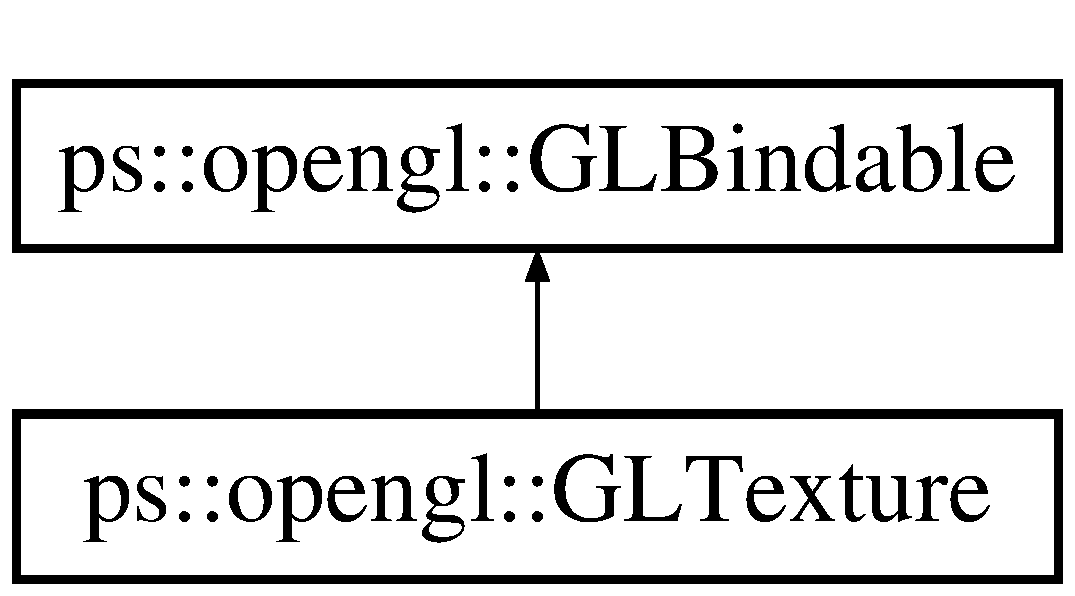
\includegraphics[height=2.000000cm]{classps_1_1opengl_1_1GLTexture}
\end{center}
\end{figure}
\subsection*{Public Types}
\begin{DoxyCompactItemize}
\item 
\hypertarget{classps_1_1opengl_1_1GLTexture_ac711ed7b8ea94b66349dd3f18af2abc0}{}enum {\bfseries Image\+File\+Type} \{ {\bfseries ift\+P\+N\+G}, 
{\bfseries ift\+B\+M\+P}, 
{\bfseries ift\+J\+P\+G}, 
{\bfseries ift\+Unsupported}
 \}\label{classps_1_1opengl_1_1GLTexture_ac711ed7b8ea94b66349dd3f18af2abc0}

\end{DoxyCompactItemize}
\subsection*{Public Member Functions}
\begin{DoxyCompactItemize}
\item 
\hypertarget{classps_1_1opengl_1_1GLTexture_ae99378a645c82f379dcb22e6dd4fcafc}{}{\bfseries G\+L\+Texture} (const \hyperlink{classps_1_1base_1_1CAString}{Ansi\+Str} \&str\+F\+P, int texunit=0)\label{classps_1_1opengl_1_1GLTexture_ae99378a645c82f379dcb22e6dd4fcafc}

\item 
\hypertarget{classps_1_1opengl_1_1GLTexture_ac022d03096e4237655c343498bb42e7a}{}void {\bfseries cleanup} ()\label{classps_1_1opengl_1_1GLTexture_ac022d03096e4237655c343498bb42e7a}

\item 
\hypertarget{classps_1_1opengl_1_1GLTexture_ac4e7ca9c8f54f4d164ab4961b6792bdb}{}bool {\bfseries read} (const \hyperlink{classps_1_1base_1_1CAString}{Ansi\+Str} \&str\+F\+P)\label{classps_1_1opengl_1_1GLTexture_ac4e7ca9c8f54f4d164ab4961b6792bdb}

\item 
\hypertarget{classps_1_1opengl_1_1GLTexture_affe70af1b538192d985bb62a403ca847}{}bool {\bfseries write} (const \hyperlink{classps_1_1base_1_1CAString}{Ansi\+Str} \&str\+F\+P)\label{classps_1_1opengl_1_1GLTexture_affe70af1b538192d985bb62a403ca847}

\item 
\hypertarget{classps_1_1opengl_1_1GLTexture_a94945c201c3714d1cf55dec4e529f75c}{}void {\bfseries set} (const \hyperlink{classps_1_1base_1_1Vec3}{vec3i} \&dim, U32 handle, int texunit=0)\label{classps_1_1opengl_1_1GLTexture_a94945c201c3714d1cf55dec4e529f75c}

\item 
\hypertarget{classps_1_1opengl_1_1GLTexture_a130c88e04751028a2de07e670462ea09}{}void {\bfseries bind} ()\label{classps_1_1opengl_1_1GLTexture_a130c88e04751028a2de07e670462ea09}

\item 
\hypertarget{classps_1_1opengl_1_1GLTexture_a8ae1327db35ec7d4a6948b174f3318d3}{}void {\bfseries unbind} ()\label{classps_1_1opengl_1_1GLTexture_a8ae1327db35ec7d4a6948b174f3318d3}

\item 
\hypertarget{classps_1_1opengl_1_1GLTexture_a211f23b09fa14e454908afe4c81c79c5}{}\hyperlink{classps_1_1base_1_1Vec3}{vec3i} {\bfseries dim} () const \label{classps_1_1opengl_1_1GLTexture_a211f23b09fa14e454908afe4c81c79c5}

\item 
\hypertarget{classps_1_1opengl_1_1GLTexture_a441699385e9443f1d6eb6ed9677fddbb}{}U32 {\bfseries handle} () const \label{classps_1_1opengl_1_1GLTexture_a441699385e9443f1d6eb6ed9677fddbb}

\end{DoxyCompactItemize}
\subsection*{Static Public Member Functions}
\begin{DoxyCompactItemize}
\item 
\hypertarget{classps_1_1opengl_1_1GLTexture_acfdb5ccaaae35d7181f2e02ad2ce334f}{}static Image\+File\+Type {\bfseries Get\+File\+Type} (const \hyperlink{classps_1_1base_1_1CAString}{Ansi\+Str} \&str\+F\+P)\label{classps_1_1opengl_1_1GLTexture_acfdb5ccaaae35d7181f2e02ad2ce334f}

\item 
\hypertarget{classps_1_1opengl_1_1GLTexture_a1acd6723be6c74830c1f421c18fe7ef7}{}static \hyperlink{classps_1_1opengl_1_1GLTexture}{G\+L\+Texture} $\ast$ {\bfseries Checker\+Board} ()\label{classps_1_1opengl_1_1GLTexture_a1acd6723be6c74830c1f421c18fe7ef7}

\end{DoxyCompactItemize}
\subsection*{Protected Attributes}
\begin{DoxyCompactItemize}
\item 
\hypertarget{classps_1_1opengl_1_1GLTexture_a4f182a1756309ca8a54014c2af1dde48}{}int {\bfseries m\+\_\+texunit}\label{classps_1_1opengl_1_1GLTexture_a4f182a1756309ca8a54014c2af1dde48}

\item 
\hypertarget{classps_1_1opengl_1_1GLTexture_a906c159323b7f804f153ddc81484479c}{}U32 {\bfseries m\+\_\+gl\+Tex}\label{classps_1_1opengl_1_1GLTexture_a906c159323b7f804f153ddc81484479c}

\item 
\hypertarget{classps_1_1opengl_1_1GLTexture_a638777de5607b5f8d65d06a2a57eb1a4}{}\hyperlink{classps_1_1base_1_1Vec3}{vec3i} {\bfseries m\+\_\+dim}\label{classps_1_1opengl_1_1GLTexture_a638777de5607b5f8d65d06a2a57eb1a4}

\end{DoxyCompactItemize}


The documentation for this class was generated from the following files\+:\begin{DoxyCompactItemize}
\item 
/\+Users/pourya/\+Desktop/platform/repos/tetcutter/src/glbackend/gltexture.\+h\item 
/\+Users/pourya/\+Desktop/platform/repos/tetcutter/src/glbackend/gltexture.\+cpp\end{DoxyCompactItemize}

\hypertarget{classps_1_1elastic_1_1HandleCorrection}{}\section{ps\+:\+:elastic\+:\+:Handle\+Correction Class Reference}
\label{classps_1_1elastic_1_1HandleCorrection}\index{ps\+::elastic\+::\+Handle\+Correction@{ps\+::elastic\+::\+Handle\+Correction}}
\subsection*{Public Member Functions}
\begin{DoxyCompactItemize}
\item 
\hypertarget{classps_1_1elastic_1_1HandleCorrection_a14d349e73a240cda6e4b55865f2dad03}{}{\bfseries Handle\+Correction} (U32 key)\label{classps_1_1elastic_1_1HandleCorrection_a14d349e73a240cda6e4b55865f2dad03}

\item 
\hypertarget{classps_1_1elastic_1_1HandleCorrection_a878dfb77b6725fdf8d7beec4981d6bef}{}void {\bfseries correct\+Vec\+Value} (std\+::vector$<$ U32 $>$ \&\+\_\+vec)\label{classps_1_1elastic_1_1HandleCorrection_a878dfb77b6725fdf8d7beec4981d6bef}

\item 
\hypertarget{classps_1_1elastic_1_1HandleCorrection_a06cdcfa94df46eafd1e9834919b76679}{}void {\bfseries correct\+Value} (U32 \&rhs)\label{classps_1_1elastic_1_1HandleCorrection_a06cdcfa94df46eafd1e9834919b76679}

\end{DoxyCompactItemize}


The documentation for this class was generated from the following file\+:\begin{DoxyCompactItemize}
\item 
/\+Users/pourya/\+Desktop/platform/repos/tetcutter/src/elastic/volmeshentities.\+h\end{DoxyCompactItemize}

\hypertarget{classps_1_1elastic_1_1HandleCorrectionParallel}{}\section{ps\+:\+:elastic\+:\+:Handle\+Correction\+Parallel Class Reference}
\label{classps_1_1elastic_1_1HandleCorrectionParallel}\index{ps\+::elastic\+::\+Handle\+Correction\+Parallel@{ps\+::elastic\+::\+Handle\+Correction\+Parallel}}
\subsection*{Public Member Functions}
\begin{DoxyCompactItemize}
\item 
\hypertarget{classps_1_1elastic_1_1HandleCorrectionParallel_ad9def55626e14e06bf41e3e233f905e1}{}{\bfseries Handle\+Correction\+Parallel} (U32 key, vector$<$ vector$<$ U32 $>$ $>$ \&container)\label{classps_1_1elastic_1_1HandleCorrectionParallel_ad9def55626e14e06bf41e3e233f905e1}

\item 
\hypertarget{classps_1_1elastic_1_1HandleCorrectionParallel_a27dc726eb77a9b6f0b85fe1d68b3e7a5}{}void {\bfseries operator()} (const blocked\+\_\+range$<$ U32 $>$ \&range) const \label{classps_1_1elastic_1_1HandleCorrectionParallel_a27dc726eb77a9b6f0b85fe1d68b3e7a5}

\end{DoxyCompactItemize}


The documentation for this class was generated from the following file\+:\begin{DoxyCompactItemize}
\item 
/\+Users/pourya/\+Desktop/platform/repos/tetcutter/src/elastic/volmeshentities.\+h\end{DoxyCompactItemize}

\hypertarget{classps_1_1PRIVATE_1_1holder}{}\section{ps\+:\+:P\+R\+I\+V\+A\+T\+E\+:\+:holder$<$ value\+\_\+type $>$ Class Template Reference}
\label{classps_1_1PRIVATE_1_1holder}\index{ps\+::\+P\+R\+I\+V\+A\+T\+E\+::holder$<$ value\+\_\+type $>$@{ps\+::\+P\+R\+I\+V\+A\+T\+E\+::holder$<$ value\+\_\+type $>$}}
Inheritance diagram for ps\+:\+:P\+R\+I\+V\+A\+T\+E\+:\+:holder$<$ value\+\_\+type $>$\+:\begin{figure}[H]
\begin{center}
\leavevmode
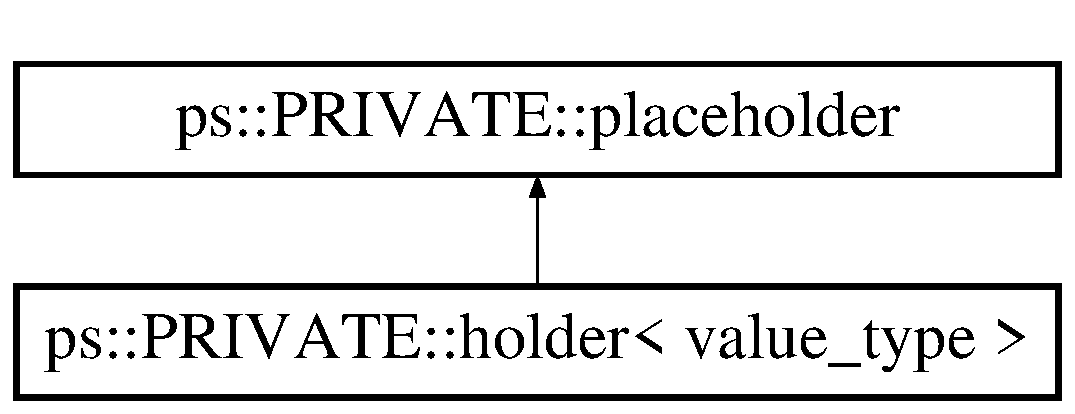
\includegraphics[height=2.000000cm]{classps_1_1PRIVATE_1_1holder}
\end{center}
\end{figure}
\subsection*{Public Member Functions}
\begin{DoxyCompactItemize}
\item 
\hypertarget{classps_1_1PRIVATE_1_1holder_a6ec3b7ccb33bad56c2181e0f68fa720b}{}{\bfseries holder} (const value\+\_\+type \&v)\label{classps_1_1PRIVATE_1_1holder_a6ec3b7ccb33bad56c2181e0f68fa720b}

\item 
\hypertarget{classps_1_1PRIVATE_1_1holder_a009fc3160cc8b3fd33e0b191632132b0}{}virtual const std\+::type\+\_\+info \& {\bfseries type\+\_\+info} () const \label{classps_1_1PRIVATE_1_1holder_a009fc3160cc8b3fd33e0b191632132b0}

\item 
\hypertarget{classps_1_1PRIVATE_1_1holder_a65ecbdebbf333cb8bf5c57f2b05a040d}{}virtual std\+::string {\bfseries to\+String} () const \label{classps_1_1PRIVATE_1_1holder_a65ecbdebbf333cb8bf5c57f2b05a040d}

\item 
\hypertarget{classps_1_1PRIVATE_1_1holder_a7695cacb686b48d794ebb9f3c80868f1}{}virtual void {\bfseries from\+String} (const string \&s)\label{classps_1_1PRIVATE_1_1holder_a7695cacb686b48d794ebb9f3c80868f1}

\item 
\hypertarget{classps_1_1PRIVATE_1_1holder_a2b3d976f5ea886f716c6cc529a420f0e}{}virtual \hyperlink{classps_1_1PRIVATE_1_1placeholder}{placeholder} $\ast$ {\bfseries clone} () const \label{classps_1_1PRIVATE_1_1holder_a2b3d976f5ea886f716c6cc529a420f0e}

\end{DoxyCompactItemize}
\subsection*{Public Attributes}
\begin{DoxyCompactItemize}
\item 
\hypertarget{classps_1_1PRIVATE_1_1holder_a51697997f55281b74d08b4f5b5e72553}{}value\+\_\+type {\bfseries held}\label{classps_1_1PRIVATE_1_1holder_a51697997f55281b74d08b4f5b5e72553}

\end{DoxyCompactItemize}


The documentation for this class was generated from the following file\+:\begin{DoxyCompactItemize}
\item 
/\+Users/pourya/\+Desktop/platform/repos/tetcutter/src/base/value.\+h\end{DoxyCompactItemize}

\hypertarget{classps_1_1PRIVATE_1_1holder_3_01AnsiStr_01_4}{}\section{ps\+:\+:P\+R\+I\+V\+A\+T\+E\+:\+:holder$<$ Ansi\+Str $>$ Class Template Reference}
\label{classps_1_1PRIVATE_1_1holder_3_01AnsiStr_01_4}\index{ps\+::\+P\+R\+I\+V\+A\+T\+E\+::holder$<$ Ansi\+Str $>$@{ps\+::\+P\+R\+I\+V\+A\+T\+E\+::holder$<$ Ansi\+Str $>$}}
Inheritance diagram for ps\+:\+:P\+R\+I\+V\+A\+T\+E\+:\+:holder$<$ Ansi\+Str $>$\+:\begin{figure}[H]
\begin{center}
\leavevmode
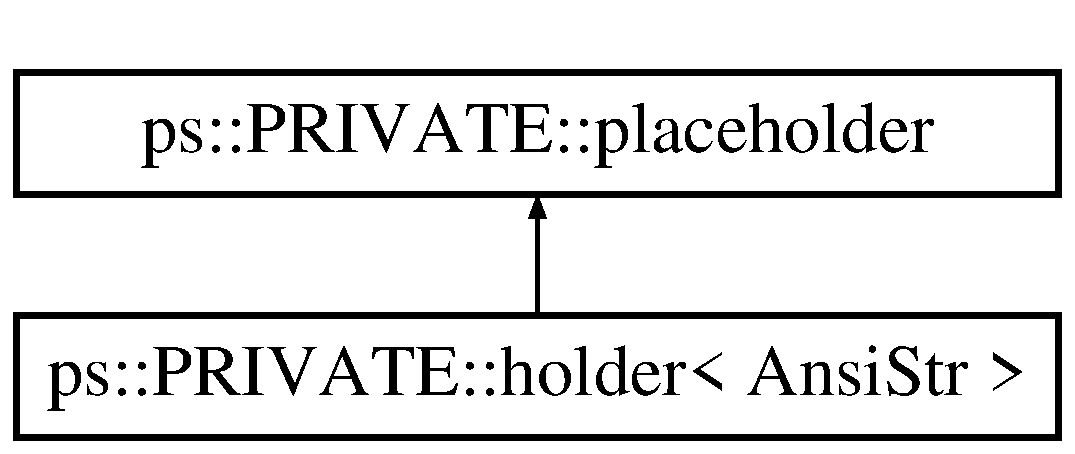
\includegraphics[height=2.000000cm]{classps_1_1PRIVATE_1_1holder_3_01AnsiStr_01_4}
\end{center}
\end{figure}
\subsection*{Public Member Functions}
\begin{DoxyCompactItemize}
\item 
\hypertarget{classps_1_1PRIVATE_1_1holder_3_01AnsiStr_01_4_af5d43f1b7b14dd48b7d5b6f8cd1bcc14}{}{\bfseries holder} (const \hyperlink{classps_1_1base_1_1CAString}{Ansi\+Str} \&str)\label{classps_1_1PRIVATE_1_1holder_3_01AnsiStr_01_4_af5d43f1b7b14dd48b7d5b6f8cd1bcc14}

\item 
\hypertarget{classps_1_1PRIVATE_1_1holder_3_01AnsiStr_01_4_abde716286bf24b45317e3a36ec52a200}{}std\+::string {\bfseries to\+String} () const \label{classps_1_1PRIVATE_1_1holder_3_01AnsiStr_01_4_abde716286bf24b45317e3a36ec52a200}

\item 
\hypertarget{classps_1_1PRIVATE_1_1holder_3_01AnsiStr_01_4_a55316f448722b9c9a0db5d686d9ecc91}{}void {\bfseries from\+String} (const string \&s)\label{classps_1_1PRIVATE_1_1holder_3_01AnsiStr_01_4_a55316f448722b9c9a0db5d686d9ecc91}

\item 
\hypertarget{classps_1_1PRIVATE_1_1holder_3_01AnsiStr_01_4_a46d3a8950ba041f9f62d6a9424bea07d}{}const std\+::type\+\_\+info \& {\bfseries type\+\_\+info} () const \label{classps_1_1PRIVATE_1_1holder_3_01AnsiStr_01_4_a46d3a8950ba041f9f62d6a9424bea07d}

\item 
\hypertarget{classps_1_1PRIVATE_1_1holder_3_01AnsiStr_01_4_a8344041badd357e3b79e071a993a8d6a}{}\hyperlink{classps_1_1PRIVATE_1_1placeholder}{placeholder} $\ast$ {\bfseries clone} () const \label{classps_1_1PRIVATE_1_1holder_3_01AnsiStr_01_4_a8344041badd357e3b79e071a993a8d6a}

\end{DoxyCompactItemize}
\subsection*{Public Attributes}
\begin{DoxyCompactItemize}
\item 
\hypertarget{classps_1_1PRIVATE_1_1holder_3_01AnsiStr_01_4_aa62f904f20189ed4f82c5ed4481272b3}{}\hyperlink{classps_1_1base_1_1CAString}{Ansi\+Str} {\bfseries held}\label{classps_1_1PRIVATE_1_1holder_3_01AnsiStr_01_4_aa62f904f20189ed4f82c5ed4481272b3}

\end{DoxyCompactItemize}


The documentation for this class was generated from the following file\+:\begin{DoxyCompactItemize}
\item 
/\+Users/pourya/\+Desktop/platform/repos/tetcutter/src/base/value.\+h\end{DoxyCompactItemize}

\hypertarget{classps_1_1PRIVATE_1_1holder_3_01vec2f_01_4}{}\section{ps\+:\+:P\+R\+I\+V\+A\+T\+E\+:\+:holder$<$ vec2f $>$ Class Template Reference}
\label{classps_1_1PRIVATE_1_1holder_3_01vec2f_01_4}\index{ps\+::\+P\+R\+I\+V\+A\+T\+E\+::holder$<$ vec2f $>$@{ps\+::\+P\+R\+I\+V\+A\+T\+E\+::holder$<$ vec2f $>$}}
Inheritance diagram for ps\+:\+:P\+R\+I\+V\+A\+T\+E\+:\+:holder$<$ vec2f $>$\+:\begin{figure}[H]
\begin{center}
\leavevmode
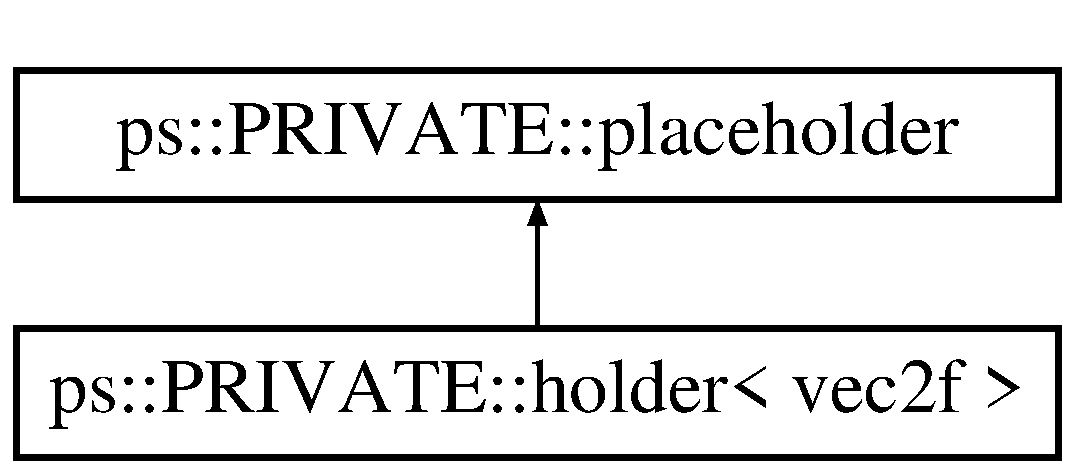
\includegraphics[height=2.000000cm]{classps_1_1PRIVATE_1_1holder_3_01vec2f_01_4}
\end{center}
\end{figure}
\subsection*{Public Member Functions}
\begin{DoxyCompactItemize}
\item 
\hypertarget{classps_1_1PRIVATE_1_1holder_3_01vec2f_01_4_a6738d9adcd60ced6543e16019dadf749}{}{\bfseries holder} (const \hyperlink{classps_1_1base_1_1Vec2}{vec2f} \&v)\label{classps_1_1PRIVATE_1_1holder_3_01vec2f_01_4_a6738d9adcd60ced6543e16019dadf749}

\item 
\hypertarget{classps_1_1PRIVATE_1_1holder_3_01vec2f_01_4_a0eeba4bcd65b6867eec4eafcb4712d45}{}std\+::string {\bfseries to\+String} () const \label{classps_1_1PRIVATE_1_1holder_3_01vec2f_01_4_a0eeba4bcd65b6867eec4eafcb4712d45}

\item 
\hypertarget{classps_1_1PRIVATE_1_1holder_3_01vec2f_01_4_aef8835c0de6f35a130aa8f50c67d64b0}{}void {\bfseries from\+String} (const string \&s)\label{classps_1_1PRIVATE_1_1holder_3_01vec2f_01_4_aef8835c0de6f35a130aa8f50c67d64b0}

\item 
\hypertarget{classps_1_1PRIVATE_1_1holder_3_01vec2f_01_4_a172a09ffff2fbcb45f22b08396f65bb3}{}const std\+::type\+\_\+info \& {\bfseries type\+\_\+info} () const \label{classps_1_1PRIVATE_1_1holder_3_01vec2f_01_4_a172a09ffff2fbcb45f22b08396f65bb3}

\item 
\hypertarget{classps_1_1PRIVATE_1_1holder_3_01vec2f_01_4_a06db4ced260049445e61d5b19b3491ef}{}\hyperlink{classps_1_1PRIVATE_1_1placeholder}{placeholder} $\ast$ {\bfseries clone} () const \label{classps_1_1PRIVATE_1_1holder_3_01vec2f_01_4_a06db4ced260049445e61d5b19b3491ef}

\end{DoxyCompactItemize}
\subsection*{Public Attributes}
\begin{DoxyCompactItemize}
\item 
\hypertarget{classps_1_1PRIVATE_1_1holder_3_01vec2f_01_4_a5d1a9e434bd8449f103cbb97713306aa}{}\hyperlink{classps_1_1base_1_1Vec2}{vec2f} {\bfseries held}\label{classps_1_1PRIVATE_1_1holder_3_01vec2f_01_4_a5d1a9e434bd8449f103cbb97713306aa}

\end{DoxyCompactItemize}


The documentation for this class was generated from the following file\+:\begin{DoxyCompactItemize}
\item 
/\+Users/pourya/\+Desktop/platform/repos/tetcutter/src/base/value.\+h\end{DoxyCompactItemize}

\hypertarget{classps_1_1PRIVATE_1_1holder_3_01vec3f_01_4}{}\section{ps\+:\+:P\+R\+I\+V\+A\+T\+E\+:\+:holder$<$ vec3f $>$ Class Template Reference}
\label{classps_1_1PRIVATE_1_1holder_3_01vec3f_01_4}\index{ps\+::\+P\+R\+I\+V\+A\+T\+E\+::holder$<$ vec3f $>$@{ps\+::\+P\+R\+I\+V\+A\+T\+E\+::holder$<$ vec3f $>$}}
Inheritance diagram for ps\+:\+:P\+R\+I\+V\+A\+T\+E\+:\+:holder$<$ vec3f $>$\+:\begin{figure}[H]
\begin{center}
\leavevmode
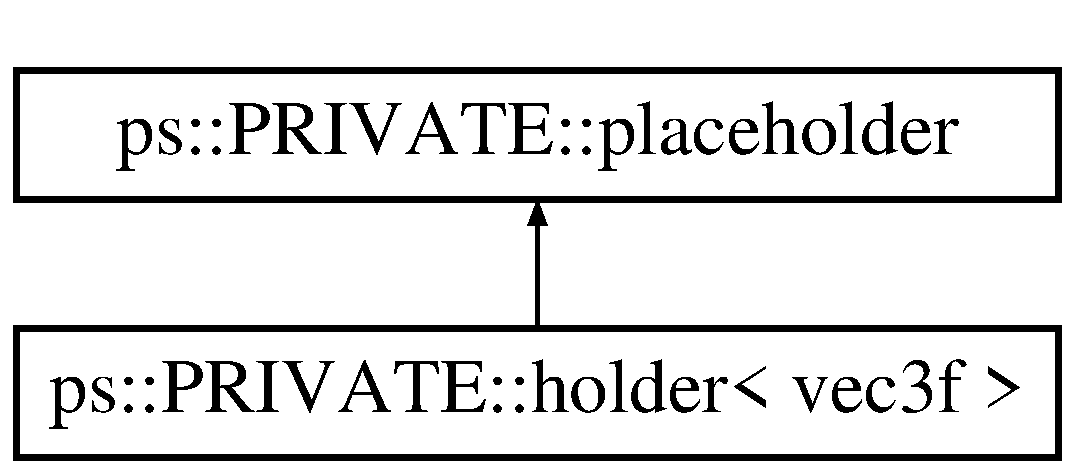
\includegraphics[height=2.000000cm]{classps_1_1PRIVATE_1_1holder_3_01vec3f_01_4}
\end{center}
\end{figure}
\subsection*{Public Member Functions}
\begin{DoxyCompactItemize}
\item 
\hypertarget{classps_1_1PRIVATE_1_1holder_3_01vec3f_01_4_acffc22ac5f431948ae1e8bf629a6bb3f}{}{\bfseries holder} (const \hyperlink{classps_1_1base_1_1Vec3}{vec3f} \&v)\label{classps_1_1PRIVATE_1_1holder_3_01vec3f_01_4_acffc22ac5f431948ae1e8bf629a6bb3f}

\item 
\hypertarget{classps_1_1PRIVATE_1_1holder_3_01vec3f_01_4_a5ce11e3198303498c46ca6974b935434}{}std\+::string {\bfseries to\+String} () const \label{classps_1_1PRIVATE_1_1holder_3_01vec3f_01_4_a5ce11e3198303498c46ca6974b935434}

\item 
\hypertarget{classps_1_1PRIVATE_1_1holder_3_01vec3f_01_4_a567e3ed7dff33e829ef2b306d8f44eb7}{}void {\bfseries from\+String} (const string \&s)\label{classps_1_1PRIVATE_1_1holder_3_01vec3f_01_4_a567e3ed7dff33e829ef2b306d8f44eb7}

\item 
\hypertarget{classps_1_1PRIVATE_1_1holder_3_01vec3f_01_4_a7f3948aacc1eb0faa52936545f38107b}{}const std\+::type\+\_\+info \& {\bfseries type\+\_\+info} () const \label{classps_1_1PRIVATE_1_1holder_3_01vec3f_01_4_a7f3948aacc1eb0faa52936545f38107b}

\item 
\hypertarget{classps_1_1PRIVATE_1_1holder_3_01vec3f_01_4_aa80087c995c80c03ef9e3d61c1f0cd6b}{}\hyperlink{classps_1_1PRIVATE_1_1placeholder}{placeholder} $\ast$ {\bfseries clone} () const \label{classps_1_1PRIVATE_1_1holder_3_01vec3f_01_4_aa80087c995c80c03ef9e3d61c1f0cd6b}

\end{DoxyCompactItemize}
\subsection*{Public Attributes}
\begin{DoxyCompactItemize}
\item 
\hypertarget{classps_1_1PRIVATE_1_1holder_3_01vec3f_01_4_a315bc8fcab0df0aff5d8a87e1c5c710c}{}\hyperlink{classps_1_1base_1_1Vec3}{vec3f} {\bfseries held}\label{classps_1_1PRIVATE_1_1holder_3_01vec3f_01_4_a315bc8fcab0df0aff5d8a87e1c5c710c}

\end{DoxyCompactItemize}


The documentation for this class was generated from the following file\+:\begin{DoxyCompactItemize}
\item 
/\+Users/pourya/\+Desktop/platform/repos/tetcutter/src/base/value.\+h\end{DoxyCompactItemize}

\hypertarget{classps_1_1PRIVATE_1_1holder_3_01vec4f_01_4}{}\section{ps\+:\+:P\+R\+I\+V\+A\+T\+E\+:\+:holder$<$ vec4f $>$ Class Template Reference}
\label{classps_1_1PRIVATE_1_1holder_3_01vec4f_01_4}\index{ps\+::\+P\+R\+I\+V\+A\+T\+E\+::holder$<$ vec4f $>$@{ps\+::\+P\+R\+I\+V\+A\+T\+E\+::holder$<$ vec4f $>$}}
Inheritance diagram for ps\+:\+:P\+R\+I\+V\+A\+T\+E\+:\+:holder$<$ vec4f $>$\+:\begin{figure}[H]
\begin{center}
\leavevmode
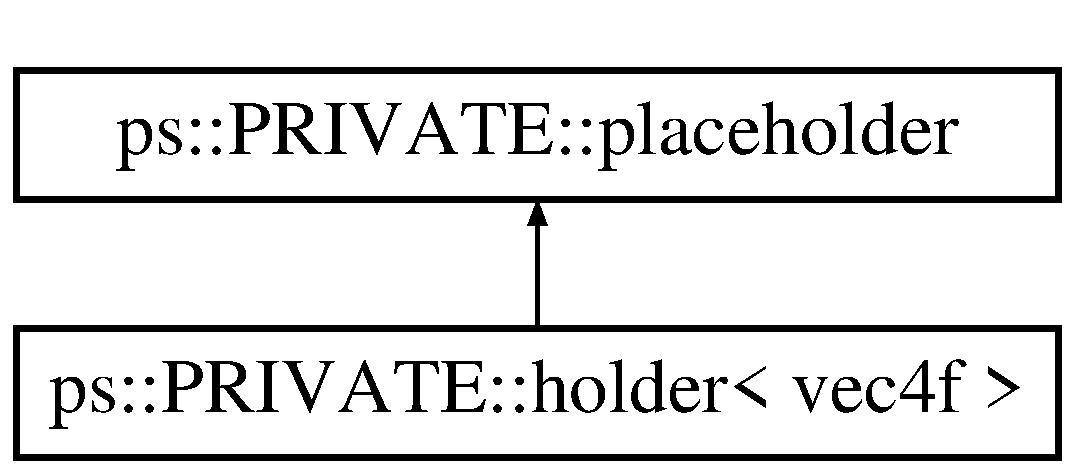
\includegraphics[height=2.000000cm]{classps_1_1PRIVATE_1_1holder_3_01vec4f_01_4}
\end{center}
\end{figure}
\subsection*{Public Member Functions}
\begin{DoxyCompactItemize}
\item 
\hypertarget{classps_1_1PRIVATE_1_1holder_3_01vec4f_01_4_aa064c4552601de818ab29094fce8c4b7}{}{\bfseries holder} (const \hyperlink{classps_1_1base_1_1Vec4}{vec4f} \&v)\label{classps_1_1PRIVATE_1_1holder_3_01vec4f_01_4_aa064c4552601de818ab29094fce8c4b7}

\item 
\hypertarget{classps_1_1PRIVATE_1_1holder_3_01vec4f_01_4_a257b7630a6a46f725999e578f599413f}{}std\+::string {\bfseries to\+String} () const \label{classps_1_1PRIVATE_1_1holder_3_01vec4f_01_4_a257b7630a6a46f725999e578f599413f}

\item 
\hypertarget{classps_1_1PRIVATE_1_1holder_3_01vec4f_01_4_a245b964ae8bbb1347a3876dad358d36a}{}void {\bfseries from\+String} (const string \&s)\label{classps_1_1PRIVATE_1_1holder_3_01vec4f_01_4_a245b964ae8bbb1347a3876dad358d36a}

\item 
\hypertarget{classps_1_1PRIVATE_1_1holder_3_01vec4f_01_4_ae5ec0c1907a61cbce5a62b99fd702902}{}const std\+::type\+\_\+info \& {\bfseries type\+\_\+info} () const \label{classps_1_1PRIVATE_1_1holder_3_01vec4f_01_4_ae5ec0c1907a61cbce5a62b99fd702902}

\item 
\hypertarget{classps_1_1PRIVATE_1_1holder_3_01vec4f_01_4_ad5590c2522fa26294998e4b4593a279d}{}\hyperlink{classps_1_1PRIVATE_1_1placeholder}{placeholder} $\ast$ {\bfseries clone} () const \label{classps_1_1PRIVATE_1_1holder_3_01vec4f_01_4_ad5590c2522fa26294998e4b4593a279d}

\end{DoxyCompactItemize}
\subsection*{Public Attributes}
\begin{DoxyCompactItemize}
\item 
\hypertarget{classps_1_1PRIVATE_1_1holder_3_01vec4f_01_4_ab7c277fc6ca38db0a67f2d786aad6a3e}{}\hyperlink{classps_1_1base_1_1Vec4}{vec4f} {\bfseries held}\label{classps_1_1PRIVATE_1_1holder_3_01vec4f_01_4_ab7c277fc6ca38db0a67f2d786aad6a3e}

\end{DoxyCompactItemize}


The documentation for this class was generated from the following file\+:\begin{DoxyCompactItemize}
\item 
/\+Users/pourya/\+Desktop/platform/repos/tetcutter/src/base/value.\+h\end{DoxyCompactItemize}

\hypertarget{classps_1_1elastic_1_1IAvatar}{}\section{ps\+:\+:elastic\+:\+:I\+Avatar Class Reference}
\label{classps_1_1elastic_1_1IAvatar}\index{ps\+::elastic\+::\+I\+Avatar@{ps\+::elastic\+::\+I\+Avatar}}
Inheritance diagram for ps\+:\+:elastic\+:\+:I\+Avatar\+:\begin{figure}[H]
\begin{center}
\leavevmode
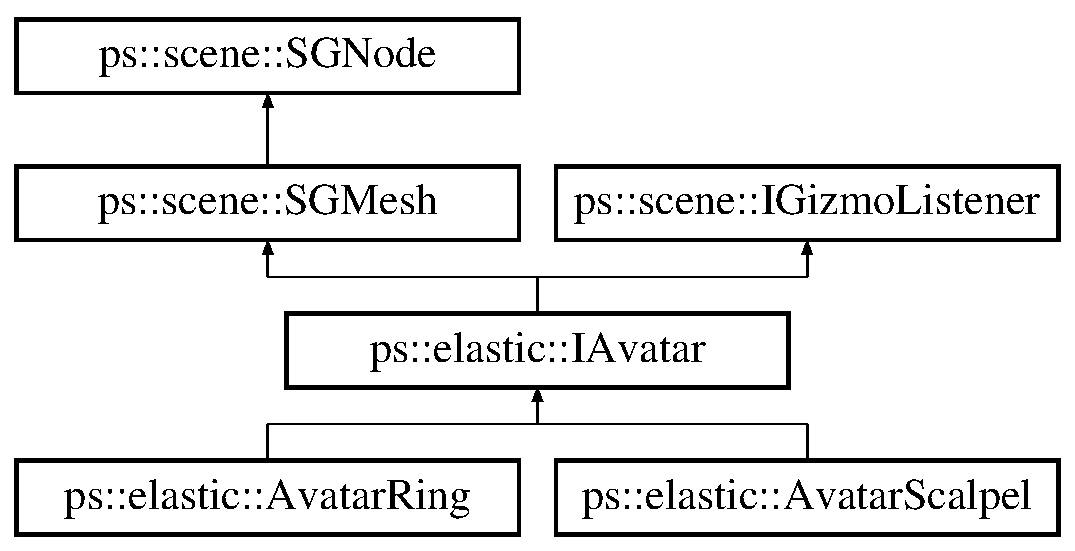
\includegraphics[height=4.000000cm]{classps_1_1elastic_1_1IAvatar}
\end{center}
\end{figure}
\subsection*{Public Types}
\begin{DoxyCompactItemize}
\item 
\hypertarget{classps_1_1elastic_1_1IAvatar_a3fe07bb0b1d429a8e80c893b997bdbe5}{}typedef std\+::function$<$ void()$>$ {\bfseries On\+Cut\+Finished}\label{classps_1_1elastic_1_1IAvatar_a3fe07bb0b1d429a8e80c893b997bdbe5}

\end{DoxyCompactItemize}
\subsection*{Public Member Functions}
\begin{DoxyCompactItemize}
\item 
\hypertarget{classps_1_1elastic_1_1IAvatar_a4d83a218b91fd1723c519c853ffbe7e6}{}{\bfseries I\+Avatar} (\hyperlink{classps_1_1elastic_1_1CuttableMesh}{Cuttable\+Mesh} $\ast$pmesh)\label{classps_1_1elastic_1_1IAvatar_a4d83a218b91fd1723c519c853ffbe7e6}

\item 
\hypertarget{classps_1_1elastic_1_1IAvatar_aa50d23f7f090f5c632c5b86a78c9d459}{}virtual void {\bfseries clear\+Cut\+Context} ()\label{classps_1_1elastic_1_1IAvatar_aa50d23f7f090f5c632c5b86a78c9d459}

\item 
\hypertarget{classps_1_1elastic_1_1IAvatar_a4a4baa68f08633a045b026970528b11a}{}void {\bfseries set\+On\+Cut\+Finished\+Event\+Handler} (On\+Cut\+Finished f)\label{classps_1_1elastic_1_1IAvatar_a4a4baa68f08633a045b026970528b11a}

\item 
\hypertarget{classps_1_1elastic_1_1IAvatar_ab841e482707e9d66e60c5b006a2b42c6}{}void {\bfseries set\+Tissue} (\hyperlink{classps_1_1elastic_1_1CuttableMesh}{Cuttable\+Mesh} $\ast$tissue)\label{classps_1_1elastic_1_1IAvatar_ab841e482707e9d66e60c5b006a2b42c6}

\item 
\hypertarget{classps_1_1elastic_1_1IAvatar_a6baf340b02f3505259d3e6ad70407347}{}virtual void {\bfseries grip} ()\label{classps_1_1elastic_1_1IAvatar_a6baf340b02f3505259d3e6ad70407347}

\item 
\hypertarget{classps_1_1elastic_1_1IAvatar_a44b53d02a1416efe7d9d9ec4f7b343d3}{}bool {\bfseries is\+Grip\+Active} () const \label{classps_1_1elastic_1_1IAvatar_a44b53d02a1416efe7d9d9ec4f7b343d3}

\item 
\hypertarget{classps_1_1elastic_1_1IAvatar_a6e78ef39d5dcc024a32cecbbcefb7d75}{}bool {\bfseries is\+Active} () const \label{classps_1_1elastic_1_1IAvatar_a6e78ef39d5dcc024a32cecbbcefb7d75}

\item 
\hypertarget{classps_1_1elastic_1_1IAvatar_a3613c7eaae173b24dae94b7ff461d773}{}void {\bfseries update\+Vol\+Mesh\+Info\+Header} () const \label{classps_1_1elastic_1_1IAvatar_a3613c7eaae173b24dae94b7ff461d773}

\item 
\hypertarget{classps_1_1elastic_1_1IAvatar_a1591eb04ef1027916f5c4d14c2d23d2e}{}virtual void {\bfseries on\+Start} () override\label{classps_1_1elastic_1_1IAvatar_a1591eb04ef1027916f5c4d14c2d23d2e}

\item 
\hypertarget{classps_1_1elastic_1_1IAvatar_ae4e4ce7bd3e980be0d8aeef5e9d1c6be}{}virtual void {\bfseries on\+Stop} () override\label{classps_1_1elastic_1_1IAvatar_ae4e4ce7bd3e980be0d8aeef5e9d1c6be}

\item 
\hypertarget{classps_1_1elastic_1_1IAvatar_a5493dfe996c2a72c6f623214a4296887}{}virtual void {\bfseries on\+Reset} () override\label{classps_1_1elastic_1_1IAvatar_a5493dfe996c2a72c6f623214a4296887}

\end{DoxyCompactItemize}
\subsection*{Protected Member Functions}
\begin{DoxyCompactItemize}
\item 
\hypertarget{classps_1_1elastic_1_1IAvatar_ac9d23b648ec205f7ad741d4f59bf72f5}{}void {\bfseries init} ()\label{classps_1_1elastic_1_1IAvatar_ac9d23b648ec205f7ad741d4f59bf72f5}

\end{DoxyCompactItemize}
\subsection*{Protected Attributes}
\begin{DoxyCompactItemize}
\item 
\hypertarget{classps_1_1elastic_1_1IAvatar_a43b7bc51b57ff45402b0b578cff62aa1}{}bool {\bfseries m\+\_\+is\+Tool\+Active}\label{classps_1_1elastic_1_1IAvatar_a43b7bc51b57ff45402b0b578cff62aa1}

\item 
\hypertarget{classps_1_1elastic_1_1IAvatar_a646c4b11d23e36ec4d37164e584a6b2c}{}bool {\bfseries m\+\_\+apply\+Gripper}\label{classps_1_1elastic_1_1IAvatar_a646c4b11d23e36ec4d37164e584a6b2c}

\item 
\hypertarget{classps_1_1elastic_1_1IAvatar_a3a1e8ca01e6c15ad5e7d72f408587361}{}On\+Cut\+Finished {\bfseries m\+\_\+f\+On\+Cut\+Finished}\label{classps_1_1elastic_1_1IAvatar_a3a1e8ca01e6c15ad5e7d72f408587361}

\item 
\hypertarget{classps_1_1elastic_1_1IAvatar_aa366076ebb230205c1c068539cde0e4a}{}\hyperlink{classps_1_1elastic_1_1CuttableMesh}{Cuttable\+Mesh} $\ast$ {\bfseries m\+\_\+lp\+Tissue}\label{classps_1_1elastic_1_1IAvatar_aa366076ebb230205c1c068539cde0e4a}

\end{DoxyCompactItemize}


The documentation for this class was generated from the following files\+:\begin{DoxyCompactItemize}
\item 
/\+Users/pourya/\+Desktop/platform/repos/tetcutter/src/elastic/iavatar.\+h\item 
/\+Users/pourya/\+Desktop/platform/repos/tetcutter/src/elastic/iavatar.\+cpp\end{DoxyCompactItemize}

\hypertarget{classps_1_1scene_1_1IGizmoListener}{}\section{ps\+:\+:scene\+:\+:I\+Gizmo\+Listener Class Reference}
\label{classps_1_1scene_1_1IGizmoListener}\index{ps\+::scene\+::\+I\+Gizmo\+Listener@{ps\+::scene\+::\+I\+Gizmo\+Listener}}
Inheritance diagram for ps\+:\+:scene\+:\+:I\+Gizmo\+Listener\+:\begin{figure}[H]
\begin{center}
\leavevmode
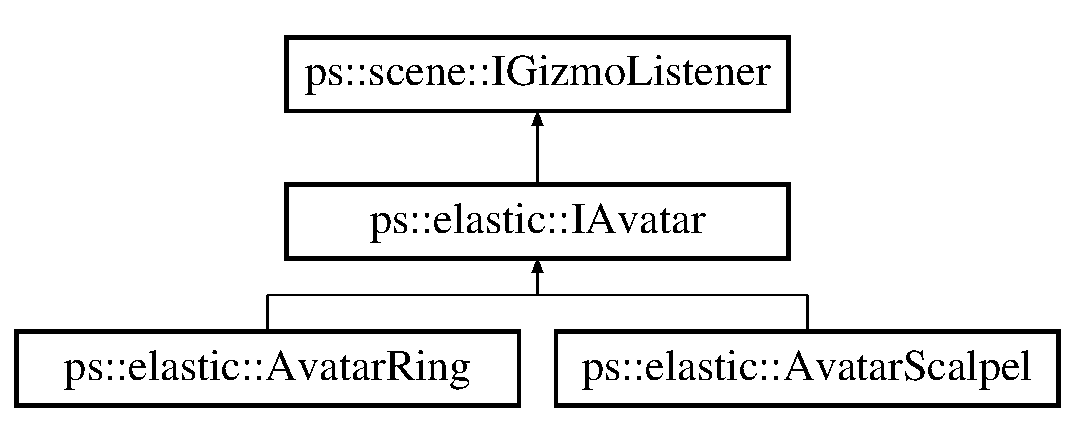
\includegraphics[height=3.000000cm]{classps_1_1scene_1_1IGizmoListener}
\end{center}
\end{figure}
\subsection*{Public Member Functions}
\begin{DoxyCompactItemize}
\item 
\hypertarget{classps_1_1scene_1_1IGizmoListener_a886e9f5f71c6800e4a5444accde10800}{}virtual void {\bfseries on\+Translate} (const \hyperlink{classps_1_1base_1_1Vec3}{vec3f} \&delta, const \hyperlink{classps_1_1base_1_1Vec3}{vec3f} \&pos)\label{classps_1_1scene_1_1IGizmoListener_a886e9f5f71c6800e4a5444accde10800}

\item 
\hypertarget{classps_1_1scene_1_1IGizmoListener_a11627a28e5e3cb1638cd1750cc9b3ea8}{}virtual void {\bfseries on\+Scale} (const \hyperlink{classps_1_1base_1_1Vec3}{vec3f} \&delta, const \hyperlink{classps_1_1base_1_1Vec3}{vec3f} \&current)\label{classps_1_1scene_1_1IGizmoListener_a11627a28e5e3cb1638cd1750cc9b3ea8}

\item 
\hypertarget{classps_1_1scene_1_1IGizmoListener_add8ff2601e9e6de1bf1aaf74ca36a51b}{}virtual void {\bfseries on\+Rotate} (const \hyperlink{classps_1_1base_1_1Quaternion}{quatf} \&delta)\label{classps_1_1scene_1_1IGizmoListener_add8ff2601e9e6de1bf1aaf74ca36a51b}

\item 
\hypertarget{classps_1_1scene_1_1IGizmoListener_ac1c3aa8fc797dea67a43286da7d4700b}{}virtual void {\bfseries on\+Start} ()\label{classps_1_1scene_1_1IGizmoListener_ac1c3aa8fc797dea67a43286da7d4700b}

\item 
\hypertarget{classps_1_1scene_1_1IGizmoListener_acd70fca1111038529305917dbfea5241}{}virtual void {\bfseries on\+Stop} ()\label{classps_1_1scene_1_1IGizmoListener_acd70fca1111038529305917dbfea5241}

\item 
\hypertarget{classps_1_1scene_1_1IGizmoListener_a81d14144400675c14bad117e91996bfb}{}virtual void {\bfseries on\+Reset} ()\label{classps_1_1scene_1_1IGizmoListener_a81d14144400675c14bad117e91996bfb}

\item 
\hypertarget{classps_1_1scene_1_1IGizmoListener_aa98fca5599db5a0c89abb3642c96671b}{}bool {\bfseries register\+Listener} ()\label{classps_1_1scene_1_1IGizmoListener_aa98fca5599db5a0c89abb3642c96671b}

\item 
\hypertarget{classps_1_1scene_1_1IGizmoListener_aca08d588bfacbac0cf3ed8c4023ef93f}{}void {\bfseries unregister\+Listener} ()\label{classps_1_1scene_1_1IGizmoListener_aca08d588bfacbac0cf3ed8c4023ef93f}

\end{DoxyCompactItemize}
\subsection*{Protected Attributes}
\begin{DoxyCompactItemize}
\item 
\hypertarget{classps_1_1scene_1_1IGizmoListener_af10f71e40619e8b82a6057616d0effdd}{}int {\bfseries m\+\_\+id}\label{classps_1_1scene_1_1IGizmoListener_af10f71e40619e8b82a6057616d0effdd}

\end{DoxyCompactItemize}


The documentation for this class was generated from the following files\+:\begin{DoxyCompactItemize}
\item 
/\+Users/pourya/\+Desktop/platform/repos/tetcutter/src/scene/gizmo.\+h\item 
/\+Users/pourya/\+Desktop/platform/repos/tetcutter/src/scene/gizmo.\+cpp\end{DoxyCompactItemize}

\hypertarget{classps_1_1IMouseListener}{}\section{ps\+:\+:I\+Mouse\+Listener Class Reference}
\label{classps_1_1IMouseListener}\index{ps\+::\+I\+Mouse\+Listener@{ps\+::\+I\+Mouse\+Listener}}
Inheritance diagram for ps\+:\+:I\+Mouse\+Listener\+:\begin{figure}[H]
\begin{center}
\leavevmode
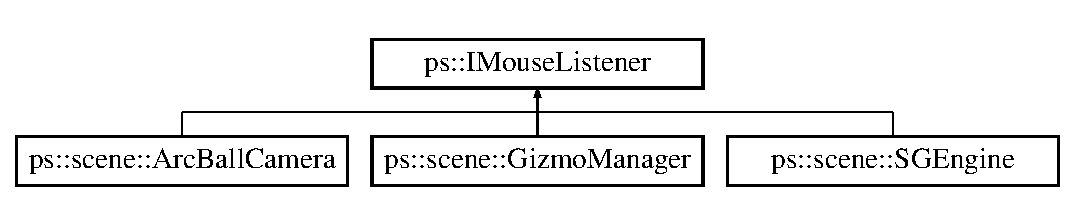
\includegraphics[height=2.000000cm]{classps_1_1IMouseListener}
\end{center}
\end{figure}
\subsection*{Public Member Functions}
\begin{DoxyCompactItemize}
\item 
\hypertarget{classps_1_1IMouseListener_ac30b7cd36737a4872b14a6dcbfaa88a7}{}virtual void {\bfseries mouse\+Press} (Mouse\+Button button, Mouse\+Button\+State state, int x, int y)=0\label{classps_1_1IMouseListener_ac30b7cd36737a4872b14a6dcbfaa88a7}

\item 
\hypertarget{classps_1_1IMouseListener_a1367f4f01d79dbc53d2093ac77008ca2}{}virtual void {\bfseries mouse\+Wheel} (Mouse\+Wheel\+Dir dir)=0\label{classps_1_1IMouseListener_a1367f4f01d79dbc53d2093ac77008ca2}

\item 
\hypertarget{classps_1_1IMouseListener_a7e36ab6e79d160fe32149a5334e74635}{}virtual void {\bfseries mouse\+Move} (int x, int y)=0\label{classps_1_1IMouseListener_a7e36ab6e79d160fe32149a5334e74635}

\item 
\hypertarget{classps_1_1IMouseListener_a70483b82ea66860b5d51303c63af9dda}{}bool {\bfseries focus} () const \label{classps_1_1IMouseListener_a70483b82ea66860b5d51303c63af9dda}

\item 
\hypertarget{classps_1_1IMouseListener_a430f1e62d5072a0177715135d6640d99}{}void {\bfseries set\+Focus} (bool focus)\label{classps_1_1IMouseListener_a430f1e62d5072a0177715135d6640d99}

\end{DoxyCompactItemize}
\subsection*{Protected Attributes}
\begin{DoxyCompactItemize}
\item 
\hypertarget{classps_1_1IMouseListener_a94bdb76017ab7539c809c2c58b104971}{}bool {\bfseries m\+\_\+is\+Focused}\label{classps_1_1IMouseListener_a94bdb76017ab7539c809c2c58b104971}

\end{DoxyCompactItemize}


The documentation for this class was generated from the following files\+:\begin{DoxyCompactItemize}
\item 
/\+Users/pourya/\+Desktop/platform/repos/tetcutter/src/base/imouselistener.\+h\item 
/\+Users/pourya/\+Desktop/platform/repos/tetcutter/src/base/imouselistener.\+cpp\end{DoxyCompactItemize}

\hypertarget{classps_1_1utils_1_1IniFile}{}\section{ps\+:\+:utils\+:\+:Ini\+File Class Reference}
\label{classps_1_1utils_1_1IniFile}\index{ps\+::utils\+::\+Ini\+File@{ps\+::utils\+::\+Ini\+File}}
\subsection*{Public Types}
\begin{DoxyCompactItemize}
\item 
\hypertarget{classps_1_1utils_1_1IniFile_a80edfc4b159559e04445a5d9cedc2c1f}{}enum {\bfseries File\+Mode} \{ {\bfseries fm\+Read}, 
{\bfseries fm\+Write}, 
{\bfseries fm\+Read\+Write}, 
{\bfseries fm\+Memory\+Stream}
 \}\label{classps_1_1utils_1_1IniFile_a80edfc4b159559e04445a5d9cedc2c1f}

\end{DoxyCompactItemize}
\subsection*{Public Member Functions}
\begin{DoxyCompactItemize}
\item 
\hypertarget{classps_1_1utils_1_1IniFile_a33ce9f03f3f70c25e5d38ced09f481d2}{}{\bfseries Ini\+File} (const \hyperlink{classps_1_1base_1_1CAString}{Ansi\+Str} \&str\+File\+Name, File\+Mode mode=fm\+Read\+Write)\label{classps_1_1utils_1_1IniFile_a33ce9f03f3f70c25e5d38ced09f481d2}

\item 
\hypertarget{classps_1_1utils_1_1IniFile_aabe8563b7528ec69b2c09e853d888a3a}{}File\+Mode {\bfseries get\+File\+Mode} () const \label{classps_1_1utils_1_1IniFile_aabe8563b7528ec69b2c09e853d888a3a}

\item 
\hypertarget{classps_1_1utils_1_1IniFile_a8dc30778ae042ee0f6059d4e897c9598}{}\hyperlink{classps_1_1base_1_1CAString}{Ansi\+Str} {\bfseries get\+File\+Name} () const \label{classps_1_1utils_1_1IniFile_a8dc30778ae042ee0f6059d4e897c9598}

\item 
\hypertarget{classps_1_1utils_1_1IniFile_aa7cc97c94e5e961fe429fdc458edcdb5}{}int {\bfseries extract\+Section} (const \hyperlink{classps_1_1base_1_1CAString}{Ansi\+Str} \&title, std\+::vector$<$ \hyperlink{classps_1_1base_1_1CAString}{Ansi\+Str} $>$ \&lines)\label{classps_1_1utils_1_1IniFile_aa7cc97c94e5e961fe429fdc458edcdb5}

\item 
\hypertarget{classps_1_1utils_1_1IniFile_af3b90889481cbbc3499b959cd7eca0b5}{}void {\bfseries clear\+Content\+Buffer} ()\label{classps_1_1utils_1_1IniFile_af3b90889481cbbc3499b959cd7eca0b5}

\item 
\hypertarget{classps_1_1utils_1_1IniFile_a6ecd023595e6c6e44a46804aa557d4a0}{}void {\bfseries get\+Content\+Buffer} (std\+::vector$<$ \hyperlink{classps_1_1base_1_1CAString}{Ansi\+Str} $>$ out\+Content\+Buf) const \label{classps_1_1utils_1_1IniFile_a6ecd023595e6c6e44a46804aa557d4a0}

\item 
\hypertarget{classps_1_1utils_1_1IniFile_a62a5f4a75b1c45a0e5cd166fd43af646}{}void {\bfseries set\+Content\+Buffer} (const std\+::vector$<$ \hyperlink{classps_1_1base_1_1CAString}{Ansi\+Str} $>$ \&in\+Content\+Buf)\label{classps_1_1utils_1_1IniFile_a62a5f4a75b1c45a0e5cd166fd43af646}

\item 
\hypertarget{classps_1_1utils_1_1IniFile_ae8fb149fa22d610954c46ca66904b6a5}{}void {\bfseries set} (const \hyperlink{classps_1_1base_1_1CAString}{Ansi\+Str} \&str\+File\+Name, File\+Mode mode=fm\+Read\+Write)\label{classps_1_1utils_1_1IniFile_ae8fb149fa22d610954c46ca66904b6a5}

\item 
\hypertarget{classps_1_1utils_1_1IniFile_a8205bc39dae3c81eef8d8ecd6415c341}{}bool {\bfseries set\+For\+Read} ()\label{classps_1_1utils_1_1IniFile_a8205bc39dae3c81eef8d8ecd6415c341}

\item 
\hypertarget{classps_1_1utils_1_1IniFile_aa9878c7a066bbde67e7b7d81d9de1188}{}void {\bfseries set\+For\+Write} ()\label{classps_1_1utils_1_1IniFile_aa9878c7a066bbde67e7b7d81d9de1188}

\item 
\hypertarget{classps_1_1utils_1_1IniFile_a769059b86ee86ab853270f9b20c37662}{}\hyperlink{classps_1_1base_1_1CAString}{Ansi\+Str} {\bfseries get\+File\+Path} () const \label{classps_1_1utils_1_1IniFile_a769059b86ee86ab853270f9b20c37662}

\item 
\hypertarget{classps_1_1utils_1_1IniFile_a04e55cb072e34470192bd84112308778}{}int {\bfseries has\+Section} (const \hyperlink{classps_1_1base_1_1CAString}{Ansi\+Str} \&str\+Section)\label{classps_1_1utils_1_1IniFile_a04e55cb072e34470192bd84112308778}

\item 
\hypertarget{classps_1_1utils_1_1IniFile_ab4b96643273bbd43814514df6c3cb716}{}bool {\bfseries write\+Value} (const \hyperlink{classps_1_1base_1_1CAString}{Ansi\+Str} \&section, const \hyperlink{classps_1_1base_1_1CAString}{Ansi\+Str} \&variable, const \hyperlink{classps_1_1base_1_1CAString}{Ansi\+Str} \&str\+Value)\label{classps_1_1utils_1_1IniFile_ab4b96643273bbd43814514df6c3cb716}

\item 
\hypertarget{classps_1_1utils_1_1IniFile_ac1f7d9eeabf23affb0a596b332313aee}{}bool {\bfseries read\+Line} (const \hyperlink{classps_1_1base_1_1CAString}{Ansi\+Str} \&section, const \hyperlink{classps_1_1base_1_1CAString}{Ansi\+Str} \&variable, \hyperlink{classps_1_1base_1_1CAString}{Ansi\+Str} \&str\+Line)\label{classps_1_1utils_1_1IniFile_ac1f7d9eeabf23affb0a596b332313aee}

\item 
\hypertarget{classps_1_1utils_1_1IniFile_a6be2b512881ff9957daf3743a2801d86}{}bool {\bfseries read\+Value} (const \hyperlink{classps_1_1base_1_1CAString}{Ansi\+Str} \&section, const \hyperlink{classps_1_1base_1_1CAString}{Ansi\+Str} \&variable, \hyperlink{classps_1_1base_1_1CAString}{Ansi\+Str} \&str\+Value)\label{classps_1_1utils_1_1IniFile_a6be2b512881ff9957daf3743a2801d86}

\item 
\hypertarget{classps_1_1utils_1_1IniFile_a3eb09c6424b2f1d82fe7008445838fed}{}int {\bfseries read\+Int} (const \hyperlink{classps_1_1base_1_1CAString}{Ansi\+Str} \&section, const \hyperlink{classps_1_1base_1_1CAString}{Ansi\+Str} \&variable, int def=0)\label{classps_1_1utils_1_1IniFile_a3eb09c6424b2f1d82fe7008445838fed}

\item 
\hypertarget{classps_1_1utils_1_1IniFile_a0ebbcfb0c2053b526665893902dfbdc9}{}void {\bfseries write\+Int} (const \hyperlink{classps_1_1base_1_1CAString}{Ansi\+Str} \&section, const \hyperlink{classps_1_1base_1_1CAString}{Ansi\+Str} \&variable, int val)\label{classps_1_1utils_1_1IniFile_a0ebbcfb0c2053b526665893902dfbdc9}

\item 
\hypertarget{classps_1_1utils_1_1IniFile_a5d06bd9d2c705cf333fb9fc5af9f1e04}{}float {\bfseries read\+Float} (const \hyperlink{classps_1_1base_1_1CAString}{Ansi\+Str} \&section, const \hyperlink{classps_1_1base_1_1CAString}{Ansi\+Str} \&variable, float def=0.\+0f)\label{classps_1_1utils_1_1IniFile_a5d06bd9d2c705cf333fb9fc5af9f1e04}

\item 
\hypertarget{classps_1_1utils_1_1IniFile_a5eca8b88c79d70495281dde32a286eb4}{}void {\bfseries write\+Float} (const \hyperlink{classps_1_1base_1_1CAString}{Ansi\+Str} \&section, const \hyperlink{classps_1_1base_1_1CAString}{Ansi\+Str} \&variable, float val)\label{classps_1_1utils_1_1IniFile_a5eca8b88c79d70495281dde32a286eb4}

\item 
\hypertarget{classps_1_1utils_1_1IniFile_a7faa7ef48f69cab0a2c1b2b383340058}{}double {\bfseries read\+Double} (const \hyperlink{classps_1_1base_1_1CAString}{Ansi\+Str} \&section, const \hyperlink{classps_1_1base_1_1CAString}{Ansi\+Str} \&variable, double def=0.\+0)\label{classps_1_1utils_1_1IniFile_a7faa7ef48f69cab0a2c1b2b383340058}

\item 
\hypertarget{classps_1_1utils_1_1IniFile_abedf8c9d2bf99739981a82a798cf2f20}{}void {\bfseries write\+Double} (const \hyperlink{classps_1_1base_1_1CAString}{Ansi\+Str} \&section, const \hyperlink{classps_1_1base_1_1CAString}{Ansi\+Str} \&variable, double val)\label{classps_1_1utils_1_1IniFile_abedf8c9d2bf99739981a82a798cf2f20}

\item 
\hypertarget{classps_1_1utils_1_1IniFile_a3c71ee3326d326ecaa7d4cbef0217c18}{}\hyperlink{classps_1_1base_1_1CAString}{Ansi\+Str} {\bfseries read\+String} (const \hyperlink{classps_1_1base_1_1CAString}{Ansi\+Str} \&section, const \hyperlink{classps_1_1base_1_1CAString}{Ansi\+Str} \&variable, const \hyperlink{classps_1_1base_1_1CAString}{Ansi\+Str} \&def=\hyperlink{classps_1_1base_1_1CAString}{Ansi\+Str}(\char`\"{}\char`\"{}))\label{classps_1_1utils_1_1IniFile_a3c71ee3326d326ecaa7d4cbef0217c18}

\item 
\hypertarget{classps_1_1utils_1_1IniFile_ac69953da626a53d7a46d0ddcd879510d}{}void {\bfseries write\+String} (const \hyperlink{classps_1_1base_1_1CAString}{Ansi\+Str} \&section, const \hyperlink{classps_1_1base_1_1CAString}{Ansi\+Str} \&variable, const \hyperlink{classps_1_1base_1_1CAString}{Ansi\+Str} \&val)\label{classps_1_1utils_1_1IniFile_ac69953da626a53d7a46d0ddcd879510d}

\item 
\hypertarget{classps_1_1utils_1_1IniFile_a1ac87c714e4d5a89a0b116e2d19f33ed}{}bool {\bfseries read\+Bool} (const \hyperlink{classps_1_1base_1_1CAString}{Ansi\+Str} \&section, const \hyperlink{classps_1_1base_1_1CAString}{Ansi\+Str} \&variable, bool def=false)\label{classps_1_1utils_1_1IniFile_a1ac87c714e4d5a89a0b116e2d19f33ed}

\item 
\hypertarget{classps_1_1utils_1_1IniFile_ae574f5efb7fa245d428b043a331bf00e}{}void {\bfseries write\+Bool} (const \hyperlink{classps_1_1base_1_1CAString}{Ansi\+Str} \&section, const \hyperlink{classps_1_1base_1_1CAString}{Ansi\+Str} \&variable, bool val)\label{classps_1_1utils_1_1IniFile_ae574f5efb7fa245d428b043a331bf00e}

\item 
\hypertarget{classps_1_1utils_1_1IniFile_a88c23cbd0b42047cba44f538f8955549}{}bool {\bfseries read\+Int\+Array} (const \hyperlink{classps_1_1base_1_1CAString}{Ansi\+Str} \&section, const \hyperlink{classps_1_1base_1_1CAString}{Ansi\+Str} \&variable, int ct\+Expected, std\+::vector$<$ int $>$ \&array\+Int)\label{classps_1_1utils_1_1IniFile_a88c23cbd0b42047cba44f538f8955549}

\item 
\hypertarget{classps_1_1utils_1_1IniFile_afc7f4d702a9d1b1b8db7993f58792bcb}{}int {\bfseries write\+Int\+Array} (const \hyperlink{classps_1_1base_1_1CAString}{Ansi\+Str} \&section, const \hyperlink{classps_1_1base_1_1CAString}{Ansi\+Str} \&variable, const std\+::vector$<$ int $>$ \&array\+Int)\label{classps_1_1utils_1_1IniFile_afc7f4d702a9d1b1b8db7993f58792bcb}

\item 
\hypertarget{classps_1_1utils_1_1IniFile_a9ae3407a3ad2b42eaefef68a1900dba8}{}bool {\bfseries read\+Int\+Array\+U32} (const \hyperlink{classps_1_1base_1_1CAString}{Ansi\+Str} \&section, const \hyperlink{classps_1_1base_1_1CAString}{Ansi\+Str} \&variable, int ct\+Expected, std\+::vector$<$ U32 $>$ \&array\+Int)\label{classps_1_1utils_1_1IniFile_a9ae3407a3ad2b42eaefef68a1900dba8}

\item 
\hypertarget{classps_1_1utils_1_1IniFile_aebc38e8b148acf9c8f8c0881ddf6dd23}{}int {\bfseries write\+Int\+Array\+U32} (const \hyperlink{classps_1_1base_1_1CAString}{Ansi\+Str} \&section, const \hyperlink{classps_1_1base_1_1CAString}{Ansi\+Str} \&variable, const std\+::vector$<$ U32 $>$ \&array\+Int)\label{classps_1_1utils_1_1IniFile_aebc38e8b148acf9c8f8c0881ddf6dd23}

\item 
\hypertarget{classps_1_1utils_1_1IniFile_a7b64f974dbfd820a2c7dac596a91a138}{}\hyperlink{classps_1_1base_1_1Vec2}{vec2f} {\bfseries read\+Vec2f} (const \hyperlink{classps_1_1base_1_1CAString}{Ansi\+Str} \&section, const \hyperlink{classps_1_1base_1_1CAString}{Ansi\+Str} \&variable)\label{classps_1_1utils_1_1IniFile_a7b64f974dbfd820a2c7dac596a91a138}

\item 
\hypertarget{classps_1_1utils_1_1IniFile_a2c3df693b3b71890f5493eb05d8f0dd9}{}void {\bfseries write\+Vec2f} (const \hyperlink{classps_1_1base_1_1CAString}{Ansi\+Str} \&section, const \hyperlink{classps_1_1base_1_1CAString}{Ansi\+Str} \&variable, const \hyperlink{classps_1_1base_1_1Vec2}{vec2f} \&val)\label{classps_1_1utils_1_1IniFile_a2c3df693b3b71890f5493eb05d8f0dd9}

\item 
\hypertarget{classps_1_1utils_1_1IniFile_a51a68ba0787d7f43124e5f7cd1aba1cb}{}\hyperlink{classps_1_1base_1_1Vec3}{vec3f} {\bfseries read\+Vec3f} (const \hyperlink{classps_1_1base_1_1CAString}{Ansi\+Str} \&section, const \hyperlink{classps_1_1base_1_1CAString}{Ansi\+Str} \&variable)\label{classps_1_1utils_1_1IniFile_a51a68ba0787d7f43124e5f7cd1aba1cb}

\item 
\hypertarget{classps_1_1utils_1_1IniFile_ab2ae618c766ce2e9a38a4e0679018f62}{}void {\bfseries write\+Vec3f} (const \hyperlink{classps_1_1base_1_1CAString}{Ansi\+Str} \&section, const \hyperlink{classps_1_1base_1_1CAString}{Ansi\+Str} \&variable, const \hyperlink{classps_1_1base_1_1Vec3}{vec3f} \&val)\label{classps_1_1utils_1_1IniFile_ab2ae618c766ce2e9a38a4e0679018f62}

\item 
\hypertarget{classps_1_1utils_1_1IniFile_a6dd96db96d4b9be19c2404bf91ad2d83}{}\hyperlink{classps_1_1base_1_1Vec4}{vec4f} {\bfseries read\+Vec4f} (const \hyperlink{classps_1_1base_1_1CAString}{Ansi\+Str} \&section, const \hyperlink{classps_1_1base_1_1CAString}{Ansi\+Str} \&variable)\label{classps_1_1utils_1_1IniFile_a6dd96db96d4b9be19c2404bf91ad2d83}

\item 
\hypertarget{classps_1_1utils_1_1IniFile_a078a704b08b9f4f259076a5595641fc2}{}void {\bfseries write\+Vec4f} (const \hyperlink{classps_1_1base_1_1CAString}{Ansi\+Str} \&section, const \hyperlink{classps_1_1base_1_1CAString}{Ansi\+Str} \&variable, const \hyperlink{classps_1_1base_1_1Vec4}{vec4f} \&val)\label{classps_1_1utils_1_1IniFile_a078a704b08b9f4f259076a5595641fc2}

\end{DoxyCompactItemize}
\subsection*{Protected Member Functions}
\begin{DoxyCompactItemize}
\item 
\hypertarget{classps_1_1utils_1_1IniFile_a6c15e81582f02519149d37d72b542823}{}bool {\bfseries read\+File} ()\label{classps_1_1utils_1_1IniFile_a6c15e81582f02519149d37d72b542823}

\item 
\hypertarget{classps_1_1utils_1_1IniFile_a69b8632d32012766c252cf9a631a98fd}{}bool {\bfseries write\+File} ()\label{classps_1_1utils_1_1IniFile_a69b8632d32012766c252cf9a631a98fd}

\end{DoxyCompactItemize}
\subsection*{Protected Attributes}
\begin{DoxyCompactItemize}
\item 
\hypertarget{classps_1_1utils_1_1IniFile_a2f957d0c331b6aadeada134d2bdfc9d1}{}\hyperlink{classps_1_1base_1_1CAString}{Ansi\+Str} {\bfseries m\+\_\+str\+File\+Name}\label{classps_1_1utils_1_1IniFile_a2f957d0c331b6aadeada134d2bdfc9d1}

\item 
\hypertarget{classps_1_1utils_1_1IniFile_a92b9cd3e5172fb4e200b36cc4eb9d454}{}File\+Mode {\bfseries m\+\_\+fmode}\label{classps_1_1utils_1_1IniFile_a92b9cd3e5172fb4e200b36cc4eb9d454}

\item 
\hypertarget{classps_1_1utils_1_1IniFile_a8d9ecf2d3996d484016e3e44f5715a4e}{}std\+::vector$<$ \hyperlink{classps_1_1base_1_1CAString}{Ansi\+Str} $>$ {\bfseries m\+\_\+content}\label{classps_1_1utils_1_1IniFile_a8d9ecf2d3996d484016e3e44f5715a4e}

\end{DoxyCompactItemize}


The documentation for this class was generated from the following files\+:\begin{DoxyCompactItemize}
\item 
/\+Users/pourya/\+Desktop/platform/repos/tetcutter/src/base/inifile.\+h\item 
/\+Users/pourya/\+Desktop/platform/repos/tetcutter/src/base/inifile.\+cpp\end{DoxyCompactItemize}

\hypertarget{structps_1_1InsertRemoveNoop}{}\section{ps\+:\+:Insert\+Remove\+Noop$<$ T $>$ Struct Template Reference}
\label{structps_1_1InsertRemoveNoop}\index{ps\+::\+Insert\+Remove\+Noop$<$ T $>$@{ps\+::\+Insert\+Remove\+Noop$<$ T $>$}}
\subsection*{Static Public Member Functions}
\begin{DoxyCompactItemize}
\item 
\hypertarget{structps_1_1InsertRemoveNoop_ac756e101f7277b633f02d00ed05c85c4}{}static void {\bfseries Insert} (T element)\label{structps_1_1InsertRemoveNoop_ac756e101f7277b633f02d00ed05c85c4}

\item 
\hypertarget{structps_1_1InsertRemoveNoop_a8371d84bf1932ef8437ab733d48b5e48}{}static void {\bfseries Remove} (T element)\label{structps_1_1InsertRemoveNoop_a8371d84bf1932ef8437ab733d48b5e48}

\end{DoxyCompactItemize}


The documentation for this struct was generated from the following file\+:\begin{DoxyCompactItemize}
\item 
/\+Users/pourya/\+Desktop/platform/repos/tetcutter/src/base/resourcemanager.\+h\end{DoxyCompactItemize}

\hypertarget{classps_1_1base_1_1Interval}{}\section{ps\+:\+:base\+:\+:Interval$<$ T $>$ Class Template Reference}
\label{classps_1_1base_1_1Interval}\index{ps\+::base\+::\+Interval$<$ T $>$@{ps\+::base\+::\+Interval$<$ T $>$}}
\subsection*{Public Member Functions}
\begin{DoxyCompactItemize}
\item 
\hypertarget{classps_1_1base_1_1Interval_ad4b7aefdfd6b9fd8e8e98f175c82ecd0}{}{\bfseries Interval} (T lower, T upper)\label{classps_1_1base_1_1Interval_ad4b7aefdfd6b9fd8e8e98f175c82ecd0}

\item 
\hypertarget{classps_1_1base_1_1Interval_ab2b9a5655a0aa354dbe7c55ee2adc15d}{}void {\bfseries set\+Lower} (const T lower)\label{classps_1_1base_1_1Interval_ab2b9a5655a0aa354dbe7c55ee2adc15d}

\item 
\hypertarget{classps_1_1base_1_1Interval_af04e654d702f2531019024cf9e410b19}{}void {\bfseries set\+Upper} (const T max)\label{classps_1_1base_1_1Interval_af04e654d702f2531019024cf9e410b19}

\item 
\hypertarget{classps_1_1base_1_1Interval_aeb910ce8b3963e07b9e8807940c68022}{}void {\bfseries set} (const T lower, const T upper)\label{classps_1_1base_1_1Interval_aeb910ce8b3963e07b9e8807940c68022}

\item 
\hypertarget{classps_1_1base_1_1Interval_a66fd69b59a77932b00749d8fa96d38f5}{}T {\bfseries length} ()\label{classps_1_1base_1_1Interval_a66fd69b59a77932b00749d8fa96d38f5}

\item 
\hypertarget{classps_1_1base_1_1Interval_a4199e8ca7f85f5147e778c14b1ae84ad}{}bool {\bfseries is\+Inside} (const T f) const \label{classps_1_1base_1_1Interval_a4199e8ca7f85f5147e778c14b1ae84ad}

\item 
\hypertarget{classps_1_1base_1_1Interval_abc4d50fdaf660298559a9d2f3fe18db4}{}bool {\bfseries has\+Overlap} (const \hyperlink{classps_1_1base_1_1Interval}{Interval} \&A)\label{classps_1_1base_1_1Interval_abc4d50fdaf660298559a9d2f3fe18db4}

\item 
\hypertarget{classps_1_1base_1_1Interval_a935d8456e4ab9578000b2a51a65b88b9}{}T {\bfseries lower} () const \label{classps_1_1base_1_1Interval_a935d8456e4ab9578000b2a51a65b88b9}

\item 
\hypertarget{classps_1_1base_1_1Interval_a4ad701eb95854f92850cd45313a16ac5}{}T {\bfseries upper} () const \label{classps_1_1base_1_1Interval_a4ad701eb95854f92850cd45313a16ac5}

\item 
\hypertarget{classps_1_1base_1_1Interval_a6cf3d678ead91b38dd97a396bf3f39c4}{}\hyperlink{classps_1_1base_1_1Interval}{Interval} \& {\bfseries operator=} (const \hyperlink{classps_1_1base_1_1Interval}{Interval} \&y)\label{classps_1_1base_1_1Interval_a6cf3d678ead91b38dd97a396bf3f39c4}

\item 
\hypertarget{classps_1_1base_1_1Interval_ac2da20194f151d4800ee344efa88178b}{}bool {\bfseries operator==} (const \hyperlink{classps_1_1base_1_1Interval}{Interval} \&y) const \label{classps_1_1base_1_1Interval_ac2da20194f151d4800ee344efa88178b}

\item 
\hypertarget{classps_1_1base_1_1Interval_ad5c4e5c798cfdcb97f3ff7cfdc13ee99}{}bool {\bfseries operator!=} (const \hyperlink{classps_1_1base_1_1Interval}{Interval} \&y) const \label{classps_1_1base_1_1Interval_ad5c4e5c798cfdcb97f3ff7cfdc13ee99}

\end{DoxyCompactItemize}


The documentation for this class was generated from the following file\+:\begin{DoxyCompactItemize}
\item 
/\+Users/pourya/\+Desktop/platform/repos/tetcutter/src/base/interval.\+h\end{DoxyCompactItemize}

\hypertarget{structps_1_1scene_1_1LightSource}{}\section{ps\+:\+:scene\+:\+:Light\+Source Struct Reference}
\label{structps_1_1scene_1_1LightSource}\index{ps\+::scene\+::\+Light\+Source@{ps\+::scene\+::\+Light\+Source}}
\subsection*{Public Attributes}
\begin{DoxyCompactItemize}
\item 
\hypertarget{structps_1_1scene_1_1LightSource_a1ae6c7df7cdc9a09e08f081b45a5b55a}{}\hyperlink{classps_1_1base_1_1Vec4}{vec4f} {\bfseries pos}\label{structps_1_1scene_1_1LightSource_a1ae6c7df7cdc9a09e08f081b45a5b55a}

\item 
\hypertarget{structps_1_1scene_1_1LightSource_a709d27d7d8caa0980c4b9689926d490c}{}\hyperlink{classps_1_1base_1_1Vec4}{vec4f} {\bfseries color}\label{structps_1_1scene_1_1LightSource_a709d27d7d8caa0980c4b9689926d490c}

\end{DoxyCompactItemize}


The documentation for this struct was generated from the following file\+:\begin{DoxyCompactItemize}
\item 
/\+Users/pourya/\+Desktop/platform/repos/tetcutter/src/scene/sgengine.\+h\end{DoxyCompactItemize}

\hypertarget{structps_1_1Logging}{}\section{ps\+:\+:Logging Struct Reference}
\label{structps_1_1Logging}\index{ps\+::\+Logging@{ps\+::\+Logging}}
\subsection*{Static Public Member Functions}
\begin{DoxyCompactItemize}
\item 
\hypertarget{structps_1_1Logging_a6bae3c7a83f0d60369595e7555d2f5a3}{}static void {\bfseries Log\+Arg1} (const char $\ast$message, const char $\ast$arg1)\label{structps_1_1Logging_a6bae3c7a83f0d60369595e7555d2f5a3}

\end{DoxyCompactItemize}


The documentation for this struct was generated from the following files\+:\begin{DoxyCompactItemize}
\item 
/\+Users/pourya/\+Desktop/platform/repos/tetcutter/src/base/resourcemanager.\+h\item 
/\+Users/pourya/\+Desktop/platform/repos/tetcutter/src/base/resourcemanager.\+cpp\end{DoxyCompactItemize}

\hypertarget{classps_1_1base_1_1Matrix}{}\section{ps\+:\+:base\+:\+:Matrix$<$ T $>$ Class Template Reference}
\label{classps_1_1base_1_1Matrix}\index{ps\+::base\+::\+Matrix$<$ T $>$@{ps\+::base\+::\+Matrix$<$ T $>$}}
\subsection*{Public Member Functions}
\begin{DoxyCompactItemize}
\item 
\hypertarget{classps_1_1base_1_1Matrix_a2b9917b586c60ca8fc4b99e06793765f}{}{\bfseries Matrix} (const \hyperlink{classps_1_1base_1_1Matrix}{Matrix} \&rhs)\label{classps_1_1base_1_1Matrix_a2b9917b586c60ca8fc4b99e06793765f}

\item 
\hyperlink{classps_1_1base_1_1Matrix_a53a094b55f097a8aae15f2d91dfc1b1a}{Matrix} (T $\ast$arr\+Vals)
\begin{DoxyCompactList}\small\item\em Create a column major matrix based on the values passed in. \end{DoxyCompactList}\item 
\hypertarget{classps_1_1base_1_1Matrix_aeecb63d139340a9ee70ee4c06dfcb4cb}{}int {\bfseries count\+Elements} () const \label{classps_1_1base_1_1Matrix_aeecb63d139340a9ee70ee4c06dfcb4cb}

\item 
\hypertarget{classps_1_1base_1_1Matrix_a47db7bb336a422861f511d57afeb5de9}{}void {\bfseries copy\+From} (const \hyperlink{classps_1_1base_1_1Matrix}{Matrix} \&rhs)\label{classps_1_1base_1_1Matrix_a47db7bb336a422861f511d57afeb5de9}

\item 
\hypertarget{classps_1_1base_1_1Matrix_a63a0e6b8049c5cbbf66188a52239c8c0}{}void {\bfseries zero} ()\label{classps_1_1base_1_1Matrix_a63a0e6b8049c5cbbf66188a52239c8c0}

\item 
\hypertarget{classps_1_1base_1_1Matrix_a52957d0c22a48859fbaea253c2022c72}{}void {\bfseries identity} ()\label{classps_1_1base_1_1Matrix_a52957d0c22a48859fbaea253c2022c72}

\item 
\hypertarget{classps_1_1base_1_1Matrix_a43662dc4d323f84413bba61b64f7fec6}{}\hyperlink{classps_1_1base_1_1Vec4}{Vec4}$<$ T $>$ {\bfseries get\+Row} (int i\+Row) const \label{classps_1_1base_1_1Matrix_a43662dc4d323f84413bba61b64f7fec6}

\item 
\hypertarget{classps_1_1base_1_1Matrix_aa5ccad4f854e0845cba7d7ebea33f91f}{}\hyperlink{classps_1_1base_1_1Vec4}{Vec4}$<$ T $>$ {\bfseries get\+Col} (int i\+Col) const \label{classps_1_1base_1_1Matrix_aa5ccad4f854e0845cba7d7ebea33f91f}

\item 
\hypertarget{classps_1_1base_1_1Matrix_addf474211cc2f4486ac3c1fc22d43c29}{}\hyperlink{classps_1_1base_1_1Vec4}{Vec4}$<$ T $>$ {\bfseries get\+Diag} () const \label{classps_1_1base_1_1Matrix_addf474211cc2f4486ac3c1fc22d43c29}

\item 
\hypertarget{classps_1_1base_1_1Matrix_ad0ae55a2ecd96b4d9d416d0826dde72f}{}void {\bfseries set\+Row} (int i\+Row, const \hyperlink{classps_1_1base_1_1Vec4}{Vec4}$<$ T $>$ \&row)\label{classps_1_1base_1_1Matrix_ad0ae55a2ecd96b4d9d416d0826dde72f}

\item 
\hypertarget{classps_1_1base_1_1Matrix_ab92b37d8ed93c38ca00cdd2360365091}{}void {\bfseries set\+Col} (int i\+Col, const \hyperlink{classps_1_1base_1_1Vec4}{Vec4}$<$ T $>$ \&cold)\label{classps_1_1base_1_1Matrix_ab92b37d8ed93c38ca00cdd2360365091}

\item 
\hypertarget{classps_1_1base_1_1Matrix_a4b73af9a1ff9cb98907b3f699a912fd6}{}void {\bfseries set\+Diag} (const \hyperlink{classps_1_1base_1_1Vec4}{Vec4}$<$ T $>$ \&diag)\label{classps_1_1base_1_1Matrix_a4b73af9a1ff9cb98907b3f699a912fd6}

\item 
\hypertarget{classps_1_1base_1_1Matrix_a0729c75f4abbb776444f6a5392df1d1c}{}\hyperlink{classps_1_1base_1_1Matrix}{Matrix}$<$ T $>$ {\bfseries sub\+Mtx} (int ki, int kj) const \label{classps_1_1base_1_1Matrix_a0729c75f4abbb776444f6a5392df1d1c}

\item 
\hypertarget{classps_1_1base_1_1Matrix_a2b5586824d296c6eea48c86221fd2414}{}T {\bfseries element} (int i\+Row, int i\+Col) const \label{classps_1_1base_1_1Matrix_a2b5586824d296c6eea48c86221fd2414}

\item 
\hypertarget{classps_1_1base_1_1Matrix_a60d10536bfd0b5721267ce58f5fb3156}{}void {\bfseries set\+Element} (int i\+Row, int i\+Col, T v)\label{classps_1_1base_1_1Matrix_a60d10536bfd0b5721267ce58f5fb3156}

\item 
\hypertarget{classps_1_1base_1_1Matrix_a2241f930a3378428fdb1427ddd08ad91}{}const T $\ast$ {\bfseries cptr} () const \label{classps_1_1base_1_1Matrix_a2241f930a3378428fdb1427ddd08ad91}

\item 
\hypertarget{classps_1_1base_1_1Matrix_a38fdc380f58d10c0442de63605457fba}{}void {\bfseries transpose} ()\label{classps_1_1base_1_1Matrix_a38fdc380f58d10c0442de63605457fba}

\item 
\hypertarget{classps_1_1base_1_1Matrix_ac8dffdf717ef66b41e0b1d882683d95d}{}\hyperlink{classps_1_1base_1_1Matrix}{Matrix}$<$ T $>$ {\bfseries transposed} () const \label{classps_1_1base_1_1Matrix_ac8dffdf717ef66b41e0b1d882683d95d}

\item 
\hypertarget{classps_1_1base_1_1Matrix_a85c2c59e0f30d8076088ae3027e2228a}{}\hyperlink{classps_1_1base_1_1Matrix}{Matrix}$<$ T $>$ {\bfseries inverted} (int $\ast$lp\+Is\+Invertible=0) const \label{classps_1_1base_1_1Matrix_a85c2c59e0f30d8076088ae3027e2228a}

\item 
\hypertarget{classps_1_1base_1_1Matrix_ad9334190876e1f08048d4efba3d22fbb}{}\hyperlink{classps_1_1base_1_1Matrix}{Matrix}$<$ T $>$ {\bfseries invert\+Transposed} () const \label{classps_1_1base_1_1Matrix_ad9334190876e1f08048d4efba3d22fbb}

\item 
\hypertarget{classps_1_1base_1_1Matrix_a903418c8b703fde9d81be28fc565389a}{}T {\bfseries determinant} () const \label{classps_1_1base_1_1Matrix_a903418c8b703fde9d81be28fc565389a}

\item 
\hypertarget{classps_1_1base_1_1Matrix_aeb37f89f202e7d5bc307e9a41c460977}{}T {\bfseries trace} () const \label{classps_1_1base_1_1Matrix_aeb37f89f202e7d5bc307e9a41c460977}

\item 
\hypertarget{classps_1_1base_1_1Matrix_aa098aba0cf51377c321243f74af6d89f}{}\hyperlink{classps_1_1base_1_1Vec4}{Vec4}$<$ T $>$ {\bfseries map} (const \hyperlink{classps_1_1base_1_1Vec4}{Vec4}$<$ T $>$ \&v) const \label{classps_1_1base_1_1Matrix_aa098aba0cf51377c321243f74af6d89f}

\item 
\hypertarget{classps_1_1base_1_1Matrix_a87984472cc92f9fdc57a2df7deddabbe}{}\hyperlink{classps_1_1base_1_1Vec3}{Vec3}$<$ T $>$ {\bfseries map} (const \hyperlink{classps_1_1base_1_1Vec3}{Vec3}$<$ T $>$ \&v) const \label{classps_1_1base_1_1Matrix_a87984472cc92f9fdc57a2df7deddabbe}

\item 
\hypertarget{classps_1_1base_1_1Matrix_a17dc7f09c5c2c0bf86bf9ca861338918}{}\hyperlink{classps_1_1base_1_1Vec4}{Vec4}$<$ T $>$ {\bfseries map\+Affine} (const \hyperlink{classps_1_1base_1_1Vec4}{Vec4}$<$ T $>$ \&v) const \label{classps_1_1base_1_1Matrix_a17dc7f09c5c2c0bf86bf9ca861338918}

\item 
\hypertarget{classps_1_1base_1_1Matrix_aae66820fe910cc66909281fa025e5edd}{}\hyperlink{classps_1_1base_1_1Vec3}{Vec3}$<$ T $>$ {\bfseries map\+Affine} (const \hyperlink{classps_1_1base_1_1Vec3}{Vec3}$<$ T $>$ \&v) const \label{classps_1_1base_1_1Matrix_aae66820fe910cc66909281fa025e5edd}

\item 
\hypertarget{classps_1_1base_1_1Matrix_a67137ccb80a12abae957ce1204704c28}{}void {\bfseries scale} (const \hyperlink{classps_1_1base_1_1Vec3}{Vec3}$<$ T $>$ \&s)\label{classps_1_1base_1_1Matrix_a67137ccb80a12abae957ce1204704c28}

\item 
\hypertarget{classps_1_1base_1_1Matrix_ab4c1c9b53cc0dfebbeaec5f185c3b8c9}{}void {\bfseries rotate} (const \hyperlink{classps_1_1base_1_1Quaternion}{Quaternion}$<$ T $>$ \&q)\label{classps_1_1base_1_1Matrix_ab4c1c9b53cc0dfebbeaec5f185c3b8c9}

\item 
\hypertarget{classps_1_1base_1_1Matrix_a18bfa444eb5e322d14f0a7925a619f6e}{}void {\bfseries rotate} (const \hyperlink{classps_1_1base_1_1Vec3}{Vec3}$<$ T $>$ \&axis, T deg)\label{classps_1_1base_1_1Matrix_a18bfa444eb5e322d14f0a7925a619f6e}

\item 
\hypertarget{classps_1_1base_1_1Matrix_ab59280e4665dcd646558f7fc222dc835}{}void {\bfseries translate} (const \hyperlink{classps_1_1base_1_1Vec3}{Vec3}$<$ T $>$ \&t)\label{classps_1_1base_1_1Matrix_ab59280e4665dcd646558f7fc222dc835}

\item 
\hypertarget{classps_1_1base_1_1Matrix_a8aa0e129bdeba6707120d13f8424691f}{}\hyperlink{classps_1_1base_1_1Vec3}{Vec3}$<$ T $>$ {\bfseries get\+Translate} () const \label{classps_1_1base_1_1Matrix_a8aa0e129bdeba6707120d13f8424691f}

\item 
\hypertarget{classps_1_1base_1_1Matrix_ad0da62e11d66e0da09faf116609855bf}{}\hyperlink{classps_1_1base_1_1Vec3}{Vec3}$<$ T $>$ {\bfseries get\+Scale} () const \label{classps_1_1base_1_1Matrix_ad0da62e11d66e0da09faf116609855bf}

\item 
\hypertarget{classps_1_1base_1_1Matrix_a1e864ca4a64dc29252af0bee83d3e952}{}bool {\bfseries is\+Identity} () const \label{classps_1_1base_1_1Matrix_a1e864ca4a64dc29252af0bee83d3e952}

\item 
\hypertarget{classps_1_1base_1_1Matrix_af269142683e1e26429b7262971ff2679}{}bool {\bfseries is\+Diagonal} () const \label{classps_1_1base_1_1Matrix_af269142683e1e26429b7262971ff2679}

\item 
\hypertarget{classps_1_1base_1_1Matrix_ad575164185c43b844379f61a0aaf095e}{}bool {\bfseries is\+Symmetric} () const \label{classps_1_1base_1_1Matrix_ad575164185c43b844379f61a0aaf095e}

\item 
\hypertarget{classps_1_1base_1_1Matrix_a15201d6857361d80dbffb92cf35d6137}{}bool {\bfseries is\+Anti\+Symmetric} () const \label{classps_1_1base_1_1Matrix_a15201d6857361d80dbffb92cf35d6137}

\item 
\hypertarget{classps_1_1base_1_1Matrix_ab56ac07258ab43bc020096d1077752c4}{}bool {\bfseries is\+Orthogonal} () const \label{classps_1_1base_1_1Matrix_ab56ac07258ab43bc020096d1077752c4}

\item 
void \hyperlink{classps_1_1base_1_1Matrix_a74291a5041073a416fa4cc80d9bbe800}{ortho} (T left, T right, T bottom, T top, T near\+Plane, T far\+Plane)
\item 
void \hyperlink{classps_1_1base_1_1Matrix_aeb30067f0c86709286708bbad6e4d6b2}{frustum} (T left, T right, T bottom, T top, T near\+Plane, T far\+Plane)
\item 
void \hyperlink{classps_1_1base_1_1Matrix_a23c1013597d2faaad6f4065a1f90885e}{perspective} (T angle, T aspect, T near\+Plane, T far\+Plane)
\item 
void \hyperlink{classps_1_1base_1_1Matrix_ab0d2e489dadca9cd3478ad713a1c95dd}{look\+At} (const \hyperlink{classps_1_1base_1_1Vec3}{Vec3}$<$ T $>$ \&eye, const \hyperlink{classps_1_1base_1_1Vec3}{Vec3}$<$ T $>$ \&center, const \hyperlink{classps_1_1base_1_1Vec3}{Vec3}$<$ T $>$ \&up)
\item 
\hypertarget{classps_1_1base_1_1Matrix_aa87d5c8114e4018660d51fea36ebfe9c}{}\hyperlink{classps_1_1base_1_1Matrix}{Matrix} \& {\bfseries operator=} (const \hyperlink{classps_1_1base_1_1Matrix}{Matrix} \&rhs)\label{classps_1_1base_1_1Matrix_aa87d5c8114e4018660d51fea36ebfe9c}

\item 
\hypertarget{classps_1_1base_1_1Matrix_a9a7a5ec5c1ab671427fb7f7fe4a55f7c}{}bool {\bfseries operator==} (const \hyperlink{classps_1_1base_1_1Matrix}{Matrix} \&rhs) const \label{classps_1_1base_1_1Matrix_a9a7a5ec5c1ab671427fb7f7fe4a55f7c}

\item 
\hypertarget{classps_1_1base_1_1Matrix_a4b3c67c4330df488d5cb066075cebb3a}{}\hyperlink{classps_1_1base_1_1Matrix}{Matrix} {\bfseries operator$\ast$} (const \hyperlink{classps_1_1base_1_1Matrix}{Matrix} \&rhs) const \label{classps_1_1base_1_1Matrix_a4b3c67c4330df488d5cb066075cebb3a}

\item 
\hypertarget{classps_1_1base_1_1Matrix_af618f1ce31be27a3558c64de62124d89}{}\hyperlink{classps_1_1base_1_1Matrix}{Matrix} {\bfseries operator$\ast$} (T s) const \label{classps_1_1base_1_1Matrix_af618f1ce31be27a3558c64de62124d89}

\item 
\hypertarget{classps_1_1base_1_1Matrix_a7aefdbd62a03458a70a9dfc0e851dc82}{}\hyperlink{classps_1_1base_1_1Matrix}{Matrix} {\bfseries operator+} (const \hyperlink{classps_1_1base_1_1Matrix}{Matrix} \&rhs) const \label{classps_1_1base_1_1Matrix_a7aefdbd62a03458a70a9dfc0e851dc82}

\item 
\hypertarget{classps_1_1base_1_1Matrix_ae863210e43915efc1e2a62c3d3d05852}{}\hyperlink{classps_1_1base_1_1Matrix}{Matrix} {\bfseries operator-\/} (const \hyperlink{classps_1_1base_1_1Matrix}{Matrix} \&rhs) const \label{classps_1_1base_1_1Matrix_ae863210e43915efc1e2a62c3d3d05852}

\end{DoxyCompactItemize}
\subsection*{Static Public Member Functions}
\begin{DoxyCompactItemize}
\item 
\hypertarget{classps_1_1base_1_1Matrix_a10b22b0d13369c4c9f5f882027a8916b}{}static bool {\bfseries is\+Equal} (const \hyperlink{classps_1_1base_1_1Matrix}{Matrix} \&a, const \hyperlink{classps_1_1base_1_1Matrix}{Matrix} \&b)\label{classps_1_1base_1_1Matrix_a10b22b0d13369c4c9f5f882027a8916b}

\item 
\hypertarget{classps_1_1base_1_1Matrix_ab540c9e3d4e67e7d09bd422b20585bdc}{}static \hyperlink{classps_1_1base_1_1Matrix}{Matrix} {\bfseries mul} (const \hyperlink{classps_1_1base_1_1Matrix}{Matrix} \&a, const \hyperlink{classps_1_1base_1_1Matrix}{Matrix} \&b)\label{classps_1_1base_1_1Matrix_ab540c9e3d4e67e7d09bd422b20585bdc}

\item 
\hypertarget{classps_1_1base_1_1Matrix_a48be2a8dd4b536d9ecaf2d755cbcdaf6}{}static \hyperlink{classps_1_1base_1_1Matrix}{Matrix} {\bfseries mul} (const \hyperlink{classps_1_1base_1_1Matrix}{Matrix} \&a, T s)\label{classps_1_1base_1_1Matrix_a48be2a8dd4b536d9ecaf2d755cbcdaf6}

\item 
\hypertarget{classps_1_1base_1_1Matrix_ad2344ec58c513d6a410bc021e194bdab}{}static \hyperlink{classps_1_1base_1_1Matrix}{Matrix} {\bfseries mul\+Entrywise} (const \hyperlink{classps_1_1base_1_1Matrix}{Matrix} \&a, const \hyperlink{classps_1_1base_1_1Matrix}{Matrix} \&b)\label{classps_1_1base_1_1Matrix_ad2344ec58c513d6a410bc021e194bdab}

\item 
\hypertarget{classps_1_1base_1_1Matrix_ae31ef8d82acb14fe6a165d311ea8a679}{}static T {\bfseries mul\+Frobenious\+Inner} (const \hyperlink{classps_1_1base_1_1Matrix}{Matrix} \&a, const \hyperlink{classps_1_1base_1_1Matrix}{Matrix} \&b)\label{classps_1_1base_1_1Matrix_ae31ef8d82acb14fe6a165d311ea8a679}

\item 
\hypertarget{classps_1_1base_1_1Matrix_aa68c052f6db96632e13fa471b57713c8}{}static \hyperlink{classps_1_1base_1_1Matrix}{Matrix} {\bfseries add} (const \hyperlink{classps_1_1base_1_1Matrix}{Matrix} \&a, const \hyperlink{classps_1_1base_1_1Matrix}{Matrix} \&b)\label{classps_1_1base_1_1Matrix_aa68c052f6db96632e13fa471b57713c8}

\item 
\hypertarget{classps_1_1base_1_1Matrix_aad420cc09eb4371557c4f335afd76f47}{}static \hyperlink{classps_1_1base_1_1Matrix}{Matrix} {\bfseries sub} (const \hyperlink{classps_1_1base_1_1Matrix}{Matrix} \&a, const \hyperlink{classps_1_1base_1_1Matrix}{Matrix} \&b)\label{classps_1_1base_1_1Matrix_aad420cc09eb4371557c4f335afd76f47}

\item 
\hypertarget{classps_1_1base_1_1Matrix_aad9aa2ef70dca8c96d4d890673eeb719}{}static \hyperlink{classps_1_1base_1_1Quaternion}{Quaternion}$<$ T $>$ {\bfseries quat\+From\+Matrix} (const \hyperlink{classps_1_1base_1_1Matrix}{Matrix} \&mtx)\label{classps_1_1base_1_1Matrix_aad9aa2ef70dca8c96d4d890673eeb719}

\item 
\hypertarget{classps_1_1base_1_1Matrix_acc8a3d63582b90ca5acbe0068b5b2edf}{}static \hyperlink{classps_1_1base_1_1Matrix}{Matrix} {\bfseries quat\+To\+Matrix} (const \hyperlink{classps_1_1base_1_1Quaternion}{Quaternion}$<$ T $>$ \&q)\label{classps_1_1base_1_1Matrix_acc8a3d63582b90ca5acbe0068b5b2edf}

\item 
\hypertarget{classps_1_1base_1_1Matrix_a710bf773209c487b4dfccaad8b80cf28}{}static T {\bfseries matrix\+Det2} (const T m\mbox{[}4\mbox{]}\mbox{[}4\mbox{]}, int col0, int col1, int row0, int row1)\label{classps_1_1base_1_1Matrix_a710bf773209c487b4dfccaad8b80cf28}

\item 
\hypertarget{classps_1_1base_1_1Matrix_aa46e61008959f6a26381581d2492578f}{}static T {\bfseries matrix\+Det3} (const T m\mbox{[}4\mbox{]}\mbox{[}4\mbox{]}, int col0, int col1, int col2, int row0, int row1, int row2)\label{classps_1_1base_1_1Matrix_aa46e61008959f6a26381581d2492578f}

\item 
\hypertarget{classps_1_1base_1_1Matrix_a0c86d500ca2ea40d981fde97321c6d0d}{}static T {\bfseries matrix\+Det4} (const T m\mbox{[}4\mbox{]}\mbox{[}4\mbox{]})\label{classps_1_1base_1_1Matrix_a0c86d500ca2ea40d981fde97321c6d0d}

\end{DoxyCompactItemize}
\subsection*{Public Attributes}
\begin{DoxyCompactItemize}
\item 
\hypertarget{classps_1_1base_1_1Matrix_aa535bf91d087c2e76de5382ae0beb997}{}T {\bfseries e} \mbox{[}m\+\_\+ct\+Col\+Elements\mbox{]}\mbox{[}m\+\_\+ct\+Row\+Elements\mbox{]}\label{classps_1_1base_1_1Matrix_aa535bf91d087c2e76de5382ae0beb997}

\end{DoxyCompactItemize}
\subsection*{Static Protected Attributes}
\begin{DoxyCompactItemize}
\item 
\hypertarget{classps_1_1base_1_1Matrix_a4aca35893d408404b58ad4b93fc3fb97}{}static const int {\bfseries m\+\_\+ct\+Elements} = 16\label{classps_1_1base_1_1Matrix_a4aca35893d408404b58ad4b93fc3fb97}

\item 
\hypertarget{classps_1_1base_1_1Matrix_adc8f107771341977496992b4ee128164}{}static const int {\bfseries m\+\_\+ct\+Row\+Elements} = 4\label{classps_1_1base_1_1Matrix_adc8f107771341977496992b4ee128164}

\item 
\hypertarget{classps_1_1base_1_1Matrix_ac3770838f9c56abceaf63df7bd2f714c}{}static const int {\bfseries m\+\_\+ct\+Col\+Elements} = 4\label{classps_1_1base_1_1Matrix_ac3770838f9c56abceaf63df7bd2f714c}

\end{DoxyCompactItemize}
\subsection*{Friends}
\begin{DoxyCompactItemize}
\item 
\hypertarget{classps_1_1base_1_1Matrix_ab78523996170b3e556024fbb41440752}{}class {\bfseries Quaternion$<$ T $>$}\label{classps_1_1base_1_1Matrix_ab78523996170b3e556024fbb41440752}

\end{DoxyCompactItemize}


\subsection{Constructor \& Destructor Documentation}
\hypertarget{classps_1_1base_1_1Matrix_a53a094b55f097a8aae15f2d91dfc1b1a}{}\index{ps\+::base\+::\+Matrix@{ps\+::base\+::\+Matrix}!Matrix@{Matrix}}
\index{Matrix@{Matrix}!ps\+::base\+::\+Matrix@{ps\+::base\+::\+Matrix}}
\subsubsection[{Matrix(\+T $\ast$arr\+Vals)}]{\setlength{\rightskip}{0pt plus 5cm}template$<$typename T$>$ {\bf ps\+::base\+::\+Matrix}$<$ T $>$\+::{\bf Matrix} (
\begin{DoxyParamCaption}
\item[{T $\ast$}]{arr\+Vals}
\end{DoxyParamCaption}
)\hspace{0.3cm}{\ttfamily [inline]}, {\ttfamily [explicit]}}\label{classps_1_1base_1_1Matrix_a53a094b55f097a8aae15f2d91dfc1b1a}


Create a column major matrix based on the values passed in. 


\begin{DoxyParams}{Parameters}
{\em arr\+Vals} & defines elements of matrix in row major format \\
\hline
\end{DoxyParams}


\subsection{Member Function Documentation}
\hypertarget{classps_1_1base_1_1Matrix_aeb30067f0c86709286708bbad6e4d6b2}{}\index{ps\+::base\+::\+Matrix@{ps\+::base\+::\+Matrix}!frustum@{frustum}}
\index{frustum@{frustum}!ps\+::base\+::\+Matrix@{ps\+::base\+::\+Matrix}}
\subsubsection[{frustum(\+T left, T right, T bottom, T top, T near\+Plane, T far\+Plane)}]{\setlength{\rightskip}{0pt plus 5cm}template$<$typename T $>$ void {\bf ps\+::base\+::\+Matrix}$<$ T $>$\+::frustum (
\begin{DoxyParamCaption}
\item[{T}]{left, }
\item[{T}]{right, }
\item[{T}]{bottom, }
\item[{T}]{top, }
\item[{T}]{near\+Plane, }
\item[{T}]{far\+Plane}
\end{DoxyParamCaption}
)}\label{classps_1_1base_1_1Matrix_aeb30067f0c86709286708bbad6e4d6b2}
Multiplies this matrix by another that applies a perspective frustum projection for a window with lower-\/left corner ({\itshape left}, {\itshape bottom}), upper-\/right corner ({\itshape right}, {\itshape top}), and the specified {\itshape near\+Plane} and {\itshape far\+Plane} clipping planes.

\begin{DoxySeeAlso}{See also}
\hyperlink{classps_1_1base_1_1Matrix_a74291a5041073a416fa4cc80d9bbe800}{ortho()}, \hyperlink{classps_1_1base_1_1Matrix_a23c1013597d2faaad6f4065a1f90885e}{perspective()} 
\end{DoxySeeAlso}
\hypertarget{classps_1_1base_1_1Matrix_ab0d2e489dadca9cd3478ad713a1c95dd}{}\index{ps\+::base\+::\+Matrix@{ps\+::base\+::\+Matrix}!look\+At@{look\+At}}
\index{look\+At@{look\+At}!ps\+::base\+::\+Matrix@{ps\+::base\+::\+Matrix}}
\subsubsection[{look\+At(const Vec3$<$ T $>$ \&eye, const Vec3$<$ T $>$ \&center, const Vec3$<$ T $>$ \&up)}]{\setlength{\rightskip}{0pt plus 5cm}template$<$typename T $>$ void {\bf ps\+::base\+::\+Matrix}$<$ T $>$\+::look\+At (
\begin{DoxyParamCaption}
\item[{const {\bf Vec3}$<$ T $>$ \&}]{eye, }
\item[{const {\bf Vec3}$<$ T $>$ \&}]{center, }
\item[{const {\bf Vec3}$<$ T $>$ \&}]{up}
\end{DoxyParamCaption}
)}\label{classps_1_1base_1_1Matrix_ab0d2e489dadca9cd3478ad713a1c95dd}
Multiplies this matrix by another that applies an {\itshape eye} position transformation. The {\itshape center} value indicates the center of the view that the {\itshape eye} is looking at. The {\itshape up} value indicates which direction should be considered up with respect to the {\itshape eye}. \hypertarget{classps_1_1base_1_1Matrix_a74291a5041073a416fa4cc80d9bbe800}{}\index{ps\+::base\+::\+Matrix@{ps\+::base\+::\+Matrix}!ortho@{ortho}}
\index{ortho@{ortho}!ps\+::base\+::\+Matrix@{ps\+::base\+::\+Matrix}}
\subsubsection[{ortho(\+T left, T right, T bottom, T top, T near\+Plane, T far\+Plane)}]{\setlength{\rightskip}{0pt plus 5cm}template$<$typename T $>$ void {\bf ps\+::base\+::\+Matrix}$<$ T $>$\+::ortho (
\begin{DoxyParamCaption}
\item[{T}]{left, }
\item[{T}]{right, }
\item[{T}]{bottom, }
\item[{T}]{top, }
\item[{T}]{near\+Plane, }
\item[{T}]{far\+Plane}
\end{DoxyParamCaption}
)}\label{classps_1_1base_1_1Matrix_a74291a5041073a416fa4cc80d9bbe800}
Multiplies this matrix by another that applies an orthographic projection for a window with lower-\/left corner ({\itshape left}, {\itshape bottom}), upper-\/right corner ({\itshape right}, {\itshape top}), and the specified {\itshape near\+Plane} and {\itshape far\+Plane} clipping planes.

\begin{DoxySeeAlso}{See also}
\hyperlink{classps_1_1base_1_1Matrix_aeb30067f0c86709286708bbad6e4d6b2}{frustum()}, \hyperlink{classps_1_1base_1_1Matrix_a23c1013597d2faaad6f4065a1f90885e}{perspective()} 
\end{DoxySeeAlso}
\hypertarget{classps_1_1base_1_1Matrix_a23c1013597d2faaad6f4065a1f90885e}{}\index{ps\+::base\+::\+Matrix@{ps\+::base\+::\+Matrix}!perspective@{perspective}}
\index{perspective@{perspective}!ps\+::base\+::\+Matrix@{ps\+::base\+::\+Matrix}}
\subsubsection[{perspective(\+T angle, T aspect, T near\+Plane, T far\+Plane)}]{\setlength{\rightskip}{0pt plus 5cm}template$<$typename T $>$ void {\bf ps\+::base\+::\+Matrix}$<$ T $>$\+::perspective (
\begin{DoxyParamCaption}
\item[{T}]{angle, }
\item[{T}]{aspect, }
\item[{T}]{near\+Plane, }
\item[{T}]{far\+Plane}
\end{DoxyParamCaption}
)}\label{classps_1_1base_1_1Matrix_a23c1013597d2faaad6f4065a1f90885e}
Multiplies this matrix by another that applies a perspective projection. The field of view will be {\itshape angle} degrees within a window with a given {\itshape aspect} ratio. The projection will have the specified {\itshape near\+Plane} and {\itshape far\+Plane} clipping planes.

\begin{DoxySeeAlso}{See also}
\hyperlink{classps_1_1base_1_1Matrix_a74291a5041073a416fa4cc80d9bbe800}{ortho()}, \hyperlink{classps_1_1base_1_1Matrix_aeb30067f0c86709286708bbad6e4d6b2}{frustum()} 
\end{DoxySeeAlso}


The documentation for this class was generated from the following file\+:\begin{DoxyCompactItemize}
\item 
/\+Users/pourya/\+Desktop/platform/repos/tetcutter/src/base/matrix.\+h\end{DoxyCompactItemize}

\hypertarget{classps_1_1scene_1_1Mesh}{}\section{ps\+:\+:scene\+:\+:Mesh Class Reference}
\label{classps_1_1scene_1_1Mesh}\index{ps\+::scene\+::\+Mesh@{ps\+::scene\+::\+Mesh}}
Inheritance diagram for ps\+:\+:scene\+:\+:Mesh\+:\begin{figure}[H]
\begin{center}
\leavevmode
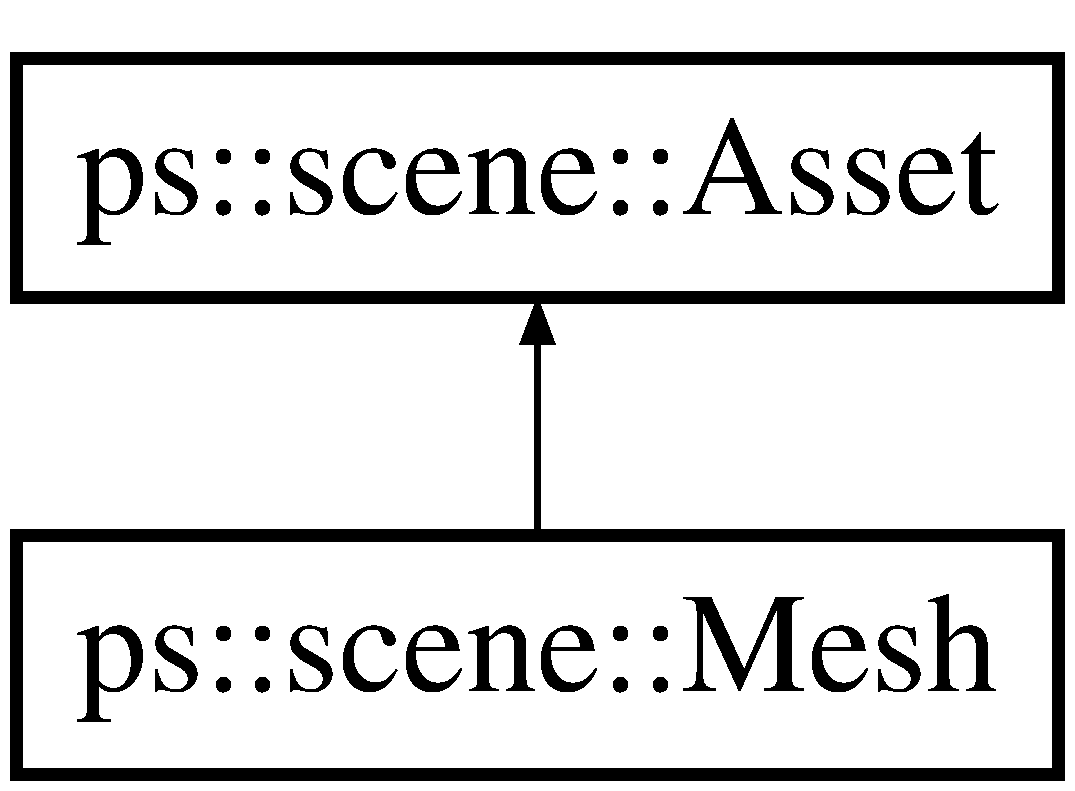
\includegraphics[height=2.000000cm]{classps_1_1scene_1_1Mesh}
\end{center}
\end{figure}
\subsection*{Public Member Functions}
\begin{DoxyCompactItemize}
\item 
\hypertarget{classps_1_1scene_1_1Mesh_a7d1542f47f2eca93df5ec0d8b0464820}{}{\bfseries Mesh} (const \hyperlink{classps_1_1base_1_1CAString}{Ansi\+Str} \&str\+File\+Path)\label{classps_1_1scene_1_1Mesh_a7d1542f47f2eca93df5ec0d8b0464820}

\item 
\hypertarget{classps_1_1scene_1_1Mesh_a02a7f043091f436683eced98557b7941}{}bool {\bfseries read} (const \hyperlink{classps_1_1base_1_1CAString}{Ansi\+Str} \&str\+File\+Path)\label{classps_1_1scene_1_1Mesh_a02a7f043091f436683eced98557b7941}

\item 
\hypertarget{classps_1_1scene_1_1Mesh_a07e0c38041091f0ec048a3e97afa7f98}{}bool {\bfseries store} (const \hyperlink{classps_1_1base_1_1CAString}{Ansi\+Str} \&str\+File\+Path)\label{classps_1_1scene_1_1Mesh_a07e0c38041091f0ec048a3e97afa7f98}

\item 
\hypertarget{classps_1_1scene_1_1Mesh_a85a3e2b850980c2bf6464cd52abe9034}{}void {\bfseries add\+Node} (\hyperlink{classps_1_1scene_1_1MeshNode}{Mesh\+Node} $\ast$lp\+Mesh\+Node)\label{classps_1_1scene_1_1Mesh_a85a3e2b850980c2bf6464cd52abe9034}

\item 
\hypertarget{classps_1_1scene_1_1Mesh_a17dce90c56ead670f4bafe8734b84dbe}{}\hyperlink{classps_1_1scene_1_1MeshNode}{Mesh\+Node} $\ast$ {\bfseries get\+Node} (int idx) const \label{classps_1_1scene_1_1Mesh_a17dce90c56ead670f4bafe8734b84dbe}

\item 
\hypertarget{classps_1_1scene_1_1Mesh_ab1a9ef3f67468e41acaf72740e40f6c5}{}\hyperlink{classps_1_1scene_1_1MeshNode}{Mesh\+Node} $\ast$ {\bfseries get\+Node} (const string \&name) const \label{classps_1_1scene_1_1Mesh_ab1a9ef3f67468e41acaf72740e40f6c5}

\item 
\hypertarget{classps_1_1scene_1_1Mesh_acc814ba6fc47832d2b112ab733883f57}{}U32 {\bfseries count\+Nodes} () const \label{classps_1_1scene_1_1Mesh_acc814ba6fc47832d2b112ab733883f57}

\item 
\hypertarget{classps_1_1scene_1_1Mesh_a27f2b76dbc292767eebf2b81eb030f4e}{}void {\bfseries add\+Mesh\+Material} (\hyperlink{classps_1_1scene_1_1MeshMaterial}{Mesh\+Material} $\ast$lp\+Material)\label{classps_1_1scene_1_1Mesh_a27f2b76dbc292767eebf2b81eb030f4e}

\item 
\hypertarget{classps_1_1scene_1_1Mesh_a3a5836d198af9ba40ecce0c3cd06dcf8}{}\hyperlink{classps_1_1scene_1_1MeshMaterial}{Mesh\+Material} $\ast$ {\bfseries get\+Material} (int idx) const \label{classps_1_1scene_1_1Mesh_a3a5836d198af9ba40ecce0c3cd06dcf8}

\item 
\hypertarget{classps_1_1scene_1_1Mesh_a8bd41c6aabd0e6531ba339010604a6ae}{}\hyperlink{classps_1_1scene_1_1MeshMaterial}{Mesh\+Material} $\ast$ {\bfseries get\+Material} (const string \&str\+Name) const \label{classps_1_1scene_1_1Mesh_a8bd41c6aabd0e6531ba339010604a6ae}

\item 
\hypertarget{classps_1_1scene_1_1Mesh_a0748028365d38a4d568f9d303ec1b611}{}U32 {\bfseries count\+Materials} () const \label{classps_1_1scene_1_1Mesh_a0748028365d38a4d568f9d303ec1b611}

\item 
\hypertarget{classps_1_1scene_1_1Mesh_a7a288493f2f3acedeeaa1397a5b65699}{}\hyperlink{classps_1_1base_1_1AABB}{A\+A\+B\+B} {\bfseries compute\+Bounding\+Box} () const \label{classps_1_1scene_1_1Mesh_a7a288493f2f3acedeeaa1397a5b65699}

\item 
\hypertarget{classps_1_1scene_1_1Mesh_af0140faaabe04e1f5692012b79444826}{}void {\bfseries compute\+Missing\+Normals} ()\label{classps_1_1scene_1_1Mesh_af0140faaabe04e1f5692012b79444826}

\item 
\hypertarget{classps_1_1scene_1_1Mesh_afd0ddc2e64ded35b9d368016b9ccdbd8}{}void {\bfseries move} (const \hyperlink{classps_1_1base_1_1Vec3}{vec3f} \&d)\label{classps_1_1scene_1_1Mesh_afd0ddc2e64ded35b9d368016b9ccdbd8}

\item 
\hypertarget{classps_1_1scene_1_1Mesh_a4ae686c746bd2897fcf201d7865b3935}{}void {\bfseries scale} (const \hyperlink{classps_1_1base_1_1Vec3}{vec3f} \&s)\label{classps_1_1scene_1_1Mesh_a4ae686c746bd2897fcf201d7865b3935}

\item 
\hypertarget{classps_1_1scene_1_1Mesh_a2c8a6bd2de6f9addcbe6e9dcf21d5abe}{}void {\bfseries rotate} (const \hyperlink{classps_1_1base_1_1Quaternion}{quat} \&q)\label{classps_1_1scene_1_1Mesh_a2c8a6bd2de6f9addcbe6e9dcf21d5abe}

\item 
\hypertarget{classps_1_1scene_1_1Mesh_ab7a98aaafffd3fd27d209150b2375aee}{}void {\bfseries fit\+To\+B\+Box} (const \hyperlink{classps_1_1base_1_1AABB}{A\+A\+B\+B} \&box)\label{classps_1_1scene_1_1Mesh_ab7a98aaafffd3fd27d209150b2375aee}

\end{DoxyCompactItemize}
\subsection*{Additional Inherited Members}


The documentation for this class was generated from the following files\+:\begin{DoxyCompactItemize}
\item 
/\+Users/pourya/\+Desktop/platform/repos/tetcutter/src/scene/surfacemesh.\+h\item 
/\+Users/pourya/\+Desktop/platform/repos/tetcutter/src/scene/surfacemesh.\+cpp\end{DoxyCompactItemize}

\hypertarget{classps_1_1scene_1_1MeshMaterial}{}\section{ps\+:\+:scene\+:\+:Mesh\+Material Class Reference}
\label{classps_1_1scene_1_1MeshMaterial}\index{ps\+::scene\+::\+Mesh\+Material@{ps\+::scene\+::\+Mesh\+Material}}


{\ttfamily \#include $<$surfacemesh.\+h$>$}

Inheritance diagram for ps\+:\+:scene\+:\+:Mesh\+Material\+:\begin{figure}[H]
\begin{center}
\leavevmode
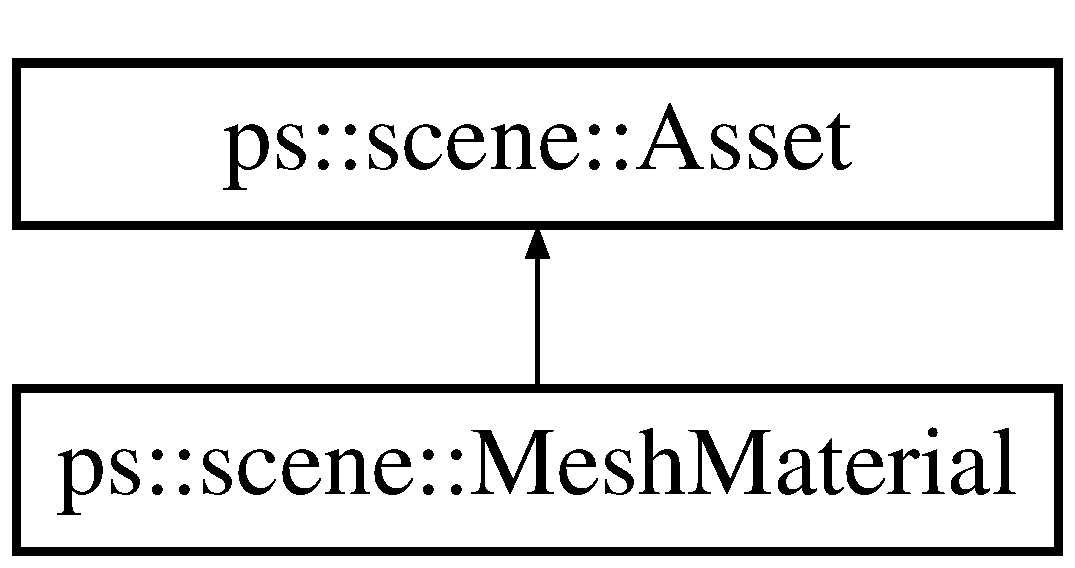
\includegraphics[height=2.000000cm]{classps_1_1scene_1_1MeshMaterial}
\end{center}
\end{figure}
\subsection*{Public Member Functions}
\begin{DoxyCompactItemize}
\item 
\hypertarget{classps_1_1scene_1_1MeshMaterial_a3d7c3aebc91885aa712ec612ed30b090}{}{\bfseries Mesh\+Material} (const string \&name)\label{classps_1_1scene_1_1MeshMaterial_a3d7c3aebc91885aa712ec612ed30b090}

\item 
\hypertarget{classps_1_1scene_1_1MeshMaterial_ab0b2b5fa06a02b936e5797cf4a0ad7ed}{}bool {\bfseries load} (const char $\ast$chr\+File\+Path)\label{classps_1_1scene_1_1MeshMaterial_ab0b2b5fa06a02b936e5797cf4a0ad7ed}

\item 
\hypertarget{classps_1_1scene_1_1MeshMaterial_a54c47d41769a5bcd4b4f356345c06598}{}bool {\bfseries store} (const char $\ast$chr\+File\+Path)\label{classps_1_1scene_1_1MeshMaterial_a54c47d41769a5bcd4b4f356345c06598}

\end{DoxyCompactItemize}
\subsection*{Public Attributes}
\begin{DoxyCompactItemize}
\item 
\hypertarget{classps_1_1scene_1_1MeshMaterial_ae151fde7758d65a02b6f19a8243c21d8}{}string {\bfseries str\+M\+T\+L\+Name}\label{classps_1_1scene_1_1MeshMaterial_ae151fde7758d65a02b6f19a8243c21d8}

\item 
\hypertarget{classps_1_1scene_1_1MeshMaterial_ab5e62b8a858dafcda1c52f3eb993207b}{}string {\bfseries str\+Tex\+Name}\label{classps_1_1scene_1_1MeshMaterial_ab5e62b8a858dafcda1c52f3eb993207b}

\item 
\hypertarget{classps_1_1scene_1_1MeshMaterial_afaab27da25ba4a50fe22f33b1c990789}{}\hyperlink{classps_1_1base_1_1Vec3}{vec3f} {\bfseries ambient}\label{classps_1_1scene_1_1MeshMaterial_afaab27da25ba4a50fe22f33b1c990789}

\item 
\hypertarget{classps_1_1scene_1_1MeshMaterial_a8c5bf5ce89d695a72900d924691bbc31}{}\hyperlink{classps_1_1base_1_1Vec3}{vec3f} {\bfseries diffused}\label{classps_1_1scene_1_1MeshMaterial_a8c5bf5ce89d695a72900d924691bbc31}

\item 
\hypertarget{classps_1_1scene_1_1MeshMaterial_a7fad2aa88cabdf56f3e4eb9f83b95c41}{}\hyperlink{classps_1_1base_1_1Vec3}{vec3f} {\bfseries specular}\label{classps_1_1scene_1_1MeshMaterial_a7fad2aa88cabdf56f3e4eb9f83b95c41}

\item 
\hypertarget{classps_1_1scene_1_1MeshMaterial_a1799cc04339c93e098ac172e34f74f95}{}float {\bfseries reflect}\label{classps_1_1scene_1_1MeshMaterial_a1799cc04339c93e098ac172e34f74f95}

\item 
\hypertarget{classps_1_1scene_1_1MeshMaterial_aa137fcdfd884692ced4138a3fbd62ab7}{}float {\bfseries refract}\label{classps_1_1scene_1_1MeshMaterial_aa137fcdfd884692ced4138a3fbd62ab7}

\item 
\hypertarget{classps_1_1scene_1_1MeshMaterial_a275716fbe88a754315b0966b7863a36e}{}float {\bfseries trans}\label{classps_1_1scene_1_1MeshMaterial_a275716fbe88a754315b0966b7863a36e}

\item 
\hypertarget{classps_1_1scene_1_1MeshMaterial_abd291e872acb8f7038e7018d92a17784}{}float {\bfseries shininess}\label{classps_1_1scene_1_1MeshMaterial_abd291e872acb8f7038e7018d92a17784}

\item 
\hypertarget{classps_1_1scene_1_1MeshMaterial_a65476012eb335f2fe6b1edc53c32cfec}{}float {\bfseries glossy}\label{classps_1_1scene_1_1MeshMaterial_a65476012eb335f2fe6b1edc53c32cfec}

\item 
\hypertarget{classps_1_1scene_1_1MeshMaterial_a7bcc08f3b02f6e00e975590aa871fb6b}{}float {\bfseries refract\+Index}\label{classps_1_1scene_1_1MeshMaterial_a7bcc08f3b02f6e00e975590aa871fb6b}

\item 
\hypertarget{classps_1_1scene_1_1MeshMaterial_a7d9a56ac3322d7ce53c22b13b1724169}{}int {\bfseries illumination\+Model}\label{classps_1_1scene_1_1MeshMaterial_a7d9a56ac3322d7ce53c22b13b1724169}

\end{DoxyCompactItemize}
\subsection*{Additional Inherited Members}


\subsection{Detailed Description}
structure holding a mesh material object 

The documentation for this class was generated from the following files\+:\begin{DoxyCompactItemize}
\item 
/\+Users/pourya/\+Desktop/platform/repos/tetcutter/src/scene/surfacemesh.\+h\item 
/\+Users/pourya/\+Desktop/platform/repos/tetcutter/src/scene/surfacemesh.\+cpp\end{DoxyCompactItemize}

\hypertarget{classps_1_1scene_1_1MeshNode}{}\section{ps\+:\+:scene\+:\+:Mesh\+Node Class Reference}
\label{classps_1_1scene_1_1MeshNode}\index{ps\+::scene\+::\+Mesh\+Node@{ps\+::scene\+::\+Mesh\+Node}}


{\ttfamily \#include $<$surfacemesh.\+h$>$}

\subsection*{Public Member Functions}
\begin{DoxyCompactItemize}
\item 
\hypertarget{classps_1_1scene_1_1MeshNode_a1ffab8f4eebb6e487b30e43099752c99}{}{\bfseries Mesh\+Node} (const string \&name)\label{classps_1_1scene_1_1MeshNode_a1ffab8f4eebb6e487b30e43099752c99}

\item 
\hypertarget{classps_1_1scene_1_1MeshNode_a08a8a5caa8021bcc68b14de1d7ceeaf5}{}{\bfseries Mesh\+Node} (const \hyperlink{classps_1_1scene_1_1MeshNode}{Mesh\+Node} $\ast$lp\+Node)\label{classps_1_1scene_1_1MeshNode_a08a8a5caa8021bcc68b14de1d7ceeaf5}

\item 
\hypertarget{classps_1_1scene_1_1MeshNode_af3acd683b56c5aec14ebf018517eba48}{}void {\bfseries init} ()\label{classps_1_1scene_1_1MeshNode_af3acd683b56c5aec14ebf018517eba48}

\item 
\hypertarget{classps_1_1scene_1_1MeshNode_a83f1d8c02d7e9d0608ff67a6b213c15f}{}bool {\bfseries readback\+Mesh\+V3\+T3} (U32 \&ct\+Vertices, vector$<$ float $>$ \&vertices, U32 \&ct\+Triangles, vector$<$ U32 $>$ \&elements)\label{classps_1_1scene_1_1MeshNode_a83f1d8c02d7e9d0608ff67a6b213c15f}

\item 
int \hyperlink{classps_1_1scene_1_1MeshNode_a2a8293f22a8add94d330daff6bc2bd7b}{add} (const \hyperlink{classps_1_1base_1_1Vec3}{vec3f} \&v, G\+L\+Buffer\+Type vat=gbt\+Position, int step=3)
\item 
\hypertarget{classps_1_1scene_1_1MeshNode_ae646caed0e8b1bfeb41a2b832a83c8b7}{}int {\bfseries add} (const \hyperlink{classps_1_1base_1_1Vec4}{vec4f} \&v, G\+L\+Buffer\+Type vat=gbt\+Position, int step=4)\label{classps_1_1scene_1_1MeshNode_ae646caed0e8b1bfeb41a2b832a83c8b7}

\item 
\hypertarget{classps_1_1scene_1_1MeshNode_a4ec9d77bddc3f2e12e40de75da214f0b}{}int {\bfseries add} (const vector$<$ float $>$ \&arr\+Values, G\+L\+Buffer\+Type vat=gbt\+Position, int step=3)\label{classps_1_1scene_1_1MeshNode_a4ec9d77bddc3f2e12e40de75da214f0b}

\item 
\hypertarget{classps_1_1scene_1_1MeshNode_a334b1a7c3117a44c49f4268c62f17eaa}{}void {\bfseries set\+Vertex\+Attrib} (const vector$<$ float $>$ \&arr\+Attribs, G\+L\+Buffer\+Type vat=gbt\+Position, int step=3)\label{classps_1_1scene_1_1MeshNode_a334b1a7c3117a44c49f4268c62f17eaa}

\item 
\hypertarget{classps_1_1scene_1_1MeshNode_a8767136311d4c299bef09e9e74d269fc}{}int {\bfseries add\+Vertex} (const \hyperlink{classps_1_1base_1_1Vec3}{vec3f} \&v)\label{classps_1_1scene_1_1MeshNode_a8767136311d4c299bef09e9e74d269fc}

\item 
\hypertarget{classps_1_1scene_1_1MeshNode_a56419c311e60f061c252de743ddee782}{}int {\bfseries add\+Normal} (const \hyperlink{classps_1_1base_1_1Vec3}{vec3f} \&n)\label{classps_1_1scene_1_1MeshNode_a56419c311e60f061c252de743ddee782}

\item 
\hypertarget{classps_1_1scene_1_1MeshNode_a2e9d316247bac977d6b2ed462ae529a0}{}int {\bfseries add\+Tex\+Coord2} (const \hyperlink{classps_1_1base_1_1Vec2}{vec2f} \&t)\label{classps_1_1scene_1_1MeshNode_a2e9d316247bac977d6b2ed462ae529a0}

\item 
\hypertarget{classps_1_1scene_1_1MeshNode_a224511681ccb6008bff96ed34f9f2f47}{}int {\bfseries add\+Tex\+Coord3} (const \hyperlink{classps_1_1base_1_1Vec3}{vec3f} \&t)\label{classps_1_1scene_1_1MeshNode_a224511681ccb6008bff96ed34f9f2f47}

\item 
\hypertarget{classps_1_1scene_1_1MeshNode_ac9c6f221071dd22c88deb937afb5f4a9}{}void {\bfseries add\+Triangle} (U32 tri\mbox{[}3\mbox{]})\label{classps_1_1scene_1_1MeshNode_ac9c6f221071dd22c88deb937afb5f4a9}

\item 
\hypertarget{classps_1_1scene_1_1MeshNode_a8736493b1bc007c0f924adc83c43c9e7}{}void {\bfseries add\+Quad} (U32 quad\mbox{[}4\mbox{]})\label{classps_1_1scene_1_1MeshNode_a8736493b1bc007c0f924adc83c43c9e7}

\item 
\hypertarget{classps_1_1scene_1_1MeshNode_a5e1b52007eec9bf2310d5c8476fa7901}{}void {\bfseries add\+Face\+Index} (U32 index)\label{classps_1_1scene_1_1MeshNode_a5e1b52007eec9bf2310d5c8476fa7901}

\item 
\hypertarget{classps_1_1scene_1_1MeshNode_afcd2c042b979b2275880054b77b79a9c}{}void {\bfseries set\+Face\+Indices} (const vector$<$ U32 $>$ \&arr\+Faces, int unit\+Face)\label{classps_1_1scene_1_1MeshNode_afcd2c042b979b2275880054b77b79a9c}

\item 
int \hyperlink{classps_1_1scene_1_1MeshNode_a5ae2786a600ec3a343b0d848da121842}{count\+Face\+Index\+Errors} () const 
\item 
\hypertarget{classps_1_1scene_1_1MeshNode_ae776587abb773e23135a99ea2a5edf1b}{}void \hyperlink{classps_1_1scene_1_1MeshNode_ae776587abb773e23135a99ea2a5edf1b}{compute\+Vertex\+Normals\+From\+Faces} ()\label{classps_1_1scene_1_1MeshNode_ae776587abb773e23135a99ea2a5edf1b}

\begin{DoxyCompactList}\small\item\em compute\+Vertex\+Normals\+From\+Faces compute one normal per each vertex by summing up all adjacent face normals and normalize it. \end{DoxyCompactList}\item 
\hypertarget{classps_1_1scene_1_1MeshNode_a985cb7e99f593a7f30da05ab0539bed1}{}U32 {\bfseries count\+Vertices} () const \label{classps_1_1scene_1_1MeshNode_a985cb7e99f593a7f30da05ab0539bed1}

\item 
\hypertarget{classps_1_1scene_1_1MeshNode_aba0879a4d3bb3322b2d8b6ccd06a9066}{}U32 {\bfseries count\+Colors} () const \label{classps_1_1scene_1_1MeshNode_aba0879a4d3bb3322b2d8b6ccd06a9066}

\item 
\hypertarget{classps_1_1scene_1_1MeshNode_a1db603a096bc9262969ae7c5367a5edb}{}U32 {\bfseries count\+Normals} () const \label{classps_1_1scene_1_1MeshNode_a1db603a096bc9262969ae7c5367a5edb}

\item 
\hypertarget{classps_1_1scene_1_1MeshNode_af3fae6362d64ff0415da2f5544209e17}{}U32 {\bfseries count\+Faces} () const \label{classps_1_1scene_1_1MeshNode_af3fae6362d64ff0415da2f5544209e17}

\item 
\hypertarget{classps_1_1scene_1_1MeshNode_ab49145c691c1895f8ff22541f9647324}{}U32 {\bfseries count\+Tex\+Coords} () const \label{classps_1_1scene_1_1MeshNode_ab49145c691c1895f8ff22541f9647324}

\item 
U32 \hyperlink{classps_1_1scene_1_1MeshNode_aa3ac3b3ac130454dba6d2507a47e1586}{get\+Vertex\+Stride} () const 
\item 
\hypertarget{classps_1_1scene_1_1MeshNode_ad1a9aeeaf8b1d54916ab73669ca05f03}{}U32 {\bfseries get\+Normal\+Stride} () const \label{classps_1_1scene_1_1MeshNode_ad1a9aeeaf8b1d54916ab73669ca05f03}

\item 
\hypertarget{classps_1_1scene_1_1MeshNode_a4f05fa3565d63fe4a93cbf9fd32259f8}{}U32 {\bfseries get\+Face\+Stride} () const \label{classps_1_1scene_1_1MeshNode_a4f05fa3565d63fe4a93cbf9fd32259f8}

\item 
\hypertarget{classps_1_1scene_1_1MeshNode_a40fcb70031ecabe90b864f0321404967}{}\hyperlink{classps_1_1base_1_1Vec3}{vec3f} {\bfseries get\+Vertex} (int idx\+Vertex) const \label{classps_1_1scene_1_1MeshNode_a40fcb70031ecabe90b864f0321404967}

\item 
\hypertarget{classps_1_1scene_1_1MeshNode_ad9e2dc6ac318536b6d4ca35c68d9600a}{}\hyperlink{classps_1_1base_1_1Vec3}{vec3f} {\bfseries get\+Normal} (int idx\+Vertex) const \label{classps_1_1scene_1_1MeshNode_ad9e2dc6ac318536b6d4ca35c68d9600a}

\item 
\hypertarget{classps_1_1scene_1_1MeshNode_a3829ff7e073b818080e43ae96358dc68}{}\hyperlink{classps_1_1base_1_1Vec2}{vec2f} {\bfseries get\+Tex\+Coord2} (int idx\+Vertex) const \label{classps_1_1scene_1_1MeshNode_a3829ff7e073b818080e43ae96358dc68}

\item 
\hypertarget{classps_1_1scene_1_1MeshNode_a7a26cafa1e804749d464b990c2594070}{}\hyperlink{classps_1_1base_1_1Vec3}{vec3f} {\bfseries get\+Tex\+Coord3} (int idx\+Vertex) const \label{classps_1_1scene_1_1MeshNode_a7a26cafa1e804749d464b990c2594070}

\item 
\hypertarget{classps_1_1scene_1_1MeshNode_a2976bb4ccbce4f8b661f3dae7050e830}{}\hyperlink{classps_1_1scene_1_1MeshMaterial}{Mesh\+Material} $\ast$ {\bfseries get\+Material} () const \label{classps_1_1scene_1_1MeshNode_a2976bb4ccbce4f8b661f3dae7050e830}

\item 
\hypertarget{classps_1_1scene_1_1MeshNode_a4c24fee166eecbe5cd667212c9223c2b}{}void {\bfseries set\+Material} (\hyperlink{classps_1_1scene_1_1MeshMaterial}{Mesh\+Material} $\ast$a\+Material)\label{classps_1_1scene_1_1MeshNode_a4c24fee166eecbe5cd667212c9223c2b}

\item 
\hypertarget{classps_1_1scene_1_1MeshNode_a422539466260f9d3c08b5411e64b934f}{}\hyperlink{classps_1_1base_1_1AABB}{A\+A\+B\+B} {\bfseries compute\+Bounding\+Box} () const \label{classps_1_1scene_1_1MeshNode_a422539466260f9d3c08b5411e64b934f}

\item 
\hypertarget{classps_1_1scene_1_1MeshNode_a7ece00736c911801762bc10fdca07f19}{}string {\bfseries get\+Name} () const \label{classps_1_1scene_1_1MeshNode_a7ece00736c911801762bc10fdca07f19}

\item 
\hypertarget{classps_1_1scene_1_1MeshNode_a58993714a990f817da49d5f8b96cd28c}{}void {\bfseries set\+Name} (const string \&str\+Name)\label{classps_1_1scene_1_1MeshNode_a58993714a990f817da49d5f8b96cd28c}

\item 
\hypertarget{classps_1_1scene_1_1MeshNode_ad2690cc20b520deef7ddb75e9e732bc1}{}U8 {\bfseries get\+Unit\+Vertex} () const \label{classps_1_1scene_1_1MeshNode_ad2690cc20b520deef7ddb75e9e732bc1}

\item 
\hypertarget{classps_1_1scene_1_1MeshNode_a314b19aa4f8f2f318e65d7a256d9b13f}{}U8 {\bfseries get\+Unit\+Normal} () const \label{classps_1_1scene_1_1MeshNode_a314b19aa4f8f2f318e65d7a256d9b13f}

\item 
\hypertarget{classps_1_1scene_1_1MeshNode_a2898527c4ed539aee68f7cd3823d65d9}{}U8 {\bfseries get\+Unit\+Color} () const \label{classps_1_1scene_1_1MeshNode_a2898527c4ed539aee68f7cd3823d65d9}

\item 
\hypertarget{classps_1_1scene_1_1MeshNode_a2558ab01df176a9253322c96d058b976}{}U8 {\bfseries get\+Unit\+Tex\+Coord} () const \label{classps_1_1scene_1_1MeshNode_a2558ab01df176a9253322c96d058b976}

\item 
\hypertarget{classps_1_1scene_1_1MeshNode_a849d8997220a3f375b04325b9f9cff7a}{}U8 {\bfseries get\+Unit\+Face} () const \label{classps_1_1scene_1_1MeshNode_a849d8997220a3f375b04325b9f9cff7a}

\item 
\hypertarget{classps_1_1scene_1_1MeshNode_ad00f6c2640f8f1858e685f1ce8fd01a8}{}void {\bfseries set\+Unit\+Face} (U8 s)\label{classps_1_1scene_1_1MeshNode_ad00f6c2640f8f1858e685f1ce8fd01a8}

\item 
\hypertarget{classps_1_1scene_1_1MeshNode_a00a0b531ce934e18afdb7f668b2e419f}{}void {\bfseries get\+Vertex\+Attrib} (U32 \&count, vector$<$ float $>$ \&arr\+Attribs, G\+L\+Buffer\+Type vat) const \label{classps_1_1scene_1_1MeshNode_a00a0b531ce934e18afdb7f668b2e419f}

\item 
\hypertarget{classps_1_1scene_1_1MeshNode_aa43d632903b7ebb08d6ca5520d98dcb1}{}void {\bfseries get\+Faces} (U32 \&count, vector$<$ U32 $>$ \&faces) const \label{classps_1_1scene_1_1MeshNode_aa43d632903b7ebb08d6ca5520d98dcb1}

\item 
\hypertarget{classps_1_1scene_1_1MeshNode_a3644efcb68695c76cc1979b2d84ae575}{}const vector$<$ float $>$ \& {\bfseries vertices} () const \label{classps_1_1scene_1_1MeshNode_a3644efcb68695c76cc1979b2d84ae575}

\item 
\hypertarget{classps_1_1scene_1_1MeshNode_a220bd015975bc9ad09f7cd30e5edb38f}{}const vector$<$ float $>$ \& {\bfseries normals} () const \label{classps_1_1scene_1_1MeshNode_a220bd015975bc9ad09f7cd30e5edb38f}

\item 
\hypertarget{classps_1_1scene_1_1MeshNode_ad13c76f480a5d4fa3835252e83744389}{}const vector$<$ float $>$ \& {\bfseries colors} () const \label{classps_1_1scene_1_1MeshNode_ad13c76f480a5d4fa3835252e83744389}

\item 
\hypertarget{classps_1_1scene_1_1MeshNode_a14335fa698f48c9f507719a731b964d3}{}const vector$<$ float $>$ \& {\bfseries texcoords} () const \label{classps_1_1scene_1_1MeshNode_a14335fa698f48c9f507719a731b964d3}

\item 
\hypertarget{classps_1_1scene_1_1MeshNode_a6eb251b5ad51cd1a9c91d244ee51f7b5}{}const vector$<$ U32 $>$ \& {\bfseries face\+Elements} () const \label{classps_1_1scene_1_1MeshNode_a6eb251b5ad51cd1a9c91d244ee51f7b5}

\item 
void \hyperlink{classps_1_1scene_1_1MeshNode_a402258ff6c02b502066391b2f45cc1a3}{move} (const \hyperlink{classps_1_1base_1_1Vec3}{vec3f} \&d)
\item 
\hypertarget{classps_1_1scene_1_1MeshNode_a139330df65d3b518c3a8027c64b76f72}{}void {\bfseries scale} (const \hyperlink{classps_1_1base_1_1Vec3}{vec3f} \&s)\label{classps_1_1scene_1_1MeshNode_a139330df65d3b518c3a8027c64b76f72}

\item 
\hypertarget{classps_1_1scene_1_1MeshNode_aeee4bb1242563f57d091746089c44090}{}void {\bfseries rotate} (const \hyperlink{classps_1_1base_1_1Quaternion}{quat} \&q)\label{classps_1_1scene_1_1MeshNode_aeee4bb1242563f57d091746089c44090}

\item 
\hypertarget{classps_1_1scene_1_1MeshNode_aa010507baafa5f58b3c36a0b5b749b87}{}void {\bfseries fit\+To\+B\+Box} (const \hyperlink{classps_1_1base_1_1AABB}{A\+A\+B\+B} \&box)\label{classps_1_1scene_1_1MeshNode_aa010507baafa5f58b3c36a0b5b749b87}

\end{DoxyCompactItemize}
\subsection*{Protected Attributes}
\begin{DoxyCompactItemize}
\item 
\hypertarget{classps_1_1scene_1_1MeshNode_a1b2d946bc514452b39c2abee19ce3416}{}std\+::vector$<$ float $>$ {\bfseries m\+\_\+arr\+Vertices}\label{classps_1_1scene_1_1MeshNode_a1b2d946bc514452b39c2abee19ce3416}

\item 
\hypertarget{classps_1_1scene_1_1MeshNode_ae3f478aaf92026791d7f017994c799d8}{}std\+::vector$<$ float $>$ {\bfseries m\+\_\+arr\+Normals}\label{classps_1_1scene_1_1MeshNode_ae3f478aaf92026791d7f017994c799d8}

\item 
\hypertarget{classps_1_1scene_1_1MeshNode_af99ba6439e4d8a6797a03c17780206ed}{}std\+::vector$<$ float $>$ {\bfseries m\+\_\+arr\+Colors}\label{classps_1_1scene_1_1MeshNode_af99ba6439e4d8a6797a03c17780206ed}

\item 
\hypertarget{classps_1_1scene_1_1MeshNode_a985972268af3b8a730a2b9f7ee6b1e35}{}std\+::vector$<$ float $>$ {\bfseries m\+\_\+arr\+Tex\+Coords}\label{classps_1_1scene_1_1MeshNode_a985972268af3b8a730a2b9f7ee6b1e35}

\item 
\hypertarget{classps_1_1scene_1_1MeshNode_ac4a941f49efe920d1495a40bd13e62dc}{}std\+::vector$<$ U32 $>$ {\bfseries m\+\_\+arr\+Indices}\label{classps_1_1scene_1_1MeshNode_ac4a941f49efe920d1495a40bd13e62dc}

\item 
\hypertarget{classps_1_1scene_1_1MeshNode_a596b0d0253ccde3015bd749097b3cf27}{}string {\bfseries m\+\_\+str\+Node\+Name}\label{classps_1_1scene_1_1MeshNode_a596b0d0253ccde3015bd749097b3cf27}

\item 
\hypertarget{classps_1_1scene_1_1MeshNode_ac798f6e24021251b8290e14416b424ff}{}U8 {\bfseries m\+\_\+sz\+Unit\+Vertex}\label{classps_1_1scene_1_1MeshNode_ac798f6e24021251b8290e14416b424ff}

\item 
\hypertarget{classps_1_1scene_1_1MeshNode_a138d8ab801fc1007a872961edfa16a60}{}U8 {\bfseries m\+\_\+sz\+Unit\+Color}\label{classps_1_1scene_1_1MeshNode_a138d8ab801fc1007a872961edfa16a60}

\item 
\hypertarget{classps_1_1scene_1_1MeshNode_a43eccfcb1b1781229827a2946be4691a}{}U8 {\bfseries m\+\_\+sz\+Unit\+Tex\+Coord}\label{classps_1_1scene_1_1MeshNode_a43eccfcb1b1781229827a2946be4691a}

\item 
\hypertarget{classps_1_1scene_1_1MeshNode_a1807d198386660544ecda3051a6fbdae}{}U8 {\bfseries m\+\_\+sz\+Unit\+Face}\label{classps_1_1scene_1_1MeshNode_a1807d198386660544ecda3051a6fbdae}

\item 
\hypertarget{classps_1_1scene_1_1MeshNode_a7905534a2861eaedef4dc2d8dfc0cff5}{}\hyperlink{classps_1_1scene_1_1MeshMaterial}{Mesh\+Material} $\ast$ {\bfseries m\+\_\+lp\+Material}\label{classps_1_1scene_1_1MeshNode_a7905534a2861eaedef4dc2d8dfc0cff5}

\end{DoxyCompactItemize}


\subsection{Detailed Description}
\hyperlink{classps_1_1scene_1_1MeshNode}{Mesh\+Node} represents a single node in our mesh file. It is complete mesh by itself. 

\subsection{Member Function Documentation}
\hypertarget{classps_1_1scene_1_1MeshNode_a2a8293f22a8add94d330daff6bc2bd7b}{}\index{ps\+::scene\+::\+Mesh\+Node@{ps\+::scene\+::\+Mesh\+Node}!add@{add}}
\index{add@{add}!ps\+::scene\+::\+Mesh\+Node@{ps\+::scene\+::\+Mesh\+Node}}
\subsubsection[{add(const vec3f \&v, G\+L\+Buffer\+Type vat=gbt\+Position, int step=3)}]{\setlength{\rightskip}{0pt plus 5cm}int ps\+::scene\+::\+Mesh\+Node\+::add (
\begin{DoxyParamCaption}
\item[{const {\bf vec3f} \&}]{v, }
\item[{G\+L\+Buffer\+Type}]{vat = {\ttfamily gbtPosition}, }
\item[{int}]{step = {\ttfamily 3}}
\end{DoxyParamCaption}
)}\label{classps_1_1scene_1_1MeshNode_a2a8293f22a8add94d330daff6bc2bd7b}
Adds a vec3f v to the destination buffer dest. \begin{DoxyReturn}{Returns}
designated index of added vertex. This index is the actual vertex number not the position in the float array. The position in the float array can be computed as index x sz\+Unit\+Vertex 
\end{DoxyReturn}
\hypertarget{classps_1_1scene_1_1MeshNode_a5ae2786a600ec3a343b0d848da121842}{}\index{ps\+::scene\+::\+Mesh\+Node@{ps\+::scene\+::\+Mesh\+Node}!count\+Face\+Index\+Errors@{count\+Face\+Index\+Errors}}
\index{count\+Face\+Index\+Errors@{count\+Face\+Index\+Errors}!ps\+::scene\+::\+Mesh\+Node@{ps\+::scene\+::\+Mesh\+Node}}
\subsubsection[{count\+Face\+Index\+Errors() const }]{\setlength{\rightskip}{0pt plus 5cm}int ps\+::scene\+::\+Mesh\+Node\+::count\+Face\+Index\+Errors (
\begin{DoxyParamCaption}
{}
\end{DoxyParamCaption}
) const}\label{classps_1_1scene_1_1MeshNode_a5ae2786a600ec3a343b0d848da121842}
Checks all face indices for invalid values \begin{DoxyReturn}{Returns}
number of indices found out of range 
\end{DoxyReturn}
\hypertarget{classps_1_1scene_1_1MeshNode_aa3ac3b3ac130454dba6d2507a47e1586}{}\index{ps\+::scene\+::\+Mesh\+Node@{ps\+::scene\+::\+Mesh\+Node}!get\+Vertex\+Stride@{get\+Vertex\+Stride}}
\index{get\+Vertex\+Stride@{get\+Vertex\+Stride}!ps\+::scene\+::\+Mesh\+Node@{ps\+::scene\+::\+Mesh\+Node}}
\subsubsection[{get\+Vertex\+Stride() const }]{\setlength{\rightskip}{0pt plus 5cm}U32 ps\+::scene\+::\+Mesh\+Node\+::get\+Vertex\+Stride (
\begin{DoxyParamCaption}
{}
\end{DoxyParamCaption}
) const\hspace{0.3cm}{\ttfamily [inline]}}\label{classps_1_1scene_1_1MeshNode_aa3ac3b3ac130454dba6d2507a47e1586}
returns unit vertex memory stride in bytes \hypertarget{classps_1_1scene_1_1MeshNode_a402258ff6c02b502066391b2f45cc1a3}{}\index{ps\+::scene\+::\+Mesh\+Node@{ps\+::scene\+::\+Mesh\+Node}!move@{move}}
\index{move@{move}!ps\+::scene\+::\+Mesh\+Node@{ps\+::scene\+::\+Mesh\+Node}}
\subsubsection[{move(const vec3f \&d)}]{\setlength{\rightskip}{0pt plus 5cm}void ps\+::scene\+::\+Mesh\+Node\+::move (
\begin{DoxyParamCaption}
\item[{const {\bf vec3f} \&}]{d}
\end{DoxyParamCaption}
)}\label{classps_1_1scene_1_1MeshNode_a402258ff6c02b502066391b2f45cc1a3}
Move the entire mesh to a new location 

The documentation for this class was generated from the following files\+:\begin{DoxyCompactItemize}
\item 
/\+Users/pourya/\+Desktop/platform/repos/tetcutter/src/scene/surfacemesh.\+h\item 
/\+Users/pourya/\+Desktop/platform/repos/tetcutter/src/scene/surfacemesh.\+cpp\end{DoxyCompactItemize}

\hypertarget{classps_1_1base_1_1MovingAvg}{}\section{ps\+:\+:base\+:\+:Moving\+Avg$<$ T, length $>$ Class Template Reference}
\label{classps_1_1base_1_1MovingAvg}\index{ps\+::base\+::\+Moving\+Avg$<$ T, length $>$@{ps\+::base\+::\+Moving\+Avg$<$ T, length $>$}}
\subsection*{Public Types}
\begin{DoxyCompactItemize}
\item 
\hypertarget{classps_1_1base_1_1MovingAvg_ac2b80dc299c74872fd6aebd26ac30594}{}typedef T {\bfseries V\+A\+L\+U\+E\+T\+Y\+P\+E}\label{classps_1_1base_1_1MovingAvg_ac2b80dc299c74872fd6aebd26ac30594}

\end{DoxyCompactItemize}
\subsection*{Public Member Functions}
\begin{DoxyCompactItemize}
\item 
\hypertarget{classps_1_1base_1_1MovingAvg_a53892c1576ce47fba201a9d5fe77ad2b}{}void {\bfseries add\+Value} (T v)\label{classps_1_1base_1_1MovingAvg_a53892c1576ce47fba201a9d5fe77ad2b}

\item 
\hypertarget{classps_1_1base_1_1MovingAvg_a855a97e7b46d6ede2caa4c79edfef6fc}{}T {\bfseries get\+Value} (int idx) const \label{classps_1_1base_1_1MovingAvg_a855a97e7b46d6ede2caa4c79edfef6fc}

\item 
\hypertarget{classps_1_1base_1_1MovingAvg_ac56814bf4f62bdb3e91a09d8def83567}{}T {\bfseries get\+Average} () const \label{classps_1_1base_1_1MovingAvg_ac56814bf4f62bdb3e91a09d8def83567}

\item 
\hypertarget{classps_1_1base_1_1MovingAvg_abd2fa9d8a6a40f25cf788bcbcc0b2c9f}{}T {\bfseries get\+Current} () const \label{classps_1_1base_1_1MovingAvg_abd2fa9d8a6a40f25cf788bcbcc0b2c9f}

\item 
\hypertarget{classps_1_1base_1_1MovingAvg_a23b828dec96570a0f660b16a4933ffce}{}int {\bfseries get\+Window\+Size} ()\label{classps_1_1base_1_1MovingAvg_a23b828dec96570a0f660b16a4933ffce}

\end{DoxyCompactItemize}


The documentation for this class was generated from the following file\+:\begin{DoxyCompactItemize}
\item 
/\+Users/pourya/\+Desktop/platform/repos/tetcutter/src/base/movingavg.\+h\end{DoxyCompactItemize}

\hypertarget{classps_1_1elastic_1_1NODE}{}\section{ps\+:\+:elastic\+:\+:N\+O\+D\+E Class Reference}
\label{classps_1_1elastic_1_1NODE}\index{ps\+::elastic\+::\+N\+O\+D\+E@{ps\+::elastic\+::\+N\+O\+D\+E}}
\subsection*{Public Member Functions}
\begin{DoxyCompactItemize}
\item 
\hypertarget{classps_1_1elastic_1_1NODE_aa69fa9845a0c9308000a51a1b90a04f1}{}\hyperlink{classps_1_1elastic_1_1NODE}{N\+O\+D\+E} \& {\bfseries operator=} (const \hyperlink{classps_1_1elastic_1_1NODE}{N\+O\+D\+E} \&A)\label{classps_1_1elastic_1_1NODE_aa69fa9845a0c9308000a51a1b90a04f1}

\end{DoxyCompactItemize}
\subsection*{Public Attributes}
\begin{DoxyCompactItemize}
\item 
\hypertarget{classps_1_1elastic_1_1NODE_a6a3c621ea0ec87a55611c95f8cb1b7ca}{}\hyperlink{classps_1_1base_1_1Vec3}{vec3d} {\bfseries pos}\label{classps_1_1elastic_1_1NODE_a6a3c621ea0ec87a55611c95f8cb1b7ca}

\item 
\hypertarget{classps_1_1elastic_1_1NODE_ad6f2065a2d151d32bee55b1da3a26519}{}\hyperlink{classps_1_1base_1_1Vec3}{vec3d} {\bfseries restpos}\label{classps_1_1elastic_1_1NODE_ad6f2065a2d151d32bee55b1da3a26519}

\end{DoxyCompactItemize}


The documentation for this class was generated from the following file\+:\begin{DoxyCompactItemize}
\item 
/\+Users/pourya/\+Desktop/platform/repos/tetcutter/src/elastic/volmeshentities.\+h\end{DoxyCompactItemize}

\hypertarget{classps_1_1elastic_1_1NodeLink}{}\section{ps\+:\+:elastic\+:\+:Node\+Link Class Reference}
\label{classps_1_1elastic_1_1NodeLink}\index{ps\+::elastic\+::\+Node\+Link@{ps\+::elastic\+::\+Node\+Link}}
Inheritance diagram for ps\+:\+:elastic\+:\+:Node\+Link\+:\begin{figure}[H]
\begin{center}
\leavevmode
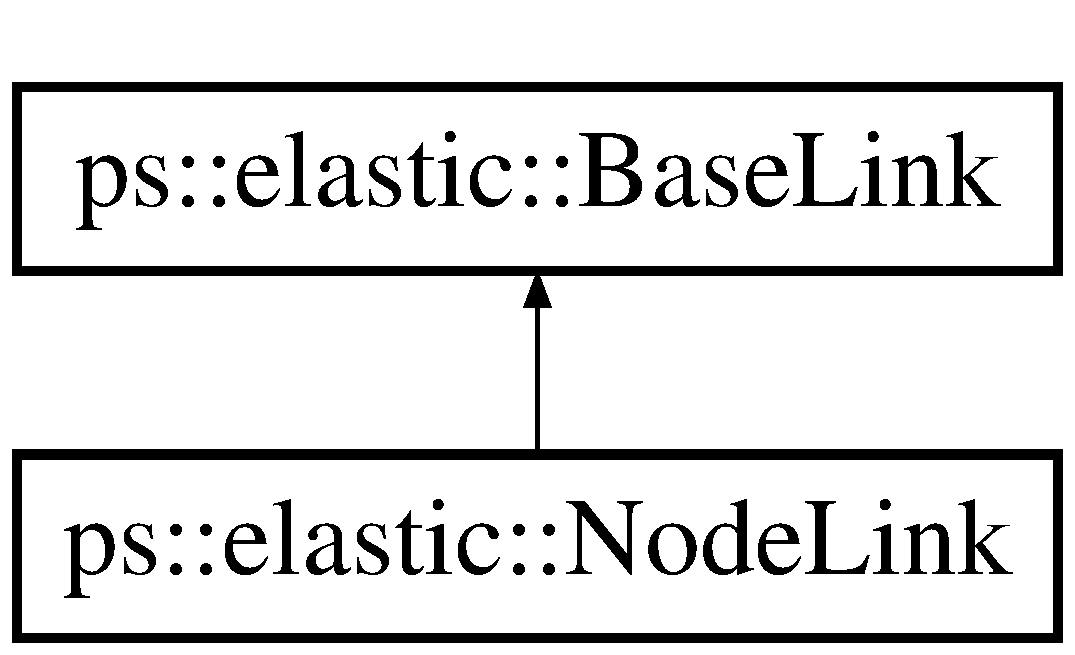
\includegraphics[height=2.000000cm]{classps_1_1elastic_1_1NodeLink}
\end{center}
\end{figure}
\subsection*{Static Public Member Functions}
\begin{DoxyCompactItemize}
\item 
\hypertarget{classps_1_1elastic_1_1NodeLink_aec4721a2587ab7fa6aadd737358b6321}{}static \hyperlink{classps_1_1elastic_1_1NodeLink}{Node\+Link} {\bfseries create} (U32 idx)\label{classps_1_1elastic_1_1NodeLink_aec4721a2587ab7fa6aadd737358b6321}

\end{DoxyCompactItemize}
\subsection*{Additional Inherited Members}


The documentation for this class was generated from the following file\+:\begin{DoxyCompactItemize}
\item 
/\+Users/pourya/\+Desktop/platform/repos/tetcutter/src/elastic/volmeshentities.\+h\end{DoxyCompactItemize}

\hypertarget{structps_1_1NoLogging}{}\section{ps\+:\+:No\+Logging Struct Reference}
\label{structps_1_1NoLogging}\index{ps\+::\+No\+Logging@{ps\+::\+No\+Logging}}
\subsection*{Static Public Member Functions}
\begin{DoxyCompactItemize}
\item 
\hypertarget{structps_1_1NoLogging_a7c8a6cb1444673346df5fe95572d85f8}{}static void {\bfseries Log\+Arg1} (const char $\ast$message, const char $\ast$arg1)\label{structps_1_1NoLogging_a7c8a6cb1444673346df5fe95572d85f8}

\end{DoxyCompactItemize}


The documentation for this struct was generated from the following file\+:\begin{DoxyCompactItemize}
\item 
/\+Users/pourya/\+Desktop/platform/repos/tetcutter/src/base/resourcemanager.\+h\end{DoxyCompactItemize}

\hypertarget{structps_1_1NoopInsertRemoveBySafeDelete}{}\section{ps\+:\+:Noop\+Insert\+Remove\+By\+Safe\+Delete$<$ T $>$ Struct Template Reference}
\label{structps_1_1NoopInsertRemoveBySafeDelete}\index{ps\+::\+Noop\+Insert\+Remove\+By\+Safe\+Delete$<$ T $>$@{ps\+::\+Noop\+Insert\+Remove\+By\+Safe\+Delete$<$ T $>$}}
\subsection*{Static Public Member Functions}
\begin{DoxyCompactItemize}
\item 
\hypertarget{structps_1_1NoopInsertRemoveBySafeDelete_a5c4457d7fc123c020b9a0710739296b9}{}static void {\bfseries Insert} (T element)\label{structps_1_1NoopInsertRemoveBySafeDelete_a5c4457d7fc123c020b9a0710739296b9}

\item 
\hypertarget{structps_1_1NoopInsertRemoveBySafeDelete_a78037c5610a765a6c3c2288635c5e988}{}static void {\bfseries Remove} (T element)\label{structps_1_1NoopInsertRemoveBySafeDelete_a78037c5610a765a6c3c2288635c5e988}

\end{DoxyCompactItemize}


The documentation for this struct was generated from the following file\+:\begin{DoxyCompactItemize}
\item 
/\+Users/pourya/\+Desktop/platform/repos/tetcutter/src/base/resourcemanager.\+h\end{DoxyCompactItemize}

\hypertarget{classps_1_1PRIVATE_1_1placeholder}{}\section{ps\+:\+:P\+R\+I\+V\+A\+T\+E\+:\+:placeholder Class Reference}
\label{classps_1_1PRIVATE_1_1placeholder}\index{ps\+::\+P\+R\+I\+V\+A\+T\+E\+::placeholder@{ps\+::\+P\+R\+I\+V\+A\+T\+E\+::placeholder}}
Inheritance diagram for ps\+:\+:P\+R\+I\+V\+A\+T\+E\+:\+:placeholder\+:\begin{figure}[H]
\begin{center}
\leavevmode
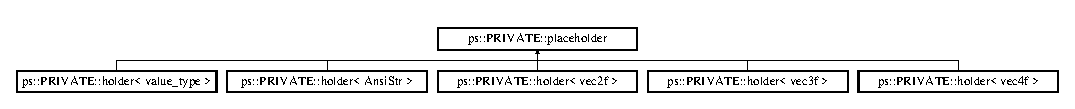
\includegraphics[height=1.022831cm]{classps_1_1PRIVATE_1_1placeholder}
\end{center}
\end{figure}
\subsection*{Public Member Functions}
\begin{DoxyCompactItemize}
\item 
\hypertarget{classps_1_1PRIVATE_1_1placeholder_a9adbf80e1db70fd00b277caa989562d0}{}virtual const std\+::type\+\_\+info \& {\bfseries type\+\_\+info} () const  =0\label{classps_1_1PRIVATE_1_1placeholder_a9adbf80e1db70fd00b277caa989562d0}

\item 
\hypertarget{classps_1_1PRIVATE_1_1placeholder_a11b34acb340ba7343a22a3739c8651b7}{}virtual std\+::string {\bfseries to\+String} () const  =0\label{classps_1_1PRIVATE_1_1placeholder_a11b34acb340ba7343a22a3739c8651b7}

\item 
\hypertarget{classps_1_1PRIVATE_1_1placeholder_ace197f0ced6be12bf6e3e6a2586e6310}{}virtual void {\bfseries from\+String} (const string \&s)=0\label{classps_1_1PRIVATE_1_1placeholder_ace197f0ced6be12bf6e3e6a2586e6310}

\item 
\hypertarget{classps_1_1PRIVATE_1_1placeholder_a80719280a6ff9740cd629be55ba02261}{}virtual \hyperlink{classps_1_1PRIVATE_1_1placeholder}{placeholder} $\ast$ {\bfseries clone} () const  =0\label{classps_1_1PRIVATE_1_1placeholder_a80719280a6ff9740cd629be55ba02261}

\end{DoxyCompactItemize}


The documentation for this class was generated from the following file\+:\begin{DoxyCompactItemize}
\item 
/\+Users/pourya/\+Desktop/platform/repos/tetcutter/src/base/value.\+h\end{DoxyCompactItemize}

\hypertarget{classps_1_1utils_1_1ProfileAutoEvent}{}\section{ps\+:\+:utils\+:\+:Profile\+Auto\+Event Class Reference}
\label{classps_1_1utils_1_1ProfileAutoEvent}\index{ps\+::utils\+::\+Profile\+Auto\+Event@{ps\+::utils\+::\+Profile\+Auto\+Event}}
\subsection*{Public Member Functions}
\begin{DoxyCompactItemize}
\item 
\hypertarget{classps_1_1utils_1_1ProfileAutoEvent_a2f456e4ac23ef9345b730a8fcc55a707}{}{\bfseries Profile\+Auto\+Event} (const char $\ast$filename, const char $\ast$funcname, int line, const char $\ast$desc=N\+U\+L\+L)\label{classps_1_1utils_1_1ProfileAutoEvent_a2f456e4ac23ef9345b730a8fcc55a707}

\end{DoxyCompactItemize}


The documentation for this class was generated from the following files\+:\begin{DoxyCompactItemize}
\item 
/\+Users/pourya/\+Desktop/platform/repos/tetcutter/src/base/profiler.\+h\item 
/\+Users/pourya/\+Desktop/platform/repos/tetcutter/src/base/profiler.\+cpp\end{DoxyCompactItemize}

\hypertarget{classps_1_1utils_1_1ProfileEvent}{}\section{ps\+:\+:utils\+:\+:Profile\+Event Class Reference}
\label{classps_1_1utils_1_1ProfileEvent}\index{ps\+::utils\+::\+Profile\+Event@{ps\+::utils\+::\+Profile\+Event}}


{\ttfamily \#include $<$profiler.\+h$>$}

\subsection*{Public Member Functions}
\begin{DoxyCompactItemize}
\item 
\hypertarget{classps_1_1utils_1_1ProfileEvent_a8dfed0a4d31e715211a92d7d290424df}{}{\bfseries Profile\+Event} (const char $\ast$filename, const char $\ast$funcname, int line, const char $\ast$desc=N\+U\+L\+L)\label{classps_1_1utils_1_1ProfileEvent_a8dfed0a4d31e715211a92d7d290424df}

\item 
\hypertarget{classps_1_1utils_1_1ProfileEvent_add496287924a6850b9d4b56628e31261}{}void {\bfseries start} ()\label{classps_1_1utils_1_1ProfileEvent_add496287924a6850b9d4b56628e31261}

\item 
\hypertarget{classps_1_1utils_1_1ProfileEvent_af1ffa22a6831ae004c8f1cfc7aa573ac}{}double {\bfseries end} ()\label{classps_1_1utils_1_1ProfileEvent_af1ffa22a6831ae004c8f1cfc7aa573ac}

\item 
\hypertarget{classps_1_1utils_1_1ProfileEvent_abdbbdf1f2ac134f94e0ecbac6b92e136}{}double {\bfseries time\+M\+S} () const \label{classps_1_1utils_1_1ProfileEvent_abdbbdf1f2ac134f94e0ecbac6b92e136}

\item 
\hypertarget{classps_1_1utils_1_1ProfileEvent_a7c99ee677515007d4ec89bf5b2e83c66}{}\hyperlink{classps_1_1base_1_1CAString}{Ansi\+Str} {\bfseries filename} () const \label{classps_1_1utils_1_1ProfileEvent_a7c99ee677515007d4ec89bf5b2e83c66}

\item 
\hypertarget{classps_1_1utils_1_1ProfileEvent_a18b5b6ef1b7ab6a4c8cf3334ee2bb2d0}{}\hyperlink{classps_1_1base_1_1CAString}{Ansi\+Str} {\bfseries funcname} () const \label{classps_1_1utils_1_1ProfileEvent_a18b5b6ef1b7ab6a4c8cf3334ee2bb2d0}

\item 
\hypertarget{classps_1_1utils_1_1ProfileEvent_a604c7cec53717fcafae315deeefe0ef6}{}\hyperlink{classps_1_1base_1_1CAString}{Ansi\+Str} {\bfseries desc} () const \label{classps_1_1utils_1_1ProfileEvent_a604c7cec53717fcafae315deeefe0ef6}

\item 
\hypertarget{classps_1_1utils_1_1ProfileEvent_ad2aaf4685841e5f857355b8339301ba1}{}int {\bfseries line} () const \label{classps_1_1utils_1_1ProfileEvent_ad2aaf4685841e5f857355b8339301ba1}

\item 
\hypertarget{classps_1_1utils_1_1ProfileEvent_a77aa32dead36d8e6fa1e8cff606a426c}{}tick {\bfseries get\+Start\+Tick} () const \label{classps_1_1utils_1_1ProfileEvent_a77aa32dead36d8e6fa1e8cff606a426c}

\item 
\hypertarget{classps_1_1utils_1_1ProfileEvent_acf2ec504c4d31fcb70eca67d2bdc5c63}{}tick {\bfseries get\+End\+Tick} () const \label{classps_1_1utils_1_1ProfileEvent_acf2ec504c4d31fcb70eca67d2bdc5c63}

\end{DoxyCompactItemize}


\subsection{Detailed Description}
\hyperlink{classps_1_1utils_1_1Profiler}{Profiler} event is a small structure 

The documentation for this class was generated from the following files\+:\begin{DoxyCompactItemize}
\item 
/\+Users/pourya/\+Desktop/platform/repos/tetcutter/src/base/profiler.\+h\item 
/\+Users/pourya/\+Desktop/platform/repos/tetcutter/src/base/profiler.\+cpp\end{DoxyCompactItemize}

\hypertarget{classps_1_1utils_1_1Profiler}{}\section{ps\+:\+:utils\+:\+:Profiler Class Reference}
\label{classps_1_1utils_1_1Profiler}\index{ps\+::utils\+::\+Profiler@{ps\+::utils\+::\+Profiler}}


{\ttfamily \#include $<$profiler.\+h$>$}

\subsection*{Public Types}
\begin{DoxyCompactItemize}
\item 
\hypertarget{classps_1_1utils_1_1Profiler_afd5414284f6626a463dab0ec2a3b2840}{}enum {\bfseries Behaviour} \{ {\bfseries pb\+Inject\+To\+Logger} = 1, 
{\bfseries pb\+Write\+To\+Text\+File} = 2, 
{\bfseries pb\+Write\+To\+Sql\+D\+B} = 4
 \}\label{classps_1_1utils_1_1Profiler_afd5414284f6626a463dab0ec2a3b2840}

\end{DoxyCompactItemize}
\subsection*{Public Member Functions}
\begin{DoxyCompactItemize}
\item 
\hypertarget{classps_1_1utils_1_1Profiler_ae8755d1de94204b42123c093884feccf}{}void {\bfseries flush} ()\label{classps_1_1utils_1_1Profiler_ae8755d1de94204b42123c093884feccf}

\item 
\hypertarget{classps_1_1utils_1_1Profiler_ab018e18a3e870379f3a04791c90c850e}{}void {\bfseries start\+Session} ()\label{classps_1_1utils_1_1Profiler_ab018e18a3e870379f3a04791c90c850e}

\item 
\hypertarget{classps_1_1utils_1_1Profiler_a34f00163bb62d1085e18f5f4562bcd47}{}void {\bfseries end\+Session} ()\label{classps_1_1utils_1_1Profiler_a34f00163bb62d1085e18f5f4562bcd47}

\item 
\hypertarget{classps_1_1utils_1_1Profiler_ad5c467c6266fdab116b9568923fefac8}{}\hyperlink{classps_1_1utils_1_1ProfileSession}{Profile\+Session} \& {\bfseries session} ()\label{classps_1_1utils_1_1Profiler_ad5c467c6266fdab116b9568923fefac8}

\item 
\hypertarget{classps_1_1utils_1_1Profiler_ad3520861e4d1462e422878c6c9edf159}{}void {\bfseries start\+Event} (const char $\ast$filename, const char $\ast$funcname, int line, const char $\ast$desc)\label{classps_1_1utils_1_1Profiler_ad3520861e4d1462e422878c6c9edf159}

\item 
\hypertarget{classps_1_1utils_1_1Profiler_ae5df55613c62a0522f771b2661aedb54}{}double {\bfseries end\+Event} ()\label{classps_1_1utils_1_1Profiler_ae5df55613c62a0522f771b2661aedb54}

\item 
\hypertarget{classps_1_1utils_1_1Profiler_a270ef0d1a6e125f7b7e316508d1e6f4c}{}int {\bfseries flags} () const \label{classps_1_1utils_1_1Profiler_a270ef0d1a6e125f7b7e316508d1e6f4c}

\item 
\hypertarget{classps_1_1utils_1_1Profiler_ab459057072839f004800d7e585a0e98f}{}void {\bfseries set\+Write\+Flags} (int flags)\label{classps_1_1utils_1_1Profiler_ab459057072839f004800d7e585a0e98f}

\item 
\hypertarget{classps_1_1utils_1_1Profiler_a5cdffd3ce406cbf1655febc09a972762}{}bool {\bfseries get\+Inject\+To\+Log\+Flag} () const \label{classps_1_1utils_1_1Profiler_a5cdffd3ce406cbf1655febc09a972762}

\item 
\hypertarget{classps_1_1utils_1_1Profiler_acbeb306ceb667e5d5b8e13385cf3ddc6}{}void {\bfseries set\+Inject\+To\+Log\+Flag} (bool enable)\label{classps_1_1utils_1_1Profiler_acbeb306ceb667e5d5b8e13385cf3ddc6}

\end{DoxyCompactItemize}
\subsection*{Static Public Member Functions}
\begin{DoxyCompactItemize}
\item 
\hypertarget{classps_1_1utils_1_1Profiler_a34463bcef60575ea0fcb282f9a02c7a0}{}static tick {\bfseries Get\+Tick\+Count} ()\label{classps_1_1utils_1_1Profiler_a34463bcef60575ea0fcb282f9a02c7a0}

\end{DoxyCompactItemize}


\subsection{Detailed Description}
\hyperlink{classps_1_1utils_1_1Profiler}{Profiler} manages all profiling events and provides access for reporting 

The documentation for this class was generated from the following files\+:\begin{DoxyCompactItemize}
\item 
/\+Users/pourya/\+Desktop/platform/repos/tetcutter/src/base/profiler.\+h\item 
/\+Users/pourya/\+Desktop/platform/repos/tetcutter/src/base/profiler.\+cpp\end{DoxyCompactItemize}

\hypertarget{classps_1_1utils_1_1ProfileSession}{}\section{ps\+:\+:utils\+:\+:Profile\+Session Class Reference}
\label{classps_1_1utils_1_1ProfileSession}\index{ps\+::utils\+::\+Profile\+Session@{ps\+::utils\+::\+Profile\+Session}}
\subsection*{Public Member Functions}
\begin{DoxyCompactItemize}
\item 
\hypertarget{classps_1_1utils_1_1ProfileSession_a352ebb574dffa5e5d03dffd34c474a76}{}void {\bfseries start} ()\label{classps_1_1utils_1_1ProfileSession_a352ebb574dffa5e5d03dffd34c474a76}

\item 
\hypertarget{classps_1_1utils_1_1ProfileSession_abda04c2be6689dbaebe21acad4c773ba}{}void {\bfseries end} ()\label{classps_1_1utils_1_1ProfileSession_abda04c2be6689dbaebe21acad4c773ba}

\item 
\hypertarget{classps_1_1utils_1_1ProfileSession_aee1208eb36bc011cba846e98a5bba8ff}{}void {\bfseries start\+Event} (\hyperlink{classps_1_1utils_1_1ProfileEvent}{Profile\+Event} $\ast$e)\label{classps_1_1utils_1_1ProfileSession_aee1208eb36bc011cba846e98a5bba8ff}

\item 
\hypertarget{classps_1_1utils_1_1ProfileSession_a5720c1537eb6b1428a3f921dcc79af7c}{}\hyperlink{classps_1_1utils_1_1ProfileEvent}{Profile\+Event} $\ast$ {\bfseries end\+Event} ()\label{classps_1_1utils_1_1ProfileSession_a5720c1537eb6b1428a3f921dcc79af7c}

\item 
\hypertarget{classps_1_1utils_1_1ProfileSession_abbe00de03a0c152416054f1eb61af395}{}\hyperlink{classps_1_1utils_1_1ProfileEvent}{Profile\+Event} $\ast$ {\bfseries get} (int index) const \label{classps_1_1utils_1_1ProfileSession_abbe00de03a0c152416054f1eb61af395}

\item 
\hypertarget{classps_1_1utils_1_1ProfileSession_a57ad88985ec7044907dfb79825d5200d}{}int {\bfseries count} () const \label{classps_1_1utils_1_1ProfileSession_a57ad88985ec7044907dfb79825d5200d}

\item 
\hypertarget{classps_1_1utils_1_1ProfileSession_a2374fe121d0782bb03cb3f6bf2675768}{}void {\bfseries set\+Avg} (double a)\label{classps_1_1utils_1_1ProfileSession_a2374fe121d0782bb03cb3f6bf2675768}

\item 
\hypertarget{classps_1_1utils_1_1ProfileSession_a039e3a56bd0fb0b8674b8c4f98a49c48}{}double {\bfseries get\+Avg} () const \label{classps_1_1utils_1_1ProfileSession_a039e3a56bd0fb0b8674b8c4f98a49c48}

\item 
\hypertarget{classps_1_1utils_1_1ProfileSession_a570bc09dac4a00bb8fe7e3a3dc461950}{}void {\bfseries set\+Lowest} (double l)\label{classps_1_1utils_1_1ProfileSession_a570bc09dac4a00bb8fe7e3a3dc461950}

\item 
\hypertarget{classps_1_1utils_1_1ProfileSession_a9d9b3cc419f1eb76b92e6e2afd386511}{}double {\bfseries get\+Lowest} () const \label{classps_1_1utils_1_1ProfileSession_a9d9b3cc419f1eb76b92e6e2afd386511}

\item 
\hypertarget{classps_1_1utils_1_1ProfileSession_a13f6cd6564284a334fb4f0102003e07d}{}void {\bfseries set\+Highest} (double h)\label{classps_1_1utils_1_1ProfileSession_a13f6cd6564284a334fb4f0102003e07d}

\item 
\hypertarget{classps_1_1utils_1_1ProfileSession_a013b2d03f906eb9fecc7e326e2eccf5b}{}double {\bfseries get\+Hightest} () const \label{classps_1_1utils_1_1ProfileSession_a013b2d03f906eb9fecc7e326e2eccf5b}

\item 
\hypertarget{classps_1_1utils_1_1ProfileSession_a6201ecf93596d6568676861a01995174}{}double {\bfseries duration} () const \label{classps_1_1utils_1_1ProfileSession_a6201ecf93596d6568676861a01995174}

\item 
\hypertarget{classps_1_1utils_1_1ProfileSession_ab1501be5b07bf4fb2566f860487ee9d5}{}void {\bfseries set\+Valid} ()\label{classps_1_1utils_1_1ProfileSession_ab1501be5b07bf4fb2566f860487ee9d5}

\item 
\hypertarget{classps_1_1utils_1_1ProfileSession_a3f17e61b7180c246de21197194f9e5d0}{}bool {\bfseries has\+Pending\+Events} () const \label{classps_1_1utils_1_1ProfileSession_a3f17e61b7180c246de21197194f9e5d0}

\item 
\hypertarget{classps_1_1utils_1_1ProfileSession_a3bdf13f00f38dd0a47045ae58129702b}{}\hyperlink{classps_1_1base_1_1CAString}{Ansi\+Str} {\bfseries to\+String} () const \label{classps_1_1utils_1_1ProfileSession_a3bdf13f00f38dd0a47045ae58129702b}

\item 
\hypertarget{classps_1_1utils_1_1ProfileSession_ac6efb79d519238380d5b6a24ae0f1b65}{}int {\bfseries write\+To\+Text\+File} ()\label{classps_1_1utils_1_1ProfileSession_ac6efb79d519238380d5b6a24ae0f1b65}

\item 
\hypertarget{classps_1_1utils_1_1ProfileSession_a40e47290574887e14bc99d1f4196db92}{}int {\bfseries write\+To\+Sql\+D\+B} ()\label{classps_1_1utils_1_1ProfileSession_a40e47290574887e14bc99d1f4196db92}

\item 
\hypertarget{classps_1_1utils_1_1ProfileSession_a0c629c5a3dc3699bf25eeba53a5644a4}{}void {\bfseries cleanup} ()\label{classps_1_1utils_1_1ProfileSession_a0c629c5a3dc3699bf25eeba53a5644a4}

\end{DoxyCompactItemize}
\subsection*{Protected Member Functions}
\begin{DoxyCompactItemize}
\item 
\hypertarget{classps_1_1utils_1_1ProfileSession_ae5822d65627207d8116e30f378cd8ca2}{}bool {\bfseries is\+Event\+Index} (int idx) const \label{classps_1_1utils_1_1ProfileSession_ae5822d65627207d8116e30f378cd8ca2}

\end{DoxyCompactItemize}
\subsection*{Protected Attributes}
\begin{DoxyCompactItemize}
\item 
\hypertarget{classps_1_1utils_1_1ProfileSession_a0d6d720dd49abb25925a820c8a9a3460}{}\hyperlink{classps_1_1base_1_1CAString}{Ansi\+Str} {\bfseries m\+\_\+str\+Text\+File}\label{classps_1_1utils_1_1ProfileSession_a0d6d720dd49abb25925a820c8a9a3460}

\item 
\hypertarget{classps_1_1utils_1_1ProfileSession_a0fde0c9aa27720fd80091349c71668cc}{}\hyperlink{classps_1_1base_1_1CAString}{Ansi\+Str} {\bfseries m\+\_\+str\+S\+Q\+L\+D\+B}\label{classps_1_1utils_1_1ProfileSession_a0fde0c9aa27720fd80091349c71668cc}

\item 
\hypertarget{classps_1_1utils_1_1ProfileSession_a67eea46b6ab7a2c12bbcbc1995ee224f}{}\hyperlink{classps_1_1utils_1_1ProfileEvent}{Profile\+Event} $\ast$ {\bfseries m\+\_\+lp\+Slowest\+E}\label{classps_1_1utils_1_1ProfileSession_a67eea46b6ab7a2c12bbcbc1995ee224f}

\item 
\hypertarget{classps_1_1utils_1_1ProfileSession_ad93026af7cd9f37d27f72de938ad2823}{}\hyperlink{classps_1_1utils_1_1ProfileEvent}{Profile\+Event} $\ast$ {\bfseries m\+\_\+lp\+Fastest\+E}\label{classps_1_1utils_1_1ProfileSession_ad93026af7cd9f37d27f72de938ad2823}

\item 
\hypertarget{classps_1_1utils_1_1ProfileSession_ab340fc878e656344e1f0474a91c21629}{}double {\bfseries m\+\_\+avg\+M\+S}\label{classps_1_1utils_1_1ProfileSession_ab340fc878e656344e1f0474a91c21629}

\item 
\hypertarget{classps_1_1utils_1_1ProfileSession_a16353fbd510b7c5ea80f594444bcdb25}{}double {\bfseries m\+\_\+lowest\+M\+S}\label{classps_1_1utils_1_1ProfileSession_a16353fbd510b7c5ea80f594444bcdb25}

\item 
\hypertarget{classps_1_1utils_1_1ProfileSession_aebc2f81bb5e158d8e4f4c2c9439566fa}{}double {\bfseries m\+\_\+highest\+M\+S}\label{classps_1_1utils_1_1ProfileSession_aebc2f81bb5e158d8e4f4c2c9439566fa}

\item 
\hypertarget{classps_1_1utils_1_1ProfileSession_a59189577331f4a3643a13b159aa24ec3}{}bool {\bfseries m\+\_\+is\+Stats\+Valid}\label{classps_1_1utils_1_1ProfileSession_a59189577331f4a3643a13b159aa24ec3}

\item 
\hypertarget{classps_1_1utils_1_1ProfileSession_abcaea2dea1ac10c7e53eccb5c98ea291}{}tick {\bfseries m\+\_\+tick\+Start}\label{classps_1_1utils_1_1ProfileSession_abcaea2dea1ac10c7e53eccb5c98ea291}

\item 
\hypertarget{classps_1_1utils_1_1ProfileSession_aa3ec76ab65d2821ae82e9aa6d083c3cf}{}tick {\bfseries m\+\_\+tick\+End}\label{classps_1_1utils_1_1ProfileSession_aa3ec76ab65d2821ae82e9aa6d083c3cf}

\item 
\hypertarget{classps_1_1utils_1_1ProfileSession_ae46b13f07a977f916d1a0a5a21333ea9}{}std\+::stack$<$ \hyperlink{classps_1_1utils_1_1ProfileEvent}{Profile\+Event} $\ast$ $>$ {\bfseries m\+\_\+stk\+Current}\label{classps_1_1utils_1_1ProfileSession_ae46b13f07a977f916d1a0a5a21333ea9}

\item 
\hypertarget{classps_1_1utils_1_1ProfileSession_afd3e352b33d4621409d1f3339cba842d}{}std\+::vector$<$ \hyperlink{classps_1_1utils_1_1ProfileEvent}{Profile\+Event} $\ast$ $>$ {\bfseries m\+\_\+v\+Events}\label{classps_1_1utils_1_1ProfileSession_afd3e352b33d4621409d1f3339cba842d}

\end{DoxyCompactItemize}


The documentation for this class was generated from the following files\+:\begin{DoxyCompactItemize}
\item 
/\+Users/pourya/\+Desktop/platform/repos/tetcutter/src/base/profiler.\+h\item 
/\+Users/pourya/\+Desktop/platform/repos/tetcutter/src/base/profiler.\+cpp\end{DoxyCompactItemize}

\hypertarget{classps_1_1base_1_1Quaternion}{}\section{ps\+:\+:base\+:\+:Quaternion$<$ T $>$ Class Template Reference}
\label{classps_1_1base_1_1Quaternion}\index{ps\+::base\+::\+Quaternion$<$ T $>$@{ps\+::base\+::\+Quaternion$<$ T $>$}}
\subsection*{Public Member Functions}
\begin{DoxyCompactItemize}
\item 
\hypertarget{classps_1_1base_1_1Quaternion_a9903fb590eb85a1af582b2ebe0d1044b}{}{\bfseries Quaternion} (const \hyperlink{classps_1_1base_1_1Quaternion}{Quaternion} \&rhs)\label{classps_1_1base_1_1Quaternion_a9903fb590eb85a1af582b2ebe0d1044b}

\item 
\hypertarget{classps_1_1base_1_1Quaternion_abd31fce62d2b8570ab08665e4714bdd1}{}{\bfseries Quaternion} (T x\+\_\+, T y\+\_\+, T z\+\_\+, T w\+\_\+)\label{classps_1_1base_1_1Quaternion_abd31fce62d2b8570ab08665e4714bdd1}

\item 
\hypertarget{classps_1_1base_1_1Quaternion_a1612947f376b2b11b392eba35d4d2d98}{}{\bfseries Quaternion} (const \hyperlink{classps_1_1base_1_1Vec3}{Vec3}$<$ T $>$ \&q\+\_\+, T w\+\_\+)\label{classps_1_1base_1_1Quaternion_a1612947f376b2b11b392eba35d4d2d98}

\item 
\hypertarget{classps_1_1base_1_1Quaternion_ae34a0d1eb033dba1a2ccbe6cb7544da1}{}{\bfseries Quaternion} (const \hyperlink{classps_1_1base_1_1Vec4}{Vec4}$<$ T $>$ \&q\+\_\+)\label{classps_1_1base_1_1Quaternion_ae34a0d1eb033dba1a2ccbe6cb7544da1}

\item 
\hypertarget{classps_1_1base_1_1Quaternion_a01d54399d22c490df2bc61991a343c4d}{}void {\bfseries identity} ()\label{classps_1_1base_1_1Quaternion_a01d54399d22c490df2bc61991a343c4d}

\item 
\hypertarget{classps_1_1base_1_1Quaternion_afe853b8d96380b74e612df03580608d6}{}\hyperlink{classps_1_1base_1_1Vec3}{Vec3}$<$ T $>$ {\bfseries xyz} () const \label{classps_1_1base_1_1Quaternion_afe853b8d96380b74e612df03580608d6}

\item 
\hypertarget{classps_1_1base_1_1Quaternion_a835b86f8154d6c4c5a34b4283be9430c}{}\hyperlink{classps_1_1base_1_1Vec4}{Vec4}$<$ T $>$ {\bfseries xyzw} () const \label{classps_1_1base_1_1Quaternion_a835b86f8154d6c4c5a34b4283be9430c}

\item 
\hypertarget{classps_1_1base_1_1Quaternion_a51217afbeff443006bd1291e5226f4e8}{}void {\bfseries normalize} ()\label{classps_1_1base_1_1Quaternion_a51217afbeff443006bd1291e5226f4e8}

\item 
\hypertarget{classps_1_1base_1_1Quaternion_aa759dd2cd36b30566ee6f878c6ce7c09}{}\hyperlink{classps_1_1base_1_1Vec3}{Vec3}$<$ T $>$ {\bfseries transform} (const \hyperlink{classps_1_1base_1_1Vec3}{Vec3}$<$ T $>$ \&p) const \label{classps_1_1base_1_1Quaternion_aa759dd2cd36b30566ee6f878c6ce7c09}

\item 
\hypertarget{classps_1_1base_1_1Quaternion_a9b8056b4245be689156a606d24b4eac0}{}\hyperlink{classps_1_1base_1_1Vec3}{Vec3}$<$ T $>$ {\bfseries transform} (const \hyperlink{classps_1_1base_1_1Quaternion}{Quaternion} \&inv, const \hyperlink{classps_1_1base_1_1Vec3}{Vec3}$<$ T $>$ \&p) const \label{classps_1_1base_1_1Quaternion_a9b8056b4245be689156a606d24b4eac0}

\item 
\hypertarget{classps_1_1base_1_1Quaternion_a2ec237cabe8b49da342c1b52a30d8a6e}{}void {\bfseries from\+Euler} (T roll, T pitch, T yaw)\label{classps_1_1base_1_1Quaternion_a2ec237cabe8b49da342c1b52a30d8a6e}

\item 
\hypertarget{classps_1_1base_1_1Quaternion_a127d109fa1b5433de6329238066342ff}{}void {\bfseries to\+Euler} (T \&roll, T \&pitch, T \&yaw) const \label{classps_1_1base_1_1Quaternion_a127d109fa1b5433de6329238066342ff}

\item 
\hypertarget{classps_1_1base_1_1Quaternion_a38158d647aed26fbc4d7fe1d09046929}{}void {\bfseries from\+Axis\+Angle} (const \hyperlink{classps_1_1base_1_1Vec3}{Vec3}$<$ T $>$ \&axis, T deg)\label{classps_1_1base_1_1Quaternion_a38158d647aed26fbc4d7fe1d09046929}

\item 
\hypertarget{classps_1_1base_1_1Quaternion_a38ec26ebb3e6fb4673e815b1207a1e7c}{}void {\bfseries to\+Axis\+Angle} (\hyperlink{classps_1_1base_1_1Vec3}{Vec3}$<$ T $>$ \&axis, T \&deg) const \label{classps_1_1base_1_1Quaternion_a38ec26ebb3e6fb4673e815b1207a1e7c}

\item 
\hypertarget{classps_1_1base_1_1Quaternion_a97b93db5da574263f122f5fbbc16b7e6}{}void {\bfseries reciprocal} ()\label{classps_1_1base_1_1Quaternion_a97b93db5da574263f122f5fbbc16b7e6}

\item 
\hypertarget{classps_1_1base_1_1Quaternion_a098386b15ccfcd6b8e34fd0dfc644cc4}{}void {\bfseries invert} ()\label{classps_1_1base_1_1Quaternion_a098386b15ccfcd6b8e34fd0dfc644cc4}

\item 
\hypertarget{classps_1_1base_1_1Quaternion_a6b9893a4127a63159575ec392cdb4cbf}{}\hyperlink{classps_1_1base_1_1Quaternion}{Quaternion} {\bfseries inverted} () const \label{classps_1_1base_1_1Quaternion_a6b9893a4127a63159575ec392cdb4cbf}

\item 
\hypertarget{classps_1_1base_1_1Quaternion_ad119271b76fbd8d2f81144c4227d443f}{}\hyperlink{classps_1_1base_1_1Quaternion}{Quaternion} {\bfseries mul} (const \hyperlink{classps_1_1base_1_1Quaternion}{Quaternion} \&b) const \label{classps_1_1base_1_1Quaternion_ad119271b76fbd8d2f81144c4227d443f}

\item 
\hypertarget{classps_1_1base_1_1Quaternion_ac133bd4bc34a7bac7d6e7ee02fa92f8d}{}\hyperlink{classps_1_1base_1_1Quaternion}{Quaternion} \& {\bfseries operator=} (const \hyperlink{classps_1_1base_1_1Quaternion}{Quaternion} \&rhs)\label{classps_1_1base_1_1Quaternion_ac133bd4bc34a7bac7d6e7ee02fa92f8d}

\item 
\hypertarget{classps_1_1base_1_1Quaternion_a8f48a8c5e72bc18be835fa2e30117c9b}{}bool {\bfseries operator==} (const \hyperlink{classps_1_1base_1_1Quaternion}{Quaternion} \&rhs) const \label{classps_1_1base_1_1Quaternion_a8f48a8c5e72bc18be835fa2e30117c9b}

\item 
\hypertarget{classps_1_1base_1_1Quaternion_af9e8ab9005b1e318f59c48b05016c3b8}{}\hyperlink{classps_1_1base_1_1Quaternion}{Quaternion} {\bfseries operator$\ast$} (const \hyperlink{classps_1_1base_1_1Quaternion}{Quaternion} \&rhs) const \label{classps_1_1base_1_1Quaternion_af9e8ab9005b1e318f59c48b05016c3b8}

\item 
\hypertarget{classps_1_1base_1_1Quaternion_a916e885a33a69cc63912b8706f08bd4a}{}T \& {\bfseries operator\mbox{[}$\,$\mbox{]}} (int index)\label{classps_1_1base_1_1Quaternion_a916e885a33a69cc63912b8706f08bd4a}

\item 
\hypertarget{classps_1_1base_1_1Quaternion_a883e53fd6a55a912318b548f33388c41}{}const T \& {\bfseries operator\mbox{[}$\,$\mbox{]}} (int index) const \label{classps_1_1base_1_1Quaternion_a883e53fd6a55a912318b548f33388c41}

\end{DoxyCompactItemize}
\subsection*{Static Public Member Functions}
\begin{DoxyCompactItemize}
\item 
\hypertarget{classps_1_1base_1_1Quaternion_a5e80f16632142549c22efb4d5777bcdb}{}static \hyperlink{classps_1_1base_1_1Quaternion}{Quaternion} {\bfseries mul} (const \hyperlink{classps_1_1base_1_1Quaternion}{Quaternion} \&a, const \hyperlink{classps_1_1base_1_1Quaternion}{Quaternion} \&b)\label{classps_1_1base_1_1Quaternion_a5e80f16632142549c22efb4d5777bcdb}

\end{DoxyCompactItemize}
\subsection*{Public Attributes}
\begin{DoxyCompactItemize}
\item 
\hypertarget{classps_1_1base_1_1Quaternion_a473bc537459bf923f9bab416f4ab4aa1}{}\begin{tabbing}
xx\=xx\=xx\=xx\=xx\=xx\=xx\=xx\=xx\=\kill
union \{\\
\hypertarget{unionps_1_1base_1_1Quaternion_1_1_0D0_aa63cea41f223940ae38cdb9545c653fd}{}\>struct \{\\
\>\>T {\bfseries x}\\
\>\>T {\bfseries y}\\
\>\>T {\bfseries z}\\
\>\>T {\bfseries w}\\
\>\} \label{unionps_1_1base_1_1Quaternion_1_1_0D0_aa63cea41f223940ae38cdb9545c653fd}
\\
\>T {\bfseries e} \mbox{[}4\mbox{]}\\
\}; \label{classps_1_1base_1_1Quaternion_a473bc537459bf923f9bab416f4ab4aa1}
\\

\end{tabbing}\end{DoxyCompactItemize}


The documentation for this class was generated from the following file\+:\begin{DoxyCompactItemize}
\item 
/\+Users/pourya/\+Desktop/platform/repos/tetcutter/src/base/quat.\+h\end{DoxyCompactItemize}

\hypertarget{classps_1_1base_1_1Ray}{}\section{ps\+:\+:base\+:\+:Ray Class Reference}
\label{classps_1_1base_1_1Ray}\index{ps\+::base\+::\+Ray@{ps\+::base\+::\+Ray}}
\subsection*{Public Member Functions}
\begin{DoxyCompactItemize}
\item 
\hypertarget{classps_1_1base_1_1Ray_a3f4defd9a8102fb4462e892a08093714}{}{\bfseries Ray} (const \hyperlink{classps_1_1base_1_1Ray}{Ray} \&r)\label{classps_1_1base_1_1Ray_a3f4defd9a8102fb4462e892a08093714}

\item 
\hypertarget{classps_1_1base_1_1Ray_a4598e4c733be5c6dcf4fd3baf9a0fcd2}{}{\bfseries Ray} (const \hyperlink{classps_1_1base_1_1Vec3}{vec3f} \&s, const \hyperlink{classps_1_1base_1_1Vec3}{vec3f} \&dir)\label{classps_1_1base_1_1Ray_a4598e4c733be5c6dcf4fd3baf9a0fcd2}

\item 
\hypertarget{classps_1_1base_1_1Ray_af9ea081576e075effebd1689b6af1d68}{}\hyperlink{classps_1_1base_1_1Vec3}{vec3f} {\bfseries point} (float t) const \label{classps_1_1base_1_1Ray_af9ea081576e075effebd1689b6af1d68}

\item 
\hypertarget{classps_1_1base_1_1Ray_acfb8ba6ee509c5750c5607e003eefeaf}{}\hyperlink{classps_1_1base_1_1Vec3}{vec3f} {\bfseries get\+Start} () const \label{classps_1_1base_1_1Ray_acfb8ba6ee509c5750c5607e003eefeaf}

\item 
\hypertarget{classps_1_1base_1_1Ray_ac110051b114825d2f3a283ced87c888b}{}void {\bfseries set\+Start} (const \hyperlink{classps_1_1base_1_1Vec3}{vec3f} \&s)\label{classps_1_1base_1_1Ray_ac110051b114825d2f3a283ced87c888b}

\item 
\hypertarget{classps_1_1base_1_1Ray_ab4eef4b56725a2f0daa1eb05788b0905}{}\hyperlink{classps_1_1base_1_1Vec3}{vec3f} {\bfseries get\+Direction} () const \label{classps_1_1base_1_1Ray_ab4eef4b56725a2f0daa1eb05788b0905}

\item 
\hypertarget{classps_1_1base_1_1Ray_a4b965ef1653bd7af1556e9299ccfe7f8}{}void {\bfseries set\+Direction} (const \hyperlink{classps_1_1base_1_1Vec3}{vec3f} \&dir)\label{classps_1_1base_1_1Ray_a4b965ef1653bd7af1556e9299ccfe7f8}

\item 
\hypertarget{classps_1_1base_1_1Ray_ad17d64817cc7a38b28eba00c641d9404}{}void {\bfseries set} (const \hyperlink{classps_1_1base_1_1Vec3}{vec3f} \&s, const \hyperlink{classps_1_1base_1_1Vec3}{vec3f} \&dir)\label{classps_1_1base_1_1Ray_ad17d64817cc7a38b28eba00c641d9404}

\item 
\hypertarget{classps_1_1base_1_1Ray_aed6721502eb80865ca5824ec3e2c5bbd}{}void {\bfseries copy\+From} (const \hyperlink{classps_1_1base_1_1Ray}{Ray} \&r)\label{classps_1_1base_1_1Ray_aed6721502eb80865ca5824ec3e2c5bbd}

\item 
\hypertarget{classps_1_1base_1_1Ray_a006e1796377d6bb0241f747bb71fed36}{}\hyperlink{classps_1_1base_1_1Ray}{Ray} \& {\bfseries operator=} (const \hyperlink{classps_1_1base_1_1Ray}{Ray} \&r)\label{classps_1_1base_1_1Ray_a006e1796377d6bb0241f747bb71fed36}

\end{DoxyCompactItemize}
\subsection*{Public Attributes}
\begin{DoxyCompactItemize}
\item 
\hypertarget{classps_1_1base_1_1Ray_aa050c69ba047fcae36e38f9ca83bc09f}{}\hyperlink{classps_1_1base_1_1Vec3}{vec3f} {\bfseries start}\label{classps_1_1base_1_1Ray_aa050c69ba047fcae36e38f9ca83bc09f}

\item 
\hypertarget{classps_1_1base_1_1Ray_a7c536c113ce58ae4f487d3011ad84094}{}\hyperlink{classps_1_1base_1_1Vec3}{vec3f} {\bfseries direction}\label{classps_1_1base_1_1Ray_a7c536c113ce58ae4f487d3011ad84094}

\item 
\hypertarget{classps_1_1base_1_1Ray_a4355800493d935690aee4ca975168998}{}\hyperlink{classps_1_1base_1_1Vec3}{vec3f} {\bfseries inv\+\_\+direction}\label{classps_1_1base_1_1Ray_a4355800493d935690aee4ca975168998}

\item 
\hypertarget{classps_1_1base_1_1Ray_a44474e2567345a49460edba3871fbdb0}{}int {\bfseries sign} \mbox{[}3\mbox{]}\label{classps_1_1base_1_1Ray_a44474e2567345a49460edba3871fbdb0}

\end{DoxyCompactItemize}


The documentation for this class was generated from the following file\+:\begin{DoxyCompactItemize}
\item 
/\+Users/pourya/\+Desktop/platform/repos/tetcutter/src/base/ray.\+h\end{DoxyCompactItemize}

\hypertarget{classps_1_1scene_1_1SGBox}{}\section{ps\+:\+:scene\+:\+:S\+G\+Box Class Reference}
\label{classps_1_1scene_1_1SGBox}\index{ps\+::scene\+::\+S\+G\+Box@{ps\+::scene\+::\+S\+G\+Box}}
Inheritance diagram for ps\+:\+:scene\+:\+:S\+G\+Box\+:\begin{figure}[H]
\begin{center}
\leavevmode
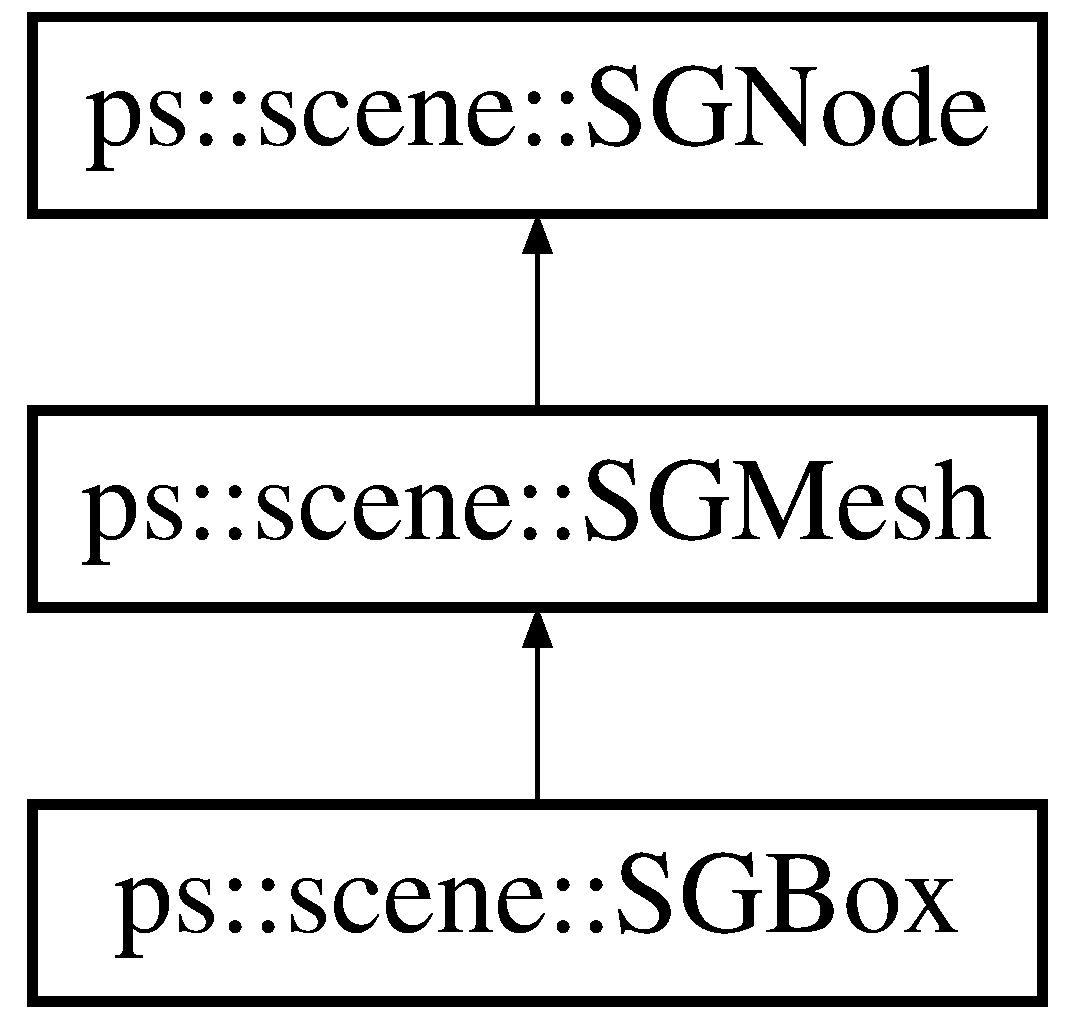
\includegraphics[height=3.000000cm]{classps_1_1scene_1_1SGBox}
\end{center}
\end{figure}
\subsection*{Public Member Functions}
\begin{DoxyCompactItemize}
\item 
\hypertarget{classps_1_1scene_1_1SGBox_afe50d22303e1a22efa4b438d85f76a30}{}{\bfseries S\+G\+Box} (const \hyperlink{classps_1_1base_1_1Vec3}{vec3f} \&lo, const \hyperlink{classps_1_1base_1_1Vec3}{vec3f} \&hi)\label{classps_1_1scene_1_1SGBox_afe50d22303e1a22efa4b438d85f76a30}

\item 
\hypertarget{classps_1_1scene_1_1SGBox_ae1093216bb21d691f689a9d463d8eaeb}{}void {\bfseries setup} (const \hyperlink{classps_1_1base_1_1Vec3}{vec3f} \&lo, const \hyperlink{classps_1_1base_1_1Vec3}{vec3f} \&hi)\label{classps_1_1scene_1_1SGBox_ae1093216bb21d691f689a9d463d8eaeb}

\item 
\hypertarget{classps_1_1scene_1_1SGBox_abd52c00d14ffa2f7ea6c679bf7df5583}{}void {\bfseries draw} ()\label{classps_1_1scene_1_1SGBox_abd52c00d14ffa2f7ea6c679bf7df5583}

\item 
\hypertarget{classps_1_1scene_1_1SGBox_a07a605e581e5740f5222461de12c3037}{}float {\bfseries width} () const \label{classps_1_1scene_1_1SGBox_a07a605e581e5740f5222461de12c3037}

\item 
\hypertarget{classps_1_1scene_1_1SGBox_af659d949ab269cf52ec68381b6402c25}{}float {\bfseries height} () const \label{classps_1_1scene_1_1SGBox_af659d949ab269cf52ec68381b6402c25}

\item 
\hypertarget{classps_1_1scene_1_1SGBox_acd985a0b9d6a403db97aaede05dcec90}{}float {\bfseries depth} () const \label{classps_1_1scene_1_1SGBox_acd985a0b9d6a403db97aaede05dcec90}

\item 
\hypertarget{classps_1_1scene_1_1SGBox_a77f528a487afba2e31491e4433e96301}{}\hyperlink{classps_1_1base_1_1Vec3}{vec3f} {\bfseries lo} () const \label{classps_1_1scene_1_1SGBox_a77f528a487afba2e31491e4433e96301}

\item 
\hypertarget{classps_1_1scene_1_1SGBox_a5a11a8afaa64e233cefbd9c12eb922ef}{}\hyperlink{classps_1_1base_1_1Vec3}{vec3f} {\bfseries hi} () const \label{classps_1_1scene_1_1SGBox_a5a11a8afaa64e233cefbd9c12eb922ef}

\end{DoxyCompactItemize}
\subsection*{Additional Inherited Members}


The documentation for this class was generated from the following files\+:\begin{DoxyCompactItemize}
\item 
/\+Users/pourya/\+Desktop/platform/repos/tetcutter/src/scene/sgbox.\+h\item 
/\+Users/pourya/\+Desktop/platform/repos/tetcutter/src/scene/sgbox.\+cpp\end{DoxyCompactItemize}

\hypertarget{classps_1_1scene_1_1SGEffect}{}\section{ps\+:\+:scene\+:\+:S\+G\+Effect Class Reference}
\label{classps_1_1scene_1_1SGEffect}\index{ps\+::scene\+::\+S\+G\+Effect@{ps\+::scene\+::\+S\+G\+Effect}}
Inheritance diagram for ps\+:\+:scene\+:\+:S\+G\+Effect\+:\begin{figure}[H]
\begin{center}
\leavevmode
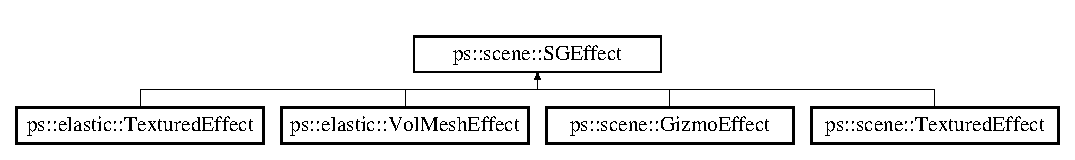
\includegraphics[height=1.707317cm]{classps_1_1scene_1_1SGEffect}
\end{center}
\end{figure}
\subsection*{Public Types}
\begin{DoxyCompactItemize}
\item 
\hypertarget{classps_1_1scene_1_1SGEffect_af8aa65adec9facbd6940d167509fc361}{}enum {\bfseries Effect\+Type} \{ {\bfseries et\+Material}, 
{\bfseries et\+Texture}, 
{\bfseries et\+Custom\+Shader}
 \}\label{classps_1_1scene_1_1SGEffect_af8aa65adec9facbd6940d167509fc361}

\end{DoxyCompactItemize}
\subsection*{Public Member Functions}
\begin{DoxyCompactItemize}
\item 
\hypertarget{classps_1_1scene_1_1SGEffect_a4ffe6c1802d21dbef4b2f8fff85c1897}{}{\bfseries S\+G\+Effect} (\hyperlink{classps_1_1opengl_1_1GLShader}{G\+L\+Shader} $\ast$s)\label{classps_1_1scene_1_1SGEffect_a4ffe6c1802d21dbef4b2f8fff85c1897}

\item 
\hypertarget{classps_1_1scene_1_1SGEffect_a912b62d95007fe4417ef0fb3b9a31733}{}virtual void {\bfseries bind} ()\label{classps_1_1scene_1_1SGEffect_a912b62d95007fe4417ef0fb3b9a31733}

\item 
\hypertarget{classps_1_1scene_1_1SGEffect_ac6dd6ec83a77843c4352955bdfa540eb}{}virtual void {\bfseries unbind} ()\label{classps_1_1scene_1_1SGEffect_ac6dd6ec83a77843c4352955bdfa540eb}

\item 
\hypertarget{classps_1_1scene_1_1SGEffect_a7a4fd2356132d434a6f1d0413bd59d15}{}\hyperlink{classps_1_1opengl_1_1GLShader}{G\+L\+Shader} $\ast$ {\bfseries shader} () const \label{classps_1_1scene_1_1SGEffect_a7a4fd2356132d434a6f1d0413bd59d15}

\item 
\hypertarget{classps_1_1scene_1_1SGEffect_abccb3ebbb2424f50c369077dcd46e73c}{}void {\bfseries set\+Shader} (\hyperlink{classps_1_1opengl_1_1GLShader}{G\+L\+Shader} $\ast$s)\label{classps_1_1scene_1_1SGEffect_abccb3ebbb2424f50c369077dcd46e73c}

\end{DoxyCompactItemize}
\subsection*{Protected Attributes}
\begin{DoxyCompactItemize}
\item 
\hypertarget{classps_1_1scene_1_1SGEffect_a763d22386f6b6bae55e4e808d9804738}{}\hyperlink{classps_1_1opengl_1_1GLShader}{G\+L\+Shader} $\ast$ {\bfseries m\+\_\+lp\+Shader}\label{classps_1_1scene_1_1SGEffect_a763d22386f6b6bae55e4e808d9804738}

\item 
\hypertarget{classps_1_1scene_1_1SGEffect_ae9f2cc9d8c543ae35661db926e84cc0a}{}Effect\+Type {\bfseries m\+\_\+etype}\label{classps_1_1scene_1_1SGEffect_ae9f2cc9d8c543ae35661db926e84cc0a}

\end{DoxyCompactItemize}


The documentation for this class was generated from the following files\+:\begin{DoxyCompactItemize}
\item 
/\+Users/pourya/\+Desktop/platform/repos/tetcutter/src/scene/sgeffect.\+h\item 
/\+Users/pourya/\+Desktop/platform/repos/tetcutter/src/scene/sgeffect.\+cpp\end{DoxyCompactItemize}

\hypertarget{classps_1_1scene_1_1SGEngine}{}\section{ps\+:\+:scene\+:\+:S\+G\+Engine Class Reference}
\label{classps_1_1scene_1_1SGEngine}\index{ps\+::scene\+::\+S\+G\+Engine@{ps\+::scene\+::\+S\+G\+Engine}}


{\ttfamily \#include $<$sgengine.\+h$>$}

Inheritance diagram for ps\+:\+:scene\+:\+:S\+G\+Engine\+:\begin{figure}[H]
\begin{center}
\leavevmode
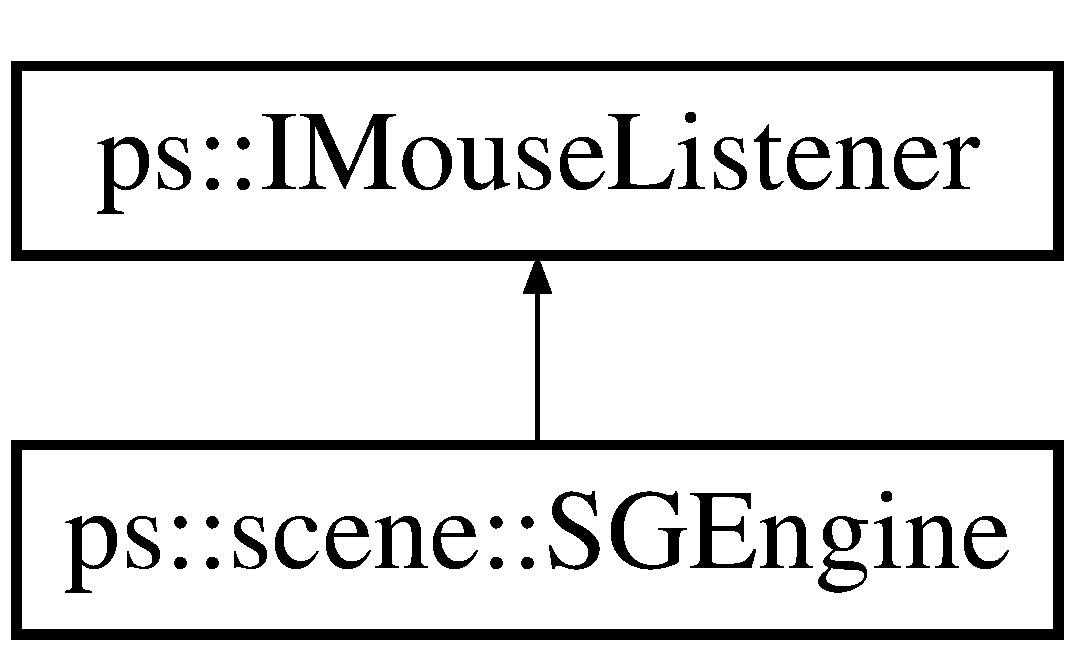
\includegraphics[height=2.000000cm]{classps_1_1scene_1_1SGEngine}
\end{center}
\end{figure}
\subsection*{Public Member Functions}
\begin{DoxyCompactItemize}
\item 
\hypertarget{classps_1_1scene_1_1SGEngine_a74eaee413e40470ba1e9bddedbfbc36c}{}void {\bfseries init} ()\label{classps_1_1scene_1_1SGEngine_a74eaee413e40470ba1e9bddedbfbc36c}

\item 
\hypertarget{classps_1_1scene_1_1SGEngine_ae4293eb87305b949db9cbbd09016d70f}{}void {\bfseries resize} (int w, int h)\label{classps_1_1scene_1_1SGEngine_ae4293eb87305b949db9cbbd09016d70f}

\item 
\hypertarget{classps_1_1scene_1_1SGEngine_a4a132d305999a5839af002611e30f2e5}{}void {\bfseries draw} ()\label{classps_1_1scene_1_1SGEngine_a4a132d305999a5839af002611e30f2e5}

\item 
\hypertarget{classps_1_1scene_1_1SGEngine_a570302efb3898600192d840ef90cbba4}{}void {\bfseries draw\+B\+Boxes} ()\label{classps_1_1scene_1_1SGEngine_a570302efb3898600192d840ef90cbba4}

\item 
\hypertarget{classps_1_1scene_1_1SGEngine_aafacce8f51ee18fb076f4b94a59488ed}{}void {\bfseries timestep} ()\label{classps_1_1scene_1_1SGEngine_aafacce8f51ee18fb076f4b94a59488ed}

\item 
\hypertarget{classps_1_1scene_1_1SGEngine_a504bbcd141b9f0fc3a474a4a27a75513}{}U32 {\bfseries add} (\hyperlink{classps_1_1scene_1_1SGNode}{S\+G\+Node} $\ast$a\+Node)\label{classps_1_1scene_1_1SGEngine_a504bbcd141b9f0fc3a474a4a27a75513}

\item 
\hypertarget{classps_1_1scene_1_1SGEngine_a66a380aa8a4534840ff2eb5da624d88f}{}U32 {\bfseries add\+Scene\+Box} (const \hyperlink{classps_1_1base_1_1AABB}{A\+A\+B\+B} \&box)\label{classps_1_1scene_1_1SGEngine_a66a380aa8a4534840ff2eb5da624d88f}

\item 
\hypertarget{classps_1_1scene_1_1SGEngine_aeba8022ce1742e97bfca50ce6d72198a}{}U32 {\bfseries add\+Floor} (int rows, int cols, float step=1.\+0f)\label{classps_1_1scene_1_1SGEngine_aeba8022ce1742e97bfca50ce6d72198a}

\item 
\hypertarget{classps_1_1scene_1_1SGEngine_a4d2fbb40e014948ebb223b8d7501f5e3}{}bool {\bfseries remove} (U32 index)\label{classps_1_1scene_1_1SGEngine_a4d2fbb40e014948ebb223b8d7501f5e3}

\item 
\hypertarget{classps_1_1scene_1_1SGEngine_aa00313d0c3a7104ad958f573e2d8470c}{}bool {\bfseries remove} (const string \&name)\label{classps_1_1scene_1_1SGEngine_aa00313d0c3a7104ad958f573e2d8470c}

\item 
\hypertarget{classps_1_1scene_1_1SGEngine_a1e754aa1bb9dcaf615f854872a24fdaf}{}bool {\bfseries remove} (const \hyperlink{classps_1_1scene_1_1SGNode}{S\+G\+Node} $\ast$pnode)\label{classps_1_1scene_1_1SGEngine_a1e754aa1bb9dcaf615f854872a24fdaf}

\item 
\hypertarget{classps_1_1scene_1_1SGEngine_a94ab3073aef12177cad62498495f7b47}{}U32 {\bfseries count} () const \label{classps_1_1scene_1_1SGEngine_a94ab3073aef12177cad62498495f7b47}

\item 
\hypertarget{classps_1_1scene_1_1SGEngine_a304ebc8af0faff31a74ec8a1b98143a4}{}\hyperlink{classps_1_1scene_1_1SGNode}{S\+G\+Node} $\ast$ {\bfseries get} (U32 index) const \label{classps_1_1scene_1_1SGEngine_a304ebc8af0faff31a74ec8a1b98143a4}

\item 
\hypertarget{classps_1_1scene_1_1SGEngine_ab88a5ba706d76698dd116b1cdf74b89f}{}\hyperlink{classps_1_1scene_1_1SGNode}{S\+G\+Node} $\ast$ {\bfseries get} (const char $\ast$name) const \label{classps_1_1scene_1_1SGEngine_ab88a5ba706d76698dd116b1cdf74b89f}

\item 
\hypertarget{classps_1_1scene_1_1SGEngine_ad550d5ebec257e0bb2ce8a8ef9517987}{}\hyperlink{classps_1_1scene_1_1SGNode}{S\+G\+Node} $\ast$ {\bfseries last} () const \label{classps_1_1scene_1_1SGEngine_ad550d5ebec257e0bb2ce8a8ef9517987}

\item 
\hypertarget{classps_1_1scene_1_1SGEngine_aee0da35acc575f4bd3ec7f7e51ad3d89}{}\hyperlink{classps_1_1base_1_1CopyStack}{Copy\+Stack}$<$ \hyperlink{classps_1_1base_1_1Matrix}{mat44f} $>$ \& {\bfseries stk\+Projection} ()\label{classps_1_1scene_1_1SGEngine_aee0da35acc575f4bd3ec7f7e51ad3d89}

\item 
\hypertarget{classps_1_1scene_1_1SGEngine_a1652a84acad74a46be809bde1fba6b71}{}\hyperlink{classps_1_1base_1_1CopyStack}{Copy\+Stack}$<$ \hyperlink{classps_1_1base_1_1Matrix}{mat44f} $>$ \& {\bfseries stk\+Model\+View} ()\label{classps_1_1scene_1_1SGEngine_a1652a84acad74a46be809bde1fba6b71}

\item 
\hypertarget{classps_1_1scene_1_1SGEngine_a503bcd135409aaeb34e81ae86989760b}{}\hyperlink{classps_1_1base_1_1Matrix}{mat44f} {\bfseries modelviewprojection} () const \label{classps_1_1scene_1_1SGEngine_a503bcd135409aaeb34e81ae86989760b}

\item 
\hypertarget{classps_1_1scene_1_1SGEngine_a4c75fdaec36509fb7514ce525fe51839}{}\hyperlink{classps_1_1scene_1_1ArcBallCamera}{Arc\+Ball\+Camera} \& {\bfseries camera} ()\label{classps_1_1scene_1_1SGEngine_a4c75fdaec36509fb7514ce525fe51839}

\item 
\hypertarget{classps_1_1scene_1_1SGEngine_a42d0aedf8ea474767800604c56461dd7}{}void {\bfseries mouse\+Press} (Mouse\+Button button, Mouse\+Button\+State state, int x, int y) override\label{classps_1_1scene_1_1SGEngine_a42d0aedf8ea474767800604c56461dd7}

\item 
\hypertarget{classps_1_1scene_1_1SGEngine_abfe59ca1d941e7e6d73af345169c74a5}{}void {\bfseries mouse\+Wheel} (Mouse\+Wheel\+Dir dir) override\label{classps_1_1scene_1_1SGEngine_abfe59ca1d941e7e6d73af345169c74a5}

\item 
\hypertarget{classps_1_1scene_1_1SGEngine_a0f9ab0012b7905f76d1e4a60e82524f6}{}void {\bfseries mouse\+Move} (int x, int y) override\label{classps_1_1scene_1_1SGEngine_a0f9ab0012b7905f76d1e4a60e82524f6}

\item 
\hypertarget{classps_1_1scene_1_1SGEngine_a75a0dacdcd15a90a0caa866e05999bf5}{}bool {\bfseries screen\+To\+World} (const \hyperlink{classps_1_1base_1_1Vec3}{vec3f} \&s, \hyperlink{classps_1_1base_1_1Vec3}{vec3f} \&w)\label{classps_1_1scene_1_1SGEngine_a75a0dacdcd15a90a0caa866e05999bf5}

\item 
\hypertarget{classps_1_1scene_1_1SGEngine_afbf3f9b67283bd90f1d087b1858ffdc8}{}\hyperlink{classps_1_1base_1_1Ray}{Ray} {\bfseries screen\+To\+World\+Ray} (int x, int y)\label{classps_1_1scene_1_1SGEngine_afbf3f9b67283bd90f1d087b1858ffdc8}

\item 
\hypertarget{classps_1_1scene_1_1SGEngine_a9b2ae67ded1e41e090557a317f917d87}{}\hyperlink{classps_1_1base_1_1Vec4}{vec4i} {\bfseries viewport} () const \label{classps_1_1scene_1_1SGEngine_a9b2ae67ded1e41e090557a317f917d87}

\item 
\hypertarget{classps_1_1scene_1_1SGEngine_af2bd2d9c29925ddbfce7b390b126d6e2}{}\hyperlink{classps_1_1scene_1_1SGHeaders}{S\+G\+Headers} $\ast$ {\bfseries headers} () const \label{classps_1_1scene_1_1SGEngine_af2bd2d9c29925ddbfce7b390b126d6e2}

\item 
\hypertarget{classps_1_1scene_1_1SGEngine_a98938ae4a3660d3779b91de5ac69dfb2}{}void {\bfseries update\+Camera\+Header} ()\label{classps_1_1scene_1_1SGEngine_a98938ae4a3660d3779b91de5ac69dfb2}

\item 
\hypertarget{classps_1_1scene_1_1SGEngine_a01ae618ecac6f3c8660eea0fb87a569f}{}int {\bfseries get\+Modifier} () const \label{classps_1_1scene_1_1SGEngine_a01ae618ecac6f3c8660eea0fb87a569f}

\item 
\hypertarget{classps_1_1scene_1_1SGEngine_a84a25b3c33e833a4ceb6fc9cca9647ce}{}void {\bfseries set\+Modifier} (int mod)\label{classps_1_1scene_1_1SGEngine_a84a25b3c33e833a4ceb6fc9cca9647ce}

\item 
\hypertarget{classps_1_1scene_1_1SGEngine_a2c8afcaa8a8db5f1e25906f6dca9527c}{}void {\bfseries update} ()\label{classps_1_1scene_1_1SGEngine_a2c8afcaa8a8db5f1e25906f6dca9527c}

\item 
\hypertarget{classps_1_1scene_1_1SGEngine_a1a6a9721de238a77e10c9d5d33d9f1b9}{}void {\bfseries print} (const char $\ast$switches=\char`\"{}-\/a\char`\"{}) const \label{classps_1_1scene_1_1SGEngine_a1a6a9721de238a77e10c9d5d33d9f1b9}

\item 
\hypertarget{classps_1_1scene_1_1SGEngine_a136af6df6e8d344a00568f06e86e2aca}{}bool {\bfseries read\+Config} (const \hyperlink{classps_1_1base_1_1CAString}{Ansi\+Str} \&str\+F\+P=\char`\"{}scene.\+ini\char`\"{})\label{classps_1_1scene_1_1SGEngine_a136af6df6e8d344a00568f06e86e2aca}

\item 
\hypertarget{classps_1_1scene_1_1SGEngine_aa23b0bd8826593e4e07f71561055d99c}{}bool {\bfseries write\+Config} (const \hyperlink{classps_1_1base_1_1CAString}{Ansi\+Str} \&str\+F\+P=\char`\"{}scene.\+ini\char`\"{})\label{classps_1_1scene_1_1SGEngine_aa23b0bd8826593e4e07f71561055d99c}

\end{DoxyCompactItemize}
\subsection*{Static Public Member Functions}
\begin{DoxyCompactItemize}
\item 
\hypertarget{classps_1_1scene_1_1SGEngine_afaf6d1ca62e58fbb80b3d0d6acd7d0f1}{}static \hyperlink{classps_1_1base_1_1CAString}{Ansi\+Str} {\bfseries gpu\+Info} ()\label{classps_1_1scene_1_1SGEngine_afaf6d1ca62e58fbb80b3d0d6acd7d0f1}

\end{DoxyCompactItemize}
\subsection*{Protected Member Functions}
\begin{DoxyCompactItemize}
\item 
\hypertarget{classps_1_1scene_1_1SGEngine_a4af4ea786996fff8b7e69a3272c4881e}{}void {\bfseries cleanup} ()\label{classps_1_1scene_1_1SGEngine_a4af4ea786996fff8b7e69a3272c4881e}

\end{DoxyCompactItemize}
\subsection*{Additional Inherited Members}


\subsection{Detailed Description}
Scene Graph 

The documentation for this class was generated from the following files\+:\begin{DoxyCompactItemize}
\item 
/\+Users/pourya/\+Desktop/platform/repos/tetcutter/src/scene/sgengine.\+h\item 
/\+Users/pourya/\+Desktop/platform/repos/tetcutter/src/scene/sgengine.\+cpp\end{DoxyCompactItemize}

\hypertarget{classps_1_1scene_1_1SGFloor}{}\section{ps\+:\+:scene\+:\+:S\+G\+Floor Class Reference}
\label{classps_1_1scene_1_1SGFloor}\index{ps\+::scene\+::\+S\+G\+Floor@{ps\+::scene\+::\+S\+G\+Floor}}
Inheritance diagram for ps\+:\+:scene\+:\+:S\+G\+Floor\+:\begin{figure}[H]
\begin{center}
\leavevmode
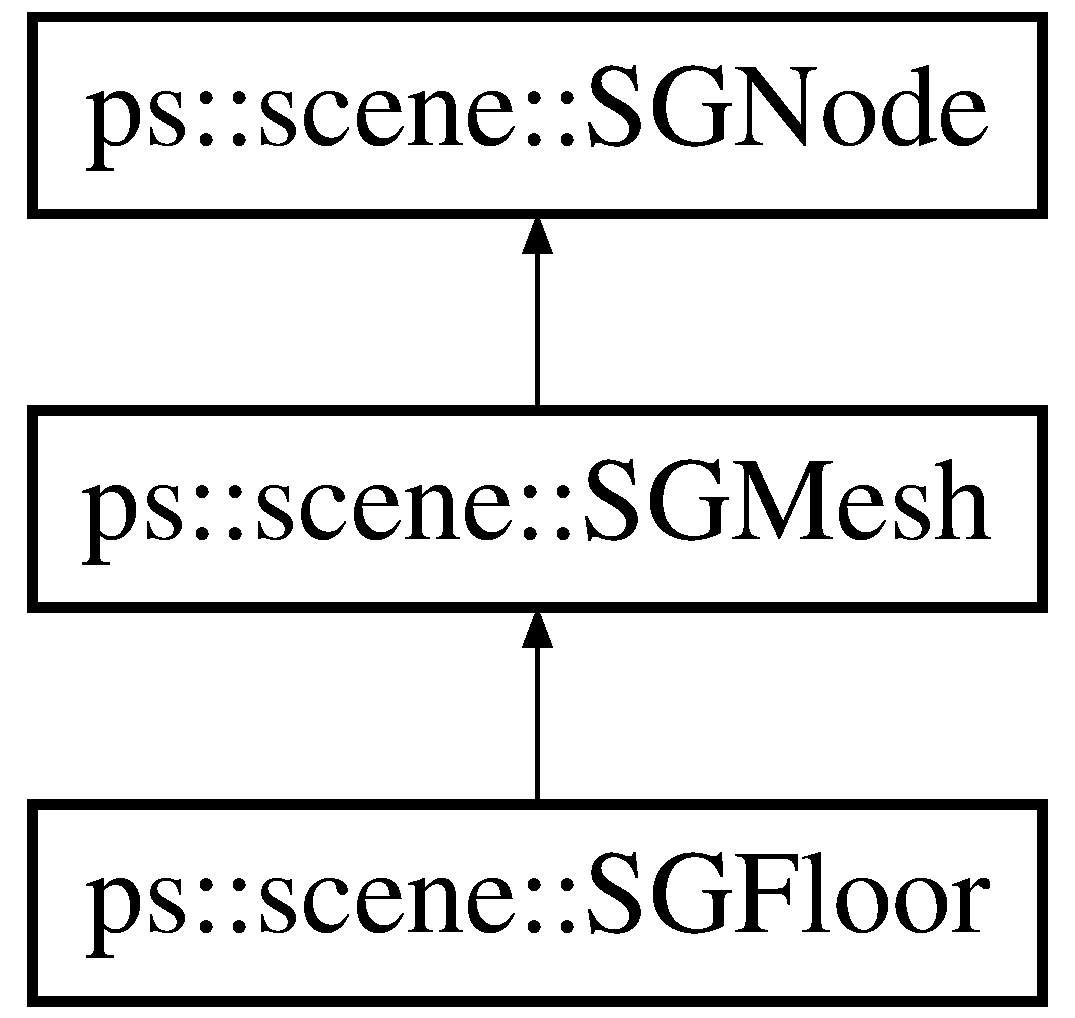
\includegraphics[height=3.000000cm]{classps_1_1scene_1_1SGFloor}
\end{center}
\end{figure}
\subsection*{Public Member Functions}
\begin{DoxyCompactItemize}
\item 
\hypertarget{classps_1_1scene_1_1SGFloor_a7bb0778ee29d7f18a1bb9f20c970f84a}{}{\bfseries S\+G\+Floor} (int rows=32, int cols=32, float step=1.\+0f)\label{classps_1_1scene_1_1SGFloor_a7bb0778ee29d7f18a1bb9f20c970f84a}

\item 
\hypertarget{classps_1_1scene_1_1SGFloor_a01e59616eb27367b8228084266fcf277}{}void {\bfseries draw} ()\label{classps_1_1scene_1_1SGFloor_a01e59616eb27367b8228084266fcf277}

\end{DoxyCompactItemize}
\subsection*{Additional Inherited Members}


The documentation for this class was generated from the following files\+:\begin{DoxyCompactItemize}
\item 
/\+Users/pourya/\+Desktop/platform/repos/tetcutter/src/scene/sgfloor.\+h\item 
/\+Users/pourya/\+Desktop/platform/repos/tetcutter/src/scene/sgfloor.\+cpp\end{DoxyCompactItemize}

\hypertarget{classps_1_1scene_1_1SGHeaders}{}\section{ps\+:\+:scene\+:\+:S\+G\+Headers Class Reference}
\label{classps_1_1scene_1_1SGHeaders}\index{ps\+::scene\+::\+S\+G\+Headers@{ps\+::scene\+::\+S\+G\+Headers}}
Inheritance diagram for ps\+:\+:scene\+:\+:S\+G\+Headers\+:\begin{figure}[H]
\begin{center}
\leavevmode
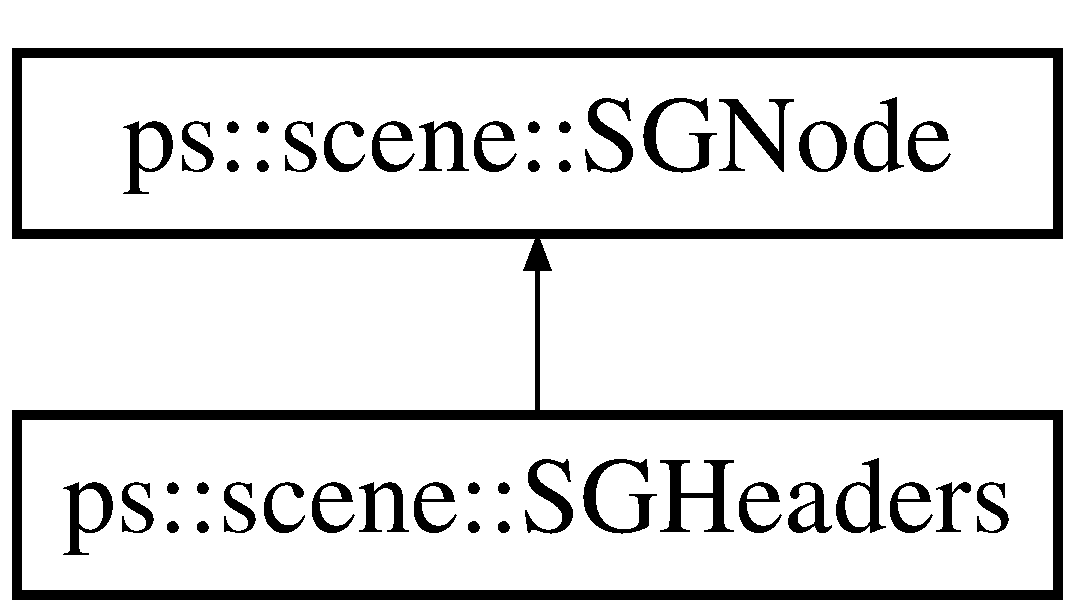
\includegraphics[height=2.000000cm]{classps_1_1scene_1_1SGHeaders}
\end{center}
\end{figure}
\subsection*{Public Member Functions}
\begin{DoxyCompactItemize}
\item 
\hypertarget{classps_1_1scene_1_1SGHeaders_a6dcebb075fefd4209dd6b059a543cb4f}{}void {\bfseries cleanup} ()\label{classps_1_1scene_1_1SGHeaders_a6dcebb075fefd4209dd6b059a543cb4f}

\item 
\hypertarget{classps_1_1scene_1_1SGHeaders_ac39e5dab01a381280d214b717bcb8b46}{}void {\bfseries draw} ()\label{classps_1_1scene_1_1SGHeaders_ac39e5dab01a381280d214b717bcb8b46}

\item 
\hypertarget{classps_1_1scene_1_1SGHeaders_ad362df2d7ee0e2cf20da258a3e69001c}{}int {\bfseries add\+Header\+Line} (const \hyperlink{classps_1_1base_1_1CAString}{Ansi\+Str} \&title, const \hyperlink{classps_1_1base_1_1CAString}{Ansi\+Str} \&str\+Info)\label{classps_1_1scene_1_1SGHeaders_ad362df2d7ee0e2cf20da258a3e69001c}

\item 
\hypertarget{classps_1_1scene_1_1SGHeaders_a51e502325499e2e4d413738c49c44b20}{}int {\bfseries get\+Header\+Id} (const char $\ast$title)\label{classps_1_1scene_1_1SGHeaders_a51e502325499e2e4d413738c49c44b20}

\item 
\hypertarget{classps_1_1scene_1_1SGHeaders_a433dc5477dc75f2028705c4d9029157c}{}bool {\bfseries remove\+Header\+Line} (const char $\ast$title)\label{classps_1_1scene_1_1SGHeaders_a433dc5477dc75f2028705c4d9029157c}

\item 
\hypertarget{classps_1_1scene_1_1SGHeaders_ad6c9f0fc6527becb9129d8623e4539bd}{}void {\bfseries remove\+All\+Headers} ()\label{classps_1_1scene_1_1SGHeaders_ad6c9f0fc6527becb9129d8623e4539bd}

\item 
\hypertarget{classps_1_1scene_1_1SGHeaders_a4320104f16e3c04228ce57fd5a76cf25}{}bool {\bfseries update\+Header\+Line} (int id, const \hyperlink{classps_1_1base_1_1CAString}{Ansi\+Str} \&str\+Info)\label{classps_1_1scene_1_1SGHeaders_a4320104f16e3c04228ce57fd5a76cf25}

\item 
\hypertarget{classps_1_1scene_1_1SGHeaders_a5eda7e8c04676c5b1cff7fbef3fc35e0}{}bool {\bfseries update\+Header\+Line} (const \hyperlink{classps_1_1base_1_1CAString}{Ansi\+Str} \&title, const \hyperlink{classps_1_1base_1_1CAString}{Ansi\+Str} \&str\+Info)\label{classps_1_1scene_1_1SGHeaders_a5eda7e8c04676c5b1cff7fbef3fc35e0}

\item 
\hypertarget{classps_1_1scene_1_1SGHeaders_a61ad34f586ce5b5522fdc2beda11c6a3}{}bool {\bfseries is\+Valid\+I\+D} (bool id)\label{classps_1_1scene_1_1SGHeaders_a61ad34f586ce5b5522fdc2beda11c6a3}

\end{DoxyCompactItemize}
\subsection*{Static Public Member Functions}
\begin{DoxyCompactItemize}
\item 
\hypertarget{classps_1_1scene_1_1SGHeaders_a512b8471d188fa4e8018f166ffb989ef}{}static void {\bfseries Draw\+Text} (const char $\ast$chr\+Text, int x, int y)\label{classps_1_1scene_1_1SGHeaders_a512b8471d188fa4e8018f166ffb989ef}

\end{DoxyCompactItemize}
\subsection*{Protected Attributes}
\begin{DoxyCompactItemize}
\item 
\hypertarget{classps_1_1scene_1_1SGHeaders_afc589b819662a7fdb8ac0045c71e3d89}{}std\+::vector$<$ \hyperlink{classps_1_1base_1_1CAString}{Ansi\+Str} $>$ {\bfseries m\+\_\+v\+Headers}\label{classps_1_1scene_1_1SGHeaders_afc589b819662a7fdb8ac0045c71e3d89}

\item 
\hypertarget{classps_1_1scene_1_1SGHeaders_a496d83efe2ac71f174ab1068a88e61fe}{}\hyperlink{classps_1_1FastAccessNamedResource}{Fast\+Access\+Named\+Resource}$<$ int, \hyperlink{structps_1_1TypeValue}{Type\+Value}, \hyperlink{structps_1_1InsertRemoveNoop}{Insert\+Remove\+Noop}, \hyperlink{structps_1_1Logging}{Logging}, false $>$ {\bfseries m\+\_\+hash\+Headers}\label{classps_1_1scene_1_1SGHeaders_a496d83efe2ac71f174ab1068a88e61fe}

\end{DoxyCompactItemize}


The documentation for this class was generated from the following files\+:\begin{DoxyCompactItemize}
\item 
/\+Users/pourya/\+Desktop/platform/repos/tetcutter/src/scene/sgheaders.\+h\item 
/\+Users/pourya/\+Desktop/platform/repos/tetcutter/src/scene/sgheaders.\+cpp\end{DoxyCompactItemize}

\hypertarget{classps_1_1scene_1_1SGMesh}{}\section{ps\+:\+:scene\+:\+:S\+G\+Mesh Class Reference}
\label{classps_1_1scene_1_1SGMesh}\index{ps\+::scene\+::\+S\+G\+Mesh@{ps\+::scene\+::\+S\+G\+Mesh}}
Inheritance diagram for ps\+:\+:scene\+:\+:S\+G\+Mesh\+:\begin{figure}[H]
\begin{center}
\leavevmode
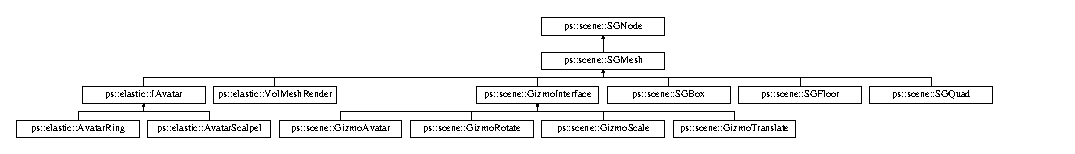
\includegraphics[height=1.627907cm]{classps_1_1scene_1_1SGMesh}
\end{center}
\end{figure}
\subsection*{Public Member Functions}
\begin{DoxyCompactItemize}
\item 
\hypertarget{classps_1_1scene_1_1SGMesh_ab9f55878b86063412f7998000d118430}{}{\bfseries S\+G\+Mesh} (const \hyperlink{classps_1_1scene_1_1Geometry}{Geometry} \&g)\label{classps_1_1scene_1_1SGMesh_ab9f55878b86063412f7998000d118430}

\item 
\hypertarget{classps_1_1scene_1_1SGMesh_aaa3f47f4132a037d6149aaaec70403ad}{}{\bfseries S\+G\+Mesh} (const \hyperlink{classps_1_1base_1_1CAString}{Ansi\+Str} \&str\+File\+Path)\label{classps_1_1scene_1_1SGMesh_aaa3f47f4132a037d6149aaaec70403ad}

\item 
\hypertarget{classps_1_1scene_1_1SGMesh_a989c881261d9eb732ed550e86b9e434f}{}void {\bfseries setup} (const \hyperlink{classps_1_1scene_1_1Geometry}{Geometry} \&g)\label{classps_1_1scene_1_1SGMesh_a989c881261d9eb732ed550e86b9e434f}

\item 
\hypertarget{classps_1_1scene_1_1SGMesh_ac17391a0c735b5978269cf461aa2bfee}{}virtual void {\bfseries draw} ()\label{classps_1_1scene_1_1SGMesh_ac17391a0c735b5978269cf461aa2bfee}

\item 
\hypertarget{classps_1_1scene_1_1SGMesh_a11b6a3946977d278ae2ddf722f7ce5d5}{}virtual void {\bfseries draw\+No\+Effect} ()\label{classps_1_1scene_1_1SGMesh_a11b6a3946977d278ae2ddf722f7ce5d5}

\item 
\hypertarget{classps_1_1scene_1_1SGMesh_af847f0e5e010d8df3656a40e733388ac}{}\hyperlink{classps_1_1opengl_1_1GLMesh}{G\+L\+Mesh} \& {\bfseries glmesh} ()\label{classps_1_1scene_1_1SGMesh_af847f0e5e010d8df3656a40e733388ac}

\item 
\hypertarget{classps_1_1scene_1_1SGMesh_a30627b03bd6e3052d4dfb33d6c8f33df}{}const \hyperlink{classps_1_1opengl_1_1GLMesh}{G\+L\+Mesh} \& {\bfseries const\+\_\+glmesh} () const \label{classps_1_1scene_1_1SGMesh_a30627b03bd6e3052d4dfb33d6c8f33df}

\end{DoxyCompactItemize}
\subsection*{Protected Attributes}
\begin{DoxyCompactItemize}
\item 
\hypertarget{classps_1_1scene_1_1SGMesh_ad1d4d7b11d99bcc4d6dee106191fb0cf}{}\hyperlink{classps_1_1opengl_1_1GLMesh}{G\+L\+Mesh} {\bfseries m\+\_\+meshbuffer}\label{classps_1_1scene_1_1SGMesh_ad1d4d7b11d99bcc4d6dee106191fb0cf}

\end{DoxyCompactItemize}


The documentation for this class was generated from the following files\+:\begin{DoxyCompactItemize}
\item 
/\+Users/pourya/\+Desktop/platform/repos/tetcutter/src/scene/sgmesh.\+h\item 
/\+Users/pourya/\+Desktop/platform/repos/tetcutter/src/scene/sgmesh.\+cpp\end{DoxyCompactItemize}

\hypertarget{classps_1_1scene_1_1SGNode}{}\section{ps\+:\+:scene\+:\+:S\+G\+Node Class Reference}
\label{classps_1_1scene_1_1SGNode}\index{ps\+::scene\+::\+S\+G\+Node@{ps\+::scene\+::\+S\+G\+Node}}


The Scene\+Node class is an element in the scenegraph can have effect and transformation associated with.  




{\ttfamily \#include $<$sgnode.\+h$>$}

Inheritance diagram for ps\+:\+:scene\+:\+:S\+G\+Node\+:\begin{figure}[H]
\begin{center}
\leavevmode
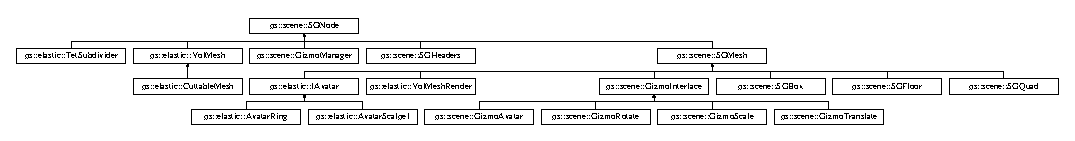
\includegraphics[height=1.447028cm]{classps_1_1scene_1_1SGNode}
\end{center}
\end{figure}
\subsection*{Public Member Functions}
\begin{DoxyCompactItemize}
\item 
\hypertarget{classps_1_1scene_1_1SGNode_a0d163b007bfe81737ecca9136817d0ee}{}{\bfseries S\+G\+Node} (const string \&name, bool visible=true)\label{classps_1_1scene_1_1SGNode_a0d163b007bfe81737ecca9136817d0ee}

\item 
\hypertarget{classps_1_1scene_1_1SGNode_a6e75d7d271c4a97084561a01b1861061}{}virtual void {\bfseries draw} ()=0\label{classps_1_1scene_1_1SGNode_a6e75d7d271c4a97084561a01b1861061}

\item 
\hypertarget{classps_1_1scene_1_1SGNode_a0d3ba806dc24ec372352f72b3eb1cd1d}{}virtual void {\bfseries draw\+B\+Box} () const \label{classps_1_1scene_1_1SGNode_a0d3ba806dc24ec372352f72b3eb1cd1d}

\item 
\hypertarget{classps_1_1scene_1_1SGNode_a098937b04b4eb9ca87e592406c103c5b}{}virtual void {\bfseries timestep} ()\label{classps_1_1scene_1_1SGNode_a098937b04b4eb9ca87e592406c103c5b}

\item 
\hypertarget{classps_1_1scene_1_1SGNode_a77853b8d93bc3aa8d38ef2ca74cb953f}{}void {\bfseries set\+A\+A\+B\+B} (const \hyperlink{classps_1_1base_1_1AABB}{A\+A\+B\+B} \&box)\label{classps_1_1scene_1_1SGNode_a77853b8d93bc3aa8d38ef2ca74cb953f}

\item 
\hypertarget{classps_1_1scene_1_1SGNode_ab400b91c61a9f06439fa5681f9184736}{}virtual \hyperlink{classps_1_1base_1_1AABB}{A\+A\+B\+B} {\bfseries aabb} () const \label{classps_1_1scene_1_1SGNode_ab400b91c61a9f06439fa5681f9184736}

\item 
\hypertarget{classps_1_1scene_1_1SGNode_af5efe8ab82d5a51cb5175f8bb56a5a15}{}virtual int {\bfseries intersect} (const \hyperlink{classps_1_1base_1_1Ray}{Ray} \&r)\label{classps_1_1scene_1_1SGNode_af5efe8ab82d5a51cb5175f8bb56a5a15}

\item 
\hypertarget{classps_1_1scene_1_1SGNode_a778d3daa84907e37f48e600fb0cc5301}{}string {\bfseries name} () const \label{classps_1_1scene_1_1SGNode_a778d3daa84907e37f48e600fb0cc5301}

\item 
\hypertarget{classps_1_1scene_1_1SGNode_a663dff07124b0ab20870a33b4c393e6e}{}void {\bfseries set\+Name} (const string \&name)\label{classps_1_1scene_1_1SGNode_a663dff07124b0ab20870a33b4c393e6e}

\item 
\hypertarget{classps_1_1scene_1_1SGNode_a313af13aad934c6f61c05c0cc76f0514}{}bool {\bfseries is\+Visible} () const \label{classps_1_1scene_1_1SGNode_a313af13aad934c6f61c05c0cc76f0514}

\item 
\hypertarget{classps_1_1scene_1_1SGNode_a729e7c8652b68af6a1daa9bc7c49461c}{}void {\bfseries set\+Visible} (bool visible)\label{classps_1_1scene_1_1SGNode_a729e7c8652b68af6a1daa9bc7c49461c}

\item 
\hypertarget{classps_1_1scene_1_1SGNode_ad887fe4547b56e8a18664e6755ee6460}{}bool {\bfseries is\+Animate} () const \label{classps_1_1scene_1_1SGNode_ad887fe4547b56e8a18664e6755ee6460}

\item 
\hypertarget{classps_1_1scene_1_1SGNode_ab7556b1a929ec8430af765570df35b86}{}void {\bfseries set\+Animate} (bool animate)\label{classps_1_1scene_1_1SGNode_ab7556b1a929ec8430af765570df35b86}

\item 
\hypertarget{classps_1_1scene_1_1SGNode_a90d373c716ad744b3314741383df156d}{}bool {\bfseries is\+Selected} () const \label{classps_1_1scene_1_1SGNode_a90d373c716ad744b3314741383df156d}

\item 
\hypertarget{classps_1_1scene_1_1SGNode_a646ecc45f3317fcb8327f4d6879f00d4}{}void {\bfseries set\+Selected} (bool selected)\label{classps_1_1scene_1_1SGNode_a646ecc45f3317fcb8327f4d6879f00d4}

\item 
\hypertarget{classps_1_1scene_1_1SGNode_a37b24105ff1343f7bd4a3cbf803dd06e}{}Smart\+Ptr\+S\+G\+Effect {\bfseries effect} () const \label{classps_1_1scene_1_1SGNode_a37b24105ff1343f7bd4a3cbf803dd06e}

\item 
\hypertarget{classps_1_1scene_1_1SGNode_a68ca301dfa5ab6d390ca462fbba605e8}{}void {\bfseries set\+Effect} (const Smart\+Ptr\+S\+G\+Effect \&sp\+Effect)\label{classps_1_1scene_1_1SGNode_a68ca301dfa5ab6d390ca462fbba605e8}

\item 
\hypertarget{classps_1_1scene_1_1SGNode_ab0423fcc76b2dd09bb63c841961660b2}{}Smart\+Ptr\+S\+G\+Transform {\bfseries transform} () const \label{classps_1_1scene_1_1SGNode_ab0423fcc76b2dd09bb63c841961660b2}

\item 
\hypertarget{classps_1_1scene_1_1SGNode_add7bf24c519c2d8bacdb2d1e845091b9}{}void {\bfseries set\+Transform} (const Smart\+Ptr\+S\+G\+Transform \&rhs)\label{classps_1_1scene_1_1SGNode_add7bf24c519c2d8bacdb2d1e845091b9}

\item 
\hypertarget{classps_1_1scene_1_1SGNode_ae6e30d330b583ea8d896b684f2250ea3}{}void {\bfseries reset\+Transform} ()\label{classps_1_1scene_1_1SGNode_ae6e30d330b583ea8d896b684f2250ea3}

\item 
\hypertarget{classps_1_1scene_1_1SGNode_abe81619307d1ad4a16e6c3c629e114b8}{}bool {\bfseries read} ()\label{classps_1_1scene_1_1SGNode_abe81619307d1ad4a16e6c3c629e114b8}

\item 
\hypertarget{classps_1_1scene_1_1SGNode_a3f4c5597ed44a634681a871d267a36f7}{}bool {\bfseries write} ()\label{classps_1_1scene_1_1SGNode_a3f4c5597ed44a634681a871d267a36f7}

\end{DoxyCompactItemize}
\subsection*{Protected Attributes}
\begin{DoxyCompactItemize}
\item 
\hypertarget{classps_1_1scene_1_1SGNode_a6f34ae5f7e3e364a097f38052e312d14}{}\hyperlink{classps_1_1base_1_1AABB}{A\+A\+B\+B} {\bfseries m\+\_\+aabb}\label{classps_1_1scene_1_1SGNode_a6f34ae5f7e3e364a097f38052e312d14}

\item 
\hypertarget{classps_1_1scene_1_1SGNode_ab138751ca18f8c4abbd659131510987f}{}string {\bfseries m\+\_\+name}\label{classps_1_1scene_1_1SGNode_ab138751ca18f8c4abbd659131510987f}

\item 
\hypertarget{classps_1_1scene_1_1SGNode_acf56b812a560048ac80c5b8af5e83554}{}bool {\bfseries m\+\_\+visible}\label{classps_1_1scene_1_1SGNode_acf56b812a560048ac80c5b8af5e83554}

\item 
\hypertarget{classps_1_1scene_1_1SGNode_a2ce4ff6c162645183409a6c9a7130c00}{}bool {\bfseries m\+\_\+animate}\label{classps_1_1scene_1_1SGNode_a2ce4ff6c162645183409a6c9a7130c00}

\item 
\hypertarget{classps_1_1scene_1_1SGNode_a6596ed2743cf693a8707ff61a03203e8}{}bool {\bfseries m\+\_\+selected}\label{classps_1_1scene_1_1SGNode_a6596ed2743cf693a8707ff61a03203e8}

\item 
\hypertarget{classps_1_1scene_1_1SGNode_a4a7f4fc053955264adcafe62903ae94e}{}std\+::shared\+\_\+ptr$<$ \hyperlink{classps_1_1scene_1_1SGEffect}{S\+G\+Effect} $>$ {\bfseries m\+\_\+sp\+Effect}\label{classps_1_1scene_1_1SGNode_a4a7f4fc053955264adcafe62903ae94e}

\item 
\hypertarget{classps_1_1scene_1_1SGNode_ac3ee6a415828679621309e0a8db3f0e8}{}std\+::shared\+\_\+ptr$<$ \hyperlink{classps_1_1scene_1_1SGTransform}{S\+G\+Transform} $>$ {\bfseries m\+\_\+sp\+Transform}\label{classps_1_1scene_1_1SGNode_ac3ee6a415828679621309e0a8db3f0e8}

\end{DoxyCompactItemize}


\subsection{Detailed Description}
The Scene\+Node class is an element in the scenegraph can have effect and transformation associated with. 

The documentation for this class was generated from the following files\+:\begin{DoxyCompactItemize}
\item 
/\+Users/pourya/\+Desktop/platform/repos/tetcutter/src/scene/sgnode.\+h\item 
/\+Users/pourya/\+Desktop/platform/repos/tetcutter/src/scene/sgnode.\+cpp\end{DoxyCompactItemize}

\hypertarget{classps_1_1scene_1_1SGQuad}{}\section{ps\+:\+:scene\+:\+:S\+G\+Quad Class Reference}
\label{classps_1_1scene_1_1SGQuad}\index{ps\+::scene\+::\+S\+G\+Quad@{ps\+::scene\+::\+S\+G\+Quad}}
Inheritance diagram for ps\+:\+:scene\+:\+:S\+G\+Quad\+:\begin{figure}[H]
\begin{center}
\leavevmode
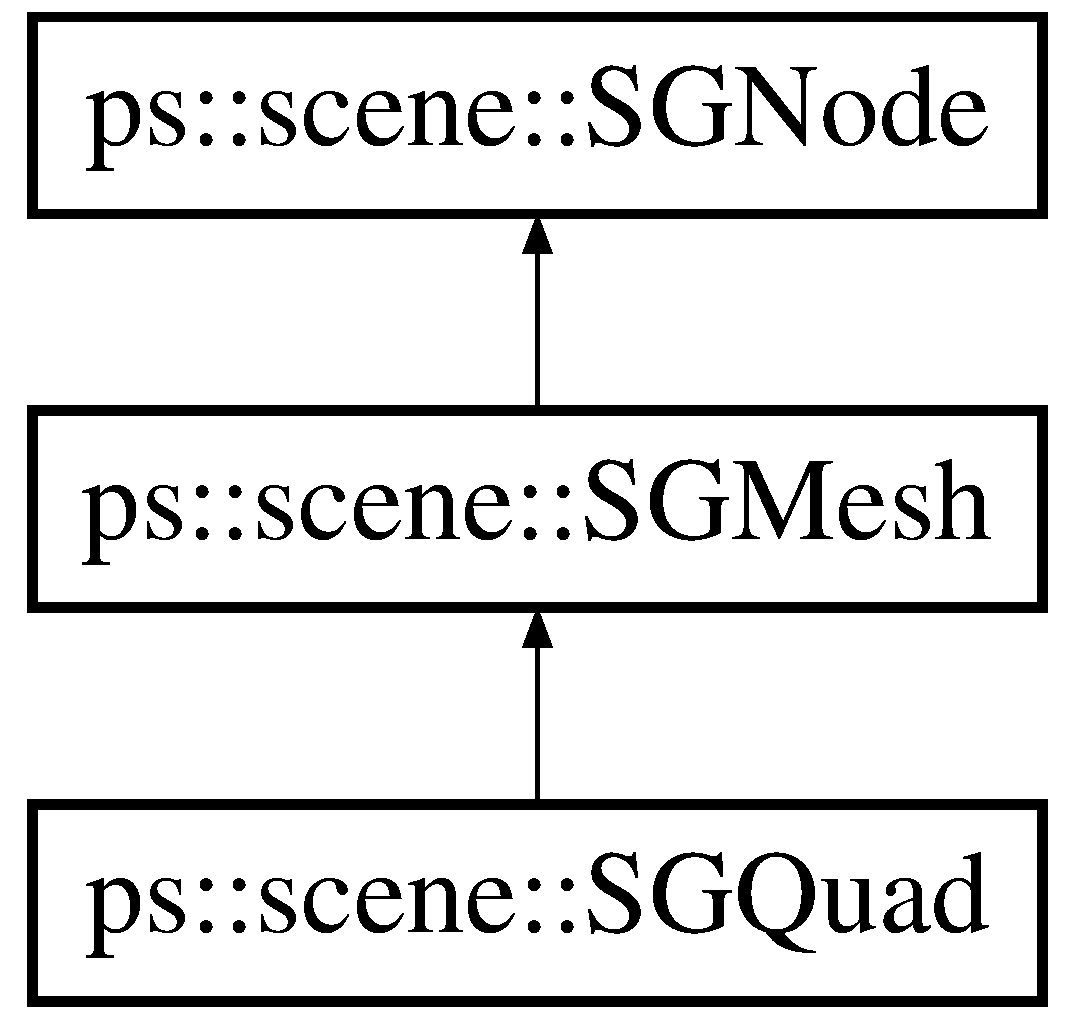
\includegraphics[height=3.000000cm]{classps_1_1scene_1_1SGQuad}
\end{center}
\end{figure}
\subsection*{Public Member Functions}
\begin{DoxyCompactItemize}
\item 
\hypertarget{classps_1_1scene_1_1SGQuad_a3fb9a5a10d9301c9fa46e7b401adec98}{}{\bfseries S\+G\+Quad} (float w, float h, \hyperlink{classps_1_1opengl_1_1GLTexture}{G\+L\+Texture} $\ast$a\+Tex=N\+U\+L\+L)\label{classps_1_1scene_1_1SGQuad_a3fb9a5a10d9301c9fa46e7b401adec98}

\item 
\hypertarget{classps_1_1scene_1_1SGQuad_abd2907cfb1ed9178ac0e700c18c24fd2}{}virtual void {\bfseries draw} ()\label{classps_1_1scene_1_1SGQuad_abd2907cfb1ed9178ac0e700c18c24fd2}

\item 
\hypertarget{classps_1_1scene_1_1SGQuad_ad02ccfed33193a153403f97c14063ea3}{}void {\bfseries set\+Texture} (\hyperlink{classps_1_1opengl_1_1GLTexture}{G\+L\+Texture} $\ast$lp\+Tex)\label{classps_1_1scene_1_1SGQuad_ad02ccfed33193a153403f97c14063ea3}

\end{DoxyCompactItemize}
\subsection*{Protected Member Functions}
\begin{DoxyCompactItemize}
\item 
\hypertarget{classps_1_1scene_1_1SGQuad_acab2a4abc50a608f5fae42d1da9b3f34}{}void {\bfseries setup} (float w, float h)\label{classps_1_1scene_1_1SGQuad_acab2a4abc50a608f5fae42d1da9b3f34}

\end{DoxyCompactItemize}
\subsection*{Protected Attributes}
\begin{DoxyCompactItemize}
\item 
\hypertarget{classps_1_1scene_1_1SGQuad_a66b716e1fb9c9ce66a64c20db650860c}{}\hyperlink{classps_1_1opengl_1_1GLTexture}{G\+L\+Texture} $\ast$ {\bfseries m\+\_\+lp\+Tex}\label{classps_1_1scene_1_1SGQuad_a66b716e1fb9c9ce66a64c20db650860c}

\end{DoxyCompactItemize}


The documentation for this class was generated from the following files\+:\begin{DoxyCompactItemize}
\item 
/\+Users/pourya/\+Desktop/platform/repos/tetcutter/src/scene/sgquad.\+h\item 
/\+Users/pourya/\+Desktop/platform/repos/tetcutter/src/scene/sgquad.\+cpp\end{DoxyCompactItemize}

\hypertarget{classps_1_1scene_1_1SGTransform}{}\section{ps\+:\+:scene\+:\+:S\+G\+Transform Class Reference}
\label{classps_1_1scene_1_1SGTransform}\index{ps\+::scene\+::\+S\+G\+Transform@{ps\+::scene\+::\+S\+G\+Transform}}


{\ttfamily \#include $<$sgtransform.\+h$>$}

\subsection*{Public Member Functions}
\begin{DoxyCompactItemize}
\item 
\hypertarget{classps_1_1scene_1_1SGTransform_afaf5a87138dabd0aacac5545bfbcd2d2}{}{\bfseries S\+G\+Transform} (bool b\+Auto\+Update\+Backward=false)\label{classps_1_1scene_1_1SGTransform_afaf5a87138dabd0aacac5545bfbcd2d2}

\item 
\hypertarget{classps_1_1scene_1_1SGTransform_a7726860818c1d0f69ffae1bf198a82f7}{}{\bfseries S\+G\+Transform} (const \hyperlink{classps_1_1scene_1_1SGTransform}{S\+G\+Transform} \&other)\label{classps_1_1scene_1_1SGTransform_a7726860818c1d0f69ffae1bf198a82f7}

\item 
\hypertarget{classps_1_1scene_1_1SGTransform_a8d45f9b4735efffbd076d40c79a78e7a}{}void {\bfseries copy\+From} (const \hyperlink{classps_1_1scene_1_1SGTransform}{S\+G\+Transform} \&other)\label{classps_1_1scene_1_1SGTransform_a8d45f9b4735efffbd076d40c79a78e7a}

\item 
\hypertarget{classps_1_1scene_1_1SGTransform_adb066652059d4045d722fc6f61c6b87a}{}void {\bfseries scale} (const \hyperlink{classps_1_1base_1_1Vec3}{vec3f} \&delta)\label{classps_1_1scene_1_1SGTransform_adb066652059d4045d722fc6f61c6b87a}

\item 
\hypertarget{classps_1_1scene_1_1SGTransform_aebad2680e9d8a356231721515e865201}{}void {\bfseries scale} (float sfactor)\label{classps_1_1scene_1_1SGTransform_aebad2680e9d8a356231721515e865201}

\item 
\hypertarget{classps_1_1scene_1_1SGTransform_a0875af7b739cec704217e420cfcf502d}{}void {\bfseries rotate} (const \hyperlink{classps_1_1base_1_1Quaternion}{quat} \&q)\label{classps_1_1scene_1_1SGTransform_a0875af7b739cec704217e420cfcf502d}

\item 
\hypertarget{classps_1_1scene_1_1SGTransform_a4c7191b65002f91c637627a76310b9e3}{}void {\bfseries rotate} (const \hyperlink{classps_1_1base_1_1Vec3}{vec3f} \&axis, float deg)\label{classps_1_1scene_1_1SGTransform_a4c7191b65002f91c637627a76310b9e3}

\item 
\hypertarget{classps_1_1scene_1_1SGTransform_a9798fa4ae63a127867fab9dd5b3ad366}{}void {\bfseries translate} (const \hyperlink{classps_1_1base_1_1Vec3}{vec3f} \&delta)\label{classps_1_1scene_1_1SGTransform_a9798fa4ae63a127867fab9dd5b3ad366}

\item 
\hypertarget{classps_1_1scene_1_1SGTransform_a16fbb4c47353c9f40a096bca94b2d1c7}{}\hyperlink{classps_1_1base_1_1Vec3}{vec3f} {\bfseries get\+Scale} () const \label{classps_1_1scene_1_1SGTransform_a16fbb4c47353c9f40a096bca94b2d1c7}

\item 
\hypertarget{classps_1_1scene_1_1SGTransform_a4a5a7c081d6f750bb197422ff9239d77}{}\hyperlink{classps_1_1base_1_1Vec3}{vec3f} {\bfseries get\+Translate} () const \label{classps_1_1scene_1_1SGTransform_a4a5a7c081d6f750bb197422ff9239d77}

\item 
\hypertarget{classps_1_1scene_1_1SGTransform_a3f1c5e9fb98c99b3f562664a1a0e6850}{}\hyperlink{classps_1_1base_1_1Quaternion}{quatf} {\bfseries get\+Rotate} () const \label{classps_1_1scene_1_1SGTransform_a3f1c5e9fb98c99b3f562664a1a0e6850}

\item 
\hypertarget{classps_1_1scene_1_1SGTransform_a1cd22a1ba9d5bb3b852e78ecb02a460a}{}void {\bfseries set\+Scale} (const \hyperlink{classps_1_1base_1_1Vec3}{vec3f} \&s)\label{classps_1_1scene_1_1SGTransform_a1cd22a1ba9d5bb3b852e78ecb02a460a}

\item 
\hypertarget{classps_1_1scene_1_1SGTransform_a6cfac3d485986943a67934a526a267ff}{}void {\bfseries set\+Rotate} (const \hyperlink{classps_1_1base_1_1Quaternion}{quat} \&r)\label{classps_1_1scene_1_1SGTransform_a6cfac3d485986943a67934a526a267ff}

\item 
\hypertarget{classps_1_1scene_1_1SGTransform_af0eda3002b631332a12552bbf9a9281f}{}void {\bfseries set\+Translate} (const \hyperlink{classps_1_1base_1_1Vec3}{vec3f} \&t)\label{classps_1_1scene_1_1SGTransform_af0eda3002b631332a12552bbf9a9281f}

\item 
\hypertarget{classps_1_1scene_1_1SGTransform_af1a72953319100d337d921b514a781c6}{}void {\bfseries reset} ()\label{classps_1_1scene_1_1SGTransform_af1a72953319100d337d921b514a781c6}

\item 
\hypertarget{classps_1_1scene_1_1SGTransform_a06cdc843c3586f5a868168240e9e81e9}{}void {\bfseries reset\+Scale} ()\label{classps_1_1scene_1_1SGTransform_a06cdc843c3586f5a868168240e9e81e9}

\item 
\hypertarget{classps_1_1scene_1_1SGTransform_a491961854ce69990d472dae731abd118}{}void {\bfseries reset\+Rotate} ()\label{classps_1_1scene_1_1SGTransform_a491961854ce69990d472dae731abd118}

\item 
\hypertarget{classps_1_1scene_1_1SGTransform_a9afd678be97106caad8cb4bc1b08e000}{}void {\bfseries reset\+Translate} ()\label{classps_1_1scene_1_1SGTransform_a9afd678be97106caad8cb4bc1b08e000}

\item 
\hypertarget{classps_1_1scene_1_1SGTransform_ac40db0862ee9db8478b95a48646ce97a}{}void {\bfseries sync\+Matrices} ()\label{classps_1_1scene_1_1SGTransform_ac40db0862ee9db8478b95a48646ce97a}

\item 
\hypertarget{classps_1_1scene_1_1SGTransform_a321d28a36fce724ce462cecfd5f1d766}{}void {\bfseries bind} ()\label{classps_1_1scene_1_1SGTransform_a321d28a36fce724ce462cecfd5f1d766}

\item 
\hypertarget{classps_1_1scene_1_1SGTransform_adbe7a48aab0c1cf68fae681424b36d7a}{}void {\bfseries unbind} ()\label{classps_1_1scene_1_1SGTransform_adbe7a48aab0c1cf68fae681424b36d7a}

\item 
\hypertarget{classps_1_1scene_1_1SGTransform_a21554e2c9a27bb33c2c3d8df11427e3f}{}const \hyperlink{classps_1_1base_1_1Matrix}{mat44f} \& {\bfseries forward} () const \label{classps_1_1scene_1_1SGTransform_a21554e2c9a27bb33c2c3d8df11427e3f}

\item 
\hypertarget{classps_1_1scene_1_1SGTransform_aac1fc79e200eccd14e783dc7c391eb68}{}const \hyperlink{classps_1_1base_1_1Matrix}{mat44f} \& {\bfseries backward} () const \label{classps_1_1scene_1_1SGTransform_aac1fc79e200eccd14e783dc7c391eb68}

\end{DoxyCompactItemize}
\subsection*{Protected Attributes}
\begin{DoxyCompactItemize}
\item 
\hypertarget{classps_1_1scene_1_1SGTransform_aed1ae3bec52aabe203bd21637d1789d2}{}\hyperlink{classps_1_1base_1_1Vec3}{vec3f} {\bfseries m\+\_\+translate}\label{classps_1_1scene_1_1SGTransform_aed1ae3bec52aabe203bd21637d1789d2}

\item 
\hypertarget{classps_1_1scene_1_1SGTransform_a4beac68f9c0c76ae4ca6bc48eb2845a8}{}\hyperlink{classps_1_1base_1_1Vec3}{vec3f} {\bfseries m\+\_\+scale}\label{classps_1_1scene_1_1SGTransform_a4beac68f9c0c76ae4ca6bc48eb2845a8}

\item 
\hypertarget{classps_1_1scene_1_1SGTransform_a1c802d8e248b05943273245c835e6736}{}\hyperlink{classps_1_1base_1_1Quaternion}{quatf} {\bfseries m\+\_\+rotate}\label{classps_1_1scene_1_1SGTransform_a1c802d8e248b05943273245c835e6736}

\item 
\hypertarget{classps_1_1scene_1_1SGTransform_ae676fffa86d6f107b0437fbaec777e58}{}\hyperlink{classps_1_1base_1_1Matrix}{mat44f} {\bfseries m\+\_\+mtx\+Forward}\label{classps_1_1scene_1_1SGTransform_ae676fffa86d6f107b0437fbaec777e58}

\item 
\hypertarget{classps_1_1scene_1_1SGTransform_a85627ceda297f9335a8bb8567f7808a6}{}\hyperlink{classps_1_1base_1_1Matrix}{mat44f} {\bfseries m\+\_\+mtx\+Backward}\label{classps_1_1scene_1_1SGTransform_a85627ceda297f9335a8bb8567f7808a6}

\item 
\hypertarget{classps_1_1scene_1_1SGTransform_a115c6333bdbbd4b1847b99d143b2f3bc}{}bool {\bfseries m\+\_\+auto\+Update}\label{classps_1_1scene_1_1SGTransform_a115c6333bdbbd4b1847b99d143b2f3bc}

\item 
\hypertarget{classps_1_1scene_1_1SGTransform_ae94ed6f4ed9e72598e44b2b6e09f9302}{}int {\bfseries m\+\_\+changes}\label{classps_1_1scene_1_1SGTransform_ae94ed6f4ed9e72598e44b2b6e09f9302}

\end{DoxyCompactItemize}


\subsection{Detailed Description}
class representing transformation nodes in the scene graph. This will decrease memory foot print since a pointer will determine a scene node connection with a transformation node 

The documentation for this class was generated from the following files\+:\begin{DoxyCompactItemize}
\item 
/\+Users/pourya/\+Desktop/platform/repos/tetcutter/src/scene/sgtransform.\+h\item 
/\+Users/pourya/\+Desktop/platform/repos/tetcutter/src/scene/sgtransform.\+cpp\end{DoxyCompactItemize}

\hypertarget{classps_1_1opengl_1_1ShaderManager}{}\section{ps\+:\+:opengl\+:\+:Shader\+Manager Class Reference}
\label{classps_1_1opengl_1_1ShaderManager}\index{ps\+::opengl\+::\+Shader\+Manager@{ps\+::opengl\+::\+Shader\+Manager}}
Inheritance diagram for ps\+:\+:opengl\+:\+:Shader\+Manager\+:\begin{figure}[H]
\begin{center}
\leavevmode
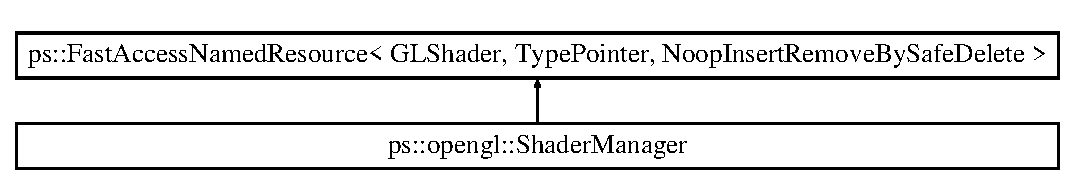
\includegraphics[height=2.000000cm]{classps_1_1opengl_1_1ShaderManager}
\end{center}
\end{figure}
\subsection*{Public Member Functions}
\begin{DoxyCompactItemize}
\item 
\hypertarget{classps_1_1opengl_1_1ShaderManager_a5a8abca6e977d92f965fd8e3c221be0b}{}bool {\bfseries add} (const char $\ast$name, const char $\ast$v\+Shader\+Code, const char $\ast$f\+Shader\+Code, const char $\ast$g\+Shader\+Code=N\+U\+L\+L)\label{classps_1_1opengl_1_1ShaderManager_a5a8abca6e977d92f965fd8e3c221be0b}

\item 
\hypertarget{classps_1_1opengl_1_1ShaderManager_a94645c29abc9d73b2ca3d859076cca78}{}bool {\bfseries add\+From\+File} (const char $\ast$name, const \hyperlink{classps_1_1base_1_1CAString}{Ansi\+Str} \&str\+V\+Shader\+F\+P, const \hyperlink{classps_1_1base_1_1CAString}{Ansi\+Str} \&str\+F\+Shader\+F\+P)\label{classps_1_1opengl_1_1ShaderManager_a94645c29abc9d73b2ca3d859076cca78}

\item 
\hypertarget{classps_1_1opengl_1_1ShaderManager_a2132b94083c5865219aafc1dac3b7e9c}{}bool {\bfseries add\+From\+File} (const char $\ast$name, const \hyperlink{classps_1_1base_1_1CAString}{Ansi\+Str} \&str\+V\+Shader\+F\+P, const \hyperlink{classps_1_1base_1_1CAString}{Ansi\+Str} \&str\+F\+Shader\+F\+P, const \hyperlink{classps_1_1base_1_1CAString}{Ansi\+Str} \&str\+G\+Shader\+F\+P)\label{classps_1_1opengl_1_1ShaderManager_a2132b94083c5865219aafc1dac3b7e9c}

\item 
\hypertarget{classps_1_1opengl_1_1ShaderManager_a1541525affb88e834f39d0130c2a6cee}{}int {\bfseries add\+From\+Folder} (const char $\ast$chr\+Shaders\+Path)\label{classps_1_1opengl_1_1ShaderManager_a1541525affb88e834f39d0130c2a6cee}

\end{DoxyCompactItemize}
\subsection*{Additional Inherited Members}


The documentation for this class was generated from the following files\+:\begin{DoxyCompactItemize}
\item 
/\+Users/pourya/\+Desktop/platform/repos/tetcutter/src/glbackend/glshadermanager.\+h\item 
/\+Users/pourya/\+Desktop/platform/repos/tetcutter/src/glbackend/glshadermanager.\+cpp\end{DoxyCompactItemize}

\hypertarget{structps_1_1opengl_1_1ShaderNoopInsertGLRemove}{}\section{ps\+:\+:opengl\+:\+:Shader\+Noop\+Insert\+G\+L\+Remove$<$ T $>$ Struct Template Reference}
\label{structps_1_1opengl_1_1ShaderNoopInsertGLRemove}\index{ps\+::opengl\+::\+Shader\+Noop\+Insert\+G\+L\+Remove$<$ T $>$@{ps\+::opengl\+::\+Shader\+Noop\+Insert\+G\+L\+Remove$<$ T $>$}}
\subsection*{Static Public Member Functions}
\begin{DoxyCompactItemize}
\item 
\hypertarget{structps_1_1opengl_1_1ShaderNoopInsertGLRemove_a5817e67ba205a26ab8c331f22840a4b0}{}static void {\bfseries Insert} (T element)\label{structps_1_1opengl_1_1ShaderNoopInsertGLRemove_a5817e67ba205a26ab8c331f22840a4b0}

\item 
\hypertarget{structps_1_1opengl_1_1ShaderNoopInsertGLRemove_a3e9c3dbcddc6170f6fd204336c07201b}{}static void {\bfseries Remove} (T element)\label{structps_1_1opengl_1_1ShaderNoopInsertGLRemove_a3e9c3dbcddc6170f6fd204336c07201b}

\end{DoxyCompactItemize}


The documentation for this struct was generated from the following file\+:\begin{DoxyCompactItemize}
\item 
/\+Users/pourya/\+Desktop/platform/repos/tetcutter/src/glbackend/glshadermanager.\+h\end{DoxyCompactItemize}

\hypertarget{classps_1_1elastic_1_1TestVolMesh}{}\section{ps\+:\+:elastic\+:\+:Test\+Vol\+Mesh Class Reference}
\label{classps_1_1elastic_1_1TestVolMesh}\index{ps\+::elastic\+::\+Test\+Vol\+Mesh@{ps\+::elastic\+::\+Test\+Vol\+Mesh}}


{\ttfamily \#include $<$test\+\_\+volmesh.\+h$>$}

\subsection*{Static Public Member Functions}
\begin{DoxyCompactItemize}
\item 
\hypertarget{classps_1_1elastic_1_1TestVolMesh_ac4aca05e1e19b77a262b7b9d90224481}{}static bool {\bfseries tst\+\_\+report\+\_\+mesh\+\_\+info} (\hyperlink{classps_1_1elastic_1_1VolMesh}{Vol\+Mesh} $\ast$pmesh)\label{classps_1_1elastic_1_1TestVolMesh_ac4aca05e1e19b77a262b7b9d90224481}

\item 
\hypertarget{classps_1_1elastic_1_1TestVolMesh_a25899cb9d6ae6dec5d5dd3290f638436}{}static bool {\bfseries tst\+\_\+correct\+\_\+elements} (\hyperlink{classps_1_1elastic_1_1VolMesh}{Vol\+Mesh} $\ast$pmesh)\label{classps_1_1elastic_1_1TestVolMesh_a25899cb9d6ae6dec5d5dd3290f638436}

\item 
\hypertarget{classps_1_1elastic_1_1TestVolMesh_a4833d63cfdff1b6c5bcd93f415e2074c}{}static bool {\bfseries tst\+\_\+unused\+\_\+mesh\+\_\+fields} (\hyperlink{classps_1_1elastic_1_1VolMesh}{Vol\+Mesh} $\ast$pmesh)\label{classps_1_1elastic_1_1TestVolMesh_a4833d63cfdff1b6c5bcd93f415e2074c}

\item 
\hypertarget{classps_1_1elastic_1_1TestVolMesh_a6f7436bd71970bac4572c10958dbff61}{}static bool {\bfseries tst\+\_\+connectivity} (\hyperlink{classps_1_1elastic_1_1VolMesh}{Vol\+Mesh} $\ast$pmesh)\label{classps_1_1elastic_1_1TestVolMesh_a6f7436bd71970bac4572c10958dbff61}

\item 
\hypertarget{classps_1_1elastic_1_1TestVolMesh_ae780054129c87ad1c9f36ece6729887d}{}static bool {\bfseries tst\+\_\+all} (\hyperlink{classps_1_1elastic_1_1VolMesh}{Vol\+Mesh} $\ast$pmesh)\label{classps_1_1elastic_1_1TestVolMesh_ae780054129c87ad1c9f36ece6729887d}

\end{DoxyCompactItemize}


\subsection{Detailed Description}
east test returns true if successful and false otherwise 

The documentation for this class was generated from the following files\+:\begin{DoxyCompactItemize}
\item 
/\+Users/pourya/\+Desktop/platform/repos/tetcutter/src/elastic/test\+\_\+volmesh.\+h\item 
/\+Users/pourya/\+Desktop/platform/repos/tetcutter/src/elastic/test\+\_\+volmesh.\+cpp\end{DoxyCompactItemize}

\hypertarget{classps_1_1elastic_1_1TetSubdivider}{}\section{ps\+:\+:elastic\+:\+:Tet\+Subdivider Class Reference}
\label{classps_1_1elastic_1_1TetSubdivider}\index{ps\+::elastic\+::\+Tet\+Subdivider@{ps\+::elastic\+::\+Tet\+Subdivider}}
Inheritance diagram for ps\+:\+:elastic\+:\+:Tet\+Subdivider\+:\begin{figure}[H]
\begin{center}
\leavevmode
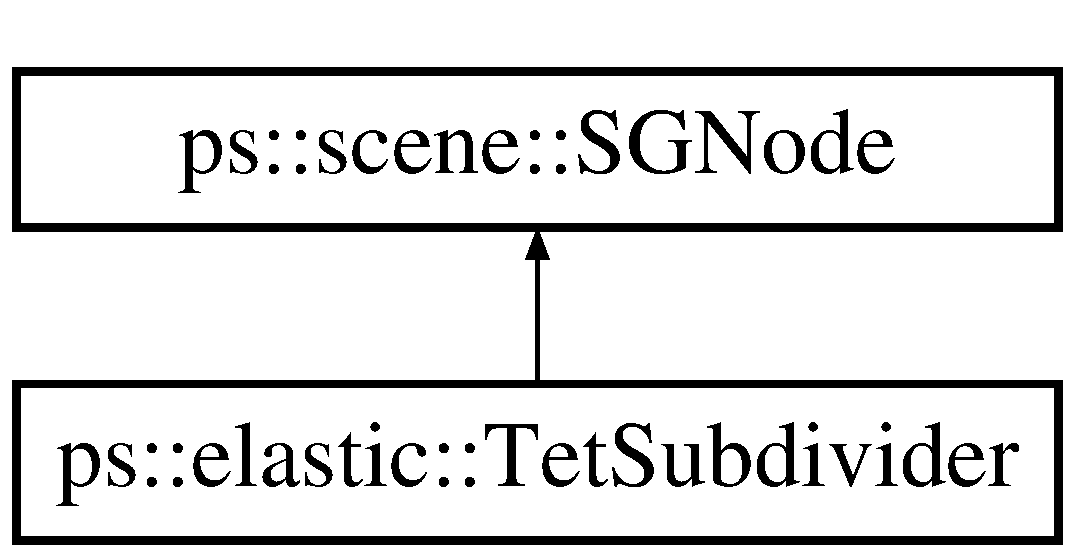
\includegraphics[height=2.000000cm]{classps_1_1elastic_1_1TetSubdivider}
\end{center}
\end{figure}
\subsection*{Public Types}
\begin{DoxyCompactItemize}
\item 
\hypertarget{classps_1_1elastic_1_1TetSubdivider_a237979de41e5e60582f653399d1cb477}{}enum {\bfseries C\+U\+T\+C\+A\+S\+E} \{ \\*
{\bfseries cut\+A}, 
{\bfseries cut\+B}, 
{\bfseries cut\+C}, 
{\bfseries cut\+D}, 
\\*
{\bfseries cut\+E}, 
{\bfseries cut\+X}, 
{\bfseries cut\+Y}, 
{\bfseries cut\+Z}, 
\\*
{\bfseries cut\+Unknown}
 \}\label{classps_1_1elastic_1_1TetSubdivider_a237979de41e5e60582f653399d1cb477}

\end{DoxyCompactItemize}
\subsection*{Public Member Functions}
\begin{DoxyCompactItemize}
\item 
\hypertarget{classps_1_1elastic_1_1TetSubdivider_ab498e762dd8a4789ace462a881a7ae7b}{}void {\bfseries draw} ()\label{classps_1_1elastic_1_1TetSubdivider_ab498e762dd8a4789ace462a881a7ae7b}

\item 
\hypertarget{classps_1_1elastic_1_1TetSubdivider_affebbf7aa37abee39f105b2d80f71173}{}char {\bfseries to\+Alpha} (C\+U\+T\+C\+A\+S\+E c)\label{classps_1_1elastic_1_1TetSubdivider_affebbf7aa37abee39f105b2d80f71173}

\item 
\hypertarget{classps_1_1elastic_1_1TetSubdivider_a5814ddced3c53946587b7226fdd45d99}{}int {\bfseries subdivide} (\hyperlink{classps_1_1elastic_1_1VolMesh}{Vol\+Mesh} $\ast$pmesh, U32 idx\+Cell, U8 cut\+Edge\+Code, U8 cut\+Node\+Code, U32 mid\+Nodes\mbox{[}12\mbox{]})\label{classps_1_1elastic_1_1TetSubdivider_a5814ddced3c53946587b7226fdd45d99}

\item 
\hypertarget{classps_1_1elastic_1_1TetSubdivider_a195dbc4807e828bee0609d9fc54cacad}{}int \hyperlink{classps_1_1elastic_1_1TetSubdivider_a195dbc4807e828bee0609d9fc54cacad}{generate\+Case\+A} (\hyperlink{classps_1_1elastic_1_1VolMesh}{Vol\+Mesh} $\ast$pmesh, U32 idx\+Cell, U8 node, double target\+Dist\+Percentage, U8 \&cut\+Edge\+Code, U8 \&cut\+Node\+Code)\label{classps_1_1elastic_1_1TetSubdivider_a195dbc4807e828bee0609d9fc54cacad}

\begin{DoxyCompactList}\small\item\em generates case A where a node in separated from the rest of the element. 3 edges are cut. \+: element to be considered \+: the node to be separated \+: distance to the node \mbox{[}0-\/1\mbox{]} \+: output cutedge code \end{DoxyCompactList}\item 
\hypertarget{classps_1_1elastic_1_1TetSubdivider_abd5e58f8e350350189dac343d27d4793}{}int \hyperlink{classps_1_1elastic_1_1TetSubdivider_abd5e58f8e350350189dac343d27d4793}{generate\+Case\+B} (\hyperlink{classps_1_1elastic_1_1VolMesh}{Vol\+Mesh} $\ast$pmesh, U32 idx\+Cell, U8 enteringface, U8 \&cut\+Edge\+Code, U8 \&cut\+Node\+Code)\label{classps_1_1elastic_1_1TetSubdivider_abd5e58f8e350350189dac343d27d4793}

\begin{DoxyCompactList}\small\item\em generates case B where an element is sliced into two sections by cutting its 4 edges. There 3 different case that can produce this state \+: tetrahedral element to be considered \+: start face which can be 0, 1 or 2 (end face is 3) \+: output cutedge code \+: output cutnode code \+: the distance over the edges where the cuts are happening \end{DoxyCompactList}\item 
\hypertarget{classps_1_1elastic_1_1TetSubdivider_ae2278f898eb67a69857523183ab70765}{}bool {\bfseries write\+Look\+Up\+Table} ()\label{classps_1_1elastic_1_1TetSubdivider_ae2278f898eb67a69857523183ab70765}

\end{DoxyCompactItemize}
\subsection*{Static Public Member Functions}
\begin{DoxyCompactItemize}
\item 
\hypertarget{classps_1_1elastic_1_1TetSubdivider_a0102d85c9bfa1194fe5172b067e354df}{}static C\+U\+T\+C\+A\+S\+E {\bfseries Identify\+Cut\+Case} (bool is\+Cut\+Complete, U8 cut\+Edge\+Code, U8 cut\+Node\+Code)\label{classps_1_1elastic_1_1TetSubdivider_a0102d85c9bfa1194fe5172b067e354df}

\item 
\hypertarget{classps_1_1elastic_1_1TetSubdivider_a62c3596bb90ef76362552c62c92c290c}{}static C\+U\+T\+C\+A\+S\+E {\bfseries Identify\+Cut\+Case} (bool is\+Cut\+Complete, U8 cut\+Edge\+Code, U8 cut\+Node\+Code, U8 \&count\+Cut\+Edges, U8 \&count\+Cut\+Nodes)\label{classps_1_1elastic_1_1TetSubdivider_a62c3596bb90ef76362552c62c92c290c}

\end{DoxyCompactItemize}
\subsection*{Protected Attributes}
\begin{DoxyCompactItemize}
\item 
\hypertarget{classps_1_1elastic_1_1TetSubdivider_a293adbce753900f3d2d1197b2e3ded54}{}std\+::map$<$ U8, int $>$ {\bfseries m\+\_\+map\+Cut\+Edge\+Code\+To\+Table\+Entry}\label{classps_1_1elastic_1_1TetSubdivider_a293adbce753900f3d2d1197b2e3ded54}

\item 
\hypertarget{classps_1_1elastic_1_1TetSubdivider_af03c8a2d7564db4769a28528105c6935}{}std\+::map$<$ Tet\+Subdivider\+::\+C\+U\+T\+C\+A\+S\+E, char $>$ {\bfseries m\+\_\+map\+Cut\+Case\+To\+Alpha}\label{classps_1_1elastic_1_1TetSubdivider_af03c8a2d7564db4769a28528105c6935}

\end{DoxyCompactItemize}


The documentation for this class was generated from the following files\+:\begin{DoxyCompactItemize}
\item 
/\+Users/pourya/\+Desktop/platform/repos/tetcutter/src/elastic/tetsubdivider.\+h\item 
/\+Users/pourya/\+Desktop/platform/repos/tetcutter/src/elastic/tetsubdivider.\+cpp\end{DoxyCompactItemize}

\hypertarget{classps_1_1opengl_1_1TexManager}{}\section{ps\+:\+:opengl\+:\+:Tex\+Manager Class Reference}
\label{classps_1_1opengl_1_1TexManager}\index{ps\+::opengl\+::\+Tex\+Manager@{ps\+::opengl\+::\+Tex\+Manager}}
Inheritance diagram for ps\+:\+:opengl\+:\+:Tex\+Manager\+:\begin{figure}[H]
\begin{center}
\leavevmode
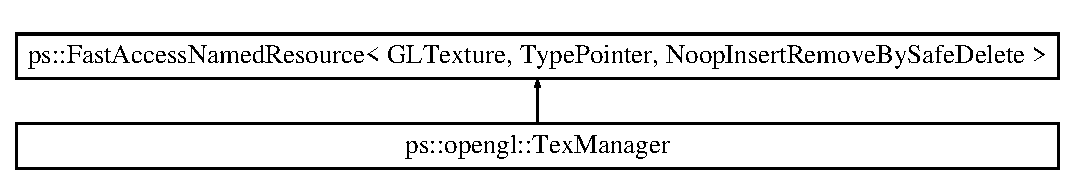
\includegraphics[height=2.000000cm]{classps_1_1opengl_1_1TexManager}
\end{center}
\end{figure}
\subsection*{Public Member Functions}
\begin{DoxyCompactItemize}
\item 
\hypertarget{classps_1_1opengl_1_1TexManager_aadd48e37b3a865c93cf91a8add45aa35}{}bool {\bfseries add} (const \hyperlink{classps_1_1base_1_1CAString}{Ansi\+Str} \&str\+F\+P)\label{classps_1_1opengl_1_1TexManager_aadd48e37b3a865c93cf91a8add45aa35}

\end{DoxyCompactItemize}
\subsection*{Additional Inherited Members}


The documentation for this class was generated from the following files\+:\begin{DoxyCompactItemize}
\item 
/\+Users/pourya/\+Desktop/platform/repos/tetcutter/src/glbackend/gltexturemanager.\+h\item 
/\+Users/pourya/\+Desktop/platform/repos/tetcutter/src/glbackend/gltexturemanager.\+cpp\end{DoxyCompactItemize}

\hypertarget{classps_1_1elastic_1_1TexturedEffect}{}\section{ps\+:\+:elastic\+:\+:Textured\+Effect Class Reference}
\label{classps_1_1elastic_1_1TexturedEffect}\index{ps\+::elastic\+::\+Textured\+Effect@{ps\+::elastic\+::\+Textured\+Effect}}
Inheritance diagram for ps\+:\+:elastic\+:\+:Textured\+Effect\+:\begin{figure}[H]
\begin{center}
\leavevmode
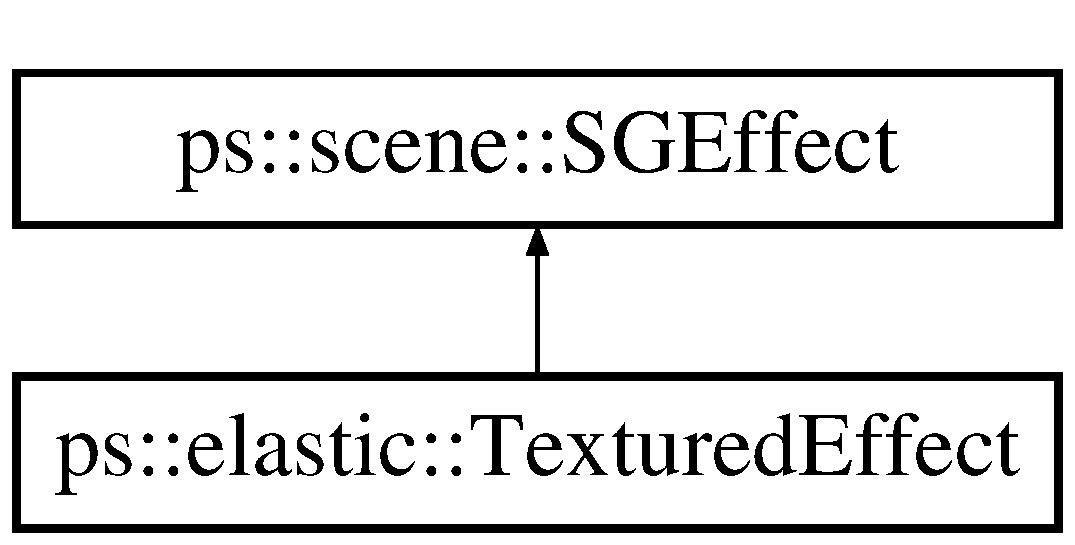
\includegraphics[height=2.000000cm]{classps_1_1elastic_1_1TexturedEffect}
\end{center}
\end{figure}
\subsection*{Public Member Functions}
\begin{DoxyCompactItemize}
\item 
\hypertarget{classps_1_1elastic_1_1TexturedEffect_a1f702b5416e161ea73964c155eed6ca3}{}{\bfseries Textured\+Effect} (\hyperlink{classps_1_1opengl_1_1GLShader}{G\+L\+Shader} $\ast$s)\label{classps_1_1elastic_1_1TexturedEffect_a1f702b5416e161ea73964c155eed6ca3}

\item 
\hypertarget{classps_1_1elastic_1_1TexturedEffect_a127d4d9b456d658706985bc794a9c943}{}void {\bfseries bind} ()\label{classps_1_1elastic_1_1TexturedEffect_a127d4d9b456d658706985bc794a9c943}

\end{DoxyCompactItemize}
\subsection*{Additional Inherited Members}


The documentation for this class was generated from the following file\+:\begin{DoxyCompactItemize}
\item 
/\+Users/pourya/\+Desktop/platform/repos/tetcutter/src/elastic/avatarring.\+cpp\end{DoxyCompactItemize}

\hypertarget{classps_1_1scene_1_1TexturedEffect}{}\section{ps\+:\+:scene\+:\+:Textured\+Effect Class Reference}
\label{classps_1_1scene_1_1TexturedEffect}\index{ps\+::scene\+::\+Textured\+Effect@{ps\+::scene\+::\+Textured\+Effect}}
Inheritance diagram for ps\+:\+:scene\+:\+:Textured\+Effect\+:\begin{figure}[H]
\begin{center}
\leavevmode
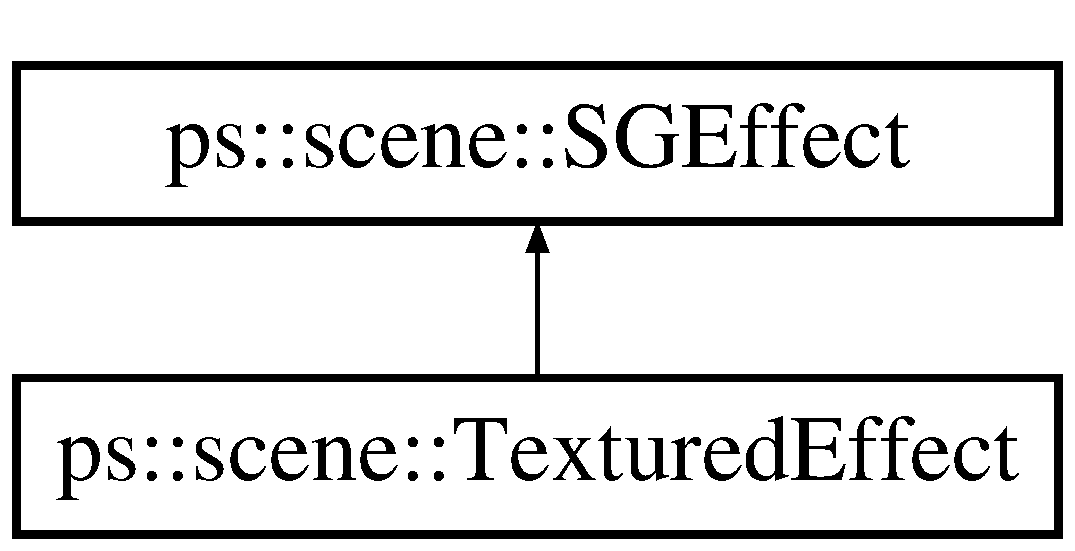
\includegraphics[height=2.000000cm]{classps_1_1scene_1_1TexturedEffect}
\end{center}
\end{figure}
\subsection*{Public Member Functions}
\begin{DoxyCompactItemize}
\item 
\hypertarget{classps_1_1scene_1_1TexturedEffect_af378b17f296976df86c5e42d5d34ab8b}{}{\bfseries Textured\+Effect} (\hyperlink{classps_1_1opengl_1_1GLShader}{G\+L\+Shader} $\ast$s)\label{classps_1_1scene_1_1TexturedEffect_af378b17f296976df86c5e42d5d34ab8b}

\item 
\hypertarget{classps_1_1scene_1_1TexturedEffect_a97a35e1448b34688a3c1bccb3709b117}{}void {\bfseries bind} ()\label{classps_1_1scene_1_1TexturedEffect_a97a35e1448b34688a3c1bccb3709b117}

\end{DoxyCompactItemize}
\subsection*{Additional Inherited Members}


The documentation for this class was generated from the following file\+:\begin{DoxyCompactItemize}
\item 
/\+Users/pourya/\+Desktop/platform/repos/tetcutter/src/scene/sgquad.\+cpp\end{DoxyCompactItemize}

\hypertarget{structps_1_1TypePointer}{}\section{ps\+:\+:Type\+Pointer$<$ T $>$ Struct Template Reference}
\label{structps_1_1TypePointer}\index{ps\+::\+Type\+Pointer$<$ T $>$@{ps\+::\+Type\+Pointer$<$ T $>$}}
\subsection*{Public Types}
\begin{DoxyCompactItemize}
\item 
\hypertarget{structps_1_1TypePointer_aa119db5b38f5c3da204800b750857876}{}typedef T $\ast$ {\bfseries Resource}\label{structps_1_1TypePointer_aa119db5b38f5c3da204800b750857876}

\end{DoxyCompactItemize}


The documentation for this struct was generated from the following file\+:\begin{DoxyCompactItemize}
\item 
/\+Users/pourya/\+Desktop/platform/repos/tetcutter/src/base/resourcemanager.\+h\end{DoxyCompactItemize}

\hypertarget{structps_1_1TypeValue}{}\section{ps\+:\+:Type\+Value$<$ T $>$ Struct Template Reference}
\label{structps_1_1TypeValue}\index{ps\+::\+Type\+Value$<$ T $>$@{ps\+::\+Type\+Value$<$ T $>$}}
\subsection*{Public Types}
\begin{DoxyCompactItemize}
\item 
\hypertarget{structps_1_1TypeValue_a5584d02559097a9c20ba0f9a160b6df2}{}typedef T {\bfseries Resource}\label{structps_1_1TypeValue_a5584d02559097a9c20ba0f9a160b6df2}

\end{DoxyCompactItemize}


The documentation for this struct was generated from the following file\+:\begin{DoxyCompactItemize}
\item 
/\+Users/pourya/\+Desktop/platform/repos/tetcutter/src/base/resourcemanager.\+h\end{DoxyCompactItemize}

\hypertarget{classps_1_1Value}{}\section{ps\+:\+:Value Class Reference}
\label{classps_1_1Value}\index{ps\+::\+Value@{ps\+::\+Value}}
\subsection*{Public Member Functions}
\begin{DoxyCompactItemize}
\item 
\hypertarget{classps_1_1Value_a7a5a409ab6504185ead8845776099089}{}{\footnotesize template$<$typename value\+\_\+type $>$ }\\{\bfseries Value} (const value\+\_\+type \&v)\label{classps_1_1Value_a7a5a409ab6504185ead8845776099089}

\item 
\hypertarget{classps_1_1Value_a4583b0d7308114e9605fe1376058aa37}{}{\bfseries Value} (const \hyperlink{classps_1_1Value}{Value} \&other)\label{classps_1_1Value_a4583b0d7308114e9605fe1376058aa37}

\item 
\hypertarget{classps_1_1Value_a6e60171a80e82933e20dc0bdc0b62c8b}{}const std\+::type\+\_\+info \& {\bfseries type\+\_\+info} () const \label{classps_1_1Value_a6e60171a80e82933e20dc0bdc0b62c8b}

\item 
\hypertarget{classps_1_1Value_a9ecf352c01a0d066fc44082bb73ecd85}{}const std\+::string {\bfseries to\+String} () const \label{classps_1_1Value_a9ecf352c01a0d066fc44082bb73ecd85}

\item 
\hypertarget{classps_1_1Value_ad0aa50b9966f7a54735815d85f4555c9}{}void {\bfseries from\+String} (const string \&s)\label{classps_1_1Value_ad0aa50b9966f7a54735815d85f4555c9}

\item 
\hypertarget{classps_1_1Value_a8c51ad5966394e8eca48e32866d79a47}{}{\footnotesize template$<$typename value\+\_\+type $>$ }\\value\+\_\+type {\bfseries get} () const \label{classps_1_1Value_a8c51ad5966394e8eca48e32866d79a47}

\item 
\hypertarget{classps_1_1Value_ada466d6d562f9c44cb46fe5377ef4eb6}{}{\footnotesize template$<$typename value\+\_\+type $>$ }\\const value\+\_\+type $\ast$ {\bfseries cptr} () const \label{classps_1_1Value_ada466d6d562f9c44cb46fe5377ef4eb6}

\item 
\hypertarget{classps_1_1Value_a4fc174cf24bc7872eb2692652bc90e48}{}\hyperlink{classps_1_1Value}{Value} \& {\bfseries swap} (\hyperlink{classps_1_1Value}{Value} \&rhs)\label{classps_1_1Value_a4fc174cf24bc7872eb2692652bc90e48}

\item 
\hypertarget{classps_1_1Value_a4d97c97b44a48644cc9e6de01b033b0d}{}\hyperlink{classps_1_1Value}{Value} \& {\bfseries operator=} (const \hyperlink{classps_1_1Value}{Value} \&rhs)\label{classps_1_1Value_a4d97c97b44a48644cc9e6de01b033b0d}

\item 
\hypertarget{classps_1_1Value_a3acf820a982de257bd77cb6f75f9f030}{}{\footnotesize template$<$typename value\+\_\+type $>$ }\\\hyperlink{classps_1_1Value}{Value} \& {\bfseries operator=} (const value\+\_\+type \&rhs)\label{classps_1_1Value_a3acf820a982de257bd77cb6f75f9f030}

\item 
\hypertarget{classps_1_1Value_a5211288c17607a29258ca905a3769539}{}{\bfseries operator const void $\ast$} () const \label{classps_1_1Value_a5211288c17607a29258ca905a3769539}

\end{DoxyCompactItemize}


The documentation for this class was generated from the following file\+:\begin{DoxyCompactItemize}
\item 
/\+Users/pourya/\+Desktop/platform/repos/tetcutter/src/base/value.\+h\end{DoxyCompactItemize}

\hypertarget{classps_1_1ValueStorage}{}\section{ps\+:\+:Value\+Storage Class Reference}
\label{classps_1_1ValueStorage}\index{ps\+::\+Value\+Storage@{ps\+::\+Value\+Storage}}
Inheritance diagram for ps\+:\+:Value\+Storage\+:\begin{figure}[H]
\begin{center}
\leavevmode
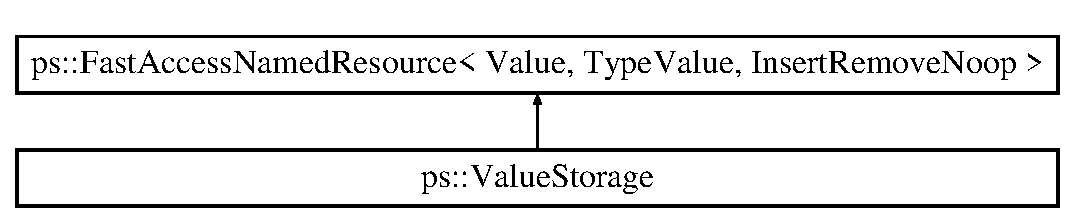
\includegraphics[height=2.000000cm]{classps_1_1ValueStorage}
\end{center}
\end{figure}
\subsection*{Public Member Functions}
\begin{DoxyCompactItemize}
\item 
\hypertarget{classps_1_1ValueStorage_a683e7c7eaf6eb51811ba3b6dcbfeaad8}{}void {\bfseries print\+All} ()\label{classps_1_1ValueStorage_a683e7c7eaf6eb51811ba3b6dcbfeaad8}

\item 
\hypertarget{classps_1_1ValueStorage_ae1dc01f5d76d1d1f037e1ca330f3b8d8}{}virtual bool {\bfseries read} (const \hyperlink{classps_1_1base_1_1CAString}{Ansi\+Str} \&str\+F\+P)\label{classps_1_1ValueStorage_ae1dc01f5d76d1d1f037e1ca330f3b8d8}

\item 
\hypertarget{classps_1_1ValueStorage_a95a94b2b4bbed02ab26185ae1ba8f926}{}virtual bool {\bfseries write} (const \hyperlink{classps_1_1base_1_1CAString}{Ansi\+Str} \&str\+F\+P)\label{classps_1_1ValueStorage_a95a94b2b4bbed02ab26185ae1ba8f926}

\item 
\hypertarget{classps_1_1ValueStorage_a43014a4a189cda8ef9498edfe19993a8}{}virtual bool {\bfseries read\+Script} (const \hyperlink{classps_1_1base_1_1CAString}{Ansi\+Str} \&str\+F\+P, const \hyperlink{classps_1_1base_1_1CAString}{Ansi\+Str} \&section=\char`\"{}G\+E\+N\+E\+R\+A\+L\char`\"{})\label{classps_1_1ValueStorage_a43014a4a189cda8ef9498edfe19993a8}

\item 
\hypertarget{classps_1_1ValueStorage_a0d002ab47d51649919643afcc16b7f61}{}virtual bool {\bfseries write\+Script} (const \hyperlink{classps_1_1base_1_1CAString}{Ansi\+Str} \&str\+F\+P, const \hyperlink{classps_1_1base_1_1CAString}{Ansi\+Str} \&section=\char`\"{}G\+E\+N\+E\+R\+A\+L\char`\"{})\label{classps_1_1ValueStorage_a0d002ab47d51649919643afcc16b7f61}

\end{DoxyCompactItemize}
\subsection*{Additional Inherited Members}


The documentation for this class was generated from the following files\+:\begin{DoxyCompactItemize}
\item 
/\+Users/pourya/\+Desktop/platform/repos/tetcutter/src/base/valuestorage.\+h\item 
/\+Users/pourya/\+Desktop/platform/repos/tetcutter/src/base/valuestorage.\+cpp\end{DoxyCompactItemize}

\hypertarget{structps_1_1opengl_1_1GLShader_1_1VARPROP}{}\section{ps\+:\+:opengl\+:\+:G\+L\+Shader\+:\+:V\+A\+R\+P\+R\+O\+P Struct Reference}
\label{structps_1_1opengl_1_1GLShader_1_1VARPROP}\index{ps\+::opengl\+::\+G\+L\+Shader\+::\+V\+A\+R\+P\+R\+O\+P@{ps\+::opengl\+::\+G\+L\+Shader\+::\+V\+A\+R\+P\+R\+O\+P}}
\subsection*{Public Attributes}
\begin{DoxyCompactItemize}
\item 
\hypertarget{structps_1_1opengl_1_1GLShader_1_1VARPROP_aaae917d30bc1da64325ab09c55dedc74}{}\hyperlink{classps_1_1base_1_1CAString}{Ansi\+Str} {\bfseries str\+Name}\label{structps_1_1opengl_1_1GLShader_1_1VARPROP_aaae917d30bc1da64325ab09c55dedc74}

\item 
\hypertarget{structps_1_1opengl_1_1GLShader_1_1VARPROP_a4f9919cb26bf4b102aac16349bd54bdf}{}\hyperlink{classps_1_1base_1_1CAString}{Ansi\+Str} {\bfseries str\+Type}\label{structps_1_1opengl_1_1GLShader_1_1VARPROP_a4f9919cb26bf4b102aac16349bd54bdf}

\item 
\hypertarget{structps_1_1opengl_1_1GLShader_1_1VARPROP_ae26a88b405fc5ddd66eb1324b5b75aa5}{}V\+A\+R\+U\+S\+A\+G\+E {\bfseries usage}\label{structps_1_1opengl_1_1GLShader_1_1VARPROP_ae26a88b405fc5ddd66eb1324b5b75aa5}

\item 
\hypertarget{structps_1_1opengl_1_1GLShader_1_1VARPROP_a5c1e1e1689b3db0c57c766beaab05c4a}{}V\+A\+R\+P\+R\+E\+C\+I\+S\+I\+O\+N {\bfseries precision}\label{structps_1_1opengl_1_1GLShader_1_1VARPROP_a5c1e1e1689b3db0c57c766beaab05c4a}

\item 
\hypertarget{structps_1_1opengl_1_1GLShader_1_1VARPROP_a418991e949e8c8076723a496c0c19ace}{}int {\bfseries idx\+Location}\label{structps_1_1opengl_1_1GLShader_1_1VARPROP_a418991e949e8c8076723a496c0c19ace}

\end{DoxyCompactItemize}


The documentation for this struct was generated from the following file\+:\begin{DoxyCompactItemize}
\item 
/\+Users/pourya/\+Desktop/platform/repos/tetcutter/src/glbackend/glshader.\+h\end{DoxyCompactItemize}

\hypertarget{classps_1_1base_1_1Vec2}{}\section{ps\+:\+:base\+:\+:Vec2$<$ T $>$ Class Template Reference}
\label{classps_1_1base_1_1Vec2}\index{ps\+::base\+::\+Vec2$<$ T $>$@{ps\+::base\+::\+Vec2$<$ T $>$}}


{\ttfamily \#include $<$vec.\+h$>$}

\subsection*{Public Member Functions}
\begin{DoxyCompactItemize}
\item 
\hypertarget{classps_1_1base_1_1Vec2_a46d716c24263488aa1df44335374c7dd}{}{\bfseries Vec2} (T x\+\_\+, T y\+\_\+)\label{classps_1_1base_1_1Vec2_a46d716c24263488aa1df44335374c7dd}

\item 
\hypertarget{classps_1_1base_1_1Vec2_a1fe26daa86abde821027bb5b17a25d1a}{}{\bfseries Vec2} (const \hyperlink{classps_1_1base_1_1Vec2}{Vec2} \&rhs)\label{classps_1_1base_1_1Vec2_a1fe26daa86abde821027bb5b17a25d1a}

\item 
\hypertarget{classps_1_1base_1_1Vec2_adb4da2eae9f689778f1fee47925a4028}{}{\bfseries Vec2} (const T $\ast$p\+Values)\label{classps_1_1base_1_1Vec2_adb4da2eae9f689778f1fee47925a4028}

\item 
\hypertarget{classps_1_1base_1_1Vec2_a3422a88f805299ac944d6774c9240ec0}{}void {\bfseries load} (const T $\ast$p\+Values)\label{classps_1_1base_1_1Vec2_a3422a88f805299ac944d6774c9240ec0}

\item 
\hypertarget{classps_1_1base_1_1Vec2_a1a462bdb77e1004901e30c9c5e7c45dc}{}void {\bfseries store} (const T $\ast$p\+Values) const \label{classps_1_1base_1_1Vec2_a1a462bdb77e1004901e30c9c5e7c45dc}

\item 
\hypertarget{classps_1_1base_1_1Vec2_a5efe8321c15342528c57570bca1f48e3}{}void {\bfseries normalize} ()\label{classps_1_1base_1_1Vec2_a5efe8321c15342528c57570bca1f48e3}

\item 
\hypertarget{classps_1_1base_1_1Vec2_ab626f986b91fb3b942d4ca1662216fe9}{}\hyperlink{classps_1_1base_1_1Vec2}{Vec2} {\bfseries normalized} () const \label{classps_1_1base_1_1Vec2_ab626f986b91fb3b942d4ca1662216fe9}

\item 
\hypertarget{classps_1_1base_1_1Vec2_ae494ef913dcacb7b41859eaafbe8f283}{}T {\bfseries length} () const \label{classps_1_1base_1_1Vec2_ae494ef913dcacb7b41859eaafbe8f283}

\item 
\hypertarget{classps_1_1base_1_1Vec2_a4d5a821cd0b792666912f0e28a4d5960}{}T {\bfseries length2} () const \label{classps_1_1base_1_1Vec2_a4d5a821cd0b792666912f0e28a4d5960}

\item 
\hypertarget{classps_1_1base_1_1Vec2_aaa003d7243c2d28de85994b303d9a54b}{}T {\bfseries element} (int i) const \label{classps_1_1base_1_1Vec2_aaa003d7243c2d28de85994b303d9a54b}

\item 
\hypertarget{classps_1_1base_1_1Vec2_a0fefdecc9dbe852999b31557df60d135}{}void {\bfseries set\+Element} (int i, T v)\label{classps_1_1base_1_1Vec2_a0fefdecc9dbe852999b31557df60d135}

\item 
\hypertarget{classps_1_1base_1_1Vec2_a98bd696ec9034ec793054cbf67a433b9}{}int {\bfseries longest\+Axis} () const \label{classps_1_1base_1_1Vec2_a98bd696ec9034ec793054cbf67a433b9}

\item 
\hypertarget{classps_1_1base_1_1Vec2_a0a49df938758f32883bc17c0ad9b5ae8}{}T $\ast$ {\bfseries ptr} ()\label{classps_1_1base_1_1Vec2_a0a49df938758f32883bc17c0ad9b5ae8}

\item 
\hypertarget{classps_1_1base_1_1Vec2_a006f8d8b0eff11db3d3c00a364c07498}{}const T $\ast$ {\bfseries cptr} () const \label{classps_1_1base_1_1Vec2_a006f8d8b0eff11db3d3c00a364c07498}

\item 
\hypertarget{classps_1_1base_1_1Vec2_a258789dee8928eb61f79893022b7b2d6}{}\hyperlink{classps_1_1base_1_1Vec2}{Vec2} \& {\bfseries operator=} (const \hyperlink{classps_1_1base_1_1Vec2}{Vec2} \&rhs)\label{classps_1_1base_1_1Vec2_a258789dee8928eb61f79893022b7b2d6}

\item 
\hypertarget{classps_1_1base_1_1Vec2_a8e7a77b279c4152acdcbb912ac547c26}{}\hyperlink{classps_1_1base_1_1Vec2}{Vec2} {\bfseries operator$\ast$} (T s) const \label{classps_1_1base_1_1Vec2_a8e7a77b279c4152acdcbb912ac547c26}

\item 
\hypertarget{classps_1_1base_1_1Vec2_a886d97601702afef58146775aa721291}{}\hyperlink{classps_1_1base_1_1Vec2}{Vec2} {\bfseries operator+} (const \hyperlink{classps_1_1base_1_1Vec2}{Vec2} \&rhs) const \label{classps_1_1base_1_1Vec2_a886d97601702afef58146775aa721291}

\item 
\hypertarget{classps_1_1base_1_1Vec2_ac11a6c1d8b6d804ac40d606e5c67d84c}{}\hyperlink{classps_1_1base_1_1Vec2}{Vec2} {\bfseries operator-\/} (const \hyperlink{classps_1_1base_1_1Vec2}{Vec2} \&rhs) const \label{classps_1_1base_1_1Vec2_ac11a6c1d8b6d804ac40d606e5c67d84c}

\item 
\hypertarget{classps_1_1base_1_1Vec2_a8cf67f172b65100e77ee06f0611a1bc6}{}bool {\bfseries operator==} (const \hyperlink{classps_1_1base_1_1Vec2}{Vec2} \&rhs) const \label{classps_1_1base_1_1Vec2_a8cf67f172b65100e77ee06f0611a1bc6}

\item 
\hypertarget{classps_1_1base_1_1Vec2_a47d8c6cf9fa09362256f8d5bec658981}{}T \& {\bfseries operator\mbox{[}$\,$\mbox{]}} (int index)\label{classps_1_1base_1_1Vec2_a47d8c6cf9fa09362256f8d5bec658981}

\item 
\hypertarget{classps_1_1base_1_1Vec2_a2ad0251dac027671ac19dd5e98862a4a}{}const T \& {\bfseries operator\mbox{[}$\,$\mbox{]}} (int index) const \label{classps_1_1base_1_1Vec2_a2ad0251dac027671ac19dd5e98862a4a}

\end{DoxyCompactItemize}
\subsection*{Static Public Member Functions}
\begin{DoxyCompactItemize}
\item 
\hypertarget{classps_1_1base_1_1Vec2_a3ddf2df29109f9df361bc0eb083127df}{}static T {\bfseries dot} (const \hyperlink{classps_1_1base_1_1Vec2}{Vec2} \&a, const \hyperlink{classps_1_1base_1_1Vec2}{Vec2} \&b)\label{classps_1_1base_1_1Vec2_a3ddf2df29109f9df361bc0eb083127df}

\item 
\hypertarget{classps_1_1base_1_1Vec2_a3e3efd89e6501fcd6ae6eb6fd12b3e18}{}static T {\bfseries angle\+Deg} (const \hyperlink{classps_1_1base_1_1Vec2}{Vec2} \&a, const \hyperlink{classps_1_1base_1_1Vec2}{Vec2} \&b)\label{classps_1_1base_1_1Vec2_a3e3efd89e6501fcd6ae6eb6fd12b3e18}

\item 
\hypertarget{classps_1_1base_1_1Vec2_a71bfa690b6fb8e5b7034af71531d508c}{}static \hyperlink{classps_1_1base_1_1Vec2}{Vec2} {\bfseries reflect} (const \hyperlink{classps_1_1base_1_1Vec2}{Vec2} \&a, const \hyperlink{classps_1_1base_1_1Vec2}{Vec2} \&n)\label{classps_1_1base_1_1Vec2_a71bfa690b6fb8e5b7034af71531d508c}

\item 
\hypertarget{classps_1_1base_1_1Vec2_aef81fec378a064cefe8ca50afcf83737}{}static T {\bfseries distance} (const \hyperlink{classps_1_1base_1_1Vec2}{Vec2} \&a, const \hyperlink{classps_1_1base_1_1Vec2}{Vec2} \&b)\label{classps_1_1base_1_1Vec2_aef81fec378a064cefe8ca50afcf83737}

\item 
\hypertarget{classps_1_1base_1_1Vec2_a2bd0a9b140069c447d941fad79257aa2}{}static \hyperlink{classps_1_1base_1_1Vec2}{Vec2} {\bfseries min\+P} (const \hyperlink{classps_1_1base_1_1Vec2}{Vec2} \&a, const \hyperlink{classps_1_1base_1_1Vec2}{Vec2} \&b)\label{classps_1_1base_1_1Vec2_a2bd0a9b140069c447d941fad79257aa2}

\item 
\hypertarget{classps_1_1base_1_1Vec2_a6af85d04541bb66e496b78e5a5514a37}{}static \hyperlink{classps_1_1base_1_1Vec2}{Vec2} {\bfseries max\+P} (const \hyperlink{classps_1_1base_1_1Vec2}{Vec2} \&a, const \hyperlink{classps_1_1base_1_1Vec2}{Vec2} \&b)\label{classps_1_1base_1_1Vec2_a6af85d04541bb66e496b78e5a5514a37}

\item 
\hypertarget{classps_1_1base_1_1Vec2_a961e1f960c262a8e701d24a09833891c}{}static \hyperlink{classps_1_1base_1_1Vec2}{Vec2} {\bfseries mul} (const \hyperlink{classps_1_1base_1_1Vec2}{Vec2} \&a, const \hyperlink{classps_1_1base_1_1Vec2}{Vec2} \&b)\label{classps_1_1base_1_1Vec2_a961e1f960c262a8e701d24a09833891c}

\item 
\hypertarget{classps_1_1base_1_1Vec2_a2862585bbabc1dfc94ab5caa17fdb8ac}{}static \hyperlink{classps_1_1base_1_1Vec2}{Vec2} {\bfseries mul} (T a, const \hyperlink{classps_1_1base_1_1Vec2}{Vec2} \&b)\label{classps_1_1base_1_1Vec2_a2862585bbabc1dfc94ab5caa17fdb8ac}

\item 
\hypertarget{classps_1_1base_1_1Vec2_a1a8658ac54a6a8bf7e9b6ebad0b96d44}{}static \hyperlink{classps_1_1base_1_1Vec2}{Vec2} {\bfseries div} (const \hyperlink{classps_1_1base_1_1Vec2}{Vec2} \&a, const \hyperlink{classps_1_1base_1_1Vec2}{Vec2} \&b)\label{classps_1_1base_1_1Vec2_a1a8658ac54a6a8bf7e9b6ebad0b96d44}

\item 
\hypertarget{classps_1_1base_1_1Vec2_aa235a752fca07b2c39add98d85514a2a}{}static \hyperlink{classps_1_1base_1_1Vec2}{Vec2} {\bfseries add} (const \hyperlink{classps_1_1base_1_1Vec2}{Vec2} \&a, const \hyperlink{classps_1_1base_1_1Vec2}{Vec2} \&b)\label{classps_1_1base_1_1Vec2_aa235a752fca07b2c39add98d85514a2a}

\item 
\hypertarget{classps_1_1base_1_1Vec2_ae170b94905bc65cf24725402a4784062}{}static \hyperlink{classps_1_1base_1_1Vec2}{Vec2} {\bfseries sub} (const \hyperlink{classps_1_1base_1_1Vec2}{Vec2} \&a, const \hyperlink{classps_1_1base_1_1Vec2}{Vec2} \&b)\label{classps_1_1base_1_1Vec2_ae170b94905bc65cf24725402a4784062}

\end{DoxyCompactItemize}
\subsection*{Public Attributes}
\begin{DoxyCompactItemize}
\item 
\hypertarget{classps_1_1base_1_1Vec2_aece5b9f2ca01d0af0c625b1a8851b5a9}{}\begin{tabbing}
xx\=xx\=xx\=xx\=xx\=xx\=xx\=xx\=xx\=\kill
union \{\\
\hypertarget{unionps_1_1base_1_1Vec2_1_1_0D5_a9fef6c8c4ea2736427b0aeba40820d3f}{}\>struct \{\\
\>\>T {\bfseries x}\\
\>\>T {\bfseries y}\\
\>\} \label{unionps_1_1base_1_1Vec2_1_1_0D5_a9fef6c8c4ea2736427b0aeba40820d3f}
\\
\>T {\bfseries e} \mbox{[}2\mbox{]}\\
\}; \label{classps_1_1base_1_1Vec2_aece5b9f2ca01d0af0c625b1a8851b5a9}
\\

\end{tabbing}\end{DoxyCompactItemize}


\subsection{Detailed Description}
\subsubsection*{template$<$typename T$>$class ps\+::base\+::\+Vec2$<$ T $>$}

2\+D Vector arithmetic 

The documentation for this class was generated from the following file\+:\begin{DoxyCompactItemize}
\item 
/\+Users/pourya/\+Desktop/platform/repos/tetcutter/src/base/vec.\+h\end{DoxyCompactItemize}

\hypertarget{classps_1_1base_1_1Vec3}{}\section{ps\+:\+:base\+:\+:Vec3$<$ T $>$ Class Template Reference}
\label{classps_1_1base_1_1Vec3}\index{ps\+::base\+::\+Vec3$<$ T $>$@{ps\+::base\+::\+Vec3$<$ T $>$}}


{\ttfamily \#include $<$vec.\+h$>$}

\subsection*{Public Member Functions}
\begin{DoxyCompactItemize}
\item 
\hypertarget{classps_1_1base_1_1Vec3_a23cb6d2a8d6a1b0ea236c6b602af38cd}{}{\bfseries Vec3} (T a\+\_\+)\label{classps_1_1base_1_1Vec3_a23cb6d2a8d6a1b0ea236c6b602af38cd}

\item 
\hypertarget{classps_1_1base_1_1Vec3_a67202f285a7a027f86a38e490fe45e42}{}{\bfseries Vec3} (T x\+\_\+, T y\+\_\+, T z\+\_\+)\label{classps_1_1base_1_1Vec3_a67202f285a7a027f86a38e490fe45e42}

\item 
\hypertarget{classps_1_1base_1_1Vec3_a8e5f0d4f6291bd7f988ed4e6a444c586}{}{\bfseries Vec3} (const \hyperlink{classps_1_1base_1_1Vec3}{Vec3} \&rhs)\label{classps_1_1base_1_1Vec3_a8e5f0d4f6291bd7f988ed4e6a444c586}

\item 
\hypertarget{classps_1_1base_1_1Vec3_af9717748ddb31c7e03ab706687c50fcc}{}{\bfseries Vec3} (const T $\ast$p\+Values)\label{classps_1_1base_1_1Vec3_af9717748ddb31c7e03ab706687c50fcc}

\item 
\hypertarget{classps_1_1base_1_1Vec3_a0554ed63c7a6b10a09b25b25e5f47f56}{}void {\bfseries load} (const T $\ast$p\+Values)\label{classps_1_1base_1_1Vec3_a0554ed63c7a6b10a09b25b25e5f47f56}

\item 
\hypertarget{classps_1_1base_1_1Vec3_a1eafa58ab73396dadf44987564c9ac8c}{}void {\bfseries store} (T $\ast$p\+Values) const \label{classps_1_1base_1_1Vec3_a1eafa58ab73396dadf44987564c9ac8c}

\item 
\hypertarget{classps_1_1base_1_1Vec3_ac58d99da87752686de63570447b7422d}{}void {\bfseries normalize} ()\label{classps_1_1base_1_1Vec3_ac58d99da87752686de63570447b7422d}

\item 
\hypertarget{classps_1_1base_1_1Vec3_a46b4d12eaeca79078cf1f4aab176e9a5}{}\hyperlink{classps_1_1base_1_1Vec3}{Vec3} {\bfseries normalized} () const \label{classps_1_1base_1_1Vec3_a46b4d12eaeca79078cf1f4aab176e9a5}

\item 
\hypertarget{classps_1_1base_1_1Vec3_a9cfacf90744e1c7c611f87b9718bebcf}{}T {\bfseries length} () const \label{classps_1_1base_1_1Vec3_a9cfacf90744e1c7c611f87b9718bebcf}

\item 
\hypertarget{classps_1_1base_1_1Vec3_a39234189c83bd1994a5822e9601aae89}{}T {\bfseries length2} () const \label{classps_1_1base_1_1Vec3_a39234189c83bd1994a5822e9601aae89}

\item 
\hypertarget{classps_1_1base_1_1Vec3_a5def1af5bc206f7de685279aa5681253}{}T {\bfseries element} (int i) const \label{classps_1_1base_1_1Vec3_a5def1af5bc206f7de685279aa5681253}

\item 
\hypertarget{classps_1_1base_1_1Vec3_a0a92318828e3f386bedf17dea7421e8a}{}void {\bfseries set\+Element} (int i, T v)\label{classps_1_1base_1_1Vec3_a0a92318828e3f386bedf17dea7421e8a}

\item 
\hypertarget{classps_1_1base_1_1Vec3_a2a81f53af62306edbb3ea77a15112034}{}int {\bfseries longest\+Axis} () const \label{classps_1_1base_1_1Vec3_a2a81f53af62306edbb3ea77a15112034}

\item 
\hypertarget{classps_1_1base_1_1Vec3_adb93c2b2dd28bb559aa6a5a20d747227}{}T $\ast$ {\bfseries ptr} ()\label{classps_1_1base_1_1Vec3_adb93c2b2dd28bb559aa6a5a20d747227}

\item 
\hypertarget{classps_1_1base_1_1Vec3_af6f1204c75dac9d984358acb38b71365}{}const T $\ast$ {\bfseries cptr} () const \label{classps_1_1base_1_1Vec3_af6f1204c75dac9d984358acb38b71365}

\item 
\hypertarget{classps_1_1base_1_1Vec3_ab18afe23c8c63323ece16fc53edbb664}{}\hyperlink{classps_1_1base_1_1Vec3}{Vec3} \& {\bfseries operator=} (const \hyperlink{classps_1_1base_1_1Vec3}{Vec3} \&rhs)\label{classps_1_1base_1_1Vec3_ab18afe23c8c63323ece16fc53edbb664}

\item 
\hypertarget{classps_1_1base_1_1Vec3_a00e8a54ef50bdfd7a0f301fba2ae6c12}{}\hyperlink{classps_1_1base_1_1Vec3}{Vec3} {\bfseries operator$\ast$} (T s) const \label{classps_1_1base_1_1Vec3_a00e8a54ef50bdfd7a0f301fba2ae6c12}

\item 
\hypertarget{classps_1_1base_1_1Vec3_abf4ecbf2a37924c3843fa72c7d6ff4ed}{}\hyperlink{classps_1_1base_1_1Vec3}{Vec3} {\bfseries operator+} (const \hyperlink{classps_1_1base_1_1Vec3}{Vec3} \&rhs) const \label{classps_1_1base_1_1Vec3_abf4ecbf2a37924c3843fa72c7d6ff4ed}

\item 
\hypertarget{classps_1_1base_1_1Vec3_abdd1beb7a289312c35428e45a90fc9f5}{}\hyperlink{classps_1_1base_1_1Vec3}{Vec3} {\bfseries operator-\/} (const \hyperlink{classps_1_1base_1_1Vec3}{Vec3} \&rhs) const \label{classps_1_1base_1_1Vec3_abdd1beb7a289312c35428e45a90fc9f5}

\item 
\hypertarget{classps_1_1base_1_1Vec3_a35e8b752d5984e56e2b41d034cced18a}{}T \& {\bfseries operator\mbox{[}$\,$\mbox{]}} (int index)\label{classps_1_1base_1_1Vec3_a35e8b752d5984e56e2b41d034cced18a}

\item 
\hypertarget{classps_1_1base_1_1Vec3_afa34a50d9d041395cdf7ecee81c2f2b8}{}const T \& {\bfseries operator\mbox{[}$\,$\mbox{]}} (int index) const \label{classps_1_1base_1_1Vec3_afa34a50d9d041395cdf7ecee81c2f2b8}

\end{DoxyCompactItemize}
\subsection*{Static Public Member Functions}
\begin{DoxyCompactItemize}
\item 
\hypertarget{classps_1_1base_1_1Vec3_a4027020d661b3f32d5dd3a75e59fa8b8}{}static T {\bfseries dot} (const \hyperlink{classps_1_1base_1_1Vec3}{Vec3} \&a, const \hyperlink{classps_1_1base_1_1Vec3}{Vec3} \&b)\label{classps_1_1base_1_1Vec3_a4027020d661b3f32d5dd3a75e59fa8b8}

\item 
\hypertarget{classps_1_1base_1_1Vec3_a721f357f4463e2c58021ab30c6b25a33}{}static \hyperlink{classps_1_1base_1_1Vec3}{Vec3} {\bfseries cross} (const \hyperlink{classps_1_1base_1_1Vec3}{Vec3} \&a, const \hyperlink{classps_1_1base_1_1Vec3}{Vec3} \&b)\label{classps_1_1base_1_1Vec3_a721f357f4463e2c58021ab30c6b25a33}

\item 
\hypertarget{classps_1_1base_1_1Vec3_a70bb2154933b6bd318532ea229792623}{}static T {\bfseries angle\+Deg} (const \hyperlink{classps_1_1base_1_1Vec3}{Vec3} \&a, const \hyperlink{classps_1_1base_1_1Vec3}{Vec3} \&b)\label{classps_1_1base_1_1Vec3_a70bb2154933b6bd318532ea229792623}

\item 
\hypertarget{classps_1_1base_1_1Vec3_a8002053a4002d4b7c4a99ad61709bb8a}{}static \hyperlink{classps_1_1base_1_1Vec3}{Vec3} {\bfseries reflect} (const \hyperlink{classps_1_1base_1_1Vec3}{Vec3} \&a, const \hyperlink{classps_1_1base_1_1Vec3}{Vec3} \&n)\label{classps_1_1base_1_1Vec3_a8002053a4002d4b7c4a99ad61709bb8a}

\item 
\hypertarget{classps_1_1base_1_1Vec3_a70751adb78460101ea7adad3d01dea36}{}static T {\bfseries distance} (const \hyperlink{classps_1_1base_1_1Vec3}{Vec3} \&a, const \hyperlink{classps_1_1base_1_1Vec3}{Vec3} \&b)\label{classps_1_1base_1_1Vec3_a70751adb78460101ea7adad3d01dea36}

\item 
\hypertarget{classps_1_1base_1_1Vec3_a107fa51adbca6ffd402732304be77851}{}static \hyperlink{classps_1_1base_1_1Vec3}{Vec3} {\bfseries min\+P} (const \hyperlink{classps_1_1base_1_1Vec3}{Vec3} \&a, const \hyperlink{classps_1_1base_1_1Vec3}{Vec3} \&b)\label{classps_1_1base_1_1Vec3_a107fa51adbca6ffd402732304be77851}

\item 
\hypertarget{classps_1_1base_1_1Vec3_acd8797b5c7f747bafb6e84774843f962}{}static \hyperlink{classps_1_1base_1_1Vec3}{Vec3} {\bfseries max\+P} (const \hyperlink{classps_1_1base_1_1Vec3}{Vec3} \&a, const \hyperlink{classps_1_1base_1_1Vec3}{Vec3} \&b)\label{classps_1_1base_1_1Vec3_acd8797b5c7f747bafb6e84774843f962}

\item 
\hypertarget{classps_1_1base_1_1Vec3_af1001590b1a2c95617b0e11abec90cb8}{}static T {\bfseries cube\+Surface} (const \hyperlink{classps_1_1base_1_1Vec3}{Vec3} \&lo, const \hyperlink{classps_1_1base_1_1Vec3}{Vec3} \&hi)\label{classps_1_1base_1_1Vec3_af1001590b1a2c95617b0e11abec90cb8}

\item 
\hypertarget{classps_1_1base_1_1Vec3_a9f2a17e43557ee5a65f106870167f8a7}{}static \hyperlink{classps_1_1base_1_1Vec3}{Vec3} {\bfseries mul} (const \hyperlink{classps_1_1base_1_1Vec3}{Vec3} \&a, const \hyperlink{classps_1_1base_1_1Vec3}{Vec3} \&b)\label{classps_1_1base_1_1Vec3_a9f2a17e43557ee5a65f106870167f8a7}

\item 
\hypertarget{classps_1_1base_1_1Vec3_af9c1d90818903c0dee1f8976697f04a6}{}static \hyperlink{classps_1_1base_1_1Vec3}{Vec3} {\bfseries mul} (T a, const \hyperlink{classps_1_1base_1_1Vec3}{Vec3} \&b)\label{classps_1_1base_1_1Vec3_af9c1d90818903c0dee1f8976697f04a6}

\item 
\hypertarget{classps_1_1base_1_1Vec3_ac9e9030d33d83e89cd16a9529ecd60c8}{}static \hyperlink{classps_1_1base_1_1Vec3}{Vec3} {\bfseries div} (const \hyperlink{classps_1_1base_1_1Vec3}{Vec3} \&a, const \hyperlink{classps_1_1base_1_1Vec3}{Vec3} \&b)\label{classps_1_1base_1_1Vec3_ac9e9030d33d83e89cd16a9529ecd60c8}

\item 
\hypertarget{classps_1_1base_1_1Vec3_aff22393882d19b50b1d8db94c1edf695}{}static \hyperlink{classps_1_1base_1_1Vec3}{Vec3} {\bfseries add} (const \hyperlink{classps_1_1base_1_1Vec3}{Vec3} \&a, const \hyperlink{classps_1_1base_1_1Vec3}{Vec3} \&b)\label{classps_1_1base_1_1Vec3_aff22393882d19b50b1d8db94c1edf695}

\item 
\hypertarget{classps_1_1base_1_1Vec3_a5af2848a89a534326e6b06f1f51f36d5}{}static \hyperlink{classps_1_1base_1_1Vec3}{Vec3} {\bfseries sub} (const \hyperlink{classps_1_1base_1_1Vec3}{Vec3} \&a, const \hyperlink{classps_1_1base_1_1Vec3}{Vec3} \&b)\label{classps_1_1base_1_1Vec3_a5af2848a89a534326e6b06f1f51f36d5}

\end{DoxyCompactItemize}
\subsection*{Public Attributes}
\begin{DoxyCompactItemize}
\item 
\hypertarget{classps_1_1base_1_1Vec3_aa321188a4848a7eb1e34e27a3328afe4}{}\begin{tabbing}
xx\=xx\=xx\=xx\=xx\=xx\=xx\=xx\=xx\=\kill
union \{\\
\hypertarget{unionps_1_1base_1_1Vec3_1_1_0D9_ae896eee4a10b38c6bf5ababdc7a3fcfc}{}\>struct \{\\
\>\>T {\bfseries x}\\
\>\>T {\bfseries y}\\
\>\>T {\bfseries z}\\
\>\} \label{unionps_1_1base_1_1Vec3_1_1_0D9_ae896eee4a10b38c6bf5ababdc7a3fcfc}
\\
\>T {\bfseries e} \mbox{[}3\mbox{]}\\
\}; \label{classps_1_1base_1_1Vec3_aa321188a4848a7eb1e34e27a3328afe4}
\\

\end{tabbing}\end{DoxyCompactItemize}


\subsection{Detailed Description}
\subsubsection*{template$<$typename T$>$class ps\+::base\+::\+Vec3$<$ T $>$}

3\+D Vector arithmetic 

The documentation for this class was generated from the following file\+:\begin{DoxyCompactItemize}
\item 
/\+Users/pourya/\+Desktop/platform/repos/tetcutter/src/base/vec.\+h\end{DoxyCompactItemize}

\hypertarget{classps_1_1base_1_1Vec4}{}\section{ps\+:\+:base\+:\+:Vec4$<$ T $>$ Class Template Reference}
\label{classps_1_1base_1_1Vec4}\index{ps\+::base\+::\+Vec4$<$ T $>$@{ps\+::base\+::\+Vec4$<$ T $>$}}


{\ttfamily \#include $<$vec.\+h$>$}

\subsection*{Public Member Functions}
\begin{DoxyCompactItemize}
\item 
\hypertarget{classps_1_1base_1_1Vec4_a9b1f1a14caa2d86b308953881df75de2}{}{\bfseries Vec4} (T a\+\_\+)\label{classps_1_1base_1_1Vec4_a9b1f1a14caa2d86b308953881df75de2}

\item 
\hypertarget{classps_1_1base_1_1Vec4_a82927e5f7fd02a7fe7c8dbe1793b7db4}{}{\bfseries Vec4} (T x\+\_\+, T y\+\_\+, T z\+\_\+, T w\+\_\+=1.\+0f)\label{classps_1_1base_1_1Vec4_a82927e5f7fd02a7fe7c8dbe1793b7db4}

\item 
\hypertarget{classps_1_1base_1_1Vec4_a1ff2e0bf2289cf851e342d744ccb412f}{}{\bfseries Vec4} (const \hyperlink{classps_1_1base_1_1Vec2}{Vec2}$<$ T $>$ \&vl2, const \hyperlink{classps_1_1base_1_1Vec2}{Vec2}$<$ T $>$ \&vr2)\label{classps_1_1base_1_1Vec4_a1ff2e0bf2289cf851e342d744ccb412f}

\item 
\hypertarget{classps_1_1base_1_1Vec4_a88e6c3ed180562b947ebee42c49e8d50}{}{\bfseries Vec4} (const \hyperlink{classps_1_1base_1_1Vec3}{Vec3}$<$ T $>$ \&v3, T w\+\_\+)\label{classps_1_1base_1_1Vec4_a88e6c3ed180562b947ebee42c49e8d50}

\item 
\hypertarget{classps_1_1base_1_1Vec4_a5c6974f4b2fd261d71e19fc8c51e79d6}{}{\bfseries Vec4} (const \hyperlink{classps_1_1base_1_1Vec4}{Vec4} \&rhs)\label{classps_1_1base_1_1Vec4_a5c6974f4b2fd261d71e19fc8c51e79d6}

\item 
\hypertarget{classps_1_1base_1_1Vec4_aa4a538b53bd7cefc269d30702a1922f1}{}{\bfseries Vec4} (const T $\ast$p\+Values)\label{classps_1_1base_1_1Vec4_aa4a538b53bd7cefc269d30702a1922f1}

\item 
\hypertarget{classps_1_1base_1_1Vec4_a24d8509e3172854af514b45b72b783ef}{}void {\bfseries load} (const T $\ast$p\+Values)\label{classps_1_1base_1_1Vec4_a24d8509e3172854af514b45b72b783ef}

\item 
\hypertarget{classps_1_1base_1_1Vec4_ab197e68867a26a5171be0c5150602d11}{}void {\bfseries store} (T $\ast$p\+Values) const \label{classps_1_1base_1_1Vec4_ab197e68867a26a5171be0c5150602d11}

\item 
\hyperlink{classps_1_1base_1_1Vec3}{Vec3}$<$ T $>$ \hyperlink{classps_1_1base_1_1Vec4_af9d7101f5e48971c31053dfa256be097}{xyz} () const 
\item 
\hypertarget{classps_1_1base_1_1Vec4_af3042933b3bb6812be5dd8f6e2a66910}{}T {\bfseries element} (int i) const \label{classps_1_1base_1_1Vec4_af3042933b3bb6812be5dd8f6e2a66910}

\item 
\hypertarget{classps_1_1base_1_1Vec4_a6eb7bf0630045e3d8c180b0875ada4ef}{}void {\bfseries set\+Element} (int i, T v)\label{classps_1_1base_1_1Vec4_a6eb7bf0630045e3d8c180b0875ada4ef}

\item 
\hypertarget{classps_1_1base_1_1Vec4_a25d0033a6d1ab19ca6cd43c82a3deac1}{}T $\ast$ {\bfseries ptr} ()\label{classps_1_1base_1_1Vec4_a25d0033a6d1ab19ca6cd43c82a3deac1}

\item 
\hypertarget{classps_1_1base_1_1Vec4_a7f86e3d5e6efebe514b19c90dcd4bf9f}{}const T $\ast$ {\bfseries cptr} () const \label{classps_1_1base_1_1Vec4_a7f86e3d5e6efebe514b19c90dcd4bf9f}

\item 
\hypertarget{classps_1_1base_1_1Vec4_a69b1799a18d0a50715edc19107454ddb}{}\hyperlink{classps_1_1base_1_1Vec4}{Vec4} \& {\bfseries operator=} (const \hyperlink{classps_1_1base_1_1Vec4}{Vec4} \&rhs)\label{classps_1_1base_1_1Vec4_a69b1799a18d0a50715edc19107454ddb}

\item 
\hypertarget{classps_1_1base_1_1Vec4_a173718996384bcfe2554bb97eb4f8d43}{}\hyperlink{classps_1_1base_1_1Vec4}{Vec4} {\bfseries operator$\ast$} (T s) const \label{classps_1_1base_1_1Vec4_a173718996384bcfe2554bb97eb4f8d43}

\item 
\hypertarget{classps_1_1base_1_1Vec4_a6a387adb9c7e88eed729f80151ba9013}{}\hyperlink{classps_1_1base_1_1Vec4}{Vec4} {\bfseries operator+} (const \hyperlink{classps_1_1base_1_1Vec4}{Vec4} \&rhs) const \label{classps_1_1base_1_1Vec4_a6a387adb9c7e88eed729f80151ba9013}

\item 
\hypertarget{classps_1_1base_1_1Vec4_ab5ad02910b1d5fd4568d0957a536029e}{}\hyperlink{classps_1_1base_1_1Vec4}{Vec4} {\bfseries operator-\/} (const \hyperlink{classps_1_1base_1_1Vec4}{Vec4} \&rhs) const \label{classps_1_1base_1_1Vec4_ab5ad02910b1d5fd4568d0957a536029e}

\item 
\hypertarget{classps_1_1base_1_1Vec4_aac0b7299ed1457a7547125319e088f3f}{}T \& {\bfseries operator\mbox{[}$\,$\mbox{]}} (int index)\label{classps_1_1base_1_1Vec4_aac0b7299ed1457a7547125319e088f3f}

\item 
\hypertarget{classps_1_1base_1_1Vec4_a860d63c00daef321d26fabc34b7a5b0c}{}const T \& {\bfseries operator\mbox{[}$\,$\mbox{]}} (int index) const \label{classps_1_1base_1_1Vec4_a860d63c00daef321d26fabc34b7a5b0c}

\end{DoxyCompactItemize}
\subsection*{Static Public Member Functions}
\begin{DoxyCompactItemize}
\item 
static T \hyperlink{classps_1_1base_1_1Vec4_adefe9e133f7b0a96c2eb45a68965ec50}{dot} (const \hyperlink{classps_1_1base_1_1Vec4}{Vec4}$<$ T $>$ \&a, const \hyperlink{classps_1_1base_1_1Vec4}{Vec4}$<$ T $>$ \&b)
\item 
\hypertarget{classps_1_1base_1_1Vec4_aa4643d010244c9115c0b429281e1e558}{}static \hyperlink{classps_1_1base_1_1Vec4}{Vec4} {\bfseries min\+P} (const \hyperlink{classps_1_1base_1_1Vec4}{Vec4} \&a, const \hyperlink{classps_1_1base_1_1Vec4}{Vec4} \&b)\label{classps_1_1base_1_1Vec4_aa4643d010244c9115c0b429281e1e558}

\item 
\hypertarget{classps_1_1base_1_1Vec4_ae99f725f850c406bb39e55a5f6468b49}{}static \hyperlink{classps_1_1base_1_1Vec4}{Vec4} {\bfseries max\+P} (const \hyperlink{classps_1_1base_1_1Vec4}{Vec4} \&a, const \hyperlink{classps_1_1base_1_1Vec4}{Vec4} \&b)\label{classps_1_1base_1_1Vec4_ae99f725f850c406bb39e55a5f6468b49}

\item 
\hypertarget{classps_1_1base_1_1Vec4_aa8483bfd45e555daa2152fc4e5ad86fc}{}static \hyperlink{classps_1_1base_1_1Vec4}{Vec4} {\bfseries clamped} (const \hyperlink{classps_1_1base_1_1Vec4}{Vec4} \&a, float a\+Min, float a\+Max)\label{classps_1_1base_1_1Vec4_aa8483bfd45e555daa2152fc4e5ad86fc}

\item 
\hypertarget{classps_1_1base_1_1Vec4_acdf7d59ec64aa6b962bf8daa5ef5aca3}{}static \hyperlink{classps_1_1base_1_1Vec4}{Vec4} {\bfseries mul} (const \hyperlink{classps_1_1base_1_1Vec4}{Vec4} \&a, const \hyperlink{classps_1_1base_1_1Vec4}{Vec4} \&b)\label{classps_1_1base_1_1Vec4_acdf7d59ec64aa6b962bf8daa5ef5aca3}

\item 
\hypertarget{classps_1_1base_1_1Vec4_a56e36f24af790d92a12bf3dd56ea5601}{}static \hyperlink{classps_1_1base_1_1Vec4}{Vec4} {\bfseries mul} (T a, const \hyperlink{classps_1_1base_1_1Vec4}{Vec4} \&b)\label{classps_1_1base_1_1Vec4_a56e36f24af790d92a12bf3dd56ea5601}

\item 
\hypertarget{classps_1_1base_1_1Vec4_a5f9a1f3fa2e9a9984090ad55f19cdca5}{}static \hyperlink{classps_1_1base_1_1Vec4}{Vec4} {\bfseries div} (const \hyperlink{classps_1_1base_1_1Vec4}{Vec4} \&a, const \hyperlink{classps_1_1base_1_1Vec4}{Vec4} \&b)\label{classps_1_1base_1_1Vec4_a5f9a1f3fa2e9a9984090ad55f19cdca5}

\item 
\hypertarget{classps_1_1base_1_1Vec4_a0427f164fca79a6d68f2c5ab282b9741}{}static \hyperlink{classps_1_1base_1_1Vec4}{Vec4} {\bfseries add} (const \hyperlink{classps_1_1base_1_1Vec4}{Vec4} \&a, const \hyperlink{classps_1_1base_1_1Vec4}{Vec4} \&b)\label{classps_1_1base_1_1Vec4_a0427f164fca79a6d68f2c5ab282b9741}

\item 
\hypertarget{classps_1_1base_1_1Vec4_ad8aeaa621064aa6e9105250531cde2fc}{}static \hyperlink{classps_1_1base_1_1Vec4}{Vec4} {\bfseries sub} (const \hyperlink{classps_1_1base_1_1Vec4}{Vec4} \&a, const \hyperlink{classps_1_1base_1_1Vec4}{Vec4} \&b)\label{classps_1_1base_1_1Vec4_ad8aeaa621064aa6e9105250531cde2fc}

\end{DoxyCompactItemize}
\subsection*{Public Attributes}
\begin{DoxyCompactItemize}
\item 
\hypertarget{classps_1_1base_1_1Vec4_afe77832263a1d88225e31d1fab11b540}{}\begin{tabbing}
xx\=xx\=xx\=xx\=xx\=xx\=xx\=xx\=xx\=\kill
union \{\\
\hypertarget{unionps_1_1base_1_1Vec4_1_1_0D13_a14dbf3b2f1da63cb749ccd17b5de80ed}{}\>struct \{\\
\>\>T {\bfseries x}\\
\>\>T {\bfseries y}\\
\>\>T {\bfseries z}\\
\>\>T {\bfseries w}\\
\>\} \label{unionps_1_1base_1_1Vec4_1_1_0D13_a14dbf3b2f1da63cb749ccd17b5de80ed}
\\
\>T {\bfseries e} \mbox{[}4\mbox{]}\\
\}; \label{classps_1_1base_1_1Vec4_afe77832263a1d88225e31d1fab11b540}
\\

\end{tabbing}\end{DoxyCompactItemize}


\subsection{Detailed Description}
\subsubsection*{template$<$typename T$>$class ps\+::base\+::\+Vec4$<$ T $>$}

4\+D Vector arithmetic 

\subsection{Member Function Documentation}
\hypertarget{classps_1_1base_1_1Vec4_adefe9e133f7b0a96c2eb45a68965ec50}{}\index{ps\+::base\+::\+Vec4@{ps\+::base\+::\+Vec4}!dot@{dot}}
\index{dot@{dot}!ps\+::base\+::\+Vec4@{ps\+::base\+::\+Vec4}}
\subsubsection[{dot(const Vec4$<$ T $>$ \&a, const Vec4$<$ T $>$ \&b)}]{\setlength{\rightskip}{0pt plus 5cm}template$<$typename T$>$ T {\bf ps\+::base\+::\+Vec4}$<$ T $>$\+::dot (
\begin{DoxyParamCaption}
\item[{const {\bf Vec4}$<$ T $>$ \&}]{a, }
\item[{const {\bf Vec4}$<$ T $>$ \&}]{b}
\end{DoxyParamCaption}
)\hspace{0.3cm}{\ttfamily [static]}}\label{classps_1_1base_1_1Vec4_adefe9e133f7b0a96c2eb45a68965ec50}
The dot product of two 4\+D vectors \hypertarget{classps_1_1base_1_1Vec4_af9d7101f5e48971c31053dfa256be097}{}\index{ps\+::base\+::\+Vec4@{ps\+::base\+::\+Vec4}!xyz@{xyz}}
\index{xyz@{xyz}!ps\+::base\+::\+Vec4@{ps\+::base\+::\+Vec4}}
\subsubsection[{xyz() const }]{\setlength{\rightskip}{0pt plus 5cm}template$<$typename T $>$ {\bf Vec3}$<$ T $>$ {\bf ps\+::base\+::\+Vec4}$<$ T $>$\+::xyz (
\begin{DoxyParamCaption}
{}
\end{DoxyParamCaption}
) const\hspace{0.3cm}{\ttfamily [inline]}}\label{classps_1_1base_1_1Vec4_af9d7101f5e48971c31053dfa256be097}
Get the xyz part of the 4\+D vector 

The documentation for this class was generated from the following file\+:\begin{DoxyCompactItemize}
\item 
/\+Users/pourya/\+Desktop/platform/repos/tetcutter/src/base/vec.\+h\end{DoxyCompactItemize}

\hypertarget{classps_1_1simd_1_1VecN}{}\section{ps\+:\+:simd\+:\+:Vec\+N$<$ \+\_\+\+S, \+\_\+\+N $>$ Class Template Reference}
\label{classps_1_1simd_1_1VecN}\index{ps\+::simd\+::\+Vec\+N$<$ \+\_\+\+S, \+\_\+\+N $>$@{ps\+::simd\+::\+Vec\+N$<$ \+\_\+\+S, \+\_\+\+N $>$}}
\subsection*{Public Member Functions}
\begin{DoxyCompactItemize}
\item 
\hypertarget{classps_1_1simd_1_1VecN_a3e99f55340c0e7a0df4f46e54e0e4be4}{}{\bfseries Vec\+N} (const \hyperlink{classps_1_1simd_1_1VecN}{Vec\+N} \&v\+\_\+)\label{classps_1_1simd_1_1VecN_a3e99f55340c0e7a0df4f46e54e0e4be4}

\item 
\hypertarget{classps_1_1simd_1_1VecN_a8b884bf927cd89f065cdde8453625a2a}{}{\bfseries Vec\+N} (const \+\_\+\+S \&a\+\_\+)\label{classps_1_1simd_1_1VecN_a8b884bf927cd89f065cdde8453625a2a}

\item 
\hypertarget{classps_1_1simd_1_1VecN_aa5dbf5f04561463fe639c2ce9ce97a71}{}{\bfseries Vec\+N} (const \+\_\+\+S $\ast$p\+\_\+)\label{classps_1_1simd_1_1VecN_aa5dbf5f04561463fe639c2ce9ce97a71}

\item 
\hypertarget{classps_1_1simd_1_1VecN_a88e2292fa7073494b0d8cc7e0d4ccc80}{}void {\bfseries set} (const \+\_\+\+S $\ast$p\+\_\+)\label{classps_1_1simd_1_1VecN_a88e2292fa7073494b0d8cc7e0d4ccc80}

\item 
\hypertarget{classps_1_1simd_1_1VecN_a526738ed187e6c2d283c19a47aceb35c}{}void {\bfseries set\+Zero} ()\label{classps_1_1simd_1_1VecN_a526738ed187e6c2d283c19a47aceb35c}

\item 
\hypertarget{classps_1_1simd_1_1VecN_aec9194edb517586fec35c0fb71d63301}{}\hyperlink{classps_1_1simd_1_1VecN}{Vec\+N} {\bfseries operator+} (const \+\_\+\+S \&rval) const \label{classps_1_1simd_1_1VecN_aec9194edb517586fec35c0fb71d63301}

\item 
\hypertarget{classps_1_1simd_1_1VecN_a0f642a42226d32c99cdf6e49a2c2309e}{}\hyperlink{classps_1_1simd_1_1VecN}{Vec\+N} {\bfseries operator-\/} (const \+\_\+\+S \&rval) const \label{classps_1_1simd_1_1VecN_a0f642a42226d32c99cdf6e49a2c2309e}

\item 
\hypertarget{classps_1_1simd_1_1VecN_a4ffe1a72396af363a24c53a06e3f630a}{}\hyperlink{classps_1_1simd_1_1VecN}{Vec\+N} {\bfseries operator$\ast$} (const \+\_\+\+S \&rval) const \label{classps_1_1simd_1_1VecN_a4ffe1a72396af363a24c53a06e3f630a}

\item 
\hypertarget{classps_1_1simd_1_1VecN_a8cb187121e66ee319647149fec82378a}{}\hyperlink{classps_1_1simd_1_1VecN}{Vec\+N} {\bfseries operator/} (const \+\_\+\+S \&rval) const \label{classps_1_1simd_1_1VecN_a8cb187121e66ee319647149fec82378a}

\item 
\hypertarget{classps_1_1simd_1_1VecN_a19a82e461b3fbfa740109aa54cc8f116}{}\hyperlink{classps_1_1simd_1_1VecN}{Vec\+N} {\bfseries operator+} (const \hyperlink{classps_1_1simd_1_1VecN}{Vec\+N} \&rval) const \label{classps_1_1simd_1_1VecN_a19a82e461b3fbfa740109aa54cc8f116}

\item 
\hypertarget{classps_1_1simd_1_1VecN_a5777f81dd5905433a53032e05121ea8a}{}\hyperlink{classps_1_1simd_1_1VecN}{Vec\+N} {\bfseries operator-\/} (const \hyperlink{classps_1_1simd_1_1VecN}{Vec\+N} \&rval) const \label{classps_1_1simd_1_1VecN_a5777f81dd5905433a53032e05121ea8a}

\item 
\hypertarget{classps_1_1simd_1_1VecN_aba321b5671e7e539b00b7a4c61f4db02}{}\hyperlink{classps_1_1simd_1_1VecN}{Vec\+N} {\bfseries operator$\ast$} (const \hyperlink{classps_1_1simd_1_1VecN}{Vec\+N} \&rval) const \label{classps_1_1simd_1_1VecN_aba321b5671e7e539b00b7a4c61f4db02}

\item 
\hypertarget{classps_1_1simd_1_1VecN_a1d46a49a0f8fcd0afbfde0bc0c1c673a}{}\hyperlink{classps_1_1simd_1_1VecN}{Vec\+N} {\bfseries operator/} (const \hyperlink{classps_1_1simd_1_1VecN}{Vec\+N} \&rval) const \label{classps_1_1simd_1_1VecN_a1d46a49a0f8fcd0afbfde0bc0c1c673a}

\item 
\hypertarget{classps_1_1simd_1_1VecN_a5b1316b5c92ac36689565d983d4bcd75}{}\hyperlink{classps_1_1simd_1_1VecN}{Vec\+N} {\bfseries operator-\/} () const \label{classps_1_1simd_1_1VecN_a5b1316b5c92ac36689565d983d4bcd75}

\item 
\hypertarget{classps_1_1simd_1_1VecN_a01ffffb0d6c53f9dc34168623fc5377e}{}\hyperlink{classps_1_1simd_1_1VecN}{Vec\+N} {\bfseries operator+=} (const \hyperlink{classps_1_1simd_1_1VecN}{Vec\+N} \&rval)\label{classps_1_1simd_1_1VecN_a01ffffb0d6c53f9dc34168623fc5377e}

\item 
\hypertarget{classps_1_1simd_1_1VecN_ad90b2f788f8ffeede7962cd8326546fa}{}const \+\_\+\+S \& {\bfseries operator\mbox{[}$\,$\mbox{]}} (size\+\_\+t i) const \label{classps_1_1simd_1_1VecN_ad90b2f788f8ffeede7962cd8326546fa}

\item 
\hypertarget{classps_1_1simd_1_1VecN_a78b8b94188446e88069bb57f75c27f8d}{}\+\_\+\+S \& {\bfseries operator\mbox{[}$\,$\mbox{]}} (size\+\_\+t i)\label{classps_1_1simd_1_1VecN_a78b8b94188446e88069bb57f75c27f8d}

\end{DoxyCompactItemize}
\subsection*{Public Attributes}
\begin{DoxyCompactItemize}
\item 
\hypertarget{classps_1_1simd_1_1VecN_a5e4fe95dd353892df44a9ad508ca1994}{}\+\_\+\+S {\bfseries v} \mbox{[}\+\_\+\+N\mbox{]}\label{classps_1_1simd_1_1VecN_a5e4fe95dd353892df44a9ad508ca1994}

\end{DoxyCompactItemize}


The documentation for this class was generated from the following file\+:\begin{DoxyCompactItemize}
\item 
/\+Users/pourya/\+Desktop/platform/repos/tetcutter/src/base/simdvec.\+h\end{DoxyCompactItemize}

\hypertarget{classps_1_1simd_1_1VecN_3_01float_00_01PS__SIMD__FLEN_01_4}{}\section{ps\+:\+:simd\+:\+:Vec\+N$<$ float, P\+S\+\_\+\+S\+I\+M\+D\+\_\+\+F\+L\+E\+N $>$ Class Template Reference}
\label{classps_1_1simd_1_1VecN_3_01float_00_01PS__SIMD__FLEN_01_4}\index{ps\+::simd\+::\+Vec\+N$<$ float, P\+S\+\_\+\+S\+I\+M\+D\+\_\+\+F\+L\+E\+N $>$@{ps\+::simd\+::\+Vec\+N$<$ float, P\+S\+\_\+\+S\+I\+M\+D\+\_\+\+F\+L\+E\+N $>$}}
\subsection*{Public Member Functions}
\begin{DoxyCompactItemize}
\item 
\hypertarget{classps_1_1simd_1_1VecN_3_01float_00_01PS__SIMD__FLEN_01_4_aa2e0e933673770cb392f842364fbf037}{}{\bfseries Vec\+N} (const \+\_\+\+\_\+m128 \&v\+\_\+)\label{classps_1_1simd_1_1VecN_3_01float_00_01PS__SIMD__FLEN_01_4_aa2e0e933673770cb392f842364fbf037}

\item 
\hypertarget{classps_1_1simd_1_1VecN_3_01float_00_01PS__SIMD__FLEN_01_4_a0f9e6a495f32aab3dae414d8406c2a16}{}{\bfseries Vec\+N} (const \hyperlink{classps_1_1simd_1_1VecN}{Vec\+N} \&v\+\_\+)\label{classps_1_1simd_1_1VecN_3_01float_00_01PS__SIMD__FLEN_01_4_a0f9e6a495f32aab3dae414d8406c2a16}

\item 
\hypertarget{classps_1_1simd_1_1VecN_3_01float_00_01PS__SIMD__FLEN_01_4_adbc3cb7cb07a5c39cf750446e5fcccf4}{}{\bfseries Vec\+N} (float a\+\_\+)\label{classps_1_1simd_1_1VecN_3_01float_00_01PS__SIMD__FLEN_01_4_adbc3cb7cb07a5c39cf750446e5fcccf4}

\item 
\hypertarget{classps_1_1simd_1_1VecN_3_01float_00_01PS__SIMD__FLEN_01_4_a9f5eb2c185550c0c6fe784f396699030}{}{\bfseries Vec\+N} (const float $\ast$p\+\_\+)\label{classps_1_1simd_1_1VecN_3_01float_00_01PS__SIMD__FLEN_01_4_a9f5eb2c185550c0c6fe784f396699030}

\item 
\hypertarget{classps_1_1simd_1_1VecN_3_01float_00_01PS__SIMD__FLEN_01_4_a1abf2da18c8b1dba5c9d891288597971}{}void {\bfseries set\+Zero} ()\label{classps_1_1simd_1_1VecN_3_01float_00_01PS__SIMD__FLEN_01_4_a1abf2da18c8b1dba5c9d891288597971}

\item 
\hypertarget{classps_1_1simd_1_1VecN_3_01float_00_01PS__SIMD__FLEN_01_4_aa772860ad9398c34f48b783e80470434}{}void {\bfseries store} (float $\ast$lp\+Aligned\+Dest)\label{classps_1_1simd_1_1VecN_3_01float_00_01PS__SIMD__FLEN_01_4_aa772860ad9398c34f48b783e80470434}

\item 
\hypertarget{classps_1_1simd_1_1VecN_3_01float_00_01PS__SIMD__FLEN_01_4_aa6a6f10f7dd14df0c63e8debfbf77636}{}\hyperlink{classps_1_1simd_1_1VecN}{Vec\+N} {\bfseries operator+} (const float \&rval) const \label{classps_1_1simd_1_1VecN_3_01float_00_01PS__SIMD__FLEN_01_4_aa6a6f10f7dd14df0c63e8debfbf77636}

\item 
\hypertarget{classps_1_1simd_1_1VecN_3_01float_00_01PS__SIMD__FLEN_01_4_ae3e35f0d7215283761528bb75d2d0006}{}\hyperlink{classps_1_1simd_1_1VecN}{Vec\+N} {\bfseries operator-\/} (const float \&rval) const \label{classps_1_1simd_1_1VecN_3_01float_00_01PS__SIMD__FLEN_01_4_ae3e35f0d7215283761528bb75d2d0006}

\item 
\hypertarget{classps_1_1simd_1_1VecN_3_01float_00_01PS__SIMD__FLEN_01_4_ab73a05e043aa542f7e36b79e13e5c9ac}{}\hyperlink{classps_1_1simd_1_1VecN}{Vec\+N} {\bfseries operator$\ast$} (const float \&rval) const \label{classps_1_1simd_1_1VecN_3_01float_00_01PS__SIMD__FLEN_01_4_ab73a05e043aa542f7e36b79e13e5c9ac}

\item 
\hypertarget{classps_1_1simd_1_1VecN_3_01float_00_01PS__SIMD__FLEN_01_4_a2290e6c0aa5ac9a2fd167f92db0c10e8}{}\hyperlink{classps_1_1simd_1_1VecN}{Vec\+N} {\bfseries operator/} (const float \&rval) const \label{classps_1_1simd_1_1VecN_3_01float_00_01PS__SIMD__FLEN_01_4_a2290e6c0aa5ac9a2fd167f92db0c10e8}

\item 
\hypertarget{classps_1_1simd_1_1VecN_3_01float_00_01PS__SIMD__FLEN_01_4_a1abb2d2358d1601278f81ecbf2576dc9}{}\hyperlink{classps_1_1simd_1_1VecN}{Vec\+N} {\bfseries operator+} (const \hyperlink{classps_1_1simd_1_1VecN}{Vec\+N} \&rval) const \label{classps_1_1simd_1_1VecN_3_01float_00_01PS__SIMD__FLEN_01_4_a1abb2d2358d1601278f81ecbf2576dc9}

\item 
\hypertarget{classps_1_1simd_1_1VecN_3_01float_00_01PS__SIMD__FLEN_01_4_aa7df70fd3f1072b27c7ffa598f29d932}{}\hyperlink{classps_1_1simd_1_1VecN}{Vec\+N} {\bfseries operator-\/} (const \hyperlink{classps_1_1simd_1_1VecN}{Vec\+N} \&rval) const \label{classps_1_1simd_1_1VecN_3_01float_00_01PS__SIMD__FLEN_01_4_aa7df70fd3f1072b27c7ffa598f29d932}

\item 
\hypertarget{classps_1_1simd_1_1VecN_3_01float_00_01PS__SIMD__FLEN_01_4_a45102d639184b557facddc852bd00159}{}\hyperlink{classps_1_1simd_1_1VecN}{Vec\+N} {\bfseries operator$\ast$} (const \hyperlink{classps_1_1simd_1_1VecN}{Vec\+N} \&rval) const \label{classps_1_1simd_1_1VecN_3_01float_00_01PS__SIMD__FLEN_01_4_a45102d639184b557facddc852bd00159}

\item 
\hypertarget{classps_1_1simd_1_1VecN_3_01float_00_01PS__SIMD__FLEN_01_4_a9e721d058067bb837bf27af585b32656}{}\hyperlink{classps_1_1simd_1_1VecN}{Vec\+N} {\bfseries operator/} (const \hyperlink{classps_1_1simd_1_1VecN}{Vec\+N} \&rval) const \label{classps_1_1simd_1_1VecN_3_01float_00_01PS__SIMD__FLEN_01_4_a9e721d058067bb837bf27af585b32656}

\item 
\hypertarget{classps_1_1simd_1_1VecN_3_01float_00_01PS__SIMD__FLEN_01_4_a8c89a71a6cab01dda8730d9b6069200c}{}\hyperlink{classps_1_1simd_1_1VecN}{Vec\+N} {\bfseries operator-\/} () const \label{classps_1_1simd_1_1VecN_3_01float_00_01PS__SIMD__FLEN_01_4_a8c89a71a6cab01dda8730d9b6069200c}

\item 
\hypertarget{classps_1_1simd_1_1VecN_3_01float_00_01PS__SIMD__FLEN_01_4_aaf31a2b0258627031fa28c21fbab30f1}{}\hyperlink{classps_1_1simd_1_1VecN}{Vec\+N} {\bfseries operator+=} (const \hyperlink{classps_1_1simd_1_1VecN}{Vec\+N} \&rval)\label{classps_1_1simd_1_1VecN_3_01float_00_01PS__SIMD__FLEN_01_4_aaf31a2b0258627031fa28c21fbab30f1}

\item 
\hypertarget{classps_1_1simd_1_1VecN_3_01float_00_01PS__SIMD__FLEN_01_4_ace2d97c25faa952274f57d7b3e0099c4}{}float {\bfseries operator\mbox{[}$\,$\mbox{]}} (size\+\_\+t i) const \label{classps_1_1simd_1_1VecN_3_01float_00_01PS__SIMD__FLEN_01_4_ace2d97c25faa952274f57d7b3e0099c4}

\end{DoxyCompactItemize}
\subsection*{Public Attributes}
\begin{DoxyCompactItemize}
\item 
\hypertarget{classps_1_1simd_1_1VecN_3_01float_00_01PS__SIMD__FLEN_01_4_a110a8c64542a1423c3fbfabcdd15b3fc}{}\+\_\+\+\_\+m128 \hyperlink{classps_1_1simd_1_1VecN_3_01float_00_01PS__SIMD__FLEN_01_4_a110a8c64542a1423c3fbfabcdd15b3fc}{v}\label{classps_1_1simd_1_1VecN_3_01float_00_01PS__SIMD__FLEN_01_4_a110a8c64542a1423c3fbfabcdd15b3fc}

\begin{DoxyCompactList}\small\item\em 128 bit 4-\/way float S\+I\+M\+D \end{DoxyCompactList}\end{DoxyCompactItemize}
\subsection*{Friends}
\begin{DoxyCompactItemize}
\item 
\hypertarget{classps_1_1simd_1_1VecN_3_01float_00_01PS__SIMD__FLEN_01_4_a79775e25829119f74e178b7680667ecb}{}\hyperlink{classps_1_1simd_1_1VecN}{Vec\+N} {\bfseries Simd\+Min} (const \hyperlink{classps_1_1simd_1_1VecN}{Vec\+N} \&a, const \hyperlink{classps_1_1simd_1_1VecN}{Vec\+N} \&b)\label{classps_1_1simd_1_1VecN_3_01float_00_01PS__SIMD__FLEN_01_4_a79775e25829119f74e178b7680667ecb}

\item 
\hypertarget{classps_1_1simd_1_1VecN_3_01float_00_01PS__SIMD__FLEN_01_4_a132b148b5dee0d1109d23c98e67ef027}{}\hyperlink{classps_1_1simd_1_1VecN}{Vec\+N} {\bfseries Simd\+Max} (const \hyperlink{classps_1_1simd_1_1VecN}{Vec\+N} \&a, const \hyperlink{classps_1_1simd_1_1VecN}{Vec\+N} \&b)\label{classps_1_1simd_1_1VecN_3_01float_00_01PS__SIMD__FLEN_01_4_a132b148b5dee0d1109d23c98e67ef027}

\item 
\hypertarget{classps_1_1simd_1_1VecN_3_01float_00_01PS__SIMD__FLEN_01_4_a8852e25664505153cc341eb29e9b7fcc}{}\hyperlink{classps_1_1simd_1_1VecN}{Vec\+N} {\bfseries Simd\+E\+Q} (const \hyperlink{classps_1_1simd_1_1VecN}{Vec\+N} \&lval, const \hyperlink{classps_1_1simd_1_1VecN}{Vec\+N} \&rval)\label{classps_1_1simd_1_1VecN_3_01float_00_01PS__SIMD__FLEN_01_4_a8852e25664505153cc341eb29e9b7fcc}

\item 
\hypertarget{classps_1_1simd_1_1VecN_3_01float_00_01PS__SIMD__FLEN_01_4_a67fc36e4a467b03923df05dce532342f}{}\hyperlink{classps_1_1simd_1_1VecN}{Vec\+N} {\bfseries Simd\+G\+T} (const \hyperlink{classps_1_1simd_1_1VecN}{Vec\+N} \&lval, const \hyperlink{classps_1_1simd_1_1VecN}{Vec\+N} \&rval)\label{classps_1_1simd_1_1VecN_3_01float_00_01PS__SIMD__FLEN_01_4_a67fc36e4a467b03923df05dce532342f}

\item 
\hypertarget{classps_1_1simd_1_1VecN_3_01float_00_01PS__SIMD__FLEN_01_4_ae47be88a996c0e351898649c7a45832d}{}\hyperlink{classps_1_1simd_1_1VecN}{Vec\+N} {\bfseries Simd\+G\+T\+E} (const \hyperlink{classps_1_1simd_1_1VecN}{Vec\+N} \&lval, const \hyperlink{classps_1_1simd_1_1VecN}{Vec\+N} \&rval)\label{classps_1_1simd_1_1VecN_3_01float_00_01PS__SIMD__FLEN_01_4_ae47be88a996c0e351898649c7a45832d}

\item 
\hypertarget{classps_1_1simd_1_1VecN_3_01float_00_01PS__SIMD__FLEN_01_4_acf47ae26883d01349ded60ab7d439e50}{}\hyperlink{structps_1_1simd_1_1VecNMask}{Vec\+N\+Mask} {\bfseries Simd\+Cmp\+E\+Q} (const \hyperlink{classps_1_1simd_1_1VecN}{Vec\+N} \&lval, const \hyperlink{classps_1_1simd_1_1VecN}{Vec\+N} \&rval)\label{classps_1_1simd_1_1VecN_3_01float_00_01PS__SIMD__FLEN_01_4_acf47ae26883d01349ded60ab7d439e50}

\item 
\hypertarget{classps_1_1simd_1_1VecN_3_01float_00_01PS__SIMD__FLEN_01_4_af0124aa8277a5e34653e85aacbcb5856}{}\hyperlink{structps_1_1simd_1_1VecNMask}{Vec\+N\+Mask} {\bfseries Simd\+Cmp\+G\+T} (const \hyperlink{classps_1_1simd_1_1VecN}{Vec\+N} \&lval, const \hyperlink{classps_1_1simd_1_1VecN}{Vec\+N} \&rval)\label{classps_1_1simd_1_1VecN_3_01float_00_01PS__SIMD__FLEN_01_4_af0124aa8277a5e34653e85aacbcb5856}

\item 
\hypertarget{classps_1_1simd_1_1VecN_3_01float_00_01PS__SIMD__FLEN_01_4_a68cce1dc63a11b531254c021d55b7971}{}\hyperlink{structps_1_1simd_1_1VecNMask}{Vec\+N\+Mask} {\bfseries Simd\+Cmp\+G\+T\+E} (const \hyperlink{classps_1_1simd_1_1VecN}{Vec\+N} \&lval, const \hyperlink{classps_1_1simd_1_1VecN}{Vec\+N} \&rval)\label{classps_1_1simd_1_1VecN_3_01float_00_01PS__SIMD__FLEN_01_4_a68cce1dc63a11b531254c021d55b7971}

\item 
\hypertarget{classps_1_1simd_1_1VecN_3_01float_00_01PS__SIMD__FLEN_01_4_a6cb216cb99f40fd4020157b5ac240697}{}\hyperlink{classps_1_1simd_1_1VecN}{Vec\+N} {\bfseries Simd\+Sqrt} (const \hyperlink{classps_1_1simd_1_1VecN}{Vec\+N} \&a)\label{classps_1_1simd_1_1VecN_3_01float_00_01PS__SIMD__FLEN_01_4_a6cb216cb99f40fd4020157b5ac240697}

\item 
\hypertarget{classps_1_1simd_1_1VecN_3_01float_00_01PS__SIMD__FLEN_01_4_ab99a4fd9b63ce18200ba79c3fc69e398}{}\hyperlink{classps_1_1simd_1_1VecN}{Vec\+N} {\bfseries Simd\+R\+Sqrt} (const \hyperlink{classps_1_1simd_1_1VecN}{Vec\+N} \&a)\label{classps_1_1simd_1_1VecN_3_01float_00_01PS__SIMD__FLEN_01_4_ab99a4fd9b63ce18200ba79c3fc69e398}

\item 
\hypertarget{classps_1_1simd_1_1VecN_3_01float_00_01PS__SIMD__FLEN_01_4_a9e7ebec4bf978a02d4b2d459c6b79db1}{}\hyperlink{classps_1_1simd_1_1VecN}{Vec\+N} {\bfseries Simd\+Accurate\+R\+Sqrt} (const \hyperlink{classps_1_1simd_1_1VecN}{Vec\+N} \&a)\label{classps_1_1simd_1_1VecN_3_01float_00_01PS__SIMD__FLEN_01_4_a9e7ebec4bf978a02d4b2d459c6b79db1}

\item 
\hypertarget{classps_1_1simd_1_1VecN_3_01float_00_01PS__SIMD__FLEN_01_4_abf563ea421bd11f30f5c866255e6e3a5}{}\hyperlink{classps_1_1simd_1_1VecN}{Vec\+N} {\bfseries Simd\+Abs} (const \hyperlink{classps_1_1simd_1_1VecN}{Vec\+N} \&a)\label{classps_1_1simd_1_1VecN_3_01float_00_01PS__SIMD__FLEN_01_4_abf563ea421bd11f30f5c866255e6e3a5}

\item 
\hypertarget{classps_1_1simd_1_1VecN_3_01float_00_01PS__SIMD__FLEN_01_4_a538bed451fd74dab9a00edfc121b66a3}{}\hyperlink{classps_1_1simd_1_1VecN}{Vec\+N} {\bfseries Simd\+Power} (const \hyperlink{classps_1_1simd_1_1VecN}{Vec\+N} \&lval, const \hyperlink{classps_1_1simd_1_1VecN}{Vec\+N} \&rval)\label{classps_1_1simd_1_1VecN_3_01float_00_01PS__SIMD__FLEN_01_4_a538bed451fd74dab9a00edfc121b66a3}

\item 
\hypertarget{classps_1_1simd_1_1VecN_3_01float_00_01PS__SIMD__FLEN_01_4_a30a5de4626872868d87baa5d3826bc2a}{}\hyperlink{classps_1_1simd_1_1VecN}{Vec\+N} {\bfseries Simdh\+Add} (const \hyperlink{classps_1_1simd_1_1VecN}{Vec\+N} \&a, const \hyperlink{classps_1_1simd_1_1VecN}{Vec\+N} \&b)\label{classps_1_1simd_1_1VecN_3_01float_00_01PS__SIMD__FLEN_01_4_a30a5de4626872868d87baa5d3826bc2a}

\item 
\hypertarget{classps_1_1simd_1_1VecN_3_01float_00_01PS__SIMD__FLEN_01_4_aaa2da60d9b297f1639269d9bf2192673}{}\hyperlink{classps_1_1simd_1_1VecN}{Vec\+N} {\bfseries Simd\+And} (const \hyperlink{classps_1_1simd_1_1VecN}{Vec\+N} \&lval, const \hyperlink{classps_1_1simd_1_1VecN}{Vec\+N} \&rval)\label{classps_1_1simd_1_1VecN_3_01float_00_01PS__SIMD__FLEN_01_4_aaa2da60d9b297f1639269d9bf2192673}

\item 
\hypertarget{classps_1_1simd_1_1VecN_3_01float_00_01PS__SIMD__FLEN_01_4_af8999e712fcb35d7965efb9cb9581420}{}\hyperlink{classps_1_1simd_1_1VecN}{Vec\+N} {\bfseries Simd\+Or} (const \hyperlink{classps_1_1simd_1_1VecN}{Vec\+N} \&lval, const \hyperlink{classps_1_1simd_1_1VecN}{Vec\+N} \&rval)\label{classps_1_1simd_1_1VecN_3_01float_00_01PS__SIMD__FLEN_01_4_af8999e712fcb35d7965efb9cb9581420}

\item 
\hypertarget{classps_1_1simd_1_1VecN_3_01float_00_01PS__SIMD__FLEN_01_4_a47f558b38e86b5259395be80bc428137}{}\hyperlink{classps_1_1simd_1_1VecN}{Vec\+N} {\bfseries Simd\+Xor} (const \hyperlink{classps_1_1simd_1_1VecN}{Vec\+N} \&lval, const \hyperlink{classps_1_1simd_1_1VecN}{Vec\+N} \&rval)\label{classps_1_1simd_1_1VecN_3_01float_00_01PS__SIMD__FLEN_01_4_a47f558b38e86b5259395be80bc428137}

\item 
\hypertarget{classps_1_1simd_1_1VecN_3_01float_00_01PS__SIMD__FLEN_01_4_abf1874ebb4042ad94cdfe48c4dee0a95}{}void {\bfseries Simd\+Normalize} (\hyperlink{classps_1_1simd_1_1VecN}{Vec\+N} \&n\+X, \hyperlink{classps_1_1simd_1_1VecN}{Vec\+N} \&n\+Y, \hyperlink{classps_1_1simd_1_1VecN}{Vec\+N} \&n\+Z)\label{classps_1_1simd_1_1VecN_3_01float_00_01PS__SIMD__FLEN_01_4_abf1874ebb4042ad94cdfe48c4dee0a95}

\item 
\hypertarget{classps_1_1simd_1_1VecN_3_01float_00_01PS__SIMD__FLEN_01_4_a14ab425f8c94d3006010844658bc20b5}{}void {\bfseries Simd\+Load\+Vector} (const float $\ast$lp\+Aligned\+Vector, \hyperlink{classps_1_1simd_1_1VecN}{Vec\+N} \&p\+X, \hyperlink{classps_1_1simd_1_1VecN}{Vec\+N} \&p\+Y, \hyperlink{classps_1_1simd_1_1VecN}{Vec\+N} \&p\+Z)\label{classps_1_1simd_1_1VecN_3_01float_00_01PS__SIMD__FLEN_01_4_a14ab425f8c94d3006010844658bc20b5}

\item 
\hypertarget{classps_1_1simd_1_1VecN_3_01float_00_01PS__SIMD__FLEN_01_4_aab502af9435ac2a50448d926cd5f8c8b}{}void {\bfseries Simd\+Store\+Vector} (float $\ast$lp\+Aligned\+Vector, const \hyperlink{classps_1_1simd_1_1VecN}{Vec\+N} \&p\+X, const \hyperlink{classps_1_1simd_1_1VecN}{Vec\+N} \&p\+Y, const \hyperlink{classps_1_1simd_1_1VecN}{Vec\+N} \&p\+Z)\label{classps_1_1simd_1_1VecN_3_01float_00_01PS__SIMD__FLEN_01_4_aab502af9435ac2a50448d926cd5f8c8b}

\end{DoxyCompactItemize}


The documentation for this class was generated from the following file\+:\begin{DoxyCompactItemize}
\item 
/\+Users/pourya/\+Desktop/platform/repos/tetcutter/src/base/simdvec.\+h\end{DoxyCompactItemize}

\hypertarget{structps_1_1simd_1_1VecNMask}{}\section{ps\+:\+:simd\+:\+:Vec\+N\+Mask Struct Reference}
\label{structps_1_1simd_1_1VecNMask}\index{ps\+::simd\+::\+Vec\+N\+Mask@{ps\+::simd\+::\+Vec\+N\+Mask}}
\subsection*{Public Member Functions}
\begin{DoxyCompactItemize}
\item 
\hypertarget{structps_1_1simd_1_1VecNMask_acf5cb9fcee20e3c85c4f1d5c37ca75fe}{}{\bfseries Vec\+N\+Mask} (const \+\_\+\+\_\+m128 \&from)\label{structps_1_1simd_1_1VecNMask_acf5cb9fcee20e3c85c4f1d5c37ca75fe}

\item 
\hypertarget{structps_1_1simd_1_1VecNMask_a725ba565728bf07c7da3e2a4826f6eaa}{}{\bfseries Vec\+N\+Mask} (unsigned int a, unsigned int b, unsigned int c, unsigned int d)\label{structps_1_1simd_1_1VecNMask_a725ba565728bf07c7da3e2a4826f6eaa}

\item 
\hypertarget{structps_1_1simd_1_1VecNMask_a465d5cd2ea308e6463a4df461c33ed48}{}void {\bfseries set\+Mask} (const \+\_\+\+\_\+m128 \&from)\label{structps_1_1simd_1_1VecNMask_a465d5cd2ea308e6463a4df461c33ed48}

\item 
\hypertarget{structps_1_1simd_1_1VecNMask_abee95ad3a3b5ca884804e9d5dcb839b1}{}\hyperlink{structps_1_1simd_1_1VecNMask}{Vec\+N\+Mask} {\bfseries operator\&} (const \hyperlink{structps_1_1simd_1_1VecNMask}{Vec\+N\+Mask} \&rval)\label{structps_1_1simd_1_1VecNMask_abee95ad3a3b5ca884804e9d5dcb839b1}

\item 
\hypertarget{structps_1_1simd_1_1VecNMask_a1b797506597ff19b3d107a0ffde1fdbd}{}\hyperlink{structps_1_1simd_1_1VecNMask}{Vec\+N\+Mask} {\bfseries operator$\vert$} (const \hyperlink{structps_1_1simd_1_1VecNMask}{Vec\+N\+Mask} \&rval)\label{structps_1_1simd_1_1VecNMask_a1b797506597ff19b3d107a0ffde1fdbd}

\end{DoxyCompactItemize}
\subsection*{Public Attributes}
\begin{DoxyCompactItemize}
\item 
\hypertarget{structps_1_1simd_1_1VecNMask_aac43a06176b2edbc56c3bb31fa199401}{}\begin{tabbing}
xx\=xx\=xx\=xx\=xx\=xx\=xx\=xx\=xx\=\kill
union \{\\
\>U32 {\bfseries m} \mbox{[}PS\_SIMD\_FLEN\mbox{]}\\
\>\_\_m128 {\bfseries v}\\
\} {\bfseries u}\label{structps_1_1simd_1_1VecNMask_aac43a06176b2edbc56c3bb31fa199401}
\\

\end{tabbing}\end{DoxyCompactItemize}
\subsection*{Friends}
\begin{DoxyCompactItemize}
\item 
\hypertarget{structps_1_1simd_1_1VecNMask_a3b99811b675a188a3952056ffcecbfd8}{}\hyperlink{structps_1_1simd_1_1VecNMask}{Vec\+N\+Mask} {\bfseries Cmp\+Mask\+E\+Q} (const \hyperlink{structps_1_1simd_1_1VecNMask}{Vec\+N\+Mask} \&lval, const \hyperlink{structps_1_1simd_1_1VecNMask}{Vec\+N\+Mask} \&rval)\label{structps_1_1simd_1_1VecNMask_a3b99811b675a188a3952056ffcecbfd8}

\item 
\hypertarget{structps_1_1simd_1_1VecNMask_adc015c117f258c1e67929fe050eac18e}{}\hyperlink{structps_1_1simd_1_1VecNMask}{Vec\+N\+Mask} {\bfseries Cmp\+Mask\+N\+E} (const \hyperlink{structps_1_1simd_1_1VecNMask}{Vec\+N\+Mask} \&lval, const \hyperlink{structps_1_1simd_1_1VecNMask}{Vec\+N\+Mask} \&rval)\label{structps_1_1simd_1_1VecNMask_adc015c117f258c1e67929fe050eac18e}

\item 
\hypertarget{structps_1_1simd_1_1VecNMask_a3210aa60727a79d8450dcfd23dfe78d7}{}bool {\bfseries operator==} (const \hyperlink{structps_1_1simd_1_1VecNMask}{Vec\+N\+Mask} \&lval, const \hyperlink{structps_1_1simd_1_1VecNMask}{Vec\+N\+Mask} \&rval)\label{structps_1_1simd_1_1VecNMask_a3210aa60727a79d8450dcfd23dfe78d7}

\item 
\hypertarget{structps_1_1simd_1_1VecNMask_ada8276171f5dccbc61f5e1387aafd1f4}{}bool {\bfseries operator!=} (const \hyperlink{structps_1_1simd_1_1VecNMask}{Vec\+N\+Mask} \&lval, const \hyperlink{structps_1_1simd_1_1VecNMask}{Vec\+N\+Mask} \&rval)\label{structps_1_1simd_1_1VecNMask_ada8276171f5dccbc61f5e1387aafd1f4}

\end{DoxyCompactItemize}


The documentation for this struct was generated from the following file\+:\begin{DoxyCompactItemize}
\item 
/\+Users/pourya/\+Desktop/platform/repos/tetcutter/src/base/simdvec.\+h\end{DoxyCompactItemize}

\hypertarget{classps_1_1elastic_1_1VolMesh}{}\section{ps\+:\+:elastic\+:\+:Vol\+Mesh Class Reference}
\label{classps_1_1elastic_1_1VolMesh}\index{ps\+::elastic\+::\+Vol\+Mesh@{ps\+::elastic\+::\+Vol\+Mesh}}
Inheritance diagram for ps\+:\+:elastic\+:\+:Vol\+Mesh\+:\begin{figure}[H]
\begin{center}
\leavevmode
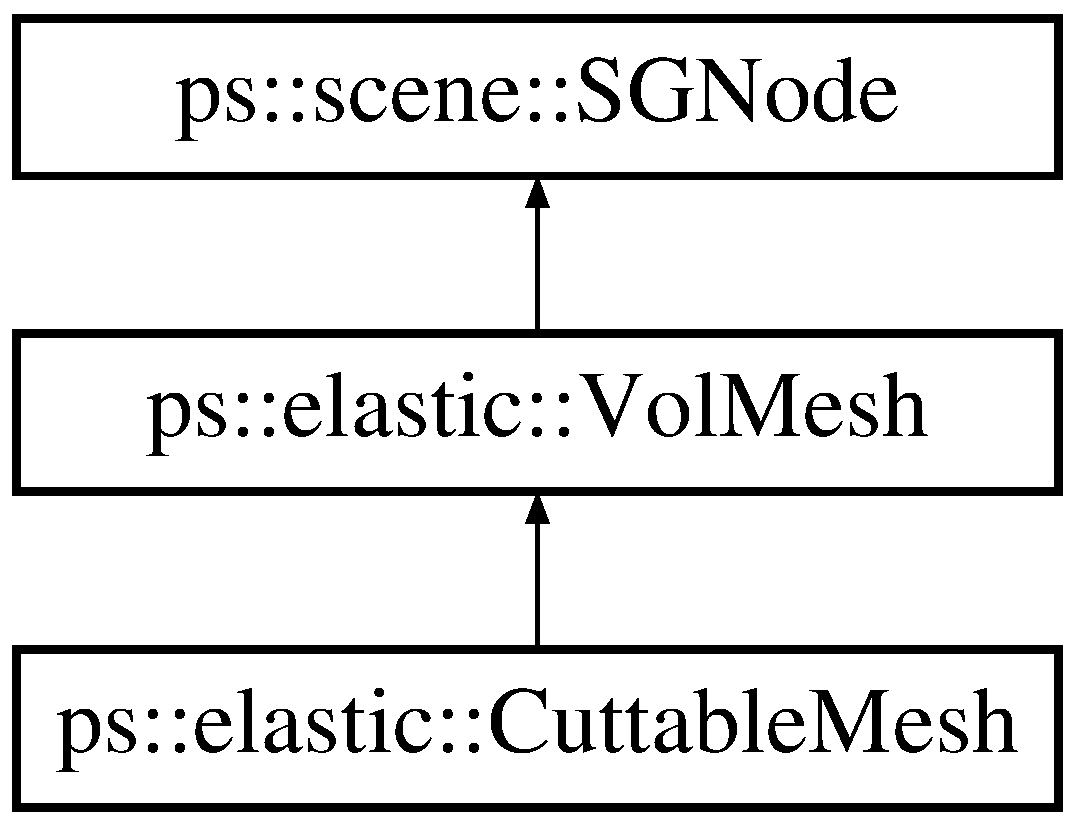
\includegraphics[height=3.000000cm]{classps_1_1elastic_1_1VolMesh}
\end{center}
\end{figure}
\subsection*{Public Types}
\begin{DoxyCompactItemize}
\item 
\hypertarget{classps_1_1elastic_1_1VolMesh_a8010471b44f64a1fe41ed63ff34a8305}{}enum {\bfseries Topology\+Event} \{ {\bfseries te\+Added}, 
{\bfseries te\+Removed}, 
{\bfseries te\+Updated}
 \}\label{classps_1_1elastic_1_1VolMesh_a8010471b44f64a1fe41ed63ff34a8305}

\item 
\hypertarget{classps_1_1elastic_1_1VolMesh_ae90aa791da6481aa8dc6ec612c2c3d49}{}enum {\bfseries Error\+Codes} \{ \\*
{\bfseries err\+\_\+op\+\_\+failed} = -\/1, 
{\bfseries err\+\_\+elem\+\_\+not\+\_\+found} = -\/2, 
{\bfseries err\+\_\+face\+\_\+not\+\_\+found} = -\/3, 
{\bfseries err\+\_\+edge\+\_\+not\+\_\+found} = -\/4, 
\\*
{\bfseries err\+\_\+node\+\_\+not\+\_\+found} = -\/5
 \}\label{classps_1_1elastic_1_1VolMesh_ae90aa791da6481aa8dc6ec612c2c3d49}

\item 
\hypertarget{classps_1_1elastic_1_1VolMesh_a2f2e69c7d7143e28ffcc4e06d90eda64}{}typedef std\+::function$<$ void(\hyperlink{classps_1_1elastic_1_1NODE}{N\+O\+D\+E}, U32 handle, Topology\+Event event)$>$ {\bfseries On\+Node\+Event}\label{classps_1_1elastic_1_1VolMesh_a2f2e69c7d7143e28ffcc4e06d90eda64}

\item 
\hypertarget{classps_1_1elastic_1_1VolMesh_addf9d9903c724cee6cd52e91fa5eeab2}{}typedef std\+::function$<$ void(\hyperlink{classps_1_1elastic_1_1EDGE}{E\+D\+G\+E}, U32 handle, Topology\+Event event)$>$ {\bfseries On\+Edge\+Event}\label{classps_1_1elastic_1_1VolMesh_addf9d9903c724cee6cd52e91fa5eeab2}

\item 
\hypertarget{classps_1_1elastic_1_1VolMesh_ac159aebf39215c8db149130b0bc2dd4d}{}typedef std\+::function$<$ void(\hyperlink{classps_1_1elastic_1_1FACE}{F\+A\+C\+E}, U32 handle, Topology\+Event event)$>$ {\bfseries On\+Face\+Event}\label{classps_1_1elastic_1_1VolMesh_ac159aebf39215c8db149130b0bc2dd4d}

\item 
\hypertarget{classps_1_1elastic_1_1VolMesh_a32e38574a3f9c8aa259669becffb689d}{}typedef std\+::function$<$ void(\hyperlink{classps_1_1elastic_1_1CELL}{C\+E\+L\+L}, U32 handle, Topology\+Event event)$>$ {\bfseries On\+Cell\+Event}\label{classps_1_1elastic_1_1VolMesh_a32e38574a3f9c8aa259669becffb689d}

\end{DoxyCompactItemize}
\subsection*{Public Member Functions}
\begin{DoxyCompactItemize}
\item 
\hypertarget{classps_1_1elastic_1_1VolMesh_ae6c4090f52d629275bafec3b28b82a72}{}{\bfseries Vol\+Mesh} (const \hyperlink{classps_1_1elastic_1_1VolMesh}{Vol\+Mesh} \&other)\label{classps_1_1elastic_1_1VolMesh_ae6c4090f52d629275bafec3b28b82a72}

\item 
\hypertarget{classps_1_1elastic_1_1VolMesh_a47f2518a104c2fd21038fd6293c5df4b}{}{\bfseries Vol\+Mesh} (U32 ct\+Vertices, double $\ast$vertices, U32 ct\+Elements, U32 $\ast$elements)\label{classps_1_1elastic_1_1VolMesh_a47f2518a104c2fd21038fd6293c5df4b}

\item 
\hypertarget{classps_1_1elastic_1_1VolMesh_a5d354fc8ecc1cf49eaabf54d47ffaf4f}{}{\bfseries Vol\+Mesh} (const vector$<$ double $>$ \&vertices, const vector$<$ U32 $>$ \&elements)\label{classps_1_1elastic_1_1VolMesh_a5d354fc8ecc1cf49eaabf54d47ffaf4f}

\item 
\hypertarget{classps_1_1elastic_1_1VolMesh_ae7e26e6519d1e2db5d5bbf58cb402906}{}void {\bfseries set\+On\+Node\+Event\+Callback} (On\+Node\+Event f)\label{classps_1_1elastic_1_1VolMesh_ae7e26e6519d1e2db5d5bbf58cb402906}

\item 
\hypertarget{classps_1_1elastic_1_1VolMesh_a38dde82b129ee0361b07162da7f9b60b}{}void {\bfseries set\+On\+Edge\+Event\+Callback} (On\+Edge\+Event f)\label{classps_1_1elastic_1_1VolMesh_a38dde82b129ee0361b07162da7f9b60b}

\item 
\hypertarget{classps_1_1elastic_1_1VolMesh_a96b1b84565c4c6b0224cc4d9ad738c90}{}void {\bfseries set\+On\+Face\+Event\+Callback} (On\+Face\+Event f)\label{classps_1_1elastic_1_1VolMesh_a96b1b84565c4c6b0224cc4d9ad738c90}

\item 
\hypertarget{classps_1_1elastic_1_1VolMesh_a4a72cb08f525cc838b474add44cb253b}{}void {\bfseries set\+On\+Elem\+Event\+Callback} (On\+Cell\+Event f)\label{classps_1_1elastic_1_1VolMesh_a4a72cb08f525cc838b474add44cb253b}

\item 
\hypertarget{classps_1_1elastic_1_1VolMesh_af0f695203df44322ab5d064d5b6f8b7e}{}bool {\bfseries setup} (const vector$<$ double $>$ \&vertices, const vector$<$ U32 $>$ \&elements)\label{classps_1_1elastic_1_1VolMesh_af0f695203df44322ab5d064d5b6f8b7e}

\item 
\hypertarget{classps_1_1elastic_1_1VolMesh_a22ec69f1fafb6470f4c86077aa785edc}{}bool {\bfseries setup} (U32 ct\+Vertices, const double $\ast$vertices, U32 ct\+Elements, const U32 $\ast$elements)\label{classps_1_1elastic_1_1VolMesh_a22ec69f1fafb6470f4c86077aa785edc}

\item 
\hypertarget{classps_1_1elastic_1_1VolMesh_ab5e7fad7fda1a51dc0e4f304dd4aa0ce}{}void {\bfseries cleanup} ()\label{classps_1_1elastic_1_1VolMesh_ab5e7fad7fda1a51dc0e4f304dd4aa0ce}

\item 
\hypertarget{classps_1_1elastic_1_1VolMesh_af749229a655b38582d9028c3cfbf394d}{}void {\bfseries print\+Node\+Info} () const \label{classps_1_1elastic_1_1VolMesh_af749229a655b38582d9028c3cfbf394d}

\item 
\hypertarget{classps_1_1elastic_1_1VolMesh_a32ca6c1d68d66f6cb1bde8f753ef24c1}{}void {\bfseries print\+Edge\+Info} () const \label{classps_1_1elastic_1_1VolMesh_a32ca6c1d68d66f6cb1bde8f753ef24c1}

\item 
\hypertarget{classps_1_1elastic_1_1VolMesh_ad22385def9a3182c478ea67c8ae85f37}{}void {\bfseries print\+Face\+Info} () const \label{classps_1_1elastic_1_1VolMesh_ad22385def9a3182c478ea67c8ae85f37}

\item 
\hypertarget{classps_1_1elastic_1_1VolMesh_a8ea54db807acc94c891ef91a677d0a00}{}void {\bfseries print\+Cell\+Info} () const \label{classps_1_1elastic_1_1VolMesh_a8ea54db807acc94c891ef91a677d0a00}

\item 
\hypertarget{classps_1_1elastic_1_1VolMesh_a75d8e756fdd5fcb664e352562ed37082}{}void {\bfseries print\+Info} () const \label{classps_1_1elastic_1_1VolMesh_a75d8e756fdd5fcb664e352562ed37082}

\item 
\hypertarget{classps_1_1elastic_1_1VolMesh_a8d8067f52b058c47f562362b030683e4}{}double {\bfseries compute\+Cell\+Determinant} (U32 idx\+Cell) const \label{classps_1_1elastic_1_1VolMesh_a8d8067f52b058c47f562362b030683e4}

\item 
\hypertarget{classps_1_1elastic_1_1VolMesh_a2322935cc39ca160d81afc85a07bb33d}{}double {\bfseries compute\+Cell\+Volume} (U32 idx\+Cell) const \label{classps_1_1elastic_1_1VolMesh_a2322935cc39ca160d81afc85a07bb33d}

\item 
\hypertarget{classps_1_1elastic_1_1VolMesh_af88b84f3c6a36015fd4d1b5b60a4f4b4}{}\hyperlink{classps_1_1base_1_1Vec3}{vec3d} {\bfseries compute\+Cell\+Centroid} (U32 idx\+Cell) const \label{classps_1_1elastic_1_1VolMesh_af88b84f3c6a36015fd4d1b5b60a4f4b4}

\item 
\hypertarget{classps_1_1elastic_1_1VolMesh_a799683f49aec6c0e6e70bc68f5e8a0b0}{}double {\bfseries compute\+Aspect\+Ratio} (U32 idx\+Cell) const \label{classps_1_1elastic_1_1VolMesh_a799683f49aec6c0e6e70bc68f5e8a0b0}

\item 
\hypertarget{classps_1_1elastic_1_1VolMesh_a1194410e557361559a0eb7ebde0270ee}{}double {\bfseries compute\+Inscribed\+Radius} (U32 idx\+Cell) const \label{classps_1_1elastic_1_1VolMesh_a1194410e557361559a0eb7ebde0270ee}

\item 
\hypertarget{classps_1_1elastic_1_1VolMesh_a9fdeddee8f948341861529a085be4299}{}double {\bfseries compute\+Circumscribed\+Radius} (U32 idx\+Cell) const \label{classps_1_1elastic_1_1VolMesh_a9fdeddee8f948341861529a085be4299}

\item 
\hypertarget{classps_1_1elastic_1_1VolMesh_a5f67ac6f5c6f41fb6e5725f34b94a333}{}U32 {\bfseries remove\+Zero\+Volume\+Cells} ()\label{classps_1_1elastic_1_1VolMesh_a5f67ac6f5c6f41fb6e5725f34b94a333}

\item 
\hypertarget{classps_1_1elastic_1_1VolMesh_adaf7ed1e46557f71b6d0c48c135303ff}{}bool {\bfseries is\+Cell\+Index} (U32 i) const \label{classps_1_1elastic_1_1VolMesh_adaf7ed1e46557f71b6d0c48c135303ff}

\item 
\hypertarget{classps_1_1elastic_1_1VolMesh_a24b73ef10efd1651eecf0a3431007083}{}bool {\bfseries is\+Face\+Index} (U32 i) const \label{classps_1_1elastic_1_1VolMesh_a24b73ef10efd1651eecf0a3431007083}

\item 
\hypertarget{classps_1_1elastic_1_1VolMesh_ae6d58ecf7f59e28da21b6eeb4b0afc57}{}bool {\bfseries is\+Edge\+Index} (U32 i) const \label{classps_1_1elastic_1_1VolMesh_ae6d58ecf7f59e28da21b6eeb4b0afc57}

\item 
\hypertarget{classps_1_1elastic_1_1VolMesh_acd4c370c20e0ab70e70439dac1ecb1e0}{}bool {\bfseries is\+Node\+Index} (U32 i) const \label{classps_1_1elastic_1_1VolMesh_acd4c370c20e0ab70e70439dac1ecb1e0}

\item 
\hypertarget{classps_1_1elastic_1_1VolMesh_ac7d3a6447c0c5eba8dcd829139bbc5f3}{}bool {\bfseries get\+Face\+Nodes} (U32 idx\+Face, U32(\&nodes)\mbox{[}3\mbox{]}) const \label{classps_1_1elastic_1_1VolMesh_ac7d3a6447c0c5eba8dcd829139bbc5f3}

\item 
\hypertarget{classps_1_1elastic_1_1VolMesh_a2cd4059bf1f21093e860e54fddb2d774}{}bool {\bfseries is\+Node\+Of\+Cell} (U32 idx\+Node, U32 idx\+Cell) const \label{classps_1_1elastic_1_1VolMesh_a2cd4059bf1f21093e860e54fddb2d774}

\item 
\hypertarget{classps_1_1elastic_1_1VolMesh_adf5932ab9ad4eeb93efb67d7b9f88fd4}{}bool {\bfseries is\+Edge\+Of\+Cell} (U32 idx\+Edge, U32 idx\+Cell) const \label{classps_1_1elastic_1_1VolMesh_adf5932ab9ad4eeb93efb67d7b9f88fd4}

\item 
\hypertarget{classps_1_1elastic_1_1VolMesh_a7d6a48de77e1687a75a2eab90b14437b}{}\hyperlink{classps_1_1elastic_1_1CELL}{C\+E\+L\+L} \& {\bfseries cell\+At} (U32 i)\label{classps_1_1elastic_1_1VolMesh_a7d6a48de77e1687a75a2eab90b14437b}

\item 
\hypertarget{classps_1_1elastic_1_1VolMesh_a7376563ee2f5887b9abe72a6afc2a188}{}\hyperlink{classps_1_1elastic_1_1FACE}{F\+A\+C\+E} \& {\bfseries face\+At} (U32 i)\label{classps_1_1elastic_1_1VolMesh_a7376563ee2f5887b9abe72a6afc2a188}

\item 
\hypertarget{classps_1_1elastic_1_1VolMesh_aeefd7f308c72b311d72c90b9e727a881}{}\hyperlink{classps_1_1elastic_1_1NODE}{N\+O\+D\+E} \& {\bfseries node\+At} (U32 i)\label{classps_1_1elastic_1_1VolMesh_aeefd7f308c72b311d72c90b9e727a881}

\item 
\hypertarget{classps_1_1elastic_1_1VolMesh_a21aadad5b2eb050b15f7b888cd577a00}{}\hyperlink{classps_1_1elastic_1_1EDGE}{E\+D\+G\+E} \& {\bfseries edge\+At} (U32 i)\label{classps_1_1elastic_1_1VolMesh_a21aadad5b2eb050b15f7b888cd577a00}

\item 
\hypertarget{classps_1_1elastic_1_1VolMesh_a8137affa13e3d75ed81c4045ae217b46}{}const \hyperlink{classps_1_1elastic_1_1CELL}{C\+E\+L\+L} \& {\bfseries const\+\_\+cell\+At\+\_\+} (const \hyperlink{classps_1_1elastic_1_1CellLink}{Cell\+Link} \&i) const \label{classps_1_1elastic_1_1VolMesh_a8137affa13e3d75ed81c4045ae217b46}

\item 
\hypertarget{classps_1_1elastic_1_1VolMesh_ace864f6a203698245debe23200074416}{}const \hyperlink{classps_1_1elastic_1_1CELL}{C\+E\+L\+L} \& {\bfseries const\+\_\+cell\+At} (U32 i) const \label{classps_1_1elastic_1_1VolMesh_ace864f6a203698245debe23200074416}

\item 
\hypertarget{classps_1_1elastic_1_1VolMesh_a719c366ad18b765f99101f162e4f8bc6}{}const \hyperlink{classps_1_1elastic_1_1FACE}{F\+A\+C\+E} \& {\bfseries const\+\_\+face\+At} (U32 i) const \label{classps_1_1elastic_1_1VolMesh_a719c366ad18b765f99101f162e4f8bc6}

\item 
\hypertarget{classps_1_1elastic_1_1VolMesh_ac94ac2764ce91974d76cd8cd77aea98c}{}const \hyperlink{classps_1_1elastic_1_1NODE}{N\+O\+D\+E} \& {\bfseries const\+\_\+node\+At} (U32 i) const \label{classps_1_1elastic_1_1VolMesh_ac94ac2764ce91974d76cd8cd77aea98c}

\item 
\hypertarget{classps_1_1elastic_1_1VolMesh_a27f8c12d7d11316183814e769f51bb86}{}const \hyperlink{classps_1_1elastic_1_1EDGE}{E\+D\+G\+E} \& {\bfseries const\+\_\+edge\+At} (U32 i) const \label{classps_1_1elastic_1_1VolMesh_a27f8c12d7d11316183814e769f51bb86}

\item 
\hypertarget{classps_1_1elastic_1_1VolMesh_a5dc6de26ea5b4ebc87628102cad24e0b}{}U32 {\bfseries count\+Cells} () const \label{classps_1_1elastic_1_1VolMesh_a5dc6de26ea5b4ebc87628102cad24e0b}

\item 
\hypertarget{classps_1_1elastic_1_1VolMesh_a4f3d740a8230a435a7a106db1fe5bd36}{}U32 {\bfseries count\+Faces} () const \label{classps_1_1elastic_1_1VolMesh_a4f3d740a8230a435a7a106db1fe5bd36}

\item 
\hypertarget{classps_1_1elastic_1_1VolMesh_a25b7d0c9ce6b0548eee74ed91f818ac8}{}U32 {\bfseries count\+Edges} () const \label{classps_1_1elastic_1_1VolMesh_a25b7d0c9ce6b0548eee74ed91f818ac8}

\item 
\hypertarget{classps_1_1elastic_1_1VolMesh_a9fa32f9e91357742d46a26904905ff00}{}U32 {\bfseries count\+Nodes} () const \label{classps_1_1elastic_1_1VolMesh_a9fa32f9e91357742d46a26904905ff00}

\item 
\hypertarget{classps_1_1elastic_1_1VolMesh_a3563d3a1ad60de33565059eec9d31fd0}{}U32 {\bfseries count\+Incident\+Cells} (U32 idx\+Face) const \label{classps_1_1elastic_1_1VolMesh_a3563d3a1ad60de33565059eec9d31fd0}

\item 
\hypertarget{classps_1_1elastic_1_1VolMesh_a8952131069dcf8c966e0d257708a8679}{}U32 {\bfseries count\+Incident\+Faces} (U32 idx\+Edge) const \label{classps_1_1elastic_1_1VolMesh_a8952131069dcf8c966e0d257708a8679}

\item 
\hypertarget{classps_1_1elastic_1_1VolMesh_a7caf2554abe121c2afb761facc784364}{}U32 {\bfseries count\+Incident\+Edges} (U32 idx\+Node) const \label{classps_1_1elastic_1_1VolMesh_a7caf2554abe121c2afb761facc784364}

\item 
\hypertarget{classps_1_1elastic_1_1VolMesh_ae9f65f3caa6d8079dd2af8f87e165fa0}{}bool {\bfseries edge\+\_\+exists} (U32 from, U32 to)\label{classps_1_1elastic_1_1VolMesh_ae9f65f3caa6d8079dd2af8f87e165fa0}

\item 
\hypertarget{classps_1_1elastic_1_1VolMesh_a81b08888ae16c8bfc6e0a600045911a6}{}U32 {\bfseries edge\+\_\+handle} (U32 from, U32 to)\label{classps_1_1elastic_1_1VolMesh_a81b08888ae16c8bfc6e0a600045911a6}

\item 
\hypertarget{classps_1_1elastic_1_1VolMesh_a693b256705ed37a34c376a6d8ee64077}{}U32 {\bfseries edge\+\_\+from\+\_\+node} (U32 idx\+Edge) const \label{classps_1_1elastic_1_1VolMesh_a693b256705ed37a34c376a6d8ee64077}

\item 
\hypertarget{classps_1_1elastic_1_1VolMesh_a44b29ea290f6ccde40c9915a332194c2}{}U32 {\bfseries edge\+\_\+to\+\_\+node} (U32 idx\+Edge) const \label{classps_1_1elastic_1_1VolMesh_a44b29ea290f6ccde40c9915a332194c2}

\item 
\hypertarget{classps_1_1elastic_1_1VolMesh_af388dbb76bd8a002001dfb6ed84cb9b3}{}U32 {\bfseries get\+\_\+node\+\_\+neighbors} (U32 idx\+Node, vector$<$ U32 $>$ \&nbors) const \label{classps_1_1elastic_1_1VolMesh_af388dbb76bd8a002001dfb6ed84cb9b3}

\item 
\hypertarget{classps_1_1elastic_1_1VolMesh_ab089dca62b3a7fe26f925d9fe3dd6672}{}void {\bfseries displace} (U32 count\+Degrees\+Of\+Freedom, const double $\ast$u)\label{classps_1_1elastic_1_1VolMesh_ab089dca62b3a7fe26f925d9fe3dd6672}

\item 
\hypertarget{classps_1_1elastic_1_1VolMesh_a02cf4f39e82f844d1280245e1ebcab83}{}U32 {\bfseries insert\+\_\+node} (const \hyperlink{classps_1_1elastic_1_1NODE}{N\+O\+D\+E} \&n)\label{classps_1_1elastic_1_1VolMesh_a02cf4f39e82f844d1280245e1ebcab83}

\item 
\hypertarget{classps_1_1elastic_1_1VolMesh_a5d73955fe15e4e1311ba58d7de64bc14}{}U32 {\bfseries insert\+\_\+edge} (const \hyperlink{classps_1_1elastic_1_1EDGE}{E\+D\+G\+E} \&e)\label{classps_1_1elastic_1_1VolMesh_a5d73955fe15e4e1311ba58d7de64bc14}

\item 
\hypertarget{classps_1_1elastic_1_1VolMesh_a48b3ba9227d5bb8734007d30e69fa254}{}U32 {\bfseries insert\+\_\+face} (U32 nodes\mbox{[}3\mbox{]})\label{classps_1_1elastic_1_1VolMesh_a48b3ba9227d5bb8734007d30e69fa254}

\item 
\hypertarget{classps_1_1elastic_1_1VolMesh_a62787fea4fe6e77eaf880a51c6ae50e2}{}bool {\bfseries insert\+\_\+cell} (const \hyperlink{classps_1_1elastic_1_1CELL}{C\+E\+L\+L} \&cell)\label{classps_1_1elastic_1_1VolMesh_a62787fea4fe6e77eaf880a51c6ae50e2}

\item 
\hypertarget{classps_1_1elastic_1_1VolMesh_ac875d4e69c1367bb9af3bb0de67141a5}{}bool {\bfseries insert\+\_\+cell} (U32 nodes\mbox{[}4\mbox{]})\label{classps_1_1elastic_1_1VolMesh_ac875d4e69c1367bb9af3bb0de67141a5}

\item 
\hypertarget{classps_1_1elastic_1_1VolMesh_a8677786b8f15d5012a2a5c8cf5c99e73}{}void {\bfseries set\+\_\+edge} (U32 idx\+Edge, U32 from, U32 to)\label{classps_1_1elastic_1_1VolMesh_a8677786b8f15d5012a2a5c8cf5c99e73}

\item 
\hypertarget{classps_1_1elastic_1_1VolMesh_ae6b152eca45ca7a1331345a1429b93a1}{}void {\bfseries set\+\_\+face} (U32 idx\+Face, U32 edges\mbox{[}3\mbox{]})\label{classps_1_1elastic_1_1VolMesh_ae6b152eca45ca7a1331345a1429b93a1}

\item 
\hypertarget{classps_1_1elastic_1_1VolMesh_a116c78d4b6e25d725c8ffa6346686f36}{}int {\bfseries get\+\_\+disjoint\+\_\+parts} (vector$<$ vector$<$ U32 $>$$>$ \&cellgroups)\label{classps_1_1elastic_1_1VolMesh_a116c78d4b6e25d725c8ffa6346686f36}

\item 
\hypertarget{classps_1_1elastic_1_1VolMesh_a738d968a386c0f098d9f080d1b508306}{}void {\bfseries print\+Parts} ()\label{classps_1_1elastic_1_1VolMesh_a738d968a386c0f098d9f080d1b508306}

\item 
\hypertarget{classps_1_1elastic_1_1VolMesh_ad1320533258c88bc9bbd92c019e1872f}{}void {\bfseries schedule\+\_\+remove\+\_\+cell} (U32 idx\+Cell)\label{classps_1_1elastic_1_1VolMesh_ad1320533258c88bc9bbd92c019e1872f}

\item 
\hypertarget{classps_1_1elastic_1_1VolMesh_aa9d69b01b41d133ff7f3041fc9c05ece}{}void {\bfseries remove\+\_\+cell} (U32 idx\+Cell)\label{classps_1_1elastic_1_1VolMesh_aa9d69b01b41d133ff7f3041fc9c05ece}

\item 
\hypertarget{classps_1_1elastic_1_1VolMesh_a263a2a1505154aaa2bb2ebce3b50dc98}{}void {\bfseries remove\+\_\+face} (U32 idx\+Face)\label{classps_1_1elastic_1_1VolMesh_a263a2a1505154aaa2bb2ebce3b50dc98}

\item 
\hypertarget{classps_1_1elastic_1_1VolMesh_afdd3edf9cb3474951122beec3896f7d2}{}void {\bfseries remove\+\_\+edge} (U32 idx\+Edge)\label{classps_1_1elastic_1_1VolMesh_afdd3edf9cb3474951122beec3896f7d2}

\item 
\hypertarget{classps_1_1elastic_1_1VolMesh_a4f5b66732b5343ac3845e6638b557491}{}void {\bfseries remove\+\_\+node} (U32 idx\+Node)\label{classps_1_1elastic_1_1VolMesh_a4f5b66732b5343ac3845e6638b557491}

\item 
\hypertarget{classps_1_1elastic_1_1VolMesh_ab165c26790cfc1a4e2260ccecae93ff0}{}{\footnotesize template$<$class Container\+T $>$ }\\void {\bfseries remove\+\_\+cells} (const Container\+T \&cells)\label{classps_1_1elastic_1_1VolMesh_ab165c26790cfc1a4e2260ccecae93ff0}

\item 
\hypertarget{classps_1_1elastic_1_1VolMesh_ac42ae75f8d206a2f483c8a268cf98c8b}{}{\footnotesize template$<$class Container\+T $>$ }\\void {\bfseries remove\+\_\+faces} (const Container\+T \&faces)\label{classps_1_1elastic_1_1VolMesh_ac42ae75f8d206a2f483c8a268cf98c8b}

\item 
\hypertarget{classps_1_1elastic_1_1VolMesh_a8929becd264cb9ded00c74c536a8cf26}{}{\footnotesize template$<$class Container\+T $>$ }\\void {\bfseries remove\+\_\+edges} (const Container\+T \&edges)\label{classps_1_1elastic_1_1VolMesh_a8929becd264cb9ded00c74c536a8cf26}

\item 
\hypertarget{classps_1_1elastic_1_1VolMesh_af8aae2ff9d1031e8d4306bd4cdce9e82}{}{\footnotesize template$<$class Container\+T $>$ }\\void {\bfseries remove\+\_\+nodes} (const Container\+T \&nodes)\label{classps_1_1elastic_1_1VolMesh_af8aae2ff9d1031e8d4306bd4cdce9e82}

\item 
\hypertarget{classps_1_1elastic_1_1VolMesh_a9c540723cbf4c7bea9af0f45ab84ee68}{}void {\bfseries garbage\+\_\+collection} ()\label{classps_1_1elastic_1_1VolMesh_a9c540723cbf4c7bea9af0f45ab84ee68}

\item 
bool \hyperlink{classps_1_1elastic_1_1VolMesh_a842ed44f9368421b32524b057cee2b58}{cut\+\_\+edge} (int idx\+Edge, double distance, U32 $\ast$pout\+Index\+N\+P0=N\+U\+L\+L, U32 $\ast$pout\+Index\+N\+P1=N\+U\+L\+L)
\item 
\hypertarget{classps_1_1elastic_1_1VolMesh_a9f2ddb6b25e1b608fb7ff37dbcf71009}{}int {\bfseries get\+Node\+Incident\+Edges} (U32 idx\+Node, vector$<$ U32 $>$ \&incident\+Edges) const \label{classps_1_1elastic_1_1VolMesh_a9f2ddb6b25e1b608fb7ff37dbcf71009}

\item 
\hypertarget{classps_1_1elastic_1_1VolMesh_a3bbd2d1170bca105b0bed88d4023e795}{}int {\bfseries get\+Node\+Incident\+Nodes} (U32 idx\+Node, vector$<$ U32 $>$ \&incident\+Nodes) const \label{classps_1_1elastic_1_1VolMesh_a3bbd2d1170bca105b0bed88d4023e795}

\item 
\hypertarget{classps_1_1elastic_1_1VolMesh_a1c77dd15d2adc50e1c63507e7369880f}{}bool {\bfseries get\+Cell\+Faces\+Expensive} (U32 idx\+Cell, U32(\&faces)\mbox{[}4\mbox{]})\label{classps_1_1elastic_1_1VolMesh_a1c77dd15d2adc50e1c63507e7369880f}

\item 
\hypertarget{classps_1_1elastic_1_1VolMesh_a656608a0c79e22cc0735d0060e0da3e1}{}bool {\bfseries get\+Cell\+Edges\+Expensive} (U32 idx\+Cell, U32(\&edges)\mbox{[}6\mbox{]})\label{classps_1_1elastic_1_1VolMesh_a656608a0c79e22cc0735d0060e0da3e1}

\item 
\hypertarget{classps_1_1elastic_1_1VolMesh_a3f90d8aaf6d2a78dc795c64e14f5f251}{}void {\bfseries set\+Elem\+To\+Show} (U32 elem=I\+N\+V\+A\+L\+I\+D\+\_\+\+I\+N\+D\+E\+X)\label{classps_1_1elastic_1_1VolMesh_a3f90d8aaf6d2a78dc795c64e14f5f251}

\item 
\hypertarget{classps_1_1elastic_1_1VolMesh_a6afa5a0a0d179a42bd92b7fc6abfd4c1}{}U32 {\bfseries get\+Elem\+To\+Show} () const \label{classps_1_1elastic_1_1VolMesh_a6afa5a0a0d179a42bd92b7fc6abfd4c1}

\item 
\hypertarget{classps_1_1elastic_1_1VolMesh_ae423b20d80615e4c48b14133ac06b4c7}{}void {\bfseries set\+Node\+To\+Show} (U32 idx\+Node=I\+N\+V\+A\+L\+I\+D\+\_\+\+I\+N\+D\+E\+X)\label{classps_1_1elastic_1_1VolMesh_ae423b20d80615e4c48b14133ac06b4c7}

\item 
\hypertarget{classps_1_1elastic_1_1VolMesh_aebd1d9e8d715d747218bc82f05d2beac}{}U32 {\bfseries get\+Node\+To\+Show} () const \label{classps_1_1elastic_1_1VolMesh_aebd1d9e8d715d747218bc82f05d2beac}

\item 
\hypertarget{classps_1_1elastic_1_1VolMesh_adb03f406b1622d57049b4e83194cab50}{}void {\bfseries set\+Flag\+Draw\+Wire\+Frame} (bool draw\+Wire\+Frame)\label{classps_1_1elastic_1_1VolMesh_adb03f406b1622d57049b4e83194cab50}

\item 
\hypertarget{classps_1_1elastic_1_1VolMesh_a8c3fde2f947e739db79303cf1bb373fb}{}bool {\bfseries get\+Flag\+Draw\+Wire\+Frame} () const \label{classps_1_1elastic_1_1VolMesh_a8c3fde2f947e739db79303cf1bb373fb}

\item 
\hypertarget{classps_1_1elastic_1_1VolMesh_af7d3b4ce18468c34cee2744313f9f7f3}{}void {\bfseries set\+Flag\+Draw\+Nodes} (bool draw\+Nodes)\label{classps_1_1elastic_1_1VolMesh_af7d3b4ce18468c34cee2744313f9f7f3}

\item 
\hypertarget{classps_1_1elastic_1_1VolMesh_a4b6d0d1392097bb3614942ad31ad9db5}{}bool {\bfseries get\+Flag\+Draw\+Nodes} () const \label{classps_1_1elastic_1_1VolMesh_a4b6d0d1392097bb3614942ad31ad9db5}

\item 
\hypertarget{classps_1_1elastic_1_1VolMesh_ac1b42580f896ad58c076e0a326ff38a4}{}void {\bfseries set\+Flag\+Filter\+Out\+Flat\+Cells} (bool flag)\label{classps_1_1elastic_1_1VolMesh_ac1b42580f896ad58c076e0a326ff38a4}

\item 
\hypertarget{classps_1_1elastic_1_1VolMesh_a649a2c0ee8725e248383b2db9b763e31}{}bool {\bfseries get\+Flag\+Filter\+Out\+Flat\+Cells} () const \label{classps_1_1elastic_1_1VolMesh_a649a2c0ee8725e248383b2db9b763e31}

\item 
\hypertarget{classps_1_1elastic_1_1VolMesh_a5970a04c412bad03c25486514fef2dc1}{}\hyperlink{classps_1_1base_1_1Color}{Color} {\bfseries get\+Color} () const \label{classps_1_1elastic_1_1VolMesh_a5970a04c412bad03c25486514fef2dc1}

\item 
\hypertarget{classps_1_1elastic_1_1VolMesh_aeb013656c4952cf4351e1f0303dae8a4}{}void {\bfseries set\+Color} (const \hyperlink{classps_1_1base_1_1Color}{Color} \&c)\label{classps_1_1elastic_1_1VolMesh_aeb013656c4952cf4351e1f0303dae8a4}

\item 
\hypertarget{classps_1_1elastic_1_1VolMesh_ad8e58758dc76e01c9a92d45fec545a09}{}void {\bfseries draw} ()\label{classps_1_1elastic_1_1VolMesh_ad8e58758dc76e01c9a92d45fec545a09}

\item 
\hypertarget{classps_1_1elastic_1_1VolMesh_aa8b6f71abb3b6e7a0cff29ac22ada02a}{}void {\bfseries draw\+Element} (U32 i) const \label{classps_1_1elastic_1_1VolMesh_aa8b6f71abb3b6e7a0cff29ac22ada02a}

\item 
\hypertarget{classps_1_1elastic_1_1VolMesh_a40bedb0cb685045f536fe523eac8f7a3}{}\hyperlink{classps_1_1base_1_1AABB}{A\+A\+B\+B} {\bfseries compute\+A\+A\+B\+B} ()\label{classps_1_1elastic_1_1VolMesh_a40bedb0cb685045f536fe523eac8f7a3}

\item 
\hypertarget{classps_1_1elastic_1_1VolMesh_a97ff3111e9d6cb683f5ebce64abc84bf}{}int {\bfseries select\+Node} (const \hyperlink{classps_1_1base_1_1Ray}{Ray} \&ray) const \label{classps_1_1elastic_1_1VolMesh_a97ff3111e9d6cb683f5ebce64abc84bf}

\item 
\hypertarget{classps_1_1elastic_1_1VolMesh_aa78fbef753134fb6b13962b5db60ae7b}{}bool {\bfseries verbose} () const \label{classps_1_1elastic_1_1VolMesh_aa78fbef753134fb6b13962b5db60ae7b}

\item 
\hypertarget{classps_1_1elastic_1_1VolMesh_a35ee920238424a53b34407dea46f6ab6}{}void {\bfseries set\+Verbose} (bool b)\label{classps_1_1elastic_1_1VolMesh_a35ee920238424a53b34407dea46f6ab6}

\end{DoxyCompactItemize}
\subsection*{Static Public Member Functions}
\begin{DoxyCompactItemize}
\item 
\hypertarget{classps_1_1elastic_1_1VolMesh_af2c0768be3acb734df082712d6dd70ce}{}static double {\bfseries Compute\+Circumscribed\+Radius} (const \hyperlink{classps_1_1base_1_1Vec3}{vec3d} v\mbox{[}4\mbox{]})\label{classps_1_1elastic_1_1VolMesh_af2c0768be3acb734df082712d6dd70ce}

\item 
\hypertarget{classps_1_1elastic_1_1VolMesh_a5ee3dad4afc9eeb54d890ea6462cb8e7}{}static double {\bfseries Compute\+Cell\+Determinant} (const \hyperlink{classps_1_1base_1_1Vec3}{vec3d} v\mbox{[}4\mbox{]})\label{classps_1_1elastic_1_1VolMesh_a5ee3dad4afc9eeb54d890ea6462cb8e7}

\item 
\hypertarget{classps_1_1elastic_1_1VolMesh_a790bef93bef6986d7d0e5e50a10bb348}{}static double {\bfseries Compute\+Cell\+Volume} (const \hyperlink{classps_1_1base_1_1Vec3}{vec3d} v\mbox{[}4\mbox{]})\label{classps_1_1elastic_1_1VolMesh_a790bef93bef6986d7d0e5e50a10bb348}

\end{DoxyCompactItemize}
\subsection*{Static Public Attributes}
\begin{DoxyCompactItemize}
\item 
\hypertarget{classps_1_1elastic_1_1VolMesh_a20f60f24dd56a38318528ddff20a91de}{}static const U32 {\bfseries I\+N\+V\+A\+L\+I\+D\+\_\+\+I\+N\+D\+E\+X} = -\/1\label{classps_1_1elastic_1_1VolMesh_a20f60f24dd56a38318528ddff20a91de}

\end{DoxyCompactItemize}
\subsection*{Protected Types}
\begin{DoxyCompactItemize}
\item 
\hypertarget{classps_1_1elastic_1_1VolMesh_aee7e3fe8936e4704c38aa7407bb0abf5}{}typedef std\+::map$<$ \hyperlink{classps_1_1elastic_1_1EdgeKey}{Edge\+Key}, U32 $>$\+::iterator {\bfseries M\+A\+P\+H\+E\+D\+G\+E\+I\+N\+D\+E\+X\+I\+T\+E\+R}\label{classps_1_1elastic_1_1VolMesh_aee7e3fe8936e4704c38aa7407bb0abf5}

\item 
\hypertarget{classps_1_1elastic_1_1VolMesh_ae1ecbb97b86bf07bd1a9cfe176b912d5}{}typedef std\+::map$<$ \hyperlink{classps_1_1elastic_1_1EdgeKey}{Edge\+Key}, U32 $>$\+::const\+\_\+iterator {\bfseries M\+A\+P\+H\+E\+D\+G\+E\+I\+N\+D\+E\+X\+C\+O\+N\+S\+T\+I\+T\+E\+R}\label{classps_1_1elastic_1_1VolMesh_ae1ecbb97b86bf07bd1a9cfe176b912d5}

\end{DoxyCompactItemize}
\subsection*{Protected Member Functions}
\begin{DoxyCompactItemize}
\item 
\hypertarget{classps_1_1elastic_1_1VolMesh_abb320bf8584333cca98e316b8d5ad27d}{}void {\bfseries init} ()\label{classps_1_1elastic_1_1VolMesh_abb320bf8584333cca98e316b8d5ad27d}

\item 
\hypertarget{classps_1_1elastic_1_1VolMesh_a759d2e1cf8ba362be411646bfabc389e}{}bool {\bfseries insert\+Edge\+Index\+To\+Map} (U32 from, U32 to, U32 idx\+Edge)\label{classps_1_1elastic_1_1VolMesh_a759d2e1cf8ba362be411646bfabc389e}

\item 
\hypertarget{classps_1_1elastic_1_1VolMesh_aed8c037e96e3874e05af24e49dfd2746}{}bool {\bfseries remove\+Edge\+Index\+From\+Map} (U32 from, U32 to)\label{classps_1_1elastic_1_1VolMesh_aed8c037e96e3874e05af24e49dfd2746}

\item 
\hypertarget{classps_1_1elastic_1_1VolMesh_a277fde736ee27c4b6f8fdfbade377b77}{}\hyperlink{classps_1_1elastic_1_1EdgeKey}{Edge\+Key} {\bfseries compute\+Edge\+Key} (U32 idx\+Edge) const \label{classps_1_1elastic_1_1VolMesh_a277fde736ee27c4b6f8fdfbade377b77}

\item 
\hypertarget{classps_1_1elastic_1_1VolMesh_ae49c6f62434562e514c8c7b2bfe222d8}{}bool {\bfseries face\+\_\+exists\+\_\+by\+\_\+edges} (U32 edges\mbox{[}3\mbox{]}) const \label{classps_1_1elastic_1_1VolMesh_ae49c6f62434562e514c8c7b2bfe222d8}

\item 
\hypertarget{classps_1_1elastic_1_1VolMesh_a0203f03caae4eec5e116a23837090fe9}{}bool {\bfseries face\+\_\+exists\+\_\+by\+\_\+nodes} (U32 nodes\mbox{[}3\mbox{]})\label{classps_1_1elastic_1_1VolMesh_a0203f03caae4eec5e116a23837090fe9}

\item 
\hypertarget{classps_1_1elastic_1_1VolMesh_a4826f5ca02656c317bb5743885ec33ed}{}U32 {\bfseries face\+\_\+handle\+\_\+by\+\_\+edges} (U32 edges\mbox{[}3\mbox{]}) const \label{classps_1_1elastic_1_1VolMesh_a4826f5ca02656c317bb5743885ec33ed}

\item 
\hypertarget{classps_1_1elastic_1_1VolMesh_ae96ac686b704e333495b469874feabe0}{}U32 {\bfseries face\+\_\+handle\+\_\+by\+\_\+nodes} (U32 nodes\mbox{[}3\mbox{]})\label{classps_1_1elastic_1_1VolMesh_ae96ac686b704e333495b469874feabe0}

\item 
\hypertarget{classps_1_1elastic_1_1VolMesh_a7014b6c276e42bbeac0a9448ccf4d646}{}{\footnotesize template$<$class Container\+T $>$ }\\int {\bfseries get\+\_\+incident\+\_\+cells} (const Container\+T \&in\+\_\+faces, set$<$ U32 $>$ \&out\+\_\+cells) const \label{classps_1_1elastic_1_1VolMesh_a7014b6c276e42bbeac0a9448ccf4d646}

\item 
\hypertarget{classps_1_1elastic_1_1VolMesh_a179baac43bb17ed6649a97a24a6046ae}{}{\footnotesize template$<$class Container\+T $>$ }\\int {\bfseries get\+\_\+incident\+\_\+faces} (const Container\+T \&in\+\_\+edges, set$<$ U32 $>$ \&out\+\_\+faces) const \label{classps_1_1elastic_1_1VolMesh_a179baac43bb17ed6649a97a24a6046ae}

\item 
\hypertarget{classps_1_1elastic_1_1VolMesh_a9883a2d3dc5c6ff11a695ffd969c8c0d}{}{\footnotesize template$<$class Container\+T $>$ }\\int {\bfseries get\+\_\+incident\+\_\+edges} (const Container\+T \&in\+\_\+nodes, set$<$ U32 $>$ \&out\+\_\+edges) const \label{classps_1_1elastic_1_1VolMesh_a9883a2d3dc5c6ff11a695ffd969c8c0d}

\item 
\hypertarget{classps_1_1elastic_1_1VolMesh_ad0a4b9e354728e2f5a6f7b48e4b04bf5}{}bool {\bfseries test\+\_\+cell\+\_\+topology} (U32 idx\+Cell)\label{classps_1_1elastic_1_1VolMesh_ad0a4b9e354728e2f5a6f7b48e4b04bf5}

\item 
\hypertarget{classps_1_1elastic_1_1VolMesh_a86aa2fd8fe0b8549a686da18f1c8c3b9}{}bool {\bfseries test\+\_\+cells\+\_\+topology} ()\label{classps_1_1elastic_1_1VolMesh_a86aa2fd8fe0b8549a686da18f1c8c3b9}

\item 
\hypertarget{classps_1_1elastic_1_1VolMesh_aa752e76ab675865d94241d0331ae4afe}{}bool {\bfseries test\+\_\+incident\+\_\+edges} ()\label{classps_1_1elastic_1_1VolMesh_aa752e76ab675865d94241d0331ae4afe}

\item 
\hypertarget{classps_1_1elastic_1_1VolMesh_a455742cfc630ca08fb685f77c6ab6747}{}bool {\bfseries test\+\_\+incident\+\_\+faces} () const \label{classps_1_1elastic_1_1VolMesh_a455742cfc630ca08fb685f77c6ab6747}

\item 
\hypertarget{classps_1_1elastic_1_1VolMesh_a9bc4f2b019fd887cf021baab0b03e9b2}{}bool {\bfseries test\+\_\+incident\+\_\+cells} () const \label{classps_1_1elastic_1_1VolMesh_a9bc4f2b019fd887cf021baab0b03e9b2}

\item 
\hypertarget{classps_1_1elastic_1_1VolMesh_a157fd4f7bd24dcc94bf21b51a7286c9b}{}bool {\bfseries test\+\_\+incidents} ()\label{classps_1_1elastic_1_1VolMesh_a157fd4f7bd24dcc94bf21b51a7286c9b}

\item 
\hypertarget{classps_1_1elastic_1_1VolMesh_afdfce53c88c09bde6783aa5e79f291bf}{}\hyperlink{classps_1_1base_1_1AABB}{A\+A\+B\+B} {\bfseries compute\+Nodal\+A\+A\+B\+B} () const \label{classps_1_1elastic_1_1VolMesh_afdfce53c88c09bde6783aa5e79f291bf}

\item 
\hypertarget{classps_1_1elastic_1_1VolMesh_aa853df8d3a0435de40233469434eea69}{}void {\bfseries remove\+\_\+cell\+\_\+core} (U32 idx\+Cell)\label{classps_1_1elastic_1_1VolMesh_aa853df8d3a0435de40233469434eea69}

\item 
\hypertarget{classps_1_1elastic_1_1VolMesh_a04ea38a26a251e4baf8ad4d72da7bfa1}{}void {\bfseries remove\+\_\+face\+\_\+core} (U32 idx\+Face)\label{classps_1_1elastic_1_1VolMesh_a04ea38a26a251e4baf8ad4d72da7bfa1}

\item 
\hypertarget{classps_1_1elastic_1_1VolMesh_a29f4316ae30eb6758891d6e3cb74b771}{}void {\bfseries remove\+\_\+edge\+\_\+core} (U32 idx\+Edge)\label{classps_1_1elastic_1_1VolMesh_a29f4316ae30eb6758891d6e3cb74b771}

\item 
\hypertarget{classps_1_1elastic_1_1VolMesh_a9cd4febbd7cf8c10a34fd493ec4960a7}{}void {\bfseries remove\+\_\+node\+\_\+core} (U32 idx\+Node)\label{classps_1_1elastic_1_1VolMesh_a9cd4febbd7cf8c10a34fd493ec4960a7}

\end{DoxyCompactItemize}
\subsection*{Protected Attributes}
\begin{DoxyCompactItemize}
\item 
\hypertarget{classps_1_1elastic_1_1VolMesh_a9dd85ec6f1b3094de5e793a137d9e702}{}U32 {\bfseries m\+\_\+elem\+To\+Show}\label{classps_1_1elastic_1_1VolMesh_a9dd85ec6f1b3094de5e793a137d9e702}

\item 
\hypertarget{classps_1_1elastic_1_1VolMesh_a0894ac35582e8cb020093a5a70f363db}{}U32 {\bfseries m\+\_\+node\+To\+Show}\label{classps_1_1elastic_1_1VolMesh_a0894ac35582e8cb020093a5a70f363db}

\item 
\hypertarget{classps_1_1elastic_1_1VolMesh_a1ba86f2a9c19e73147d32d98c5503be4}{}bool {\bfseries m\+\_\+verbose}\label{classps_1_1elastic_1_1VolMesh_a1ba86f2a9c19e73147d32d98c5503be4}

\item 
\hypertarget{classps_1_1elastic_1_1VolMesh_a5dcd718e4185c4f47928062177e67676}{}bool {\bfseries m\+\_\+flag\+Draw\+Wire\+Frame\+Mesh}\label{classps_1_1elastic_1_1VolMesh_a5dcd718e4185c4f47928062177e67676}

\item 
\hypertarget{classps_1_1elastic_1_1VolMesh_a8a3cd08b75a8ade705cb8a9f1b401292}{}bool {\bfseries m\+\_\+flag\+Draw\+Nodes}\label{classps_1_1elastic_1_1VolMesh_a8a3cd08b75a8ade705cb8a9f1b401292}

\item 
\hypertarget{classps_1_1elastic_1_1VolMesh_afe59538f6681859cc18baf130688c7c1}{}bool {\bfseries m\+\_\+flag\+Filter\+Out\+Flat\+Cells}\label{classps_1_1elastic_1_1VolMesh_afe59538f6681859cc18baf130688c7c1}

\item 
\hypertarget{classps_1_1elastic_1_1VolMesh_a2a7c269ce78564a37885a9e3f5565650}{}\hyperlink{classps_1_1base_1_1Color}{Color} {\bfseries m\+\_\+color}\label{classps_1_1elastic_1_1VolMesh_a2a7c269ce78564a37885a9e3f5565650}

\item 
\hypertarget{classps_1_1elastic_1_1VolMesh_a7d352ef748521ced66e9ec007c82ad52}{}On\+Node\+Event {\bfseries m\+\_\+f\+On\+Node\+Event}\label{classps_1_1elastic_1_1VolMesh_a7d352ef748521ced66e9ec007c82ad52}

\item 
\hypertarget{classps_1_1elastic_1_1VolMesh_aae4b75ed2b6e579113facf9651cba55e}{}On\+Edge\+Event {\bfseries m\+\_\+f\+On\+Edge\+Event}\label{classps_1_1elastic_1_1VolMesh_aae4b75ed2b6e579113facf9651cba55e}

\item 
\hypertarget{classps_1_1elastic_1_1VolMesh_a2586742c1c69d289fb03a5760048a198}{}On\+Face\+Event {\bfseries m\+\_\+f\+On\+Face\+Event}\label{classps_1_1elastic_1_1VolMesh_a2586742c1c69d289fb03a5760048a198}

\item 
\hypertarget{classps_1_1elastic_1_1VolMesh_a147ceb73a33f31ca4205d7f74866b5ed}{}On\+Cell\+Event {\bfseries m\+\_\+f\+On\+Element\+Event}\label{classps_1_1elastic_1_1VolMesh_a147ceb73a33f31ca4205d7f74866b5ed}

\item 
\hypertarget{classps_1_1elastic_1_1VolMesh_a5055d98d4124c7f8fccbe503a2152354}{}vector$<$ \hyperlink{classps_1_1elastic_1_1CELL}{C\+E\+L\+L} $>$ {\bfseries m\+\_\+v\+Cells}\label{classps_1_1elastic_1_1VolMesh_a5055d98d4124c7f8fccbe503a2152354}

\item 
\hypertarget{classps_1_1elastic_1_1VolMesh_a466ed1e2d8ede1b420b48494e8394efa}{}vector$<$ \hyperlink{classps_1_1elastic_1_1FACE}{F\+A\+C\+E} $>$ {\bfseries m\+\_\+v\+Faces}\label{classps_1_1elastic_1_1VolMesh_a466ed1e2d8ede1b420b48494e8394efa}

\item 
\hypertarget{classps_1_1elastic_1_1VolMesh_a12f235278685485ee19a1961bd84ee71}{}vector$<$ \hyperlink{classps_1_1elastic_1_1EDGE}{E\+D\+G\+E} $>$ {\bfseries m\+\_\+v\+Edges}\label{classps_1_1elastic_1_1VolMesh_a12f235278685485ee19a1961bd84ee71}

\item 
\hypertarget{classps_1_1elastic_1_1VolMesh_ac8c81f57ae9d68ab8beddf23b80f86d3}{}vector$<$ \hyperlink{classps_1_1elastic_1_1NODE}{N\+O\+D\+E} $>$ {\bfseries m\+\_\+v\+Nodes}\label{classps_1_1elastic_1_1VolMesh_ac8c81f57ae9d68ab8beddf23b80f86d3}

\item 
\hypertarget{classps_1_1elastic_1_1VolMesh_a5af6bf59ecdd483513388224a5480810}{}vector$<$ U32 $>$ {\bfseries m\+\_\+pending\+To\+Delete\+Cells}\label{classps_1_1elastic_1_1VolMesh_a5af6bf59ecdd483513388224a5480810}

\item 
\hypertarget{classps_1_1elastic_1_1VolMesh_ab2bfe4c4e3a0cf2d0a344f3a11fd9563}{}vector$<$ vector$<$ U32 $>$ $>$ {\bfseries m\+\_\+incident\+\_\+edges\+\_\+per\+\_\+node}\label{classps_1_1elastic_1_1VolMesh_ab2bfe4c4e3a0cf2d0a344f3a11fd9563}

\item 
\hypertarget{classps_1_1elastic_1_1VolMesh_a4ab9053ced0be3f2e70b5c624f98d8b1}{}vector$<$ vector$<$ U32 $>$ $>$ {\bfseries m\+\_\+incident\+\_\+faces\+\_\+per\+\_\+edge}\label{classps_1_1elastic_1_1VolMesh_a4ab9053ced0be3f2e70b5c624f98d8b1}

\item 
\hypertarget{classps_1_1elastic_1_1VolMesh_ac4455d0c44dcb0fbf2fdaa9ba0a3191b}{}vector$<$ vector$<$ U32 $>$ $>$ {\bfseries m\+\_\+incident\+\_\+cells\+\_\+per\+\_\+face}\label{classps_1_1elastic_1_1VolMesh_ac4455d0c44dcb0fbf2fdaa9ba0a3191b}

\item 
\hypertarget{classps_1_1elastic_1_1VolMesh_a7c30bc54535806626884d53291dc7c15}{}std\+::map$<$ \hyperlink{classps_1_1elastic_1_1EdgeKey}{Edge\+Key}, U32 $>$ {\bfseries m\+\_\+map\+Edges\+Index}\label{classps_1_1elastic_1_1VolMesh_a7c30bc54535806626884d53291dc7c15}

\end{DoxyCompactItemize}


\subsection{Member Function Documentation}
\hypertarget{classps_1_1elastic_1_1VolMesh_a842ed44f9368421b32524b057cee2b58}{}\index{ps\+::elastic\+::\+Vol\+Mesh@{ps\+::elastic\+::\+Vol\+Mesh}!cut\+\_\+edge@{cut\+\_\+edge}}
\index{cut\+\_\+edge@{cut\+\_\+edge}!ps\+::elastic\+::\+Vol\+Mesh@{ps\+::elastic\+::\+Vol\+Mesh}}
\subsubsection[{cut\+\_\+edge(int idx\+Edge, double distance, U32 $\ast$pout\+Index\+N\+P0=\+N\+U\+L\+L, U32 $\ast$pout\+Index\+N\+P1=\+N\+U\+L\+L)}]{\setlength{\rightskip}{0pt plus 5cm}bool ps\+::elastic\+::\+Vol\+Mesh\+::cut\+\_\+edge (
\begin{DoxyParamCaption}
\item[{int}]{idx\+Edge, }
\item[{double}]{distance, }
\item[{U32 $\ast$}]{pout\+Index\+N\+P0 = {\ttfamily NULL}, }
\item[{U32 $\ast$}]{pout\+Index\+N\+P1 = {\ttfamily NULL}}
\end{DoxyParamCaption}
)}\label{classps_1_1elastic_1_1VolMesh_a842ed44f9368421b32524b057cee2b58}
cuts an edge completely. Two new nodes are created at the point of cut with no hedges between them. 

The documentation for this class was generated from the following files\+:\begin{DoxyCompactItemize}
\item 
/\+Users/pourya/\+Desktop/platform/repos/tetcutter/src/elastic/volmesh.\+h\item 
/\+Users/pourya/\+Desktop/platform/repos/tetcutter/src/elastic/volmesh.\+cpp\end{DoxyCompactItemize}

\hypertarget{classps_1_1elastic_1_1VolMeshEffect}{}\section{ps\+:\+:elastic\+:\+:Vol\+Mesh\+Effect Class Reference}
\label{classps_1_1elastic_1_1VolMeshEffect}\index{ps\+::elastic\+::\+Vol\+Mesh\+Effect@{ps\+::elastic\+::\+Vol\+Mesh\+Effect}}
Inheritance diagram for ps\+:\+:elastic\+:\+:Vol\+Mesh\+Effect\+:\begin{figure}[H]
\begin{center}
\leavevmode
\includegraphics[height=2.000000cm]{classps_1_1elastic_1_1VolMeshEffect}
\end{center}
\end{figure}
\subsection*{Public Member Functions}
\begin{DoxyCompactItemize}
\item 
\hypertarget{classps_1_1elastic_1_1VolMeshEffect_a5da356c1f7bc055978c505098cc9bf47}{}{\bfseries Vol\+Mesh\+Effect} (\hyperlink{classps_1_1opengl_1_1GLShader}{G\+L\+Shader} $\ast$s)\label{classps_1_1elastic_1_1VolMeshEffect_a5da356c1f7bc055978c505098cc9bf47}

\item 
\hypertarget{classps_1_1elastic_1_1VolMeshEffect_aa4590c1fec05b90cb664bd85513e42af}{}void {\bfseries set\+Cam\+Pos} (const \hyperlink{classps_1_1base_1_1Vec3}{vec3f} \&cam\+Pos)\label{classps_1_1elastic_1_1VolMeshEffect_aa4590c1fec05b90cb664bd85513e42af}

\item 
\hypertarget{classps_1_1elastic_1_1VolMeshEffect_a5f7ff629a210128eba78ee0923a5d283}{}void {\bfseries bind} ()\label{classps_1_1elastic_1_1VolMeshEffect_a5f7ff629a210128eba78ee0923a5d283}

\end{DoxyCompactItemize}
\subsection*{Additional Inherited Members}


The documentation for this class was generated from the following file\+:\begin{DoxyCompactItemize}
\item 
/\+Users/pourya/\+Desktop/platform/repos/tetcutter/src/elastic/volmeshrender.\+cpp\end{DoxyCompactItemize}

\hypertarget{classps_1_1elastic_1_1VolMeshIO}{}\section{ps\+:\+:elastic\+:\+:Vol\+Mesh\+I\+O Class Reference}
\label{classps_1_1elastic_1_1VolMeshIO}\index{ps\+::elastic\+::\+Vol\+Mesh\+I\+O@{ps\+::elastic\+::\+Vol\+Mesh\+I\+O}}
\subsection*{Static Public Member Functions}
\begin{DoxyCompactItemize}
\item 
\hypertarget{classps_1_1elastic_1_1VolMeshIO_a2ee3182c8f5da7c1e3213e5ad7c145c1}{}static bool {\bfseries read\+Vega} (\hyperlink{classps_1_1elastic_1_1VolMesh}{Vol\+Mesh} $\ast$vm, const \hyperlink{classps_1_1base_1_1CAString}{Ansi\+Str} \&str\+Path)\label{classps_1_1elastic_1_1VolMeshIO_a2ee3182c8f5da7c1e3213e5ad7c145c1}

\item 
\hypertarget{classps_1_1elastic_1_1VolMeshIO_a3ed22e7e0efbcae3585e9438e36b7625}{}static bool {\bfseries write\+Vega} (const \hyperlink{classps_1_1elastic_1_1VolMesh}{Vol\+Mesh} $\ast$vm, const \hyperlink{classps_1_1base_1_1CAString}{Ansi\+Str} \&str\+Path)\label{classps_1_1elastic_1_1VolMeshIO_a3ed22e7e0efbcae3585e9438e36b7625}

\item 
\hypertarget{classps_1_1elastic_1_1VolMeshIO_a7d5b18fc5acf4482651e8cc3c8602fac}{}static bool {\bfseries write\+Obj} (const \hyperlink{classps_1_1elastic_1_1VolMesh}{Vol\+Mesh} $\ast$vm, const \hyperlink{classps_1_1base_1_1CAString}{Ansi\+Str} \&str\+Path)\label{classps_1_1elastic_1_1VolMeshIO_a7d5b18fc5acf4482651e8cc3c8602fac}

\item 
\hypertarget{classps_1_1elastic_1_1VolMeshIO_a119a5bc6321996881442b2ce14896429}{}static bool {\bfseries fitmesh} (\hyperlink{classps_1_1elastic_1_1VolMesh}{Vol\+Mesh} $\ast$vm, const \hyperlink{classps_1_1base_1_1AABB}{A\+A\+B\+B} \&to\+Box)\label{classps_1_1elastic_1_1VolMeshIO_a119a5bc6321996881442b2ce14896429}

\item 
\hypertarget{classps_1_1elastic_1_1VolMeshIO_a2d82c485e49469095d7f265c40e2cbd6}{}static bool {\bfseries fitmesh} (\hyperlink{classps_1_1elastic_1_1VolMesh}{Vol\+Mesh} $\ast$vm, const \hyperlink{classps_1_1base_1_1Vec3}{vec3d} \&scale, const \hyperlink{classps_1_1base_1_1Vec3}{vec3d} \&translate)\label{classps_1_1elastic_1_1VolMeshIO_a2d82c485e49469095d7f265c40e2cbd6}

\item 
\hypertarget{classps_1_1elastic_1_1VolMeshIO_a6ddc2dfa5b9f5901aae0d9853cf288ff}{}static bool {\bfseries rotatemesh} (\hyperlink{classps_1_1elastic_1_1VolMesh}{Vol\+Mesh} $\ast$vm, const \hyperlink{classps_1_1base_1_1Quaternion}{quatd} \&\hyperlink{classps_1_1base_1_1Quaternion}{quat})\label{classps_1_1elastic_1_1VolMeshIO_a6ddc2dfa5b9f5901aae0d9853cf288ff}

\item 
\hypertarget{classps_1_1elastic_1_1VolMeshIO_a711a2ff215780979e61c2ab362e683d9}{}static bool {\bfseries convert\+Matlab\+Text\+To\+Vega} (const \hyperlink{classps_1_1base_1_1CAString}{Ansi\+Str} \&str\+Nodes\+F\+P, const \hyperlink{classps_1_1base_1_1CAString}{Ansi\+Str} \&str\+Faces\+F\+P, const \hyperlink{classps_1_1base_1_1CAString}{Ansi\+Str} \&str\+Cells\+F\+P)\label{classps_1_1elastic_1_1VolMeshIO_a711a2ff215780979e61c2ab362e683d9}

\end{DoxyCompactItemize}


The documentation for this class was generated from the following files\+:\begin{DoxyCompactItemize}
\item 
/\+Users/pourya/\+Desktop/platform/repos/tetcutter/src/elastic/volmeshio.\+h\item 
/\+Users/pourya/\+Desktop/platform/repos/tetcutter/src/elastic/volmeshio.\+cpp\end{DoxyCompactItemize}

\hypertarget{classps_1_1elastic_1_1VolMeshRender}{}\section{ps\+:\+:elastic\+:\+:Vol\+Mesh\+Render Class Reference}
\label{classps_1_1elastic_1_1VolMeshRender}\index{ps\+::elastic\+::\+Vol\+Mesh\+Render@{ps\+::elastic\+::\+Vol\+Mesh\+Render}}
Inheritance diagram for ps\+:\+:elastic\+:\+:Vol\+Mesh\+Render\+:\begin{figure}[H]
\begin{center}
\leavevmode
\includegraphics[height=3.000000cm]{classps_1_1elastic_1_1VolMeshRender}
\end{center}
\end{figure}
\subsection*{Public Member Functions}
\begin{DoxyCompactItemize}
\item 
\hypertarget{classps_1_1elastic_1_1VolMeshRender_ae87850be6fc3056ef1b9cd804b99b34b}{}{\bfseries Vol\+Mesh\+Render} (const \hyperlink{classps_1_1elastic_1_1VolMesh}{Vol\+Mesh} $\ast$pmesh)\label{classps_1_1elastic_1_1VolMeshRender_ae87850be6fc3056ef1b9cd804b99b34b}

\item 
\hypertarget{classps_1_1elastic_1_1VolMeshRender_a1bfcb288cd456c1ef72ace62553d58fb}{}bool {\bfseries sync} (const \hyperlink{classps_1_1elastic_1_1VolMesh}{Vol\+Mesh} $\ast$pmesh)\label{classps_1_1elastic_1_1VolMeshRender_a1bfcb288cd456c1ef72ace62553d58fb}

\item 
\hypertarget{classps_1_1elastic_1_1VolMeshRender_ace1c272b97e63490bdf820e1691c8729}{}void {\bfseries draw} ()\label{classps_1_1elastic_1_1VolMeshRender_ace1c272b97e63490bdf820e1691c8729}

\end{DoxyCompactItemize}
\subsection*{Protected Member Functions}
\begin{DoxyCompactItemize}
\item 
\hypertarget{classps_1_1elastic_1_1VolMeshRender_ab7c80c0189ba99c6b868c497ea28bd51}{}void {\bfseries init} ()\label{classps_1_1elastic_1_1VolMeshRender_ab7c80c0189ba99c6b868c497ea28bd51}

\end{DoxyCompactItemize}
\subsection*{Additional Inherited Members}


The documentation for this class was generated from the following files\+:\begin{DoxyCompactItemize}
\item 
/\+Users/pourya/\+Desktop/platform/repos/tetcutter/src/elastic/volmeshrender.\+h\item 
/\+Users/pourya/\+Desktop/platform/repos/tetcutter/src/elastic/volmeshrender.\+cpp\end{DoxyCompactItemize}

\hypertarget{classps_1_1elastic_1_1VolMeshSamples}{}\section{ps\+:\+:elastic\+:\+:Vol\+Mesh\+Samples Class Reference}
\label{classps_1_1elastic_1_1VolMeshSamples}\index{ps\+::elastic\+::\+Vol\+Mesh\+Samples@{ps\+::elastic\+::\+Vol\+Mesh\+Samples}}
\subsection*{Static Public Member Functions}
\begin{DoxyCompactItemize}
\item 
\hypertarget{classps_1_1elastic_1_1VolMeshSamples_ab646cb5adc1159134cadb15d4aeab725}{}static \hyperlink{classps_1_1elastic_1_1VolMesh}{Vol\+Mesh} $\ast$ {\bfseries Create\+One\+Tetra} ()\label{classps_1_1elastic_1_1VolMeshSamples_ab646cb5adc1159134cadb15d4aeab725}

\item 
\hypertarget{classps_1_1elastic_1_1VolMeshSamples_a9714e74fdb2278620bc5175968d5cca4}{}static \hyperlink{classps_1_1elastic_1_1VolMesh}{Vol\+Mesh} $\ast$ {\bfseries Create\+Two\+Tetra} ()\label{classps_1_1elastic_1_1VolMeshSamples_a9714e74fdb2278620bc5175968d5cca4}

\item 
\hypertarget{classps_1_1elastic_1_1VolMeshSamples_aa5fc08abcfb02dbe1b5d98f773b23312}{}static \hyperlink{classps_1_1elastic_1_1VolMesh}{Vol\+Mesh} $\ast$ {\bfseries Create\+Truth\+Cube} (int nx, int ny, int nz, double cellsize)\label{classps_1_1elastic_1_1VolMeshSamples_aa5fc08abcfb02dbe1b5d98f773b23312}

\item 
\hypertarget{classps_1_1elastic_1_1VolMeshSamples_aaa87a306a911ad42bcd15753f1d683ed}{}static \hyperlink{classps_1_1elastic_1_1VolMesh}{Vol\+Mesh} $\ast$ {\bfseries Create\+Egg\+Shell} (int hseg=8, int vseg=8, double radius=2.\+0, double shelltickness=0.\+3)\label{classps_1_1elastic_1_1VolMeshSamples_aaa87a306a911ad42bcd15753f1d683ed}

\end{DoxyCompactItemize}


The documentation for this class was generated from the following files\+:\begin{DoxyCompactItemize}
\item 
/\+Users/pourya/\+Desktop/platform/repos/tetcutter/src/elastic/volmeshsamples.\+h\item 
/\+Users/pourya/\+Desktop/platform/repos/tetcutter/src/elastic/volmeshsamples.\+cpp\end{DoxyCompactItemize}

\hypertarget{classps_1_1elastic_1_1VolMeshStats}{}\section{ps\+:\+:elastic\+:\+:Vol\+Mesh\+Stats Class Reference}
\label{classps_1_1elastic_1_1VolMeshStats}\index{ps\+::elastic\+::\+Vol\+Mesh\+Stats@{ps\+::elastic\+::\+Vol\+Mesh\+Stats}}
\subsection*{Static Public Member Functions}
\begin{DoxyCompactItemize}
\item 
\hypertarget{classps_1_1elastic_1_1VolMeshStats_ad923c2df9b27a808e570af1e1a8e2015}{}static void {\bfseries print\+All\+Stats} (const \hyperlink{classps_1_1elastic_1_1VolMesh}{Vol\+Mesh} $\ast$pmesh)\label{classps_1_1elastic_1_1VolMeshStats_ad923c2df9b27a808e570af1e1a8e2015}

\item 
\hypertarget{classps_1_1elastic_1_1VolMeshStats_af1f7ee761d346b7a7080e1f40f5a384c}{}static bool {\bfseries compute\+Vol\+Max\+Min} (const \hyperlink{classps_1_1elastic_1_1VolMesh}{Vol\+Mesh} $\ast$pmesh, double \&out\+Vol\+Max, double \&out\+Vol\+Min)\label{classps_1_1elastic_1_1VolMeshStats_af1f7ee761d346b7a7080e1f40f5a384c}

\item 
\hypertarget{classps_1_1elastic_1_1VolMeshStats_a788ed45c6aa71ebc93427b7b141ca2c6}{}static bool {\bfseries compute\+Edge\+Len\+Max\+Min} (const \hyperlink{classps_1_1elastic_1_1VolMesh}{Vol\+Mesh} $\ast$pmesh, double \&out\+Edge\+Len\+Max, double \&out\+Edge\+Len\+Min)\label{classps_1_1elastic_1_1VolMeshStats_a788ed45c6aa71ebc93427b7b141ca2c6}

\item 
\hypertarget{classps_1_1elastic_1_1VolMeshStats_a615ae4c1ceb95720af44a1545d70f15c}{}static bool {\bfseries compute\+Min\+Aspect\+Ratio} (const \hyperlink{classps_1_1elastic_1_1VolMesh}{Vol\+Mesh} $\ast$pmesh, double \&out\+Min\+A\+R)\label{classps_1_1elastic_1_1VolMeshStats_a615ae4c1ceb95720af44a1545d70f15c}

\end{DoxyCompactItemize}


The documentation for this class was generated from the following files\+:\begin{DoxyCompactItemize}
\item 
/\+Users/pourya/\+Desktop/platform/repos/tetcutter/src/elastic/volmeshstats.\+h\item 
/\+Users/pourya/\+Desktop/platform/repos/tetcutter/src/elastic/volmeshstats.\+cpp\end{DoxyCompactItemize}

%--- End generated contents ---

% Index
\backmatter
\newpage
\phantomsection
\clearemptydoublepage
\addcontentsline{toc}{chapter}{Index}
\printindex

\end{document}
